% Options for packages loaded elsewhere
\PassOptionsToPackage{unicode}{hyperref}
\PassOptionsToPackage{hyphens}{url}
%
\documentclass[
]{book}
\usepackage{lmodern}
\usepackage{amssymb,amsmath}
\usepackage{ifxetex,ifluatex}
\ifnum 0\ifxetex 1\fi\ifluatex 1\fi=0 % if pdftex
  \usepackage[T1]{fontenc}
  \usepackage[utf8]{inputenc}
  \usepackage{textcomp} % provide euro and other symbols
\else % if luatex or xetex
  \usepackage{unicode-math}
  \defaultfontfeatures{Scale=MatchLowercase}
  \defaultfontfeatures[\rmfamily]{Ligatures=TeX,Scale=1}
\fi
% Use upquote if available, for straight quotes in verbatim environments
\IfFileExists{upquote.sty}{\usepackage{upquote}}{}
\IfFileExists{microtype.sty}{% use microtype if available
  \usepackage[]{microtype}
  \UseMicrotypeSet[protrusion]{basicmath} % disable protrusion for tt fonts
}{}
\makeatletter
\@ifundefined{KOMAClassName}{% if non-KOMA class
  \IfFileExists{parskip.sty}{%
    \usepackage{parskip}
  }{% else
    \setlength{\parindent}{0pt}
    \setlength{\parskip}{6pt plus 2pt minus 1pt}}
}{% if KOMA class
  \KOMAoptions{parskip=half}}
\makeatother
\usepackage{xcolor}
\IfFileExists{xurl.sty}{\usepackage{xurl}}{} % add URL line breaks if available
\IfFileExists{bookmark.sty}{\usepackage{bookmark}}{\usepackage{hyperref}}
\hypersetup{
  pdftitle={The RJafroc Book},
  pdfauthor={Dev P. Chakraborty, PhD},
  hidelinks,
  pdfcreator={LaTeX via pandoc}}
\urlstyle{same} % disable monospaced font for URLs
\usepackage{color}
\usepackage{fancyvrb}
\newcommand{\VerbBar}{|}
\newcommand{\VERB}{\Verb[commandchars=\\\{\}]}
\DefineVerbatimEnvironment{Highlighting}{Verbatim}{commandchars=\\\{\}}
% Add ',fontsize=\small' for more characters per line
\usepackage{framed}
\definecolor{shadecolor}{RGB}{248,248,248}
\newenvironment{Shaded}{\begin{snugshade}}{\end{snugshade}}
\newcommand{\AlertTok}[1]{\textcolor[rgb]{0.94,0.16,0.16}{#1}}
\newcommand{\AnnotationTok}[1]{\textcolor[rgb]{0.56,0.35,0.01}{\textbf{\textit{#1}}}}
\newcommand{\AttributeTok}[1]{\textcolor[rgb]{0.77,0.63,0.00}{#1}}
\newcommand{\BaseNTok}[1]{\textcolor[rgb]{0.00,0.00,0.81}{#1}}
\newcommand{\BuiltInTok}[1]{#1}
\newcommand{\CharTok}[1]{\textcolor[rgb]{0.31,0.60,0.02}{#1}}
\newcommand{\CommentTok}[1]{\textcolor[rgb]{0.56,0.35,0.01}{\textit{#1}}}
\newcommand{\CommentVarTok}[1]{\textcolor[rgb]{0.56,0.35,0.01}{\textbf{\textit{#1}}}}
\newcommand{\ConstantTok}[1]{\textcolor[rgb]{0.00,0.00,0.00}{#1}}
\newcommand{\ControlFlowTok}[1]{\textcolor[rgb]{0.13,0.29,0.53}{\textbf{#1}}}
\newcommand{\DataTypeTok}[1]{\textcolor[rgb]{0.13,0.29,0.53}{#1}}
\newcommand{\DecValTok}[1]{\textcolor[rgb]{0.00,0.00,0.81}{#1}}
\newcommand{\DocumentationTok}[1]{\textcolor[rgb]{0.56,0.35,0.01}{\textbf{\textit{#1}}}}
\newcommand{\ErrorTok}[1]{\textcolor[rgb]{0.64,0.00,0.00}{\textbf{#1}}}
\newcommand{\ExtensionTok}[1]{#1}
\newcommand{\FloatTok}[1]{\textcolor[rgb]{0.00,0.00,0.81}{#1}}
\newcommand{\FunctionTok}[1]{\textcolor[rgb]{0.00,0.00,0.00}{#1}}
\newcommand{\ImportTok}[1]{#1}
\newcommand{\InformationTok}[1]{\textcolor[rgb]{0.56,0.35,0.01}{\textbf{\textit{#1}}}}
\newcommand{\KeywordTok}[1]{\textcolor[rgb]{0.13,0.29,0.53}{\textbf{#1}}}
\newcommand{\NormalTok}[1]{#1}
\newcommand{\OperatorTok}[1]{\textcolor[rgb]{0.81,0.36,0.00}{\textbf{#1}}}
\newcommand{\OtherTok}[1]{\textcolor[rgb]{0.56,0.35,0.01}{#1}}
\newcommand{\PreprocessorTok}[1]{\textcolor[rgb]{0.56,0.35,0.01}{\textit{#1}}}
\newcommand{\RegionMarkerTok}[1]{#1}
\newcommand{\SpecialCharTok}[1]{\textcolor[rgb]{0.00,0.00,0.00}{#1}}
\newcommand{\SpecialStringTok}[1]{\textcolor[rgb]{0.31,0.60,0.02}{#1}}
\newcommand{\StringTok}[1]{\textcolor[rgb]{0.31,0.60,0.02}{#1}}
\newcommand{\VariableTok}[1]{\textcolor[rgb]{0.00,0.00,0.00}{#1}}
\newcommand{\VerbatimStringTok}[1]{\textcolor[rgb]{0.31,0.60,0.02}{#1}}
\newcommand{\WarningTok}[1]{\textcolor[rgb]{0.56,0.35,0.01}{\textbf{\textit{#1}}}}
\usepackage{longtable,booktabs}
% Correct order of tables after \paragraph or \subparagraph
\usepackage{etoolbox}
\makeatletter
\patchcmd\longtable{\par}{\if@noskipsec\mbox{}\fi\par}{}{}
\makeatother
% Allow footnotes in longtable head/foot
\IfFileExists{footnotehyper.sty}{\usepackage{footnotehyper}}{\usepackage{footnote}}
\makesavenoteenv{longtable}
\usepackage{graphicx}
\makeatletter
\def\maxwidth{\ifdim\Gin@nat@width>\linewidth\linewidth\else\Gin@nat@width\fi}
\def\maxheight{\ifdim\Gin@nat@height>\textheight\textheight\else\Gin@nat@height\fi}
\makeatother
% Scale images if necessary, so that they will not overflow the page
% margins by default, and it is still possible to overwrite the defaults
% using explicit options in \includegraphics[width, height, ...]{}
\setkeys{Gin}{width=\maxwidth,height=\maxheight,keepaspectratio}
% Set default figure placement to htbp
\makeatletter
\def\fps@figure{htbp}
\makeatother
\setlength{\emergencystretch}{3em} % prevent overfull lines
\providecommand{\tightlist}{%
  \setlength{\itemsep}{0pt}\setlength{\parskip}{0pt}}
\setcounter{secnumdepth}{5}
\usepackage{booktabs}
\usepackage{amsthm}
\makeatletter
\def\thm@space@setup{%
  \thm@preskip=8pt plus 2pt minus 4pt
  \thm@postskip=\thm@preskip
}
\makeatother
\usepackage{booktabs}
\usepackage{longtable}
\usepackage{array}
\usepackage{multirow}
\usepackage{wrapfig}
\usepackage{float}
\usepackage{colortbl}
\usepackage{pdflscape}
\usepackage{tabu}
\usepackage{threeparttable}
\usepackage{threeparttablex}
\usepackage[normalem]{ulem}
\usepackage{makecell}
\usepackage[]{natbib}
\bibliographystyle{apalike}

\title{The RJafroc Book}
\author{Dev P. Chakraborty, PhD}
\date{2020-09-13}

\begin{document}
\maketitle

{
\setcounter{tocdepth}{1}
\tableofcontents
}
\hypertarget{preface}{%
\chapter*{Preface}\label{preface}}
\addcontentsline{toc}{chapter}{Preface}

\begin{itemize}
\tightlist
\item
  This book is currently (as of August 2020) in preparation.
\item
  It is intended as an online update to my ``physical'' book \citep{RN2680}. Since its publication in 2017 the \texttt{RJafroc} package, on which the \texttt{R} code examples in the book depend, has evolved considerably, causing many of the examples to ``break''. This also gives me the opportunity to improve on the book and include additional material.
\item
  The physical book chapters are labeled (book), to distinguish them from the chapters in this online book.
\end{itemize}

\hypertarget{a-note-on-the-online-distribution-mechanism-of-the-book}{%
\section*{A note on the online distribution mechanism of the book}\label{a-note-on-the-online-distribution-mechanism-of-the-book}}
\addcontentsline{toc}{section}{A note on the online distribution mechanism of the book}

\begin{itemize}
\tightlist
\item
  In the hard-copy version of my book \citep{RN2680} the online distribution mechanism was \texttt{BitBucket}.
\item
  \texttt{BitBucket} allows code sharing within a \emph{closed} group of a few users (e.g., myself and a grad student).
\item
  Since the purpose of open-source code is to encourage collaborations, this was, in hindsight, an unfortunate choice. Moreover, as my experience with R-packages grew, it became apparent that the vast majority of R-packages are shared on \texttt{GitHub}, not \texttt{BitBucket}.
\item
  For these reasons I have switched to \texttt{GitHub}. All previous instructions pertaining to \texttt{BitBucket} are obsolete.
\item
  In order to access \texttt{GitHub} material one needs to create a (free) \texttt{GitHub} account.
\item
  Go to \href{https://github.com}{this link} and click on \texttt{Sign\ Up}.
\end{itemize}

\hypertarget{contributing-to-this-book}{%
\section*{Contributing to this book}\label{contributing-to-this-book}}
\addcontentsline{toc}{section}{Contributing to this book}

\begin{itemize}
\tightlist
\item
  I appreciate constructive feedback on this document, e.g., corrections, comments, etc.\\
\item
  To do this raise an \texttt{Issue} on the \texttt{GitHub} \href{https://github.com/dpc10ster/RJafrocBook}{interface}.
\item
  Click on the \texttt{Issues} tab under \texttt{dpc10ster/RJafrocBook}, then click on \texttt{New\ issue}.
\item
  When done this way, contributions from users automatically become part of the \texttt{GitHub} documentation/history of the book.
\end{itemize}

\hypertarget{is-this-book-relevant-to-you-and-what-are-the-alternatives}{%
\section*{Is this book relevant to you and what are the alternatives?}\label{is-this-book-relevant-to-you-and-what-are-the-alternatives}}
\addcontentsline{toc}{section}{Is this book relevant to you and what are the alternatives?}

\begin{itemize}
\tightlist
\item
  Diagnostic imaging system evaluation
\item
  Detection
\item
  Detection combined with localization
\item
  Detection combined with localization and classificatin
\item
  AI
\item
  CV
\item
  Alternatives
\end{itemize}

\hypertarget{todos}{%
\section*{ToDos}\label{todos}}
\addcontentsline{toc}{section}{ToDos}

\begin{itemize}
\tightlist
\item
  Check Bamber theorem derivation.
\item
  Parts labeled TBA need to be updated on final revision.
\end{itemize}

\hypertarget{preliminaries}{%
\chapter{Preliminaries}\label{preliminaries}}

\hypertarget{preliminariesIntro}{%
\section{Introduction}\label{preliminariesIntro}}

The question addressed by this book is ``how good are radiologists using medical imaging devices at diagnosing disease?'' Observer performance measurements, widely used for this purpose, require data collection and analyses methods that fall under the rubric of what is loosely termed ``ROC analysis'', where ROC is an abbreviation for Receiver Operating Characteristic \citep{RN1766}. ROC analysis and its extensions form a specialized branch of science encompassing knowledge of diagnostic medical physics, perception of stimuli (commonly studied by psychologists), human observer modeling and statistics. Its importance in medical imaging is due to the evolution of technology and the need to objectively assess advances. The Food and Drug Administration, Center for Devices and Radiological Health (FDA/CDRH), which regulates medical-imaging devices, requires ROC studies as part of its device approval process . There are, conservatively, at least several hundred publications using ROC studies and a paper \citep{RN1766} by the late Prof.~C.E. Metz has been cited over 1800 times. Numerous reviews and tutorial papers have appeared \citep[\citet{RN113}, \citet{RN1908}, \citet{RN1973}]{RN1766} and there are books on the statistical analysis \citep{RN1443} of ROC data. However, in spite of the numbers of publications and books in this field, and in my experience, basic aspects of it are sometimes misunderstood, and lessons from the past have been sometimes forgotten, and these have seriously held back health care advances -- as will be demonstrated in this book.

It is the aim of this book to describe the field in some depth while assuming little statistical background of the reader. That is a tall order. Key to accomplishing this aim is the ability to illustrate abstract statistical concepts and analysis methods with free, cross-platform, open-source software \texttt{R}, a programming language, and \texttt{RStudio}, ``helper'' software that makes it much easier to work with \texttt{R}, is very popular in the scientific community.

This chapter provides background material and an overview of the book. It starts with diagnostic interpretations occurring everyday in hospitals. The process of imaging device development by manufacturers is described, stressing the role of physical measurements in optimizing the design. Once the device is deployed, medical physicists working in hospitals use phantom quality control measurements to maintain image quality. Lacking the complexity of clinical images, phantom measurements may not correlate with clinical image quality. Model observers, that reduce the imaging process to mathematical formulae, are intended to bridge the gap. However, since they are yet restricted to simple tasks, where the location of possible lesions is known, their potential is yet to be realized. Unlike physical, phantom and model observer measurements, observer performance methods measure the net effect of the entire imaging chain, including the critical role of the radiologist. Four observer performance paradigms are described. Physical and observer performance methods are put in the context of a hierarchy of efficacy levels, where the measurements become increasingly difficult, but more clinically meaningful, as one moves to higher levels. An overview of the book is presented and suggestions are made on how to best use it.

\hypertarget{clinical-tasks}{%
\section{Clinical tasks}\label{clinical-tasks}}

In hospital based radiology departments or freestanding imaging centers, imaging studies are conducted to diagnose patients for signs of disease. Examples are chest x-rays, computerized tomography (CT) scans, magnetic resonance imaging (MRI) scans, ultrasound (US) imaging, etc. A patient does not go directly to a radiology department; rather, the patient first sees a family doctor, internist or general practitioner about an ailment. After a physical examination, perhaps augmented with non-imaging tests (blood tests, electrocardiogram, etc.) the physician may recommend an imaging study. As an example, a patient suffering from persistent cough yielding mucus and experiencing chills may be referred for chest x-rays to rule out pneumonia. In the imaging suite a radiologic technician properly positions the patient with respect to the x-ray beam. Chest x-rays are taken, usually in two projections, back to front (posterior-anterior or PA-view) and sideways (lateral or LAT-view).

Each x-ray image is a projection from, ideally a point source of x-rays, of patient anatomy in the path of the beam, onto a detector, e.g., x-ray film or digital detector. Because of differential attenuation, the shadow cast by the x-rays shows anatomical structures within the patient. The technician checks the images for proper positioning and technical quality. A radiologist (a physician who specializes in interpreting imaging studies) interprets them and dictates a report.

Because of the referring physician's report, the radiologist knows why the patient was sent for chest x-rays in the first place, and interprets the image in that context. At the very outset one recognizes that images are not interpreted in a ``vacuum'', rather, for a symptomatic patient, the interpretation is done in the context of resolving a specific ailment. This is an example of a clinical task and it should explain why different specialized imaging devices are needed in a radiology department. Radiology departments in the US are usually organized according to body parts, e.g., a chest section, a breast imaging section, an abdominal imaging section, head CT, body CT, cardiac radiology, orthopedic radiology, etc. Additionally, for a given body part, different means of imaging are generally available. Examples are x-ray mammography, ultrasound and magnetic resonance imaging of the breast.

\hypertarget{workflow-in-an-imaging-study}{%
\subsection{Workflow in an imaging study}\label{workflow-in-an-imaging-study}}

The workflow in an imaging study can be summarized as follows. The patient's images are acquired. Nowadays almost all images in the US are acquired digitally, but some of the concepts are illustrated with analog images; this is not an essential distinction. The digital detector acquired image(s) are processed for optimality and displayed on one or more monitors. These are interpreted by a radiologist in the context of the clinical task implied by the referring physicians notes attached to the imaging request (such as ``rule out pneumonia''). After interpreting the image(s), the radiologist makes a diagnosis, such as ``patient shows no signs of disease'' or ``patient shows signs of disease''. If signs of disease are found, the radiologist's report will contain a description of the disease and its location, extent, and other characteristics, e.g., ``diffuse opacity near the bottom of the lungs, consistent with pneumonia''. Alternatively, an unexpected finding can occur, such as ``nodular lesion, possibly lung cancer, in the apex of the lungs''. A diseased finding will trigger further imaging, e.g., a CT scan, and perhaps biopsy (excision of a small amount of tissue and examination by a pathologist to determine if it is malignant), to determine the nature and extent of the disease. In this book the terms non-diseased and diseased are used instead of ``normal'' and ``abnormal'', or ``noise'' and ``signal plus noise'', or ``target absent'' and ``target present'', etc.

So far, patients with symptoms of disease were considered. Interpreting images of asymptomatic patients involves an entirely different clinical task, termed ``screening'', described next.

\hypertarget{the-screening-and-diagnostic-workup-tasks}{%
\subsection{The screening and diagnostic workup tasks}\label{the-screening-and-diagnostic-workup-tasks}}

In the US, women older than 40 years are imaged at yearly intervals using a special x-ray machine designed to optimally image the breast. Here the radiologist's task is to find breast cancer, preferably when it is small and has not had an opportunity to spread, or metastasize, to other organs. Cancers found at an early stage are more likely to be treatable. Fortunately, the incidence of breast cancer is very low, about five per thousand women in the US, but, because most of the patients are non-diseased, this makes for a difficult task. The images are interpreted in context. The family history of the patient is available, the referring physician (the woman's primary care physician and / or gynecologist) has performed a physical examination of the patient, and in some cases it may be known whether the patient is at high-risk because she has a gene that predisposes her to breast cancer. The interpreting radiologist has to be MQSA-certified (Mammography Quality Standards Act) to interpret mammograms. If the radiologist finds one or more regions suspicious for breast cancer, the location of each suspicious region is recorded, as it provides a starting point for subsequent patient management. At the author's previous institution, The University of Pittsburgh, the images are electronically marked (annotated) on the digital images. The patient receives a dreaded letter or e-mail, perhaps preceded by a phone call from the imaging center, that she is being ``recalled'' for further assessment. When the woman arrives at the imaging center, further imaging, termed a diagnostic workup, is conducted. For example, magnification views, centered on the location of the suspicious region found at screening, may be performed. Magnifying the image reveals more detail. Additional x-ray projections and other types of imaging (e.g., ultrasound, MRI and perhaps breast CT -- still in the research stage) may be used to resolve ambiguity regarding true disease status. If the suspicious region is determined to be benign, the woman goes home with the good news. This is the most common outcome. If ambiguity remains, a somewhat invasive procedure, termed a needle biopsy, is performed whereby a small amount of tissue is extracted from the suspicious region and sent to the pathology laboratory for final determination of malignancy status by a pathologist. Even here, the more common outcome is that the biopsy comes back negative for malignancy. About ten percent of women who are screened by experts are recalled for unnecessary diagnostic workups, in the sense that the diagnostic workup and / or biopsy end up showing no signs of cancer. These recalls cause some physical and much emotional trauma, and result in increased health care costs. About four of every five cancers are detected by experts, i.e., about 1 in 5 is missed. All of these numbers are for experts -- there is considerable variability in skill-levels between MQSA-certified radiologists. If cancer is found radiation, chemotherapy or surgery may be initiated to treat the patient. Further imaging is usually performed to determine the response to therapy (has the tumor shrunk?).

The practice of radiology, and patients served by this discipline, has benefited tremendously from technological innovations. How these innovations are developed and adopted by radiology departments is the next topic.

\hypertarget{imaging-device-development-and-its-clinical-deployment}{%
\section{Imaging device development and its clinical deployment}\label{imaging-device-development-and-its-clinical-deployment}}

Roentgen's 1895 discovery of x-rays found almost immediate clinical applications and started the new discipline of radiology. Initially, two developments were key: optimizing the production of x-rays, as the process is very inefficient, and efficiently detecting the photons that pass through the imaged anatomy: these photons form the radiological image. Consequently, initial developments were in x-ray tube and screen-film detector technologies. Over many decades these have matured and new modalities have emerged, examples of which are CT in the late 1960s, MRI in the 1970s, computed radiography and digital imaging in the late 1980s.

\hypertarget{physical-measurements}{%
\subsection{Physical measurements}\label{physical-measurements}}

There is a process to imaging device development and deployment into clinical practice. The starting point is to build a prototype of the new imaging device. The device is designed in the context of a clinical need and is based on physical principles suggesting that the device, perhaps employing new technology or new ideas, should be an improvement over what is already available, generically termed the conventional modality. The prototype is actually the end-point of much research involving engineers, imaging scientists and radiologists.

The design of the prototype is optimized by physical measurements. For example, images are acquired of a block of Lucite™, termed a ``phantom'', with thickness equivalent in x-ray penetrability to an average patient. Ideally, the images would be noise free, but x-ray quantum fluctuations and other sources of noise influence the final image and cause them to have noise, termed radiographic mottle{[}16-18{]}. For conventional x-rays, the kind one might see the doctor putting up on a viewing panel (light box) in old movies, the measurement employs a special instrument called a microdensitometer, which essentially digitizes narrow strips of the film. The noise is quantified by the standard deviation of the digitized pixel values. This is compared to that expected based on the number of photons used to make the image; the latter number can be calculated from knowledge of the x-ray beam spectrum and the thickness of the phantom. If the measured noise equals the expected noise (if it is smaller, there is obviously something wrong with the calculation of the expected noise and / or the measurement), image quality is said to be quantum limited. Since a fundamental limit, dictated by the underlying imaging physics, has been reached, further noise reduction is only possible by increasing the number of photons. The latter can be accomplished trivially by increasing the exposure time, which, of course, increases radiation dose to the patient. Therefore, as far as image noise is concerned, in this scenario, the system is ideal and no further noise optimization is needed. In the author's experience teaching imaging physics to radiology residents, the preceding sentences cause confusion. In particular, the terms limited and ideal seem to be at odds, but the residents eventually understand it. The point is that if one is up against a fundamental limit, then things are ideal in the sense that they can get no better (physicists do have a sense of humor). In practice this level of perfection is never reached, as the screen-film system introduces its own noise, due to the granularity of the silver halide crystals that form the photographic emulsion and other factors -- ever tried digitizing an old slide? Furthermore, there could be engineering limitations preventing attainment of the theoretical limit. Through much iteration, the designer reaches a point at which it is decided that the noise is about as low as it is going to get.

Noise is but one factor limiting image quality. Another factor is spatial resolution -- the ability of an imaging system to render sharp edges and/or resolve closely spaced small objects. For this measurement, one increases the number of photons (to minimize noise), or uses a thinner Lucite™ block superposed on an object with a sharp edge, e.g., a razor blade. When the resulting image is scanned with a microdensitometer, the trace should show an abrupt transition as one crosses the edge of the phantom. In practice, the transition is rounded or spread out, resembling a sigmoid function. This is due to several factors. The finite size of the focal spot producing the x-rays produces a penumbra effect, which blurs the edge. The spread of light, within the screen due to its finite thickness, also blurs the edge. The screen absorbs photons and converts them to visible light to which film is exquisitely sensitive. Without the screen, the exposure would have to increase about thousand fold. One can make the screen only so thin, because then it would lack the ability to stop the x-rays that have penetrated the phantom. These photons contain information regarding the imaged anatomy. Ideally, all photons that form the radiological image should be stopped in the detector. Again, an optimization process is involved until the equipment designer is convinced that a fundamental limit has been reached or engineering limitations prevent further improvement.

Another factor affecting image quality is contrast -- the ability of the imaging system to depict different levels of x-ray penetration. A phantom consisting of a step wedge, with varying thickness of Lucite™ is imaged and the image scanned with a microdensitometer. The resulting trace should show distinct steps as one crosses the different thickness parts of the step-wedge phantom (termed large area contrast, to distinguish it from the blurring occurring at the edges between the steps). The more steps that can be visualized, the better the system. The digital term for this is the gray-scale. For example, an 8-bit gray scale can depict 256 shades of gray. Once again design considerations and optimization is used to arrive at the design of the prototype.

The preceding is a simplified description of possible physical measurements. In fact, it is usual to measure the spatial frequency dependence of resolution, noise and overall photon usage efficiency{[}19, 20{]}. These involve quantities named modulation transfer function (MTF), noise power spectrum (NPS) and detective quantum efficiency (DQE), each of which is a function of spatial frequency (f, in cycles per mm). The frequency dependence is important in understanding, during the development process, the factors limiting image quality.

After an optimized prototype has been made it needs approval from the FDA/CDRH for pre-clinical usage. This involves submitting information about the results of the physical measurements and making a case that the new design is indeed an improvement over existing methods. However, since none of the physical measurements involved radiologists interpreting actual patient images produced by the prototype, observer performance measurements are needed before machines based on the prototype can be marketed. Observer performance measurements, in which the prototype is compared to an existing standard, involve a group of about five or six radiologists interpreting a set of patient images acquired on the prototype and on the conventional modality. The truth (is the image of a diseased patient?) is unknown to them but is know to the researcher, i.e., the radiologist is ``blinded'' to the truth. The radiologists' decisions, classified by the investigator as correct or incorrect, are used to determine the average performance of the radiologists on the prototype and on the existing standard. Specialized statistical analysis is needed to determine if the difference in performance is in the correct direction and ``statistically significant'', i.e., unlikely to be due to chance. The measurements are unique in the sense that the entire imaging chain is being evaluated. In order to get a sufficiently large and representative sample of patients and radiologists, such studies are generally performed in a multi-institutional setting{[}21{]}. If the prototype's performance equals or exceeds that of the existing standard, it is approved for clinical usage. At this point, the manufacturer can start marketing the device to radiology departments. This is a simplified description of the device approval process. Most imaging companies have experts in this area that help them negotiate a necessarily more complex process.

\hypertarget{quality-control-and-image-quality-optimization}{%
\subsection{Quality Control and Image quality optimization}\label{quality-control-and-image-quality-optimization}}

Once the imaging device is sold to a radiology department, both routine quality control (QC) and continuous image quality optimization are needed to assure proper utilization of the machine over its life span. The role of QC is to maintain image quality at an established standard. Initial QC measurements, termed acceptance testing{[}22-24{]}, are made to establish base-line QC parameters and a medical physicist establishes a program of systematic checks to monitor them. The QC measurements are relatively simple, typically taking a few hours of technologist time, that look for changes in monitored variables. The role of continuous image quality optimization, which is the bread-and-butter of a diagnostic medical physicist, is to resolve site-specific image quality issues. The manufacturer cannot anticipate every issue that may arise when their equipment is used in the field, and it takes a medical physicist, working in collaboration with the equipment manufacturer, technologists and radiologists, to continually optimize the images and solve specific image quality related problems. Sometimes the result is a device that performs better than what the manufacturer was able to achieve. One example, from the author's experience, is the optimization, using special filters and an air-gap technique, of a chest x-ray machine in the 1980s by Prof.~Gary T. Barnes, a distinguished medical physicist and the late Prof.~Robert Fraser, a famous chest radiologist{[}25{]}. The subsequent evaluation of this machine vs.~a prototype digital chest x-ray machine by the same manufacturer, Picker International, was the author's entry into the field of observer performance {[}26{]}.

A good example of QC is the use of the American College of Radiology Mammography Quality Standards Act (ACR-MQSA) phantom to monitor image quality of mammography machines{[}27-29{]}. The phantom consists of a (removable) wax insert in an acrylic holder; the latter provides additional absorption and scattering material to more closely match the attenuation and beam hardening of an average breast. Embedded in the wax insert are target objects consisting of 6 fibrils, five groups of microcalcifications, each containing six specks, and five spherical objects of different sizes, called masses. An image of the phantom, Fig. \ref{fig:acrPhantomClinical} (A) is obtained daily, before the first patient is imaged, and is inspected by a technologist, who records the number of target objects of different types that are visible. There is a pass-fail criterion and if the image fails then patients cannot be imaged on that machine until the problem is corrected. At this point, the medical physicist is called in to investigate.

\begin{figure}
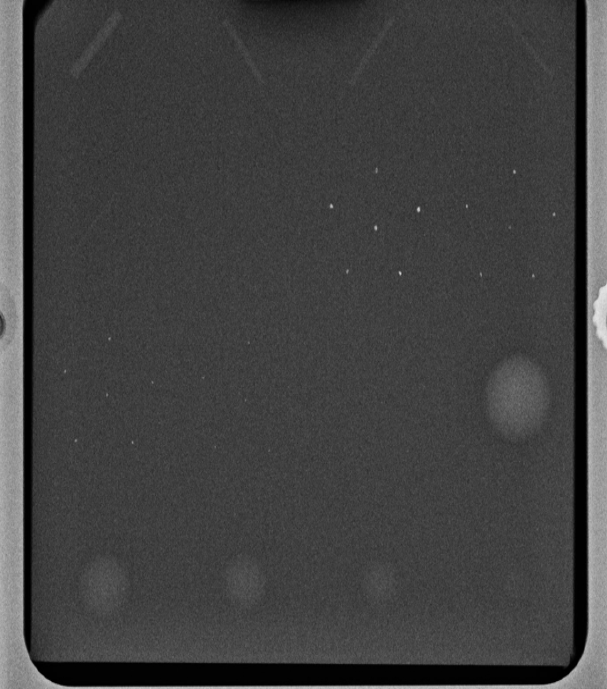
\includegraphics[width=0.5\linewidth]{images/AcrPhantom} 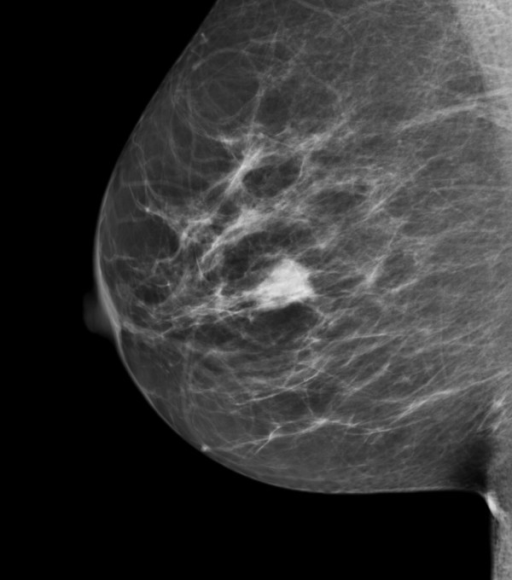
\includegraphics[width=0.5\linewidth]{images/Clinical} \caption{(A) Image of an ACR phantom, (B) Clinical image.}\label{fig:acrPhantomClinical}
\end{figure}

Fig. \ref{fig:acrPhantomClinical} (A -- B): (A) Image of an American College of Radiology mammography accreditation phantom. The phantom contains target objects consisting of six fibrils, five groups of microcalcifications, and five nodule-like objects. An image of the phantom is obtained daily, before the first patient is imaged, and is inspected by a technologist, who records the number of target objects of different types that are visible. On his 27" iMac monitor, the author sees four fibrils, three speck groups and four masses, which would be graded as a ``pass''. This is greatly simplified version of the test. The scoring accounts for irregular fibril or partially visible masses borders, etc., all of which is intended to get more objectivity out of the measurement. (B) A breast image showing an invasive cancer, located roughly in the middle of the image. Note the lack of similarity between the two images (A) and (B). The breast image is much more complex and there is more information, and therefore more to go wrong than with the phantom image. Moreover, there is variability between patients in contrast to the fixed image in (A). In the author's clinical experience, the phantom images interpreted visually are a poor predictor of clinical image quality.

One can perhaps appreciate the subjectivity of the measurement. Since the target locations are known, the technologist can claim to have detected it and the claim cannot be disproved; unless a claim is falsifiable, it is not science. While the QC team is trained to achieve repeatable measurements, the author has shown{[}30-34{]} that computer analysis of mammography phantom images (CAMPI) can achieve far greater precision and repeatability than human observer readings. Commercial software is currently available from various vendors that perform proprietary analysis of phantom images for various imaging systems (e.g., mammography machines, CT scanners, MRI scanners, ultrasound, etc.).

Fig. \ref{fig:acrPhantomClinical} (B) shows a mammogram with a mass-like cancer visible near it center. It is characterized by complex anatomical background, quite unlike the uniform background in the phantom image in Fig. \ref{fig:acrPhantomClinical} (A). In mammography 30\% of retrospectively visible lesions are missed at initial screening and radiologist variability can be as large as 40\% {[}35{]}. QC machine parameters (e.g., kVp, the kilovoltage accuracy) are usually measured to 1\% accuracy. It is ironic that the weak link, in the sense of greatest variability, is the radiologist but quality control and much effort is primarily focused on measuring/improving the physical parameters of the machine. This comment is meant to motivate clinical medical physicists, most of who are focused on QC, to become more aware about observer performance methods, where achieving better than 5\% accuracy is quite feasible{[}36{]}. The author believes there should be greater focus on improving radiologist performance, particularly those with marginal performance. Efforts in this direction, using ROC methods, are underway in the UK {[}37, 38{]} by Prof Alistair Gale and colleagues.

\hypertarget{image-quality-vs.-task-performance}{%
\section{Image quality vs.~task performance}\label{image-quality-vs.-task-performance}}

In this book, ``image quality'' is defined as the fidelity of the image with respect to some external gold standard of what the ideal image should look like, while ``task performance'' is how well a radiologist, using the image, accomplishes a given clinical task. For example, if one had an original Rembrandt and a copy, the image quality of the copy is perfect if even an expert appraiser cannot distinguish it from the original. The original painting is the ``gold standard''. If an expert can distinguish the copy from the original, its image quality is degraded. The amount of degradation is related to the ease with which the expert can detect the fraud.

A radiological image is the result of x-rays interactions within the patient and the image receptor. Here it is more difficult to define a gold standard. If it exists at all, the gold standard is expected to depend on what the image is being used for, i.e., the diagnostic task. An image suitable for soft-tissue disease diagnosis may not be suitable for diagnosis of bone disease. This is the reason why CT scanners have different soft-tissue and bone window/level settings. With clinical images, a frequently used approach is to have an expert rank-order the images, acquired via different methods, with respect to ``clinical appropriateness'' or ``clinical image quality''. The quotes are used to emphasize that these terms are hard to define objectively. In this approach, the gold standard is in the mind of the expert. Since experts have typically interpreted tens of thousands of images in the past, and have lived with the consequences of their decisions, there is considerable merit to using them to judge clinical image quality. However, experts do disagree and biases cannot be ruled out. This is especially true when a new imaging modality is introduced. The initial introduction of computed radiography (CR) was met with some resistance in the US among technologists, who had to learn a different way of obtaining the images that disrupted their workflow. There was also initial resistance from more experienced radiologists, who were uncomfortable with the appearance of the new images, i.e., their gold standard was biased in favor of the modality -- plain films -- that they were most familiar. The author is aware of at least one instance where CR had to be imposed by ``diktat'' from the Chairman of the department. Some of us are more comfortable reading printed material than viewing it on a computer screen, so this type of bias is understandable.

Another source of bias is patient variability, i.e., the gold standard depends on the patient. Some patients are easier to image than others are in the sense that their images are ``cleaner'', i.e., they depict anatomical structures that are known to be present more clearly. X-rays pass readily through a relatively slim patient (e.g., an athlete) and there are fewer scattered photons which degrade image quality{[}39, 40{]}, than when imaging a larger patient (e.g., an NFL linebacker). The image of the former will be clearer, the ribs, the heart shadow, the features of the lungs, etc., will be better visualized (i.e., closer to what is expected based on the anatomy) than the image of the linebacker. Similar differences exist in the ease of imaging women with dense breasts, containing a larger fraction of glandular tissue compared to women with fatty breasts. By imaging appropriately selected patients, one can exploit these facts to make one's favorite imaging system look better. {[}Prof.~Harold Kundel, one of the author's mentors, used to say: ``Tell me which modality you want to come out better and I will prepare a set of patient images to help you make your case''.{]}

\hypertarget{why-physical-measures-of-image-quality-are-not-enough}{%
\section{Why physical measures of image quality are not enough}\label{why-physical-measures-of-image-quality-are-not-enough}}

Both high spatial resolution and low noise are desirable characteristics. However, imaging systems do not come unambiguously separated as high spatial resolution and low noise vs.~low spatial resolution and high noise. There is generally an intrinsic imaging physics dictated tradeoff between spatial resolution and noise. Improving one makes the other worse. For example, if the digital image is smoothed with, for example, with a spatial filter, then noise will be smaller, because of the averaging of neighboring pixels, but the ability to resolve closely spaced structures will be compromised. Therefore, a more typical scenario is deciding whether the decreased noise justifies the accompanying loss of spatial resolution. Clearly the answer to this depends on the clinical task: if the task is detecting relatively large low contrast nodules, then some spatial smoothing may actually be beneficial, but if the task involves detecting small microcalcifications, often the precursors of cancer in the breast, then the smoothing will tend to reduce their visibility.

The problem with physical measures of image quality lies in relating them to clinical performance. Phantom images have little resemblance to clinical images, compare Fig. \ref{fig:acrPhantomClinical} (A) and (B). X-ray machines generally have automatic exposure control: the machines use a brief exposure to automatically sense the thickness of the patient from the detected x-rays. Based on this, the machine chooses the best combinations of technical factors (kVp and tube charge) and image processing. The machine has to be put in a special manual override mode to obtain reasonable images of phantoms, as otherwise the exposure control algorithm, which expects patient anatomy, is misled by the atypical nature of the ``patient'', compared to typical patient anatomy, into producing very poor phantom images. This type of problem makes it difficult to reproduce problems encountered using clinical images with phantom images. It has been the author's general experience that QC failures often lag clinical image quality reported problems: more often than not, clinical image quality problems are reported before QC measurements indicate a problem. This is not surprising since clinical images, e.g., Fig. \ref{fig:acrPhantomClinical} (B) are more complex and have more information{[}41{]}, both in the clinical and in the information theoretic sense{[}42{]}, than the much simpler phantom image shown in Fig. \ref{fig:acrPhantomClinical} (A), so there is more that can go wrong with clinical images than with phantom images. Manufacturers now design anthropomorphic phantoms whose images resemble human x-rays. Often these phantoms provide the option of inserting target objects at random locations; this is desired to get more objectivity out of the measurement. Now, if the technologist claims to have found the target, the indicated location can be used to determine if the target was truly detected.

To circumvent the possibility that changes in physical measurements on phantoms may not sensitively track changes in clinical image interpretations by radiologists, a measurement needs to include both the complexity of clinical images and radiologists as part of the measurement. Because of variability in both patient images and radiologist interpretations, such measurements are expected to be more complicated than QC measurements, so to be clear, the author is not advocating observer performance studies as part of QC. However, they could be built into a continuous quality improvement program, perhaps performed annually. Before giving an overview of the more complex methods, an alternative modeling driven approach, that is widely used, is described next.

\hypertarget{model-observers}{%
\section{Model observers}\label{model-observers}}

If one can adequately simulate (or model) the entire imaging process, then one can design mathematical measurements that can be used to decide if a new imaging system is an improvement over a conventional imaging system. Both new and conventional systems are modeled (i.e., reduced to formulae that can be evaluated). The field of model observers{[}43{]} is based on assuming this can be done. The FDA/CDRH has a research program called VICTRE: Virtual Imaging Clinical Trials for Regulatory Evaluation. Since everything is done on a computer, the method does not require time-consuming studies involving radiologists.

A simple example may elucidate the process (for more details one should consult the extensive literature on model observers). Suppose one simulates image noise by sampling a Gaussian random number generator and filling up the pixels in the image with the random samples. This simulates a non-diseased image. The number of such images could be quite large, e.g., 1000, limited only by one's patience. A second set of simulated diseased images is produced in which one samples a random number generator to create non-diseased images, as before, but this time one adds a small low-contrast but noiseless disk, possibly with Gaussian edges, to the center of each image. The procedure yields two sets of images, 1000 with noise only backgrounds and 1000 with different noise backgrounds and the superposed centered low contrast disk. One constructs a template whose shape is identical to that of the superposed disk (i.e., one does not simply measure peak contrast at the center of the lesion; rather the shape-dependent contrast of the disk is taken into account). One then calculates the cross-correlation of the template with each of the superposed disks{[}30, 44{]}. The cross correlation is the sum of the products of pixel values of corresponding pixels, one drawn from the template and the other drawn from the matching position on the disk image. {[}Details of this calculation are in Online Appendix 12.B of Chapter 12.{]} Because of random noise, the cross-correlations from different simulated diseased cases will not be identical, and one averages the 1000 values. Next one applies the template to the centers of the non-diseased images and computes the cross correlations as before. Because of the absence of the disk, the values will be smaller (assuming positive disk contrast). The difference between the average of the cross-correlations at disk locations and the average at disk-absent locations is the numerator of a signal to noise ratio (SNR) like quantity. The denominator is the standard deviation of the cross-correlations at disk-free locations. To be technical, the procedure yields the signal-to-noise-ratio (SNR) of the non-pre-whitening ideal observer{[}45{]}. It is an ideal mathematical ``observer'' in the sense that for white noise no human observer can surpass this level of performance{[}46, 47{]}.

Suppose the task is to evaluate two image-processing algorithms. One applies each algorithm to the 2000 images described above and measures SNR for each algorithm. The one yielding the higher SNR, after accounting for variability in the measurements, is the superior algorithm.

Gaussian noise images are not particularly ``clinical'' in appearance. If one filters the noise appropriately, one can produce simulated images that are similar to non-diseased backgrounds observed in mammography{[}48-50{]}. Other techniques exist for simulating statistically characterized lumpy backgrounds that are a closer approximation to some medical images{[}51{]}.

Having outlined one of the alternatives, one is ready for the methods that form the subject matter of this book.

\hypertarget{measuring-observer-performance-four-paradigms}{%
\section{Measuring observer performance: four paradigms}\label{measuring-observer-performance-four-paradigms}}

Observer performance measurements come in different ``flavors'', types or paradigms. In the current context, a paradigm is an agreed-upon method for collecting the data. A given paradigm can lend itself to different analyses. In historical order the paradigms are: (1) the receiver operating characteristic (ROC) paradigm {[}1, 2, 7, 52, 53{]}; (2) the free-response ROC (FROC) paradigm {[}54, 55{]}; (3) the location ROC (LROC) paradigm {[}56, 57{]} and (4) the region of interest (ROI) paradigm {[}58{]}. Each paradigm assumes that the truth is known independently of the modalities to be compared. This implies that one cannot use diagnoses from one of the modalities to define truth -- if one did, the measurement would be biased in favor of the modality used to define truth. It is also assumed that the true disease status of the image is known to the researcher but the radiologist is ``blinded'' to this information.

In the ROC paradigm the observer renders a single decision per image. The decision could be communicated using a binary scale (ex. 0 or 1) or declared by use of the terms ``negative'' or ``positive,'' abbreviations of ``negative for disease'' (the radiologist believes the patient is non-diseased) and ``positive for disease'' (the radiologist believes the patient is diseased), respectively. Alternatively, the radiologist could give an ordered numeric label, termed a rating, to each case where the rating is a number with the property that higher values correspond to greater radiologist's confidence in presence of disease. A suitable ratings scale could be the consecutive integers 1 through 6, where ``1'' is ``definitely non-diseased'' and ``6'' is ``definitely diseased''.

If data is acquired on a binary scale, then the performance of the radiologist can be plotted as a single operating point on an ROC plot. The x-axis of the plot is false positive fraction (FPF), i.e., the fraction of non-diseased cases incorrectly diagnosed as diseased. The y-axis of the plot is true positive fraction (TPF), i.e., the fraction of diseased cases correctly diagnosed as diseased. Models have been developed to fit binary or multiple rating datasets. These models predict continuous curves, or operating characteristics, along which an operating point can move by varying the radiologist's reading style. The reading style is related to the following concept: based on the evidence in the image, how predisposed is a radiologist to declaring a case as diseased. A ``lenient'', ``lax'' or ``liberal'' reporting style radiologist is very predisposed even with scant evidence. A ``strict'' or ``conservative'' reporting style radiologist requires more evidence before declaring a patient as diseased. This brief introduction to the ROC was given to explain the term ``operating characteristic'' in ROC. The topic is addressed in more detail in Chapter 02.

In the FROC paradigm the observer marks and rates all regions in the image that are sufficiently suspicious for disease. A mark is the location of the suspicious region and the rating is an ordered label, characterizing the degree of suspicion attached to the suspicious region. In the LROC paradigm the observer gives an overall ROC-type rating to the image, and indicates the location of the most suspicious region in the image. In the ROI paradigm the researcher divides each image into a number of adjacent non-overlapping regions of interest (ROIs) that cover the clinical area of interest. The radiologist's task is to evaluate each ROI for presence of disease and give an ROC-type rating to it.

\hypertarget{basic-approach-to-the-analysis}{%
\subsection{Basic approach to the analysis}\label{basic-approach-to-the-analysis}}

The basic approach is to obtain data, according to one of the above paradigms, from a group of radiologists interpreting a common set of images in one or more modalities. The way the data is collected, and the structure of the data, depends on the selected paradigm. The next step is to adopt an objective measure of performance, termed a figure or merit (FOM) and a procedure for estimating it for each modality-reader combination. Assuming two modalities, e.g., a new modality and the conventional one, one averages FOM over all readers within each modality. If the difference between the two averages (new modality minus the conventional one) is positive, that is an indication of improvement. Next comes the statistical part: is the difference large enough so as to be unlikely to be due to chance. This part of the analysis, termed significance testing, yields a probability, or p-value, that the observed difference or larger could result from chance even though the modalities have identical performances. If the p-value is very small, that it is taken as evidence that the modalities are not identical in performance, and if the difference is in the right direction, the new modality is judged better.

\hypertarget{historical-notes}{%
\subsection{Historical notes}\label{historical-notes}}

The term ``receiver operating characteristic'' (ROC) traces its roots to the early 1940s. The ``receiver'' in ROC literally denoted a pulsed radar receiver that detects radio waves bounced off objects in the sky, the obvious military application being to detect enemy aircraft. Sometimes the reflections were strong compared to receiver electronic noise and other sources of noise and the operator could confidently declare that the reflection indicated the presence of aircraft and the operator was correct. This combination of events was termed a true positive (TP). At other times the aircraft was present but due to electronic noise and reflections off clouds, the operator was not confident enough to declare ``aircraft present'' and this combination of events was termed a false negative (FN). Two other types of decisions can be discerned when there was no aircraft in the field of view: (1) the operator mistook reflections from clouds or perhaps a flock of large birds and declared ``aircraft present'', termed a false positive (FP). (2) The operator did not declare ``aircraft present'' because the reflected image was clear of noise or false reflections and the operator felt confident in a negative decision, termed a true negative (TN). Obviously, it was desirable to maximize correct decisions (TPs and TNs) while minimizing incorrect decisions (FNs and FPs). Scientists working on this problem analyzed it as a generic signal detection problem, where the signal was the aircraft reflection and the noise was everything else. A large field called signal detection theory (SDT) emerged{[}59{]}. However, even at this early stage, it must have been apparent to the researchers that the problem was incomplete in a key respect: when the operator detects a suspicious signal, there is a location (specifically an azimuth and altitude associated with it. The operator could be correct in stating ``aircraft present'' but direct the interceptors to the wrong location. Additionally, there could be multiple enemy aircraft present, but the operator is only allowed the ``aircraft present'' and ``aircraft absent'' responses, which fail to allow for multiplicity of suspected aircraft locations. This aspect was not recognized, to the best of the author's knowledge, until Egan coined the term ``free-response'' in the auditory detection context{[}54{]}.

Having briefly introduced the different paradigms, two of which, namely the ROC and the FROC, will be the focus of this book, it is appropriate to see how these measurements fit in with the different types of measurements possible in assessing imaging systems.

\hypertarget{hierarchy-of-assessment-methods}{%
\section{Hierarchy of assessment methods}\label{hierarchy-of-assessment-methods}}

The methods described in this book need to be placed in context of a six-level hierarchy of assessment methods{[}7, 60{]}. The cited paper by Fryback and Thornbury on ``The Efficacy of Diagnostic Imaging'' is a highly readable account, which also gives a more complete overview of this field, including key contributions by Yerushalmy{[}61{]} and Lusted{[}62{]}. The term efficacy is defined generically as ``the probability of benefit to individuals in a defined population from a medical technology applied for a given medical problem under ideal conditions of use''. Demonstration of efficacy at each lower level is a necessary but not sufficient condition to assure efficacy at higher level. The different assessment methods are, in increasing order of efficacy : technical, diagnostic accuracy, diagnostic thinking, therapeutic, patient outcome and societal, Table \ref{tab:FrybackThornbury}.

Table \ref{tab:FrybackThornbury}: Fryback and Thornbury proposed hierarchy of assessment methods. Demonstration of efficacy at each lower level is a necessary but not sufficient condition to assure efficacy at higher level. {[}MTF = modulation transfer function; NPS(f) = noise power spectra as a function of spatial frequency f; DQE(f) = detective quantum efficiency{]}

\begin{table}

\caption{\label{tab:FrybackThornbury}FrybackThornbury hierarchy of efficacies.}
\centering
\begin{tabular}[t]{l|l}
\hline
Level Designation & Essential Characteristic\\
\hline
1. Technical efficacy & Engineering measures: MTF, NPS, DQE\\
\hline
2. Diagnostic accuracy efficacy & Sensitivity, specificity, ROC or FROC area\\
\hline
3. Diagnostic thinking efficacy & Positive and negative predictive values\\
\hline
4. Therapeutic efficacy & Treatment benefits from imaging test?\\
\hline
5. Patient outcome efficacy & Patients benefit from imaging test?\\
\hline
6. Societal efficacy & Society benefits from imaging test?\\
\hline
\end{tabular}
\end{table}

The term ``clinical relevance'' is used rather loosely in the literature. The author is not aware of an accepted definition of ``clinical relevance'' apart from its obvious English language meaning. As a working definition the author has proposed {[}63{]} that the clinical relevance of a measurement be defined as its hierarchy-level. A level-5 patient outcome measurement (do patients, on the average, benefit from the imaging study) is clinically more relevant than a technical measurement like noise on a uniform background phantom or an ROC study. This is because it relates directly to the benefit, or lack thereof, to a group of patients (it is impossible to define outcome efficacy at the individual patient level -- at the patient level outcome is a binary random variable, e.g., 1 if the outcome was good or 0 if the outcome was bad).

One could make physical measurements ad-infinitum, but one cannot (yet) predict the average benefit to patients. Successful virtual clinical trials would prove the author wrong. ROC studies are more clinically relevant than physical measurements, and it is more likely that a modality with higher performance will yield better outcomes, but it is not a foregone conclusion. Therefore, higher-level measurements are needed.

However, the time and cost of the measurement increases rapidly with the hierarchy level. Technical efficacy, although requiring sophistical mathematical methods, take relatively little time. ROC and FROC, both of which are level-2 diagnostic accuracy measurements, take more time, often a few months to complete. However, since ROC measurements include the entire imaging chain and the radiologist, they are more clinically relevant than technical measurements, but they do not tell us the effect on diagnostic thinking. After the results of ``live'' interpretations are available, e.g., patients are diagnosed as diseased or non-diseased, what does the physician do with the information. Does the physician recommend further tests or recommends immediate treatment. This is where the level-3 measurements come in, which measure the effect on diagnostic thinking. Typical level-3 measurements are positive predictive value (PPV) and negative predictive value (NPV). PPV is the probability that the patient is actually diseased when the diagnosis is diseased and NPV is the probability that the patient is actually non-diseased when the diagnosis is non-diseased. These are discussed in more detail in Chapter 02.

Unlike level-2 measurements, PPV and NPV depend on disease prevalence. As an example consider breast cancer which (fortunately) has low prevalence, about 0.005. Before the image is interpreted and lacking any other history, the mammographer knows only there is a five in 1000 chance that the woman has breast cancer. After the image is interpreted, the mammographer has more information. If the image was interpreted as diseased, the confidence in presence of cancer increases. For an expert mammographer typical values of sensitivity and specificity are 80\% and 90\%, respectively (these terms will be explained in the next chapter; sensitivity is identical to true positive fraction and specificity is 1-false positive fraction). It will be shown (in Chapter 02, §2.9.2) that for this example PPV is only 0.04. In other words, even though an expert interpreted the screening mammogram as diseased, the chance that the patient actually has cancer is only 4\%. Obviously more tests are needed before one knows for sure if the patient has cancer -- this is the reason for the recall and the subsequent diagnostic workup referred to in §1.2.2. The corresponding NPV is 0.999. Negative interpretations by experts are definitely good news for the affected patients and these did not come directly from an ROC study, or physical measurements, rather they came from actual ``live'' clinical interpretations. Again, NPV and PPV are defined as averages over a group of patients. For example, the 4\% chance of cancer following a positive diagnosis is good news, on the average. An unlucky patient could be one of the four-in-100-patients that has cancer following a positive screening diagnosis.

While more relevant than ROC, level-3 measurements like PPV and NPV are more difficult to conduct than ROC studies {[}18{]} -- they involve following, in real time, a large cohort of patients with images interpreted under actual clinical conditions. Level 4 and higher measurements, namely therapeutic, patient outcome and societal, are even more difficult and are sometimes politically charged, as they involve cost benefit considerations.

\hypertarget{overview-of-the-book-and-how-to-use-it}{%
\section{Overview of the book and how to use it}\label{overview-of-the-book-and-how-to-use-it}}

For the most part the book follows the historical development, i.e., it starts with chapters on ROC methodology, chapters on significance testing, chapters on FROC methodology, chapters on advanced topics and appendices. Not counting Chapter 01, the current chapter, the book is organized five Parts (A - E).

\hypertarget{overview-of-the-book}{%
\subsection{Overview of the book}\label{overview-of-the-book}}

\hypertarget{part-a-the-roc-paradigm}{%
\subsubsection{Part A: The ROC paradigm}\label{part-a-the-roc-paradigm}}

Part A describes the ROC (receiver operating characteristic) paradigm. Chapter 02 describes the binary decision task. Terminology that is important to master, such as accuracy, sensitivity, specificity, disease prevalence, positive and negative predictive values is introduced. Chapter 03 introduces the important concepts of decision variable, the reporting threshold, and how the latter may be manipulated by the researcher and it introduces the ROC curve. Chapter 04 reviews the widely used ratings method for acquiring ROC data. Chapter 06 introduces the widely used binormal model for fitting ratings data. The chapter is heavy on mathematical and computational aspects, as it is intended to take the mystery out of these techniques, which are used in subsequent chapters. The data fitting method, pioneered by Dorfman and Alf in 1969, is probably one of the most used algorithms in ROC analysis. Chapter 07 describes sources of variability affecting any performance measure, and how they can be estimated.

\hypertarget{part-b-the-statistics-of-roc-analysis}{%
\subsubsection{Part B: The statistics of ROC analysis}\label{part-b-the-statistics-of-roc-analysis}}

Part B describes the specialized statistical methods needed to analyze ROC data, in particular how to analyze data originating from multiple readers interpreting the same cases in multiple modalities. Chapter 08 introduces hypothesis-testing methodology, familiar to statisticians, and the two types of errors that the researcher wishes to control, the meaning of the ubiquitous p-value and statistical power. Chapter 09 focuses on the Dorfman-Berbaum-Metz method, with improvements by Hillis. Relevant formulae, mostly from publications by Prof.~Steven Hillis, are reproduced without proofs (it is the author's understanding that Dr.~Hillis is working on a book on his specialty, which should nicely complement the minimalistic-statistical description approach adopted in this book). Chapter 10 describes the Obuchowski-Rockette method of analyzing MRMC ROC data, with Hillis' improvements. Chapter 11 describes sample size estimation in an ROC study.

\hypertarget{part-c-the-froc-paradigm}{%
\subsubsection{Part C: The FROC paradigm}\label{part-c-the-froc-paradigm}}

Part C is unique to this book. Anyone truly wishing to understand human observer visual search performance needs to master it. The payoff is that the concepts, models and methods described here apply to almost all clinical tasks. Chapter 17 and Chapter 18 are particularly important. These were difficult chapters to write and they will take extra effort to comprehend. However, the key findings presented in these chapters and their implications should strongly influence future observer performance research. If the potential of the findings is recognized and used to benefit patients, by even one reader, the author will consider this book a success. Chapter 19 describes how to analyze FROC data and report the results.

\hypertarget{part-d-advanced-topics}{%
\subsubsection{Part D: Advanced topics}\label{part-d-advanced-topics}}

Some of the chapters in Part D are also unique to this book. Chapter 20 discusses proper ROC curve fitting and software. The widely used bivariate binormal model, developed around 1980, but never properly documented, is explained in depth, and a recent extension of it that works with any dataset is described in Chapter 21. Also described is a method for comparing (standalone) CAD to radiologists, Chapter 22. Standalone CAD performance is rarely measured, which is a serious mistake, for which we are all currently paying the price. It does not work for masses in mammography{[}64-66{]}. In the UK CAD is not used, instead they rely on double readings by experts, which is actually the superior approach, given the current low bar used in the US for CAD to be considered a success. Chapter 23, co-authored by Mr.~Xuetong Zhai, a graduate student, describes validation of the CAD analysis method described in Chapter 22. It describes constructing a single-modality multiple-reader ratings data simulator. The method is extendible to multiple-modality multiple-reader datasets.

\hypertarget{part-e-appendices-tba}{%
\subsubsection{Part E: Appendices (TBA)}\label{part-e-appendices-tba}}

Part E contains two online chapters. Online Chapter 24 is a description of 14 datasets, all but 2 of them collected by the author over years of collaborations with researchers who conducted the studies and on which the author helped with analysis and sometimes with manuscript preparation. The datasets provide a means to demonstrate analysis techniques and to validate fitting methods. Finally, Online Chapter 25, co-authored by Mr.~Xuetong Zhai, is a user-manual for the RJafroc package. Since RJafroc is used extensively in the book, this is expected to be a useful ``go-to'' chapter for the reader. The choice to put these chapters online is to allow the author to update the datasets with new files as they become available and to update the documentation of RJafroc as new features are added.

\hypertarget{how-to-use-the-book}{%
\subsection{How to use the book}\label{how-to-use-the-book}}

Each chapter consists of the physical book chapter that one is reading. Additionally, there are good chances that the online directory corresponding to this book will contain two directories, one called software and the other called Supplementary Material. The software directory contains ``ready to run'' code that is referenced in the book chapter text. When one sees such a reference in a chapter, the reader should open the relevant file and run it. Detailed directions are provided in the Online Appendix corresponding to each chapter.

Those new to the field should read the chapters in sequence. It is particularly important to master Part A. Part B presents the statistical analysis at a level accessible to the expected readers of this book, namely the user community. The only way to really understand this part is to apply the described methods and codes to the online datasets. Understanding the formulae in this part, especially those relating to statistical hypothesis testing, requires statistical expertise, which could lead the average reader in unproductive directions. It is best to accept the statisticians' formulae and confirm that they work. How to determine if a method ``works'' will be described. Readers with prior experience in the field may wish to ``skim'' chapters. If they do, it is strongly recommended that they at least run and understand the software examples. This will prepare them for the more complex code in later chapters.

This concludes the introduction of the book.

\hypertarget{preliminaries-Summary}{%
\section{Summary}\label{preliminaries-Summary}}

\hypertarget{preliminaries-Discussion}{%
\section{Discussion}\label{preliminaries-Discussion}}

\hypertarget{preliminaries-references}{%
\section{References}\label{preliminaries-references}}

\hypertarget{binaryTask0}{%
\chapter{The Binary Task}\label{binaryTask0}}

\hypertarget{binaryTask0Intro}{%
\section{Introduction}\label{binaryTask0Intro}}

In the previous chapter four observer performance paradigms were introduced: the receiver operating characteristic (ROC), the free-response ROC (FROC), the location ROC (LROC) and the region of interest (ROI). The next few chapters focus on the ROC paradigm, where each case is rated for confidence in presence of disease. While a multiple point rating scale is generally used, in this chapter it is assumed that the ratings are binary, and the allowed values are ``1'' vs.~``2''. Equivalently, the ratings could be ``non-diseased'' vs.~``diseased'', ``negative'' vs.~``positive'', etc. In the literature this method of data acquisition is also termed the ``yes/no'' procedure \citep{RN298, RN346}. The reason for restricting, for now, to the binary task is that the multiple rating task can be shown to be equivalent to a number of simultaneously conducted binary tasks. Therefore, understanding the simpler method is a good starting point.

Since the truth is also binary, this chapter could be named the binary-truth binary-decision task. The starting point is a 2 x 2 table summarizing the outcomes in such studies and useful fractions that can be defined from the counts in this table, the most important ones being true positive fraction (TPF) and false positive fraction (FPF). These are used to construct measures of performance, some of which are desirable from the researcher's point of view, but others are more relevant to radiologists. The concept of disease prevalence is introduced and used to formulate relations between the different types of measures. An R example of calculation of these quantities is given that is only slightly more complicated than the demonstration in the prior chapter.

\hypertarget{binaryTask0Truth}{%
\section{The fundamental 2x2 table}\label{binaryTask0Truth}}

In this book, the term case is used for images obtained for diagnostic purposes, of a patient; often multiple images of a patient, sometimes from different modalities, are involved in an interpretation; all images of a single patient, that are used in the interpretation, are collectively referred to as a case. A familiar example is the 4-view presentation used in screening mammography, where two views of each breast are available for viewing.

Let \(D\) represent the radiologist's decision, with \(D=1\) representing the decision ``case is non-diseased'' and \(D=2\) representing the decision ``case is diseased''. Let \(T\) denote the truth with \(T=1\) representing ``case is actually non-diseased'' and \(T=2\) representing ``case is actually diseased''. Each decision, one of two values, will be associated with one of two truth states, resulting in an entry in one of 4 cells arranged in a 2 x 2 layout, termed the decision vs.~truth table, Table \ref{tab:binaryTask0truthTable}, which is of fundamental importance in observer performance. The cells are labeled as follows. The abbreviation \(TN\), for true negative, represents a \(D=1\) decision on a \(T=1\) case. \(FN\), for false negative, represents a \(D=1\) decision on a \(T=2\) case (also termed a ``miss''). \(FP\), for false positive, represents a \(D=2\) decision on a \(T=1\) case (a ``false-alarm'') and \(TP\), for true positive, represents a \(D=2\) decision on a \(T=2\) case (a ``hit'').

\begin{table}

\caption{\label{tab:binaryTask0truthTable}Truth Table.}
\centering
\begin{tabular}[t]{l|l|l}
\hline
  & T=1 & T=2\\
\hline
D=1 & TN & FN\\
\hline
D=2 & FP & TP\\
\hline
\end{tabular}
\end{table}

Table \ref{tab:binaryTask0truthTable2} shows the numbers of decisions in each of the four categories defined in Table \ref{tab:binaryTask0truthTable}. Specifically, \(n(TN)\) is the number of true negative decisions, \(n(FN)\) is the number of false negative decisions, etc. The last row is the sum of the corresponding columns. The sum of the number of true negative decisions \(n(TN)\) and the number of false positive decisions \(n(FP)\) must equal the total number of non-diseased cases, denoted \(K_1\). Likewise, the sum of the number of false negative decisions \(n(FN)\) and the number of true positive decisions \(n(TP)\) must equal the total number of diseased cases, denoted \(K_2\). The last column is the sum of the corresponding rows. The sum of the number of true negative \(n(TN)\) and false negative \(n(FN)\) decisions is the total number of negative decisions, denoted \(n(N)\). Likewise, the sum of the number of false positive \(n(FP)\) and true positive \(n(TP)\) decisions is the total number of positive decisions, denoted \(n(P)\). Since each case yields a decision, the bottom-right corner cell is \(n(N) + n(P)\), which must also equal \(K_1+K_2\), the total number of cases \(K\). These statements are summarized in Eqn. \eqref{eq:binaryTask0TruthTableEqns}.

\begin{equation} 
\left.\begin{aligned}
K_1&=n(TN)+n(FP)\\ 
K_2&=n(FN)+n(TN)\\ 
n(N)&=n(TN)+n(FN)\\ 
n(P)&=n(TP)+n(FP)\\
K=K_1+K_2&=n(N)+n(P)
\end{aligned}\right\}
\label{eq:binaryTask0TruthTableEqns}
\end{equation}

\begin{table}

\caption{\label{tab:binaryTask0truthTable2}Cell counts.}
\centering
\begin{tabular}[t]{l|l|l|l}
\hline
  & T=1 & T=2 & RowSums\\
\hline
D=1 & n(TN) & n(FN) & n(N)=n(TN)+n(FN)\\
\hline
D=2 & n(FP) & n(TP) & n(P)=n(FP)+n(TP)\\
\hline
ColSums & $K_1$=n(TN)+n(FP) & $K_2$=n(FN)+n(TP) & $K=K_1+K_2$=n(N)+n(P)\\
\hline
\end{tabular}
\end{table}

\hypertarget{sensitivity-and-specificity}{%
\section{Sensitivity and specificity}\label{sensitivity-and-specificity}}

The notation \(P(D|T)\) indicates the probability of diagnosis D given truth state T (the vertical bar symbol is used to denote a conditional probability, i.e., what is to the left of the vertical bar depends on the condition appearing to the right of the vertical bar being true).

\begin{equation} 
P(D|T) = P(\text{diagnosis is D} | \text{truth is T})
\label{eq:binaryTask0PDGivenT}
\end{equation}

Therefore the probability that the radiologist will diagnose ``case is diseased'' when the case is actually diseased is \(P(D=2|T=2)\), which is the probability of a true positive \(P(TP)\).

\begin{equation} 
P(TP) = P(\text{D = 2} | \text{T = 2})
\label{eq:binaryTask0PTP}
\end{equation}

Likewise, the probability that the radiologist will diagnose ``case is non-diseased'' when the case is actually diseased is \(P(D=1|T=2)\), which is the probability of a false negative \(P(FN)\).

\begin{equation} 
P(FN) = P(\text{D = 1} | \text{T = 2})
\label{eq:binaryTask0PFN}
\end{equation}

The corresponding probabilities for non-diseased cases, \(P(TN)\) and \(P(FP)\), are defined by:

\begin{equation} 
\left.\begin{aligned}
P(TN)&=P(D=1|T=1)\\ 
\\
P(FP)&=P(D=2|T=1)
\end{aligned}\right\}
\label{eq:binaryTask0PTNFP}
\end{equation}

Since the diagnosis must be either \(D=1\) or \(D=2\), for each truth state the probabilities on non-diseased and diseased cases must sum to unity:

\begin{equation} 
\left.\begin{matrix}
P(D=1|T=1)+P(D=2|T=1)=1\\ 
\\  
P(D=1|T=2)+P(D=2|T=2)=1
\end{matrix}\right\}
\label{eq:binaryTask0PSumsToUnity}
\end{equation}

Equivalently, these equations can be written:

\begin{equation} 
\left.\begin{matrix}
P(TN)+P(FP)=1\\ 
\\
P(FN)+P(TP)=1
\end{matrix}\right\}
\label{eq:binaryTask0PSumsToUnity2}
\end{equation}

Comments:

\begin{itemize}
\tightlist
\item
  An easy way to remember Eqn. \eqref{eq:binaryTask0PSumsToUnity2} is to start by writing down the probability of one of the four probabilities, e.g., \(P(TN)\), and ``reversing'' both terms inside the parentheses, i.e., \(T \Rightarrow F\), and \(N \Rightarrow P\). This yields the term \(P(FP)\) which when added to the previous probability, \(P(TN)\), yields unity, i.e., the 1st equation in Eqn. \eqref{eq:binaryTask0PSumsToUnity2}.
\item
  Because there are two equations in four unknowns, only two of the four probabilities, one per equation, are independent. By tradition these are chosen to be \(P(D=1|T=1)\) and \(P(D=2|T=2)\), i.e., \(P(TN)\) and \(P(TP)\), which happen to be the probabilities of correct decisions on non-diseased and diseased cases, respectively. The two basic probabilities are so important that they have names: \(P(D=2|T=2)=P(TP)\) is termed sensitivity (Se) and \(P(D=1|T=1)=P(TN)\) is termed specificity (Sp):
\end{itemize}

\begin{equation} 
\left.\begin{matrix}
\text{Se}=P(TP)=P(D=2|T=2)\\ 
\\
\text{Sp}=P(TN)=P(D=1|T=1)
\end{matrix}\right\}
\label{eq:binaryTask0SeSp}
\end{equation}

The radiologist can be regarded as a diagnostic ``test'' yielding a binary decision under the binary truth condition. More generally, any test (e.g., a blood test for HIV) yielding a binary result (positive or negative) under a binary truth condition is said to be sensitive if it correctly detects the diseased condition most of the time. The test is said to be specific if it correctly detects the non-diseased condition most of the time. Sensitivity is how correct the test is at detecting a diseased condition, and specificity is how correct the test is at detecting a non-diseased condition.

\hypertarget{reasons-for-the-names-sensitivity-and-specificity}{%
\subsection{Reasons for the names sensitivity and specificity}\label{reasons-for-the-names-sensitivity-and-specificity}}

It is important to understand the reason for these names and an analogy may be helpful. Most of us are sensitive to temperature, especially if the choice is between ice-cold vs.~steaming hot. The sense of touch is said to be sensitive to temperature. One can imagine some neurological condition rendering a person hypersensitive to temperature, such that the person responds ``hot'' no matter what is being touched. For such a person the sense of touch is not very specific, as it is unable to distinguish between the two temperatures. This person would be characterized by unit sensitivity (since the response is ``hot'' to all steaming hot objects) and zero specificity (since the response is never ``cold'' to ice-cold objects). Likewise, a different neurological condition could render a person hypersensitive to cold, and the response is ``cold'' no matter what is being touched. Such a person would have zero sensitivity (since the response is never ``hot'' when touching steaming hot) and unit specificity (since the response is ``cold'' when touching ice-cold). Already one suspects that there is an inverse relation between sensitivity and specificity.

\hypertarget{estimating-sensitivity-and-specificity}{%
\subsection{Estimating sensitivity and specificity}\label{estimating-sensitivity-and-specificity}}

Sensitivity and specificity are the probabilities of correct decisions, over diseased and non-diseased cases, respectively. The true values of these probabilities would require interpreting all diseased and non-diseased cases in the entire population of cases. In reality, one has a finite sample of cases and the corresponding quantities, calculated from this finite sample, are termed estimates. Population values are fixed, and in general unknown, while estimates are random variables. Intuitively, an estimate calculated over a larger number of cases is expected to be closer to the true or population value than an estimate calculated over a smaller number of cases.

Estimates of sensitivity and specificity follow from counting the numbers of TP and TN decisions in Table 2.2 and dividing by the appropriate denominators. For sensitivity, the appropriate denominator is the number of actually diseased cases, namely , and for specificity, the appropriate denominator is the number of actually non-diseased cases, namely . The estimation equations for sensitivity specificity are (estimates are denoted by the ``hat'' or circumflex symbol \^{}):

\begin{equation} 
\left.\begin{matrix}
\widehat{\text{Se}}=\widehat{P(TP)}=\frac{n(TP)}{K_2}\\
\\ 
\widehat{\text{Sp}}=\widehat{P(TN)}=\frac{n(TN)}{K_1}
\end{matrix}\right\}
\label{eq:binaryTask0SeSpEstimates}
\end{equation}

The ratio of the number of TP decisions to the number of actually diseased cases is termed true positive fraction \(\widehat{TPF}\), which is an estimate of sensitivity, or equivalently, an estimate of \(\widehat{P(TP)}\). Likewise, the ratio of the number of TN decisions to the number of actually non-diseased cases is termed true negative fraction \(\widehat{TNF}\), which is an estimate of specificity, or equivalently, an estimate of \(\widehat{P(TN)}\). The complements of \(\widehat{TPF}\) and \(\widehat{TNF}\) are termed false negative fraction \(\widehat{FNF}\) and false positive fraction \(\widehat{FPF}\), respectively.

\hypertarget{disease-prevalence}{%
\section{Disease prevalence}\label{disease-prevalence}}

Disease prevalence, often abbreviated to prevalence, is defined as the actual or true probability that a randomly sampled case is of a diseased patient, i.e., the fraction of the entire population that is diseased. It is denoted \(P(D|pop)\) when patients are randomly sampled from the population (``pop'') and otherwise it is denoted \(P(D|lab)\), where the condition ``lab'' stands for a laboratory study, where cases may be artificially enriched, and thus not representative of the population value:

\begin{equation} 
\left.\begin{matrix}
P(D|\text{pop})=P(T=2|\text{pop})\\
\\ 
P(D|\text{lab})=P(T=2|\text{lab})
\end{matrix}\right\}
\label{eq:binaryTask0DisPrev}
\end{equation}

Since the patients must be either diseased on non-diseased, it follows with either sampling method, that:

\begin{equation} 
\left.\begin{aligned}
P(T=1|\text{pop})+P(T=2|\text{pop})&=1\\
\\
P(T=1|\text{lab})+P(T=2|\text{lab})&=1
\end{aligned}\right\}
\end{equation}

If a finite number of patients are sampled randomly from the population the fraction of diseased patients in the sample is an estimate of true disease prevalence.

\begin{equation} 
\left.\begin{matrix}
\widehat{P(D|\text{pop})}=
\frac{K_2}{K_1+K_2}
\end{matrix}\right|_{pop}
\label{eq:binaryTask0DisPrevEst}
\end{equation}

It is important to appreciate the distinction between true (population) prevalence and laboratory prevalence. As an example, true disease prevalence for breast cancer is about five per 1000 patients in the US, but most mammography studies are conducted with comparable numbers of non-diseased and diseased cases:

\begin{equation} 
\left.\begin{aligned}
\widehat{P(D|\text{pop})}&\sim 0.005\\
\\
\widehat{P(D|\text{lab})}&\sim 0.5\gg \widehat{P(D|\text{pop})}
\end{aligned}\right\}
\label{eq:binaryTask0DisPrevLabVsPop}
\end{equation}

\hypertarget{accuracy}{%
\section{Accuracy}\label{accuracy}}

Accuracy is defined as the fraction of all decisions that are in fact correct. Denoting it by \(Ac\) one has for the corresponding estimate:

\begin{equation} 
\widehat{Ac}=\frac{n(TN)+n(TP)}{n(TN)+n(TP)+n(FP)+n(FN)}
\label{eq:binaryTask0AccuracyEst}
\end{equation}

The numerator is the total number of correct decisions and the denominator is the total number of decisions. An equivalent expression is:

\begin{equation} 
\widehat{Ac}=\widehat{Sp}\widehat{P(!D)}+\widehat{Se}\widehat{P(D)}
\label{eq:binaryTask0AccuracyEst2}
\end{equation}

The exclamation mark symbol is used to denote the ``not'' or negation operator. For example, \(P(!D)\) means the probability that the patient is not diseased. Eqn. \eqref{eq:binaryTask0AccuracyEst2} applies equally to laboratory or population studies, \emph{provided sensitivity and specificity are estimated consistently}. One cannot combine a population estimate of prevalence with a laboratory measurement of sensitivity and / or specificity.

Eqn. \eqref{eq:binaryTask0AccuracyEst2} can be understood from the following argument. \(\widehat{Sp}\) is the fraction of correct (i.e., negative) decisions on non-diseased cases. Multiplying this by \(\widehat{P(!D)}\) yields \(\widehat{Sp} \widehat{P(!D)}\), the fraction of correct negative decisions on all cases. Similarly, \(\widehat{Sp}\) is the fraction of correct positive decisions on all cases. Therefore, their sum is the fraction of (all, i.e., negative and positive) correct decisions on all cases. A formal mathematical derivation follows. The terms on the right hand side of Eqn. \eqref{eq:binaryTask0SeSpEstimates} can be ``turned around'' yielding:

\begin{equation} 
\left.\begin{matrix}
n(TP)=K_2 \widehat{Se}\\ 
\\
n(TN)=K_1 \widehat{Sp}
\end{matrix}\right\}
\label{eq:binaryTask0nTpnTN}
\end{equation}

Therefore,

\begin{equation} 
\begin{aligned}
\widehat{Ac}&=\frac{n(TN)+n(TP)}{K}\\
\\
&=\frac{K_1 \widehat{Sp}+K_2 \widehat{Se}}{K}\\
\\
&=\widehat{Sp} \widehat{P(!D)}+\widehat{Se}\widehat{P(D)}
\end{aligned}
\label{eq:binaryTask0AccuracyDeriv}
\end{equation}

\hypertarget{negative-and-positive-predictive-values}{%
\section{Negative and positive predictive values}\label{negative-and-positive-predictive-values}}

Sensitivity and specificity have desirable characteristics insofar as they reward the observer for correct decisions on actually diseased and actually non-diseased cases, respectively, so these quantities are expected to be independent of disease prevalence; one is dividing by the relevant denominator, so increased numbers of non-diseased cases are balanced by a corresponding increased number of correct decisions on non-diseased cases, and likewise for diseased cases. However, radiologists interpret cases in a ``mixed'' situation where cases could be positive or negative for disease and disease prevalence plays a crucial role in their decision-making -- this point will be clarified shortly. Therefore, a measure of performance that is desirable from the researcher's point of view is not necessarily desirable from the radiologist's point of view. It should be obvious that if most cases are non-diseased, i.e., disease prevalence is close to zero, specificity, being correct on non-diseased cases, is more important to the radiologist than sensitivity. Otherwise, the radiologist would figuratively be crying ``wolf'' most of the time. The radiologist who makes too many FPs would discover it from subsequent clinical audits or daily case conferences, which are held in most large imaging departments. There is a cost to unnecessary false positives -- the cost of additional imaging and / or needle-biopsy to rule out cancer, not to mention the pain and emotional trauma inflicted on the patient. Conversely, if disease prevalence is high, then sensitivity, being correct on diseased cases, is more important to the radiologist than specificity. With intermediate disease prevalence a weighted average of sensitivity and specificity, where the weighting involves disease prevalence, would appear to be desirable from the radiologist's point of view.

The radiologist is less interested in the normalized probability of a correct decision on non-diseased cases. Rather interest is in the probability that a patient diagnosed as non-diseased is actually non-diseased. The reader should notice how the two probability definitions are ``turned around'' - more on this below. Likewise, the radiologist is less interested in the normalized probability of correct decisions on diseased cases; rather interest is in the probability that a patient diagnosed as diseased is actually diseased. These are termed negative and positive predictive values, respectively, and denoted NPV and PPV.

NPV is defined as the probability, given a non-diseased diagnosis, that the patient is actually non-diseased:

\begin{equation} 
NPV = P(T=1|D=1)
\label{eq:binaryTask0NPV1}
\end{equation}

PPV is defined as the probability, given a diseased diagnosis, that the patient is actually diseased:

\begin{equation} 
PPV = P(T=2|D=2)
\label{eq:binaryTask0PPV1}
\end{equation}

Note that both equations are ``turned around'' from the definition of specificity and sensitivity, Eqn. \eqref{eq:binaryTask0SeSp}, i.e., specificity = \(P(D=1|T=1)\) and sensitivity = \(P(D=2|T=2)\).

For now we focus on NPV. To estimate NPV one divides the number of correct negative decisions \(n(TN)\) by the total number of negative decisions \(n(N)\). The latter is the sum of the number of correct negative decisions \(n(TN)\) and the number of incorrect negative decisions \(n(FN)\). Therefore,

\begin{equation} 
\widehat{NPV}=\frac{n(TN)}{n(TN)+n(FN)}
\label{eq:binaryTask0NPV2}
\end{equation}

Dividing the numerator and denominator by the total number of negative cases, one gets:

\begin{equation} 
\widehat{NPV}=\frac{\widehat{P(TN)}}{\widehat{P(TN)}+\widehat{P(FN)}}
\label{eq:binaryTask0NPV3}
\end{equation}

The estimate of the probability of a TN equals the estimate of true negative fraction \(1-\widehat{FPF}\) multiplied by the estimate that the patient is non-diseased, i.e., \(\widehat{P(!D)}\):

\begin{equation} 
\widehat{P(TN)}=\widehat{P(!D)}(1-\widehat{FPF})
\label{eq:binaryTask0PTNEst}
\end{equation}

Explanation: A similar logic to that used earlier applies: \((1-\widehat{FPF})\) is the probability of being correct on non-diseased cases. Multiplying this by the estimate of probability of disease absence yields the estimate of \(\widehat{P(TN)}\).

Likewise, the estimate of the probability of a FN equals the estimate of false negative fraction, which is \((1-\widehat{TPF})\), multiplied by the estimate of the probability that the patient is diseased, i.e., \((\widehat{P(D)}\) :

\begin{equation} 
\widehat{P(FN)}=\widehat{P(D)}(1-\widehat{TPF})
\label{eq:binaryTask0PFNEst}
\end{equation}

Putting this all together, one has:

\begin{equation} 
\widehat{NPV}=\frac{\widehat{P(!D)}(1-\widehat{FPF})}{(\widehat{P(!D)}(1-\widehat{FPF})+(\widehat{P(D)}(1-\widehat{TPF})}
\label{eq:binaryTask0NPVFormula}
\end{equation}

For the population,

\begin{equation} 
NPV=\frac{P(!D)(1-FPF)}{(P(!D)(1-FPF)+(P(D)(1-TPF)}
\label{eq:binaryTask0NPVFormula-pop}
\end{equation}

Likewise, it can be shown that \(PPV\) is given by:

\begin{equation} 
PPV =\frac{P(D)(TPF)}{P(D)(TPF)+P(!D)FPF}
\label{eq:binaryTask0PPV}
\end{equation}

The equations defining NPV and PPV are actually special cases of Bayes' theorem \citep{RN1492}. The general theorem is:

\begin{equation} 
\begin{aligned}
P(A|B)&=\frac{P(B|A)P(A)}{P(B)} \\
\\
&=\frac{P(A)P(B|A)}{P(A)P(B|A)+P(!A)P(B|!A)}
\end{aligned}
\label{eq:binaryTask0BayesTheorem}
\end{equation}

An easy way to remember Eqn. \eqref{eq:binaryTask0BayesTheorem} is to start with the numerator on the right hand side, which is the ``reversed'' form of the desired probability on the left hand side, multiplied by an appropriate probability. For example, if the desired probability is \(P(A|B)\), one starts with the ``reversed'' form, i.e., \(P(B|A)\), multiplied by \(P(A)\). This yields the numerator. The denominator is the sum of two probabilities: the probability of B given A, i.e., \(P(B|A)\), multiplied by \(P(A)\) plus the probability of B given \(!A\), i.e., \(P(B|!A)\), multiplied by \(P(!A)\).

\hypertarget{binaryTask0NpvPpvCode}{%
\subsection{Example calculation of PPV, NPV and accuracy}\label{binaryTask0NpvPpvCode}}

\begin{itemize}
\tightlist
\item
  Typical disease prevalence in the US in screening mammography is 0.005.
\item
  A typical operating point, for an expert mammographer, is FPF = 0.1, TPF = 0.8. What are NPV and PPV?
\end{itemize}

\begin{Shaded}
\begin{Highlighting}[]
\CommentTok{\# disease prevalence in }
\CommentTok{\# USA screening mammography}
\NormalTok{prevalence \textless{}{-}}\StringTok{ }\FloatTok{0.005} \CommentTok{\# Line 3}
\NormalTok{FPF \textless{}{-}}\StringTok{ }\FloatTok{0.1} \CommentTok{\# typical operating point}
\NormalTok{TPF \textless{}{-}}\StringTok{ }\FloatTok{0.8} \CommentTok{\#        do:}
\NormalTok{specificity \textless{}{-}}\StringTok{ }\DecValTok{1}\OperatorTok{{-}}\NormalTok{FPF}
\NormalTok{sensitivity \textless{}{-}}\StringTok{ }\NormalTok{TPF}
\NormalTok{NPV \textless{}{-}}\StringTok{ }\NormalTok{(}\DecValTok{1}\OperatorTok{{-}}\NormalTok{prevalence)}\OperatorTok{*}\NormalTok{(specificity)}\OperatorTok{/}
\StringTok{  }\NormalTok{((}\DecValTok{1}\OperatorTok{{-}}\NormalTok{prevalence)}\OperatorTok{*}\NormalTok{(specificity) }\OperatorTok{+}\StringTok{  }\CommentTok{\# Line 8}
\StringTok{     }\NormalTok{prevalence}\OperatorTok{*}\NormalTok{(}\DecValTok{1}\OperatorTok{{-}}\NormalTok{sensitivity))}
\NormalTok{PPV \textless{}{-}}\StringTok{ }\NormalTok{prevalence}\OperatorTok{*}\NormalTok{sensitivity}\OperatorTok{/}\StringTok{ }\CommentTok{\# Line 10}
\StringTok{  }\NormalTok{(prevalence}\OperatorTok{*}\NormalTok{sensitivity }\OperatorTok{+}\StringTok{ }
\StringTok{     }\NormalTok{(}\DecValTok{1}\OperatorTok{{-}}\NormalTok{prevalence)}\OperatorTok{*}\NormalTok{(}\DecValTok{1}\OperatorTok{{-}}\NormalTok{specificity))}
\KeywordTok{cat}\NormalTok{(}\StringTok{"NPV = "}\NormalTok{, NPV, }\StringTok{"}\CharTok{\textbackslash{}n}\StringTok{PPV = "}\NormalTok{, PPV, }\StringTok{"}\CharTok{\textbackslash{}n}\StringTok{"}\NormalTok{)}
\CommentTok{\#\textgreater{} NPV =  0.9988846 }
\CommentTok{\#\textgreater{} PPV =  0.03864734}
\NormalTok{accuracy \textless{}{-}(}\DecValTok{1}\OperatorTok{{-}}\NormalTok{prevalence)}\OperatorTok{*}
\StringTok{  }\NormalTok{(specificity)}\OperatorTok{+}\NormalTok{(prevalence)}\OperatorTok{*}\NormalTok{(sensitivity)}
\KeywordTok{cat}\NormalTok{(}\StringTok{"accuracy = "}\NormalTok{, accuracy, }\StringTok{"}\CharTok{\textbackslash{}n}\StringTok{"}\NormalTok{)}
\CommentTok{\#\textgreater{} accuracy =  0.8995}
\end{Highlighting}
\end{Shaded}

\begin{itemize}
\tightlist
\item
  Line 3 initializes the variable \texttt{prevalence}, the disease prevalence, to 0.005.
\item
  Line 4 assigns \texttt{0.1} to \texttt{FPF} and line 5 assigns \texttt{0.8} to \texttt{TPF}.
\item
  Lines 6 and 7 initialize the variables specificity and sensitivity, respectively.
\item
  Line 8 calculates \texttt{NPV} using Eqn. \eqref{eq:binaryTask0NPVFormula-pop}.
\item
  Line 9 calculates \texttt{PPV} using Eqn. \eqref{eq:binaryTask0PPV}.
\end{itemize}

\hypertarget{binaryTask0NpvPpvComments}{%
\subsection{Comments}\label{binaryTask0NpvPpvComments}}

If a woman has a negative diagnosis, chances are very small that she has breast cancer: the probability that the radiologist is incorrect in the negative diagnosis is 1 - NPV = 0.0011154. Even is she has a positive diagnosis, the probability that she actually has cancer is still only 0.0386473. That is why following a positive screening diagnosis the woman is recalled for further imaging, and if that reveals cause for reasonable suspicion, then additional imaging is performed, perhaps augmented with a needle-biopsy to confirm actual disease status. If the biopsy turns out positive, only then is the woman referred for cancer therapy. Overall, accuracy is 0.8995. The numbers in this illustration are for expert radiologists. In practice there is wide variability in radiologist performance.

\hypertarget{binaryTask0NpvPpvIrrel2LabTasks}{%
\subsection{PPV and NPV are irrelevant to laboratory tasks}\label{binaryTask0NpvPpvIrrel2LabTasks}}

According to the hierarchy of assessment methods described in (book) Chapter 01, Table 1.1, PPV and NPV are level- 3 measurements, which are calculated from ``live'' interpretations (recall that the higher the level the greater the clinical relevance). In the clinic, the radiologist adjusts the operating point to achieve a balance between sensitivity and specificity. The balance depends critically on the known disease prevalence. Based on geographical location and type of practice, the radiologist over time develops an idea of actual disease prevalence, or it can be found in various databases. For example, a breast-imaging clinic that specializes in imaging high-risk women will have higher disease prevalence than the general population and the radiologist is expected to err more on the side of reduced specificity because of the expected benefit of increased sensitivity. However, in the context of a laboratory study, where one uses enriched case sets, the concepts of NPV and PPV are meaningless. For example, it would be rather difficult to perform a laboratory study with 10,000 randomly sampled women, which would ensure about 50 actually diseased patients, which is large enough to get a reasonably precise estimate of sensitivity (estimating specificity is inherently more precise because most women are actually non-diseased). Rather, in a laboratory study one uses enriched data sets where the numbers of diseased-cases is much larger than in the general population, Eqn. \eqref{eq:binaryTask0DisPrevLabVsPop}. The radiologist cannot interpret these cases pretending that the actual prevalence is very low. Negative and positive predictive values, while they can be calculated from laboratory data, have very little, if any, clinical meanings, since they have no effect on radiologist thinking. As noted in (book) Chapter 01 the purpose of level-3 measurements is to determine the effect on radiologist thinking. There are no diagnostic decisions riding on laboratory ROC interpretations of retrospectively acquired patient images. However, PPV and NPV do have clinical meanings when calculated from very large population based ``live'' studies. For example, the \citep{RN1902} study sampled 684,956 women and used the results of ``live'' interpretations of their images. In contrast, laboratory ROC studies are typically conducted with 50-100 non-diseased and 50-100 diseased cases. A study using about 300 cases total would be considered a ``large'' ROC study.

\hypertarget{binaryTask0-Summary}{%
\section{Summary}\label{binaryTask0-Summary}}

This chapter introduced the terms sensitivity (identical to TPF), specificity (the complement of FPF), disease prevalence, and positive and negative predictive values and accuracy. It is shown that, due to its strong dependence on disease prevalence, accuracy is a relatively poor measure of performance. Radiologists generally have a good, almost visceral, understanding of positive and negative predictive values, as these terms are relevant in the clinical context, being in effect, their ``batting averages''. A caveat on the use of PPV and NPV calculated from laboratory studies is noted; these quantities only make sense in the context of ``live'' clinical interpretations.

\hypertarget{binaryTask0-Discussion}{%
\section{Discussion}\label{binaryTask0-Discussion}}

\hypertarget{binaryTask0-references}{%
\section{References}\label{binaryTask0-references}}

\hypertarget{binaryTask}{%
\chapter{Modeling the Binary Task}\label{binaryTask}}

\hypertarget{binaryTaskIntro}{%
\section{Introduction}\label{binaryTaskIntro}}

Chapter \ref{binaryTask0} introduced measures of performance associated with the binary decision task. Described in this chapter is a 2-parameter statistical model for the binary task, in other words it shows how one can predict quantities like sensitivity and specificity based on the values of the parameters of a statistical model. It introduces the fundamental concepts of a decision variable and a decision threshold (the latter is one of the parameters of the statistical model) that pervade this book, and shows how the decision threshold can be altered by varying experimental conditions. The receiver-operating characteristic (ROC) plot is introduced which shows how the dependence of sensitivity and specificity on the decision threshold is exploited by a measure of performance that is independent of decision threshold, namely the area AUC under the ROC curve. AUC turns out to be related to the other parameter of the model.

The dependence of variability of the operating point on the numbers of cases is explored, introducing the concept of random sampling and how the results become more stable with larger numbers of cases, or larger sample sizes. These are perhaps intuitively obvious concepts but it is important to see them demonstrated, Online Appendix 3.A. Formulae for 95percent confidence intervals for estimates of sensitivity and specificity are derived and the calculations are shown explicitly,

\hypertarget{decision-variable-and-decision-threshold}{%
\section{Decision variable and decision threshold}\label{decision-variable-and-decision-threshold}}

The model1 for the binary task involves three assumptions: (i) the existence of a decision variable associated with each case, (ii) the existence of a case-independent decision threshold for reporting individual cases as non-diseased or diseased and (iii) the adequacy of training session(s) in getting the observer to a steady state. In addition, common to all models is that the observer is ``blinded'' to the truth, while the researcher is not.

\hypertarget{existence-of-a-decision-variable}{%
\subsection{Existence of a decision variable}\label{existence-of-a-decision-variable}}

\textbf{Assumption 1:} Each case presentation is associated with the occurrence (or realization) of a specific value of a random scalar sensory variable yielding a unidirectional measure of evidence of disease. The two italicized phrases introduce important terms.

\begin{itemize}
\tightlist
\item
  By sensory variable one means one that is sensed internally by the observer (in the cognitive system, associated with the brain) and as such is not directly measureable in the traditional physical sense. A physical measurement, for example, might consist of measuring a voltage difference across two points with a voltmeter. The term ``latent'' is often used to describe the sensory variable because it turns out that transforming this variable by an arbitrary monotonic non-decreasing transformation has no effect on the ROC -- this will become clearer later. Alternative terms are ``psychophysical variable'', ``perceived variable'', ``perceptual variable'' or ``confidence level''. The last term is the most common. It is a subjective variable since its value is expected to depend on the observer: the same case shown to different observers could evoke different values of the sensory variable. Since one cannot measure it anyway, it would be a very strong assumption to assume that the two sensations are identical. In this book the term ``latent decision variable'', or simply ``decision variable'' is used, which hopefully gets away from the semantics and focuses instead on what the variable is used for, namely making decisions. The symbol Z will be used for it and specific realized values are termed z-samples. It is a random in the sense that it varies randomly from case to case; unless the cases are similar in some respect, for example, two variants of the same case under different image processing conditions, or images of twins; in these instances the corresponding decision variables are expected to be correlated. In the binary paradigm model to be described, the decision variables corresponding to different cases are assumed mutually independent.
\item
  The latent decision variable rank-orders cases with respect to evidence for presence of disease. Unlike a traditional rank-ordering scheme, where ``1'' is the highest rank, the scale is inverted with larger values corresponding to greater evidence of disease. Without loss of generality, one assumes that the decision variable ranges from -∞ to +∞, with large positive values indicative of strong evidence for presence of disease, and large negative values indicative of strong evidence for absence of disease. The zero value indicates no evidence for presence or absence of disease. {[}The -∞ to +∞ scale is not an assumption. The decision variable scale could just as well range from a to b, where a \textless{} b; with appropriate rescaling of the decision variable, there will be no changes in the rank-orderings, and the scale will extend from -∞ to +∞.{]} Such a decision scale, with increasing values corresponding to increasing evidence of disease, is termed positive-directed.
\end{itemize}

\hypertarget{existence-of-a-decision-threshold}{%
\subsection{Existence of a decision threshold}\label{existence-of-a-decision-threshold}}

\textbf{Assumption 2:} In the binary decision task the radiologist adopts a single and fixed (i.e., case-independent) decision threshold and states: ``case is diseased'' if the decision variable is greater than or equal to \(\zeta\), i.e., \(Z \geq \zeta\), and ``case is non-diseased'' if the decision variable is smaller than \(\zeta\), i.e., \(Z <\zeta\).

\begin{itemize}
\tightlist
\item
  The decision threshold is a fixed value used to separate cases reported as diseased from cases reported as non-diseased.
\item
  Unlike the random Z-sample, which varies from case to case, the decision threshold is held fixed for the duration of the study. In some of the older literature2 the decision threshold is sometimes referred to as ``response bias''. The author hesitates to use the term ``bias'' which has a negative connotation, whereas, in fact, the choice of decision threshold depends on rational assessment of costs and benefits of different outcomes.
\item
  The choice of decision threshold depends on the conditions of the study: perceived or known disease prevalence, cost-benefit considerations, instructions regarding dataset characteristics, personal interpreting style, etc. There is a transient ``learning curve'' during which observer is assumed to find the optimal threshold and henceforth holds it constant for the duration of the study. The learning is expected to stabilize during a sufficiently long training interval.
\item
  Data should only be collected in the fixed threshold state, i.e., at the end of the training session.
\item
  If a second study is conducted under different conditions, the observer will determine, after a new training session, the optimal threshold for the new conditions and henceforth hold it constant for the duration of the second study, etc.
\end{itemize}

From assumption \#2, it follows that:

\begin{equation} 
1-Sp=FPF=P(Z\ge \zeta|T=1)
\label{eq:binaryTaskFPF}
\end{equation}

\begin{equation} 
Se=TPF=P(Z\ge \zeta|T=2)
\label{eq:binaryTaskTPF}
\end{equation}

\textbf{Explanation:} \(P(Z\ge \zeta|T=1)\) is the probability that the Z-sample for a non-diseased case is greater than or equal to \(\zeta\). According to assumption \#2 these cases are incorrectly classified as diseased, i.e., they are FP decisions and the corresponding probability is false positive fraction \(FPF\), which is the complement of specificity \(Sp\). Likewise, \(P(Z\ge \zeta|T=2)\) denotes the probability that the Z-sample for a diseased case is greater than or equal to \(\zeta\). These cases are correctly classified as diseased, i.e., these are TP decisions and the corresponding probability is true positive fraction \(TPF\), which is sensitivity \(Se\).

There are several concepts implicit in Eqn. \eqref{eq:binaryTaskFPF} and Eqn. \eqref{eq:binaryTaskTPF}.

\begin{itemize}
\tightlist
\item
  The Z-samples have an associated probability distribution; this is implicit in the notation \(P(Z\ge \zeta|T=2)\) and \(P(Z\ge \zeta|T=1)\). Diseased-cases are not homogenous; in some, disease is easy to detect, perhaps even obvious, in others the signs of disease are subtler, and in some, the disease is almost impossible to detect. Likewise, non-diseased cases are not homogenous.
\item
  The probability distributions depend on the truth state \(T\). The distribution of the Z-samples for non-diseased cases is in general different from that for the diseased cases. Generally, the distribution for \(T = 2\) is shifted to the right of that for \(T = 1\) (assuming a \textbf{positive-directed} decision variable scale). Later, specific distributional assumptions will be employed to obtain analytic expressions for the right hand sides of Eqn. \eqref{eq:binaryTaskFPF} and Eqn. \eqref{eq:binaryTaskTPF}.
\item
  The equations imply that via choice of the decision threshold \(\zeta\), \(Se\) and \(Sp\) are under the control of the observer. The lower the decision threshold the higher the sensitivity and the lower the specificity, and the converses are also true. Ideally both sensitivity and specificity should be large, i.e., unity (since they are probabilities they cannot exceed unity). The tradeoff between sensitivity and specificity says, essentially, that there is no ``free lunch''. In general, the price paid for increased sensitivity is decreased specificity and vice-versa.
\end{itemize}

\hypertarget{adequacy-of-the-training-session}{%
\subsection{Adequacy of the training session}\label{adequacy-of-the-training-session}}

\textbf{Assumption 3:} The observer has complete knowledge of the distributions of actually non-diseased and actually diseased cases and makes rational decision based on this knowledge. Knowledge of the probabilistic distributions is consistent with not knowing for sure which distribution a specific sample came from, i.e., the ``blindedness'' assumption common to all observer performance studies.

How an observer can be induced to change the decision threshold is the subject of the following two examples.

\hypertarget{changing-the-decision-threshold-example-i}{%
\section{Changing the decision threshold: Example I}\label{changing-the-decision-threshold-example-i}}

Suppose that in the first study a radiologist interprets a set of cases subject to the instructions that it is rather important to identify actually diseased cases and not to worry about misdiagnosing actually non-diseased cases. One way to do this would be to reward the radiologist with \$10 for each TP decision but only \$1 for each TN decision. For simplicity, assume there is no penalty imposed for incorrect decisions (FPs and FNs) and the case set contains equal numbers of non-diseased and diseased cases, and the radiologist is informed of these facts. It is also assumed that the radiologist is allowed to reach a steady state and responds rationally to the payoff arrangement. Under these circumstances, the radiologist is expected to set the decision threshold at a small value so that even slight evidence of presence of disease is enough to result in a ``case is diseased'' decision. The low decision threshold also implies that considerable evidence of lack of disease is needed before a ``case is non-diseased'' decision is rendered. The radiologist is expected to achieve relatively high sensitivity but specificity will be low. As a concrete example, if there are 100 non-diseased cases and 100 diseased cases, assume the radiologist makes 90 TP decisions; since the threshold for presence of presence of disease is small, this number is close to the maximum possible value, namely 100. Assume further that 10 TN decisions are made; since the implied threshold for evidence of absence of disease is large, this number is close to the minimum possible value, namely 0. Therefore, sensitivity is 90percent and specificity is 10percent. The radiologist earns 90 x \$10 + 10 x \$1 = \$910 for participating in this study.

Next, suppose the study is repeated with the same cases but this time the payoff is \$1 for each TP decision and \$10 for each TN decision. Suppose, further, that sufficient time has elapsed between the two study sessions that memory effects can be neglected. Now the roles of sensitivity and specificity are reversed. The radiologist's incentive is to be correct on actually non-diseased cases without worrying too much about missing actually diseased cases. The radiologist is expected to set the decision threshold at a large value so that considerable evidence of disease-presence is required to result in a ``case is diseased'' decision, but even slight evidence of absence of disease is enough to result in a ``case is non-diseased'' decision. This radiologist is expected to achieve relatively low sensitivity but specificity will be higher. Assume the radiologist makes 90 TN decisions and 10 TP decisions, earning \$910 for the second study. The corresponding sensitivity is 10percent and specificity is 90percent.

The incentives in the first study caused the radiologist to accept low specificity in order to achieve high sensitivity; the incentives in the second study caused the radiologist to accept low sensitivity in order to achieve high specificity.

\hypertarget{changing-the-decision-threshold-example-ii}{%
\section{Changing the decision threshold: Example II}\label{changing-the-decision-threshold-example-ii}}

Suppose one asks the same radiologist to interpret a set of cases, but this time the reward for a correct decision is always \$1, regardless of the truth state of the case, and as before, there are is no penalty for incorrect decisions. However, the radiologist is told that disease prevalence is only 0.005 and that this is the actual prevalence, i.e., the experimenter is not deceiving the radiologist in this regard. {[}Even if the experimenter attempts to deceive the radiologist, by claiming for example that there are roughly equal numbers of non-diseased and diseased cases, after interpreting a few tens of cases the radiologist will know that a deception is involved. Deception in such studies is generally not a good idea, as the observer's performance is not being measured in a ``steady state condition'' -- the observer's performance will change as the observer ``learns'' the true disease prevalence.{]} In other words, only five out of every 1000 cases are actually diseased. This information will cause the radiologist to adopt a high threshold for diagnosing disease-present thereby becoming more reluctant to state: ``case is diseased''. By simply diagnosing all cases as non-diseased, without using any case information, the radiologist will be correct on every disease absent case and earn \$995, which is very close to the maximum \$1000 the radiologist can earn by using case information to the full and being correct on disease-present and disease-absent cases.

The example is not as contrived as might appear at first sight. However, in screening mammography, the cost of missing a breast cancer, both in terms of loss of life and a possible malpractice suite, is usually perceived to be higher than the cost of a false positive. This can result in a shift towards higher sensitivity at the expense of lower specificity.

If a new study were conducted with a highly enriched set of cases, where the disease prevalence is 0.995 (i.e., only 5 out of every 1000 cases are actually non-diseased), then the radiologist would adopt a low threshold. By simply calling every case ``non-diseased'', the radiologist earns \$995.

These examples show that by manipulating the relative costs of correct vs.~incorrect decisions and / or by varying disease prevalence one can influence the radiologist's decision threshold. These examples apply to laboratory studies. Clinical interpretations are subject to different cost-benefit considerations that are generally not under the researcher's control: actual (population) disease prevalence, the reputation of the radiologist, malpractice, etc.

\hypertarget{the-equal-variance-binormal-model}{%
\section{The equal-variance binormal model}\label{the-equal-variance-binormal-model}}

Here is the model for the Z-samples. Using the notation \(N(\mu,\sigma^2)\) for the normal (or ``Gaussian'') distribution with mean \(\mu\) and variance \(\sigma^2\), it is assumed:
1. The Z-samples for non-diseased cases are distributed \(N(0,1)\).
2. The Z-samples for diseased cases are distributed \(N(\mu,1)\) with \(\mu>0\).
3. A case is diagnosed as diseased if its Z-sample ≥ a constant threshold \(\zeta\), and non-diseased otherwise.

The constraint \(\mu>0\) is needed so that the observer's performance is at least as good as chance. A large negative value for this parameter would imply an observer so predictably bad that the observer is good; one simply reverses the observer's decision (``diseased'' to ``non-diseased'' and vice versa) to get near-perfect performance .

The model described above is termed the equal-variance binormal model. {[}If the common variance is not unity, one can re-scale the decision axis to achieve unit-variance without changing the predictions of the model.{]} A more general model termed the unequal-variance binormal model is generally used for modeling human observer data, discussed later, but for the moment, one does not need that complication. The equal-variance binormal model is defined by:

\begin{equation} 
\left.\begin{matrix}
Z_{k_tt} \sim N(\mu_t,1) \\ 
\mu_1=0\\ 
\mu_2=\mu
\end{matrix}\right\}
\label{eq:binaryTaskeq-variance-binormal-model}
\end{equation}

In Eqn. \eqref{eq:binaryTaskeq-variance-binormal-model} the subscript \(t\) denotes the truth, sometimes referred to as the ``gold standard'', with \(t = 1\) denoting a non-diseased case and \(t = 2\) denoting a diseased case. The variable \(Z_{k_tt}\) denotes the random Z-sample for case \(k_tt\), where \(k_t\) is the index for cases with truth state \(t\); for example \(k_11=21\) denotes the 21st non-diseased case and \(k_22=3\) denotes the 3rd diseased case. To explicate \(k_11=21\) further, the label \(k_1\) indexes the case while the label \(1\) indicates the truth of the case. The label \(k_t\) ranges from \(1,2,...,K_t\) , where \(K_t\)\$ is the total number of cases with disease state \(t\).

The author departs from usual convention, see for example paper by Hillis, which labels the cases with a single index \(k\), which ranges from 1 to \(K_1+K_2\), and one is left guessing as to the truth-state of each case. Also, the proposed notation extends readily to the FROC paradigm where two states of truth have to be distinguished, one at the case level and one at the location level.

The first line in Eqn. \eqref{eq:binaryTaskeq-variance-binormal-model} states that \(Z_{k_tt}\) is a random sample from the \(N(\mu_t,1)\) distribution, which has unit variance regardless of the value of \(t\) (this is the reason for naming it the equal-variance binormal model). The remaining lines in Eqn. \eqref{eq:binaryTaskeq-variance-binormal-model} defines \(\mu_1\) as zero and \(\mu_2\) as \(\mu\). Taken together, these equations state that non-diseased case Z-samples are distributed \(N(0,1)\) and diseased case Z-samples are distributed \(N(\mu,1)\). The name binormal arises from the two normal distributions underlying this model. It should not be confused with bivariate, which identifies a single distribution yielding two values per sample, where the two values could be correlated. In the binormal model, the samples from the two distributions are assumed independent of each other.

A few facts concerning the normal (or Gaussian) distribution are summarized next.

\hypertarget{the-normal-distribution}{%
\section{The normal distribution}\label{the-normal-distribution}}

In probability theory, a probability density function (pdf), or density of a continuous random variable, is a function giving the relative chance that the random variable takes on a given value. For a continuous distribution, the probability of the random variable being exactly equal to a given value is zero. The probability of the random variable falling in a range of values is given by the integral of this variable's pdf function over that range. For the normal distribution \(N(\mu,\sigma^2)\) the pdf is denoted \(\phi(z|\mu,\sigma)\).

By definition,

\begin{equation} 
\phi\left ( z|\mu,\sigma \right )=P(z<Z<z+dz|Z \sim N(\mu,\sigma^2))
\label{eq:binaryTask-phi-def}
\end{equation}

The right hand side of Eqn. \eqref{eq:binaryTask-phi-def} is the probability that the random variable \(Z\), sampled from \(N(\mu,\sigma^2)\), is between the fixed limits z and z + dz. For this reason \(\phi(z|\mu,\sigma)\) is termed the probability density function. The special case \(\phi(z|0,1)\) is referred to as the \textbf{unit normal distribution}; it has zero mean and unit variance and the corresponding pdf is denoted \(\phi(z)\). The defining equation for the pdf of this distribution is:

\begin{equation} 
\phi\left ( z \right )=\frac{1}{\sqrt{2\pi}}\exp\left ( -\frac{z^2}{2} \right )
\label{eq:binaryTask-phi}
\end{equation}

The integral of \(\phi(t)\) from \(-\infty\) to \(z\), as in Eqn. \eqref{eq:binaryTask-Phi}, is the probability that a sample from the unit normal distribution is less than \(z\). Regarded as a function of \(z\), this is termed the cumulative distribution function (CDF) and is denoted, in this book, by the symbol \(\Phi\) (sometimes the term probability distribution function is used for what we are terming the CDF). The function \(\Phi(z)\), specific to the unit normal distribution, is defined by:

\begin{equation} 
\Phi\left ( z \right )=\int_{-\infty }^{z}\phi(t)dt
\label{eq:binaryTask-Phi}
\end{equation}

Fig. \ref{fig:binaryTask-plots1} shows plots, as functions of z, of the CDF and the pdf for the unit normal distribution. Since z-samples outside ±3 are unlikely, the plotted range, from -3 to +3 includes most of the distribution. The pdf is the familiar bell-shaped curve, centered at zero; the corresponding R function is \texttt{dnorm()}, i.e., density of the normal distribution. The CDF \(\Phi(z)\) increases monotonically from 0 to unity as z increases from \(-\infty\) to \(+\infty\). It is the sigmoid (S-shaped) shaped curve in Fig. \ref{fig:binaryTask-plots1}; the corresponding \texttt{R} function is \texttt{pnorm()}.

The sigmoid shaped curve is the CDF, or cumulative distribution function, of the N(0,1) distribution, while the bell-shaped curve is the corresponding pdf, or probability density function. The dashed line corresponds to the reporting threshold \(\zeta\). The area under the pdf to the left of \(\zeta\) equals the value of CDF at the selected \(\zeta\), i.e., 0.841 (\texttt{pnorm(1)} = 0.841).

\begin{Shaded}
\begin{Highlighting}[]
\NormalTok{x \textless{}{-}}\StringTok{ }\KeywordTok{seq}\NormalTok{(}\OperatorTok{{-}}\DecValTok{3}\NormalTok{,}\DecValTok{3}\NormalTok{,}\FloatTok{0.01}\NormalTok{)}
\NormalTok{pdfData \textless{}{-}}\StringTok{ }\KeywordTok{data.frame}\NormalTok{(}\DataTypeTok{z =}\NormalTok{ x, }\DataTypeTok{pdfcdf =} \KeywordTok{dnorm}\NormalTok{(x))}
\NormalTok{cdfData \textless{}{-}}\StringTok{ }\KeywordTok{data.frame}\NormalTok{(}\DataTypeTok{z =}\NormalTok{ x, }\DataTypeTok{pdfcdf =} \KeywordTok{pnorm}\NormalTok{(x))}
\NormalTok{pdfcdfPlot \textless{}{-}}\StringTok{ }\KeywordTok{ggplot}\NormalTok{(}
  \DataTypeTok{mapping =} \KeywordTok{aes}\NormalTok{(}\DataTypeTok{x =}\NormalTok{ z, }\DataTypeTok{y =}\NormalTok{ pdfcdf)) }\OperatorTok{+}\StringTok{ }
\StringTok{  }\KeywordTok{geom\_line}\NormalTok{(}\DataTypeTok{data =}\NormalTok{ pdfData) }\OperatorTok{+}\StringTok{ }
\StringTok{  }\KeywordTok{geom\_line}\NormalTok{(}\DataTypeTok{data =}\NormalTok{ cdfData) }\OperatorTok{+}
\StringTok{  }\KeywordTok{geom\_vline}\NormalTok{(}\DataTypeTok{xintercept =} \DecValTok{1}\NormalTok{, }\DataTypeTok{linetype =} \DecValTok{2}\NormalTok{) }\OperatorTok{+}\StringTok{ }
\StringTok{  }\KeywordTok{xlab}\NormalTok{(}\DataTypeTok{label =} \StringTok{"z"}\NormalTok{) }\OperatorTok{+}\StringTok{ }\KeywordTok{ylab}\NormalTok{(}\DataTypeTok{label =} \StringTok{"pdf/CDF"}\NormalTok{)}
\KeywordTok{print}\NormalTok{(pdfcdfPlot)}
\end{Highlighting}
\end{Shaded}

\begin{figure}
\centering
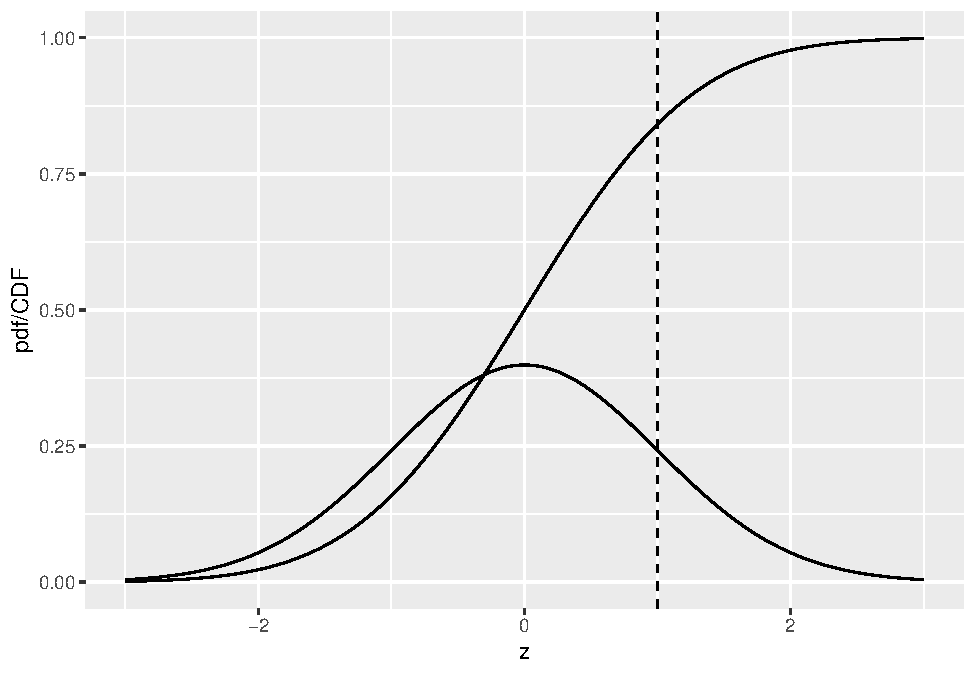
\includegraphics{03-modeling-binary-task_files/figure-latex/binaryTask-plots1-1.pdf}
\caption{\label{fig:binaryTask-plots1}pdf-CDF plots for unit normal.}
\end{figure}

A related function is the inverse of Eqn. \eqref{eq:binaryTask-Phi}. Suppose the left hand side of Eqn. \eqref{eq:binaryTask-Phi} is denoted \(p\), which is a probability in the range 0 to 1.

\begin{equation} 
p=\Phi\left ( z \right )=\int_{-\infty }^{z}\phi(t)dt
\label{eq:binaryTask-Phi2}
\end{equation}

The inverse of \(\Phi(z)\) is that function which when applied to \(p\) yields the upper limit \(z\) in Eqn. \eqref{eq:binaryTask-Phi}, i.e.,

\begin{equation} 
\Phi^{-1}(p) = z
\label{eq:binaryTask-PhiInvDef}
\end{equation}

Since \(p=\Phi(z)\) it follows that

\begin{equation} 
\Phi(\Phi^{-1}(z))=z
\label{eq:binaryTask-PhiInvDef2}
\end{equation}

This nicely satisfies the property of an inverse function. The inverse function is known in statistical terminology as the quantile function, implemented in \texttt{R} as the \texttt{qnorm()} function. Think of \texttt{pnorm()} as a probability and \texttt{qnorm()} as value on the z-axis.

To summarize, \texttt{norm} implies the unit normal distribution, \texttt{p} denotes a probability distribution function or CDF, \texttt{q} denotes a quantile function and \texttt{d} denotes a density function; this convention is used with all distributions in \texttt{R}.

\begin{Shaded}
\begin{Highlighting}[]
\KeywordTok{qnorm}\NormalTok{(}\FloatTok{0.025}\NormalTok{)}
\CommentTok{\#\textgreater{} [1] {-}1.959964}
\KeywordTok{qnorm}\NormalTok{(}\DecValTok{1}\FloatTok{{-}0.025}\NormalTok{)}
\CommentTok{\#\textgreater{} [1] 1.959964}
\KeywordTok{pnorm}\NormalTok{(}\KeywordTok{qnorm}\NormalTok{(}\FloatTok{0.025}\NormalTok{))}
\CommentTok{\#\textgreater{} [1] 0.025}
\KeywordTok{qnorm}\NormalTok{(}\KeywordTok{pnorm}\NormalTok{(}\OperatorTok{{-}}\FloatTok{1.96}\NormalTok{))}
\CommentTok{\#\textgreater{} [1] {-}1.96}
\end{Highlighting}
\end{Shaded}

The first command \texttt{qnorm(0.025)} demonstrates the identity:

\begin{equation} 
\Phi^{-1}(0.025)=-1.959964
\label{eq:binaryTask-Phi-Inv-alpha-by2}
\end{equation}

The next command \texttt{qnorm(1-0.025)} demonstrates the identity:

\begin{equation} 
\Phi^{-1}(1-0.025)=+1.959964
\label{eq:binaryTask-PhiInv-One-Minus-alphaby2}
\end{equation}

The last two commands demonstrate that \texttt{pnorm} and \texttt{qnorm}, applied in either order, are inverses of each other.

Eqn. \eqref{eq:binaryTask-Phi-Inv-alpha-by2} means that the (rounded) value -1.96 is such that the area under the pdf to the left of this value is 0.025. Similarly, Eqn. \eqref{eq:binaryTask-PhiInv-One-Minus-alphaby2} means that the (rounded) value +1.96 is such that the area under the pdf to the left of this value is 1-0.025 = 0.975. In other words, -1.96 captures, to its left, the 2.5th percentile of the unit-normal distribution, and 1.96 captures, to its left, the 97.5th percentile of the unit-normal distribution, Fig. \ref{fig:binaryTask-shaded-tails}. Since between them they capture 95percent of the unit-normal pdf, these two values can be used to estimate 95percent confidence intervals.

\begin{Shaded}
\begin{Highlighting}[]
\NormalTok{mu \textless{}{-}}\StringTok{ }\DecValTok{0}\NormalTok{;sigma \textless{}{-}}\StringTok{ }\DecValTok{1}
\NormalTok{zeta \textless{}{-}}\StringTok{ }\OperatorTok{{-}}\KeywordTok{qnorm}\NormalTok{(}\FloatTok{0.025}\NormalTok{)}
\NormalTok{step \textless{}{-}}\StringTok{ }\FloatTok{0.1}

\NormalTok{LL\textless{}{-}}\StringTok{ }\DecValTok{{-}3}
\NormalTok{UL \textless{}{-}}\StringTok{ }\NormalTok{mu }\OperatorTok{+}\StringTok{ }\DecValTok{3}\OperatorTok{*}\NormalTok{sigma}

\NormalTok{x.values \textless{}{-}}\StringTok{ }\KeywordTok{seq}\NormalTok{(zeta,UL,step)}
\NormalTok{cord.x \textless{}{-}}\StringTok{ }\KeywordTok{c}\NormalTok{(zeta, x.values,UL) }
\NormalTok{cord.y \textless{}{-}}\StringTok{ }\KeywordTok{c}\NormalTok{(}\DecValTok{0}\NormalTok{,}\KeywordTok{dnorm}\NormalTok{(x.values),}\DecValTok{0}\NormalTok{) }

\NormalTok{z \textless{}{-}}\StringTok{ }\KeywordTok{seq}\NormalTok{(LL, UL, }\DataTypeTok{by =}\NormalTok{ step)}
\NormalTok{curveData \textless{}{-}}\StringTok{ }\KeywordTok{data.frame}\NormalTok{(}\DataTypeTok{z =}\NormalTok{ z, }\DataTypeTok{pdfs =} \KeywordTok{dnorm}\NormalTok{(z))}
\NormalTok{shadeData \textless{}{-}}\StringTok{ }\KeywordTok{data.frame}\NormalTok{(}\DataTypeTok{z =}\NormalTok{ cord.x, }\DataTypeTok{pdfs =}\NormalTok{ cord.y)}
\NormalTok{shadedTails \textless{}{-}}\StringTok{ }\KeywordTok{ggplot}\NormalTok{(}\DataTypeTok{mapping =} \KeywordTok{aes}\NormalTok{(}\DataTypeTok{x =}\NormalTok{ z, }\DataTypeTok{y =}\NormalTok{ pdfs))  }\OperatorTok{+}\StringTok{ }
\StringTok{  }\KeywordTok{geom\_polygon}\NormalTok{(}\DataTypeTok{data =}\NormalTok{ shadeData, }\DataTypeTok{color =} \StringTok{"grey"}\NormalTok{, }\DataTypeTok{fill =} \StringTok{"grey"}\NormalTok{)}

\NormalTok{zeta \textless{}{-}}\StringTok{ }\KeywordTok{qnorm}\NormalTok{(}\FloatTok{0.025}\NormalTok{)}
\NormalTok{x.values \textless{}{-}}\StringTok{ }\KeywordTok{seq}\NormalTok{(LL, zeta,step)}
\NormalTok{cord.x \textless{}{-}}\StringTok{ }\KeywordTok{c}\NormalTok{(LL, x.values,zeta) }
\NormalTok{cord.y \textless{}{-}}\StringTok{ }\KeywordTok{c}\NormalTok{(}\DecValTok{0}\NormalTok{,}\KeywordTok{dnorm}\NormalTok{(x.values),}\DecValTok{0}\NormalTok{) }
\NormalTok{shadeData \textless{}{-}}\StringTok{ }\KeywordTok{data.frame}\NormalTok{(}\DataTypeTok{z =}\NormalTok{ cord.x, }\DataTypeTok{pdfs =}\NormalTok{ cord.y)}
\NormalTok{shadedTails \textless{}{-}}\StringTok{ }\NormalTok{shadedTails }\OperatorTok{+}\StringTok{ }
\StringTok{  }\KeywordTok{geom\_polygon}\NormalTok{(}
    \DataTypeTok{data =}\NormalTok{ shadeData, }\DataTypeTok{color =} \StringTok{"grey"}\NormalTok{, }\DataTypeTok{fill =} \StringTok{"grey"}\NormalTok{) }\OperatorTok{+}\StringTok{ }
\StringTok{  }\KeywordTok{xlab}\NormalTok{(}\DataTypeTok{label =} \StringTok{"z"}\NormalTok{) }
\NormalTok{shadedTails \textless{}{-}}\StringTok{ }\NormalTok{shadedTails }\OperatorTok{+}\StringTok{ }
\StringTok{  }\KeywordTok{geom\_line}\NormalTok{(}\DataTypeTok{data =}\NormalTok{ curveData, }\DataTypeTok{color =} \StringTok{"black"}\NormalTok{)}
\KeywordTok{print}\NormalTok{(shadedTails)}
\end{Highlighting}
\end{Shaded}

\begin{figure}
\centering
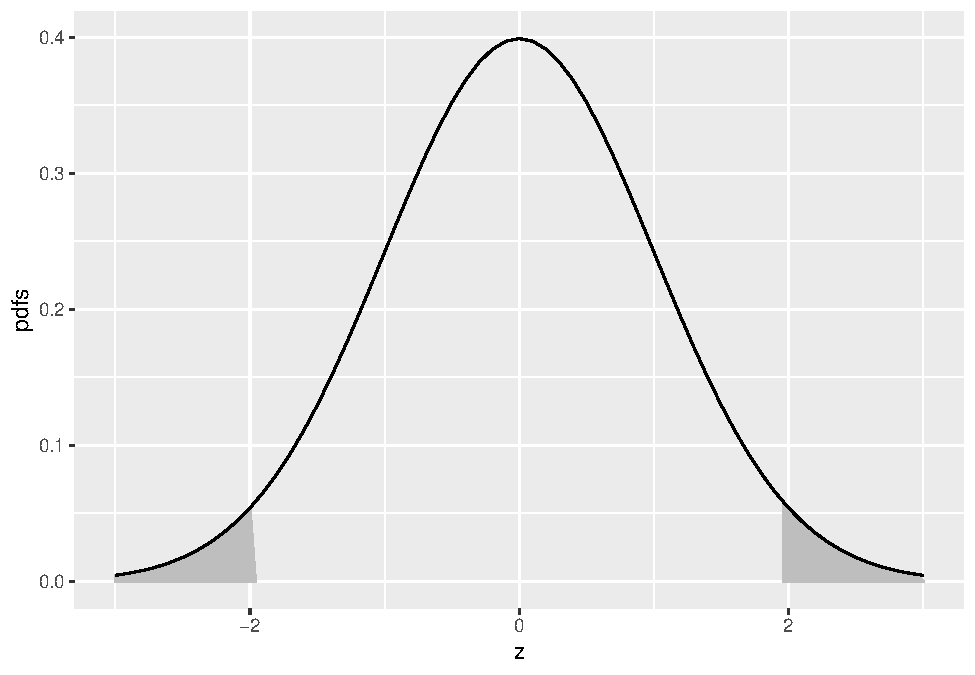
\includegraphics{03-modeling-binary-task_files/figure-latex/binaryTask-shaded-tails-1.pdf}
\caption{\label{fig:binaryTask-shaded-tails}Illustrating that 95percent of the total area under the unit normal pdf is contained in the range \textbar Z\textbar{} \textless{} 1.96, which can be used to construct a 95percent confidence interval for an estimate of a suitably normalized statistic. The area contained in each shaded tail is 2.5percent.}
\end{figure}

\textbf{If one knows that a variable is distributed as a unit-normal random variable, then the observed value minus 1.96 defines the lower limit of its 95percent confidence interval, and the observed value plus 1.96 defines the upper limit of its 95percent confidence interval.}

\hypertarget{analytic-expressions-for-specificity-and-sensitivity}{%
\section{Analytic expressions for specificity and sensitivity}\label{analytic-expressions-for-specificity-and-sensitivity}}

Specificity corresponding to threshold \(\zeta\) is the probability that a Z-sample from a non-diseased case is smaller than \(\zeta\). By definition, this is the CDF corresponding to the threshold \(\zeta\). In other words:

\begin{equation} 
Sp\left ( \zeta \right )=P\left ( Z_{k_11} < \zeta\mid Z_{k_11} \sim N\left ( 0,1 \right )\right ) = \Phi\left ( \zeta \right )
\label{eq:binaryTask-Specificity}
\end{equation}

The expression for sensitivity can be derived tediously by starting with the fact that \(Z_{k_22}\) and then using calculus to obtain the probability that a z-sample for a disease-present case exceeds \(\zeta\). A quicker way is to consider the random variable obtaining by shifting the origin to \(\mu\). A little thought should convince the reader that \(Z_{k_22}-\mu\) must be distributed as \(N(0,1)\). Therefore, the desired probability is (the last step follows from the identity in Eqn. (3.7), with z replaced by \(\zeta-\mu\) :

\begin{equation}
\begin{aligned} 
Se\left ( \zeta \right )\\
=P\left ( Z_{k_22} \geq \zeta\right ) \\
=P\left (\left ( Z_{k_22} -\mu  \right ) \geq\left ( \zeta -\mu  \right )\right ) \\
=1-P\left (\left ( Z_{k_22} -\mu  \right ) < \left ( \zeta -\mu  \right )\right ) \\
= 1-\Phi\left ( \zeta -\mu \right )
\end{aligned}
\label{eq:binaryTask-Sensitivity1}
\end{equation}

A little thought (based on the definition of the CDF function and the symmetry of the unit-normal pdf function) should convince the reader that:

\begin{equation} 
1-\Phi(\zeta)=-\Phi(\zeta)\\
1-\Phi(\zeta-\mu)=\Phi(\mu-\zeta)
\label{eq:binaryTask-Sensitivity2}
\end{equation}

Instead of carrying the ``1 minus'' around, one can use the more compact notation. Summarizing, the analytical formulae for the specificity and sensitivity for the equal-variance binormal model are:

\begin{equation} 
Sp\left ( \zeta \right ) = \Phi(\zeta)\\
Se\left ( \zeta \right ) = \Phi(\mu-\zeta)
\label{eq:binaryTask-Sensitivity-Specificity}
\end{equation}

In these equations, the threshold \(\zeta\) appears with different signs because specificity is the area under a pdf to the \textbf{left} of a threshold, while sensitivity is the area to the \textbf{right}.

\textbf{As probabilities, both sensitivity and specificity are restricted to the range 0 to 1. The observer's performance could be characterized by specifying sensitivity and specificity, i.e., a pair of numbers. If both sensitivity and specificity of an imaging system are greater than the corresponding values for another system, then the 1st system is unambiguously better than the 2nd. But what if sensitivity is greater for the 1st but specificity is greater for the 2nd? Now the comparison is ambiguous. It is difficult to unambiguously compare two pairs of performance indices. Clearly, a scalar measure is desirable that combines sensitivity and specificity into a single measure of diagnostic performance.}

The parameter \(\mu\) satisfies the requirements of a scalar figure of merit (FOM). Eqn. \eqref{eq:binaryTask-Sensitivity-Specificity} can be solved for \(\mu\) as follows. Inverting the equations yields:

\begin{equation} 
\zeta =\Phi^{-1} \left (Sp\left ( \zeta \right )  \right )\\
\mu - \zeta = \Phi^{-1} \left (Se\left ( \zeta \right )  \right )
\label{eq:binaryTask-SolveForMuZeta}
\end{equation}

Eliminating \(\zeta\) yields:

\begin{equation} 
\mu = \Phi^{-1} \left (Sp\left ( \zeta \right )  \right ) + \Phi^{-1} \left (Se\left ( \zeta \right )  \right )
\label{eq:binaryTask-SolveForMu}
\end{equation}

This is a useful relation, as it converts a \emph{pair} of numbers that is hard to compare between two modalities, in the sense described above, into a \emph{single} FOM. Now it is almost trivial to compare two modalities: the one with the higher \(\mu\) wins. In reality, the comparison is not trivial since like sensitivity and specificity, \(\mu\) has to be estimated from a finite dataset and is therefore subject to sampling variability.

\begin{Shaded}
\begin{Highlighting}[]
\KeywordTok{options}\NormalTok{(}\DataTypeTok{digits=}\DecValTok{3}\NormalTok{)}
\NormalTok{mu \textless{}{-}}\StringTok{ }\DecValTok{3}\NormalTok{;sigma \textless{}{-}}\StringTok{ }\DecValTok{1}
\NormalTok{zeta \textless{}{-}}\StringTok{ }\DecValTok{1}
\NormalTok{step \textless{}{-}}\StringTok{ }\FloatTok{0.1}

\NormalTok{lowerLimit\textless{}{-}}\StringTok{ }\DecValTok{{-}1} \CommentTok{\# lower limit}
\NormalTok{upperLimit \textless{}{-}}\StringTok{ }\NormalTok{mu }\OperatorTok{+}\StringTok{ }\DecValTok{3}\OperatorTok{*}\NormalTok{sigma }\CommentTok{\# upper limit}

\NormalTok{z \textless{}{-}}\StringTok{ }\KeywordTok{seq}\NormalTok{(lowerLimit, upperLimit, }\DataTypeTok{by =}\NormalTok{ step)}
\NormalTok{pdfs \textless{}{-}}\StringTok{ }\KeywordTok{dnorm}\NormalTok{(z)}
\NormalTok{seqNor \textless{}{-}}\StringTok{ }\KeywordTok{seq}\NormalTok{(zeta,upperLimit,step)}
\NormalTok{cord.x \textless{}{-}}\StringTok{ }\KeywordTok{c}\NormalTok{(zeta, seqNor,upperLimit) }
\CommentTok{\# need two y{-}coords at each end point of range; }
\CommentTok{\# one at zero and one at value of function}
\NormalTok{cord.y \textless{}{-}}\StringTok{ }\KeywordTok{c}\NormalTok{(}\DecValTok{0}\NormalTok{,}\KeywordTok{dnorm}\NormalTok{(seqNor),}\DecValTok{0}\NormalTok{) }
\NormalTok{curveData \textless{}{-}}\StringTok{ }\KeywordTok{data.frame}\NormalTok{(}\DataTypeTok{z =}\NormalTok{ z, }\DataTypeTok{pdfs =}\NormalTok{ pdfs)}
\NormalTok{shadeData \textless{}{-}}\StringTok{ }\KeywordTok{data.frame}\NormalTok{(}\DataTypeTok{z =}\NormalTok{ cord.x, }\DataTypeTok{pdfs =}\NormalTok{ cord.y)}
\NormalTok{shadedPlots \textless{}{-}}\StringTok{ }\KeywordTok{ggplot}\NormalTok{(}\DataTypeTok{mapping =} \KeywordTok{aes}\NormalTok{(}\DataTypeTok{x =}\NormalTok{ z, }\DataTypeTok{y =}\NormalTok{ pdfs)) }\OperatorTok{+}\StringTok{ }
\StringTok{  }\KeywordTok{geom\_line}\NormalTok{(}\DataTypeTok{data =}\NormalTok{ curveData, }\DataTypeTok{color =} \StringTok{"blue"}\NormalTok{) }\OperatorTok{+}\StringTok{ }
\StringTok{  }\KeywordTok{geom\_polygon}\NormalTok{(}\DataTypeTok{data =}\NormalTok{ shadeData, }\DataTypeTok{color =} \StringTok{"blue"}\NormalTok{, }\DataTypeTok{fill =} \StringTok{"blue"}\NormalTok{)}

\NormalTok{crossing \textless{}{-}}\StringTok{ }\KeywordTok{uniroot}\NormalTok{(}\ControlFlowTok{function}\NormalTok{(x) }\KeywordTok{dnorm}\NormalTok{(x) }\OperatorTok{{-}}\StringTok{ }\KeywordTok{dnorm}\NormalTok{(x,mu,sigma), }
                    \DataTypeTok{lower =} \DecValTok{0}\NormalTok{, }\DataTypeTok{upper =} \DecValTok{3}\NormalTok{)}\OperatorTok{$}\NormalTok{root}
\NormalTok{crossing \textless{}{-}}\StringTok{ }\KeywordTok{max}\NormalTok{(}\KeywordTok{c}\NormalTok{(zeta, crossing))}
\NormalTok{seqAbn \textless{}{-}}\StringTok{ }\KeywordTok{seq}\NormalTok{(crossing,upperLimit,step)}
\NormalTok{cord.x \textless{}{-}}\StringTok{ }\KeywordTok{c}\NormalTok{(seqAbn, }\KeywordTok{rev}\NormalTok{(seqAbn))}
\CommentTok{\# reason for reverse }
\CommentTok{\# we want to explicitly define the polygon}
\CommentTok{\# we dont want R to close it }

\NormalTok{cord.y \textless{}{-}}\StringTok{ }\KeywordTok{c}\NormalTok{()}
\ControlFlowTok{for}\NormalTok{ (i }\ControlFlowTok{in} \KeywordTok{seq}\NormalTok{(}\DecValTok{1}\NormalTok{,}\KeywordTok{length}\NormalTok{(cord.x)}\OperatorTok{/}\DecValTok{2}\NormalTok{)) \{}
\NormalTok{  cord.y \textless{}{-}}\StringTok{ }\KeywordTok{c}\NormalTok{(cord.y,}\KeywordTok{dnorm}\NormalTok{(cord.x[i],mu, sigma))}
\NormalTok{\}}
\ControlFlowTok{for}\NormalTok{ (i }\ControlFlowTok{in} \KeywordTok{seq}\NormalTok{(}\DecValTok{1}\NormalTok{,}\KeywordTok{length}\NormalTok{(cord.x)}\OperatorTok{/}\DecValTok{2}\NormalTok{)) \{}
\NormalTok{  cord.y \textless{}{-}}\StringTok{ }\KeywordTok{c}\NormalTok{(cord.y,}\KeywordTok{dnorm}\NormalTok{(cord.x[}\KeywordTok{length}\NormalTok{(cord.x)}\OperatorTok{/}\DecValTok{2}\OperatorTok{+}\NormalTok{i]))}
\NormalTok{\}}
\NormalTok{pdfs \textless{}{-}}\StringTok{ }\KeywordTok{dnorm}\NormalTok{(z, mu, sigma)}
\NormalTok{curveData \textless{}{-}}\StringTok{ }\KeywordTok{data.frame}\NormalTok{(}\DataTypeTok{z =}\NormalTok{ z, }\DataTypeTok{pdfs =}\NormalTok{ pdfs)}
\NormalTok{shadeData \textless{}{-}}\StringTok{ }\KeywordTok{data.frame}\NormalTok{(}\DataTypeTok{z =}\NormalTok{ cord.x, }\DataTypeTok{pdfs =}\NormalTok{ cord.y)}
\NormalTok{shadedPlots \textless{}{-}}\StringTok{ }\NormalTok{shadedPlots }\OperatorTok{+}\StringTok{ }
\StringTok{  }\KeywordTok{geom\_line}\NormalTok{(}\DataTypeTok{data =}\NormalTok{ curveData, }\DataTypeTok{color =} \StringTok{"red"}\NormalTok{) }\OperatorTok{+}\StringTok{ }
\StringTok{  }\KeywordTok{geom\_polygon}\NormalTok{(}\DataTypeTok{data =}\NormalTok{ shadeData, }\DataTypeTok{color =} \StringTok{"red"}\NormalTok{, }\DataTypeTok{fill =} \StringTok{"red"}\NormalTok{)}
\NormalTok{seqAbn \textless{}{-}}\StringTok{ }\KeywordTok{seq}\NormalTok{(zeta,upperLimit,step)}
\ControlFlowTok{for}\NormalTok{ (i }\ControlFlowTok{in}\NormalTok{ seqAbn) \{}
  \CommentTok{\# define xs and ys of two points, separated only along y{-}axis}
\NormalTok{  vlineData \textless{}{-}}\StringTok{ }\KeywordTok{data.frame}\NormalTok{(}\DataTypeTok{x1 =}\NormalTok{ i, }
                          \DataTypeTok{x2 =}\NormalTok{ i, }
                          \DataTypeTok{y1 =} \DecValTok{0}\NormalTok{, }
                          \DataTypeTok{y2 =} \KeywordTok{dnorm}\NormalTok{(i, mu, sigma))}
  \CommentTok{\# draw vertical line between them}
\NormalTok{  shadedPlots \textless{}{-}}\StringTok{ }\NormalTok{shadedPlots }\OperatorTok{+}\StringTok{ }
\StringTok{    }\KeywordTok{geom\_segment}\NormalTok{(}\KeywordTok{aes}\NormalTok{(}\DataTypeTok{x =}\NormalTok{ x1, }\DataTypeTok{xend =}\NormalTok{ x2, }\DataTypeTok{y =}\NormalTok{ y1, }\DataTypeTok{yend =}\NormalTok{ y2), }
                 \DataTypeTok{data =}\NormalTok{ vlineData, }\DataTypeTok{color =} \StringTok{"red"}\NormalTok{)}
\NormalTok{\}}
\NormalTok{shadedPlots \textless{}{-}}\StringTok{ }\NormalTok{shadedPlots }\OperatorTok{+}\StringTok{ }\KeywordTok{xlab}\NormalTok{(}\DataTypeTok{label =} \StringTok{"z{-}sample"}\NormalTok{)}
\KeywordTok{print}\NormalTok{(shadedPlots)}
\end{Highlighting}
\end{Shaded}

\begin{figure}
\centering
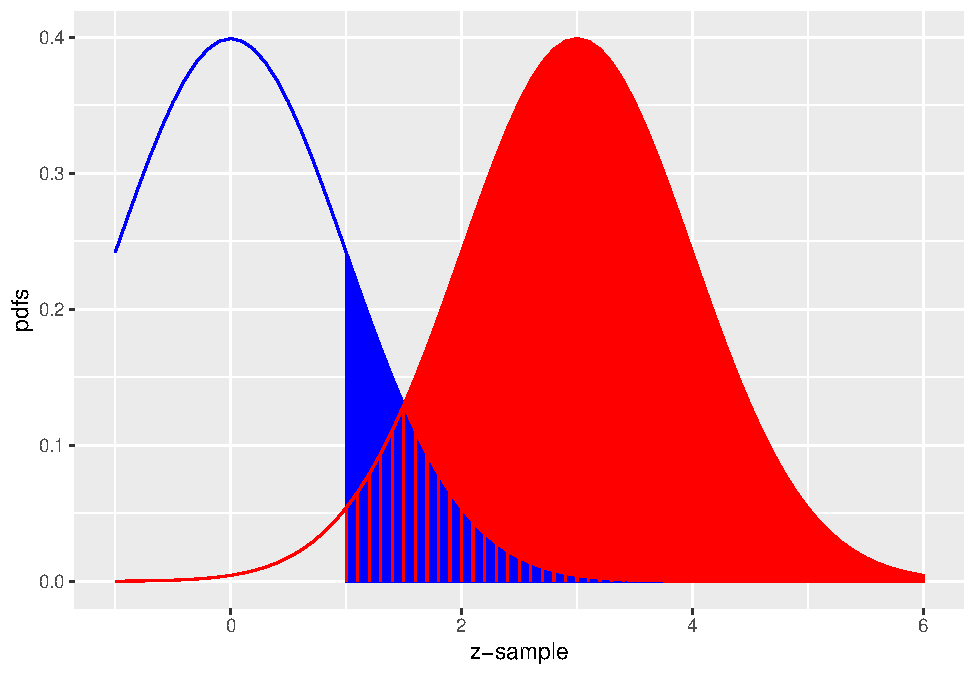
\includegraphics{03-modeling-binary-task_files/figure-latex/binaryTask-shaded-plots-1.pdf}
\caption{\label{fig:binaryTask-shaded-plots}The equal-variance binormal model for mu = 3 and zeta = 1; the blue curve, centered at zero, corresponds to the pdf of non-diseased cases and the red one, centered at mu = 3, corresponds to the pdf of diseased cases. The left edge of the blue shaded region represents the threshold zeta, currently set at unity. The red shaded area, including the common portion with the vertical red lines, is sensitivity. The blue shaded area including the common portion with the vertical red lines is 1-specificity.}
\end{figure}

Fig. \ref{fig:binaryTask-shaded-plots} shows the equal-variance binormal model for \(\mu = 3\) and \(\zeta = 1\). The blue-shaded area, including the ``common'' portion with the vertical red lines, is the probability that a z-sample from a non-diseased case exceeds \(\zeta = 1\), which is the complement of specificity, i.e., it is false positive fraction, which is 1 - \texttt{pnorm(1)} = 0.159. The red shaded area, including the ``common'' portion with the vertical red lines, is the probability that a z-sample from a diseased case exceeds \(\zeta = 1\), which is sensitivity or true positive fraction, which is \texttt{pnorm(3-1)}= 0.977.

Demonstrated next are these concepts using R examples.

\hypertarget{demonstration-of-the-concepts-of-sensitivity-and-specificity}{%
\section{Demonstration of the concepts of sensitivity and specificity}\label{demonstration-of-the-concepts-of-sensitivity-and-specificity}}

\hypertarget{estimating-mu-from-a-finite-sample}{%
\subsection{Estimating mu from a finite sample}\label{estimating-mu-from-a-finite-sample}}

The following code simulates 9 non-diseased and 11 diseased cases. The \(\mu\) parameter is 1.5 and \(\zeta\) is \(\mu/2\). Shown are the calculations of sensitivity and specificity and the value of estimated \(\mu\).

\begin{Shaded}
\begin{Highlighting}[]
\NormalTok{mu \textless{}{-}}\StringTok{ }\FloatTok{1.5}
\NormalTok{zeta \textless{}{-}}\StringTok{ }\NormalTok{mu}\OperatorTok{/}\DecValTok{2}
\NormalTok{seed \textless{}{-}}\StringTok{ }\DecValTok{100} \CommentTok{\# line 4}
\NormalTok{K1 \textless{}{-}}\StringTok{ }\DecValTok{9}
\NormalTok{K2 \textless{}{-}}\StringTok{ }\DecValTok{11}
\NormalTok{ds \textless{}{-}}\StringTok{ }\KeywordTok{simulateDataset}\NormalTok{(K1, K2, mu, zeta, seed)}

\KeywordTok{cat}\NormalTok{(}\StringTok{"seed = "}\NormalTok{, seed, }
    \StringTok{"}\CharTok{\textbackslash{}n}\StringTok{K1 = "}\NormalTok{, K1, }
    \StringTok{"}\CharTok{\textbackslash{}n}\StringTok{K2 = "}\NormalTok{, K2, }
    \StringTok{"}\CharTok{\textbackslash{}n}\StringTok{Specificity = "}\NormalTok{, ds}\OperatorTok{$}\NormalTok{Sp, }
    \StringTok{"}\CharTok{\textbackslash{}n}\StringTok{Sensitivity = "}\NormalTok{, ds}\OperatorTok{$}\NormalTok{Se, }
    \StringTok{"}\CharTok{\textbackslash{}n}\StringTok{Est. of mu = "}\NormalTok{, ds}\OperatorTok{$}\NormalTok{mu, }\StringTok{"}\CharTok{\textbackslash{}n}\StringTok{"}\NormalTok{)}
\CommentTok{\#\textgreater{} seed =  100 }
\CommentTok{\#\textgreater{} K1 =  9 }
\CommentTok{\#\textgreater{} K2 =  11 }
\CommentTok{\#\textgreater{} Specificity =  0.889 }
\CommentTok{\#\textgreater{} Sensitivity =  0.909 }
\CommentTok{\#\textgreater{} Est. of mu =  2.56}
\end{Highlighting}
\end{Shaded}

Since this is a finite sample, the estimate of \(\mu\) is not exactly equal to the true value. In fact, all of the estimates, sensitivity, specificity and \(\mu\) are subject to sampling variability.

\hypertarget{changing-the-seed-variable-case-sampling-variability}{%
\subsection{Changing the seed variable: case-sampling variability}\label{changing-the-seed-variable-case-sampling-variability}}

No matter how many times one runs the above code, one always sees the same output shown above. This is because at line 4 one sets the \texttt{seed} of the random number generator to a fixed value, namely 100. This is like having a perfectly reproducible reader repeatedly interpreting the same cases -- one always gets the same results. Change the \texttt{seed} to 101. One should see:

\begin{Shaded}
\begin{Highlighting}[]
\NormalTok{seed \textless{}{-}}\StringTok{ }\DecValTok{101} \CommentTok{\# change}
\NormalTok{ds \textless{}{-}}\StringTok{ }\KeywordTok{simulateDataset}\NormalTok{(K1, K2, mu, zeta, seed)}

\KeywordTok{cat}\NormalTok{(}\StringTok{"seed = "}\NormalTok{, seed, }
    \StringTok{"}\CharTok{\textbackslash{}n}\StringTok{K1 = "}\NormalTok{, K1, }
    \StringTok{"}\CharTok{\textbackslash{}n}\StringTok{K2 = "}\NormalTok{, K2, }
    \StringTok{"}\CharTok{\textbackslash{}n}\StringTok{Specificity = "}\NormalTok{, ds}\OperatorTok{$}\NormalTok{Sp, }
    \StringTok{"}\CharTok{\textbackslash{}n}\StringTok{Sensitivity = "}\NormalTok{, ds}\OperatorTok{$}\NormalTok{Se, }
    \StringTok{"}\CharTok{\textbackslash{}n}\StringTok{Est. of mu = "}\NormalTok{, ds}\OperatorTok{$}\NormalTok{mu, }\StringTok{"}\CharTok{\textbackslash{}n}\StringTok{"}\NormalTok{)}
\CommentTok{\#\textgreater{} seed =  101 }
\CommentTok{\#\textgreater{} K1 =  9 }
\CommentTok{\#\textgreater{} K2 =  11 }
\CommentTok{\#\textgreater{} Specificity =  0.778 }
\CommentTok{\#\textgreater{} Sensitivity =  0.545 }
\CommentTok{\#\textgreater{} Est. of mu =  0.879}
\end{Highlighting}
\end{Shaded}

Changing \texttt{seed} is equivalent to sampling a completely new set of patients. This is an example of case sampling variability. The effect is quite large (\texttt{Se} fell from 0.909 to 0.545 and estimated \texttt{mu} fell from 2.56 to 0.879!) because the size of the relevant case set, \(K_2=11\) for sensitivity, is rather small, leading to large variability.

\hypertarget{increasing-the-numbers-of-cases}{%
\subsection{Increasing the numbers of cases}\label{increasing-the-numbers-of-cases}}

Here we increase \(K_1\) and \(K_2\), by a factor of 10 each, and return the \texttt{seed} to 100.

\begin{Shaded}
\begin{Highlighting}[]
\NormalTok{K1 \textless{}{-}}\StringTok{ }\DecValTok{90} \CommentTok{\# change}
\NormalTok{K2 \textless{}{-}}\StringTok{ }\DecValTok{110} \CommentTok{\# change}
\NormalTok{seed \textless{}{-}}\StringTok{ }\DecValTok{100} \CommentTok{\# change}
\NormalTok{ds \textless{}{-}}\StringTok{ }\KeywordTok{simulateDataset}\NormalTok{(K1, K2, mu, zeta, seed)}

\KeywordTok{cat}\NormalTok{(}\StringTok{"seed = "}\NormalTok{, seed, }
    \StringTok{"}\CharTok{\textbackslash{}n}\StringTok{K1 = "}\NormalTok{, K1, }
    \StringTok{"}\CharTok{\textbackslash{}n}\StringTok{K2 = "}\NormalTok{, K2, }
    \StringTok{"}\CharTok{\textbackslash{}n}\StringTok{Specificity = "}\NormalTok{, ds}\OperatorTok{$}\NormalTok{Sp, }
    \StringTok{"}\CharTok{\textbackslash{}n}\StringTok{Sensitivity = "}\NormalTok{, ds}\OperatorTok{$}\NormalTok{Se, }
    \StringTok{"}\CharTok{\textbackslash{}n}\StringTok{Est. of mu = "}\NormalTok{, ds}\OperatorTok{$}\NormalTok{mu, }\StringTok{"}\CharTok{\textbackslash{}n}\StringTok{"}\NormalTok{)}
\CommentTok{\#\textgreater{} seed =  100 }
\CommentTok{\#\textgreater{} K1 =  90 }
\CommentTok{\#\textgreater{} K2 =  110 }
\CommentTok{\#\textgreater{} Specificity =  0.778 }
\CommentTok{\#\textgreater{} Sensitivity =  0.836 }
\CommentTok{\#\textgreater{} Est. of mu =  1.74}
\end{Highlighting}
\end{Shaded}

Next we change \texttt{seed} to 101.

\begin{Shaded}
\begin{Highlighting}[]
\NormalTok{seed \textless{}{-}}\StringTok{ }\DecValTok{101} \CommentTok{\# change}
\NormalTok{ds \textless{}{-}}\StringTok{ }\KeywordTok{simulateDataset}\NormalTok{(K1, K2, mu, zeta, seed)}

\KeywordTok{cat}\NormalTok{(}\StringTok{"seed = "}\NormalTok{, seed, }
    \StringTok{"}\CharTok{\textbackslash{}n}\StringTok{K1 = "}\NormalTok{, K1, }
    \StringTok{"}\CharTok{\textbackslash{}n}\StringTok{K2 = "}\NormalTok{, K2, }
    \StringTok{"}\CharTok{\textbackslash{}n}\StringTok{Specificity = "}\NormalTok{, ds}\OperatorTok{$}\NormalTok{Sp, }
    \StringTok{"}\CharTok{\textbackslash{}n}\StringTok{Sensitivity = "}\NormalTok{, ds}\OperatorTok{$}\NormalTok{Se, }
    \StringTok{"}\CharTok{\textbackslash{}n}\StringTok{Est. of mu = "}\NormalTok{, ds}\OperatorTok{$}\NormalTok{mu, }\StringTok{"}\CharTok{\textbackslash{}n}\StringTok{"}\NormalTok{)}
\CommentTok{\#\textgreater{} seed =  101 }
\CommentTok{\#\textgreater{} K1 =  90 }
\CommentTok{\#\textgreater{} K2 =  110 }
\CommentTok{\#\textgreater{} Specificity =  0.811 }
\CommentTok{\#\textgreater{} Sensitivity =  0.755 }
\CommentTok{\#\textgreater{} Est. of mu =  1.57}
\end{Highlighting}
\end{Shaded}

Notice that now the values are less sensitive to seed. Table \ref{tab:binaryTask0SeSpMuvsCaseSizeSeed} illustrates this trend with ever increasing sample sizes (the reader should confirm the listed values).

\begin{Shaded}
\begin{Highlighting}[]
\NormalTok{results \textless{}{-}}\StringTok{ }\KeywordTok{array}\NormalTok{(}\DataTypeTok{dim =} \KeywordTok{c}\NormalTok{(}\DecValTok{9}\NormalTok{,}\DecValTok{6}\NormalTok{))}
\NormalTok{mu \textless{}{-}}\StringTok{ }\FloatTok{1.5}
\NormalTok{zeta \textless{}{-}}\StringTok{ }\NormalTok{mu}\OperatorTok{/}\DecValTok{2}
\NormalTok{results[}\DecValTok{9}\NormalTok{,] \textless{}{-}}\StringTok{ }\KeywordTok{c}\NormalTok{(}\OtherTok{Inf}\NormalTok{, }\OtherTok{Inf}\NormalTok{, }\OtherTok{NA}\NormalTok{, }\KeywordTok{pnorm}\NormalTok{(zeta), }\KeywordTok{pnorm}\NormalTok{(mu}\OperatorTok{{-}}\NormalTok{zeta), mu)}
\NormalTok{K1\_arr \textless{}{-}}\StringTok{ }\KeywordTok{c}\NormalTok{(}\DecValTok{9}\NormalTok{, }\DecValTok{9}\NormalTok{, }\DecValTok{90}\NormalTok{, }\DecValTok{90}\NormalTok{, }\DecValTok{900}\NormalTok{, }\DecValTok{900}\NormalTok{, }\DecValTok{9000}\NormalTok{, }\DecValTok{9000}\NormalTok{, }\OtherTok{NA}\NormalTok{)}
\NormalTok{K2\_arr \textless{}{-}}\StringTok{ }\KeywordTok{c}\NormalTok{(}\DecValTok{11}\NormalTok{, }\DecValTok{11}\NormalTok{, }\DecValTok{110}\NormalTok{, }\DecValTok{110}\NormalTok{, }\DecValTok{1100}\NormalTok{, }\DecValTok{1100}\NormalTok{, }\DecValTok{11000}\NormalTok{, }\DecValTok{11000}\NormalTok{, }\OtherTok{NA}\NormalTok{)}
\NormalTok{seed\_arr \textless{}{-}}\StringTok{ }\KeywordTok{c}\NormalTok{(}\DecValTok{100}\NormalTok{,}\DecValTok{101}\NormalTok{,}\DecValTok{100}\NormalTok{,}\DecValTok{101}\NormalTok{,}\DecValTok{100}\NormalTok{,}\DecValTok{101}\NormalTok{,}\DecValTok{100}\NormalTok{,}\DecValTok{101}\NormalTok{,}\OtherTok{NA}\NormalTok{)}
\ControlFlowTok{for}\NormalTok{ (i }\ControlFlowTok{in} \DecValTok{1}\OperatorTok{:}\DecValTok{8}\NormalTok{) \{}
\NormalTok{  ds \textless{}{-}}\StringTok{ }\KeywordTok{simulateDataset}\NormalTok{(K1\_arr[i], K2\_arr[i], mu, zeta, seed\_arr[i])}
\NormalTok{  results[i,] \textless{}{-}}\StringTok{ }\KeywordTok{c}\NormalTok{(K1\_arr[i], K2\_arr[i], seed\_arr[i], ds}\OperatorTok{$}\NormalTok{Sp, ds}\OperatorTok{$}\NormalTok{Se, ds}\OperatorTok{$}\NormalTok{mu)}
\NormalTok{\}}
\NormalTok{df \textless{}{-}}\StringTok{ }\KeywordTok{as.data.frame}\NormalTok{(results)}
\KeywordTok{colnames}\NormalTok{(df) \textless{}{-}}\StringTok{ }\KeywordTok{c}\NormalTok{(}\StringTok{"K1"}\NormalTok{,}\StringTok{"K2"}\NormalTok{,}\StringTok{"seed"}\NormalTok{,}\StringTok{"Se"}\NormalTok{,}\StringTok{"Sp"}\NormalTok{,}\StringTok{"mu"}\NormalTok{)}
\end{Highlighting}
\end{Shaded}

\begin{table}

\caption{\label{tab:binaryTask0SeSpMuvsCaseSizeSeed}Effect of sample size and seed on estimates of sensitivity, specificity and the mu-parameter.}
\centering
\begin{tabular}[t]{r|r|r|r|r|r}
\hline
K1 & K2 & seed & Se & Sp & mu\\
\hline
9 & 11 & 100 & 0.889 & 0.909 & 2.556\\
\hline
9 & 11 & 101 & 0.778 & 0.545 & 0.879\\
\hline
90 & 110 & 100 & 0.778 & 0.836 & 1.744\\
\hline
90 & 110 & 101 & 0.811 & 0.755 & 1.571\\
\hline
900 & 1100 & 100 & 0.764 & 0.761 & 1.430\\
\hline
900 & 1100 & 101 & 0.807 & 0.759 & 1.569\\
\hline
9000 & 11000 & 100 & 0.774 & 0.772 & 1.496\\
\hline
9000 & 11000 & 101 & 0.771 & 0.775 & 1.498\\
\hline
Inf & Inf & NA & 0.773 & 0.773 & 1.500\\
\hline
\end{tabular}
\end{table}

As the numbers of cases increase, the sensitivity and specificity converge to a common value, around 0.773 and the estimate of the separation parameter converges to the known value.

\begin{Shaded}
\begin{Highlighting}[]
\KeywordTok{pnorm}\NormalTok{(}\FloatTok{0.75}\NormalTok{) }\CommentTok{\# example 1}
\CommentTok{\#\textgreater{} [1] 0.773}
\DecValTok{2}\OperatorTok{*}\KeywordTok{qnorm}\NormalTok{(}\KeywordTok{pnorm}\NormalTok{(zeta)) }\CommentTok{\# example 2}
\CommentTok{\#\textgreater{} [1] 1.5}
\end{Highlighting}
\end{Shaded}

Because the threshold is halfway between the two distributions, as in this example, sensitivity and specificity are identical. In words, with two unit variance distributions separated by 1.5, the area under the diseased distribution (centered at 1.5) above 0.75, namely sensitivity, equals the area under the non-diseased distribution (centered at zero) below 0.75, namely specificity, and the common value is \(\Phi(0.75)= 0.773\), yielding the last row of Table \ref{tab:binaryTask0SeSpMuvsCaseSizeSeed}, and example 1 in the above code snippet. Example 2 in the above code snippet illustrates Eqn. \eqref{eq:binaryTask-SolveForMu}. The factor of two arises since in this example sensitivity and specificity are identical.

From Table \ref{tab:binaryTask0SeSpMuvsCaseSizeSeed}, for the same numbers of cases but different seeds, comparing pairs of sensitivity and specificity values is more difficult as two pairs of numbers (i.e., four numbers) are involved. Comparing a single pair of \(\mu\) values is easier as only two numbers are involved. The tendency of the pairs to become independent of case sample is discernible with fewer cases with \(\mu\), around 90/110 cases, than with sensitivity and specificity pairs. The numbers in the table might appear disheartening in terms of the implied numbers of cases needed to detect a difference in specificity. Even with 200 cases, the difference in specificity for two seed values is 0.081, which is actually a large effect considering that the scale extends from 0 to 1.0. A similar comment applies to differences in sensitivity. The situation is not quite that bad. One uses an area measure that combines sensitivity and specificity yielding less variability in the combined measure. One uses the ratings paradigm, which is more efficient than the binary one used in this chapter. Finally, one takes advantage of correlations that exist between the interpretations in matched-case matched-reader interpretations in two modalities that tend to decrease variability in the AUC-difference even further (most applications of ROC methods involved detecting differences in AUCs not absolute values).

\hypertarget{inverse-variation-of-sensitivity-and-specificity-and-the-need-for-a-single-fom}{%
\section{Inverse variation of sensitivity and specificity and the need for a single FOM}\label{inverse-variation-of-sensitivity-and-specificity-and-the-need-for-a-single-fom}}

The variation of sensitivity and specificity is modeled in the binormal model by the threshold parameter \(\zeta\). From Eqn. \eqref{eq:binaryTask-Specificity}, specificity at threshold \(\zeta\) is \(\Phi(\zeta)\) and the corresponding expression for sensitivity is \(\Phi(\mu-\zeta)\). Since the threshold \(\zeta\) appears with a minus sign, the dependence of sensitivity on \(\zeta\) will be the opposite of the corresponding dependence of specificity on \(\zeta\). In Fig. \ref{fig:binaryTask-shaded-plots}, the left edge of the blue shaded region represents the threshold \(\zeta = 1\). As \(\zeta = 1\) is moved towards the left, specificity decreases but sensitivity increases. Specificity decreases because less of the non-diseased distribution lies to the left of the new threshold, in other words fewer non-diseased cases are correctly diagnosed as non-diseased. Sensitivity increases because more of the diseased distribution lies to the right of the new threshold, in other words more diseased cases are correctly diagnosed as diseased. If an observer has higher sensitivity than another observer, but lower specificity, it is difficult to unambiguously compare them. It is not impossible \citep{RN2637}. The unambiguous comparison is difficult for the following reason. Assuming the second observer can be coaxed into adopting a lower threshold, thereby decreasing specificity to match that of the first observer, then it is possible that the second observer's sensitivity, formerly smaller, could now be greater than that of the first observer. A single figure of merit is desirable to the sensitivity - specificity analysis. It is possible to leverage the inverse variation of sensitivity and specificity by combing them into a single scalar measure, as was done with the \(\mu\) parameter in the previous section, Eqn. \eqref{eq:binaryTask-SolveForMu}. An equivalent way is by using the area under the ROC plot, discussed next.

\hypertarget{the-roc-curve}{%
\section{The ROC curve}\label{the-roc-curve}}

The receiver operating characteristic (ROC) is defined as the plot of sensitivity (y-axis) vs.~1-specificity (x-axis). Equivalently, it is the plot of TPF (y-axis) vs.~FPF (x-axis). From Eqn. \eqref{eq:binaryTask-Sensitivity-Specificity} it follows that:

\begin{equation} 
\begin{aligned} 
FPF\left ( \zeta \right ) &= 1 - Sp\left ( \zeta \right ) \\
&=\Phi\left ( -\zeta \right )\\
\\
TPF\left ( \zeta \right ) &= Se\left ( \zeta \right ) \\
&=\Phi\left (\mu -\zeta \right )\\ 
\end{aligned} 
\label{eq:binaryTask-FPF-TPF}
\end{equation}

Specifying \(\zeta\) selects a particular operating point on this plot and varying \(\zeta\) from \(+\infty\) to \(-\infty\) causes the operating point to trace out the ROC curve from the origin (0,0) to (1,1). Specifically, as \(\zeta\) is decreased from \(+\infty\) to \(-\infty\), the operating point rises from the origin (0,0) to the end-point (1,1). In general, as \(\zeta\) increases, the operating point moves down the curve, and conversely, as \(\zeta\) decreases the operating point moves up the curve. The operating point \(O(\zeta|\mu)\) for the equal variance binormal model is (the notation assumes the \(\mu\) parameter is fixed and \(\zeta\) is varied by the observer in response to interpretation conditions):

\begin{equation} 
O\left ( \zeta \mid \mu \right ) = \left ( \Phi(-\zeta), \Phi(\mu-\zeta) \right ) \\
\label{eq:binaryTask-OpPt}
\end{equation}

The operating point predicted by the above equation lies exactly on the theoretical ROC curve. This condition can only be achieved with very large numbers of cases, so that sampling variability is very small. In practice, with finite datasets, the operating point will almost never be exactly on the theoretical curve.

\textbf{The ROC curve is the locus of the operating point for fixed \(\mu\) and variable \(\zeta\). Fig. \ref{fig:binaryTask-RocCurvesEqVarModel} shows examples of equal-variance binormal model ROC curves for different values of \(\mu\). Each curve is labeled with the corresponding value of \(\mu\). Each has the property that TPF is a monotonically increasing function of FPF and the slope decreases monotonically as the operating point moves up the curve. As \(\mu\) increases the curves get progressively upward-left shifted, approaching the top-left corner of the ROC plot. In the limit \(\mu = \infty\) the curve degenerates into two line segments, a vertical one connecting the origin to (0,1) and a horizontal one connecting (0,1) to (1,1) -- the ROC plot for a perfect observer.}

\begin{Shaded}
\begin{Highlighting}[]
\NormalTok{mu \textless{}{-}}\StringTok{ }\DecValTok{0}\NormalTok{;zeta \textless{}{-}}\StringTok{ }\KeywordTok{seq}\NormalTok{(}\OperatorTok{{-}}\DecValTok{5}\NormalTok{, mu }\OperatorTok{+}\StringTok{ }\DecValTok{5}\NormalTok{, }\FloatTok{0.05}\NormalTok{)}
\NormalTok{FPF \textless{}{-}}\StringTok{ }\KeywordTok{pnorm}\NormalTok{(}\OperatorTok{{-}}\NormalTok{zeta)}
\NormalTok{rocPlot \textless{}{-}}\StringTok{ }\KeywordTok{ggplot}\NormalTok{(}\DataTypeTok{mapping =} \KeywordTok{aes}\NormalTok{(}\DataTypeTok{x =}\NormalTok{ FPF, }\DataTypeTok{y =}\NormalTok{ TPF))}
\ControlFlowTok{for}\NormalTok{ (mu }\ControlFlowTok{in} \DecValTok{0}\OperatorTok{:}\DecValTok{3}\NormalTok{)\{}
\NormalTok{  TPF \textless{}{-}}\StringTok{ }\KeywordTok{pnorm}\NormalTok{(mu}\OperatorTok{{-}}\NormalTok{zeta)}
\NormalTok{  curveData \textless{}{-}}\StringTok{ }\KeywordTok{data.frame}\NormalTok{(}\DataTypeTok{FPF =}\NormalTok{ FPF, }\DataTypeTok{TPF =}\NormalTok{ TPF)}
\NormalTok{  rocPlot \textless{}{-}}\StringTok{ }\NormalTok{rocPlot }\OperatorTok{+}\StringTok{ }
\StringTok{    }\KeywordTok{geom\_line}\NormalTok{(}\DataTypeTok{data =}\NormalTok{ curveData, }\DataTypeTok{size =} \DecValTok{2}\NormalTok{) }\OperatorTok{+}\StringTok{ }
\StringTok{    }\KeywordTok{xlab}\NormalTok{(}\StringTok{"FPF"}\NormalTok{)}\OperatorTok{+}\StringTok{ }\KeywordTok{ylab}\NormalTok{(}\StringTok{"TPF"}\NormalTok{ ) }\OperatorTok{+}\StringTok{ }
\StringTok{    }\KeywordTok{theme}\NormalTok{(}\DataTypeTok{axis.title.y =} \KeywordTok{element\_text}\NormalTok{(}\DataTypeTok{size =} \DecValTok{25}\NormalTok{,}\DataTypeTok{face=}\StringTok{"bold"}\NormalTok{),}
          \DataTypeTok{axis.title.x =} \KeywordTok{element\_text}\NormalTok{(}\DataTypeTok{size =} \DecValTok{30}\NormalTok{,}\DataTypeTok{face=}\StringTok{"bold"}\NormalTok{))  }\OperatorTok{+}
\StringTok{    }\KeywordTok{annotate}\NormalTok{(}\StringTok{"text"}\NormalTok{, }
             \DataTypeTok{x =} \KeywordTok{pnorm}\NormalTok{(}\OperatorTok{{-}}\NormalTok{mu}\OperatorTok{/}\DecValTok{2}\NormalTok{) }\OperatorTok{+}\StringTok{ }\FloatTok{0.07}\NormalTok{, }
             \DataTypeTok{y =} \KeywordTok{pnorm}\NormalTok{(mu}\OperatorTok{/}\DecValTok{2}\NormalTok{), }
             \DataTypeTok{label =} \KeywordTok{paste0}\NormalTok{(}\StringTok{"mu == "}\NormalTok{, mu), }
             \DataTypeTok{parse =} \OtherTok{TRUE}\NormalTok{, }\DataTypeTok{size =} \DecValTok{8}\NormalTok{)}
  \ControlFlowTok{next}
\NormalTok{\}}
\NormalTok{rocPlot \textless{}{-}}\StringTok{ }\NormalTok{rocPlot }\OperatorTok{+}
\StringTok{  }\KeywordTok{scale\_x\_continuous}\NormalTok{(}\DataTypeTok{expand =} \KeywordTok{c}\NormalTok{(}\DecValTok{0}\NormalTok{, }\DecValTok{0}\NormalTok{)) }\OperatorTok{+}\StringTok{ }
\StringTok{  }\KeywordTok{scale\_y\_continuous}\NormalTok{(}\DataTypeTok{expand =} \KeywordTok{c}\NormalTok{(}\DecValTok{0}\NormalTok{, }\DecValTok{0}\NormalTok{))     }

\NormalTok{rocPlot \textless{}{-}}\StringTok{ }\NormalTok{rocPlot }\OperatorTok{+}\StringTok{ }
\StringTok{  }\KeywordTok{geom\_abline}\NormalTok{(}\DataTypeTok{slope =} \DecValTok{{-}1}\NormalTok{, }
              \DataTypeTok{intercept =} \DecValTok{1}\NormalTok{, }
              \DataTypeTok{linetype =} \DecValTok{3}\NormalTok{,}
              \DataTypeTok{size =} \DecValTok{2}\NormalTok{)}
\KeywordTok{print}\NormalTok{(rocPlot)}
\end{Highlighting}
\end{Shaded}

\begin{figure}
\centering
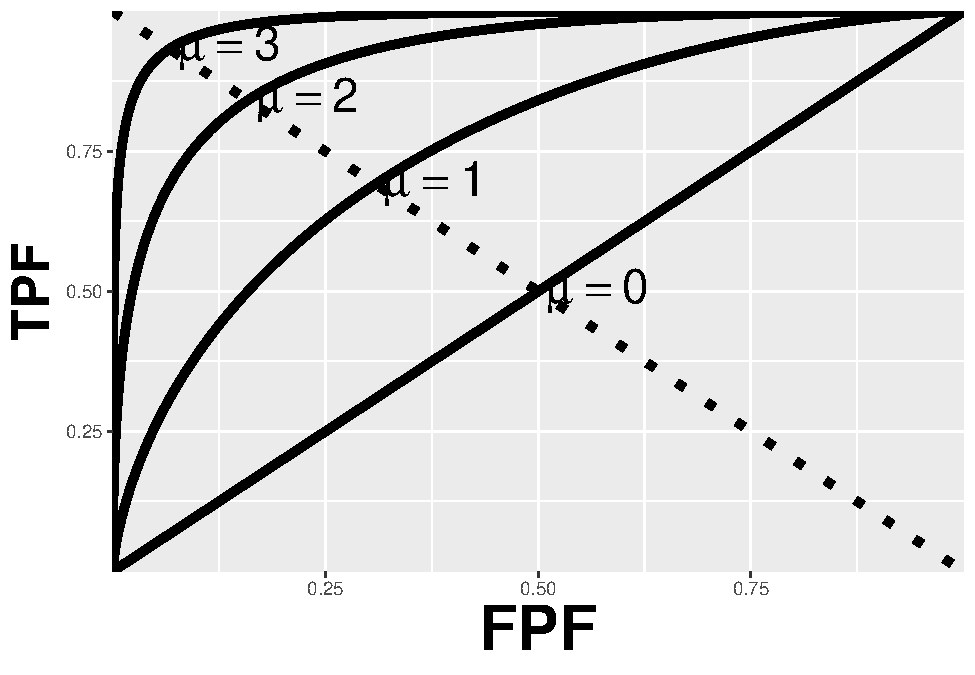
\includegraphics{03-modeling-binary-task_files/figure-latex/binaryTask-RocCurvesEqVarModel-1.pdf}
\caption{\label{fig:binaryTask-RocCurvesEqVarModel}ROC plots predicted by the equal variance binormal model for different values of mu. As mu increases the intersection of the curve with the negative diagonal moves closer to the ideal operating point, (0,1) at which sensitivity and specificity are both equal to unity.}
\end{figure}

\hypertarget{the-chance-diagonal}{%
\subsection{The chance diagonal}\label{the-chance-diagonal}}

In Fig. \ref{fig:binaryTask-RocCurvesEqVarModel} the ROC curve for \(\mu=0\) is the positive diagonal of the ROC plot, termed the chance diagonal. Along this curve \(TPF = FPF\) and the observer's performance is at chance level. In the equal variance binormal model, for \(\mu=0\), the pdf of the diseased distribution is identical to that of the non-diseased distribution: both are centered at the origin. Therefore, no matter the choice of threshold \(\zeta\), \(TPF = FPF\). Setting \(\mu=0\) in Eqn. \eqref{eq:binaryTask-FPF-TPF} yields:

\[TPF\left ( \zeta \right )=FPF\left ( \zeta \right )=\Phi\left ( -\zeta \right )\]
In this special case, the red and blue curves in Fig. \ref{fig:binaryTask-shaded-plots} coincide. The observer is unable to find any difference between the two distributions. This can happen if the cancers are of such low visibility so that diseased cases are indistinguishable from non-diseased ones, or the observer's skill level is so poor that the observer is unable to make use of distinguishing characteristics between diseased and non-diseased cases that do exist, and which experts exploit.

\hypertarget{the-guessing-observer}{%
\subsection{The guessing observer}\label{the-guessing-observer}}

If the cases are indeed impossibly difficult and/or the observer has zero skill at discriminating between them, the observer has no option but to guess. This rarely happens in the clinic, as too much is at stake and this paragraph is intended to make a pedagogical point that the observer can move the operating point along the change diagonal. If there is no special incentive, the observer tosses a coin and if the coin lands head up, the observer states: ``case is diseased'' and otherwise states: ``case is non-diseased''. When this procedure is averaged over many non-diseased and diseased cases, it will result in the operating point (0.5, 0.5). {[}Many cases are assumed as otherwise, due to sampling variability, the operating point will not be on the theoretical ROC curve.{]} To move the operating point downward, e.g., to (0.1, 0.1) the observer randomly selects an integer number between 1 and 10, equivalent to a 10-sided ``coin''. Whenever a one ``shows up'', the observer states ``case is diseased'' and otherwise the observer states ``case is non-diseased''. To move the operating point to (0.2, 0.2) whenever a one or two ``shows up'', the observer states ``case is diseased'' and otherwise the observer states ``case is non-diseased''. One can appreciate that simply by changing the probability of stating ``case is diseased'' the observer can place the operating point anywhere on the chance diagonal, but wherever the operating point is placed, it will satisfy TPF = FPF.

\hypertarget{symmetry-with-respect-to-negative-diagonal}{%
\subsection{Symmetry with respect to negative diagonal}\label{symmetry-with-respect-to-negative-diagonal}}

A characteristic of the ROC curves shown in Fig. \ref{fig:binaryTask-RocCurvesEqVarModel} is that they are symmetric with respect to the negative diagonal, defined as the straight line joining (0,1) and (1,0) which is shown as the dotted straight line in Fig. \ref{fig:binaryTask-RocCurvesEqVarModel}. The symmetry property is due to the equal variance nature of the binormal model and is not true for models considered in later chapters. The intersection between the ROC curve and the negative diagonal corresponds to \(\zeta = \mu/2\), in which case the operating point is:

\begin{equation} 
\begin{aligned} 
FPF\left ( \zeta \right ) &=\Phi\left ( -\mu/2 \right )\\
\\
TPF\left ( \zeta \right ) &=\Phi\left (\mu/2 \right )\\ 
\end{aligned} 
\label{eq:binaryTask-NegDiagIntersection}
\end{equation}

The first equation implies:

\[1-FPF\left ( \zeta \right ) =1-\Phi\left ( -\mu/2 \right )= \Phi\left ( \mu/2 \right )\]
Therefore,

\begin{equation} 
TPF\left ( \zeta \right ) = 1-FPF\left ( \zeta \right )
\label{eq:binaryTask-NegDiagIntersection2}
\end{equation}

This equation describes a straight line with unit intercept and slope equal to minus 1, which is the negative diagonal. Since TPF = sensitivity and FPF = 1- specificity, another way of stating this is that at the intersection with the negative diagonal, sensitivity equals specificity.

\hypertarget{area-under-the-roc-curve}{%
\subsection{Area under the ROC curve}\label{area-under-the-roc-curve}}

The area AUC (abbreviation for area under curve) under the ROC curve suggests itself as a measure of performance that is independent of threshold and therefore circumvents the ambiguity issue of comparing sensitivity/specificity pairs, and has other advantages. It is defined by the following integrals:

\begin{equation} 
\begin{aligned}
A_{z;\sigma = 1} &= \int_{0}^{1}TPF(\zeta)d(FPF(\zeta))\\
&=\int_{0}^{1}FPF(\zeta)d(TPF(\zeta))\\
\end{aligned}
\label{eq:binaryTask-Az-EqVarModel}
\end{equation}

Eqn. \eqref{eq:binaryTask-Az-EqVarModel} has the following equivalent interpretations:

\begin{itemize}
\tightlist
\item
  The first form performs the integration using thin vertical strips, e.g., extending from x to x + dx, where for convenience x is a temporary symbol for FPF. The area can be interpreted as the average TPF over all possible values of FPF.
\item
  The second form performs the integration using thin horizontal strips, e.g., extending from y to y + dy, where for convenience y is a temporary symbol for TPF. The area can be interpreted as the average FPF over all possible values of TPF.
\end{itemize}

By convention, the symbol \(A_z\) is used for the area under the binormal model predicted ROC curve. In Eqn. \eqref{eq:binaryTask-Az-EqVarModel}, the extra subscript \(\sigma = 1\) is necessary to distinguish it from another one corresponding to the unequal variance binormal model to be derived later. It can be shown that:

\begin{equation} 
A_{z;\sigma = 1} = \Phi\left ( \frac{\mu} {\sqrt{2}} \right )
\label{eq:binaryTask-Az-EqVarModel2}
\end{equation}

Since the ROC curve is bounded by the unit square, AUC must be between zero and one. If \(\mu\) is non-negative, the area under the ROC curve must be between 0.5 and 1. The chance diagonal, corresponding to \(\mu = 0\), yields \(A_{z;\sigma = 1} = 0.5\), while the perfect ROC curve, corresponding to infinite yields unit area. Since it is a scalar quantity, AUC can be used to less-ambiguously quantify performance in the ROC task than is possible using sensitivity - specificity pairs.

\hypertarget{properties-of-the-equal-variance-binormal-model-roc-curve}{%
\subsection{Properties of the equal-variance binormal model ROC curve}\label{properties-of-the-equal-variance-binormal-model-roc-curve}}

\begin{enumerate}
\def\labelenumi{\alph{enumi}.}
\tightlist
\item
  The ROC curve is completely contained within the unit square. This follows from the fact that both axes of the plot are probabilities.
\item
  The operating point rises monotonically from (0,0) to (1,1).
\item
  Since \(\mu\) is positive, the slope of the equal-variance binormal model curve at the origin (0,0) is infinite and the slope at (1,1) is zero, and the slope along the curve is always non-negative and decreases monotonically as the operating point moves up the curve.
\item
  AUC is a monotone increasing function of \(\mu\). It varies from 0.5 to 1 as \(\mu\) varies from zero to infinity.
\end{enumerate}

\hypertarget{comments}{%
\subsection{Comments}\label{comments}}

Property (b): since the operating point coordinates can both be expressed in terms of \(\Phi\) functions, which are monotone in their arguments, and in each case the argument appears with a negative sign, it follows that as \(\zeta\) is lowered both TPF and FPF increase. In other words, the operating point corresponding to \(\zeta - d\zeta\) is to the upper right of that corresponding \(\zeta\) to (assuming \(d\zeta > 0\)).

Property (c): The slope of the ROC curve can be derived by differentiation (\(\mu\) is constant):

\begin{equation} 
\left.
\begin{aligned}
\frac{d(TPF)}{d(FPF)}&=\frac{d(\Phi(\mu-\zeta))}{d(\Phi(-\zeta))}\\
&=\frac{\phi(\mu-\zeta)}{\phi(-\zeta)}\\
&=exp(\mu(\zeta-\mu/2)) \propto exp(\mu \zeta)\\
\end{aligned}
\right \}
\label{eq:binaryTask-slopeROC1}
\end{equation}

The above derivation uses the fact that the differential of the CDF function yields the pdf function, i.e.,

\[d\Phi(\zeta)=P\left ( \zeta < Z < \zeta + d \zeta \right ) = \phi(\zeta)d\zeta\]

Since the slope of the ROC curve can be expressed as a power of \(e\), it is always non-negative. Provided \(\mu > 0\), then, in the limit \(\zeta\rightarrow \infty\), the slope at the origin approaches \(\infty\). Eqn. \eqref{eq:binaryTask-slopeROC1} also implies that in the limit \(\zeta\rightarrow -\infty\) the slope of the ROC curve at the end-point (1,1) approaches zero, i.e., the slope is a monotone increasing function of \(\zeta\). As \(\zeta\) decrease from \(+\infty\) to \(-\infty\), the slope decreases monotonically from \(+\infty\) to 0.

Fig. \ref{fig:binaryTask-MainAnalyticalROC} is the ROC curve for the equal-variance binormal model for . The entire curve is defined by . Specifying a particular value of corresponds to specifying a particular point on the ROC curve. In Fig. 3.5 the open circle corresponds to the operating point (0.159, 0.977) defined by = 1; pnorm(-1) = 0.159; pnorm(3-1) = 0.977. The operating point lies exactly on the curve, as this is a predicted operating point.

\begin{Shaded}
\begin{Highlighting}[]
\NormalTok{mu \textless{}{-}}\StringTok{ }\DecValTok{3}\NormalTok{;zeta \textless{}{-}}\StringTok{ }\KeywordTok{seq}\NormalTok{(}\OperatorTok{{-}}\DecValTok{4}\NormalTok{,mu}\OperatorTok{+}\DecValTok{3}\NormalTok{,}\FloatTok{0.05}\NormalTok{)}
\NormalTok{FPF \textless{}{-}}\StringTok{ }\KeywordTok{pnorm}\NormalTok{(}\OperatorTok{{-}}\NormalTok{zeta)}
\NormalTok{TPF \textless{}{-}}\StringTok{ }\KeywordTok{pnorm}\NormalTok{(mu }\OperatorTok{{-}}\NormalTok{zeta) }
\NormalTok{FPF \textless{}{-}}\StringTok{ }\KeywordTok{c}\NormalTok{(}\DecValTok{1}\NormalTok{, FPF, }\DecValTok{0}\NormalTok{);TPF \textless{}{-}}\StringTok{ }\KeywordTok{c}\NormalTok{(}\DecValTok{1}\NormalTok{, TPF, }\DecValTok{0}\NormalTok{)}
\NormalTok{curveData \textless{}{-}}\StringTok{ }\KeywordTok{data.frame}\NormalTok{(}\DataTypeTok{FPF =}\NormalTok{ FPF, }\DataTypeTok{TPF =}\NormalTok{ TPF)}
\NormalTok{OpX \textless{}{-}}\StringTok{ }\KeywordTok{pnorm}\NormalTok{(}\OperatorTok{{-}}\DecValTok{1}\NormalTok{)}
\NormalTok{OpY \textless{}{-}}\StringTok{ }\KeywordTok{pnorm}\NormalTok{(mu}\DecValTok{{-}1}\NormalTok{)}
\NormalTok{pointData \textless{}{-}}\StringTok{ }\KeywordTok{data.frame}\NormalTok{(}\DataTypeTok{FPF =}\NormalTok{ OpX, }\DataTypeTok{TPF =}\NormalTok{ OpY)}
\NormalTok{rocPlot \textless{}{-}}\StringTok{ }\KeywordTok{ggplot}\NormalTok{(}
  \DataTypeTok{mapping =} \KeywordTok{aes}\NormalTok{(}\DataTypeTok{x =}\NormalTok{ FPF, }\DataTypeTok{y =}\NormalTok{ TPF)) }\OperatorTok{+}\StringTok{ }
\StringTok{  }\KeywordTok{xlab}\NormalTok{(}\StringTok{"FPF"}\NormalTok{)}\OperatorTok{+}\StringTok{ }\KeywordTok{ylab}\NormalTok{(}\StringTok{"TPF"}\NormalTok{ ) }\OperatorTok{+}\StringTok{ }
\StringTok{  }\KeywordTok{geom\_line}\NormalTok{(}\DataTypeTok{data =}\NormalTok{ curveData, }\DataTypeTok{size =} \DecValTok{2}\NormalTok{) }\OperatorTok{+}\StringTok{ }
\StringTok{  }\KeywordTok{geom\_point}\NormalTok{(}\DataTypeTok{data =}\NormalTok{ pointData, }\DataTypeTok{size =} \DecValTok{5}\NormalTok{) }\OperatorTok{+}
\StringTok{  }\KeywordTok{theme}\NormalTok{(}\DataTypeTok{axis.title.y =} \KeywordTok{element\_text}\NormalTok{(}\DataTypeTok{size =} \DecValTok{25}\NormalTok{,}\DataTypeTok{face=}\StringTok{"bold"}\NormalTok{),}
        \DataTypeTok{axis.title.x =} \KeywordTok{element\_text}\NormalTok{(}\DataTypeTok{size =} \DecValTok{30}\NormalTok{,}\DataTypeTok{face=}\StringTok{"bold"}\NormalTok{))  }\OperatorTok{+}
\StringTok{  }\KeywordTok{scale\_x\_continuous}\NormalTok{(}\DataTypeTok{expand =} \KeywordTok{c}\NormalTok{(}\DecValTok{0}\NormalTok{, }\DecValTok{0}\NormalTok{)) }\OperatorTok{+}\StringTok{ }
\StringTok{  }\KeywordTok{scale\_y\_continuous}\NormalTok{(}\DataTypeTok{expand =} \KeywordTok{c}\NormalTok{(}\DecValTok{0}\NormalTok{, }\DecValTok{0}\NormalTok{)) }
\KeywordTok{print}\NormalTok{(rocPlot)}
\end{Highlighting}
\end{Shaded}

\begin{figure}
\centering
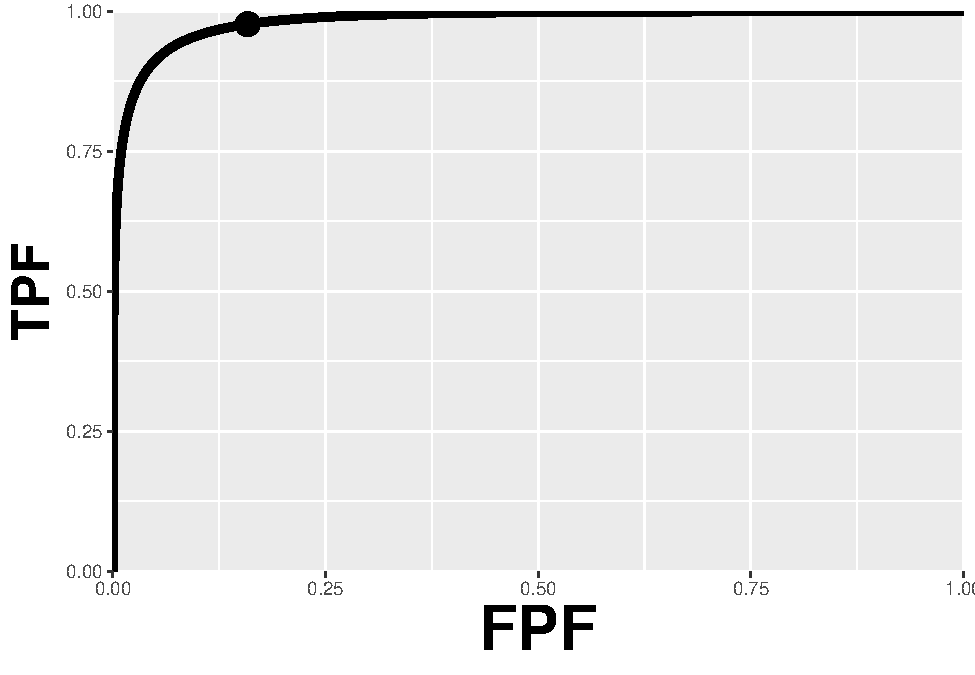
\includegraphics{03-modeling-binary-task_files/figure-latex/binaryTask-MainAnalyticalROC-1.pdf}
\caption{\label{fig:binaryTask-MainAnalyticalROC}ROC curve predicted by equal variance binormal model for mu = 3. The circled operating point corresponds to zeta = 1. The operating point falls exactly on the curve, as these are analytical results. Due to sampling variability, with finite numbers of cases, this is not observed in practice.}
\end{figure}

\hypertarget{physical-interpretation-of-the-mu-parameter}{%
\subsection{Physical interpretation of the mu-parameter}\label{physical-interpretation-of-the-mu-parameter}}

As a historical note, \(\mu\) is equivalent \citep{RN1318} to a signal detection theory variable denoted \(d'\) in the literature (pronounced ``dee-prime''). It can be thought of as the \emph{perceptual signal to noise ratio} (pSNR) of diseased cases relative to non-diseased ones. It is a measure of reader expertise and / or ease of detectability of the disease. SNR is a term widely used in engineering, specifically in signal detection theory \citep{RN298, RN346}, it dates to the early 1940s when one had the problem \citep{USAirForce1947} of detecting faint radar reflections from a plane against a background of noise. The reader may be aware of the ``rule-of-thumb'' that if SNR exceeds three the target is likely to be detected. It will be shown later that the area under the ROC curve is the probability that a diseased case Z-sample is greater than that of a non-diseased one. The following code snippet shows that for \(\mu = 3\), the probability of detection is 98.3 percent.

\begin{Shaded}
\begin{Highlighting}[]
\KeywordTok{pnorm}\NormalTok{(}\DecValTok{3}\OperatorTok{/}\KeywordTok{sqrt}\NormalTok{(}\DecValTok{2}\NormalTok{))}
\CommentTok{\#\textgreater{} [1] 0.983}
\end{Highlighting}
\end{Shaded}

For electrical signals, SNR can be measured with instruments but, in the context of decisions, measured is the perceptual SNR. Physical characteristics that differentiate non-diseased from diseased cases, and how well they are displayed will affect it; in addition the eye-sight of the observer is an obvious factor; not so obvious is how information is processed by the cognitive system, and the role of the observer's experience in making similar decisions (i.e., expertise).

\hypertarget{assigning-confidence-intervals-to-an-operating-point}{%
\section{Assigning confidence intervals to an operating point}\label{assigning-confidence-intervals-to-an-operating-point}}

\begin{itemize}
\tightlist
\item
  The notation in the following equations follows that introduced in Chapter 02.
\item
  A \((1-\alpha)\) confidence interval (CI) of a statistic is the range that is expected to contain the true value of the statistic with probability \((1-\alpha)\).
\item
  It should be clear that a 99 percent CI is wider than a 95 percent CI, and a 90percentCI is narrower; in general, the higher the confidence that the interval contains the true value, the wider the range of the CI.
\item
  Calculation of a parametric confidence interval requires a distributional assumption (non-parametric estimation methods, which use resampling methods, are described later). With a distributional assumption, the method being described now, the parameters of the distribution can be estimated, and since the distribution accounts for variability, the needed confidence interval estimate follows.
\item
  With TPF and FPF, each of which involves a ratio of two integers, it is convenient to assume a \emph{binomial} distribution for the following reason:
\item
  The diagnosis ``non-diseased'' vs.~``diseased'' is a Bernoulli trial, i.e., one whose outcome is binary.
\item
  A Bernoulli trial is like a coin-toss, a special coin whose probability of landing ``diseased'' face up is \(p\), which is not necessarily 0.5 as with a real coin.
\item
  It is a theorem in statistics that the total number of Bernoulli outcomes of one type, e.g., \(n(FP)\), is a binomial-distributed random variable, with success probability \(\widehat{FPF}\) and trial size \(K_1\). The circumflex denotes an estimate.
\end{itemize}

\begin{equation} 
n(FP) \sim B\left ( K_1, \widehat{FPF} \right )
\label{eq:binaryTask-BinDistrFPF}
\end{equation}

In Eqn. \eqref{eq:binaryTask-BinDistrFPF}, \(B(n,p)\) denotes the binomial distribution with success probability \(p\) and trial size \(n\):

\begin{equation} 
\left.\begin{matrix}
k \sim B\left ( n, p \right )\\
k=0,1,2,...,n\\
\end{matrix}\right\}
\label{eq:binaryTask-BinDistrDef}
\end{equation}

Eqn. \eqref{eq:binaryTask-BinDistrDef} states that \(k\) is a random sample from the binomial distribution \(B(n,p)\). For reference, the probability mass function \(\text{pmf}\) of \(B(n,p)\) is defined by (the subscript \(Bin\) denotes a binomial distribution):

\begin{equation} 
\text{pmf}_{Bin}\left ( k;n,p \right )=\binom{n}{k}p^k(1-p)^{n-k}
\label{eq:binaryTask-BinDistrDef2}
\end{equation}

For a discrete distribution, one has probability \emph{mass} function; in contrast, for a continuous distribution one has a probability \emph{density} function.

The binomial coefficient \(\binom{n}{k}\) appearing in Eqn. \eqref{eq:binaryTask-BinDistrDef2}, to be read as ``\(n\) pick \(k\)'', is defined by:

\begin{equation} 
\binom{n}{k}=\frac{n!}{k!(n-k)!}
\label{eq:binaryTask-BinCoeff}
\end{equation}

From the properties of the binomial distribution the variance of n(FP) is given by:

\begin{equation} 
\sigma_{n(FP)}^2=K_1\widehat{FPF}\left ( 1 - \widehat{FPF} \right )
\label{eq:binaryTask-Var-n-FP}
\end{equation}

It follows that \(FPF\) has mean \(\widehat{FPF}\) and variance \(\sigma_{FPF}^2\) given by (using theorem \(Var(aX) = a^2 Var(X)\), where \(a\) is a constant, equal to \(1/K_1\) in this case):

\begin{equation} 
\sigma_{FPF}^2 = \frac{\widehat{FPF}\left ( 1 - \widehat{FPF} \right )}{K_1}
\label{eq:binaryTask-Var-FPF}
\end{equation}

For large \(K_1\) the distribution of \(FPF\) approaches a normal distribution as follows:

\[FPF \sim N\left ( \widehat{FPF}, \sigma_{FPF}^2 \right )\]

This immediately allows us to write down the confidence interval for \(\widehat{FPF}\), i.e., \(\pm z_{\alpha/2}\) around \(\widehat{FPF}\).

\begin{equation} 
CI_{1-\alpha}^{FPF}=\left ( \widehat{FPF} - z_{\alpha/2} \sigma_{FPF}, \widehat{FPF} + z_{\alpha/2} \sigma_{FPF} \right )
\label{eq:binaryTask-CI-FPF}
\end{equation}

In Eqn. \eqref{eq:binaryTask-CI-FPF}, \(z_{\alpha/2}\) is the upper \(\alpha/2\) quantile of the unit normal distribution, i.e., the area to the \emph{right} under the unit normal distribution pdf from \(z_{\alpha/2}\) to \(\infty\) equals \(\alpha/2\). It is the complement (i.e., plus goes to minus) of \(\Phi^{-1}(\alpha/2)\) introduced earlier; the difference is that the latter uses the area to the \emph{left}. The following code might help.

\begin{Shaded}
\begin{Highlighting}[]
\NormalTok{alpha \textless{}{-}}\StringTok{ }\FloatTok{0.05}
\CommentTok{\# this is z\_\{\textbackslash{}alpha/2\}, the upper \textbackslash{}alpha/2 quantile}
\KeywordTok{qnorm}\NormalTok{(}\DecValTok{1}\OperatorTok{{-}}\NormalTok{alpha}\OperatorTok{/}\DecValTok{2}\NormalTok{) }
\CommentTok{\#\textgreater{} [1] 1.96}
\CommentTok{\# this is \textbackslash{}Phi\^{}\{{-}1\}(\textbackslash{}alpha/2), the lower \textbackslash{}alpha/2 quantile}
\KeywordTok{qnorm}\NormalTok{(alpha}\OperatorTok{/}\DecValTok{2}\NormalTok{)   }
\CommentTok{\#\textgreater{} [1] {-}1.96}
\end{Highlighting}
\end{Shaded}

Here is the definition of \(z_{\alpha/2}\):

\begin{equation} 
\left.
\begin{aligned} 
z_{\alpha/2} &=\Phi^{-1}\left ( 1-\alpha/2 \right )\\
\alpha/2&=\int_{z_{\alpha/2}}^{\infty}\phi(z)dz\\ 
&= 1-\Phi(z_{\alpha/2})\\
\\
\end{aligned}
\right \} 
\label{eq:binaryTask-def-z-alpha2}
\end{equation}

The normal approximation is adequate if both of the following two conditions are both met: \(K_1\widehat{FPF} > 10\) and \(K_1(1-\widehat{FPF}) > 10\). This means, essentially, that \(\widehat{FPF}\) is not too close to zero or 1.

Similarly, an approximate symmetric \((1-\alpha)\) confidence interval for TPF is:

\begin{equation} 
CI_{1-\alpha}^{TPF}=\left ( \widehat{TPF} - z_{\alpha/2} \sigma_{TPF}, \widehat{TPF} + z_{\alpha/2} \sigma_{TPF} \right )
\label{eq:binaryTask-CI-TPF}
\end{equation}

In Eqn. \eqref{eq:binaryTask-CI-TPF},

\begin{equation} 
\sigma_{TPF}^2 = \frac{\widehat{TPF}\left ( 1 - \widehat{TPF} \right )}{K_2}
\label{eq:binaryTask-Var-TPF}
\end{equation}

The confidence intervals are largest when the probabilities (FPF or TPF) are close to 0.5 and decrease inversely as the square root of the relevant number of cases. The symmetric binomial distribution based estimates can stray outside the allowed range (0 to 1). Exact confidence intervals9 that are asymmetric around the central value and which are guaranteed to be in the allowed range can be calculated: it is implemented in \texttt{R} in function \texttt{binom.test()}and used below (The approximate confidence intervals can exceed the allowed ranges, but the exact confidence intervals do not):

\begin{Shaded}
\begin{Highlighting}[]
\KeywordTok{options}\NormalTok{(}\DataTypeTok{digits=}\DecValTok{3}\NormalTok{)}
\NormalTok{seed \textless{}{-}}\StringTok{ }\DecValTok{100}\NormalTok{;}\KeywordTok{set.seed}\NormalTok{(seed)}
\NormalTok{alpha \textless{}{-}}\StringTok{ }\FloatTok{0.05}\NormalTok{;K1 \textless{}{-}}\StringTok{ }\DecValTok{99}\NormalTok{;K2 \textless{}{-}}\StringTok{ }\DecValTok{111}\NormalTok{;mu \textless{}{-}}\StringTok{ }\DecValTok{5}\NormalTok{;zeta \textless{}{-}}\StringTok{ }\NormalTok{mu}\OperatorTok{/}\DecValTok{2}
\KeywordTok{cat}\NormalTok{(}\StringTok{"alpha = "}\NormalTok{, alpha, }
    \StringTok{"}\CharTok{\textbackslash{}n}\StringTok{K1 = "}\NormalTok{, K1, }
    \StringTok{"}\CharTok{\textbackslash{}n}\StringTok{K2 = "}\NormalTok{, K2, }
    \StringTok{"}\CharTok{\textbackslash{}n}\StringTok{mu = "}\NormalTok{, mu, }
    \StringTok{"}\CharTok{\textbackslash{}n}\StringTok{zeta = "}\NormalTok{, zeta, }\StringTok{"}\CharTok{\textbackslash{}n}\StringTok{"}\NormalTok{)}
\CommentTok{\#\textgreater{} alpha =  0.05 }
\CommentTok{\#\textgreater{} K1 =  99 }
\CommentTok{\#\textgreater{} K2 =  111 }
\CommentTok{\#\textgreater{} mu =  5 }
\CommentTok{\#\textgreater{} zeta =  2.5}
\NormalTok{z1 \textless{}{-}}\StringTok{ }\KeywordTok{rnorm}\NormalTok{(K1)}
\NormalTok{z2 \textless{}{-}}\StringTok{ }\KeywordTok{rnorm}\NormalTok{(K2) }\OperatorTok{+}\StringTok{ }\NormalTok{mu}
\NormalTok{nTN \textless{}{-}}\StringTok{ }\KeywordTok{length}\NormalTok{(z1[z1 }\OperatorTok{\textless{}}\StringTok{ }\NormalTok{zeta])}
\NormalTok{nTP \textless{}{-}}\StringTok{ }\KeywordTok{length}\NormalTok{(z2[z2 }\OperatorTok{\textgreater{}=}\StringTok{ }\NormalTok{zeta])}
\NormalTok{Sp \textless{}{-}}\StringTok{ }\NormalTok{nTN}\OperatorTok{/}\NormalTok{K1;Se \textless{}{-}}\StringTok{ }\NormalTok{nTP}\OperatorTok{/}\NormalTok{K2}
\KeywordTok{cat}\NormalTok{(}\StringTok{"Specificity = "}\NormalTok{, Sp, }
    \StringTok{"}\CharTok{\textbackslash{}n}\StringTok{Sensitivity = "}\NormalTok{, Se, }\StringTok{"}\CharTok{\textbackslash{}n}\StringTok{"}\NormalTok{)}
\CommentTok{\#\textgreater{} Specificity =  0.99 }
\CommentTok{\#\textgreater{} Sensitivity =  0.991}

\CommentTok{\# Approx binomial tests}
\KeywordTok{cat}\NormalTok{(}\StringTok{"approx 95percent CI on Specificity = "}\NormalTok{, }
    \OperatorTok{{-}}\KeywordTok{abs}\NormalTok{(}\KeywordTok{qnorm}\NormalTok{(alpha}\OperatorTok{/}\DecValTok{2}\NormalTok{))}\OperatorTok{*}\KeywordTok{sqrt}\NormalTok{(Sp}\OperatorTok{*}\NormalTok{(}\DecValTok{1}\OperatorTok{{-}}\NormalTok{Sp)}\OperatorTok{/}\NormalTok{K1)}\OperatorTok{+}\NormalTok{Sp, }
    \OperatorTok{+}\KeywordTok{abs}\NormalTok{(}\KeywordTok{qnorm}\NormalTok{(alpha}\OperatorTok{/}\DecValTok{2}\NormalTok{))}\OperatorTok{*}\KeywordTok{sqrt}\NormalTok{(Sp}\OperatorTok{*}\NormalTok{(}\DecValTok{1}\OperatorTok{{-}}\NormalTok{Sp)}\OperatorTok{/}\NormalTok{K1)}\OperatorTok{+}\NormalTok{Sp,}\StringTok{"}\CharTok{\textbackslash{}n}\StringTok{"}\NormalTok{)}
\CommentTok{\#\textgreater{} approx 95percent CI on Specificity =  0.97 1.01}

\CommentTok{\# Exact binomial test}
\NormalTok{ret \textless{}{-}}\StringTok{ }\KeywordTok{binom.test}\NormalTok{(nTN, K1, }\DataTypeTok{p =}\NormalTok{ nTN}\OperatorTok{/}\NormalTok{K1)}
\KeywordTok{cat}\NormalTok{(}\StringTok{"Exact 95percent CI on Specificity = "}\NormalTok{, }
    \KeywordTok{as.numeric}\NormalTok{(ret}\OperatorTok{$}\NormalTok{conf.int),}\StringTok{"}\CharTok{\textbackslash{}n}\StringTok{"}\NormalTok{)}
\CommentTok{\#\textgreater{} Exact 95percent CI on Specificity =  0.945 1}

\CommentTok{\# Approx binomial tests}
\KeywordTok{cat}\NormalTok{(}\StringTok{"approx 95percent CI on Sensitivity = "}\NormalTok{, }
    \OperatorTok{{-}}\KeywordTok{abs}\NormalTok{(}\KeywordTok{qnorm}\NormalTok{(alpha}\OperatorTok{/}\DecValTok{2}\NormalTok{))}\OperatorTok{*}\KeywordTok{sqrt}\NormalTok{(Se}\OperatorTok{*}\NormalTok{(}\DecValTok{1}\OperatorTok{{-}}\NormalTok{Se)}\OperatorTok{/}\NormalTok{K2)}\OperatorTok{+}\NormalTok{Se, }
    \OperatorTok{+}\KeywordTok{abs}\NormalTok{(}\KeywordTok{qnorm}\NormalTok{(alpha}\OperatorTok{/}\DecValTok{2}\NormalTok{))}\OperatorTok{*}\KeywordTok{sqrt}\NormalTok{(Se}\OperatorTok{*}\NormalTok{(}\DecValTok{1}\OperatorTok{{-}}\NormalTok{Se)}\OperatorTok{/}\NormalTok{K2)}\OperatorTok{+}\NormalTok{Se,}\StringTok{"}\CharTok{\textbackslash{}n}\StringTok{"}\NormalTok{)}
\CommentTok{\#\textgreater{} approx 95percent CI on Sensitivity =  0.973 1.01}

\CommentTok{\# Exact binomial test}
\NormalTok{ret \textless{}{-}}\StringTok{ }\KeywordTok{binom.test}\NormalTok{(nTP, K2, }\DataTypeTok{p =}\NormalTok{ nTP}\OperatorTok{/}\NormalTok{K2)}
\KeywordTok{cat}\NormalTok{(}\StringTok{"Exact 95percent CI on Sensitivity = "}\NormalTok{, }
    \KeywordTok{as.numeric}\NormalTok{(ret}\OperatorTok{$}\NormalTok{conf.int),}\StringTok{"}\CharTok{\textbackslash{}n}\StringTok{"}\NormalTok{)}
\CommentTok{\#\textgreater{} Exact 95percent CI on Sensitivity =  0.951 1}
\end{Highlighting}
\end{Shaded}

Note the usage of the \emph{absolute} value of the \texttt{qnorm()} function; \texttt{qnorm} is the lower quantile function for the unit normal distribution, identical to \(\Phi^{-1}(0.025)\), i.e., about -1.96, and \(z_{\alpha/2}\) is the upper quantile.

\hypertarget{variability-in-sensitivity-and-specificity-the-beam-et-al-study}{%
\section{Variability in sensitivity and specificity: the Beam et al study}\label{variability-in-sensitivity-and-specificity-the-beam-et-al-study}}

In this study \citep{RN1087} fifty accredited mammography centers were randomly sampled in the United States. ``Accredited'' is a legal/regulatory term implying, among other things, that the radiologists interpreting the breast cases were ``board certified'' by the American Board of Radiology. One hundred eight (108) certified radiologists from these centers gave blinded interpretation to a common set of 79 randomly selected enriched screening cases containing 45 cases with cancer and the rest normal or with benign lesions. Ground truth for these women had been established either by biopsy or by 2-year follow-up (establishing truth is often the most time consuming part of conducting an ROC study). The observed range of sensitivity (TPF) was 53percent and the range of FPF was 63percent; the corresponding range for AUC was 21percent, Table \ref{tab:binaryTask0BeamStudy}.

\begin{Shaded}
\begin{Highlighting}[]
\NormalTok{results \textless{}{-}}\StringTok{ }\KeywordTok{array}\NormalTok{(}\DataTypeTok{dim =} \KeywordTok{c}\NormalTok{(}\DecValTok{3}\NormalTok{,}\DecValTok{3}\NormalTok{))}
\NormalTok{results[}\DecValTok{1}\NormalTok{,] \textless{}{-}}\StringTok{ }\KeywordTok{c}\NormalTok{(}\FloatTok{46.7}\NormalTok{, }\DecValTok{100}\NormalTok{, }\FloatTok{53.3}\NormalTok{)}
\NormalTok{results[}\DecValTok{2}\NormalTok{,] \textless{}{-}}\StringTok{ }\KeywordTok{c}\NormalTok{(}\FloatTok{36.3}\NormalTok{, }\FloatTok{99.3}\NormalTok{, }\FloatTok{63.0}\NormalTok{)}
\NormalTok{results[}\DecValTok{3}\NormalTok{,] \textless{}{-}}\StringTok{ }\KeywordTok{c}\NormalTok{(}\FloatTok{0.74}\NormalTok{, }\FloatTok{0.95}\NormalTok{, }\FloatTok{0.21}\NormalTok{)}
\NormalTok{df \textless{}{-}}\StringTok{ }\KeywordTok{as.data.frame}\NormalTok{(results)}
\KeywordTok{rownames}\NormalTok{(df) \textless{}{-}}\StringTok{ }\KeywordTok{c}\NormalTok{(}\StringTok{"Sensiivity"}\NormalTok{,}\StringTok{"Specificity"}\NormalTok{,}\StringTok{"AUC"}\NormalTok{)}
\KeywordTok{colnames}\NormalTok{(df) \textless{}{-}}\StringTok{ }\KeywordTok{c}\NormalTok{(}\StringTok{"Min"}\NormalTok{,}\StringTok{"Max"}\NormalTok{,}\StringTok{"Range"}\NormalTok{)}
\end{Highlighting}
\end{Shaded}

\begin{table}

\caption{\label{tab:binaryTask0BeamStudy}The variability of 108 radiologists on a common dataset of screening mammograms. Note the reduced variability when one uses AUC, which accounts for variations in reporting thresholds (AUC variability range is 21percent compared to 53percent for sensitivity and 63percent for specificity).}
\centering
\begin{tabular}[t]{l|r|r|r}
\hline
  & Min & Max & Range\\
\hline
Sensiivity & 46.70 & 100.00 & 53.30\\
\hline
Specificity & 36.30 & 99.30 & 63.00\\
\hline
AUC & 0.74 & 0.95 & 0.21\\
\hline
\end{tabular}
\end{table}

\begin{figure}
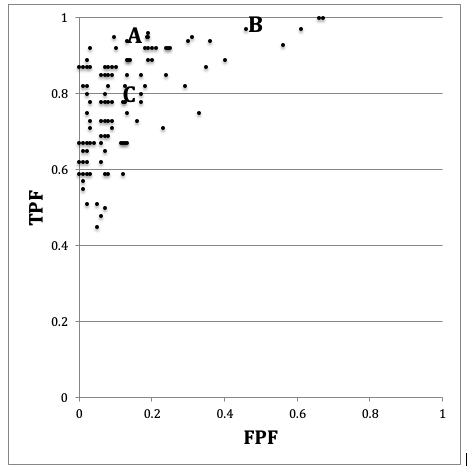
\includegraphics[width=0.8\linewidth]{images/BeamStudy} \caption{Schematic, patterned from the Beam et al study, showing the ROC operating points of 108 mammographers. Wide variability in sensitivity (40percent) and specificity (45percent) are evident. Radiologists (B) and (C) appear to be trading sensitivity for specificity and vice versa, while radiologist A's performance is intrinsically superior. See summary of important principles below.}\label{fig:BeamStudyFig}
\end{figure}

In Fig. \ref{fig:BeamStudyFig}, a schematic of the data, if one looks at the points labeled (B) and (C) one can mentally construct a smooth ROC curve that starts at (0,0), passes roughly through these points and ends at (1,1). In this sense, the intrinsic performances (i.e., AUCs or equivalently the parameter) of the two radiologists are similar. The only difference between them is that radiologist (B) is using lower threshold relative to the radiologist (C). Radiologist (C) is more concerned with minimizing FPs while radiologist (B) is more concerned with maximizing sensitivity. By appropriate feedback radiologist (C) can perhaps be induced to change the threshold to that of radiologist (B), or they both could be induced to achieve a happy compromise. An example of feedback might be: ``you are missing too many cancers and this could get us all into trouble; worry less about reduced specificity and more about increasing your sensitivity''. In contrast, radiologist (A) has intrinsically greater performance (B) or (C). No change in threshold is going to get the other two to a similar level of performance as radiologist A. Extensive training will be needed to bring the under-performing radiologists to the expert level represented by radiologist A.

Fig. \ref{fig:BeamStudyFig} and Table \ref{tab:binaryTask0BeamStudy} illustrate several important principles.
1. Since an operating point is characterized by two values, unless both numbers are higher (e.g., radiologist A vs.~B or C), it is difficult to unambiguously compare them.
2. While sensitivity and specificity depend on the reporting threshold, the area under the ROC plot is independent of it. Using the area under the ROC curve one can unambiguously compare two readers.
3. Combining sensitivity and the complement of specificity into a single AUC measure yields the additional benefit of lower variability. In Fig. \ref{fig:BeamStudyFig}, the range for sensitivity is 53 percent while that for specificity is 63 percent. In contrast, the range for AUC is only 21 percent. This means that much of the observed variations in sensitivity and specificity are due to variations in thresholds, and using AUC eliminates this source of variability. Decreased variability of a measure is a highly desirable characteristic as it implies the measurement is more precise, making it easier to detect genuine changes between readers and / or modalities.

\hypertarget{binaryTask-Summary}{%
\section{Summary}\label{binaryTask-Summary}}

\hypertarget{binaryTask-Discussion}{%
\section{Discussion}\label{binaryTask-Discussion}}

The concepts of sensitivity and specificity are of fundamental importance and are widely used in the medical imaging literature. However, it is important to realize that sensitivity and specificity do not provide a complete picture of diagnostic performance, since they represent performance at a particular threshold. As demonstrated in Fig. 3.6, expert observers can and do operate at different points, and the reporting threshold depends on cost-benefit considerations, disease prevalence and personal reporting styles. If using sensitivity and specificity the dependence on reporting threshold often makes it difficult to unambiguously compare observers. Even if one does compare them, there is loss of statistical power (equivalent to loss of precision of the measurement) due to the additional source of variability introduced by the varying thresholds.

The ROC curve is the locus of operating points as the threshold is varied. It and AUC are completely defined by the parameter of the equal variance binormal model. Since both are independent of reporting threshold , they overcome the ambiguity inherent in comparing sensitivity/specificity pairs. Both are scalar measures of performance. AUC is widely used in assessing imaging systems. It should impress the reader that a subjective internal sensory perception of disease presence and an equally subjective internal threshold can be translated into an objective performance measure, such as the area under an ROC curve or equivalently, the parameter. The latter has the physical meaning of a perceptual signal to noise ratio.

The ROC curve predicted by the equal variance binormal model has a useful property, namely, as the threshold is lowered, its slope decreases monotonically. The predicted curve never crosses the chance diagonal, i.e., the predicted ROC curve is ``proper''. Unfortunately, as one will see later, most ROC datasets are inconsistent with this model: rather, they are more consistent with a model where the diseased distribution has variance greater than unity. The consequence of this is an ``improper'' ROC curve, where in a certain range, which may be difficult to see when the data is plotted on a linear scale, the predicted curve actually crosses the chance diagonal and then its slope increases as it hooks up to reach (1,1). The predicted worse than chance performance is unreasonable. Models of ROC curves have been developed that do not have this unreasonable behavior: Chapter 17, Chapter 18 and Chapter 20.

The properties of the unit normal distribution and the binomial distribution were used to derive parametric confidence intervals for sensitivity and specificity. These were compared to exact confidence intervals. An important study was reviewed showing wide variability in sensitivity and specificity for radiologists interpreting a common set of cases in screening mammography, but smaller variability in areas under the ROC curve. This is because much of the variability in sensitivity and specificity is due to variation of the reporting threshold, which does not affect the area under the ROC curve. This is an important reason for preferring comparisons based on area under the ROC curve to those based on comparing sensitivity/specificity pairs.

This chapter has been demonstrated the equal variance binormal model with R examples. These were used to illustrate important concepts of case-sampling variability and its dependence on the numbers of cases. Again, while relegated for organizational reasons to online appendices, these appendices are essential components of the book. Most of the techniques demonstrated there will be reused in the remaining chapters. The motivated reader can learn much from studying the online material and running the different main-level functions contained in the software-directory corresponding to this chapter.

\hypertarget{binaryTask-references}{%
\section{References}\label{binaryTask-references}}

\hypertarget{ratingsParadigm}{%
\chapter{Ratings Paradigm}\label{ratingsParadigm}}

\hypertarget{introduction}{%
\section{Introduction}\label{introduction}}

In Chapter \ref{binaryTask0} the binary paradigm and associated concepts (e.g., sensitivity, specificity) were introduced. Chapter \ref{binaryTask} introduced the concepts of a random scalar decision variable, or z-sample for each case, which is compared, by the observer to a fixed reporting threshold \(\zeta\), resulting in two types of decisions. It described a statistical model, characterized by two unit-variance normal distributions separated by \(\mu\), for the binary task. The concept of an underlying receiver operating characteristic (ROC) curve with the reporting threshold defining an operating point on the curve was introduced and the advisability of using the area under the curve as a measure of performance, which is independent of reporting threshold, was stressed.

In this chapter the more commonly used ratings method will be described, which yields greater definition to the underlying ROC curve than just one operating point obtained in the binary task, and moreover, is more efficient. In this method, the observer assigns a rating to each case. Described first is a typical ROC counts table and how operating points (i.e., pairs of FPF and TPF values) are calculated from the counts data. A labeling convention for the operating points is introduced. Notation is introduced for the observed integers in the counts table and the rules for calculating operating points are expressed as formulae and implemented in R. The ratings method is contrasted to the binary method, in terms of efficiency and practicality. A theme occurring repeatedly in this book, that the ratings are not numerical values but rather they are ordered labels is illustrated with an example. A method of collecting ROC data on a 6-point scale is described that has the advantage of yielding an unambiguous single operating point. The forced choice paradigm is described. Two controversies are described: one on the utility of discrete (e.g., 1 to 6) vs.~quasi-continuous (e.g., 0 to 100) ratings and the other on the applicability of a clinical screening mammography-reporting scale for ROC analyses. Both of these are important issues and it would be a disservice to the readers of the book if the author did not express his position on them.

\hypertarget{the-roc-counts-table}{%
\section{The ROC counts table}\label{the-roc-counts-table}}

In a positive-directed rating scale with five discrete levels, the ratings could be the ordered labels:

\begin{itemize}
\tightlist
\item
  ``1'': definitely non-diseased,
\item
  ``2'': probably non-diseased,
\item
  ``3'': could be non-diseased or diseased,
\item
  ``4'': probably diseased,
\item
  ``5'': definitely diseased.
\end{itemize}

At the conclusion of the ROC study an ROC counts table is constructed. This is the generalization to rating studies of the 2 x 2 decision vs.~truth table introduced in (book) Chapter 02, Table 2.1. This type of data representation is sometimes called a frequency table, but frequency usually means a rate of number of events per some unit, so the author prefers the clearer term ``counts''.

Table \ref{tab:ratingsParadigmTable1} is a representative counts table for a 5-rating study that summarizes the collected data. It is the starting point for analysis. It lists the number of counts in each ratings bin, listed separately for non-diseased and diseased cases, respectively. The data is from an actual clinical study \citep{RN4343}.

\begin{table}

\caption{\label{tab:ratingsParadigmTable1}Representative counts table.}
\centering
\begin{tabular}[t]{l|r|r|r|r|r}
\hline
  & $r = 5$ & $r = 4$ & $r = 3$ & $r = 2$ & $r = 1$\\
\hline
non-diseased & 1 & 2 & 8 & 19 & 30\\
\hline
diseased & 22 & 12 & 5 & 6 & 5\\
\hline
\end{tabular}
\end{table}

In this table:

\begin{itemize}
\tightlist
\item
  \(r = 5\) means ``rating equal to 5''
\item
  \(r = 4\) means ``rating equal to 4''
\item
  Etc.
\end{itemize}

There are \(K_1 = 60\) non-diseased cases and \(K_2 = 50\) diseased cases. Of the 60 non-diseased cases, one received the ``5'' rating, two the ``4'' rating, eight the ``3'' rating, 19 the ``2'' rating and 30 were assigned the ``1'' rating. The distribution of counts is tilted towards the ``1'' rating end, but there is some spread and one actually non-diseased case appeared definitely diseased to the observer. In contrast, the distribution of the diseased cases is tilted towards the ``5'' rating end. Of the 50 diseased cases, 22 received the ``5'' rating, 12 the ``4'' rating, five the ``3'' rating, six the ``2'' rating and five the ``1'' rating. A little thought should convince you that the observed tilting of the counts, towards the ``1'' end for actually non-diseased cases, and towards the ``5'' end for actually diseased cases, is reasonable.

The spread appears to be more pronounced for the diseased cases, e.g., five of the 50 cases appeared to be definitely non-diseased to the observer. However, one should be forewarned not to jump to conclusions about the spread of the data being larger for diseased than for non-diseased cases. While it turns out to be true as will be shown later, the \textbf{ratings are merely ordered labels}, and modeling is required, to be described in Chapter \ref{BinMod}, that uses only the \emph{ordering information} implicit in the labels, not the \emph{actual values}, to reach quantitative conclusions.

\hypertarget{operating-points-from-counts-table}{%
\section{Operating points from counts table}\label{operating-points-from-counts-table}}

Table \ref{tab:ratingsParadigmTable2} illustrates how ROC operating points are calculated from the cell counts. In this table:

\begin{itemize}
\tightlist
\item
  \(r\geq 5\) means ``counting ratings greater than or equal to 5''
\item
  \(r\geq 4\) means ``counting ratings greater than or equal to 4''
\item
  Etc.
\end{itemize}

\begin{table}

\caption{\label{tab:ratingsParadigmTable2}Computation of operating points from cell counts.}
\centering
\begin{tabular}[t]{l|r|r|r|r|r}
\hline
  & $r\geq 5$ & $r\geq 4$ & $r\geq 3$ & $r\geq 2$ & $r\geq 1$\\
\hline
FPF & 0.0167 & 0.05 & 0.1833 & 0.5 & 1\\
\hline
TPF & 0.4400 & 0.68 & 0.7800 & 0.9 & 1\\
\hline
\end{tabular}
\end{table}

One starts with non-diseased cases that were rated five or more (in this example, since 5 is the highest allowed rating, the ``or more'' clause is inconsequential) and divides by the total number of non-diseased cases, \(K_1 = 60\). This yields the abscissa of the lowest non-trivial operating point, namely \(FPF_{\ge5}\) = 1/60 = 0.017. The subscript on FPF is intended to make explicit which ratings are being cumulated. The corresponding ordinate is obtained by dividing the number of diseased cases rated ``5'' or more and dividing by the total number of diseased cases, \(K_2 = 50\), yielding \(TPF_{\ge5}\) = 22/50 = 0.440. Therefore, the coordinates of the lowest operating point are (0.017, 0.44). The abscissa of the next higher operating point is obtained by dividing the number of non-diseased cases that were rated ``4'' or more and dividing by the total number of non-diseased cases, i.e., \(TPF_{\ge4}\) = 3/60 = 0.05. Similarly the ordinate of this operating point is obtained by dividing the number of diseased cases that were rated ``4'' or more and dividing by the total number of diseased cases, i.e., \(FPF_{\ge4}\) = 34/50 = 0.680. The procedure, which at each stage cumulates the number of cases equal to or greater (in the sense of increased confidence level for disease presence) than a specified ordered label, is repeated to yield the rest of the operating points listed in Table \ref{tab:ratingsParadigmTable2}. Since they are computed directly from the data, without any assumption, they are called empirical or observed operating points.

After doing this once, it would be nice to have a formula implementing the process, one use of which would be to code the procedure. But first one needs appropriate notation for the bin counts.

Let \(K_{1r}\) denote the number of non-diseased cases rated \(r\), and \(K_{2r}\) denote the number of diseased cases rated \(r\). For convenience, define dummy counts \(K_{1{(R+1)}}\) = \(K_{2{(R+1)}}\) = 0, where R is the number of ROC bins, \(R = 5\) in the current example. This construct allows inclusion of the origin (0,0) in the formulae. The range of \(r\) is \(r = 1,2,...,(R+1)\). Within each truth-state, the individual bin counts sum to the total number of non-diseased and diseased cases, respectively. The following equations summarize all this:

\begin{equation*} 
K_1=\sum_{r=1}^{R+1}K_{1r}
\end{equation*}

\begin{equation*} 
K_2=\sum_{r=1}^{R+1}K_{2r}
\end{equation*}

\begin{equation*} 
K_{1{(R+1)}} = K_{2{(R+1)}} = 0
\end{equation*}

\begin{equation*} 
r = 1,2,...,(R+1)
\end{equation*}

The operating points are defined by:

\begin{equation}
\left. 
\begin{aligned}
FPF_r=& \frac {1} {K_1} \sum_{s=r}^{R+1}K_{1s}\\
TPF_r=& \frac {1} {K_2} \sum_{s=r}^{R+1}K_{2s}
 \end{aligned}
\right \}
\label{eq:ratingsParadigm-FPF-TPF-from-counts}
\end{equation}

\hypertarget{numbering-the-points}{%
\subsection{Numbering the points}\label{numbering-the-points}}

The numbering \(n\) of the points follows the following convention: From Eqn. \eqref{eq:ratingsParadigm-FPF-TPF-from-counts}, the point corresponding to \(r=1\) would correspond to the upper right corner (1,1) of the ROC plot, a trivial operating point since it is common to all datasets, and is therefore not shown. The numbering starts with the next lower-left point, numbered \(n=1\), which corresponds to \(r=2\), the next lower-left point is numbered \(n=2\), corresponding to \(r=3\), etc., and the point numbered \(n=R-1=4\) is the lowest non-trivial operating point corresponding to \(r=R\) and finally \(r=R+1\) is the origin (0,0) of the ROC plot, which is also a trivial operating point, because it is common to all datasets, and is therefore not shown. \textbf{To summarize, the operating points are numbered starting with the upper right corner, numbered 1, and working down the curve, each time increasing the number by one. The total number of points is \(R-1\).} The relation between \(n\) and \(r\) in the formulae is:

\[n=r-1\]
An example of the numbering is shown in the next chapter, Fig. \ref{fig:empirical-AUC-EmpiricalPlot}.

\hypertarget{examples}{%
\subsection{Examples}\label{examples}}

In the following examples \(R = 5\) is the number of ROC bins and \(K_{1(R+1)}\) = \(K_{2(R+1)}\) = 0. If \(r = 1\) one gets the uppermost ``trivial'' operating point (1,1):

\begin{equation*} 
FPF_1=\frac {1} {K_1} \sum_{s=1}^{R+1}K_{1s} = \frac{60}{60} = 1\\
TPF_1=\frac {1} {K_2} \sum_{s=1}^{R+1}K_{2s} = \frac{50}{50} = 1
\end{equation*}

The uppermost non-trivial operating point is obtained for \(r = 2\), when:

\begin{equation*} 
FPF_2=\frac {1} {K_1} \sum_{s=2}^{R+1}K_{1s} = \frac{30}{60} = 0.5\\
TPF_2=\frac {1} {K_2} \sum_{s=2}^{R+1}K_{2s} = \frac{45}{50} = 0.9
\end{equation*}

The next lower operating point is obtained for \(r = 3\):

\begin{equation*} 
FPF_3=\frac {1} {K_1} \sum_{s=3}^{R+1}K_{1s} = \frac{11}{60} = 0.183\\
TPF_3=\frac {1} {K_2} \sum_{s=3}^{R+1}K_{2s} = \frac{39}{50} = 0.780
\end{equation*}

The next lower operating point is obtained for \(r = 4\):

\begin{equation*} 
FPF_4=\frac {1} {K_1} \sum_{s=4}^{R+1}K_{1s} = \frac{3}{60} = 0.05\\
TPF_4=\frac {1} {K_2} \sum_{s=4}^{R+1}K_{2s} = \frac{34}{50} = 0.680
\end{equation*}

The lowest non-trivial operating point is obtained for \(r = 5\):

\begin{equation*} 
FPF_5=\frac {1} {K_1} \sum_{s=5}^{R+1}K_{1s} = \frac{1}{60} = 0.017\\
TPF_5=\frac {1} {K_2} \sum_{s=5}^{R+1}K_{2s} = \frac{22}{50} = 0.440
\end{equation*}

The next value \(r = 6\) yields the trivial operating point (0,0):

\begin{equation*} 
FPF_6=\frac {1} {K_1} \sum_{s=6}^{R+1}K_{1s} = \frac{0}{60} = 0\\
TPF_6=\frac {1} {K_2} \sum_{s=6}^{R+1}K_{2s} = \frac{0}{50} = 0
\end{equation*}

This exercise shows explicitly that an R-rating ROC study can yield, at most, \(R + 1\) distinct non-trivial operating points; i.e., those corresponding to \(r=2,3,...,R\).

The modifier ``at most'' is needed, because if both counts (i.e., non-diseased and diseased) for bin \(r'\) are zeroes, then that operating point merges with the one immediately below-left of it:

\begin{equation*} 
FPF_{r'}=\frac {1} {K_1} \sum_{s={r'}}^{R+1}K_{1s} = \frac {1} {K_1} \sum_{s={r'+1}}^{R+1}K_{1s} = FPF_{r'+1}\\
\\
TPF_{r'}=\frac {1} {K_2} \sum_{s={r'}}^{R+1}K_{2s} = \frac {1} {K_2} \sum_{s={r'+1}}^{R+1}K_{2s} = TPF_{r'+1}
\end{equation*}

Since bin \(r'\) is unpopulated, one can re-label the bins to exclude the unpopulated bin, and now the total number of bins is effectively \(R-1\).

Since one is cumulating counts, which cannot be negative, the highest non-trivial operating point resulting from cumulating the 2 through 5 ratings has to be to the upper-right of the next adjacent operating point resulting from cumulating the 3 through 5 ratings. This in turn has to be to the upper-right of the operating point resulting from cumulating the 4 through 5 ratings. This in turn has to be to the upper right of the operating point resulting from the 5 ratings. In other words, as one cumulates ratings bins, the operating point must move monotonically up and to the right, or more accurately, the point cannot move down or to the left. If a particular bin has zero counts for non-diseased cases, and non-zero counts for diseased cases, the operating point moves vertically up when this bin is cumulated; if it has zero counts for diseased cases, and non-zero counts for non-diseased cases, the operating point moves horizontally to the right when this bin is cumulated.

\hypertarget{automating-all-this}{%
\section{Automating all this}\label{automating-all-this}}

It is useful to replace the preceding detailed explanation with a simple algorithm, as in the following code (see first seven lines):

\begin{Shaded}
\begin{Highlighting}[]
\KeywordTok{options}\NormalTok{(}\DataTypeTok{digits =} \DecValTok{3}\NormalTok{)}
\NormalTok{FPF \textless{}{-}}\StringTok{ }\KeywordTok{array}\NormalTok{(}\DecValTok{0}\NormalTok{,}\DataTypeTok{dim =}\NormalTok{ R)}
\NormalTok{TPF \textless{}{-}}\StringTok{ }\KeywordTok{array}\NormalTok{(}\DecValTok{0}\NormalTok{,}\DataTypeTok{dim =}\NormalTok{ R)}
\ControlFlowTok{for}\NormalTok{ (r }\ControlFlowTok{in}\NormalTok{ (R}\OperatorTok{+}\DecValTok{1}\NormalTok{)}\OperatorTok{:}\DecValTok{2}\NormalTok{) \{}
\NormalTok{  FPF[(R}\OperatorTok{+}\DecValTok{2}\NormalTok{)}\OperatorTok{{-}}\NormalTok{r] \textless{}{-}}\StringTok{ }\KeywordTok{sum}\NormalTok{(Ktr[}\DecValTok{1}\NormalTok{, r}\OperatorTok{:}\NormalTok{(R}\OperatorTok{+}\DecValTok{1}\NormalTok{)])}\OperatorTok{/}\KeywordTok{sum}\NormalTok{(Ktr[}\DecValTok{1}\NormalTok{,])}
\NormalTok{  TPF[(R}\OperatorTok{+}\DecValTok{2}\NormalTok{)}\OperatorTok{{-}}\NormalTok{r] \textless{}{-}}\StringTok{ }\KeywordTok{sum}\NormalTok{(Ktr[}\DecValTok{2}\NormalTok{, r}\OperatorTok{:}\NormalTok{(R}\OperatorTok{+}\DecValTok{1}\NormalTok{)])}\OperatorTok{/}\KeywordTok{sum}\NormalTok{(Ktr[}\DecValTok{2}\NormalTok{,])    }
\NormalTok{\}}
\NormalTok{df \textless{}{-}}\StringTok{ }\KeywordTok{data.frame}\NormalTok{(}\DataTypeTok{FPF =}\NormalTok{ FPF, }\DataTypeTok{TPF =}\NormalTok{ TPF)}
\NormalTok{df \textless{}{-}}\StringTok{ }\KeywordTok{t}\NormalTok{(df)}
\KeywordTok{print}\NormalTok{(df)}
\CommentTok{\#\textgreater{}     [,1]  [,2] [,3]  [,4]}
\CommentTok{\#\textgreater{} FPF  0.5 0.817 0.95 0.983}
\CommentTok{\#\textgreater{} TPF  0.1 0.220 0.32 0.560}
\NormalTok{mu \textless{}{-}}\StringTok{ }\KeywordTok{qnorm}\NormalTok{(.}\DecValTok{5}\NormalTok{)}\OperatorTok{+}\KeywordTok{qnorm}\NormalTok{(.}\DecValTok{9}\NormalTok{);sigma \textless{}{-}}\StringTok{ }\DecValTok{1}
\NormalTok{Az \textless{}{-}}\StringTok{ }\KeywordTok{pnorm}\NormalTok{(mu}\OperatorTok{/}\KeywordTok{sqrt}\NormalTok{(}\DecValTok{2}\NormalTok{))}
\KeywordTok{cat}\NormalTok{(}\StringTok{"uppermost point based estimate of mu = "}\NormalTok{, mu, }\StringTok{"}\CharTok{\textbackslash{}n}\StringTok{"}\NormalTok{)}
\CommentTok{\#\textgreater{} uppermost point based estimate of mu =  1.28}
\KeywordTok{cat}\NormalTok{(}\StringTok{"corresponding estimate of Az = "}\NormalTok{, Az, }\StringTok{"}\CharTok{\textbackslash{}n}\StringTok{"}\NormalTok{)}
\CommentTok{\#\textgreater{} corresponding estimate of Az =  0.818}
\end{Highlighting}
\end{Shaded}

Notice that the values of the arrays \texttt{FPF} and \texttt{TPF} are identical to those listed in Table \ref{tab:ratingsParadigmTable2}. Regarding the last four lines of code, it was shown in Chapter \ref{binaryTask} that in the equal variance binormal model the operating point determines the parameters \(\mu\) = 1.282, Eqn. \eqref{eq:binaryTask-SolveForMu}, or equivalently \(A_{z;\sigma = 1}\) = 0.818, Eqn. \eqref{eq:binaryTask-Az-EqVarModel2}. The last four lines illustrate the application of these formulae using the coordinates (0.5, 0.9) of the uppermost non-trivial operating point, i.e., one is fitting the equal variance model to the uppermost operating point.

Shown next is the equal-variance model fit to the uppermost non-trivial operating point, left plot, and for comparison, the right plot is the unequal variance model fit to all operating points. The unequal variance model is the subject of an upcoming chapter.

\begin{Shaded}
\begin{Highlighting}[]
\CommentTok{\# equal variance fit to uppermost operating point}
\NormalTok{p1 \textless{}{-}}\StringTok{ }\KeywordTok{plotROC}\NormalTok{ (mu, sigma, FPF, TPF)}
\CommentTok{\# the following values are from unequal{-}variance model fitting}
\CommentTok{\# to be discussed later}
\NormalTok{mu \textless{}{-}}\StringTok{ }\FloatTok{2.17}\NormalTok{;sigma \textless{}{-}}\StringTok{ }\FloatTok{1.65}
\CommentTok{\# this formula to be discussed later}
\NormalTok{Az \textless{}{-}}\StringTok{ }\KeywordTok{pnorm}\NormalTok{(mu}\OperatorTok{/}\KeywordTok{sqrt}\NormalTok{(}\DecValTok{1}\OperatorTok{+}\NormalTok{sigma}\OperatorTok{\^{}}\DecValTok{2}\NormalTok{))}
\KeywordTok{cat}\NormalTok{(}\StringTok{"binormal unequal variance model estimate of Az = "}\NormalTok{, Az, }\StringTok{"}\CharTok{\textbackslash{}n}\StringTok{"}\NormalTok{)}
\CommentTok{\#\textgreater{} binormal unequal variance model estimate of Az =  0.87}
\CommentTok{\# unequal variance fit to all operating points}
\NormalTok{p2 \textless{}{-}}\StringTok{ }\KeywordTok{plotROC}\NormalTok{ (mu, sigma, FPF, TPF)}
\end{Highlighting}
\end{Shaded}

\begin{Shaded}
\begin{Highlighting}[]
\KeywordTok{grid.arrange}\NormalTok{(p1,p2,}\DataTypeTok{ncol=}\DecValTok{2}\NormalTok{)}
\end{Highlighting}
\end{Shaded}

\begin{figure}
\centering
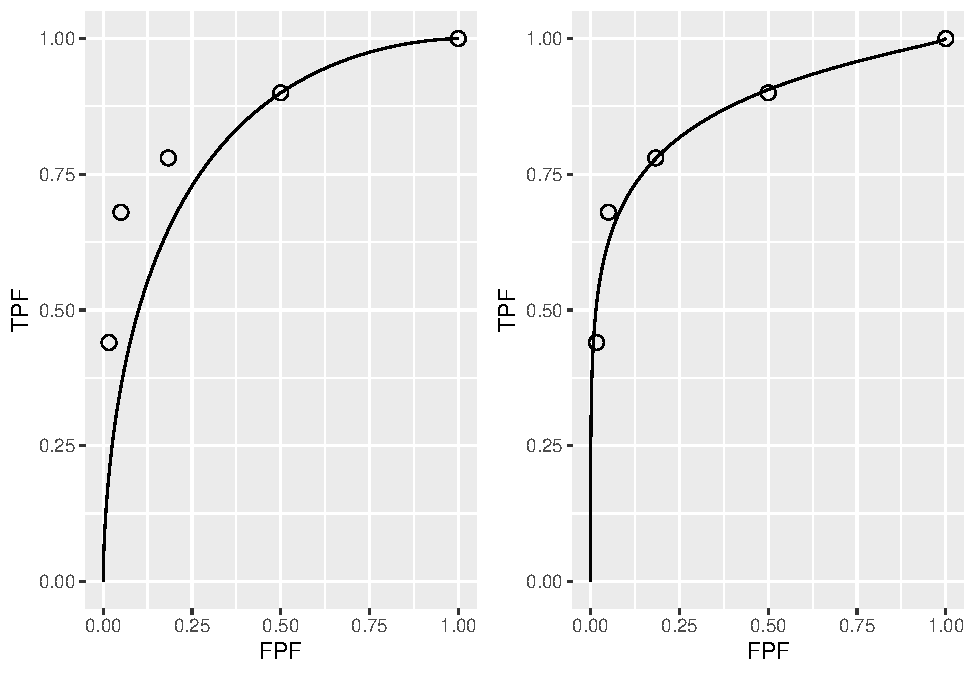
\includegraphics{04-ratings-paradigm_files/figure-latex/ratingsParadigmEqVarFitA-1.pdf}
\caption{\label{fig:ratingsParadigmEqVarFitA}The left figure is the predicted ROC curve for \(\mu=1.282\) superposed on the operating points. The right figure is the same data fitted with a two-parameter model described later.}
\end{figure}

It should come as no surprise that the uppermost operating point is \emph{exactly} on the predicted curve: after all, this point was used to calculate \(\mu\) = 2.17. The corresponding value of \(\zeta\) can be calculated from Eqn. (3.17), namely:

\begin{equation*} 
\zeta = \Phi^{-1}\left ( Sp \right )
\label{eq:ratingsParadigm-Zeta}
\end{equation*}

\begin{equation*} 
\mu = \zeta + \Phi^{-1}\left ( Se \right )
\label{eq:ratingsParadigm-Mu}
\end{equation*}

These are coded below:

\begin{Shaded}
\begin{Highlighting}[]
\KeywordTok{qnorm}\NormalTok{(}\DecValTok{1}\FloatTok{{-}0.5}\NormalTok{)}
\CommentTok{\#\textgreater{} [1] 0}
\NormalTok{mu}\OperatorTok{{-}}\KeywordTok{qnorm}\NormalTok{(}\FloatTok{0.9}\NormalTok{)}
\CommentTok{\#\textgreater{} [1] 0.888}
\end{Highlighting}
\end{Shaded}

Either way, one gets the same result: \(\zeta\) = 0. It should be clear that this makes sense: FPF = 0.5 is consistent with half of the (symmetrical) unit-normal non-diseased distribution being above \(\zeta\) = 0. The transformed value \(\zeta\) (zero in this example) is a genuine numerical value. \emph{To reiterate, ratings cannot be treated as genuine numerical values, but thresholds, estimated from an appropriate model, can be treated as genuine numerical values.}

Exercise: calculate \(\zeta\) for each of the remaining operating points. \emph{Notice that \(\zeta\) increases as one moves down the curve.}

\begin{itemize}
\item
  The ROC curve in Fig. 4.1 (A), as determined by the uppermost operating point, passes exactly through this point but misses the others. If a different operating point were used to estimate \(\mu\) = and \(A_{z;\sigma = 1}\), the estimated values would have been different and the new curve would pass exactly through the \emph{new} selected point. No single-point based choice of \(\mu\) would yield a satisfactory visual fit to all the observed operating points. {[}The reader should confirm these statements with appropriate modifications to the code.{]} * \textbf{This is the reason one needs a modified model, with an extra parameter, namely the unequal variance binormal model, to fit radiologist data} (the extra parameter is the ratio of the standard deviations of the two distributions).
\item
  Fig. 4.1 (B) shows the predicted ROC curve by the unequal variance binormal model, to be introduced in Chapter 06. The corresponding parameter values are \(\mu\) = 2.17and \(\sigma\) = 1.65.
\item
  Notice the improved visual quality of the fit. Each observed point is ``not engraved in stone'', rather both FPF and TPF are subject to sampling variability. Estimation of confidence intervals for FPF and TPF was addressed in §3.10. {[}A detail: the estimated confidence interval in the preceding chapter was for a single operating point; since the multiple operating points are correlated -- some of the counts used to calculate them are common to two or more operating points -- the method tends to overestimate the confidence interval. A modeling approach is possible to estimate confidence intervals that accounts for data correlation and this yields tighter confidence intervals.{]}
\end{itemize}

\hypertarget{relation-between-ratings-paradigm-and-the-binary-paradigm}{%
\section{Relation between ratings paradigm and the binary paradigm}\label{relation-between-ratings-paradigm-and-the-binary-paradigm}}

Table \ref{tab:ratingsParadigmTable1} and Table \ref{tab:ratingsParadigmTable2} correspond to \(R = 5\). In Chapter \ref{binaryTask0} it was shown that the binary task requires a single fixed threshold parameter \(\zeta\) and a decision or binning rule Eqn. \eqref{eq:ratingsParadigm-binningRule}: assign the case a diseased rating of 2 if \(Z > \zeta\) and a rating of 1 otherwise.

\textbf{The R-rating task can be viewed as \(R-1\) simultaneously conducted binary tasks each with its own fixed threshold \(\zeta_r\), where r = 1, 2, \ldots, R-1. It is efficient compared to \(R-1\) sequentially conducted binary tasks; however, the onus is on the observer to maintain fixed-multiple thresholds through the duration of the study.}

The rating method is a more efficient way of collecting the data compared to running the study repeatedly with appropriate instructions to cause the observer to adopt different fixed thresholds specific to each replication. In the clinical context such repeated studies would be impractical because it would introduce memory effects, wherein the diagnosis of a case would depend on how many times the case had been seen, along with other cases, in previous sessions. A second reason is that it is difficult for a radiologist to change the operating threshold in response to instructions. To the author's knowledge, repeated use of the binary paradigm has not been used in any clinical ROC study

How does one model the binning? For convenience one defines dummy thresholds \(\zeta_0 = - \infty\) and \(\zeta_R = + \infty\), in which case the thresholds satisfy the ordering requirement \(\zeta_{r-1} \le \zeta_r\) , r = 1, 2, \ldots, R. The rating or binning rule is:

\begin{equation} 
if \left (\zeta_{r-1} \le z \le \zeta_r  \right )\Rightarrow \text rating = r
\label{eq:ratingsParadigm-binningRule}
\end{equation}

For Table \ref{tab:ratingsParadigmTable2}, the \textbf{empirical} thresholds are as follows:

\begin{equation} 
\left.
\begin{aligned}
\zeta_r &= r + 1 \\
r & = 1, 2, ..., R-1\\
\zeta_0 &= -\infty\\
\zeta_R &= \infty\\
\end{aligned}
\right \}
\label{eq:ratingsParadigm-EmpZeta}
\end{equation}

The empirical thresholds are integers, as distinct from the floating point values predicted by Eqn. \eqref{eq:ratingsParadigm-Zeta}. \textbf{Either way one gets the same operating points.} This is a subtle and important distinction, which is related to the next section: one has enormous flexibility in the choice of the scale adopted for the decision variable axis.

In Table \ref{tab:ratingsParadigmTable1} the number of bins is \(R = 5\). The ``simultaneously conducted binary tasks'' nature of the rating task can be appreciated from the following examples. Suppose one selects the threshold for the first binary task to be \(\zeta_4 = 5\). By definition, \(\zeta_5 = \infty\); therefore a case rated 5 satisfies the binning rule \(\zeta_4 \leq 5 < \zeta_5\), i.e., Eqn. \eqref{eq:ratingsParadigm-binningRule}. The operating point corresponding to \(\zeta_4 = 5\), obtained by cumulating all cases rated five, yields \((0.017, 0.440)\). In the second binary-task, one selects as threshold \(\zeta_3 = 4\). Therefore, a case rated four satisfies the binning rule \(\zeta_3 \leq 4 < \zeta_4\). The operating point corresponding to \(\zeta_3 = 4\), obtained by cumulating all cases rated four or five, yields \((0.05, 0.680)\). Similarly, for \(\zeta_2 = 3\), \(\zeta_1 = 2\) and \(\zeta_0 = -\infty\), which yield counts in bins 3, 2 and 1, respectively. The last is a trivial operating point. The non-trivial operating points are generated by thresholds \(\zeta_r\), where \(r\) = 1, 2, 3 and 4. A five-rating study has four associated thresholds and a corresponding number of equivalent binary studies. In general, an \(R\) rating study has \(R-1\) associated thresholds.

\hypertarget{ratings-are-not-numerical-values}{%
\section{Ratings are not numerical values}\label{ratings-are-not-numerical-values}}

\begin{itemize}
\item
  The ratings are to be thought of as ordered labels, not as numeric values. Arithmetic operations that are allowed on numeric values, such as averaging, are not allowed on ratings. One could have relabeled the ratings in Table 4.2 as A, B, C, D and E, where A \textless{} B etc. As long as the counts in the body of the table are unaltered, such relabeling would have no effect on the observed operating points and the fitted curve. Of course one cannot average the labels A, B, etc. of different cases. The issue with numeric labels is not fundamentally different. At the root is that the difference in thresholds corresponding to the different operating points are not in relation to the difference between their numeric values. There is a way to estimate the underlying thresholds, if one assumes a specific model, for example the unequal-variance binormal model to be described in Chapter 06. The thresholds so obtained are genuine numeric values and can be averaged. {[}Not to hold the reader in suspense, the four thresholds corresponding to the data in Table 4.1 are 0.007676989, 0.8962713, 1.515645 and 2.396711; see §6.4.1; these values would be unchanged if, for example, the labels were doubled, with allowed values 2, 4, 6, 8 and 10, or any of an infinite number of rearrangements that preserves their ordering.{]}
\item
  The temptation to regard confidence levels / ratings as numeric values can be particularly strong when one uses a large number of bins to collect the data. One could use of quasi-continuous ratings scale, implemented for example, by having a slider-bar user interface for selecting the rating. The slider bar typically extends from 0 to 100, and the rating could be recorded as a floating-point number, e.g., 63.45. Here too one cannot assume that the difference between a zero-rated case and a 10 rated case is a tenth of the difference between a zero-rated case and a 100 rated case. So averaging the ratings is not allowed. Additionally, one cannot assume that different observers use the labels in the same way. One observer's 4-rating is not equivalent to another observers 4-rating. Working directly with the ratings is a bad idea: valid analytical methods use the rankings of the ratings, not their actual values. The reason for the emphasis is that there are serious misconceptions about ratings. The author is aware of a publication stating, to the effect, that a modality resulted in an increase in average confidence level for diseased cases. Another publication used a specific numerical value of a rating to calculate the operating point for each observer -- this assumes all observers use the rating scale in the same way.
\end{itemize}

\hypertarget{a-single-clinical-operating-point-from-ratings-data}{%
\section{A single ``clinical'' operating point from ratings data}\label{a-single-clinical-operating-point-from-ratings-data}}

The reason for the quotes in the title to this section is that a single operating point on a laboratory ROC plot, no matter how obtained, has little relevance to how radiologists operate in the clinic. However, some consider it useful to quote an operating point from an ROC study. For a 5-rating ROC study, Table 4.2, it is not possible to unambiguously calculate the operating point of the observer in the binary task of discriminating between non-diseased and diseased cases. One possibility would be to use the three and above ratings to define the operating point, but one might have chosen two and above. A second possibility is to instruct the radiologist that a four or higher rating, for example, implies the case would be reported ``clinically'' as diseased. However, the radiologist can only pretend so far that this study, which has no clinical consequences, is somehow a ``clinical'' study. If a single laboratory study based operating point is desired2, the best strategy , in the author's opinion, is to obtain the rating via two questions. This method is also illustrated in a book on detection theory, Ref. 3, Table 3.1. The first question is ``is the case diseased?'' The binary (Yes/No) response to this question allows unambiguous calculation of the operating point, as in Chapter 02. The second question is: ``what is your confidence in your previous decision?'' and allow three responses, namely Low, Medium and High. The dual-question approach is equivalent to a 6-point rating scale, Fig. 4.2.

\begin{itemize}
\tightlist
\item
  The ordering of the ratings can be understood as follows. The four, five and six ratings are as expected. If the radiologist states the patient is diseased and the confidence level is high that is clearly the highest end of the scale, i.e., six, and the lower confidence levels, five and four, follow, as shown. If, on the other hand, the radiologist states the patient is non-diseased, and the confidence level is high, then that must be the lowest end of the scale, i.e., ``1''. The lower confidence levels in a negative decision must be higher than ``1'', namely ``2'' and ``3'', as shown. As expected, the low confidence ratings, namely ``3'' (non-diseased, low confidence) and ``4'' (diseased, low confidence) are adjacent to each other. With this method of data-collection, there is no confusion as to what rating defines the single desired operating point as this is determined by the binary response to the first question. The 6-point rating scale is also sufficiently fine to not smooth out the ability of the radiologist to maintain distinct different levels. In the author's experience, using this scale one expects rating noise of about ±½ a rating bin, i.e., the same difficult case, shown on different occasions to the same radiologist (with sufficient time lapse or other intervening cases to minimize memory effects) is expected to elicit a ``3'' or ``4'', with roughly equal probability.
\end{itemize}

\hypertarget{observer-performance-studies-as-laboratory-simulations-of-clinical-tasks}{%
\section{Observer performance studies as laboratory simulations of clinical tasks}\label{observer-performance-studies-as-laboratory-simulations-of-clinical-tasks}}

\begin{itemize}
\item
  Observer performance paradigms (ROC, FROC, LROC and ROI) should be regarded as experiments conducted in a laboratory (i.e., controlled) setting that are intended to be representative of the actual clinical task. They should not to be confused with performance in a real ``live'' clinical setting: there is a known ``laboratory effect''22-24. For example, in one study radiologists performed better during live clinical interpretations than they did later, on the same cases, in a laboratory ROC study22. This is expected because there is more at stake during live interpretations: e.g., the patient's health and the radiologist's reputation, than during laboratory ROC studies. The claimed ``laboratory effect'' has caused some controversy. A paper25 titled ``Screening mammography: test set data can reasonably describe actual clinical reporting'' argues against the laboratory effect.
\item
  Real clinical interpretations happen every day in radiology departments all over the world. In the laboratory, the radiologist is asked to interpret the images ``as if in a clinical setting'' and render a ``diagnosis''. The laboratory decisions have no clinical consequences, e.g., the radiologist will not be sued for mistakes and their ROC study decisions have no impact on the clinical management of the patients. Usually laboratory ROC studies are conducted on retrospectively acquired images. Patients, whose images were used in an ROC study, have already been imaged in the clinic and decisions have already been made on how to manage them.
\item
  There is no guarantee that results of the laboratory study are directly applicable to clinical practice. Indeed there is an assumption that the laboratory study correlates with clinical performance. Strict equality is not required, simply that the performance in the laboratory is related monotonically to actual clinical performance. Monotonicity assures preservation of performance orderings, e.g., a radiologist has greater performance than another does or one modality is superior to another, regardless of how they are measured, in the laboratory or in the clinic. The correlation is taken to be an axiomatic truth by researchers, when in fact it is an assumption. To the extent that the participating radiologist brings his/her full clinical expertise to bear on each laboratory image interpretation, this assumption is likely to be valid.
\item
  This section provoked a strong negative response from a collaborator. To paraphrase him, "\ldots{} \emph{my friend, I think it is a pity in this book chapter you argue that these studies are simulations. I mean, the reason people perform these studies is because they believe in the results"}.
\item
  The author also believes in observer performance studies. Otherwise, he would not be writing this book. Distrust of the word ``simulation'' seems to be peculiar to this field. Simulations are widely used in ``hard'' sciences, e.g., they are used in astrophysics to determine conditions dating to 10-31 seconds after the big bang. Simulations are not to be taken lightly. Conducting clinical studies is very difficult as there are many factors not under the researcher's control. Observer performance studies of the type described in this book are the closest that one can come to the ``real thing'' and the author is a firm believer in them. These studies include key elements of the actual clinical task: the entire imaging system, radiologists (assuming the radiologist take these studies seriously in the sense of bringing their full clinical expertise to bear on each image interpretation) and real clinical images and as such are expected to correlate with real ``live'' interpretations. Proving this correlation is going to be difficult as there are many factors that complicated real interpretations. It is not clear to the author that proving or disproving this correlation is ever going to be a settled issue.
\end{itemize}

\hypertarget{discrete-vs.-continuous-ratings-the-miller-study}{%
\section{Discrete vs.~continuous ratings: the Miller study}\label{discrete-vs.-continuous-ratings-the-miller-study}}

\begin{itemize}
\item
  There is controversy about the merits of discrete vs.~continuous ratings26-28. Since the late Prof.~Charles E. Metz and the late Dr.~Robert F. Wagner have both backed the latter (i.e., continuous or quasi-continuous ratings) new ROC study designs sometimes tend to follow their advice. The author's recommendation is to follow the 6-point rating scale as outlined in Fig. 4.2. This section provides the background for the recommendation.
\item
  A widely cited (22,909 citations at the time of writing) 1954 paper by Miller29 titled ``The Magical Number Seven, Plus or Minus Two: Some Limits on Our Capacity for Processing Information'' is relevant. It is a readable paper, freely downloadable in several languages (www.musanim.com/miller1956/). In the author's judgment, this paper has not received the attention it should have in the ROC community, and for this reason portions from it are reproduced below. {[}George Armitage Miller, February 3, 1920 -- July 22, 2012, was one of the founders of the field of cognitive psychology.{]}
\item
  Miller's first objective was to comment on absolute judgments of unidimensional stimuli. Since all (univariate, i.e., single decision per case) ROC models assume a unidimensional decision variable, Miller's work is highly relevant. He comments on two papers by Pollack30,31. Pollack asked listeners to identify tones by assigning numerals to them, analogous to a rating task described above. The tones differed in frequency, covering the range 100 to 8000 Hz in equal logarithmic steps. A tone was sounded and the listener responded by giving a numeral (i.e., a rating, with higher values corresponding to higher frequencies). After the listener had made his response, he was told the correct identification of the tone. When only two or three tones were used, the listeners never confused them. With four different tones, confusions were quite rare, but with five or more tones, confusions were frequent. With fourteen different tones, the listeners made many mistakes. Since it is so succinct, the entire content of the first (1952) paper by Pollack is reproduced below:
\item
  ``In contrast to the extremely acute sensitivity of a human listener to discriminate small differences in the frequency or intensity between two sounds is his relative inability to identify (and name) sounds presented individually. When the frequency of a single tone is varied in equal‐logarithmic steps in the range between 100 cps and 8000 cps (and when the level of the tone is randomly adjusted to reduce loudness cues), the amount of information transferred is about 2.3 bits per stimulus presentation. This is equivalent to perfect identification among only 5 tones. The information transferred, under the conditions of measurement employed, is reasonably invariant under wide variations in stimulus conditions.''
\item
  By ``information'' is meant (essentially) the number of levels, measured in bits (binary digits), thereby making it independent of the unit of measurement: 1 bit corresponds to a binary rating scale, 2 bits to a four-point rating scale and 2.3 bits to 22.3 = 4.9, i.e., about 5 ratings bins. Based on Pollack's' original unpublished data, Miller put an upper limit of 2.5 bits (corresponding to about 6 ratings bins) on the amount of information that is transmitted by listeners who make absolute judgments of auditory pitch. A second paper31 by Pollack was related to: (1) the frequency range of tones; (2) the utilization of objective reference tones presented with the unknown tone; and (3) the ``dimensionality''---the number of independently varying stimulus aspects. Little additional gain in information transmission was associated with the first factor; a moderate gain was associated with the second; and a relatively substantial gain was associated with the third (we return to the dimensionality issue below).
\item
  As an interesting side-note, Miller states:
\item
  ``Most people are surprised that the number is as small as six. Of course, there is evidence that a musically sophisticated person with absolute pitch can identify accurately any one of 50 or 60 different pitches. Fortunately, I do not have time to discuss these remarkable exceptions. I say it is fortunate because I do not know how to explain their superior performance. So I shall stick to the more pedestrian fact that most of us can identify about one out of only five or six pitches before we begin to get confused.
\end{itemize}

It is interesting to consider that psychologists have been using seven-point rating scales for a long time, on the intuitive basis that trying to rate into finer categories does not really add much to the usefulness of the ratings. Pollack's results indicate that, at least for pitches, this intuition is fairly sound.

Next you can ask how reproducible this result is. Does it depend on the spacing of the tones or the various conditions of judgment? Pollack varied these conditions in a number of ways. The range of frequencies can be changed by a factor of about 20 without changing the amount of information transmitted more than a small percentage. Different groupings of the pitches decreased the transmission, but the loss was small. For example, if you can discriminate five high-pitched tones in one series and five low-pitched tones in another series, it is reasonable to expect that you could combine all ten into a single series and still tell them all apart without error. When you try it, however, it does not work. The channel capacity for pitch seems to be about six and that is the best you can do.''

\begin{itemize}
\item
  In contrast to the careful experiments conducted in the psychophysical context to elucidate this issue, the author was unable to find a single study of the number of discrete rating levels that an observer can support. Even lacking such a study, a recommendation has been made to acquire data on a quasi-continuous scale27.
\item
  There is no question that for multidimensional data, as observed in the second study by Pollack31, the observer can support more than 7 ratings bins. To quote Miller:
\item
  ``You may have noticed that I have been careful to say that this magical number seven applies to one- dimensional judgments. Everyday experience teaches us that we can identify accurately any one of several hundred faces, any one of several thousand words, any one of several thousand objects, etc. The story certainly would not be complete if we stopped at this point. We must have some understanding of why the one-dimensional variables we judge in the laboratory give results so far out of line with what we do constantly in our behavior outside the laboratory. A possible explanation lies in the number of independently variable attributes of the stimuli that are being judged. Objects, faces, words, and the like differ from one another in many ways, whereas the simple stimuli we have considered thus far differ from one another in only one respect.''
\item
  In the medical imaging context, a trivial way to increase the number of ratings would be to color-code the images: red, green and blue; now one can assign a red image rated 3, a green image rated 2, etc., which would be meaningless unless the color encoded relevant diagnostic information. Another ability, quoted in the publication27 advocating continuous ratings is the ability to recognize faces, again a multidimensional categorization task, as noted by Miller. Also quoted as an argument for continuous ratings is the ability of computer aided detection schemes that calculate many features for each perceived lesion and combine them into a single probability of malignancy, which is on a highly precise floating point 0 to 1 scale. Radiologists are not computers. Other arguments for greater number of bins: it cannot hurt and one should acquire the rating data at greater precision than the noise, especially if the radiologist is able to maintain the finer distinctions. The author worries that radiologists who are willing to go along with greater precision are over-anxious to co-operate with the experimentalist. In the author's experience, expert radiologists will not modify their reading style and one should be suspicious when overzealous radiologists accede to an investigators request to interpret images in a style that does not closely resemble the clinic. Radiologists, especially experts, do not like more than about four ratings. The author has worked with a famous chest radiologist (the late Dr.~Robert Fraser) who refused to use more than four ratings.
\item
  Another reason given for using continuous ratings is it reduces instances of data degeneracy. Data is sometimes said to be degenerate if the curve-fitting algorithm, the binormal model and the proper binormal model, cannot fit it. This occurs, for example, if there are no interior points on the ROC plot. Modifying radiologist behavior to accommodate the limitations of analytical methods seems to be inherently dubious. One could simply randomly add or subtract half an integer from the observed ratings, thereby making the rating scale more granular and reduce instances of degeneracy (this is actually done in some ROC software to overcome degeneracy issues). Another possibility is to use the empirical (trapezoidal) area under the ROC curve. This quantity can always be calculated; there are no degeneracy problems with it. Actually, fitting methods now exist that are robust to data degeneracy, such as discussed in Chapter 18 and Chapter 20, so this reason for acquiring continuous data no longer applies.
\item
  The rating task involves a unidimensional scale and the author sees no way of getting around the basic channel-limitation noted by Miller and for this reason the author recommends a 6 point scale, as in Fig. 4.2.
\item
  On the other side of the controversy it has been argued that given a large number of allowed ratings levels the observer essentially bins the data into a much smaller number of bins (e.g., 0, 20, 40, 60, 80, 100) and adds a zero-mean noise term to appear to be ``spreading out the ratings'' 35. This allows easier curve-fitting with the binormal model. However, if the intent is to get the observer to spread the ratings, so that th binormal model does not fail to fit, a better approach is to use alternate models that are very robust with respect to degneracy of the data. More on thsi later (CBM and RSM).
\end{itemize}

\hypertarget{references}{%
\section{References}\label{references}}

\hypertarget{empirical-AUC}{%
\chapter{Empirical AUC}\label{empirical-AUC}}

\hypertarget{empirical-AUC-Intro}{%
\section{Introduction}\label{empirical-AUC-Intro}}

The ROC plot, introduced in Chapter 03, is defined as the plot of sensitivity (y-axis) vs.~1-specificity (x-axis). Equivalently, it is the plot of TPF (y-axis) vs.~FPF (x-axis). An equal variance binormal model was introduced which allows an ROC plot to be fitted to a single observed operating point. In Chapter 04, the more commonly used ratings paradigm was introduced.

One of the reasons for fitting observed counts data, such as in Table 4.1 in Chapter 04, to a parametric model, is to derive analytical expressions for the separation parameter \(\mu\) of the model or the area AUC under the curve. Other figures of merit, such as the TPF at a specified FPF, or the partial area to the left of a specified FPF, can also be calculated from this model. Each figure of merit can serve as the basis for comparing two readers to determine which one is better. They have the advantage of being single values, as opposed to a pair of sensitivity-specificity values, thereby making it easier to unambiguously compare performances. Additionally, they often yield physical insight into the task, e.g., the separation parameter is the perceptual signal to noise corresponding to the diagnostic task.

It was shown, TBA Fig. 4.1 (A - B), that the equal variance binormal model did not describe a clinical dataset and that an unequal variance binormal model yielded a better visual fit. This turns out to be an almost universal finding. Before getting into the complexity of the unequal variance binormal model curve fitting, it is appropriate to introduce a simpler empirical approach, which is very popular with some researchers. The New Oxford American Dictionary definition of ``empirical'' is: ``based on, concerned with, or verifiable by observation or experience rather than theory or pure logic''. The method is also termed ``non-parametric'' as it does not involve any parametric assumptions (specifically normality assumptions). Notation is introduced for labeling individual cases that is used in subsequent chapters. An important theorem relating the empirical area under the ROC to a formal statistic, known as the Wilcoxon, is described. The importance of the theorem derives from its applications to non-parametric analysis of ROC data.

\hypertarget{empirical-ROC-plot}{%
\section{The empirical ROC plot}\label{empirical-ROC-plot}}

The empirical ROC plot is constructed by connecting adjacent observed operating points, including the trivial ones at (0,0) and (1,1), with straight lines. The trapezoidal area under this plot is a non-parametric figure of merit that is threshold independent. Since no parametric assumptions are involved, some prefer it to parametric methods, such as the one to be described in the next chapter. {[}In the context of AUC, the terms empirical, trapezoidal, or non-parametric all mean the same thing.{]}

\hypertarget{notation-for-cases}{%
\subsection{Notation for cases}\label{notation-for-cases}}

As in §3.5, cases are indexed by \(k_tt\) where \(t\) indicates the truth-status at the case (i.e., patient) level, with \(t=1\) for non diseased cases and \(t=2\) for diseased cases. Index \(k_1\) ranges from one to \(K_1\) for non-diseased cases and \(k_2\) ranges from one to \(K_2\) for diseased cases, where \(K_1\) and \(K_2\) are the total number of non-diseased and diseased cases, respectively. In Table 5.1, each case is represented as a shaded box, lighter shading for non-diseased cases and darker shading for diseased cases. There are 11 non-diseased cases, labeled N1 -- N11, in the upper row of boxes and there are seven diseased cases, labeled D1 -- D7, in the lower row of boxes.

\begin{table}

\caption{\label{tab:empirical-ROC-2index-notation}On the need for two indices to label cases in an ROC study.}
\centering
\begin{tabular}[t]{l|l|l|l|l|l|l|l|l|l|l}
\hline
 &  &  &  &  &  &  &  &  &  & \\
\hline
N1 & N2 & N3 & N4 & N5 & N6 & N7 & N8 & N9 & N10 & N11\\
\hline
D1 & D2 & D3 & D4 & D5 & D6 & D7 &  &  &  & \\
\hline
\end{tabular}
\end{table}

TBA In \ref{tab:empirical-ROC-2index-notation} the upper row shows 11 non-diseased cases, labeled N1 -- N11, while the lower row shows seven diseased cases, labeled D1 -- D7. To address any case one needs two indices: the row number \(t\) and the column number \(k_tt\). Since in general the column number depends on the value of \(t\), one needs two indices to specify the column index. To address a case one needs two indices; the first index is the row number \(t\) and the second index is the column number \(k_tt\). Since the total number of columns depends on the row number, the column index has to be t-dependent, i.e., \(k_tt\), denoting the column index \(k_t\) of a case with truth index \(t\). Alternative notation in more commonly usage uses a single index \(k\) to label the cases. It reserves the first \(K_1\) positions for non-diseased cases and the rest for diseased cases: e.g., \(k = 3\) corresponds to the third non-diseased case, \(k = K_1+5\) corresponds to the fifth diseased case, etc. Because it extends more easily to more complex data structures, e.g., FROC, I prefer the two-index notation.

\hypertarget{an-empirical-operating-point}{%
\subsection{An empirical operating point}\label{an-empirical-operating-point}}

Let \(z_{k_tt}\) represent the z-sample of case \(k_tt\). For a given reporting threshold \(\zeta\), and assuming a positive-directed rating scale (i.e., higher values correspond to greater confidence in presence of disease), empirical false positive fraction \(FPF(\zeta)\) and empirical true positive fraction \(TPF(\zeta)\) are defined by:

\begin{equation}
\left.
\begin{aligned}
FPF\left ( \zeta \right ) &= \frac{1}{K_1}\sum_{k_1=1}^{K_1}I\left ( z_{k_11} \geq \zeta \right ) \\
TPF\left ( \zeta \right ) &= \frac{1}{K_2}\sum_{k_2=1}^{K_2}I\left ( z_{k_22} \geq \zeta \right )
\end{aligned}
\right \}
\label{eq:empirical-AUC-FPF-TPF}
\end{equation}

Here \(I(x)\) is the indicator function that equals one if \(x\) is true and is zero otherwise.

In Eqn. \eqref{eq:empirical-AUC-FPF-TPF} the indicator functions act as counters, effectively counting instances where the z-sample of a case equals or exceeds \(\zeta\), and division by the appropriate denominator yields the desired left hand sides of these equations. The operating point \(O(\zeta)\) corresponding to threshold \(\zeta\) is defined by:

\begin{equation}
O\left ( \zeta \right ) = \left ( FPF\left ( \zeta \right ), TPF\left ( \zeta \right ) \right )
\label{eq:empirical-OperatingPoint}
\end{equation}

The essential difference between Eqn. \eqref{eq:empirical-AUC-FPF-TPF} and Eqn. \eqref{eq:binaryTask-FPF-TPF} is that the former is non-parametric while the latter is parametric. In TBA Chapter 03 analytical (or parametric, i.e., model parameter dependent) operating points were obtained. In contrast, here one uses the observed ratings to calculate the empirical operating point.

\hypertarget{empirical-operating-points-from-ratings-data}{%
\section{Empirical operating points from ratings data}\label{empirical-operating-points-from-ratings-data}}

Consider a ratings ROC study with \(R\) bins. Describing an R-rating empirical ROC plot requires \(R-1\) ordered empirical thresholds, see Eqn. \eqref{eq:ratingsParadigm-EmpZeta}.

The operating point \(O(\zeta_r)\) is given by:

\begin{equation}
O\left ( \zeta_r \right ) = \left ( FPF\left ( \zeta_r \right ), TPF\left ( \zeta_r \right ) \right )
\label{eq:empirical-OperatingPointZetar}
\end{equation}

Its coordinates are defined by:

\begin{equation} 
\left.
\begin{aligned}
FPF_r \equiv FPF\left ( \zeta_r \right )=\frac {1} {K_1} \sum_{k_1=1}^{K_1}I \left ( z_{k_11} \geq  \zeta_r\right ) \\
\\
TPF_r \equiv TPF\left ( \zeta_r \right )=\frac {1} {K_2} \sum_{k_2=1}^{K_2} I\left ( z_{k_22} \geq  \zeta_r\right )
\end{aligned}
\right \}
\label{eq:empirical-OperatingPointFPF-TPF-r}
\end{equation}

For example,

\begin{equation} 
\left.
\begin{aligned}
FPF_4 \equiv FPF\left ( \zeta_4 \right )=\frac {1} {K_1} \sum_{k_1=1}^{K_1}I \left ( z_{k_11} \geq  \zeta_4\right ) \\
\\
TPF_4 \equiv TPF\left ( \zeta_4 \right )=\frac {1} {K_2} \sum_{k_2=1}^{K_2} I\left ( z_{k_22} \geq  \zeta_4\right )
\\
O_4 \equiv \left ( FPF_4, TPF_4 \right ) = \left ( 0.017, 0.44 \right )\\
\\
\end{aligned}
\right \}
\label{eq:empirical-OperatingPointFPF-TPF-4}
\end{equation}

In Table \ref{tab:ratingsParadigmTable1} a sample clinical ratings data set was introduced. Shown below is a partial code listing of mainEmpRocPlot.R showing implementation of Eqn. (5.7). Except for the last statement, the plotting part of the code is suppressed.

\begin{Shaded}
\begin{Highlighting}[]
\NormalTok{K1 \textless{}{-}}\StringTok{ }\DecValTok{60}
\NormalTok{K2 \textless{}{-}}\StringTok{ }\DecValTok{50}
\NormalTok{FPF \textless{}{-}}\StringTok{ }\KeywordTok{c}\NormalTok{(}\DecValTok{0}\NormalTok{, }\KeywordTok{cumsum}\NormalTok{(}\KeywordTok{rev}\NormalTok{(}\KeywordTok{c}\NormalTok{(}\DecValTok{30}\NormalTok{, }\DecValTok{19}\NormalTok{, }\DecValTok{8}\NormalTok{, }\DecValTok{2}\NormalTok{, }\DecValTok{1}\NormalTok{))) }\OperatorTok{/}\StringTok{ }\NormalTok{K1)}
\NormalTok{TPF \textless{}{-}}\StringTok{ }\KeywordTok{c}\NormalTok{(}\DecValTok{0}\NormalTok{, }\KeywordTok{cumsum}\NormalTok{(}\KeywordTok{rev}\NormalTok{(}\KeywordTok{c}\NormalTok{(}\DecValTok{5}\NormalTok{, }\DecValTok{6}\NormalTok{, }\DecValTok{5}\NormalTok{, }\DecValTok{12}\NormalTok{, }\DecValTok{22}\NormalTok{))) }\OperatorTok{/}\StringTok{ }\NormalTok{K2)}

\NormalTok{ROCOp \textless{}{-}}\StringTok{ }\KeywordTok{data.frame}\NormalTok{(}\DataTypeTok{FPF =}\NormalTok{ FPF, }\DataTypeTok{TPF =}\NormalTok{ TPF)}
\NormalTok{ROCPlot \textless{}{-}}\StringTok{ }\KeywordTok{ggplot}\NormalTok{(}
  \DataTypeTok{data =}\NormalTok{ ROCOp, }
  \DataTypeTok{mapping =} \KeywordTok{aes}\NormalTok{(}\DataTypeTok{x =}\NormalTok{ FPF, }\DataTypeTok{y =}\NormalTok{ TPF)) }\OperatorTok{+}\StringTok{ }
\StringTok{  }\KeywordTok{geom\_line}\NormalTok{(}\DataTypeTok{size =} \DecValTok{1}\NormalTok{) }\OperatorTok{+}\StringTok{ }
\StringTok{  }\KeywordTok{geom\_point}\NormalTok{(}\DataTypeTok{size =} \DecValTok{4}\NormalTok{) }\OperatorTok{+}\StringTok{ }
\StringTok{  }\KeywordTok{theme\_bw}\NormalTok{() }\OperatorTok{+}\StringTok{ }
\StringTok{  }\KeywordTok{theme}\NormalTok{(}\DataTypeTok{panel.grid.major =} \KeywordTok{element\_blank}\NormalTok{(), }
        \DataTypeTok{panel.grid.minor =} \KeywordTok{element\_blank}\NormalTok{(), }
        \DataTypeTok{panel.border =} \KeywordTok{element\_rect}\NormalTok{(}\DataTypeTok{color =} \StringTok{"black"}\NormalTok{), }
        \DataTypeTok{axis.text =} \KeywordTok{element\_text}\NormalTok{(}\DataTypeTok{size =} \DecValTok{15}\NormalTok{), }
        \DataTypeTok{axis.title =} \KeywordTok{element\_text}\NormalTok{(}\DataTypeTok{size =} \DecValTok{20}\NormalTok{)) }\OperatorTok{+}
\StringTok{  }\KeywordTok{scale\_x\_continuous}\NormalTok{(}
    \DataTypeTok{expand =} \KeywordTok{c}\NormalTok{(}\DecValTok{0}\NormalTok{, }\DecValTok{0}\NormalTok{), }
    \DataTypeTok{breaks =} \KeywordTok{c}\NormalTok{(}\FloatTok{0.25}\NormalTok{, }\FloatTok{0.5}\NormalTok{, }\FloatTok{0.75}\NormalTok{, }\DecValTok{1}\NormalTok{)) }\OperatorTok{+}\StringTok{ }
\StringTok{  }\KeywordTok{scale\_y\_continuous}\NormalTok{(}
    \DataTypeTok{expand =} \KeywordTok{c}\NormalTok{(}\DecValTok{0}\NormalTok{, }\DecValTok{0}\NormalTok{), }\DataTypeTok{breaks =} \KeywordTok{c}\NormalTok{(}\FloatTok{0.25}\NormalTok{, }\FloatTok{0.5}\NormalTok{, }\FloatTok{0.75}\NormalTok{, }\DecValTok{1}\NormalTok{)) }\OperatorTok{+}
\StringTok{  }\KeywordTok{coord\_cartesian}\NormalTok{(}\DataTypeTok{ylim =} \KeywordTok{c}\NormalTok{(}\DecValTok{0}\NormalTok{,}\DecValTok{1}\NormalTok{), }\DataTypeTok{x =} \KeywordTok{c}\NormalTok{(}\DecValTok{0}\NormalTok{,}\DecValTok{1}\NormalTok{)) }\OperatorTok{+}\StringTok{ }
\StringTok{  }\KeywordTok{annotation\_custom}\NormalTok{(}
    \DataTypeTok{grob =} \KeywordTok{textGrob}\NormalTok{(}\KeywordTok{bquote}\NormalTok{(}\KeywordTok{italic}\NormalTok{(}\StringTok{"O"}\NormalTok{)),}
                    \DataTypeTok{gp =} \KeywordTok{gpar}\NormalTok{(}\DataTypeTok{fontsize =} \DecValTok{22}\NormalTok{)), }
    \DataTypeTok{xmin =} \FloatTok{{-}0.03}\NormalTok{, }\DataTypeTok{xmax =} \FloatTok{{-}0.03}\NormalTok{, }
    \DataTypeTok{ymin =} \FloatTok{{-}0.03}\NormalTok{, }\DataTypeTok{ymax =} \FloatTok{{-}0.03}\NormalTok{) }\OperatorTok{+}\StringTok{ }
\StringTok{  }\KeywordTok{annotation\_custom}\NormalTok{(}
    \DataTypeTok{grob =} \KeywordTok{textGrob}\NormalTok{(}\KeywordTok{bquote}\NormalTok{(}\KeywordTok{italic}\NormalTok{(O[}\DecValTok{4}\NormalTok{])),}
                    \DataTypeTok{gp =} \KeywordTok{gpar}\NormalTok{(}\DataTypeTok{fontsize =} \DecValTok{22}\NormalTok{)), }
    \DataTypeTok{xmin =} \FloatTok{0.06}\NormalTok{, }\DataTypeTok{xmax =} \FloatTok{0.06}\NormalTok{, }
    \DataTypeTok{ymin =} \FloatTok{0.40}\NormalTok{, }\DataTypeTok{ymax =} \FloatTok{0.40}\NormalTok{) }\OperatorTok{+}
\StringTok{  }\KeywordTok{annotation\_custom}\NormalTok{(}
    \DataTypeTok{grob =} \KeywordTok{textGrob}\NormalTok{(}\KeywordTok{bquote}\NormalTok{(}\KeywordTok{italic}\NormalTok{(O[}\DecValTok{3}\NormalTok{])),}
                    \DataTypeTok{gp =} \KeywordTok{gpar}\NormalTok{(}\DataTypeTok{fontsize =} \DecValTok{22}\NormalTok{)), }
    \DataTypeTok{xmin =} \FloatTok{0.10}\NormalTok{, }\DataTypeTok{xmax =} \FloatTok{0.10}\NormalTok{, }
    \DataTypeTok{ymin =} \FloatTok{0.64}\NormalTok{, }\DataTypeTok{ymax =} \FloatTok{0.64}\NormalTok{) }\OperatorTok{+}
\StringTok{  }\KeywordTok{annotation\_custom}\NormalTok{(}
    \DataTypeTok{grob =} \KeywordTok{textGrob}\NormalTok{(}\KeywordTok{bquote}\NormalTok{(}\KeywordTok{italic}\NormalTok{(O[}\DecValTok{2}\NormalTok{])),}
                    \DataTypeTok{gp =} \KeywordTok{gpar}\NormalTok{(}\DataTypeTok{fontsize =} \DecValTok{22}\NormalTok{)), }
    \DataTypeTok{xmin =} \FloatTok{0.16}\NormalTok{, }\DataTypeTok{xmax =} \FloatTok{0.16}\NormalTok{, }
    \DataTypeTok{ymin =} \FloatTok{0.83}\NormalTok{, }\DataTypeTok{ymax =} \FloatTok{0.83}\NormalTok{) }\OperatorTok{+}
\StringTok{  }\KeywordTok{annotation\_custom}\NormalTok{(}
    \DataTypeTok{grob =} \KeywordTok{textGrob}\NormalTok{(}\KeywordTok{bquote}\NormalTok{(}\KeywordTok{italic}\NormalTok{(O[}\DecValTok{1}\NormalTok{])),}
                    \DataTypeTok{gp =} \KeywordTok{gpar}\NormalTok{(}\DataTypeTok{fontsize =} \DecValTok{22}\NormalTok{)), }
    \DataTypeTok{xmin =} \FloatTok{0.49}\NormalTok{, }\DataTypeTok{xmax =} \FloatTok{0.49}\NormalTok{, }
    \DataTypeTok{ymin =} \FloatTok{0.94}\NormalTok{, }\DataTypeTok{ymax =} \FloatTok{0.94}\NormalTok{)  }

\NormalTok{p \textless{}{-}}\StringTok{ }\KeywordTok{ggplotGrob}\NormalTok{(ROCPlot)}
\NormalTok{p}\OperatorTok{$}\NormalTok{layout}\OperatorTok{$}\NormalTok{clip[p}\OperatorTok{$}\NormalTok{layout}\OperatorTok{$}\NormalTok{name}\OperatorTok{==}\StringTok{"panel"}\NormalTok{] \textless{}{-}}\StringTok{ "off"}
\KeywordTok{grid.draw}\NormalTok{(p)}
\end{Highlighting}
\end{Shaded}

\begin{figure}
\centering
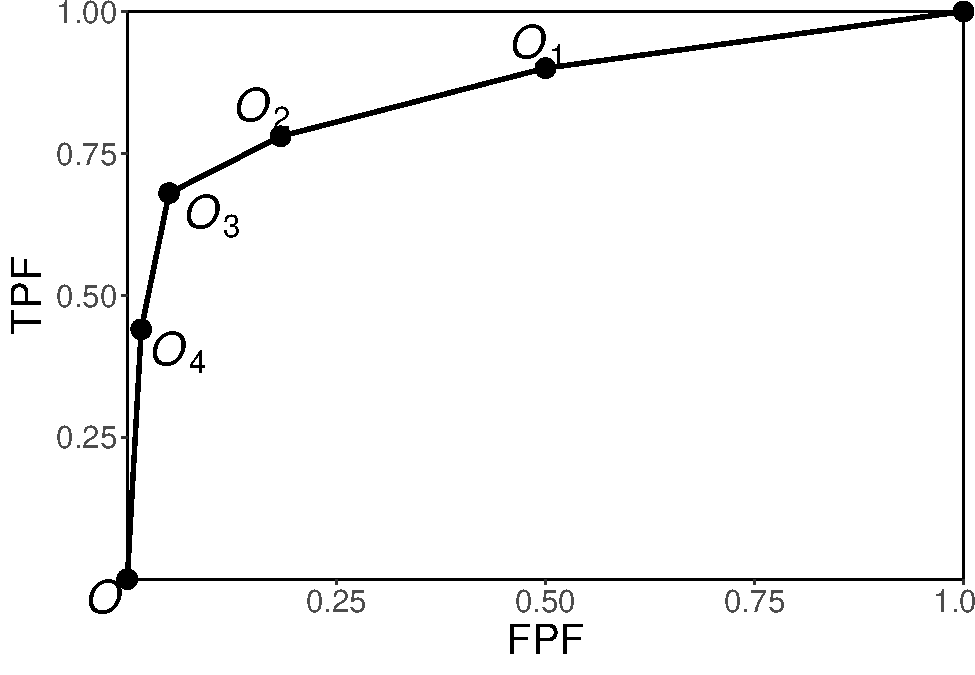
\includegraphics{05-empirical-auc_files/figure-latex/empirical-AUC-EmpiricalPlot-1.pdf}
\caption{\label{fig:empirical-AUC-EmpiricalPlot}Empirical ROC plot for the data in Table 4.1. By convention the operating points are numbered starting with the uppermost non-trivial one and working down the plot and the trivial operating points (0,0) and (1,1) are not shown.}
\end{figure}

The function \texttt{cumsum()} is used to calculate the cumulative sum. The \texttt{rev()} function reverses the order of the array supplied as its argument. The reader should use the debugging techniques (basically copy and paste parts of the code to the Console window and hit enter) to understand how this code implements Eqn. \eqref{eq:empirical-OperatingPointFPF-TPF-r}.

Fig. \ref{fig:empirical-AUC-EmpiricalPlot} is the empirical ROC plot. It illustrates the convention used to label the operating points introduced in TBA §4.3 is, i.e., \(O_1\) is the uppermost non-trivial point, and the subscripts increment by unity as one moves down the plot. By convention, not shown are the trivial operating points \(O_0 \equiv (FPF_0, TPF_0) = (1,1)\) and \(O_R \equiv (FPF_R, TPF_R) = (0,0)\), where \(R = 5\).

\hypertarget{auc-under-the-empirical-roc-plot}{%
\section{AUC under the empirical ROC plot}\label{auc-under-the-empirical-roc-plot}}

Fig. \ref{fig:empirical-AUC-EmpiricalAUC} shows the empirical plot for the data in Table 4.1. The area under the curve (AUC) is the shaded area. By dropping imaginary vertical lines from the non-trivial operating points onto the x-axis, the shaded area is seen to be the sum of one triangular shaped area and four trapezoids. One may be tempted to write equations to calculate the total area using elementary algebra, but that would be unproductive. There is a theorem (see below) that the empirical area is exactly equal to a particular statistic known as the Mann-Whitney-Wilcoxon statistic \citep{RN2191, RN2197}, which, in this book, is abbreviated to the Wilcoxon statistic. Calculating this statistic is much simpler than calculating and summing the areas of the triangle and trapezoids, or doing planimetry.

\begin{Shaded}
\begin{Highlighting}[]
\NormalTok{RocDataTable =}\StringTok{ }\KeywordTok{array}\NormalTok{(}\DataTypeTok{dim =} \KeywordTok{c}\NormalTok{(}\DecValTok{2}\NormalTok{,}\DecValTok{4}\NormalTok{))}
\NormalTok{RocDataTable[}\DecValTok{1}\NormalTok{,]  \textless{}{-}}\StringTok{ }\KeywordTok{c}\NormalTok{(}\DecValTok{30}\NormalTok{,}\DecValTok{19}\NormalTok{,}\DecValTok{8}\NormalTok{,}\DecValTok{3}\NormalTok{)}
\NormalTok{RocDataTable[}\DecValTok{2}\NormalTok{,]  \textless{}{-}}\StringTok{ }\KeywordTok{c}\NormalTok{(}\DecValTok{5}\NormalTok{,}\DecValTok{11}\NormalTok{,}\DecValTok{12}\NormalTok{,}\DecValTok{22}\NormalTok{)}

\NormalTok{ret  \textless{}{-}}\StringTok{ }\KeywordTok{RocOperatingPointsFromRatingsTable}\NormalTok{( }
\NormalTok{  RocDataTable[}\DecValTok{1}\NormalTok{,], }
\NormalTok{  RocDataTable[}\DecValTok{2}\NormalTok{,] )}
\NormalTok{FPF \textless{}{-}}\StringTok{ }\NormalTok{ret}\OperatorTok{$}\NormalTok{FPF}
\NormalTok{TPF \textless{}{-}}\StringTok{ }\NormalTok{ret}\OperatorTok{$}\NormalTok{TPF}

\NormalTok{ROC\_Points \textless{}{-}}\StringTok{ }\KeywordTok{data.frame}\NormalTok{(}\DataTypeTok{FPF =}\NormalTok{ FPF, }\DataTypeTok{TPF =}\NormalTok{ TPF)}
\CommentTok{\# add the trivial points}
\NormalTok{ROC\_Points \textless{}{-}}\StringTok{ }\KeywordTok{rbind}\NormalTok{(}
  \KeywordTok{c}\NormalTok{(}\DecValTok{0}\NormalTok{, }\DecValTok{0}\NormalTok{), }
\NormalTok{  ROC\_Points, }\KeywordTok{c}\NormalTok{(}\DecValTok{1}\NormalTok{, }\DecValTok{1}\NormalTok{))}

\NormalTok{shade \textless{}{-}}\StringTok{ }\KeywordTok{data.frame}\NormalTok{(}
  \DataTypeTok{FPF =} \KeywordTok{c}\NormalTok{(ROC\_Points}\OperatorTok{$}\NormalTok{FPF, }\DecValTok{1}\NormalTok{), }
  \DataTypeTok{TPF =} \KeywordTok{c}\NormalTok{(ROC\_Points}\OperatorTok{$}\NormalTok{TPF, }\DecValTok{0}\NormalTok{))}

\NormalTok{p \textless{}{-}}\StringTok{ }\KeywordTok{ggplot}\NormalTok{(ROC\_Points, }
            \KeywordTok{aes}\NormalTok{(}\DataTypeTok{x =}\NormalTok{ FPF, }\DataTypeTok{y =}\NormalTok{ TPF) ) }\OperatorTok{+}\StringTok{ }
\StringTok{  }\KeywordTok{geom\_polygon}\NormalTok{(}\DataTypeTok{data =}\NormalTok{ shade, }\DataTypeTok{fill =} \StringTok{\textquotesingle{}grey\textquotesingle{}}\NormalTok{) }\OperatorTok{+}\StringTok{ }
\StringTok{  }\KeywordTok{geom\_line}\NormalTok{(}\DataTypeTok{size =} \DecValTok{1}\NormalTok{) }\OperatorTok{+}\StringTok{ }
\StringTok{  }\KeywordTok{geom\_point}\NormalTok{(}\DataTypeTok{size =} \DecValTok{4}\NormalTok{) }\OperatorTok{+}\StringTok{ }
\StringTok{  }\KeywordTok{theme\_bw}\NormalTok{() }\OperatorTok{+}\StringTok{ }
\StringTok{  }\KeywordTok{theme}\NormalTok{(}
    \DataTypeTok{panel.grid.major =} \KeywordTok{element\_blank}\NormalTok{(), }
    \DataTypeTok{panel.grid.minor =} \KeywordTok{element\_blank}\NormalTok{()) }\OperatorTok{+}
\StringTok{  }\KeywordTok{labs}\NormalTok{(}\DataTypeTok{x =} \KeywordTok{expression}\NormalTok{(FPF)) }\OperatorTok{+}\StringTok{ }
\StringTok{  }\KeywordTok{labs}\NormalTok{(}\DataTypeTok{y =} \KeywordTok{expression}\NormalTok{(TPF)) }\OperatorTok{+}\StringTok{ }
\StringTok{  }\KeywordTok{scale\_x\_continuous}\NormalTok{(}\DataTypeTok{expand =} \KeywordTok{c}\NormalTok{(}\DecValTok{0}\NormalTok{, }\DecValTok{0}\NormalTok{)) }\OperatorTok{+}\StringTok{ }
\StringTok{  }\KeywordTok{scale\_y\_continuous}\NormalTok{(}\DataTypeTok{expand =} \KeywordTok{c}\NormalTok{(}\DecValTok{0}\NormalTok{, }\DecValTok{0}\NormalTok{)) }\OperatorTok{+}\StringTok{ }
\StringTok{  }\KeywordTok{coord\_cartesian}\NormalTok{(}\DataTypeTok{ylim =} \KeywordTok{c}\NormalTok{(}\DecValTok{0}\NormalTok{,}\DecValTok{1}\NormalTok{), }\DataTypeTok{x =} \KeywordTok{c}\NormalTok{(}\DecValTok{0}\NormalTok{,}\DecValTok{1}\NormalTok{))}
\KeywordTok{print}\NormalTok{(p)}
\end{Highlighting}
\end{Shaded}

\begin{figure}
\centering
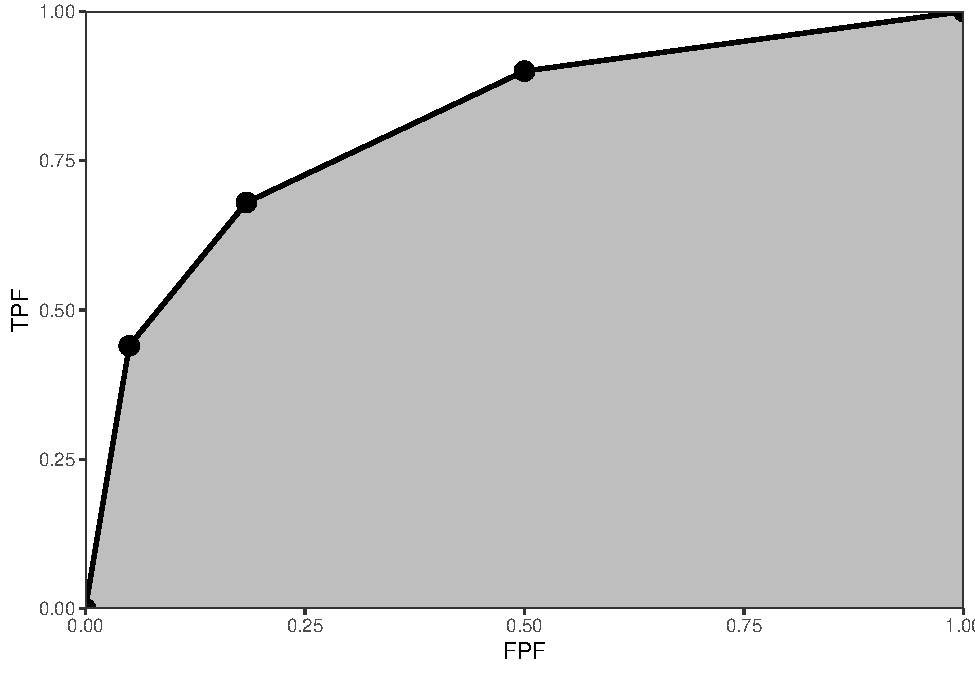
\includegraphics{05-empirical-auc_files/figure-latex/empirical-AUC-EmpiricalAUC-1.pdf}
\caption{\label{fig:empirical-AUC-EmpiricalAUC}The empirical ROC plot corresponding to Table 4.1; the shaded area is the area AUC under this plot, a widely used figure of merit in non-parametric ROC analysis.}
\end{figure}

\hypertarget{the-wilcoxon-statistic}{%
\section{The Wilcoxon statistic}\label{the-wilcoxon-statistic}}

A statistic is any value calculated from observed data. The Wilcoxon statistic is defined in terms of the ratings, by:

\begin{equation}
W=\frac{1}{K_1K_2} \sum_{k_1=1}^{K_1} \sum_{k_2=1}^{K_2} \psi\left ( z_{k_11} ,  z_{k_22} \right )
\label{eq:empirical-AUC-Wilcoxon}
\end{equation}

The function \(\psi\left ( x, y \right )\) is defined by:

\begin{equation}
\left.
\begin{aligned}
\psi(x,y)&=1  \qquad & x<y \\
\psi(x,y)&=0.5  & x=y \\
\psi(x,y)&=0  & x>y
\end{aligned}
\right \}
\label{eq:empirical-AUC-PsiFunction}
\end{equation}

The function \(\psi\left ( x, y \right )\) is sometimes called the kernel function. It is unity if the diseased case is rated higher, 0.5 if the two are rated the same and zero otherwise. Each evaluation of the kernel function results from a comparison of a case from the non-diseased set with one from the diseased set. In Eqn. \eqref{eq:empirical-AUC-Wilcoxon} the two summations and division by the total number of comparisons yields the observed, i.e., empirical, probability that diseased cases are rated higher than non-diseased ones. Since it is a probability, it can range from zero to one. However, if the observer has any discrimination ability at all, one expects diseased cases to be rated equal or greater than non-diseased ones, so in practice one expects \(0.5 \leq W \leq 1\). The limit 0.5 corresponds to a guessing observer, whose operating point lies on the chance diagonal of the ROC plot.

\hypertarget{bambers-equivalence-theorem}{%
\section{Bamber's Equivalence theorem}\label{bambers-equivalence-theorem}}

The Wilcoxon statistic \(W\) equals the area \(AUC\) under the empirical ROC plot:

\begin{equation}
W = AUC
\label{eq:empirical-AUC-BambersTheorem}
\end{equation}

Numerical illustration: While hardly a proof, as an illustration of the theorem it is helpful to calculate the sum on the right hand side of Eqn. \eqref{eq:empirical-AUC-Wilcoxon} and compare it to direct integration of the area under the empirical ROC curve (i.e., adding the area of a triangle and several trapezoids). The function is called \texttt{trapz(x,y)}, see below. It takes two array arguments, \(x\) and \(y\), where in the current case \(x\) is \(FPF\) and \(y\) is \(TPF\). One has to be careful to include the end-points as otherwise the area will be underestimated. The Wilcoxon \(W\) and the numerical estimate of the empirical area AUC are implemented in the following code.

\begin{Shaded}
\begin{Highlighting}[]
\NormalTok{trapz =}\StringTok{ }\ControlFlowTok{function}\NormalTok{(x, y)}
\NormalTok{\{ }\CommentTok{\#\#\# computes the integral of y with respect to x using trapezoidal integration.}
\NormalTok{  idx =}\StringTok{ }\DecValTok{2}\OperatorTok{:}\KeywordTok{length}\NormalTok{(x)}
  \KeywordTok{return}\NormalTok{ (}\KeywordTok{as.double}\NormalTok{( (x[idx] }\OperatorTok{{-}}\StringTok{ }\NormalTok{x[idx}\DecValTok{{-}1}\NormalTok{]) }\OperatorTok{\%*\%}\StringTok{ }\NormalTok{(y[idx] }\OperatorTok{+}\StringTok{ }\NormalTok{y[idx}\DecValTok{{-}1}\NormalTok{])) }\OperatorTok{/}\StringTok{ }\DecValTok{2}\NormalTok{)}
\NormalTok{\}}
\end{Highlighting}
\end{Shaded}

\begin{Shaded}
\begin{Highlighting}[]
\NormalTok{Wilcoxon \textless{}{-}}\StringTok{ }\ControlFlowTok{function}\NormalTok{ (zk1, zk2)}
\NormalTok{\{}
\NormalTok{  K1 =}\StringTok{ }\KeywordTok{length}\NormalTok{(zk1)}
\NormalTok{  K2 =}\StringTok{ }\KeywordTok{length}\NormalTok{(zk2)}
\NormalTok{  W \textless{}{-}}\StringTok{ }\DecValTok{0}
  \ControlFlowTok{for}\NormalTok{ (k1 }\ControlFlowTok{in} \DecValTok{1}\OperatorTok{:}\NormalTok{K1) \{}
\NormalTok{    W \textless{}{-}}\StringTok{ }\NormalTok{W }\OperatorTok{+}\StringTok{ }\KeywordTok{sum}\NormalTok{(zk1[k1] }\OperatorTok{\textless{}}\StringTok{ }\NormalTok{zk2)}
\NormalTok{    W \textless{}{-}}\StringTok{ }\NormalTok{W }\OperatorTok{+}\StringTok{ }\FloatTok{0.5} \OperatorTok{*}\StringTok{ }\KeywordTok{sum}\NormalTok{(zk1[k1] }\OperatorTok{==}\StringTok{ }\NormalTok{zk2)}
\NormalTok{  \}}
\NormalTok{  W \textless{}{-}}\StringTok{ }\NormalTok{W}\OperatorTok{/}\NormalTok{K1}\OperatorTok{/}\NormalTok{K2}
  \KeywordTok{return}\NormalTok{ (W)}
\NormalTok{\}}

\NormalTok{RocOperatingPoints \textless{}{-}}\StringTok{ }\ControlFlowTok{function}\NormalTok{( K1, K2 ) \{}
  
\NormalTok{  nOpPts \textless{}{-}}\StringTok{ }\KeywordTok{length}\NormalTok{(K1) }\OperatorTok{{-}}\StringTok{ }\DecValTok{1} \CommentTok{\# number of op points}
\NormalTok{  FPF \textless{}{-}}\StringTok{ }\KeywordTok{array}\NormalTok{(}\DecValTok{0}\NormalTok{,}\DataTypeTok{dim =}\NormalTok{ nOpPts)}
\NormalTok{  TPF \textless{}{-}}\StringTok{ }\KeywordTok{array}\NormalTok{(}\DecValTok{0}\NormalTok{,}\DataTypeTok{dim =}\NormalTok{ nOpPts)}
   
  \ControlFlowTok{for}\NormalTok{ (r }\ControlFlowTok{in}\NormalTok{ (nOpPts}\OperatorTok{+}\DecValTok{1}\NormalTok{)}\OperatorTok{:}\DecValTok{2}\NormalTok{) \{}
\NormalTok{    FPF[r}\DecValTok{{-}1}\NormalTok{] \textless{}{-}}\StringTok{ }\KeywordTok{sum}\NormalTok{(K1[r}\OperatorTok{:}\NormalTok{(nOpPts}\OperatorTok{+}\DecValTok{1}\NormalTok{)])}\OperatorTok{/}\KeywordTok{sum}\NormalTok{(K1)}
\NormalTok{    TPF[r}\DecValTok{{-}1}\NormalTok{] \textless{}{-}}\StringTok{ }\KeywordTok{sum}\NormalTok{(K2[r}\OperatorTok{:}\NormalTok{(nOpPts}\OperatorTok{+}\DecValTok{1}\NormalTok{)])}\OperatorTok{/}\KeywordTok{sum}\NormalTok{(K2)    }
\NormalTok{  \}}
\NormalTok{  FPF \textless{}{-}}\StringTok{ }\KeywordTok{rev}\NormalTok{(FPF)}
\NormalTok{  TPF \textless{}{-}}\StringTok{ }\KeywordTok{rev}\NormalTok{(TPF)}
  
  \KeywordTok{return}\NormalTok{( }\KeywordTok{list}\NormalTok{(}
    \DataTypeTok{FPF =}\NormalTok{ FPF,}
    \DataTypeTok{TPF =}\NormalTok{ TPF}
\NormalTok{  ) )}
\NormalTok{\}}
\end{Highlighting}
\end{Shaded}

\begin{Shaded}
\begin{Highlighting}[]
\NormalTok{RocCountsTable =}\StringTok{ }\KeywordTok{array}\NormalTok{(}\DataTypeTok{dim =} \KeywordTok{c}\NormalTok{(}\DecValTok{2}\NormalTok{,}\DecValTok{5}\NormalTok{))}
\NormalTok{RocCountsTable[}\DecValTok{1}\NormalTok{,]  \textless{}{-}}\StringTok{ }\KeywordTok{c}\NormalTok{(}\DecValTok{30}\NormalTok{,}\DecValTok{19}\NormalTok{,}\DecValTok{8}\NormalTok{,}\DecValTok{2}\NormalTok{,}\DecValTok{1}\NormalTok{)}
\NormalTok{RocCountsTable[}\DecValTok{2}\NormalTok{,]  \textless{}{-}}\StringTok{ }\KeywordTok{c}\NormalTok{(}\DecValTok{5}\NormalTok{,}\DecValTok{6}\NormalTok{,}\DecValTok{5}\NormalTok{,}\DecValTok{12}\NormalTok{,}\DecValTok{22}\NormalTok{)}

\NormalTok{zk1  \textless{}{-}}\StringTok{ }\KeywordTok{rep}\NormalTok{(}\DecValTok{1}\OperatorTok{:}\KeywordTok{length}\NormalTok{(RocCountsTable[}\DecValTok{1}\NormalTok{,]),RocCountsTable[}\DecValTok{1}\NormalTok{,])}\CommentTok{\#convert frequency table to array}
\NormalTok{zk2  \textless{}{-}}\StringTok{ }\KeywordTok{rep}\NormalTok{(}\DecValTok{1}\OperatorTok{:}\KeywordTok{length}\NormalTok{(RocCountsTable[}\DecValTok{2}\NormalTok{,]),RocCountsTable[}\DecValTok{2}\NormalTok{,])}\CommentTok{\#do:}

\NormalTok{w  \textless{}{-}}\StringTok{ }\KeywordTok{Wilcoxon}\NormalTok{ (zk1, zk2)}
\KeywordTok{cat}\NormalTok{(}\StringTok{"The wilcoxon statistic is = "}\NormalTok{, w, }\StringTok{"}\CharTok{\textbackslash{}n}\StringTok{"}\NormalTok{)}
\CommentTok{\#\textgreater{} The wilcoxon statistic is =  0.8606667}
\NormalTok{ret \textless{}{-}}\StringTok{ }\KeywordTok{RocOperatingPoints}\NormalTok{(RocCountsTable[}\DecValTok{1}\NormalTok{,], RocCountsTable[}\DecValTok{2}\NormalTok{,])}
\NormalTok{FPF \textless{}{-}}\StringTok{ }\NormalTok{ret}\OperatorTok{$}\NormalTok{FPF;FPF \textless{}{-}}\StringTok{ }\KeywordTok{c}\NormalTok{(}\DecValTok{0}\NormalTok{,FPF,}\DecValTok{1}\NormalTok{)}
\NormalTok{TPF \textless{}{-}}\StringTok{ }\NormalTok{ret}\OperatorTok{$}\NormalTok{TPF;TPF \textless{}{-}}\StringTok{ }\KeywordTok{c}\NormalTok{(}\DecValTok{0}\NormalTok{,TPF,}\DecValTok{1}\NormalTok{)}
\NormalTok{AUC \textless{}{-}}\StringTok{ }\KeywordTok{trapz}\NormalTok{(FPF,TPF) }\CommentTok{\# trapezoidal integration}
\KeywordTok{cat}\NormalTok{(}\StringTok{"direct integration yields AUC = "}\NormalTok{, AUC, }\StringTok{"}\CharTok{\textbackslash{}n}\StringTok{"}\NormalTok{)}
\CommentTok{\#\textgreater{} direct integration yields AUC =  0.8606667}
\end{Highlighting}
\end{Shaded}

Note the equality of the two estimates.

The following proof is adapted from \citep{RN2174} and while it may appear to be restricted to discrete ratings, the result is in fact quite general, i.e., it is applicable even if the ratings are acquired on a continuous scale. The reason is that in an R-rating ROC study the observed z-samples or ratings take on integer values, 1 through R. If R is large enough, ordering information present in the continuous data is not lost upon binning. In the following it is helpful to keep in mind that one is dealing with discrete distributions of the ratings, described by probability mass functions as opposed to probability density functions, e.g., \(P(Z_2 = \zeta_i)\) is not zero, as would be the case for continuous ratings. The proof is illustrated with Fig. \ref{fig:empirical-AUC-BambersTheorem}.

\begin{figure}
\centering
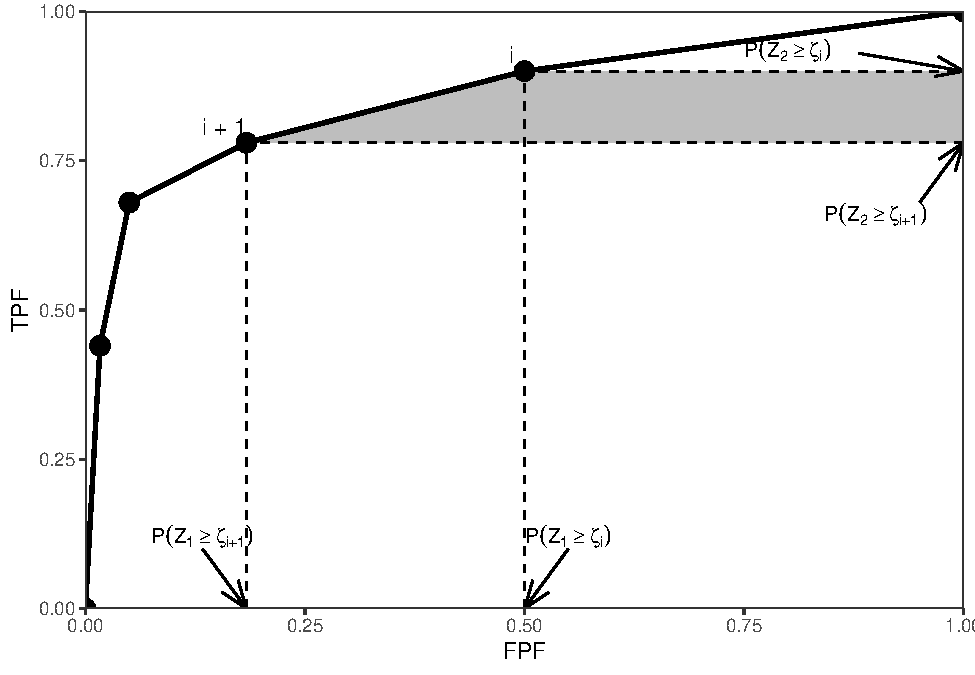
\includegraphics{05-empirical-auc_files/figure-latex/empirical-AUC-BambersTheorem-1.pdf}
\caption{\label{fig:empirical-AUC-BambersTheorem}:Illustration of the derivation of Bamber's equivalence theorem. Shows an empirical ROC plot for R = 5; the shaded area is due to points labeled i and i + 1.}
\end{figure}

The abscissa of the operating point \(i\) is \(P(Z_1 \geq \zeta_i)\) and the corresponding ordinate is \(P(Z_2 \geq \zeta_i)\). Here \(Z_1\) is a random sample from a non-diseased case and \(Z_2\) is a random sample from a diseased case. The shaded trapezoid defined by drawing horizontal lines from operating points \(i\) (upper) and \(i+1\) (lower) to the right edge of the ROC plot, Fig. \ref{fig:empirical-AUC-BambersTheorem}, has height:

\begin{equation}
P\left ( Z_2 \geq \zeta_i \right ) - P\left ( Z_2 \geq \zeta_{i+1} \right ) = P\left ( Z_2 = \zeta_i \right )
\label{eq:empirical-AUC-BambersTheoremProof1}
\end{equation}

The validity of this equation can perhaps be more easily seen when the first term is written in the form:

\begin{equation}
P\left ( Z_2 \geq \zeta_i \right ) = P\left ( Z_2 = \zeta_i \right )  + P\left ( Z_2 \geq \zeta_{i+1} \right )
\label{eq:empirical-AUC-BambersTheoremProof2}
\end{equation}

The lengths of the top and bottom edges of the trapezoid are, respectively:

\begin{equation}
1-P\left ( Z_1 \geq \zeta_i \right )=P\left ( Z_1 < \zeta_i \right )
\label{eq:empirical-AUC-BambersTheoremProof3}
\end{equation}

and

\begin{equation}
1-P\left ( Z_1 \geq \zeta_{i+1} \right )=P\left ( Z_1 < \zeta_{i+1} \right )
\label{eq:empirical-AUC-BambersTheoremProof4}
\end{equation}

The area \(A_i\) of the shaded trapezoid in Fig. \ref{fig:empirical-AUC-BambersTheorem} is (the steps are shown explicitly):

\begin{equation}
\left.
\begin{aligned}
A_i &=\frac{1}{2}P\left ( Z_2 = \zeta_i \right )\left [ P\left ( Z_1 < \zeta_i \right ) +  P\left ( Z_1 < \zeta_{i+1} \right ) \right ] \\
A_i &=P\left ( Z_2 = \zeta_i \right )\left [ \frac{1}{2}P\left ( Z_1 < \zeta_i \right ) +  \frac{1}{2} \left (P\left ( Z_1 = \zeta_i \right ) + P\left ( Z_1 < \zeta_i \right ) \right ) \right ]\\
A_i &=P\left ( Z_2 = \zeta_i \right )\left [ \frac{1}{2} P\left ( Z_1 = \zeta_i \right ) +  P\left ( Z_1 < \zeta_i \right ) \right ] \\
\end{aligned}
\right \}
\label{eq:empirical-AUC-BambersTheoremProof5}
\end{equation}

Summing over all values of \(i\), one gets for the total area under the empirical ROC plot:

\begin{equation}
\left.
\begin{aligned}
AUC & = \sum_{i=0}^{R-1}A_i\\
 & = \frac{1}{2}\sum_{i=0}^{R-1}P\left ( Z_2=\zeta_i \right )P\left ( Z_1=\zeta_i \right )+\sum_{i=0}^{R-1}P\left ( Z_2=\zeta_i \right )P\left ( Z_1<\zeta_i \right )
\end{aligned}
\right \}
\label{eq:empirical-AUC-BambersTheoremProof6}
\end{equation}

It is shown in the Appendix that the term \(A_0\) corresponds to the triangle at the upper right corner of Fig. \ref{fig:empirical-AUC-BambersTheorem}, and the term \(A_4\) corresponds to the horizontal trapezoid defined by the lowest non-trivial operating point.

Eqn. \eqref{eq:empirical-AUC-BambersTheoremProof6} can be restated as:

\begin{equation}
AUC=\frac{1}{2}P\left ( Z_1 = Z_2 \right ) + P\left ( Z_1 < Z_2 \right )
\label{eq:empirical-AUC-BambersTheoremProof7}
\end{equation}

The Wilcoxon statistic was defined in Eqn. \eqref{eq:empirical-AUC-Wilcoxon}. It can be seen that the comparisons implied by the summations and the weighting implied by the kernel function are estimating the two probabilities in the expression for in Eqn. \eqref{eq:empirical-AUC-BambersTheoremProof7}. Therefore, \(AUC = W\).

\hypertarget{importance-of-bambers-theorem}{%
\section{Importance of Bamber's theorem}\label{importance-of-bambers-theorem}}

The equivalence theorem is the starting point for all non-parametric methods of analyzing ROC plots, e.g., \citep{RN2268, RN112}. Prior to Bamber's work one knew how to plot an empirical operating characteristic and how to calculate the Wilcoxon statistic, but their equality had not been analytically proven. This was Bamber's essential contribution. In the absence of this theorem, the Wilcoxon statistic would be ``just another statistic'' in the context of ROC analysis. The theorem is so important that a major paper appeared in Radiology \citep{RN1970} devoted to the equivalence. The title of this paper was ``The meaning and use of the area under a receiver operating characteristic (ROC) curve''. The equivalence theorem literally gives meaning to the empirical area under the ROC.

\hypertarget{discussion-summary}{%
\section{Discussion / Summary}\label{discussion-summary}}

In this chapter, a simple method for estimating the area under the ROC plot has been described. The empirical AUC is a non-parametric measure of performance. Its simplicity and clear physical interpretation as the AUC under the empirical ROC (not fitted, not true) has spurred much theoretical development. These include the De Long et al method for estimating the variance of AUC of a single ROC empirical curve, and comparing pairs of ROC empirical curves5. Bamber's theorem, namely the equivalence between the empirical AUC and the Wilcoxon statistic has been derived and demonstrated.

Since the empirical AUC always yields a number, the researcher could be unaware about unusual behavior of the empirical ROC curve, so it is always a good idea to plot the data and look for evidence of large extrapolations. An example would be data points clustered at low FPF values, which imply a large AUC contribution, unsupported by intermediate operating points, from the line connecting the uppermost non-trivial operating point to (1,1).

\hypertarget{appendix-5.a-details-of-wilcoxon-theorem}{%
\section{Appendix 5.A: Details of Wilcoxon theorem}\label{appendix-5.a-details-of-wilcoxon-theorem}}

\hypertarget{upper-triangle}{%
\subsection{Upper triangle}\label{upper-triangle}}

For \(i = 0\), Eqn. \eqref{eq:empirical-AUC-BambersTheoremProof5} implies (since the lowest empirical threshold is unity, the lowest allowed rating, and there are no cases rated less than one):

\begin{equation}
\left. 
\begin{aligned}
A_0 =& P\left ( Z_2 = 1 \right )\left [ \frac{1}{2} P\left ( Z_1=1 \right ) + P\left ( Z_1<1 \right )\right ] \\
A_0 =& \frac{1}{2} P\left ( Z_1=1 \right ) P\left ( Z_2=1 \right )\\
\end{aligned}
\right \}
\end{equation}

The base of the triangle is:

\begin{equation}
1 - P\left ( Z_1 \geq 2 \right )=P\left ( Z_1 < 2 \right )=P\left ( Z_1 = 1 \right )
\end{equation}

The height of the triangle is:

\begin{equation}
1 - P\left ( Z_2 \geq 2 \right )=P\left ( Z_2 < 2 \right )=P\left ( Z_2 = 1 \right )
\end{equation}

Q.E.D.

\hypertarget{lowest-trapezoid}{%
\subsection{Lowest trapezoid}\label{lowest-trapezoid}}

For \(i = 4\), Eqn. \eqref{eq:empirical-AUC-BambersTheoremProof5} implies:

\begin{equation}
\left.
\begin{aligned}
A_4 =& P\left ( Z_2=5 \right )\left [ \frac{1}{2}P\left ( Z_1=5 \right ) + P\left ( Z_1<5 \right )\right ] \\
A_4 =& \frac{1}{2}P\left ( Z_2=5 \right )\left [ P\left ( Z_1=5 \right ) + 2P\left ( Z_1<5 \right )\right ] \\
A_4 =& \frac{1}{2}P\left ( Z_2=5 \right )\left [ P\left ( Z_1=5 \right ) +P\left ( Z_1<5 \right ) + P\left ( Z_1<5 \right )\right ] \\
A_4 =& \frac{1}{2}P\left ( Z_2=5 \right )\left [ 1 + P\left ( Z_1<5 \right )\right ] \\
\end{aligned}
\right \}
\end{equation}

The upper side of the trapezoid is

\begin{equation}
1-P\left ( Z_1 \geq 5 \right )= P\left ( Z_1 < 5 \right )
\end{equation}

The lower side is unity. The average of the two sides is:

\begin{equation}
\frac{1 + P\left ( Z_1 < 5 \right )}{2}
\end{equation}

The height is:

\begin{equation}
P\left ( Z_2 \geq 5 \right ) = P\left ( Z_2 = 5 \right )
\end{equation}

Multiplication of the last two expressions yields \(A_4\).

\hypertarget{empirical-AUC-references}{%
\section{References}\label{empirical-AUC-references}}

\hypertarget{BinMod}{%
\chapter{Binormal model}\label{BinMod}}

\hypertarget{BinModIntro}{%
\section{Introduction}\label{BinModIntro}}

In this chapter the univariate binormal model \citep{RN212} is described, in which one is dealing with one ROC rating per case, as in a single observer interpreting cases, one at a time, in a single modality. By convention the qualifier ``univariate'' is often omitted, i.e., it is implicit. In a later chapter a bivariate binormal model will be described where each case yields two ratings, as in a single observer interpreting cases in two modalities, or equivalently, two observers interpreting cases in a single modality.

The equal variance binormal model was described in Chapter ``Binary Paradigm''. The ratings method of acquiring ROC data and calculation of operating points was illustrated in Chapter ``Ratings Paradigm''. It was shown that for a clinical ROC dataset the unequal-variance binormal model fitted the data better than the equal-variance binormal model. This chapter deals with details of the unequal-variance binormal model, establishes necessary notation for describing the model, and derives expressions for sensitivity, specificity and the area under the predicted ROC curve (due to its complexity it appears in an Appendix).

The main aim of this chapter is to take the mystery out of statistical curve fitting. Accordingly, this is one chapter where the Appendices are longer than the main text, but as usual, they are essential reading as they reinforce the main text. It is not too much to expect the reader to load each file beginning with ``main'', click on Source and see what happens. {[}The reader is reminded that any file that starts with ``main'' contains directly executable code.{]}

\hypertarget{BinModTheModel}{%
\section{The binormal model}\label{BinModTheModel}}

The unequal-variance binormal model (henceforth abbreviated to binormal model; when the author means equal variances, it will be made explicit) is defined by (capital letters indicate random variables and their lower-case counterparts are actual realized values):

\begin{equation} 
Z_{k_tt}\sim N\left ( \mu_t,\sigma_{t}^{2} \right );t=1,2
\label{eq:BinModZSampling1}
\end{equation}

where

\begin{equation} 
\mu_1=0;\mu_2=\mu;\sigma_{1}^{2}=1;\sigma_{2}^{2}=\sigma^{2}
\label{eq:BinModZSampling2}
\end{equation}

Eqn. \eqref{eq:BinModZSampling1} states that the z-samples for non-diseased cases are distributed as a \(N(0,1)\) distribution, i.e., the unit normal distribution, while the z-samples for diseased cases are distributed as a \(N(\mu,\sigma^2)\) distribution, i.e., a normal distribution with mean \(\mu\) and variance \(\sigma^2\). This is a 2-parameter model of the z-samples, not counting additional threshold parameters needed for data binning.

\hypertarget{binning-the-data}{%
\subsection{Binning the data}\label{binning-the-data}}

In an R-rating ROC study the observed ratings r take on integer values, 1 through R, it being understood that higher ratings correspond to greater confidence for disease. Defining dummy cutoffs \(\zeta_0 = -\infty\) and \(\zeta_R = +\infty\), the binning rule for a case with realized z-sample z is (Chapter ``Ratings Paradigm'', Eqn. 4.13):

\begin{equation} 
if \left (\zeta_{r-1} \le z \le \zeta_r  \right )\Rightarrow \text rating = r
\label{eq:BinModZBinning}
\end{equation}

\begin{Shaded}
\begin{Highlighting}[]
\NormalTok{mu \textless{}{-}}\StringTok{ }\FloatTok{1.5}\NormalTok{;sigma \textless{}{-}}\StringTok{ }\FloatTok{1.5}

\NormalTok{z1 \textless{}{-}}\StringTok{ }\KeywordTok{seq}\NormalTok{(}\OperatorTok{{-}}\DecValTok{3}\NormalTok{, }\DecValTok{4}\NormalTok{, }\DataTypeTok{by =} \FloatTok{0.01}\NormalTok{)}
\NormalTok{z2 \textless{}{-}}\StringTok{ }\KeywordTok{seq}\NormalTok{(}\OperatorTok{{-}}\DecValTok{3}\NormalTok{, }\DecValTok{6}\NormalTok{, }\DataTypeTok{by =} \FloatTok{0.01}\NormalTok{)}

\NormalTok{Pdf1 \textless{}{-}}\StringTok{ }\KeywordTok{dnorm}\NormalTok{(z1)}
\NormalTok{Pdf2 \textless{}{-}}\StringTok{ }\KeywordTok{dnorm}\NormalTok{(z2, mu, }\DataTypeTok{sd =}\NormalTok{ sigma)}

\NormalTok{df \textless{}{-}}\StringTok{ }\KeywordTok{data.frame}\NormalTok{(}\DataTypeTok{z =} \KeywordTok{c}\NormalTok{(z1, z2), }\DataTypeTok{pdfs =} \KeywordTok{c}\NormalTok{(Pdf1, Pdf2), }
                 \DataTypeTok{truth =} 
                   \KeywordTok{c}\NormalTok{(}\KeywordTok{rep}\NormalTok{(}\StringTok{\textquotesingle{}non{-}diseased\textquotesingle{}}\NormalTok{, }
                         \KeywordTok{length}\NormalTok{(Pdf1)), }
                     \KeywordTok{rep}\NormalTok{(}\StringTok{\textquotesingle{}diseased\textquotesingle{}}\NormalTok{, }\KeywordTok{length}\NormalTok{(Pdf2))), }
                 \DataTypeTok{stringsAsFactors =} \OtherTok{FALSE}\NormalTok{)}

\NormalTok{cut\_point \textless{}{-}}\StringTok{ }\KeywordTok{data.frame}\NormalTok{(}\DataTypeTok{z =} \KeywordTok{c}\NormalTok{(}\OperatorTok{{-}}\FloatTok{2.0}\NormalTok{, }\FloatTok{{-}0.5}\NormalTok{, }\DecValTok{1}\NormalTok{, }\FloatTok{2.5}\NormalTok{))}

\NormalTok{rocPdfs \textless{}{-}}\StringTok{ }\KeywordTok{ggplot}\NormalTok{(df, }\KeywordTok{aes}\NormalTok{(}\DataTypeTok{x =}\NormalTok{ z, }\DataTypeTok{y =}\NormalTok{ pdfs, }\DataTypeTok{color =}\NormalTok{ truth)) }\OperatorTok{+}\StringTok{ }
\StringTok{  }\KeywordTok{geom\_line}\NormalTok{(}\DataTypeTok{size =} \DecValTok{1}\NormalTok{) }\OperatorTok{+}\StringTok{ }
\StringTok{  }\KeywordTok{scale\_colour\_manual}\NormalTok{(}\DataTypeTok{values=}\KeywordTok{c}\NormalTok{(}\StringTok{"darkgrey"}\NormalTok{,}\StringTok{"black"}\NormalTok{)) }\OperatorTok{+}\StringTok{ }
\StringTok{  }\KeywordTok{theme}\NormalTok{(}
    \DataTypeTok{legend.title =} \KeywordTok{element\_blank}\NormalTok{(), }
    \DataTypeTok{legend.position =} \KeywordTok{c}\NormalTok{(}\FloatTok{0.85}\NormalTok{, }\FloatTok{0.90}\NormalTok{), }
    \DataTypeTok{legend.text =} \KeywordTok{element\_text}\NormalTok{(}\DataTypeTok{face =} \StringTok{"bold"}\NormalTok{), }
    \DataTypeTok{axis.title.x =} \KeywordTok{element\_text}\NormalTok{(}\DataTypeTok{hjust =} \FloatTok{0.8}\NormalTok{, }\DataTypeTok{size =} \DecValTok{14}\NormalTok{,}\DataTypeTok{face=}\StringTok{"bold"}\NormalTok{),}
    \DataTypeTok{axis.title.y =} \KeywordTok{element\_text}\NormalTok{(}\DataTypeTok{size =} \DecValTok{14}\NormalTok{,}\DataTypeTok{face=}\StringTok{"bold"}\NormalTok{)) }\OperatorTok{+}
\StringTok{  }\KeywordTok{geom\_vline}\NormalTok{(}\DataTypeTok{data =}\NormalTok{ cut\_point, }\KeywordTok{aes}\NormalTok{(}\DataTypeTok{xintercept =}\NormalTok{ z), }
             \DataTypeTok{linetype =} \StringTok{"dashed"}\NormalTok{, }\DataTypeTok{size =} \FloatTok{0.25}\NormalTok{) }\OperatorTok{+}
\StringTok{  }\KeywordTok{annotation\_custom}\NormalTok{(}
    \DataTypeTok{grob =} 
      \KeywordTok{textGrob}\NormalTok{(}\KeywordTok{bquote}\NormalTok{(}\KeywordTok{italic}\NormalTok{(}\StringTok{"O"}\NormalTok{)),}
               \DataTypeTok{gp =} \KeywordTok{gpar}\NormalTok{(}\DataTypeTok{fontsize =} \DecValTok{12}\NormalTok{)), }
    \DataTypeTok{xmin =} \FloatTok{{-}3.2}\NormalTok{, }\DataTypeTok{xmax =} \FloatTok{{-}3.2}\NormalTok{, }\CommentTok{\# adjust the position of "O"}
    \DataTypeTok{ymin =} \FloatTok{{-}0.0}\NormalTok{, }\DataTypeTok{ymax =} \FloatTok{{-}0.01}\NormalTok{) }\OperatorTok{+}
\StringTok{  }\KeywordTok{scale\_x\_continuous}\NormalTok{(}\DataTypeTok{expand =} \KeywordTok{c}\NormalTok{(}\DecValTok{0}\NormalTok{, }\DecValTok{0}\NormalTok{)) }\OperatorTok{+}\StringTok{ }
\StringTok{  }\KeywordTok{scale\_y\_continuous}\NormalTok{(}\DataTypeTok{expand =} \KeywordTok{c}\NormalTok{(}\DecValTok{0}\NormalTok{, }\DecValTok{0}\NormalTok{),}\DataTypeTok{limits=}\KeywordTok{c}\NormalTok{(}\OtherTok{NA}\NormalTok{,}\FloatTok{0.4}\NormalTok{))}

\ControlFlowTok{for}\NormalTok{ (i }\ControlFlowTok{in} \DecValTok{1} \OperatorTok{:}\StringTok{ }\KeywordTok{length}\NormalTok{(cut\_point}\OperatorTok{$}\NormalTok{z))\{}
\NormalTok{  rocPdfs \textless{}{-}}\StringTok{ }\NormalTok{rocPdfs }\OperatorTok{+}
\StringTok{    }\KeywordTok{annotation\_custom}\NormalTok{(}
      \DataTypeTok{grob =} 
        \KeywordTok{textGrob}\NormalTok{(}\KeywordTok{bquote}\NormalTok{(zeta[.(i)]),}\DataTypeTok{gp =} \KeywordTok{gpar}\NormalTok{(}\DataTypeTok{fontsize =} \DecValTok{12}\NormalTok{)),}
      \DataTypeTok{xmin =}\NormalTok{ cut\_point}\OperatorTok{$}\NormalTok{z[i], }\DataTypeTok{xmax =}\NormalTok{ cut\_point}\OperatorTok{$}\NormalTok{z[i],}
      \DataTypeTok{ymin =} \FloatTok{{-}0.025}\NormalTok{, }\DataTypeTok{ymax =} \FloatTok{{-}0.045}\NormalTok{)}
\NormalTok{\}}

\NormalTok{gt \textless{}{-}}\StringTok{ }\KeywordTok{ggplot\_gtable}\NormalTok{(}\KeywordTok{ggplot\_build}\NormalTok{(rocPdfs))}
\NormalTok{gt}\OperatorTok{$}\NormalTok{layout}\OperatorTok{$}\NormalTok{clip[gt}\OperatorTok{$}\NormalTok{layout}\OperatorTok{$}\NormalTok{name }\OperatorTok{==}\StringTok{ "panel"}\NormalTok{] \textless{}{-}}\StringTok{ "off"}
\KeywordTok{grid.draw}\NormalTok{(gt)}
\end{Highlighting}
\end{Shaded}

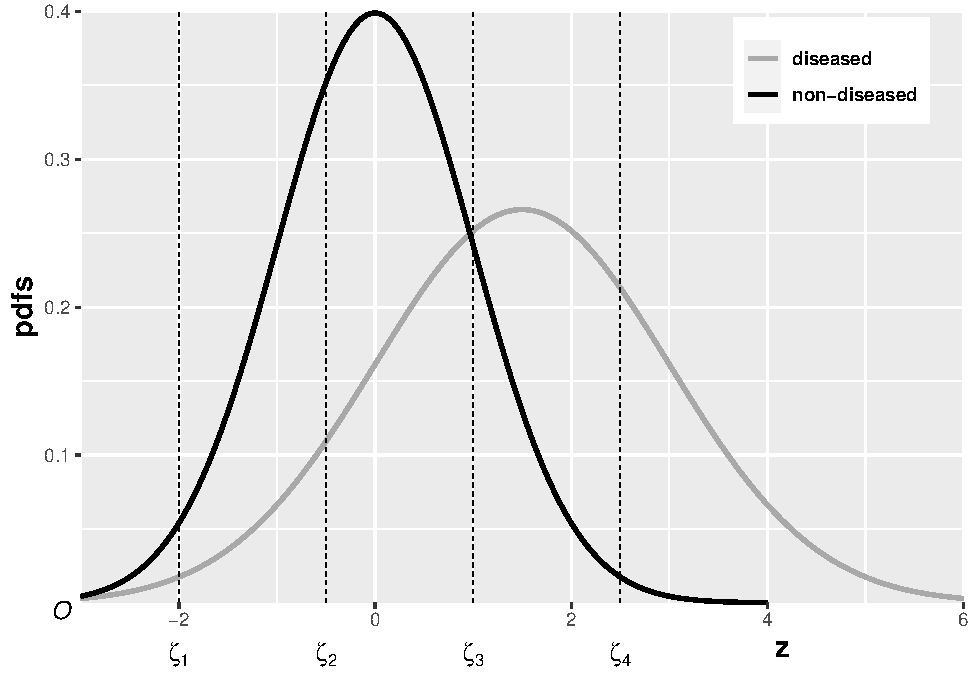
\includegraphics{06-binormal-model_files/figure-latex/unnamed-chunk-2-1.pdf}

In the unequal-variance binormal model, the variance \(\sigma^2\) of the z-samples for diseased cases is allowed to be different from unity. Most ROC datasets are consistent with \(\sigma > 1\). The above figure, generated with \(\mu = 1.5, \sigma = 1.5\), illustrates how realized z-samples are converted to ratings, i.e., application of the binning rule. For example, a case with z-sample equal to -2.5 would be rated ``1'', and one with z-sample equal to -1 would be rated ``2'', cases with z-samples greater than 2.5 would be rated ``5'', etc.

\hypertarget{invariance-of-the-binormal-model-to-arbitrary-monotone-transformations}{%
\subsection{Invariance of the binormal model to arbitrary monotone transformations}\label{invariance-of-the-binormal-model-to-arbitrary-monotone-transformations}}

The binormal model is not as restrictive as might appear at first sight. Any monotone increasing transformation \(Y=f(Z)\) applied to the observed z-samples, and the associated thresholds, will yield the same observed data, e.g., Table 6.1. This is because such a transformation leaves the ordering of the ratings unaltered and hence results in the same operating points. While the distributions for will not be binormal (i.e., two independent normal distributions), one can safely ``pretend'' that one is still dealing with an underlying binormal model. An alternative way of stating this is that any pair of distributions is allowed as long as they are reducible to a binormal model form by a monotonic increasing transformation of Y: e.g., \(Z=f^{-1}\). {[}If \(f\) is a monotone increasing function of its argument, so is \(f^{-1}\)\}.{]} For this reason, the term ``pair of latent underlying normal distributions'' is sometimes used to describe the binormal model. The robustness of the binormal model has been investigated \citep{RN1216, RN100}. The referenced paper by Dorfman et al has an excellent discussion of the robustness of the binormal model.

The robustness of the binormal model, i.e., the flexibility allowed by the infinite choices of monotonic increasing functions, application of each of which leaves the ordering of the data unaltered, is widely misunderstood. The non-Gaussian appearance of histograms of ratings in ROC studies can lead one to incorrect conclusions that the binormal model is inapplicable to these datasets. To quote a reviewer of one of the author's recent papers:
\textgreater{} I have had multiple encounters with statisticians who do not understand this difference\ldots. They show me histograms of data, and tell me that the data is obviously not normal, therefore the binormal model should not be used.

The reviewer is correct. The misconception is illustrated next.

\begin{Shaded}
\begin{Highlighting}[]
\CommentTok{\# shows that monotone transformations have no effect on }
\CommentTok{\# AUC even though the pdfs look non{-}gaussian}
\CommentTok{\# common statistician misconception about ROC analysis}

\KeywordTok{options}\NormalTok{(}\DataTypeTok{digits =} \DecValTok{7}\NormalTok{) }\CommentTok{\# line 10}

\NormalTok{fArray \textless{}{-}}\StringTok{ }\KeywordTok{c}\NormalTok{(}\FloatTok{0.1}\NormalTok{,}\FloatTok{0.5}\NormalTok{,}\FloatTok{0.9}\NormalTok{);seedArray \textless{}{-}}\StringTok{ }\KeywordTok{c}\NormalTok{(}\DecValTok{10}\NormalTok{,}\DecValTok{11}\NormalTok{,}\DecValTok{12}\NormalTok{)}
\ControlFlowTok{for}\NormalTok{ (i }\ControlFlowTok{in} \DecValTok{1}\OperatorTok{:}\DecValTok{3}\NormalTok{) \{ }
\NormalTok{  f \textless{}{-}}\StringTok{ }\NormalTok{fArray[i];seed \textless{}{-}}\StringTok{ }\NormalTok{seedArray[i];}\KeywordTok{set.seed}\NormalTok{(seed) }\CommentTok{\# line 20}
\NormalTok{  K1 \textless{}{-}}\StringTok{ }\DecValTok{900}
\NormalTok{  K2 \textless{}{-}}\StringTok{ }\DecValTok{1000}
\NormalTok{  mu1 \textless{}{-}}\StringTok{ }\DecValTok{30}
\NormalTok{  sigma1 \textless{}{-}}\StringTok{ }\DecValTok{7}
\NormalTok{  mu2 \textless{}{-}}\StringTok{ }\DecValTok{55}\NormalTok{;sigma2 \textless{}{-}}\StringTok{ }\DecValTok{7} \CommentTok{\# line 21}
\NormalTok{  z1 \textless{}{-}}\StringTok{ }\KeywordTok{rnorm}\NormalTok{(}
\NormalTok{    K1, }
    \DataTypeTok{mean =}\NormalTok{ mu1, }
    \DataTypeTok{sd =}\NormalTok{ sigma1)}
\NormalTok{  z1[z1}\OperatorTok{\textgreater{}}\DecValTok{100}\NormalTok{] \textless{}{-}}\StringTok{ }\DecValTok{100}\NormalTok{;z1[z1}\OperatorTok{\textless{}}\DecValTok{0}\NormalTok{] \textless{}{-}}\StringTok{ }\DecValTok{0}
\NormalTok{  z2 \textless{}{-}}\StringTok{ }\KeywordTok{rnorm}\NormalTok{(}
\NormalTok{    K2, }
    \DataTypeTok{mean =}\NormalTok{ mu2, }
    \DataTypeTok{sd =}\NormalTok{ sigma2)}
\NormalTok{  z2[z2}\OperatorTok{\textgreater{}}\DecValTok{100}\NormalTok{] \textless{}{-}}\StringTok{ }\DecValTok{100}\NormalTok{;z2[z2}\OperatorTok{\textless{}}\DecValTok{0}\NormalTok{] \textless{}{-}}\StringTok{ }\DecValTok{0}
\NormalTok{  AUC1 \textless{}{-}}\StringTok{ }\KeywordTok{TrapezoidalArea}\NormalTok{(z1, z2)}
\NormalTok{  Gaussians \textless{}{-}}\StringTok{ }\KeywordTok{c}\NormalTok{(z1, z2)}
\NormalTok{  hist1 \textless{}{-}}\StringTok{ }\KeywordTok{data.frame}\NormalTok{(}\DataTypeTok{x=}\NormalTok{Gaussians) }\CommentTok{\#  line 27}
\NormalTok{  hist}\FloatTok{.1}\NormalTok{ \textless{}{-}}\StringTok{  }
\StringTok{    }\KeywordTok{ggplot}\NormalTok{(}\DataTypeTok{data =}\NormalTok{ hist1, }\DataTypeTok{mapping =} \KeywordTok{aes}\NormalTok{(}\DataTypeTok{x =}\NormalTok{ x)) }\OperatorTok{+}
\StringTok{    }\KeywordTok{geom\_histogram}\NormalTok{(}\DataTypeTok{binwidth =} \DecValTok{5}\NormalTok{, }\DataTypeTok{color =} \StringTok{"black"}\NormalTok{, }\DataTypeTok{fill=}\StringTok{"grey"}\NormalTok{) }\OperatorTok{+}\StringTok{ }
\StringTok{    }\KeywordTok{xlab}\NormalTok{(}\DataTypeTok{label =} \StringTok{"Original Rating"}\NormalTok{) }\OperatorTok{+}\StringTok{ }
\StringTok{    }\KeywordTok{ggtitle}\NormalTok{(}\DataTypeTok{label =} \KeywordTok{paste0}\NormalTok{(}\StringTok{"A"}\NormalTok{, i, }\StringTok{": "}\NormalTok{, }\StringTok{"Gaussians"}\NormalTok{))}
  \KeywordTok{print}\NormalTok{(hist}\FloatTok{.1}\NormalTok{)}
  
\NormalTok{  z \textless{}{-}}\StringTok{ }\KeywordTok{seq}\NormalTok{(}\FloatTok{0.0}\NormalTok{, }\DecValTok{100}\NormalTok{, }\FloatTok{0.1}\NormalTok{) }\CommentTok{\# line 32}
\NormalTok{  curveData \textless{}{-}}\StringTok{ }
\StringTok{    }\KeywordTok{data.frame}\NormalTok{(}\DataTypeTok{x =}\NormalTok{ z, }
               \DataTypeTok{z =}  \KeywordTok{Y}\NormalTok{(z,mu1,mu2,sigma1,sigma2,f))}
\NormalTok{  plot3 \textless{}{-}}\StringTok{ }
\StringTok{    }\KeywordTok{ggplot}\NormalTok{(}\DataTypeTok{mapping =} \KeywordTok{aes}\NormalTok{(}\DataTypeTok{x =}\NormalTok{ x, }\DataTypeTok{y =}\NormalTok{ z)) }\OperatorTok{+}\StringTok{ }
\StringTok{    }\KeywordTok{geom\_line}\NormalTok{(}\DataTypeTok{data =}\NormalTok{ curveData, }\DataTypeTok{size =} \DecValTok{1}\NormalTok{) }\OperatorTok{+}
\StringTok{    }\KeywordTok{xlab}\NormalTok{(}\DataTypeTok{label =} \StringTok{"Original Rating"}\NormalTok{) }\OperatorTok{+}
\StringTok{    }\KeywordTok{ylab}\NormalTok{(}\DataTypeTok{label =} \StringTok{"Transformed Rating"}\NormalTok{) }\OperatorTok{+}\StringTok{ }
\StringTok{    }\KeywordTok{ggtitle}\NormalTok{(}
      \DataTypeTok{label =} \KeywordTok{paste0}\NormalTok{(}\StringTok{"B"}\NormalTok{, i, }\StringTok{": "}\NormalTok{, }
                     \StringTok{"Monotone Transformation"}\NormalTok{))}
  \KeywordTok{print}\NormalTok{(plot3)}
  
\NormalTok{  y \textless{}{-}}\StringTok{ }\KeywordTok{Y}\NormalTok{(}\KeywordTok{c}\NormalTok{(z1, z2),mu1,mu2,sigma1,sigma2,f)}
\NormalTok{  y1 \textless{}{-}}\StringTok{ }\NormalTok{y[}\DecValTok{1}\OperatorTok{:}\NormalTok{K1];y2 \textless{}{-}}\StringTok{ }\NormalTok{y[(K1}\OperatorTok{+}\DecValTok{1}\NormalTok{)}\OperatorTok{:}\NormalTok{(K1}\OperatorTok{+}\NormalTok{K2)]}
\NormalTok{  AUC2 \textless{}{-}}\StringTok{ }\KeywordTok{TrapezoidalArea}\NormalTok{( y1, y2)}
\NormalTok{  hist2 \textless{}{-}}\StringTok{ }\KeywordTok{data.frame}\NormalTok{(}\DataTypeTok{x=}\NormalTok{y)}
\NormalTok{  hist}\FloatTok{.2}\NormalTok{ \textless{}{-}}\StringTok{  }\KeywordTok{ggplot}\NormalTok{(}\DataTypeTok{data =}\NormalTok{ hist2, }\DataTypeTok{mapping =} \KeywordTok{aes}\NormalTok{(}\DataTypeTok{x =}\NormalTok{ x)) }\OperatorTok{+}
\StringTok{    }\KeywordTok{geom\_histogram}\NormalTok{(}\DataTypeTok{binwidth =} \DecValTok{5}\NormalTok{, }\DataTypeTok{color =} \StringTok{"black"}\NormalTok{, }\DataTypeTok{fill=}\StringTok{"grey"}\NormalTok{) }\OperatorTok{+}
\StringTok{    }\KeywordTok{xlab}\NormalTok{(}\DataTypeTok{label =} \StringTok{"Transformed Rating"}\NormalTok{) }\OperatorTok{+}\StringTok{ }
\StringTok{    }\KeywordTok{ggtitle}\NormalTok{(}
      \DataTypeTok{label =} \KeywordTok{paste0}\NormalTok{(}\StringTok{"C"}\NormalTok{, i, }\StringTok{": "}\NormalTok{, }\StringTok{"Latent Gaussians"}\NormalTok{))}
  \KeywordTok{print}\NormalTok{(hist}\FloatTok{.2}\NormalTok{)}
  \KeywordTok{cat}\NormalTok{(}\StringTok{"seed ="}\NormalTok{, seed, }\StringTok{"f ="}\NormalTok{, f, }
      \StringTok{"}\CharTok{\textbackslash{}n}\StringTok{AUC of actual Gaussians ="}\NormalTok{, AUC1, }
      \StringTok{"}\CharTok{\textbackslash{}n}\StringTok{AUC of latent Gaussians ="}\NormalTok{, AUC2, }\StringTok{"}\CharTok{\textbackslash{}n}\StringTok{"}\NormalTok{)}
\NormalTok{\}}
\CommentTok{\#\textgreater{} seed = 10 f = 0.1 }
\CommentTok{\#\textgreater{} AUC of actual Gaussians = 0.99308 }
\CommentTok{\#\textgreater{} AUC of latent Gaussians = 0.99308}
\CommentTok{\#\textgreater{} seed = 11 f = 0.5 }
\CommentTok{\#\textgreater{} AUC of actual Gaussians = 0.9936689 }
\CommentTok{\#\textgreater{} AUC of latent Gaussians = 0.9936689}
\CommentTok{\#\textgreater{} seed = 12 f = 0.9 }
\CommentTok{\#\textgreater{} AUC of actual Gaussians = 0.9950411 }
\CommentTok{\#\textgreater{} AUC of latent Gaussians = 0.9950411}
\end{Highlighting}
\end{Shaded}

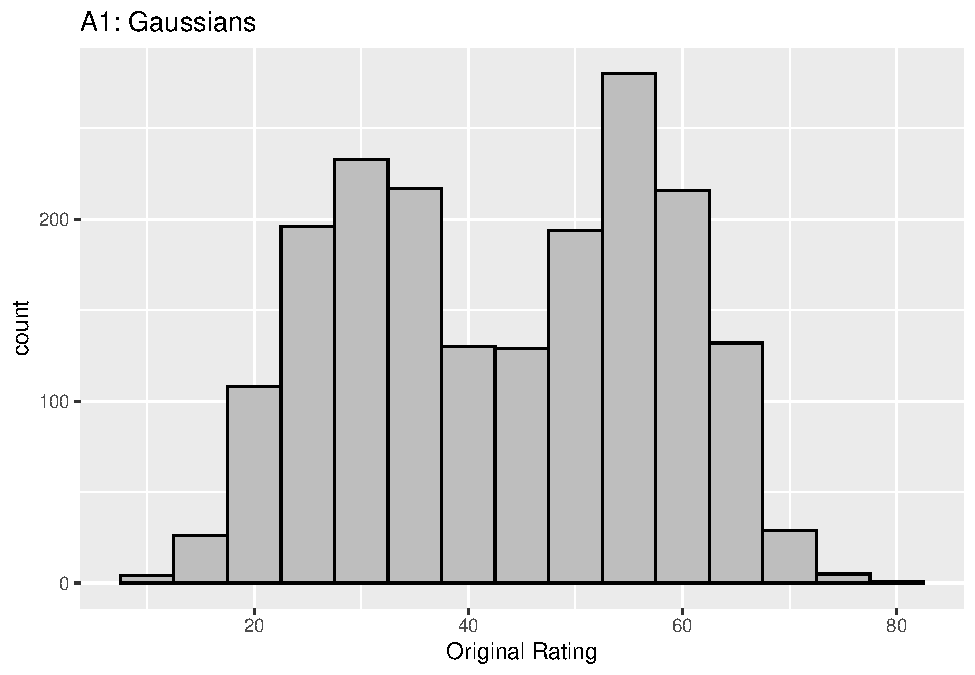
\includegraphics[width=0.33\linewidth]{06-binormal-model_files/figure-latex/unnamed-chunk-4-1} 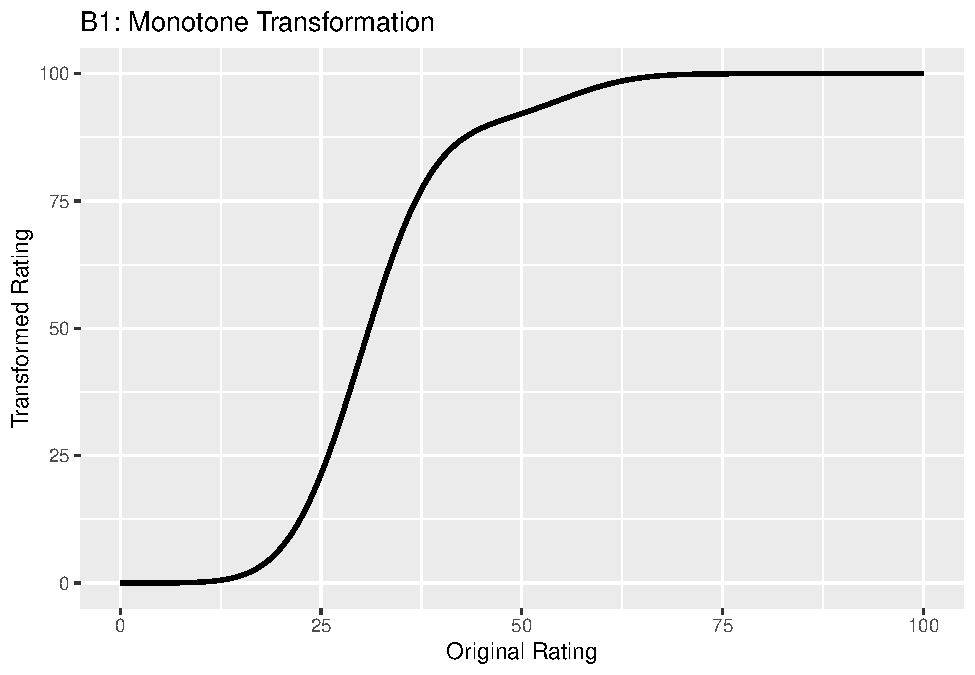
\includegraphics[width=0.33\linewidth]{06-binormal-model_files/figure-latex/unnamed-chunk-4-2} 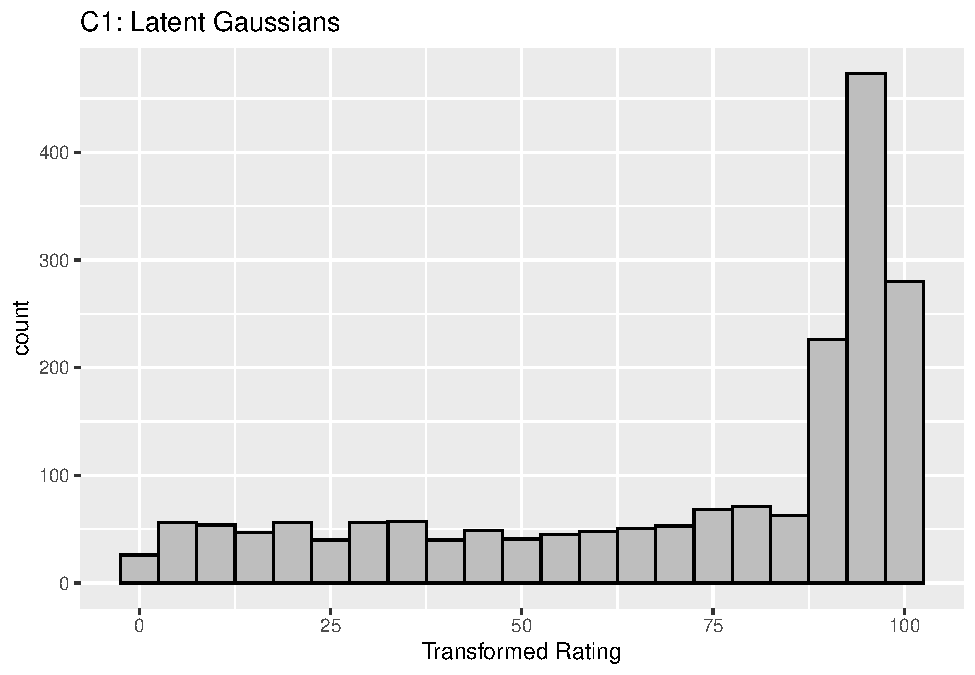
\includegraphics[width=0.33\linewidth]{06-binormal-model_files/figure-latex/unnamed-chunk-4-3} 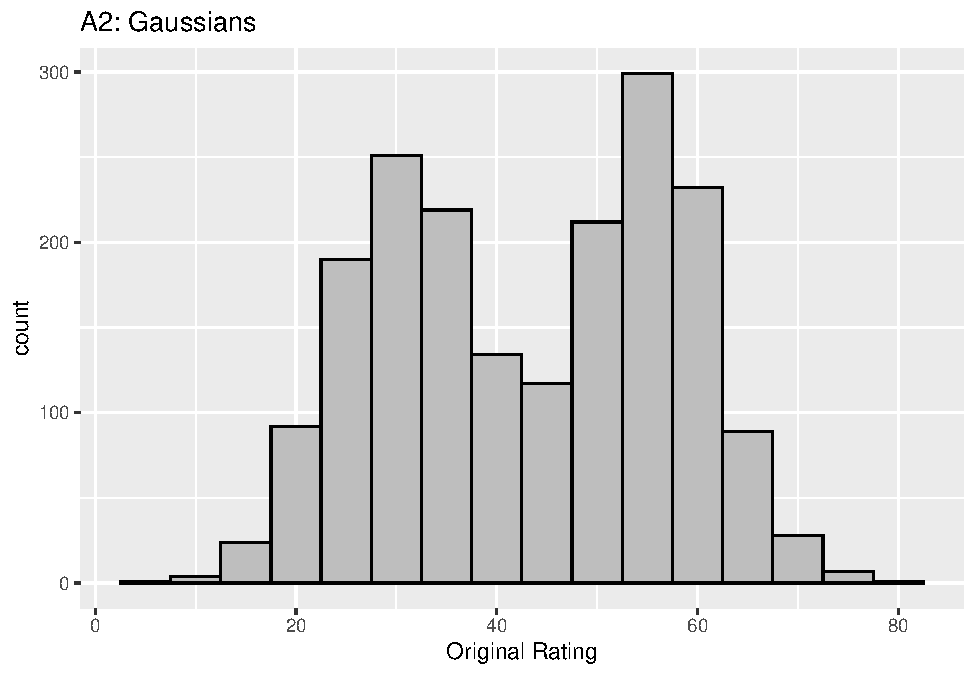
\includegraphics[width=0.33\linewidth]{06-binormal-model_files/figure-latex/unnamed-chunk-4-4} 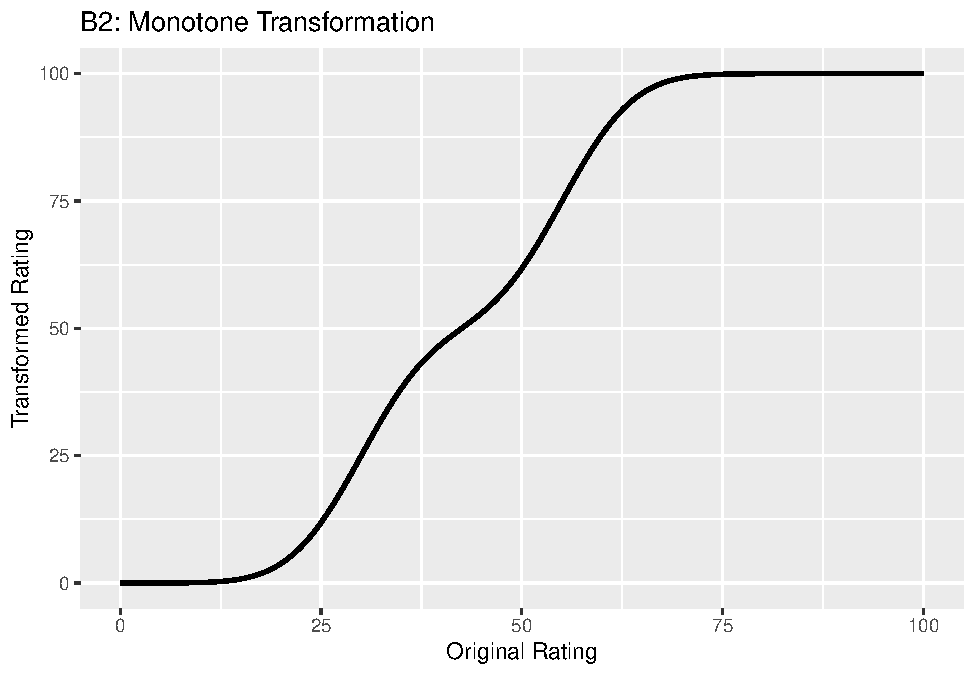
\includegraphics[width=0.33\linewidth]{06-binormal-model_files/figure-latex/unnamed-chunk-4-5} 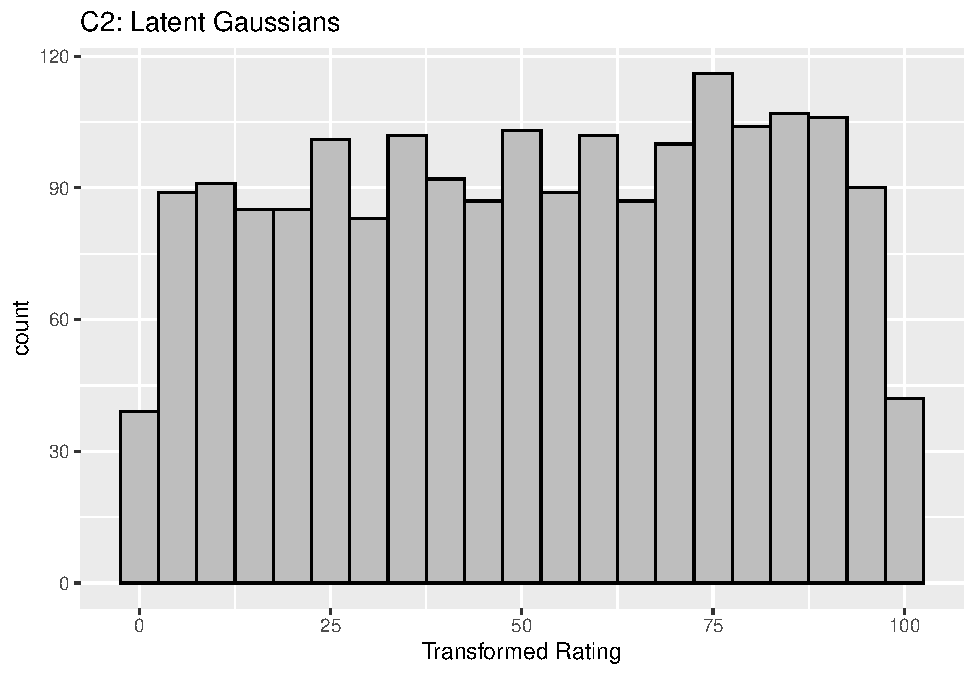
\includegraphics[width=0.33\linewidth]{06-binormal-model_files/figure-latex/unnamed-chunk-4-6} 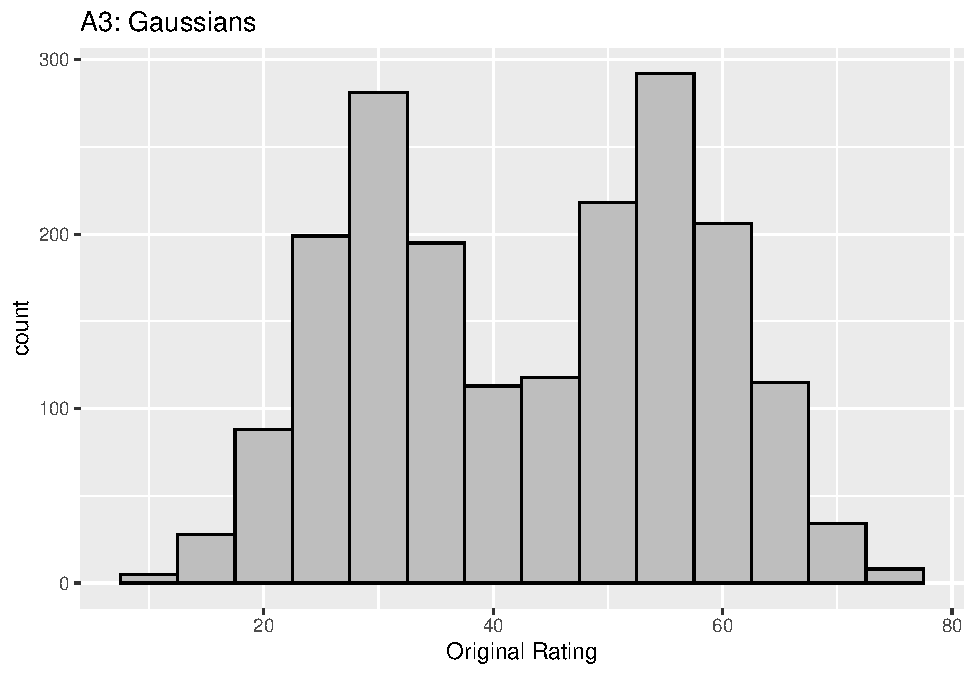
\includegraphics[width=0.33\linewidth]{06-binormal-model_files/figure-latex/unnamed-chunk-4-7} 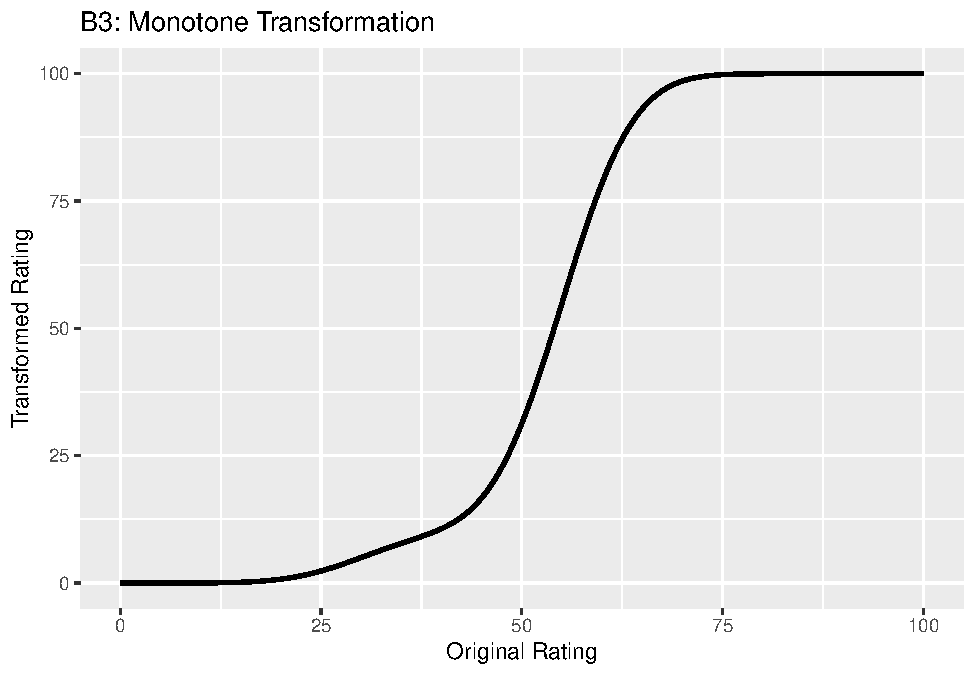
\includegraphics[width=0.33\linewidth]{06-binormal-model_files/figure-latex/unnamed-chunk-4-8} 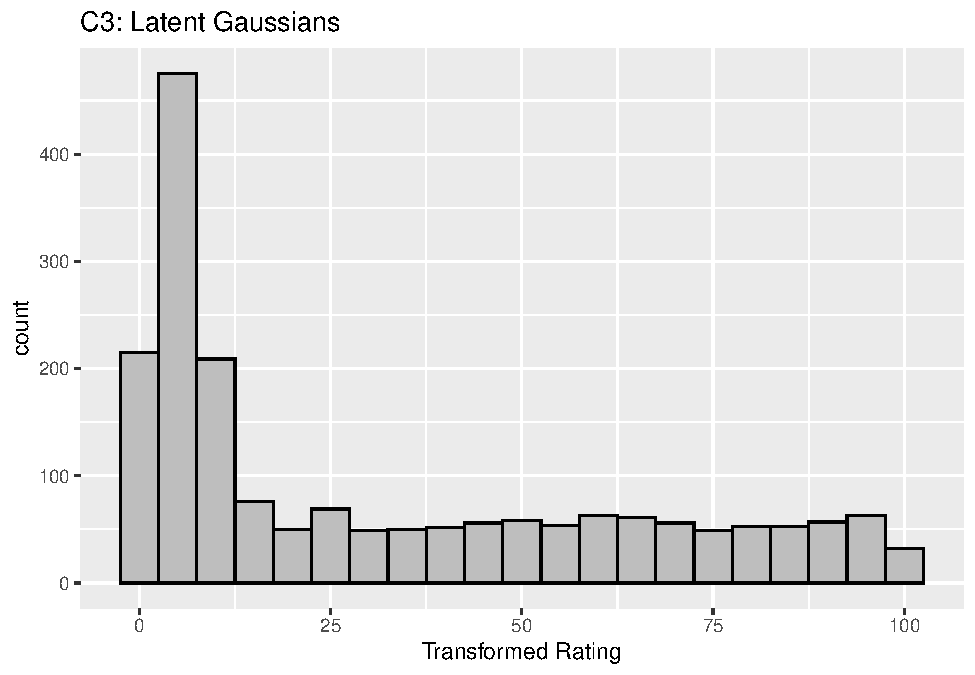
\includegraphics[width=0.33\linewidth]{06-binormal-model_files/figure-latex/unnamed-chunk-4-9}

\textbf{Figure captions (A1 - C3):} Plots illustrating the invariance of ROC analysis to arbitrary monotone transformations of the ratings. Each of the latent Gaussian plots (C1, C2 and C3) appears not binormal. However, by using the inverse of the monotone transformations shown (B1, B2 and B3), they can be transformed to the binormal model histograms (A1, A2 and A3). Plot (A1) shows the histogram of simulated ratings from a binormal model. Two peaks, one at 30 and the other at 55 are evident (by design, all ratings in this figure are in the range 0 to 100). Plot (B1) shows the monotone transformation for \(f = 0.1\). Plot (C1) shows the histogram of the transformed rating. The choice of \(f\) leads to a transformed rating histogram that is peaked near the high end of the rating scale. For (A1) and (C1) the corresponding AUCs are identical (0.99308). Plot (A2) is for a different seed value, plot (B2) is the transformation for \(f = 0.5\) and now the transformed histogram is almost flat, plot C2. For plots (A2) and (C2) the corresponding AUCs are identical (0.9936689). Plot (A3) is for a different seed value, (B3) is the transformation for \(f = 0.9\) and the transformed histogram (C3) is peaked near the low end of the transformed rating scale. For plots (A3) and (C3) the corresponding AUCs are identical (0.9950411).

Line 20-21 sets the parameters of the simulation model. The idea is to simulate continuous ratings data in the range 0 to 100 from a binormal model. Non-diseased cases are sampled from a Gaussian centered at \(\mu_1\) = 30 and standard deviation \(\sigma_1 = 7\). Diseased cases are sampled from a Gaussian centered at \(\mu_2\) = 55 and standard deviation \(\sigma_2\) = 7. The variable \(f\), which is in the range (0,1), controls the shape of the transformed distribution. If \(f\) is small, the transformed distribution will be peaked towards 0 and if \(f\) is unity, it will be peaked at 100. If \(f\) equals 0.5, the transformed distribution is flat. Insight into the reason for this transformation is in \citep{RN300}, Chapter 7, ibid: it has to do with transformations of random variables. The transformation \(Y(Z)\), in the in-line function \(Y\), not shown, implements:

\begin{equation} 
Y\left ( Z \right )=\left [ \left ( 1-f \right )\Phi\left ( \frac{Z-\mu_1}{\sigma_1} \right )+f\Phi\left ( \frac{Z-\mu_2}{\sigma_2} \right ) \right ]100
\label{eq:BinModDemoMisconception}
\end{equation}

The multiplication by 100 ensures that the transformed variable is in the range 0 to 100. The code realizes the random samples, calculates the empirical AUC using the binormal samples, displays the histogram of the binormal samples, plots the transformation function, calculates the empirical AUC using the transformed samples, and plots the histogram of the transformed samples.

The output lists the values of the seed variable and the value of the shape parameter \(f\). \emph{For each value of seed and the shape parameter, the AUCs of the actual Gaussians and the transformed variables are identical to seven digits (set at line 10)}. For this reason, the transformed variables are termed ``Latent Gaussians''. The values of the parameters were chosen to explicate the binormal nature of the plots A2 and A3). This has the effect of making the AUCs close to unity. It is left as an exercise for the reader to plot ROC curves corresponding to actual Gaussian and latent Gaussian variables and show that they are identical.

Fig. (B1) shows the transformation for \(f = 0.1\). The steep initial rise of the curve has the effect of flattening the histogram of the transformed ratings at the low end of the rating scale, Fig. (C1). Conversely, the flat nature of the curve near upper end of the rating range has the effect of causing the histogram of the transformed variable to peak in that range. Fig. (B2) shows the transformation for \(f = 0.5\). This time the transformed rating histogram, Fig. (C2), is almost flat over the entire range. Fig. (B3) shows the transformation for \(f = 0.9\). This time the transformed rating histogram, Fig. (C3) is peaked at the low end of the transformed rating scale.

Each histogram in Fig. (C1, C2 and C3) appears to be non-Gaussian. The corresponding non-diseased and diseased ratings will fail tests of normality. {[}Showing this is left as an exercise for the reader.{]} Nevertheless, the transformed ratings are latent Gaussians in the sense that the inverses of the transformations shown in Fig. (B1, B2 and B3) will yield histograms that are strictly binormal. By appropriate changes to the monotone transformation function, the histograms shown in Fig. (C1, C2 and C3) can be made to resemble a wide variety of shapes. {[}As another exercise, the reader could modify the transformation function to yield quasi-bimodal histograms.{]} \textbf{One concludes that visual examination of the shape of the histogram of ratings yields little, if any, insight into whether the underlying binormal model assumptions are being violated.}

\hypertarget{expressions-for-sensitivity-and-specificity}{%
\subsection{Expressions for sensitivity and specificity}\label{expressions-for-sensitivity-and-specificity}}

Let \(Z_t\) denote the random z-sample for truth state \(t\) (\(t\) = 1 for non-diseased and \(t\) = 2 for diseased cases). Since the distribution of z-samples from disease-free cases is \(N(0,1)\), the expression for specificity, Chapter ``Modeling Binary Paradigm'', Eqn. 3.13, applies. It is reproduced below:

\begin{equation} 
Sp\left ( \zeta \right )=P\left ( Z_1 < \zeta \right )=\Phi\left ( \zeta \right )
\label{eq:BinModSp}
\end{equation}

To obtain an expression for sensitivity, consider that for truth state \(t = 2\), the random variable \(\frac{Z_2-\mu}{\sigma}\) is distributed as \(N(0,1)\):

\begin{equation*} 
\frac{Z_2-\mu}{\sigma}\sim N\left ( 0,1 \right )
\end{equation*}

Sensitivity is \(P\left ( Z_2 > \zeta \right )\), which implies, because \(\sigma\) is positive (subtract from both sides of the ``greater than'' symbol and divide by \(\sigma\)):

\begin{equation} 
Se\left ( \zeta | \mu, \sigma \right )= P\left ( Z_2 > \zeta \right )=P\left ( \frac{Z_2-\mu}{\sigma} > \frac{\zeta-\mu}{\sigma} \right )
\label{eq:BinModSe}
\end{equation}

The right-hand-side can be rewritten as follows:

\begin{equation*} 
Se\left ( \zeta | \mu, \sigma \right )= 1 - P\left ( \frac{Z_2-\mu}{\sigma} \leq  \frac{\zeta-\mu}{\sigma} \right )\\
=1-\Phi\left (  \frac{\zeta-\mu}{\sigma}\right )=\Phi\left (  \frac{\mu-\zeta}{\sigma}\right )
\end{equation*}

Summarizing, the formulae for the specificity and sensitivity for the binormal model are:

\begin{equation} 
Sp\left ( \zeta \right ) = \Phi\left ( \zeta \right )\\
Se\left ( \zeta | \mu, \sigma \right ) = \Phi\left (  \frac{\mu-\zeta}{\sigma}\right )
\label{eq:BinModSeSp}
\end{equation}

The coordinates of the operating point defined by \(\zeta\) are given by:

\begin{equation} 
FPF\left ( \zeta \right ) = 1 - Sp\left ( \zeta \right ) = 1 - \Phi\left ( \zeta \right ) = \Phi\left ( -\zeta \right )
\label{eq:BinModFPF}
\end{equation}

\begin{equation} 
TPF\left ( \zeta | \mu, \sigma \right ) = \Phi\left ( \frac{\mu-\zeta}{\sigma} \right )
\label{eq:BinModTPF}
\end{equation}

These expressions allow calculation of the operating point for any \(\zeta\). An equation for a curve is usually expressed as \(y=f(x)\). An expression of this form for the ROC curve, i.e., the y coordinate (TPF) expressed as a function of the x coordinate (FPF), follows upon inversion of the expression for FPF, Eqn. \eqref{eq:BinModFPF}:

\begin{equation} 
\zeta = -\Phi^{-1}\left ( FPF \right )
\label{eq:BinModZeta}
\end{equation}

Substitution of Eqn. \eqref{eq:BinModZeta} in Eqn. \eqref{eq:BinModTPF} yields:

\begin{equation} 
TPF = \Phi\left ( \frac{\mu + \Phi^{-1}\left (FPF  \right )}{\sigma} \right )
\label{eq:BinModRocCurve1}
\end{equation}

This equation gives the dependence of TPF on FPF, i.e., the equation for the ROC curve. It will be put into standard notation next.

\hypertarget{binormal-model-in-standard-notation}{%
\subsection{Binormal model in standard notation}\label{binormal-model-in-standard-notation}}

The following notation is widely used in the literature:

\begin{equation} 
a=\frac{\mu}{\sigma};b=\frac{1}{\sigma}
\label{eq:BinModabParameters}
\end{equation}

The reason for the \((a,b)\) instead of the \((\mu,\sigma)\) notation is that Dorfman and Alf assumed, in their seminal paper \citep{RN1081}, that the diseased distribution (signal distribution in signal detection theory) had unit variance, and the non-diseased distribution (noise) had standard deviation \(b\) (\(b > 0\)) or variance \(b^2\), and that the separation of the two distributions was \(a\), see figure below. In this example, \(a = 1.11\) and \(b = 0.556\). Dorfman and Alf's fundamental contribution, namely estimating these parameters from ratings data, to be described below, led to the widespread usage of the \((a,b)\) parameters, estimated by their software (RSCORE), and its newer variants (e.g., RSCORE --II, ROCFIT and ROCKIT).

By dividing the z-samples by \(b\), the variance of the distribution labeled ``Noise'' becomes unity, its mean stays at zero, and the variance of the distribution labeled ``Signal'' becomes \(1/b\), and its mean becomes \(a/b\), as shown below. It illustrates that the inverses of Eqn. \eqref{eq:BinModabParameters} are:

\begin{equation} 
\mu=\frac{a}{b};\sigma=\frac{1}{b}
\label{eq:BinModabParametersInv}
\end{equation}

Eqns. \eqref{eq:BinModabParameters} and \eqref{eq:BinModabParametersInv} allow conversion from one notation to another.

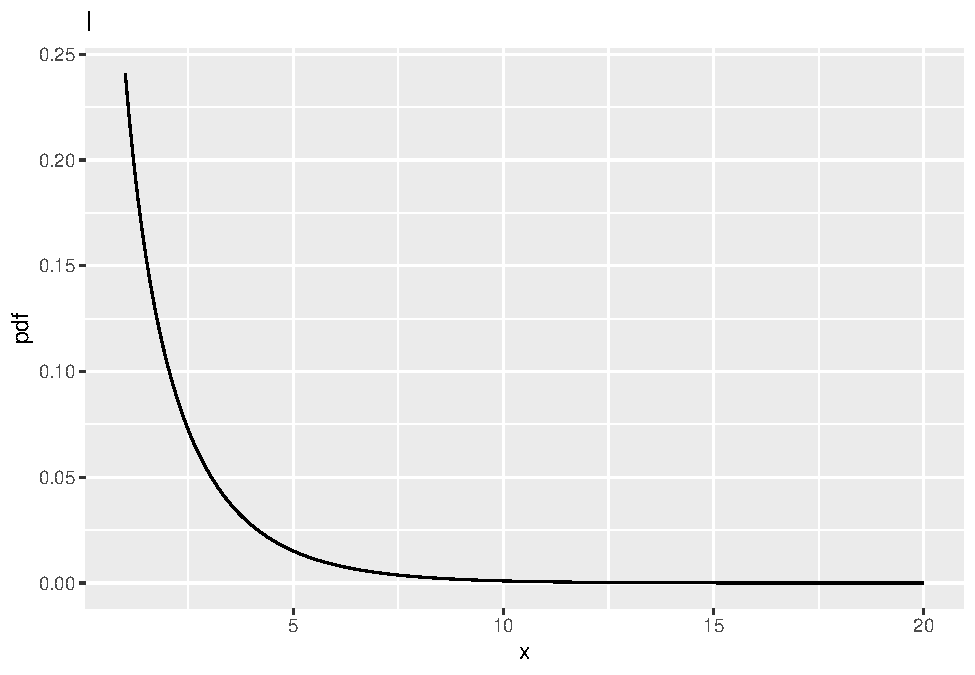
\includegraphics{06-binormal-model_files/figure-latex/unnamed-chunk-5-1.pdf} 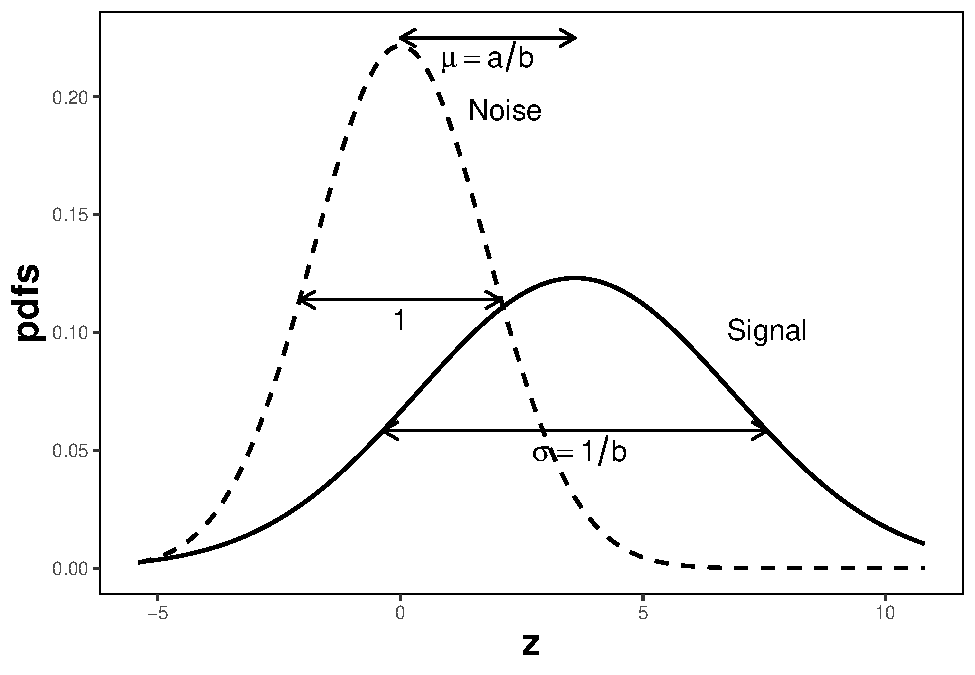
\includegraphics{06-binormal-model_files/figure-latex/unnamed-chunk-5-2.pdf}

\hypertarget{properties-of-the-binormal-model-roc-curve}{%
\subsection{Properties of the binormal model ROC curve}\label{properties-of-the-binormal-model-roc-curve}}

Using the \((a,b)\) notation, Eqn. \eqref{eq:BinModRocCurve1} for the ROC curve reduces to:

\begin{equation} 
TPF = \Phi\left ( a+ b \Phi^{-1}\left (FPF  \right ) \right )
\label{eq:BinModRocCurve}
\end{equation}

Since \(\Phi^{-1}(FPF)\) is an increasing function of its argument \(FPF\), and \(b > 0\), the argument of the \(\Phi\) function is an increasing function of \(FPF\). Since \(\Phi\) is a monotonically increasing function of its argument, \(TPF\) is a monotonically increasing function of \(FPF\). This is true regardless of the sign of \(a\). If \(FPF = 0\), then \(\Phi^{-1}(0) = -\infty\) and \(TPF = 0\). If \(FPF = 1\), then \(\Phi^{-1}(1) = +\infty\) and \(TPF = 1\). {[}The fact that \(TPF\) is a monotonic increasing function of \(FPF\) is consistent with the following argument: to increase \(FPF\), \(\zeta\) must decrease, which increases the area under the diseased distribution to the right of \(\zeta\), i.e., increases \(TPF\).{]}

Regardless of the value of \(a\), as long as \(b \ge 0\), the ROC curve starts at (0,0) and ends at (1,1), increasing monotonically from the origin to (1,1).

From Eqn. \eqref{eq:BinModFPF} and Eqn. \eqref{eq:BinModTPF}, the expressions for \(FPF\) and \(TPF\) in terms of model parameters \((a,b)\) are:

\begin{equation} 
FPF\left ( \zeta \right ) = \Phi\left ( -\zeta \right )\\
\label{eq:BinModFPFab}
\end{equation}

and

\begin{equation} 
TPF = \Phi\left ( a - b \zeta \right )
\label{eq:BinModTPFab}
\end{equation}

\hypertarget{pdfs-of-the-binormal-model}{%
\subsection{pdfs of the binormal model}\label{pdfs-of-the-binormal-model}}

According to Eqn. \eqref{eq:BinModZSampling1} the probability that a z-sample is smaller than a specified threshold \(\zeta\), i.e., the CDF function, is:

\begin{equation*} 
P\left ( Z \le \zeta \mid  Z\sim N\left ( 0,1 \right ) \right ) = 1-FPF\left ( \zeta \right ) = \Phi \left ( \zeta  \right )
\end{equation*}

\begin{equation*} 
P\left ( Z \le \zeta \mid  Z\sim N\left ( \mu,\sigma^2 \right ) \right ) = 1-TPF\left ( \zeta \right ) = \Phi \left ( \frac{\zeta - \mu}{\sigma}  \right )
\end{equation*}

Since the \emph{pdf} is the derivative of the corresponding CDF function, it follows that (the subscripts N and D denote non-diseased and diseased cases, respectively):

\begin{equation*} 
pdf_N\left ( \zeta \right ) = \frac{\partial \Phi\left ( \zeta \right )}{\partial \zeta} = \phi\left ( \zeta \right ) \equiv \frac{1}{\sqrt{2 \pi}}\exp\left ( -\frac{\zeta^2}{2} \right )
\end{equation*}

\begin{equation*} 
pdf_D\left ( \zeta \right ) = \frac{\partial \Phi\left ( \frac{\zeta - \mu}{\sigma} \right )}{\partial \zeta} = \frac{1}{\sigma} \phi\left ( \frac{\zeta - \mu}{\sigma} \right ) \equiv \frac{1}{\sqrt{2 \pi}\sigma}\exp\left ( -\frac{\left (\zeta-\mu  \right )^2}{2\sigma} \right )
\end{equation*}

The second equation can be written in \((a,b)\) notation as:

\begin{equation*} 
pdf_D\left ( \zeta \right ) = b\phi\left ( b\zeta-a \right ) = \frac{b}{\sqrt{2 \pi}}\exp\left ( -\frac{\left (b\zeta - a \right )^2}{2} \right )
\end{equation*}

Generation of pdfs for specified values of binormal model parameters was illustrated above (ref. TBA to previous chapter?) for specified values of \(\mu,\sigma\). Using transformations in Eqn. \eqref{eq:BinModabParameters} the code can be readily converted to accept \((a,b)\) values as inputs.

\hypertarget{fitting-the-roc-curve}{%
\subsection{Fitting the ROC curve}\label{fitting-the-roc-curve}}

To be described next is a method for fitting data such as in Table \ref{tab:ratingsParadigmTable1} to the binormal model, i.e., determining the parameters \(a,b\) and the thresholds \(\zeta_r , r = 1, 2, ..., R-1\), to best fit, in some to-be-defined sense, the observed cell counts. The most common method uses an algorithm called maximum likelihood. But before getting to that, I describe the least-square method, which is conceptually simpler, but not really applicable to this type of fitting.

\hypertarget{least-squares-estimation}{%
\subsection{Least-squares estimation}\label{least-squares-estimation}}

By applying the function \(\Phi^{-1}\) to both sides of Eqn. (6.2.17), one gets (the ``inverse'' function cancels the ``forward'' function on the right hand side):

\begin{equation*} 
\Phi^{-1}\left ( TPF \right ) = a + b \Phi^{-1}\left ( FPF \right )
\end{equation*}

This suggests that a plot of \(y = \Phi^{-1}\left ( TPF \right )\) vs.~\(\Phi^{-1}\left ( FPF \right )\) is expected to follow a straight line with slope b and intercept a. Fitting a straight line to such data is generally performed by the method of least-squares, a capability present in most software packages and even spreadsheets, e.g., Excel. Alternatively one can simply visually draw the best straight line that fits the points, memorably referred to7 as ``chi-by-eye''. This was the way parameters of the binormal model were estimated prior to Dorfman and Alf's work3. The least-squares method is a quantitative way of accomplishing the same aim. If \(\left ( x_t,y_t \right )\) are the data points, one constructs \(S\), the sum of the squared deviations of the observed ordinates from the predicted values:

\begin{equation*} 
S  = \sum_{i=1}^{R-1}\left ( y_i - \left ( a + bx_i \right ) \right )^2
\end{equation*}

The idea is to minimize S with respect to the parameters \((a,b)\). One approach is to differentiate this with respect to \(a\) and \(b\) and equate each resulting derivate expression to zero. This yields two equations in two unknowns, which are solved for \(a\) and \(b\). If the reader has never done this before, one should go through these steps at least once, but it would be smarter in future to use software that does all this. In \texttt{R} the least-squares fitting function is \texttt{lm(y\textasciitilde{}x)}, which in its simplest form fits a linear model using the method of least-squares (in case you are wondering lm stands for linear model, a whole branch of statistics in itself; in this example one is using its simplest capability).

\begin{Shaded}
\begin{Highlighting}[]
\CommentTok{\# ML estimates of a and b (from Eng JAVA program)}
\CommentTok{\# a \textless{}{-} 1.3204; b \textless{}{-} 0.6075 }
\CommentTok{\# \# these are not used in program; just there for comparison}

\NormalTok{FPF \textless{}{-}}\StringTok{ }\KeywordTok{c}\NormalTok{(}\FloatTok{0.017}\NormalTok{, }\FloatTok{0.050}\NormalTok{, }\FloatTok{0.183}\NormalTok{, }\FloatTok{0.5}\NormalTok{)  }
\CommentTok{\# this is from Table 6.11, last two rows}
\NormalTok{TPF \textless{}{-}}\StringTok{ }\KeywordTok{c}\NormalTok{(}\FloatTok{0.440}\NormalTok{, }\FloatTok{0.680}\NormalTok{, }\FloatTok{0.780}\NormalTok{, }\FloatTok{0.900}\NormalTok{)}
\CommentTok{\# ...do...}

\NormalTok{PhiInvFPF \textless{}{-}}\StringTok{ }\KeywordTok{qnorm}\NormalTok{(FPF)}
\CommentTok{\# apply the PHI\_INV function}
\NormalTok{PhiInvTPF \textless{}{-}}\StringTok{ }\KeywordTok{qnorm}\NormalTok{(TPF)}
\CommentTok{\# ... do ... }

\NormalTok{fit \textless{}{-}}\StringTok{ }\KeywordTok{lm}\NormalTok{(PhiInvTPF}\OperatorTok{\textasciitilde{}}\NormalTok{PhiInvFPF)}
\KeywordTok{print}\NormalTok{(fit)}
\CommentTok{\#\textgreater{} }
\CommentTok{\#\textgreater{} Call:}
\CommentTok{\#\textgreater{} lm(formula = PhiInvTPF \textasciitilde{} PhiInvFPF)}
\CommentTok{\#\textgreater{} }
\CommentTok{\#\textgreater{} Coefficients:}
\CommentTok{\#\textgreater{} (Intercept)    PhiInvFPF  }
\CommentTok{\#\textgreater{}      1.3288       0.6307}
\NormalTok{pointsData \textless{}{-}}\StringTok{ }\KeywordTok{data.frame}\NormalTok{(}\DataTypeTok{PhiInvFPF =}\NormalTok{ PhiInvFPF, }
                         \DataTypeTok{PhiInvTPF =}\NormalTok{ PhiInvTPF)}
\NormalTok{pointsPlot \textless{}{-}}\StringTok{ }\KeywordTok{ggplot}\NormalTok{(}\DataTypeTok{data =}\NormalTok{ pointsData, }
                     \DataTypeTok{mapping =} 
                       \KeywordTok{aes}\NormalTok{(}\DataTypeTok{x =}\NormalTok{ PhiInvFPF, }
                           \DataTypeTok{y =}\NormalTok{ PhiInvTPF)) }\OperatorTok{+}\StringTok{ }
\StringTok{  }\KeywordTok{geom\_point}\NormalTok{(}\DataTypeTok{size =} \DecValTok{2}\NormalTok{) }\OperatorTok{+}\StringTok{ }
\StringTok{  }\KeywordTok{theme}\NormalTok{(}
    \DataTypeTok{axis.title.y =} \KeywordTok{element\_text}\NormalTok{(}\DataTypeTok{size =} \DecValTok{18}\NormalTok{,}\DataTypeTok{face=}\StringTok{"bold"}\NormalTok{),}
    \DataTypeTok{axis.title.x =} \KeywordTok{element\_text}\NormalTok{(}\DataTypeTok{size =} \DecValTok{18}\NormalTok{,}\DataTypeTok{face=}\StringTok{"bold"}\NormalTok{)) }\OperatorTok{+}
\StringTok{  }\KeywordTok{geom\_abline}\NormalTok{(}
    \DataTypeTok{slope =}\NormalTok{ fit}\OperatorTok{$}\NormalTok{coefficients[}\DecValTok{2}\NormalTok{], }
    \DataTypeTok{intercept =}\NormalTok{ fit}\OperatorTok{$}\NormalTok{coefficients[}\DecValTok{1}\NormalTok{], }\DataTypeTok{size =} \FloatTok{0.75}\NormalTok{)}
\KeywordTok{print}\NormalTok{(pointsPlot)}
\end{Highlighting}
\end{Shaded}

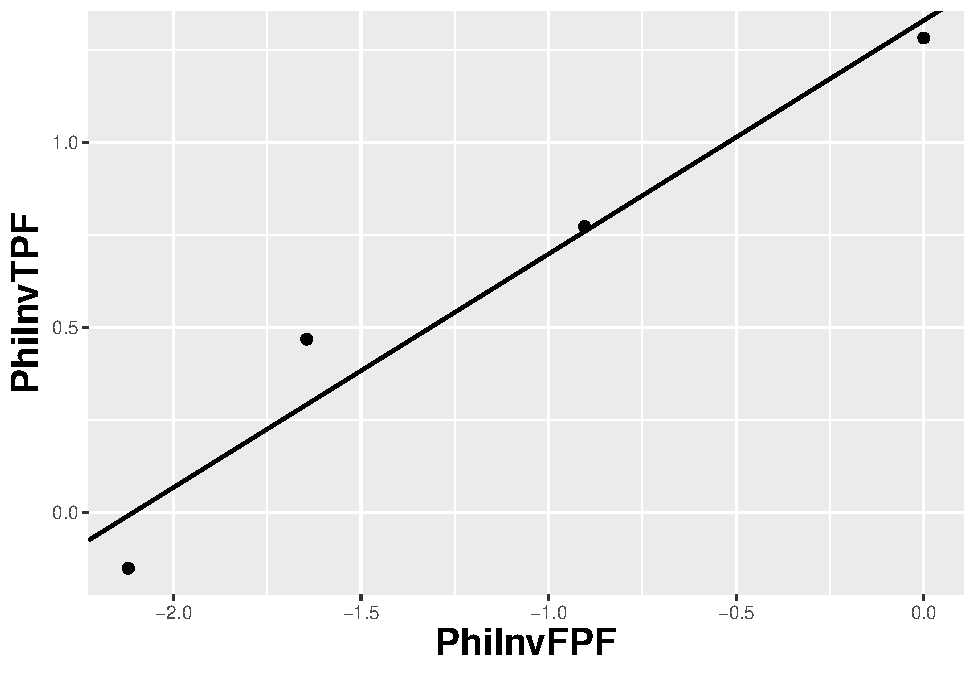
\includegraphics{06-binormal-model_files/figure-latex/unnamed-chunk-6-1.pdf}

This plot shows operating points from Table 1, transformed by the \(\Phi^{-1}\) function; the slope of the line is the least-squares estimate of the \(b\) parameter and the intercept is the corresponding \(a\) parameter of the binormal model.

The first two lines of the output are simply a reminder about the names of the dependent and independent variables. The last line contains the least squares estimated values, \(a\) = 1.3288 and \(b\) = 0.6307. The corresponding maximum likelihood estimates of these parameters, as yielded by the Eng web code, Appendix B, are listed in line 4 of the main program: \(a\) = 1.3204 and \(b\) = 0.6075. The estimates appear to be close, particularly the estimate of \(a\) , but there are a few things wrong with the least-squares approach. First, the method of least squares assumes that the data points are independent. Because of the manner in which they are constructed, namely by cumulating points, the independence assumption is not valid for ROC operating points. Cumulating the 4 and 5 responses constrains the resulting operating point to be above and to the right of the point obtained by cumulating the 5 responses only, so the data points are definitely not independent. Similarly, cumulating the 3, 4 and 5 responses constrains the resulting operating point to be above and to the right of the point obtained by cumulating the 4 and 5 responses, and so on. The second problem is the linear least-squares method assumes there is no error in measuring x; the only source of error that is accounted for is in the y-coordinate. In fact, both coordinates of an ROC operating point are subject to sampling error. Third, disregard of error in the x-direction is further implicit in the estimates of the thresholds, which according to Eqn. (6.2.19), is given by:

\begin{equation*} 
\zeta_r = - \Phi^{-1}\left ( FPF_r \right )
\end{equation*}

These are ``rigid'' estimates that assume no error in the FPF values. As was shown in Chapter \ref{binaryTask}, 95\% confidence intervals apply to these estimates.

{[}A historical note: prior to computers and easy access to statistical functions the analyst had to use a special plotting paper, termed ``double probability paper'', that converted probabilities into x and y distances using the inverse function. The complement of the inverse function is sometimes termed the z-deviate.4 Since this term confused me when I entered this field ca. 1985, and it confuses me even now, I will not use it further.{]}

\hypertarget{maximum-likelihood-estimation-mle}{%
\section{Maximum likelihood estimation (MLE)}\label{maximum-likelihood-estimation-mle}}

The approach taken by Dorfman and Alf was to maximize the likelihood function instead of S. The likelihood function is the probability of the observed data given a set of parameter values, i.e.,

\begin{equation*} 
\text {L} \equiv P\left ( data \mid \text {parameters} \right )
\end{equation*}

Generally ``data'' is suppressed, so likelihood is a function of the parameters; but ``data'' is always implicit. With reference to Fig. 6.1, the probability of a non-diseased case yielding a count in the 2nd bin equals the area under the curve labeled ``Noise'' bounded by the vertical lines at \(\zeta_1\) and \(\zeta_2\). In general, the probability of a non-diseased case yielding a count in the \(r^\text{th}\) bin equals the area under the curve labeled ``Noise'' bounded by the vertical lines at \(\zeta_{r-1}\) and \(\zeta_r\). Since the area to the left of a threshold is the CDF corresponding to that threshold, the required probability is \(\Phi\left ( \zeta_r \right ) - \Phi\left ( \zeta_{r-1} \right )\); we are simply subtracting two expressions for specificity, Eqn. (6.2.5).

\begin{equation*} 
\text {count in non-diseased bin } r = \Phi\left ( \zeta_r \right ) - \Phi\left ( \zeta_{r-1} \right )
\end{equation*}

Similarly, the probability of a diseased case yielding a count in the rth bin equals the area under the curve labeled ``Signal'' bounded by the vertical lines at \(\zeta_{r-1}\) and \(\zeta_r\). The area under the diseased distribution to the left of threshold \(\zeta_r\) is the \(1 - TPF\) at that threshold:

\begin{equation*} 
1 - \Phi\left ( \frac{\mu-\zeta_r}{\sigma} \right ) = \Phi\left ( \frac{\zeta_r - \mu}{\sigma} \right )
\end{equation*}

The area between the two thresholds is:

\begin{align*} 
P\left ( \text{count in diseased bin }r \right ) &= \Phi\left ( \frac{\zeta_r - \mu}{\sigma} \right ) - \Phi\left ( \frac{\zeta_{r-1} - \mu}{\sigma} \right ) \\
&= \Phi\left ( b\zeta_r-a \right ) - \Phi\left ( b\zeta_{r-1}-a \right )
\end{align*}

Let \(K_{1r}\) denote the number of non-diseased cases in the rth bin, and \(K_{2r}\) denotes the number of diseased cases in the rth bin. Consider the number of counts \(K_{1r}\) in non-diseased case bin \(r\). Since the probability of each count is \(\Phi\left ( \zeta_{r+1} \right ) - \Phi\left ( \zeta_r \right )\), the probability of the observed number of counts, assuming the counts are independent, is \({\left(\Phi\left ( \zeta_{r+1} \right ) - \Phi\left ( \zeta_r \right ) \right )}^{K_{1r}}\). Similarly, the probability of observing counts in diseased case bin \(r\) is \({\left (\Phi\left ( b\zeta_{r+1}-a \right ) - \Phi\left ( b\zeta_r-a \right ) \right )}^{K_{2r}}\), subject to the same independence assumption. The probability of simultaneously observing \(K_{1r}\) counts in non-diseased case bin r and \(K_{2r}\) counts in diseased case bin \(r\) is the product of these individual probabilities (again, an independence assumption is being used):

\begin{equation*} 
\left (\Phi\left ( \zeta_{r+1}  \right ) - \Phi\left ( \zeta_r  \right )  \right )^{K_{1r}} \left (\Phi\left ( b\zeta_{r+1}-a  \right ) - \Phi\left ( b\zeta_r-a  \right )  \right )^{K_{2r}}
\end{equation*}

Similar expressions apply for all integer values of \(r\) ranging from \(1,2,...,R\). Therefore the probability of observing the entire data set is the product of expressions like Eqn. (6.4.5), over all values of \(r\):

\begin{equation} 
\prod_{r=1}^{R}\left [\left (\Phi\left ( \zeta_{r+1}  \right ) - \Phi\left ( \zeta_r  \right )  \right )^{K_{1r}} \left (\Phi\left ( b\zeta_{r+1}-a  \right ) - \Phi\left ( b\zeta_r-a  \right )  \right )^{K_{2r}}  \right ]
\label{eq:BinModProductProb}
\end{equation}

We are almost there. A specific combination of \(K_{11},K_{12},...,K_{1R}\) counts from \(K_1\) non-diseased cases and counts \(K_{21},K_{22},...,K_{2R}\) from \(K_2\) diseased cases can occur the following number of times (given by the multinomial factor shown below):

\begin{equation} 
\frac{K_1!}{\prod_{r=1}^{R}K_{1r}!}\frac{K_2!}{\prod_{r=1}^{R}K_{2r}!}
\label{eq:BinModCombFactor}
\end{equation}

The likelihood function is the product of Eqn. \eqref{eq:BinModProductProb} and Eqn. \eqref{eq:BinModCombFactor}:

\begin{equation} 
\begin{split}
L\left ( a,b,\overrightarrow{\zeta} \right ) &= \left (\frac{K_1!}{\prod_{r=1}^{R}K_{1r}!}\frac{K_2!}{\prod_{r=1}^{R}K_{2r}!}  \right ) \times \\
&\quad\prod_{r=1}^{R}\left [\left (\Phi\left ( \zeta_{r+1}  \right ) - \Phi\left ( \zeta_r  \right )  \right )^{K_{1r}} \left (\Phi\left ( b\zeta_{r+1}-a  \right ) - \Phi\left ( b\zeta_r-a  \right )  \right )^{K_{2r}}  \right ]
\end{split}
\label{eq:BinModLikelihood}
\end{equation}

The left hand side of Eqn. \eqref{eq:BinModLikelihood} shows explicitly the dependence of the likelihood function on the parameters of the model, namely \(a,b,\overrightarrow{\zeta}\), where the vector of thresholds \(\overrightarrow{\zeta}\) is a compact notation for the set of thresholds \(\zeta_1,\zeta_2,...,\zeta_R\), (note that since \(\zeta_0 = -\infty\), and \(\zeta_R = +\infty\), only \(R-1\) free threshold parameters are involved, and the total number of free parameters in the model is \(R+1\)). For example, for a 5-rating ROC study, the total number of free parameters is 6, i.e., \(a\), \(b\) and 4 thresholds \(\zeta_1,\zeta_2,\zeta_3,\zeta_4\).

Eqn. \eqref{eq:BinModLikelihood} is forbidding but here comes a simplification. The difference of probabilities such as \(\Phi\left ( \zeta_r \right )-\Phi\left ( \zeta_{r-1} \right )\) is guaranteed to be positive and less than one {[}the \(\Phi\) function is a probability, i.e., in the range 0 to 1, and since \(\zeta_r\) is greater than \(\zeta_{r-1}\), the difference is positive and less than one{]}. When the difference is raised to the power of \(K_{1r}\) (a non-negative integer) a very small number can result. Multiplication of all these small numbers may result in an even smaller number, which may be too small to be represented as a floating-point value, especially as the number of counts increases. To prevent this we resort to a trick. Instead of maximizing the likelihood function \(L\left ( a,b,\overrightarrow{\zeta} \right )\) we choose to maximize the logarithm of the likelihood function (the base of the logarithm is immaterial). The logarithm of the likelihood function is:

\begin{equation} 
LL\left ( a,b,\overrightarrow{\zeta} \right )=\log \left ( L\left ( a,b,\overrightarrow{\zeta} \right ) \right )
\label{eq:BinModLogLikelihood}
\end{equation}

Since the logarithm is a monotonically increasing function of its argument, maximizing the logarithm of the likelihood function is equivalent to maximizing the likelihood function. Taking the logarithm converts the product symbols in Eqn. (6.4.8) to summations, so instead of multiplying small numbers one is adding them, thereby avoiding underflow errors. Another simplification is that one can ignore the logarithm of the multinomial factor involving the factorials, because these do not depend on the parameters of the model. Putting all this together, we get the following expression for the logarithm of the likelihood function:

\begin{equation} 
\begin{split}
LL\left ( a,b,\overrightarrow{\zeta} \right ) \propto& \sum_{r=1}^{R} K_{1r}\log \left ( \Phi\left ( \zeta_{r+1} \right ) - \Phi\left ( \zeta_r \right ) \right ) \\
&+ \sum_{r=1}^{R} K_{2r}\log \left ( \Phi\left (b \zeta_{r+1} - a \right ) - \Phi\left ( b \zeta_r - a \right ) \right ) 
\end{split}
\label{eq:BinModLL}
\end{equation}

The left hand side of Eqn. \eqref{eq:BinModLL} is a function of the model parameters \(a,b,\overrightarrow{\zeta}\) and the observed data, the latter being the counts contained in the vectors \(\overrightarrow{K_1}\) and \(\overrightarrow{K_2}\), where the vector notation is used as a compact form for the counts \(K_{11},K_{12},...,K_{1R}\) and \(K_{21},K_{22},...,K_{2R}\), respectively. The right hand side of Eqn. \eqref{eq:BinModLL} is monotonically related to the probability of observing the data given the model parameters \(a,b,\overrightarrow{\zeta}\). If the choice of model parameters is poor, then the probability of observing the data will be small and log likelihood will be small. With a better choice of model parameters the probability and log likelihood will increase. With optimal choice of model parameters the probability and log likelihood will be maximized, and the corresponding optimal values of the model parameters are called maximum likelihood estimates (MLEs). These are the estimates produced by the programs RSCORE and ROCFIT.

\hypertarget{code-implementing-mle}{%
\subsection{Code implementing MLE}\label{code-implementing-mle}}

\begin{Shaded}
\begin{Highlighting}[]

\CommentTok{\# ML estimates of a and b (from Eng JAVA program)}
\CommentTok{\# a \textless{}{-} 1.3204; b \textless{}{-} 0.6075 }
\CommentTok{\# these are not used in program; just there for comparison}

\NormalTok{K1t \textless{}{-}}\StringTok{ }\KeywordTok{c}\NormalTok{(}\DecValTok{30}\NormalTok{, }\DecValTok{19}\NormalTok{, }\DecValTok{8}\NormalTok{, }\DecValTok{2}\NormalTok{, }\DecValTok{1}\NormalTok{)}
\NormalTok{K2t \textless{}{-}}\StringTok{ }\KeywordTok{c}\NormalTok{(}\DecValTok{5}\NormalTok{,  }\DecValTok{6}\NormalTok{, }\DecValTok{5}\NormalTok{, }\DecValTok{12}\NormalTok{, }\DecValTok{22}\NormalTok{)}
\NormalTok{dataset \textless{}{-}}\StringTok{ }\KeywordTok{Df2RJafrocDataset}\NormalTok{(K1t, K2t, }\DataTypeTok{InputIsCountsTable =} \OtherTok{TRUE}\NormalTok{)}
\NormalTok{retFit \textless{}{-}}\StringTok{ }\KeywordTok{FitBinormalRoc}\NormalTok{(dataset)}
\NormalTok{retFit[}\DecValTok{1}\OperatorTok{:}\DecValTok{5}\NormalTok{]}
\CommentTok{\#\textgreater{} $a}
\CommentTok{\#\textgreater{} [1] 1.320453}
\CommentTok{\#\textgreater{} }
\CommentTok{\#\textgreater{} $b}
\CommentTok{\#\textgreater{} [1] 0.6074929}
\CommentTok{\#\textgreater{} }
\CommentTok{\#\textgreater{} $zetas}
\CommentTok{\#\textgreater{}    zetaFwd1    zetaFwd2    zetaFwd3    zetaFwd4 }
\CommentTok{\#\textgreater{} 0.007680547 0.896273068 1.515647850 2.396722099 }
\CommentTok{\#\textgreater{} }
\CommentTok{\#\textgreater{} $AUC}
\CommentTok{\#\textgreater{} [1] 0.8704522}
\CommentTok{\#\textgreater{} }
\CommentTok{\#\textgreater{} $StdAUC}
\CommentTok{\#\textgreater{}            [,1]}
\CommentTok{\#\textgreater{} [1,] 0.03790423}
\KeywordTok{print}\NormalTok{(retFit}\OperatorTok{$}\NormalTok{fittedPlot)}
\end{Highlighting}
\end{Shaded}

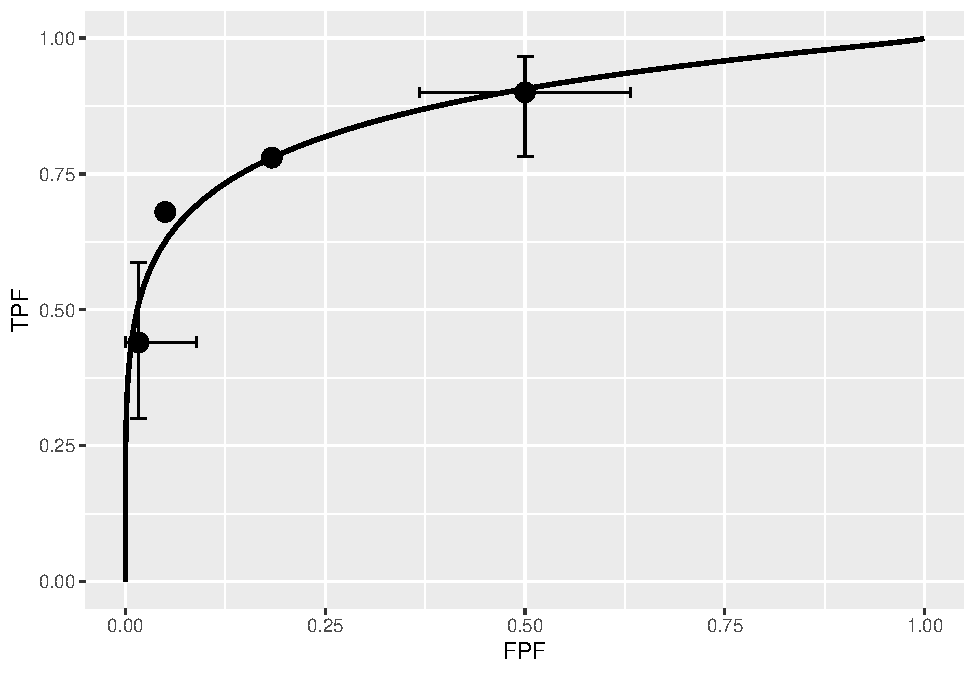
\includegraphics{06-binormal-model_files/figure-latex/unnamed-chunk-7-1.pdf}

Note the usage of the \texttt{RJafroc} package \citep{R-RJafroc}. Specifically, the function \texttt{FitBinormalRoc}. The ratings table is converted to an \texttt{RJafroc} dataset object, followed by application of the fitting function. The results, contained in \texttt{retFit} should be compared to those obtained from the \href{http://www.rad.jhmi.edu/jeng/javarad/roc/JROCFITi.html}{website implementation of ROCFIT}.

\hypertarget{validating-the-fitting-model}{%
\subsection{Validating the fitting model}\label{validating-the-fitting-model}}

The above ROC curve is a good visual fit to the observed operating points. Quantification of the validity of the fitting model is accomplished by calculating the Pearson goodness-of-fit test \citep{RN2656}, also known as the chi-square test, which uses the statistic defined by \citep{RN1492}:

\begin{equation} 
C^2=\sum_{t=1}^{2}\sum_{r=1}^{R}\frac{\left (K_{tr}-\left \langle K_{tr} \right \rangle  \right )^2}{\left \langle K_{tr} \right \rangle}\\
K_{tr} \geq 5
\label{eq:BinModGoodnessFit}
\end{equation}

The expected values are given by:

\begin{equation}
\begin{split}
\left \langle K_{1r} \right \rangle &=K_1\left ( \Phi\left ( \zeta_{r+1} \right ) - \Phi\left ( \zeta_r \right )  \right ) \\
\left \langle K_{2r} \right \rangle &=K_2\left ( \Phi\left ( a\zeta_{r+1}-b \right ) - \Phi\left ( a\zeta_r - b\right )  \right )
\end{split}
\label{eq:BinModGoodnessFitExpVals}
\end{equation}

These expressions should make sense: the difference between the two CDF functions is the probability of a count in the specified bin, and multiplication by the total number of relevant cases should yield the expected counts (a non-integer).

It can be shown that under the null hypothesis that the assumed probability distribution functions for the counts equals the true probability distributions, i.e., the model is valid, the statistic \(C^2\) is distributed as:

\begin{equation} 
C^2\sim \chi_{df}^{2}
\label{eq:BinModGoodnessFitDistr}
\end{equation}

Here \(C^2\sim \chi_{df}^{2}\) is the chi-square distribution with degrees of freedom \emph{df} defined by:

\begin{equation} 
df=\left ( R-1 \right )+\left ( R-1 \right )-\left (2+ R-1 \right )=\left ( R-3 \right )
\label{eq:BinModGoodnessFitdf}
\end{equation}

The right hand side of the above equation has been written in an expansive form to illustrate the general rule: for \(R\) non-diseased cells in the ratings table, the degree of freedom is \(R-1\): this is because when all but one cells are specified, the last is determined, because they must sum to \(K_1\) . Similarly, the degree of freedom for the diseased cells is also \(R-1\). Last, we need to subtract the number of free parameters in the model, which is \((2+R-1)\), i.e., the \(a,b\) parameters and the \(R-1\) thresholds. It is evident that if \(R = 3\) then \(df = 0\). In this situation, there are only two non-trivial operating points and the straight-line fit shown will pass through both of them. With two basic parameters, fitting two points is trivial, and goodness of fit cannot be calculated.

Under the null hypothesis (i.e., model is valid) \(C^2\) is distributed as \(\chi_{df}^{2}\). Therefore, one computes the probability that this statistic is larger than the observed value, called the \emph{p-value}. If this probability is very small, that means that the deviations of the observed values of the cell counts from the expected values are so large that it is unlikely that the model is correct. The degree of unlikeliness is quantified by the p-value. Poor fits lead to small p values.

At the 5\% significance level, one concludes that the fit is not good if \(p < 0.05\). In practice one occasionally accepts smaller values of \(p\), \(p > 0.001\) before completely abandoning a model. It is known that adoption of a stricter criterion, e.g., \(p > 0.05\), can occasionally lead to rejection of a retrospectively valid model \citep{RN300}.

\hypertarget{estimating-the-covariance-matrix}{%
\subsection{Estimating the covariance matrix}\label{estimating-the-covariance-matrix}}

TBA See book chapter 6.4.3. This is implemented in RJafroc.

\hypertarget{estimating-the-variance-of-az}{%
\subsection{Estimating the variance of Az}\label{estimating-the-variance-of-az}}

TBA See book chapter 6.4.4. This is implemented in RJafroc.

\hypertarget{single-fom-derived-from-roc-curve}{%
\subsection{Single FOM derived from ROC curve}\label{single-fom-derived-from-roc-curve}}

Sensitivity and specificity are \emph{dual} measures of overall performance. It is hard to unambiguosly compare two systems usng dual measures. What if sensitivity is higher for one system but specificity is higher for another. This is, of course, a consequence of sensitivity/specificity depending on the position of the operating point on the ROC curve. Desirable is a \emph{single} measure of performance that takes into account performance over the entire ROC curve. Two commonly used measures are the binormla model predicted area \(A_z\) under the ROC curve, and the \(d'\) index.

(Book) Appendix 6.A derives the formula for the partial area under the unequal-variance binormal model. A special case of this formula is the area under the whole ROC curve, reproduced below using both parameterizations of the model:

\begin{equation} 
A_z=\Phi\left ( \frac{a}{\sqrt{1+b^2}} \right )=\Phi\left ( \frac{\mu}{\sqrt{1+\sigma^2}} \right )
\label{eq:BinModab2Az}
\end{equation}

The binormal fitted AUC increases as \(a\) increases or as \(b\) decreases. Equivalently, it increases as \(\mu\) increases or as \(\sigma\) decreases. An equivalent \(d'\) parameter is defined as the separation of two unit-variance normal distributions yielding the same AUC as that predicted by the \((a,b)\) parameter binormal model. It is defined by:

\begin{equation} 
d'=\sqrt{2}\Phi^{-1}\left ( A_z \right )
\label{eq:BinModab2dprime}
\end{equation}

\hypertarget{discussion}{%
\section{Discussion}\label{discussion}}

The binormal model is historically very important and the contribution by Dorfman and Alf \citep{RN212} was seminal. Prior to their work, there was no valid way of estimating AUC from observed ratings counts. Their work and a key paper by Lusted \citep{RN1487} accelerated research using ROC methods. The number of publications using their algorithm, and the more modern versions developed by Metz and colleagues, is probably well in excess of 500. Because of its key role, the author has endeavored to take out some of the mystery about how the binormal model parameters are estimated. In particular, a common misunderstanding that the binormal model assumptions are violated by real datasets, when in fact it is quite robust to apparent deviations from normality, is addressed.

A good understanding of this chapter should enable the reader to better understand alternative ROC models, discussed later.

It has been stated that the \texttt{b}-parameter of the binormal model is generally observed to be less than one, consistent with the diseased distribution being wider than the non-diseased one. The ROC literature is largely silent on the reason for this finding. One reason, namely location uncertainty, is presented in Chapter ``Predictions of the RSM'', where RSM stands for Radiological Search Model. Basically, if the location of the lesion is unknown, then z-samples from diseased cases can be of two types, samples from the correct lesion location, or samples from other non-lesion locations. The resulting mixture distribution will then appear to have larger variance than the corresponding samples from non-diseased cases. This type of mixing need not be restricted to location uncertainty. Even is location is known, if the lesions are non-homogenous (e.g., they contain a range of contrasts) then a similar mixture-distribution induced broadening is expected. The contaminated binormal model (CBM) - see Chapter TBA - also predicts that the diseased distribution is wider than the non-diseased one.

The fact that the \texttt{b}-parameter is less than unity implies that the predicted ROC curve is improper, meaning its slope is not monotone decreasing as the operating point moves up the curve. The result is that a portion of the curve, near (1,1) that crosses the chance-diagonal and hooks upward approaching (1,1) with infinite slope. Ways of fitting proper ROC curves are described in Chapter ``Other proper ROC models''. Usually the hook is not readily visible, which has been used as an excuse to ignore the problem. For example, in Fig. 6.4, one would have to ``zoom-in'' on the upper right corner to see it, but the reader should make no mistake about it, the hook is there as .

A recent example is Fig. 1 in the publication resulting from the Digital Mammographic Imaging Screening Trial (DMIST) clinical trial \citep{RN1784} involving 49,528 asymptomatic women from 33 clinical sites and involving 153 radiologists, where each of the film modality ROC plots crosses the chance diagonal and hooks upwards to (1,1), which as is known, results anytime .

The unphysical nature of the hook (predicting worse than chance-level performance for supposedly expert readers) is not the only reason for seeking alternate ROC models. The binormal model is susceptible to degeneracy problems. If the dataset does not provide any interior operating points (i.e., all observed points lie on the axes defined by FPF = 0 or TPF = 1) then the model fits these points with b = 0. The resulting straight-line segment fits do not make physical sense. These problems are addressed by the contaminated binormal model16 to be discussed in Chapter ``Other proper ROC models''. The first paper in the series has particularly readable accounts of data degeneracy.

To this day the binormal model is widely used to fit ROC datasets. In spite of its limitations, the binormal model has been very useful in bringing a level of quantification to this field that did not exist prior to the work \citep{RN212} by Dorfman and Alf.

\hypertarget{BinMod-Summary}{%
\section{Summary}\label{BinMod-Summary}}

\hypertarget{BinMod-Discussion}{%
\section{Discussion}\label{BinMod-Discussion}}

\hypertarget{BinMod-references}{%
\section{References}\label{BinMod-references}}

\hypertarget{HypothesisTesting}{%
\chapter{Hypothesis Testing}\label{HypothesisTesting}}

\hypertarget{HypothesisTesting-introduction}{%
\section{Introduction}\label{HypothesisTesting-introduction}}

The problem addressed here is how to decide whether an estimate of AUC is consistent with a pre-specified value. One example of this is when a single-reader rates a set of cases in a single-modality, from which one estimates AUC, and the question is whether the estimate is statistically consistent with a pre-specified value. From a clinical point of view, this is generally not a useful exercise, but its simplicity is conducive to illustrating the broader concepts involved in this and later chapters. The clinically more useful analysis is when multiple readers interpret the same cases in two or more modalities. {[}With two modalities, for example, one obtains an estimate AUC for each reader in each modality, averages the AUC values over all readers within each modality, and computes the inter-modality difference in reader-averaged AUC values. The question forming the main subject of this book is whether the observed difference is consistent with zero.{]}

Each situation outlined above admits a binary (yes/no) answer, which is different from the estimation problem that was dealt with in connection with the maximum likelihood method in (book) Chapter 06, where one computed numerical estimates (and confidence intervals) of the parameters of the fitting model.

\textbf{Hypothesis testing is the process of dichotomizing the possible outcomes of a statistical study and then using probabilistic arguments to choose one option over the other.}

The two options are termed the \emph{null hypothesis} (NH) and the \emph{alternative hypothesis} (AH). The hypothesis testing procedure is analogous to the jury trial system in the US, with 20 instead of 12 jurors, with the NH being the presumption of innocence and the AH being the defendant is guilty. The decision rule is to assume the defendant is innocent unless all 20 jurors agree the defendant is guilty. If even one juror disagrees, the defendant is deemed innocent (equivalent to choosing an \(\alpha\) -- defined below - of 0.05, or 1/20).

\hypertarget{single-modality-single-reader-roc-study}{%
\section{Single-modality single-reader ROC study}\label{single-modality-single-reader-roc-study}}

The binormal model described in Chapter 06 can be used to generate sets of ratings to illustrate the methods being described in this chapter. To recapitulate, the model is described by:

\begin{align*} 
Z_{k_11} &\sim N\left ( 0,1 \right ) \\ 
Z_{k_22} &\sim N\left ( \mu,\sigma^2 \right )
\end{align*}

The following code chunk encodes the \texttt{Wilcoxon} function:

\begin{Shaded}
\begin{Highlighting}[]
\NormalTok{Wilcoxon \textless{}{-}}\StringTok{ }\ControlFlowTok{function}\NormalTok{ (zk1, zk2)}
\NormalTok{\{}
\NormalTok{  K1 =}\StringTok{ }\KeywordTok{length}\NormalTok{(zk1)}
\NormalTok{  K2 =}\StringTok{ }\KeywordTok{length}\NormalTok{(zk2)}
\NormalTok{  W \textless{}{-}}\StringTok{ }\DecValTok{0}
  \ControlFlowTok{for}\NormalTok{ (k1 }\ControlFlowTok{in} \DecValTok{1}\OperatorTok{:}\NormalTok{K1) \{}
\NormalTok{    W \textless{}{-}}\StringTok{ }\NormalTok{W }\OperatorTok{+}\StringTok{ }\KeywordTok{sum}\NormalTok{(zk1[k1] }\OperatorTok{\textless{}}\StringTok{ }\NormalTok{zk2)}
\NormalTok{    W \textless{}{-}}\StringTok{ }\NormalTok{W }\OperatorTok{+}\StringTok{ }\FloatTok{0.5} \OperatorTok{*}\StringTok{ }\KeywordTok{sum}\NormalTok{(zk1[k1] }\OperatorTok{==}\StringTok{ }\NormalTok{zk2)}
\NormalTok{  \}}
\NormalTok{  W \textless{}{-}}\StringTok{ }\NormalTok{W}\OperatorTok{/}\NormalTok{K1}\OperatorTok{/}\NormalTok{K2}
  \KeywordTok{return}\NormalTok{ (W)}
\NormalTok{\}}
\end{Highlighting}
\end{Shaded}

In the next code chunk we set \(\mu = 1.5\) and \(\sigma = 1.3\) and simulate \(K_1 = 50\) non-diseased cases and \(K_2 = 52\) diseased cases. The \texttt{for}-loop draws 50 samples from the \(N(0,1)\) distribution and 52 samples from the \(N(\mu,\sigma^2)\) distribution, calculates the empirical AUC using the Wilcoxon, and the process is repeated 10,000 times, the AUC values are saved to a huge array \texttt{AUC\_c} (the c-subscript is for case sample, where each case sample represents 102 cases). After exit from the \texttt{for}-loop we calculate the mean and standard deviation of the \texttt{AUC} values.

\begin{Shaded}
\begin{Highlighting}[]
\NormalTok{seed \textless{}{-}}\StringTok{ }\DecValTok{1}\NormalTok{;}\KeywordTok{set.seed}\NormalTok{(seed)}
\NormalTok{mu \textless{}{-}}\StringTok{ }\FloatTok{1.5}\NormalTok{;sigma \textless{}{-}}\StringTok{ }\FloatTok{1.3}\NormalTok{;K1 \textless{}{-}}\StringTok{ }\DecValTok{50}\NormalTok{;K2 \textless{}{-}}\StringTok{ }\DecValTok{52}

\CommentTok{\# cheat to find the population mean and std. dev.}
\NormalTok{AUC\_c \textless{}{-}}\StringTok{ }\KeywordTok{array}\NormalTok{(}\DataTypeTok{dim =} \DecValTok{10000}\NormalTok{)}
\ControlFlowTok{for}\NormalTok{ (c }\ControlFlowTok{in} \DecValTok{1}\OperatorTok{:}\KeywordTok{length}\NormalTok{(AUC\_c)) \{}
\NormalTok{  zk1 \textless{}{-}}\StringTok{ }\KeywordTok{rnorm}\NormalTok{(K1);zk2 \textless{}{-}}\StringTok{ }\KeywordTok{rnorm}\NormalTok{(K2, }\DataTypeTok{mean =}\NormalTok{ mu, }\DataTypeTok{sd =}\NormalTok{ sigma)  }
\NormalTok{  AUC\_c[c] \textless{}{-}}\StringTok{ }\KeywordTok{Wilcoxon}\NormalTok{(zk1, zk2)}
\NormalTok{\}}
\NormalTok{meanAUC   \textless{}{-}}\StringTok{  }\KeywordTok{mean}\NormalTok{(AUC\_c);sigmaAUC  \textless{}{-}}\StringTok{  }\KeywordTok{sd}\NormalTok{(AUC\_c)}
\KeywordTok{cat}\NormalTok{(}\StringTok{"pop mean AUC\_c = "}\NormalTok{, meanAUC, }
    \StringTok{", pop sigma AUC\_c = "}\NormalTok{, sigmaAUC, }\StringTok{"}\CharTok{\textbackslash{}n}\StringTok{"}\NormalTok{)}
\CommentTok{\#\textgreater{} pop mean AUC\_c =  0.819178 , pop sigma AUC\_c =  0.04176683}
\end{Highlighting}
\end{Shaded}

By the simple (if unimaginative) approach of sampling 10,000 times, one has estimates of the \emph{population} mean and standard deviation of empirical AUC, denoted below by \(AUC_{pop}\) and \(\sigma_{\text{AUC}}\), respectively.

The next code-chunk simulates one more independent ROC study with the same numbers of cases, and the resulting area under the empirical curve is denoted AUC in the code.

\begin{Shaded}
\begin{Highlighting}[]
\CommentTok{\# one more trial, this is the one we want }
\CommentTok{\# to compare to meanAUC}
\NormalTok{zk1 \textless{}{-}}\StringTok{ }\KeywordTok{rnorm}\NormalTok{(K1);zk2 \textless{}{-}}\StringTok{ }\KeywordTok{rnorm}\NormalTok{(K2, }\DataTypeTok{mean =}\NormalTok{ mu, }\DataTypeTok{sd =}\NormalTok{ sigma) }
\NormalTok{AUC \textless{}{-}}\StringTok{ }\KeywordTok{Wilcoxon}\NormalTok{(zk1, zk2)}
\KeywordTok{cat}\NormalTok{(}\StringTok{"New AUC = "}\NormalTok{, AUC, }\StringTok{"}\CharTok{\textbackslash{}n}\StringTok{"}\NormalTok{)}
\CommentTok{\#\textgreater{} New AUC =  0.8626923}

\NormalTok{z \textless{}{-}}\StringTok{ }\NormalTok{(AUC }\OperatorTok{{-}}\StringTok{ }\NormalTok{meanAUC)}\OperatorTok{/}\NormalTok{sigmaAUC}
\KeywordTok{cat}\NormalTok{(}\StringTok{"z{-}statistic = "}\NormalTok{, z, }\StringTok{"}\CharTok{\textbackslash{}n}\StringTok{"}\NormalTok{)}
\CommentTok{\#\textgreater{} z{-}statistic =  1.04184}
\end{Highlighting}
\end{Shaded}

Is the new value, 0.8626923, sufficiently different from the population mean, 0.819178, to reject the null hypothesis \(NH: \text{AUC} = \text{AUC}_{pop}\)? Note that the answer to this question can be either yes or no: equivocation is not allowed!

The new value is ``somewhat close'' to the population mean, but how does one decide if ``somewhat close'' is close enough? Needed is the statistical distribution of the random variable \(\text{AUC}\) under the hypothesis that the true mean is \(\text{AUC}_{pop}\). In the limit of a large number of cases, the pdf of \(\text{AUC}\) under the null hypothesis is a normal distribution \(N\left ( \text{AUC}_{pop}, \sigma_{\text{AUC}}^{2} \right )\):

\begin{equation*} 
\text{pdf}_{\text{AUC}}\left ( \text{AUC}\mid \text{AUC}_{pop}, \sigma_{\text{AUC}} \right )=\frac{1}{\sigma_{\text{AUC}}\sqrt{2\pi}}exp\left ( -\frac{1}{2} \left ( \frac{\text{AUC}-\text{AUC}_{pop}}{\sigma_{\text{AUC}}} \right )^2\right )
\end{equation*}

The translated and scaled value is distributed as a unit normal distribution, i.e.,

\begin{equation*} 
Z \equiv \frac{\text{AUC}-\text{AUC}_{pop}}{\sigma_{\text{AUC}}}\sim N\left ( 0,1 \right )
\end{equation*}

{[}The \(Z\) notation here should not be confused with z-sample, decision variable or rating of a case in an ROC study; the latter, when sampled over a set of non-diseased and diseased cases, yield a realization of \(\text{AUC}\). The author trusts the distinction will be clear from the context.{]} The observed magnitude of \(z\) is 1.0418397. {[}Upper-case for random variable, lower-case for realized or observed value.{]}

\textbf{The ubiquitous p-value is the probability that the observed magnitude of \(z\), or larger, occurs under the null hypothesis (NH) that the true mean of \(Z\) is zero.} Stated somewhat differently, but equivalently, it is the probability that a random sample from \(N(0,1)\) exceeds \(z\).

The p-value corresponding to an observed \(z\) of 1.0418397 is given by:

\begin{align*} 
\Pr\left ( \lvert Z \rvert \geq \lvert z \rvert \mid Z\sim N\left ( 0,1 \right )\right )&=\Pr\left ( \lvert Z \rvert \geq 1.042 \mid Z\sim N\left ( 0,1 \right )\right )\\
&= 2\Phi\left ( -1.042 \right )\\
&= 0.2975
\end{align*}

To recapitulate statistical notation, \(\Pr\left ( \lvert Z \rvert \geq \lvert z \rvert \mid Z\sim N\left ( 0,1 \right )\right )\) is parsed as \(\Pr\left ( A\mid B \right )\), that is, the probability \(\lvert Z \rvert \geq \lvert z \rvert\) given that \(Z\sim N\left ( 0,1 \right )\). The second line in the preceding equation follows from the symmetry of the unit normal distribution, i.e., the area above 1.042 must equal the area below -1.042.

Since \(z\) is a continuous variable, there is zero probability that a sampled value will exactly equal the observed value. Therefore, one must pose the statement as above, namely the probability that \(Z\) is at least as extreme as the observed value (by ``extreme'' I mean further from zero, in either positive or negative directions). If the observed was \(z\) = 2.5 then the corresponding p-value would be \(2\Phi(-2.5)\)=0.01242, which is smaller than 0.2975. Under the zero-mean null hypothesis, the larger the magnitude of the observed value \(z\), the smaller the p-value, and the more unlikely that the data supports the NH. \textbf{The p-value can be interpreted as the degree of unlikelihood that the data is consistent with the NH.}

By convention one adopts a fixed value of the probability, denoted and usually \(\alpha\) = 0.05, which is termed \emph{the significance level} of the test, and the decision rule is to reject the null hypothesis if the observed p-value \textless{} \(\alpha\). \(\alpha\) is also referred to as the \emph{size} of the test.

\begin{equation*} 
p < \alpha \Rightarrow \text{Reject NH}
\end{equation*}

If the p-value is exactly 0.05 (unlikely with ROC analysis, but one needs to account for it), then one does not reject the NH. In the 20-juror analogy, of one juror insists the defendant is not guilty, the observed p-value is 0.05, and one does not reject the NH that the defendant is innocent (the double negatives, very common in statistics, can be confusing; in plain English, the defendant goes home).

According to the previous discussion, the critical magnitude of \(z\) that determines whether to reject the null hypothesis is given by:

\begin{equation*} 
z_{\alpha / 2}=-\Phi^{-1}\left ( {\alpha/2} \right )
\end{equation*}

For \(\alpha\) = 0.05 this evaluates to 1.95996 (which is sometimes rounded up to two, good enough for ``government work'' as the saying goes) and the decision rule is to reject the null hypothesis only if the observed magnitude of \(z\) is larger than \(z_{\alpha/2}\).

\textbf{The decision rule based on comparing the observed z to a critical value is equivalent to a decision rule based on comparing the observed p-value to \(\alpha\). It is also equivalent, as will be shown later, to a decision rule based on a \(\left ( 1-\alpha \right )\) confidence interval for the observed statistic. One rejects the NH if the closed confidence interval does not include zero.}

\hypertarget{type-i-errors}{%
\section{Type-I errors}\label{type-i-errors}}

Just because one rejects the null hypothesis does not mean that the null hypothesis is false. Following the decision rule puts an upper limit on, or ``caps'', the probability of incorrectly rejecting the null hypothesis at \(\alpha\). In other words, by agreeing to reject the NH only if \(p \leq \alpha\), one has set an upper limit, namely \(\alpha\), on errors of this type, termed \emph{Type-I} errors. These could be termed false positives in the hypothesis testing sense, not to be confused with false positive occurring on individual case-level decisions. According to the definition of \(\alpha\):

\begin{equation*} 
\Pr( \text{Type I error} \mid \text{NH} )=\alpha
\end{equation*}

To demonstrate the ideas one needs to have a very cooperative reader interpreting new sets of independent cases not just one more time, but 2000 more times (the reason for the 2000 trials will be explained below). The simulation code follows:

\begin{Shaded}
\begin{Highlighting}[]
\NormalTok{seed \textless{}{-}}\StringTok{ }\DecValTok{1}\NormalTok{;}\KeywordTok{set.seed}\NormalTok{(seed)}
\NormalTok{mu \textless{}{-}}\StringTok{ }\FloatTok{1.5}\NormalTok{;sigma \textless{}{-}}\StringTok{ }\FloatTok{1.3}\NormalTok{;K1 \textless{}{-}}\StringTok{ }\DecValTok{50}\NormalTok{;K2 \textless{}{-}}\StringTok{ }\DecValTok{52}

\NormalTok{nTrials \textless{}{-}}\StringTok{ }\DecValTok{2000}
\NormalTok{alpha \textless{}{-}}\StringTok{ }\FloatTok{0.05} \CommentTok{\# size of test}
\NormalTok{reject =}\StringTok{ }\KeywordTok{array}\NormalTok{(}\DecValTok{0}\NormalTok{, }\DataTypeTok{dim =}\NormalTok{ nTrials)}
\ControlFlowTok{for}\NormalTok{ (trial }\ControlFlowTok{in} \DecValTok{1}\OperatorTok{:}\KeywordTok{length}\NormalTok{(reject)) \{  }
\NormalTok{  zk1 \textless{}{-}}\StringTok{ }\KeywordTok{rnorm}\NormalTok{(K1);zk2 \textless{}{-}}\StringTok{ }\KeywordTok{rnorm}\NormalTok{(K2, }\DataTypeTok{mean =}\NormalTok{ mu, }\DataTypeTok{sd =}\NormalTok{ sigma)  }
\NormalTok{  AUC \textless{}{-}}\StringTok{ }\KeywordTok{Wilcoxon}\NormalTok{(zk1, zk2)  }
\NormalTok{  z \textless{}{-}}\StringTok{ }\NormalTok{(AUC }\OperatorTok{{-}}\StringTok{ }\NormalTok{meanAUC)}\OperatorTok{/}\NormalTok{sigmaAUC}
\NormalTok{  p \textless{}{-}}\StringTok{ }\DecValTok{2}\OperatorTok{*}\KeywordTok{pnorm}\NormalTok{(}\OperatorTok{{-}}\KeywordTok{abs}\NormalTok{(z)) }\CommentTok{\# p value for individual trial}
  \ControlFlowTok{if}\NormalTok{ (p }\OperatorTok{\textless{}}\StringTok{ }\NormalTok{alpha) reject[trial] =}\StringTok{ }\DecValTok{1} 
\NormalTok{\}}

\NormalTok{CI \textless{}{-}}\StringTok{ }\KeywordTok{c}\NormalTok{(}\DecValTok{0}\NormalTok{,}\DecValTok{0}\NormalTok{); width \textless{}{-}}\StringTok{ }\OperatorTok{{-}}\KeywordTok{qnorm}\NormalTok{(alpha}\OperatorTok{/}\DecValTok{2}\NormalTok{)}
\NormalTok{ObsvdTypeIErrRate \textless{}{-}}\StringTok{ }\KeywordTok{sum}\NormalTok{(reject)}\OperatorTok{/}\KeywordTok{length}\NormalTok{(reject)}
\NormalTok{CI[}\DecValTok{1}\NormalTok{] \textless{}{-}}\StringTok{ }\NormalTok{ObsvdTypeIErrRate }\OperatorTok{{-}}\StringTok{ }
\StringTok{  }\NormalTok{width}\OperatorTok{*}\KeywordTok{sqrt}\NormalTok{(ObsvdTypeIErrRate}\OperatorTok{*}\NormalTok{(}\DecValTok{1}\OperatorTok{{-}}\NormalTok{ObsvdTypeIErrRate)}\OperatorTok{/}\NormalTok{nTrials)}
\NormalTok{CI[}\DecValTok{2}\NormalTok{] \textless{}{-}}\StringTok{ }\NormalTok{ObsvdTypeIErrRate }\OperatorTok{+}\StringTok{ }
\StringTok{  }\NormalTok{width}\OperatorTok{*}\KeywordTok{sqrt}\NormalTok{(ObsvdTypeIErrRate}\OperatorTok{*}\NormalTok{(}\DecValTok{1}\OperatorTok{{-}}\NormalTok{ObsvdTypeIErrRate)}\OperatorTok{/}\NormalTok{nTrials)}
\KeywordTok{cat}\NormalTok{(}\StringTok{"alpha = "}\NormalTok{, alpha, }\StringTok{"}\CharTok{\textbackslash{}n}\StringTok{"}\NormalTok{)}
\CommentTok{\#\textgreater{} alpha =  0.05}
\KeywordTok{cat}\NormalTok{(}\StringTok{"ObsvdTypeIErrRate = "}\NormalTok{, ObsvdTypeIErrRate, }\StringTok{"}\CharTok{\textbackslash{}n}\StringTok{"}\NormalTok{)}
\CommentTok{\#\textgreater{} ObsvdTypeIErrRate =  0.0535}
\KeywordTok{cat}\NormalTok{(}\StringTok{"95\% confidence interval = "}\NormalTok{, CI, }\StringTok{"}\CharTok{\textbackslash{}n}\StringTok{"}\NormalTok{)}
\CommentTok{\#\textgreater{} 95\% confidence interval =  0.04363788 0.06336212}
\NormalTok{exact \textless{}{-}}\StringTok{ }\KeywordTok{binom.test}\NormalTok{(}\KeywordTok{sum}\NormalTok{(reject),}\DataTypeTok{n =} \DecValTok{2000}\NormalTok{,}\DataTypeTok{p =}\NormalTok{ alpha)}
\KeywordTok{cat}\NormalTok{(}\StringTok{"exact 95\% CI = "}\NormalTok{, }\KeywordTok{as.numeric}\NormalTok{(exact}\OperatorTok{$}\NormalTok{conf.int), }\StringTok{"}\CharTok{\textbackslash{}n}\StringTok{"}\NormalTok{)}
\CommentTok{\#\textgreater{} exact 95\% CI =  0.04404871 0.06428544}
\end{Highlighting}
\end{Shaded}

The population means were calculated in an earlier code chunk. One initializes \texttt{NTrials} to 2000 and \(\alpha\) to 0.05. The \texttt{for-loop} describes our captive reader interpreting independent sets of cases 2000 times. \emph{Each completed interpretation of 102 cases is termed a trial.} For each trial one calculates the observed value of \texttt{AUC}, the observed \texttt{z} statistic and the the observed p-value. The observed p-value is compared against the fixed value \(\alpha\) and one sets the corresponding \texttt{reject{[}trial{]}} flag to unity if \(p < \alpha\). In other words, if the trial-specific p-value is less than \(\alpha\) one counts an instance of rejection of the null hypothesis. The process is repeated 2000 times.

Upon exit from the for-loop, one calculates the observed Type-I error rate, denoted \texttt{ObsvdTypeIErrRate} by summing the reject array and dividing by 2000. One calculates a 95\% confidence interval for \texttt{ObsvdTypeIErrRate} based on the binomial distribution, as in (book) Chapter 03.

The observed Type-I error rate is a realization of a random variable, as is the estimated 95\% confidence interval. The fact that the confidence interval includes \(\alpha\) = 0.05 is no coincidence - it shows that the hypothesis testing procedure is working as expected. To distinguish between the selected \(\alpha\) (a fixed value) and that observed in a simulation study (a realization of a random variable), the term \emph{empirical \(\alpha\)} is sometimes used to denote the observed rejection rate.

It is a mistake to state that one wishes to minimize the Type-I error probability. The minimum value of \(\alpha\) (a probability) is zero. Run the software with this value of \(\alpha\): one finds that the NH is never rejected. The downside of minimizing the expected Type-I error rate is that the NH will never be rejected, even when the NH is patently false. The aim of a valid method of analyzing the data is not minimizing the Type-I error rate, rather, the observed Type-I error rate should equal the specified value of \(\alpha\) (0.05 in our example), allowance being made for the inherent variability in it's estimate. This is the reason 2000 trials were chosen for testing the validity of the NH testing procedure. With this choice, the 95\% confidence interval, assuming that observed value is close to 0.05, is roughly ±0.01 as explained next.

Following analogous reasoning to (book) Chapter 03, Eqn. (3.10.10), and defining \(f\) as the observed rejection fraction over \(T\) trials, and as usual, \(F\) is a random variable and \(f\) a realized value,

\begin{equation*} 
\sigma_f = \sqrt{f(1-f)/T} \\
F \sim N\left ( f,\sigma_{f}^{2} \right )
\end{equation*}

An approximate \((1-\alpha)100\) percent CI for \(f\) is:

\begin{equation*} 
{CI}_f = \left [ f-z_{\alpha/2}\sigma_f, f+z_{\alpha/2}\sigma_f \right ]
\end{equation*}

If \(f\) is close to 0.05, then for 2000 trials, the 95\% CI for \(f\) is \(f \pm 0.01\), i.e., \texttt{qnorm(alpha/2)\ *\ sqrt(.05*(.95)/2000)} = 0.009551683 \textasciitilde{} 0.01.

The only way to reduce the width of the CI, and thereby run a more stringent test of the validity of the analysis, is to increase the number of trials \(T\). Since the width of the CI depends on the inverse square root of the number of trials, one soon reaches a point of diminishing returns. Usually \(T = 2000\) trials are enough for most statisticians and the author, but examples using more simulations have been published.

\hypertarget{one-vs.-two-sided-tests}{%
\section{One vs.~two sided tests}\label{one-vs.-two-sided-tests}}

The test described above is termed 2-tailed. Here, briefly, is the distinction between 2-tailed vs.~1-tailed p-values:

\begin{Shaded}
\begin{Highlighting}[]
\NormalTok{alpha  \textless{}{-}}\StringTok{ }\FloatTok{0.05}
\CommentTok{\# Example 1}
\CommentTok{\# p value for two{-}sided AH}
\NormalTok{p2tailed \textless{}{-}}\StringTok{ }\KeywordTok{pnorm}\NormalTok{(}\OperatorTok{{-}}\KeywordTok{abs}\NormalTok{(z)) }\OperatorTok{+}\StringTok{ }\NormalTok{(}\DecValTok{1}\OperatorTok{{-}}\KeywordTok{pnorm}\NormalTok{(}\KeywordTok{abs}\NormalTok{(z))) }
\KeywordTok{cat}\NormalTok{(}\StringTok{"pvalue 2{-}tailed, AH: z ne 0 = "}\NormalTok{, p2tailed, }\StringTok{"}\CharTok{\textbackslash{}n}\StringTok{"}\NormalTok{)}
\CommentTok{\#\textgreater{} pvalue 2{-}tailed, AH: z ne 0 =  0.2943993}

\CommentTok{\# Example 2}
\CommentTok{\# p value for one{-}sided AH gt 0}
\NormalTok{p1tailedGT \textless{}{-}}\StringTok{ }\DecValTok{1}\OperatorTok{{-}}\KeywordTok{pnorm}\NormalTok{(z) }
\KeywordTok{cat}\NormalTok{(}\StringTok{"pvalue 1{-}tailed, AH: z gt 0 = "}\NormalTok{, p1tailedGT, }\StringTok{"}\CharTok{\textbackslash{}n}\StringTok{"}\NormalTok{)}
\CommentTok{\#\textgreater{} pvalue 1{-}tailed, AH: z gt 0 =  0.8528004}

\CommentTok{\# Example 2}
\CommentTok{\# p value for one{-}sided AH lt 0 }
\NormalTok{p1tailedLT \textless{}{-}}\StringTok{ }\KeywordTok{pnorm}\NormalTok{(z)}
\KeywordTok{cat}\NormalTok{(}\StringTok{"pvalue 1{-}tailed, AH: z lt 0 = "}\NormalTok{, p1tailedGT, }\StringTok{"}\CharTok{\textbackslash{}n}\StringTok{"}\NormalTok{)}
\CommentTok{\#\textgreater{} pvalue 1{-}tailed, AH: z lt 0 =  0.8528004}

\NormalTok{df \textless{}{-}}\StringTok{ }\KeywordTok{data.frame}\NormalTok{(}\DataTypeTok{p2tailed =}\NormalTok{ p2tailed,}
                 \DataTypeTok{p1tailedGT =}\NormalTok{ p1tailedGT,}
                 \DataTypeTok{p1tailedGT =}\NormalTok{ p1tailedGT)}
\KeywordTok{print}\NormalTok{(df)}
\CommentTok{\#\textgreater{}    p2tailed p1tailedGT p1tailedGT.1}
\CommentTok{\#\textgreater{} 1 0.2943993  0.8528004    0.8528004}
\end{Highlighting}
\end{Shaded}

The only difference between these tests is in how the alternative hypotheses is stated.

\begin{itemize}
\tightlist
\item
  For a two-tailed test the alternative hypothesis is \(\text{AUC} \ne \text{AUC}_{pop}\). Large deviations, in either direction, cause rejection of the NH.
\item
  For the first one-tailed test the alternative hypothesis is \(\text{AUC} > \text{AUC}_{pop}\). Large positive observed values of \(z\) result in rejection of the NH. Large negative values do not.
\item
  For the second one-tailed test the alternative hypothesis is \(\text{AUC} < \text{AUC}_{pop}\). Large negative observed values of \(z\) result in rejection of the NH. Large positive values do not.
\item
  The last two statements are illustrated below with the following code-fragments:
\end{itemize}

\begin{Shaded}
\begin{Highlighting}[]
\CommentTok{\# p1tailedGT}
\DecValTok{1}\OperatorTok{{-}}\KeywordTok{pnorm}\NormalTok{(}\DecValTok{1}\NormalTok{) }\CommentTok{\# do not reject}
\CommentTok{\#\textgreater{} [1] 0.1586553}
\DecValTok{1}\OperatorTok{{-}}\KeywordTok{pnorm}\NormalTok{(}\DecValTok{2}\NormalTok{) }\CommentTok{\# reject}
\CommentTok{\#\textgreater{} [1] 0.02275013}
\DecValTok{1}\OperatorTok{{-}}\KeywordTok{pnorm}\NormalTok{(}\OperatorTok{{-}}\DecValTok{2}\NormalTok{) }\CommentTok{\# do not reject}
\CommentTok{\#\textgreater{} [1] 0.9772499}

\CommentTok{\# p1tailedGT}
\KeywordTok{pnorm}\NormalTok{(}\OperatorTok{{-}}\DecValTok{1}\NormalTok{) }\CommentTok{\# do not reject}
\CommentTok{\#\textgreater{} [1] 0.1586553}
\KeywordTok{pnorm}\NormalTok{(}\OperatorTok{{-}}\DecValTok{2}\NormalTok{) }\CommentTok{\# reject}
\CommentTok{\#\textgreater{} [1] 0.02275013}
\KeywordTok{pnorm}\NormalTok{(}\DecValTok{2}\NormalTok{) }\CommentTok{\# do not reject}
\CommentTok{\#\textgreater{} [1] 0.9772499}
\end{Highlighting}
\end{Shaded}

Note that the p-value of the 1-tailed tests are half that of the 2-tailed test. Further discussion of the difference between 2-tailed and 1-tailed tests, and when the latter might be appropriate, is given below.

If the null hypothesis is rejected anytime the magnitude of the observed value of \(z\) exceeded the critical value \(-\Phi^{-1}\left ( {\alpha/2} \right)\). This is a statement of the alternative hypothesis (AH) \(\text{AUC}\neq \text{AUC}_{pop}\), in other words too high or too low values of \(z\) \emph{both} result in rejection of the null hypothesis. This is referred to as a two-sided AH and the resulting p-value is termed a \emph{two-sided} p-value. This is the most common one used in the literature.

Suppose the additional trial performed by the radiologist was performed after an intervention following which the radiologist's performance is expected to increase. To make matters clearer, assume the interpretations in the 10,000 trials used to estimate \(\text{AUC}_{pop}\) were performed with the radiologist wearing an old pair of eye-glasses, possibly out of proper strength, and the additional trial is performed after the radiologist gets a new set of prescription eye-glasses. Because the radiologist's eyesight has improved, the expectation is that performance should increase. In this situation, it is appropriate to use the one-sided alternative hypothesis \(\text{AUC} > \text{AUC}_{pop}\). Now, large positive values of \(z\) result in rejection of the null hypothesis, but large negative values do not. The critical value of \(z\) is defined by \(z_\alpha = \Phi\left ( 1-\alpha \right )\), which for \(\alpha\) = 0.05 is 1.645 (i.e., \texttt{qnorm(1-alpha)\ =\ 1.644854}). Compare 1.64 to the critical value \(-\Phi^{-1}\left ( {\alpha/2} \right)\) = 1.96 for a two-sided test. If the change is in the expected direction, it is more likely that one will reject the NH with a one-sided than with a two-sided test. The p-value for a one-sided test is given by:

\begin{equation*} 
\Pr\left ( Z \geq 1.042 \mid \text{NH} \right ) = \Phi \left (-1.042  \right ) = 0.1487
\end{equation*}

Notice that this is half the corresponding two-sided test p-value; this is because one is only interested in the area under the unit normal that is above the observed value of \(z\). If the intent is to obtain a significant finding, it is tempting to use one-sided tests. The down side of a one-sided test is that even with a large excursion of the observed \(z\) in the other direction one cannot reject the null hypothesis. So if the new eye-glasses are so bad as to render the radiologist practically blind (think of a botched cataract surgery) the observed \(z\) would be large and negative, but one cannot reject the null hypothesis \(\text{AUC}=\text{AUC}_{pop}\).

The one-sided test could be run the other way, with the alternative hypothesis being stated as \(\text{AUC}<\text{AUC}_{pop}\). Now, large negative excursions of the observed value of AUC cause rejection of the null hypothesis, but large positive excursions do not. The critical value is defined by \(z_\alpha = \Phi^{-1}\left (\alpha \right )\), which for \(\alpha\) = 0.05 is -1.645. The p-value is given by (note the reversed sign compared to the previous one-sided test:

\begin{equation*} 
\Pr\left ( Z \leq 1.042 \mid \text{NH}  \right ) = \Phi(1.042) = 1 - 0.1487 = 0.8513
\end{equation*}

This is the complement of the value for a one-sided test with the alternative hypothesis going the other way: obviously the probability that \(Z\) is smaller than the observed value (1.042) plus the probability that \(Z\) is larger than the same value must equal one.

\hypertarget{statistical-power}{%
\section{Statistical power}\label{statistical-power}}

So far, focus has been on the null hypothesis. The Type-I error probability was introduced, defined as the probability of incorrectly rejecting the null hypothesis, the control, or ``cap'' on which is \(\alpha\), usually set to 0.05. What if the null hypothesis is actually false and the study fails to reject it? This is termed a Type-II error, the control on which is denoted \(\beta\), the probability of a Type-II error. \textbf{The complement of \(\beta\) is called statistical power.}

The following table summarizes the two types of errors and the two correct decisions that can occur in hypothesis testing. In the context of hypothesis testing, a Type-II error could be termed a false negative, not to be confused with false negatives occurring on individual case-level decisions.

\begin{longtable}[]{@{}lll@{}}
\toprule
Truth & Fail to reject NH & Reject NH\tabularnewline
\midrule
\endhead
NH is True & 1 - \(\alpha\) & \(\alpha\) (FPF)\tabularnewline
NH is False & \(\beta\) (FNF) & Power = 1 - \(\beta\)\tabularnewline
\bottomrule
\end{longtable}

This resembles the 2 x 2 table encountered in (book) Chapter 02, which led to the concepts of \(FPF\), \(TPF\) and the ROC curve. Indeed, it is possible think of an analogous plot of empirical (i.e., observed) power vs.~empirical \(\alpha\), which looks like an ROC plot, with empirical \(\alpha\) playing the role of \(FPF\) and empirical power playing the role of \(TPF\), see below. If \(\alpha\) = 0, then power = 0; i.e., if Type-I errors are minimized all the way to zero, then power is zero and one makes Type-II errors all the time. On the other hand, if \(\alpha\) = 1 then Power = 1, and one makes Type-I errors all the time.

A little history is due at this point. The author's first FROC study, which led to his entry into this field \citep{RN621}, was published in Radiology in 1986 after a lot of help from a reviewer, who we (correctly) guessed was the late Prof.~Charles E. Metz. Prof.~Gary T. Barnes (the author's mentor at that time at the University of Alabama at Birmingham) and the author visited Prof.~Charles Metz in Chicago for a day ca. 1986, to figuratively ``pick Charlie's brain''. Prof.~Metz referred to the concept outlined in the previous paragraph, as an \emph{ROC within an ROC}.

This curve does not summarize the result of a single ROC study. Rather it summarizes the probabilistic behavior of the two types of errors that occur when one conducts thousands of such studies, under both NH and AH conditions, each time with different values of \(\alpha\), with each trial ending in a decision to reject or not reject the null hypothesis. The long sentence is best explained with an example.

\begin{Shaded}
\begin{Highlighting}[]
\NormalTok{seed \textless{}{-}}\StringTok{ }\DecValTok{1}\NormalTok{;}\KeywordTok{set.seed}\NormalTok{(seed)}
\NormalTok{muNH \textless{}{-}}\StringTok{ }\FloatTok{1.5}\NormalTok{;muAH \textless{}{-}}\StringTok{ }\FloatTok{2.1}\NormalTok{;sigma \textless{}{-}}\StringTok{ }\FloatTok{1.3}\NormalTok{;K1 \textless{}{-}}\StringTok{ }\DecValTok{50}\NormalTok{;K2 \textless{}{-}}\StringTok{ }\DecValTok{52}\CommentTok{\# Line 6}

\CommentTok{\# cheat to find the population mean and std. dev.}
\NormalTok{AUC \textless{}{-}}\StringTok{ }\KeywordTok{array}\NormalTok{(}\DataTypeTok{dim =} \DecValTok{10000}\NormalTok{) }\CommentTok{\# line 8}
\ControlFlowTok{for}\NormalTok{ (i }\ControlFlowTok{in} \DecValTok{1}\OperatorTok{:}\KeywordTok{length}\NormalTok{(AUC)) \{}
\NormalTok{  zk1 \textless{}{-}}\StringTok{ }\KeywordTok{rnorm}\NormalTok{(K1);zk2 \textless{}{-}}\StringTok{ }\KeywordTok{rnorm}\NormalTok{(K2, }\DataTypeTok{mean =}\NormalTok{ muNH, }\DataTypeTok{sd =}\NormalTok{ sigma)  }
\NormalTok{  AUC[i] \textless{}{-}}\StringTok{ }\KeywordTok{Wilcoxon}\NormalTok{(zk1, zk2)}
\NormalTok{\}}
\NormalTok{sigmaAUC \textless{}{-}}\StringTok{ }\KeywordTok{sqrt}\NormalTok{(}\KeywordTok{var}\NormalTok{(AUC));meanAUC \textless{}{-}}\StringTok{ }\KeywordTok{mean}\NormalTok{(AUC) }\CommentTok{\# Line 14}

\NormalTok{T \textless{}{-}}\StringTok{ }\DecValTok{2000}  \CommentTok{\# Line 16}
\NormalTok{mu \textless{}{-}}\StringTok{ }\KeywordTok{c}\NormalTok{(muNH,muAH) }\CommentTok{\# Line 17}
\NormalTok{alphaArr \textless{}{-}}\StringTok{ }\KeywordTok{seq}\NormalTok{(}\FloatTok{0.05}\NormalTok{, }\FloatTok{0.95}\NormalTok{, }\DataTypeTok{length.out =} \DecValTok{10}\NormalTok{)}
\NormalTok{EmpAlpha \textless{}{-}}\StringTok{ }\KeywordTok{array}\NormalTok{(}\DataTypeTok{dim =} \KeywordTok{length}\NormalTok{(alphaArr))}
\NormalTok{EmpPower \textless{}{-}}\StringTok{ }\KeywordTok{array}\NormalTok{(}\DataTypeTok{dim =} \KeywordTok{length}\NormalTok{(alphaArr))}
\ControlFlowTok{for}\NormalTok{ (a }\ControlFlowTok{in} \DecValTok{1}\OperatorTok{:}\KeywordTok{length}\NormalTok{(alphaArr)) \{ }\CommentTok{\# Line 20}
\NormalTok{  alpha \textless{}{-}}\StringTok{ }\NormalTok{alphaArr[a] }
\NormalTok{  reject \textless{}{-}}\StringTok{ }\KeywordTok{array}\NormalTok{(}\DecValTok{0}\NormalTok{, }\DataTypeTok{dim =} \KeywordTok{c}\NormalTok{(}\DecValTok{2}\NormalTok{, T))}
  \ControlFlowTok{for}\NormalTok{ (h }\ControlFlowTok{in} \DecValTok{1}\OperatorTok{:}\DecValTok{2}\NormalTok{) \{  }
    \ControlFlowTok{for}\NormalTok{ (t }\ControlFlowTok{in} \DecValTok{1}\OperatorTok{:}\KeywordTok{length}\NormalTok{(reject[h,])) \{  }
\NormalTok{      zk1 \textless{}{-}}\StringTok{ }\KeywordTok{rnorm}\NormalTok{(K1);zk2 \textless{}{-}}\StringTok{ }\KeywordTok{rnorm}\NormalTok{(K2, }\DataTypeTok{mean =}\NormalTok{ mu[h], }\DataTypeTok{sd =}\NormalTok{ sigma)  }
\NormalTok{      AUC \textless{}{-}}\StringTok{ }\KeywordTok{Wilcoxon}\NormalTok{(zk1, zk2)  }
\NormalTok{      obsvdZ \textless{}{-}}\StringTok{ }\NormalTok{(AUC }\OperatorTok{{-}}\StringTok{ }\NormalTok{meanAUC)}\OperatorTok{/}\NormalTok{sigmaAUC}
\NormalTok{      p \textless{}{-}}\StringTok{ }\DecValTok{2}\OperatorTok{*}\KeywordTok{pnorm}\NormalTok{(}\OperatorTok{{-}}\KeywordTok{abs}\NormalTok{(obsvdZ)) }\CommentTok{\# p value for individual t}
      \ControlFlowTok{if}\NormalTok{ (p }\OperatorTok{\textless{}}\StringTok{ }\NormalTok{alpha) reject[h,t] =}\StringTok{ }\DecValTok{1} 
\NormalTok{    \}}
\NormalTok{  \}}
\NormalTok{  EmpAlpha[a] \textless{}{-}}\StringTok{ }\KeywordTok{sum}\NormalTok{(reject[}\DecValTok{1}\NormalTok{,])}\OperatorTok{/}\KeywordTok{length}\NormalTok{(reject[}\DecValTok{1}\NormalTok{,])}
\NormalTok{  EmpPower[a] \textless{}{-}}\StringTok{ }\KeywordTok{sum}\NormalTok{(reject[}\DecValTok{2}\NormalTok{,])}\OperatorTok{/}\KeywordTok{length}\NormalTok{(reject[}\DecValTok{2}\NormalTok{,])}
\NormalTok{\}}
\NormalTok{EmpAlpha \textless{}{-}}\StringTok{ }\KeywordTok{c}\NormalTok{(}\DecValTok{0}\NormalTok{,EmpAlpha,}\DecValTok{1}\NormalTok{); EmpPower \textless{}{-}}\StringTok{ }\KeywordTok{c}\NormalTok{(}\DecValTok{0}\NormalTok{,EmpPower,}\DecValTok{1}\NormalTok{) }\CommentTok{\# Line 19}

\NormalTok{pointData \textless{}{-}}\StringTok{ }\KeywordTok{data.frame}\NormalTok{(}\DataTypeTok{EmpAlpha =}\NormalTok{ EmpAlpha, }\DataTypeTok{EmpPower =}\NormalTok{ EmpPower)}
\NormalTok{zetas \textless{}{-}}\StringTok{ }\KeywordTok{seq}\NormalTok{(}\OperatorTok{{-}}\DecValTok{5}\NormalTok{, }\DecValTok{5}\NormalTok{, }\DataTypeTok{by =} \FloatTok{0.01}\NormalTok{)}
\NormalTok{muRoc \textless{}{-}}\StringTok{ }\FloatTok{1.8}
\NormalTok{curveData \textless{}{-}}\StringTok{ }\KeywordTok{data.frame}\NormalTok{(}\DataTypeTok{EmpAlpha =} \KeywordTok{pnorm}\NormalTok{(}\OperatorTok{{-}}\NormalTok{zetas),}
  \DataTypeTok{EmpPower =} \KeywordTok{pnorm}\NormalTok{(muRoc }\OperatorTok{{-}}\StringTok{ }\NormalTok{zetas))}
\NormalTok{alphaPowerPlot \textless{}{-}}\StringTok{ }\KeywordTok{ggplot}\NormalTok{(}\DataTypeTok{mapping =} \KeywordTok{aes}\NormalTok{(}\DataTypeTok{x =}\NormalTok{ EmpAlpha, }\DataTypeTok{y =}\NormalTok{ EmpPower)) }\OperatorTok{+}\StringTok{ }
\StringTok{  }\KeywordTok{geom\_point}\NormalTok{(}\DataTypeTok{data =}\NormalTok{ pointData, }\DataTypeTok{shape =} \DecValTok{1}\NormalTok{, }\DataTypeTok{size =} \DecValTok{3}\NormalTok{) }\OperatorTok{+}\StringTok{ }
\StringTok{  }\KeywordTok{geom\_line}\NormalTok{(}\DataTypeTok{data =}\NormalTok{ curveData)}
\KeywordTok{print}\NormalTok{(alphaPowerPlot)}
\end{Highlighting}
\end{Shaded}

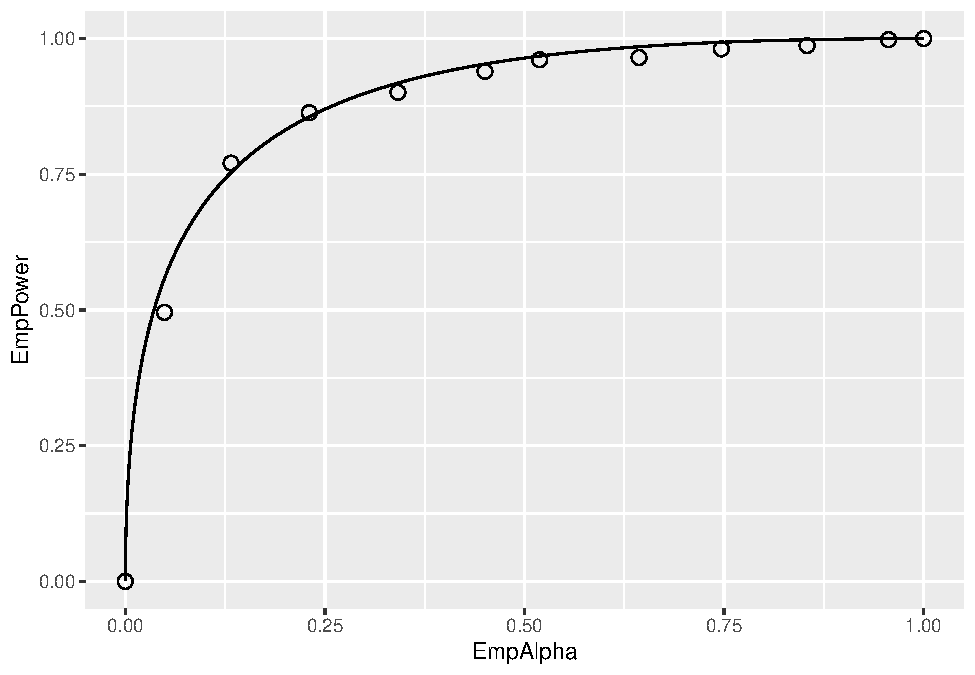
\includegraphics{08-hypothesis-testing_files/figure-latex/unnamed-chunk-7-1.pdf}

Relevant line numbers are shown above as comments. Line 6 creates two variables, \texttt{muNH} = 1.5 (the binormal model separation parameter under the NH) and \texttt{muAH} = 2.1 (the separation parameter under the AH). Under either hypotheses, the same diseased case standard deviation \texttt{sigma} = 1.3 and 50 non-diseased and 52 diseased cases are assumed. As before, lines 8 -- 14 use the ``brute force'' technique to determine population AUC and standard deviation of AUC under the NH condition. Line 16 defines the number of trials \texttt{T} = 2000. Line 17 creates a vector \texttt{mu} containing the NH and AH values defined at line 6. Line 18 creates \texttt{alphaArr}, a sequence of 10 equally spaced values in the range 0.05 to 0.95, which represent 10 values for \(\alpha\). Line 19 creates two arrays of length 10 each, named \texttt{EmpAlpha} and \texttt{EmpPower}, to hold the values of the observed Type-I error rate, i.e., empirical \(\alpha\), and the empirical power, respectively. The program will run \texttt{T} = 2000 NH and \texttt{T} = 2000 AH trials using as \(\alpha\) each successive value in \texttt{alphaArr} and save the observed Type-I error rates and observed powers to the arrays \texttt{EmpAlpha} and \texttt{EmpPower}, respectively.

Line 20 begins a for-loop in \texttt{a}, an index into \texttt{alphaArr.} Line 21 selects the appropriate value for \texttt{alpha} (0.05 on the first pass, 0.15 on the next pass, etc.). Line 22 initializes \texttt{reject{[}2,2000{]}} with zeroes, to hold the result of each trial; the first index corresponds to hypothesis \texttt{h} and the second to trial \texttt{t}. Line 23 begins a for-loop in \texttt{h}, with \texttt{h} = 1 corresponding to the NH and \texttt{h} = 2 to the AH. Line 24 begins a for-loop in \texttt{t}, the trial index. The code within this block is similar to previous examples. It simulates ratings, computes AUC, calculates the p-value, and saves a rejection of the NH as a one at the appropriate array location \texttt{reject{[}h,t{]}}. Lines 32 -- 33 calculate the empirical \(\alpha\) and empirical power for each value of \(\alpha\) in \texttt{alphaArr}. After padding the ends with zero and ones (the trivial points), the remaining lines plot the ``ROC within an ROC''.

Each of the circles in the figure corresponds to a specific value of \(\alpha\). For example the lowest non-trivial corresponds to \(\alpha\) = 0.05, for which the empirical \(\alpha\) is 0.049 and the corresponding empirical Power is 0.4955. True \(\alpha\) increases as the operating point moves up the plot, with empirical \(\alpha\) and empirical power increasing correspondingly. The \(\text{AUC}\) under this curve is determined by the effect size, defined as the difference between the AH and NH values of the separation parameter. If the effect size is zero, then the circles will scatter around the chance diagonal; the scatter will be consistent with the 2000 trials used to generate each coordinate of a point. As the effect size increases, the plot approaches the perfect ``ROC'', i.e., approaching the top-left corner. One could use AUC under this ``ROC'' as a measure of the incremental performance, the advantage being that it would be totally independent of \(\alpha\), but this would not be practical as it requires replication of the study under NH and AH conditions about 2000 times each and the entire process has to be repeated for several values of \(\alpha\). The purpose of this demonstration was to illustrate the concept behind Metz's profound remark.

It is time to move on to factors affecting statistical power in a single study.

\hypertarget{factors-affecting-statistical-power}{%
\subsection{Factors affecting statistical power}\label{factors-affecting-statistical-power}}

\begin{itemize}
\tightlist
\item
  Effect size: effect size is defined as the difference in \(\text{AUC}_{pop}\) values between the alternative hypothesis condition and the null hypothesis condition. Recall that \(\text{AUC}_{pop}\) is defined as the true or population value of the empirical ROC-AUC for the relevant hypothesis. One can use the ``cheat method'' to estimate it under the alternative hypothesis. The formalism is easier if one assumes it is equal to the asymptotic binormal model predicted value. The binormal model yields an estimate of the parameters, which only approach the population values in the asymptotic limit of a large number of cases. In the following, it is assumed that the parameters on the right hand side are the population values)
  It follows that effect size (ES) is given by (all quantities on the right hand side of Eqn. (8.13) are population values):
\end{itemize}

\begin{equation*} 
\text{AUC} = \Phi\left ( \frac{ \mu }{\sqrt{ 1 + \sigma^2}} \right )
\end{equation*}

It follows that effect size (ES) is given by (all quantities on the right hand side of above equation are population values):

\begin{equation*} 
ES = \Phi\left ( \frac{\mu_{AH}}{\sqrt{1+\sigma^2}} \right ) - \Phi\left ( \frac{\mu_{NH}}{\sqrt{1+\sigma^2}} \right )
\end{equation*}

\begin{Shaded}
\begin{Highlighting}[]
\NormalTok{EffectSize \textless{}{-}}\StringTok{ }\ControlFlowTok{function}\NormalTok{ (muNH, sigmaNH, muAH, sigmaAH)}
\NormalTok{\{}
\NormalTok{  ES \textless{}{-}}\StringTok{ }\KeywordTok{pnorm}\NormalTok{(muAH}\OperatorTok{/}\KeywordTok{sqrt}\NormalTok{(}\DecValTok{1}\OperatorTok{+}\NormalTok{sigmaAH}\OperatorTok{\^{}}\DecValTok{2}\NormalTok{)) }\OperatorTok{{-}}\StringTok{ }\KeywordTok{pnorm}\NormalTok{(muNH}\OperatorTok{/}\KeywordTok{sqrt}\NormalTok{(}\DecValTok{1}\OperatorTok{+}\NormalTok{sigmaNH}\OperatorTok{\^{}}\DecValTok{2}\NormalTok{))}
  \KeywordTok{return}\NormalTok{ (ES)}
\NormalTok{\}}

\NormalTok{seed \textless{}{-}}\StringTok{ }\DecValTok{1}\NormalTok{;}\KeywordTok{set.seed}\NormalTok{(seed)}
\NormalTok{muAH \textless{}{-}}\StringTok{ }\FloatTok{2.1} \CommentTok{\# NH value, defined previously, was mu = 1.5}

\NormalTok{T \textless{}{-}}\StringTok{ }\DecValTok{2000}
\NormalTok{alpha \textless{}{-}}\StringTok{ }\FloatTok{0.05} \CommentTok{\# size of test}
\NormalTok{reject =}\StringTok{ }\KeywordTok{array}\NormalTok{(}\DecValTok{0}\NormalTok{, }\DataTypeTok{dim =}\NormalTok{ T)}
\ControlFlowTok{for}\NormalTok{ (t }\ControlFlowTok{in} \DecValTok{1}\OperatorTok{:}\KeywordTok{length}\NormalTok{(reject)) \{  }
\NormalTok{  zk1 \textless{}{-}}\StringTok{ }\KeywordTok{rnorm}\NormalTok{(K1);zk2 \textless{}{-}}\StringTok{ }\KeywordTok{rnorm}\NormalTok{(K2, }\DataTypeTok{mean =}\NormalTok{ muAH, }\DataTypeTok{sd =}\NormalTok{ sigma)  }
\NormalTok{  AUC \textless{}{-}}\StringTok{ }\KeywordTok{Wilcoxon}\NormalTok{(zk1, zk2)  }
\NormalTok{  obsvdZ \textless{}{-}}\StringTok{ }\NormalTok{(AUC }\OperatorTok{{-}}\StringTok{ }\NormalTok{meanAUC)}\OperatorTok{/}\NormalTok{sigmaAUC}
\NormalTok{  p \textless{}{-}}\StringTok{ }\DecValTok{2}\OperatorTok{*}\KeywordTok{pnorm}\NormalTok{(}\OperatorTok{{-}}\KeywordTok{abs}\NormalTok{(obsvdZ)) }\CommentTok{\# p value for individual t}
  \ControlFlowTok{if}\NormalTok{ (p }\OperatorTok{\textless{}}\StringTok{ }\NormalTok{alpha) reject[t] =}\StringTok{ }\DecValTok{1} 
\NormalTok{\}}

\NormalTok{ObsvdTypeIErrRate \textless{}{-}}\StringTok{ }\KeywordTok{sum}\NormalTok{(reject)}\OperatorTok{/}\KeywordTok{length}\NormalTok{(reject)}
\NormalTok{CI \textless{}{-}}\StringTok{ }\KeywordTok{c}\NormalTok{(}\DecValTok{0}\NormalTok{,}\DecValTok{0}\NormalTok{);width \textless{}{-}}\StringTok{ }\OperatorTok{{-}}\KeywordTok{qnorm}\NormalTok{(alpha}\OperatorTok{/}\DecValTok{2}\NormalTok{)}
\NormalTok{CI[}\DecValTok{1}\NormalTok{] \textless{}{-}}\StringTok{ }\NormalTok{ObsvdTypeIErrRate }\OperatorTok{{-}}\StringTok{ }
\StringTok{  }\NormalTok{width}\OperatorTok{*}\KeywordTok{sqrt}\NormalTok{(ObsvdTypeIErrRate}\OperatorTok{*}\NormalTok{(}\DecValTok{1}\OperatorTok{{-}}\NormalTok{ObsvdTypeIErrRate)}\OperatorTok{/}\NormalTok{T)}
\NormalTok{CI[}\DecValTok{2}\NormalTok{] \textless{}{-}}\StringTok{ }\NormalTok{ObsvdTypeIErrRate }\OperatorTok{+}\StringTok{ }
\StringTok{  }\NormalTok{width}\OperatorTok{*}\KeywordTok{sqrt}\NormalTok{(ObsvdTypeIErrRate}\OperatorTok{*}\NormalTok{(}\DecValTok{1}\OperatorTok{{-}}\NormalTok{ObsvdTypeIErrRate)}\OperatorTok{/}\NormalTok{T)}
\KeywordTok{cat}\NormalTok{(}\StringTok{"obsvdPower = "}\NormalTok{, ObsvdTypeIErrRate, }\StringTok{"}\CharTok{\textbackslash{}n}\StringTok{"}\NormalTok{)}
\CommentTok{\#\textgreater{} obsvdPower =  0.489}
\KeywordTok{cat}\NormalTok{(}\StringTok{"95\% confidence interval = "}\NormalTok{, CI, }\StringTok{"}\CharTok{\textbackslash{}n}\StringTok{"}\NormalTok{)}
\CommentTok{\#\textgreater{} 95\% confidence interval =  0.4670922 0.5109078}
\KeywordTok{cat}\NormalTok{(}\StringTok{"Effect Size = "}\NormalTok{, }\KeywordTok{EffectSize}\NormalTok{(mu, sigma, muAH, sigma), }\StringTok{"}\CharTok{\textbackslash{}n}\StringTok{"}\NormalTok{)}
\CommentTok{\#\textgreater{} Effect Size =  0.08000617 0}
\end{Highlighting}
\end{Shaded}

The ES for the code above is 0.08 (in AUC units). It should be obvious that if effect size is zero, then power equals \(\alpha\). This is because then there is no distinction between the null and alternative hypotheses conditions. Conversely, as effect size increases, statistical power increases, the limiting value being unity, when every trial results in rejection of the null hypothesis. The reader should experiment with different values of \texttt{muAH} to be convinced of the truth of these statements.

\begin{itemize}
\tightlist
\item
  Sample size: increase the number of cases by a factor of two, and run the above code chunk.
\end{itemize}

\begin{verbatim}
#> pop NH mean AUC =  0.8594882 , pop NH sigma AUC =  0.02568252
#> num. non-diseased images =  100 num. diseased images =  104
#> obsvdPower =  0.313
#> 95% confidence interval =  0.2926772 0.3333228
#> Effect Size =  0.08000617 0
\end{verbatim}

So doubling the numbers of cases (both non-diseased and diseased) results in statistical power increasing from 0.509 to 0.844. Increasing the numbers of cases decreases \(\sigma_{\text{AUC}}\), the standard deviation of the empirical AUC. The new value of \(\sigma_{\text{AUC}}\) is 0.02947, which should be compared to the value 0.04177 for K1 = 50, K2 = 52. Recall that \(\sigma_{\text{AUC}}\) enters the denominator of the Z-statistic, so decreasing it will increase the probability of rejecting the null hypothesis.

\begin{itemize}
\tightlist
\item
  Alpha: Statistical power depends on \(alpha\). The results below are for two runs of the code, the first with the original value \(\alpha\) = 0.05, the second with \(\alpha\) = 0.01:
\end{itemize}

\begin{verbatim}
#> alpha =  0.05 obsvdPower =  0.1545 
#> alpha =  0.01 obsvdPower =  0.0265
\end{verbatim}

Decreasing \(\alpha\) results in decreased statistical power.

\hypertarget{HypothesisTestingComments}{%
\section{Comments}\label{HypothesisTestingComments}}

The Wilcoxon statistic was used to estimate the area under the ROC curve. One could have used the binormal model, introduced in Chapter 06, to obtain maximum likelihood estimates of the area under the binormal model fitted ROC curve. The reasons for choosing the simpler empirical area are as follows. (1) With continuous ratings and 102 operating points, the area under the empirical ROC curve is expected to be a close approximation to the fitted area. (2) With maximum likelihood estimation, the code would be more complex -- in addition to the fitting routine one would require a binning routine and that would introduce yet another variable in the analysis, namely the number of bins and how the bin boundaries were chosen. (3) The maximum likelihood fitting code can sometimes fail to converge, while the Wilcoxon method is always guaranteed to yield a result. The non-convergence issue is overcome by modern methods of curve fitting described in later chapters. (4) The aim was to provide an understanding of null hypothesis testing and statistical power without being bogged down in the details of curve fitting.

\hypertarget{why-alpha-is-chosen-as-5}\label{why-alpha-is-chosen-as-5}}

One might ask why \(\alpha\) is traditionally chosen to be 5\%. It is not a magical number, rather the result of a cost benefit tradeoff. Choosing too small a value of \(\alpha\) would result in greater probability \((1-\alpha)\) of the NH not being rejected, even when it is false. Sometimes it is important to detect a true difference between the measured AUC and the postulated value. For example, a new eye-laser surgery procedure is invented and the number of patients is necessarily small as one does not wish to subject a large number of patients to an untried procedure. One seeks some leeway on the Type-I error probability, possibly increasing it to \(\alpha\) = 0.1, in order to have a reasonable chance of success in detecting an improvement in performance due to better eyesight after the surgery. If the NH is rejected and the change is in the right direction, then that is good news for the researcher. One might then consider a larger clinical trial and set \(\alpha\) at the traditional 0.05, making up the lost statistical power by increasing the number of patients on which the surgery is tried.

If a whole branch of science hinges on the results of a study, such as discovering the Higg's Boson in particle physics, statistical significance is often expressed in multiples of the standard deviation (\(\sigma\)) of the normal distribution, with the significance threshold set at a much stricter level (e.g.~\(5\sigma\)). This corresponds to \(\alpha\) \textasciitilde{} 1 in 3.5 million (\texttt{1/pnorm(-5)} = 3.5 x 10\^{}6, a one-sided test of significance). There is an article in Scientific American (\url{https://blogs.scientificamerican.com/observations/five-sigmawhats-that/}) on the use of \(n\sigma\), where \texttt{n} is an integer, e.g.~5, to denote the significance level of a study, and some interesting anecdotes on why such high significance levels (ie., small \(\alpha\)) are used in some fields of research.

Similar concerns apply to manufacturing where the cost of a mistake could be the very expensive recall of an entire product line. For background on Six Sigma Performance, see \url{http://www.six-sigma-material.com/Six-Sigma.html}. An article downloaded 3/30/17 from \url{https://en.wikipedia.org/wiki/Six_Sigma} is included as supplemental material to this chapter (Six Sigma.pdf). It has an explanation of why \(6\sigma\) translates to one defect per 3.4 million opportunities (it has to do with short-term and long-term drifts in a process). In the author's opinion, looking at other fields offers a deeper understanding of this material than simply stating that by tradition one adopts alpha = 5\%.

Most observer performance studies, while important in the search for better imaging methods, are not of such ``earth-shattering'' importance, and it is somewhat important to detect true differences at a reasonable alpha, so alpha = 5\% and beta = 20\% represent a good compromise. If one adopted a \(5\sigma\) criterion, the NH would never be rejected, and progress in image quality optimization would come to a grinding halt. That is not to say that a \(5\sigma\) criterion cannot be used; rather if used, the number of patients needed to detect a reasonable difference (effect size) with 80\% probability would be astronomically large. Truth-proven cases are a precious commodity in observer performance studies. Particle physicists working on discovering the Higg's Boson can get away with \(5\sigma\) criterion because the number of independent observations and/or effect size is much larger than corresponding numbers in observer performance research.

\hypertarget{HypothesisTestingDiscussion}{%
\section{Discussion}\label{HypothesisTestingDiscussion}}

In most statistics books, the subject of hypothesis testing is demonstrated in different (i.e., non-ROC) contexts. That is to be expected since the ROC-analysis field is a small sub-specialty of statistics (Prof.~Howard E. Rockette, private communication, ca. 2002). Since this book is about ROC analysis, the author decided to use a demonstration using ROC analysis. Using a data simulator, one can ``cheat'' by conducting a very large number of simulations to estimate the population \(\text{AUC}\) under the null hypothesis. This permitted us to explore the related concepts of Type-I and Type-II errors within the context of ROC analysis. Ideally, both errors should be zero, but the nature of statistics leads one to two compromises. Usually one accepts a Type-I error capped at 5\% and a Type-II error capped at 20\%. These translate to \(\alpha\) = 0.05 and desired statistical power = 80\%. The dependence of statistical power on \(\alpha\), the numbers of cases and the effect size was explored.

In TBA Chapter 11 sample-size calculations are described that allow one to estimate the numbers of readers and cases needed to detect a specified difference in inter-modality AUCs with expected statistical power = \(1-\beta\). The word ``detect'' in the preceding sentence is shorthand for ``reject the NH with incorrect rejection probability capped at \(\alpha\)''.

This chapter also gives the first example of validation of a hypothesis testing method. Statisticians sometimes refer to this as showing a proposed test is a ``5\% test''. What is meant is that one needs to be assured that when the NH is true the probability of NH rejection is consistent with the expected value. Since the observed NH rejection rate over 2000 simulations is a random variable, one does not expect the NH rejection rate to exactly equal 5\%, rather the constructed 95\% confidence interval (also a random interval variable) should include the NH value with probability 1 - \(\alpha\).

Comparing a single reader's performance to a specified value is not a clinically interesting problem. The next few chapters describe methods for significance testing of multiple-reader multiple-case (MRMC) ROC datasets, consisting of interpretations by a group of readers of a common set of cases in typically two modalities. It turns out that the analyses yield variability estimates that permit sample size calculation. After all, sample size calculation is all about estimation of variability, the denominator of the z-statistic. The formulae will look more complex, as interest is not in determining the standard deviation of AUC, but in the standard deviation of the inter-modality reader-averaged AUC difference. However, the basic concepts remain the same.

\hypertarget{HypothesisTesting-references}{%
\section{References}\label{HypothesisTesting-references}}

\hypertarget{DBMAnalysisBkgrnd}{%
\chapter{DBM method background}\label{DBMAnalysisBkgrnd}}

\hypertarget{DBMAnalysisBkgrnd-introduction}{%
\section{Introduction}\label{DBMAnalysisBkgrnd-introduction}}

The term \emph{treatment} is generic for \emph{imaging system}, \emph{modality} or \emph{image processing}; \emph{reader} is generic for \emph{radiologist} or \emph{algorithmic observer}, e.g., a computer aided detection (CAD) or artificial intelligence (AI) algorithm. The previous chapter described analysis of a single ROC dataset and comparing the observed area \(AUC\) under the ROC plot to a specified value. Clinically this is not an interesting problem; rather, interest is usually in comparing performance of a group of readers interpreting a common set of cases in two or more treatments. Such data is termed multiple reader multiple case (MRMC). {[}An argument could be made in favor of the term ``multiple-treatment multiple-reader'', since ``multiple-case'' is implicit in any ROC analysis that takes into account correct and incorrect decisions on cases. However, the author will stick with existing terminology.{]} The basic idea is that by sampling a sufficiently large number of readers and cases one can draw conclusions that apply broadly to other readers of similar skill levels interpreting other similar case sets in the selected treatments. How one accomplishes this, termed MRMC analysis, is the subject of this chapter.

This chapter describes the first truly successful method of analyzing MRMC ROC data, namely the Dorfman-Berbaum-Metz (DBM) method \citep{RN204}. The other method, due to Obuchowski and Rockette \citep{RN1450}, is the subject of Chapter 10 (TBA). Both methods have been substantially improved by Hillis \citep{RN1866, RN1865, RN2508}. It is not an overstatement that ROC analysis came of age with the methods described in this chapter. Prior to the techniques described here, one knew of the existence of sources of variability affecting a measured \(AUC\) value, as discussed in (book) Chapter 07, but then-known techniques \citep{RN412} for estimating the corresponding variances and correlations were impractical.

\hypertarget{historical-background}{%
\subsection{Historical background}\label{historical-background}}

The author was thrown (unprepared) into the methodology field ca. 1985 when, as a junior faculty member, he undertook comparing a prototype digital chest-imaging device (Picker International, ca. 1983) vs.~an optimized analog chest-imaging device at the University of Alabama at Birmingham. At the outset a decision was made to use free-response ROC methodology instead of ROC, as the former accounted for lesion localization, and the author and his mentor, Prof.~Gary T. Barnes, were influenced in that decision by a publication \citep{RN2453} to be described in (book) Chapter 12. Therefore, instead of ROC-AUC one had lesion-level sensitivity at a fixed number of location level false positives per case as the figure-of-merit (FOM). Details of the FOM are not relevant at this time. Suffice to state that methods described in this chapter, which had not been developed in 1983, while developed for analyzing reader-averaged inter-treatment ROC-AUC differences, \emph{apply to any scalar FOM}. While the author was successful at calculating confidence intervals (this is the heart of what is loosely termed \emph{statistical analysis}) and publishing the work \citep{RN621} using techniques described in a book \citep{RN412} titled ``Evaluation of Diagnostic Systems: Methods from Signal Detection Theory'', subsequent attempts at applying these methods in a follow-up paper \citep{RN620} led to negative variance estimates (private communication, Dr.~Loren Niklason, ca. 1985). With the benefit of hindsight, negative variance estimates are not that uncommon and the method to be described in this chapter has to deal with that possibility.

The methods \citep{RN412} described in the cited book involved estimating the different variability components -- case sampling, between-reader and within-reader variability. Between-reader and within-reader variability (the two cannot be separated as discussed in (book) Chapter 07) could be estimated from the variance of the \(AUC\) values corresponding to the readers interpreting the cases within a treatment and then averaging the variances over all treatments. Estimating case-sampling and within-reader variability required splitting the dataset into a few smaller subsets (e.g., a case set with 60 cases might be split into 3 sub-sets of 20 cases each), analyzing each subset to get an \(AUC\) estimate, calculating the variance of the resulting \(AUC\) values \citep{RN412} and scaling the result to the original case size. Because it was based on few values, the estimate was inaccurate, and the already case-starved original dataset made it difficult to estimate AUCs for the subsets; moreover, the division into subsets was at the discretion of the researcher, and therefore unlikely to be reproduced by others. Estimating within-reader variability required re-reading the entire case set, or at least a part of it. ROC studies have earned a deserved reputation for taking much time to complete, and having to re-read a case set was not a viable option. {[}Historical note: the author recalls a barroom conversation with Dr.~Thomas Mertelmeir after the conclusion of an SPIE meeting ca. 2004, where Dr.~Mertelmeir commiserated mightily, over several beers, about the impracticality of some of the ROC studies required of imaging device manufacturers by the FDA.{]}

\hypertarget{the-wagner-analogy}{%
\subsection{The Wagner analogy}\label{the-wagner-analogy}}

An important objective of modality comparison studies is to estimate the variance of the difference in reader-averaged AUCs between the treatments. For two treatments one sums the reader-averaged variance in each treatment and subtracts twice the covariance (a scaled version of the correlation). Therefore, in addition to estimating variances, one needs to estimate correlations. Correlations are present due to the common case set interpreted by the readers in the different treatments. If the correlation is large, i.e., close to unity, then the individual treatment variances tend to cancel, making the constant treatment-induced difference easier to detect. The author recalls a vivid analogy used by the late Dr.~Robert F. Wagner to illustrate this point at an SPIE meeting ca. 2008. To paraphrase him, \emph{consider measuring from shore the heights of the masts on two adjacent boats in a turbulent ocean. Because of the waves, the heights, as measured from shore, are fluctuating wildly, so the variance of the individual height measurements is large. However, the difference between the two heights is likely to be relatively constant, i.e., have small variance. This is because the wave that causes one mast's height to increase also increases the height of the other mast.}

\hypertarget{the-shortage-of-numbers-to-analyze-and-a-pivotal-breakthrough}{%
\subsection{The shortage of numbers to analyze and a pivotal breakthrough}\label{the-shortage-of-numbers-to-analyze-and-a-pivotal-breakthrough}}

\emph{The basic issue was that the calculation of \(AUC\) reduces the relatively large number of ratings of a set of non-diseased and diseased cases to a single number.} For example, after completion of an ROC study with 5 readers and 100 non-diseased and 100 diseased cases interpreted in two treatments, the data is reduced to just 10 numbers, i.e., five readers times two treatments. It is difficult to perform statistics with so few numbers. The author recalls a conversation with Prof.~Kevin Berbaum at a Medical Image Perception Society meeting in Tucson, Arizona, ca. 1997, in which he described the basic idea that forms the subject of this chapter. Namely, using jackknife pseudovalues (to be defined below) as individual case-level figures of merit. This, of course, greatly increases the amount of data that one can work with; instead of just 10 numbers one now has 2,000 pseudovalues (2 x 5 x 200). If one assumes the pseudovalues behave essentially as case-level data, then by assumption they are independent and identically distributed, and therefore satisfy the conditions for application of standard analysis of variance (ANOVA) techniques. {[}This assumption has been much criticized and is the basis for some preferring alternate approaches - but, as Hillis has stated, and I paraphrase, the pseudovalue based method ``works'', but lacks sufficient rigor.{]} The relevant paper had already been published in 1992 but other projects and lack of formal statistical training kept the author from fully appreciating this work until later.

For the moment I restrict to fully paired data (i.e., each case is interpreted by all readers in all treatments). There is a long history of how this field has evolved and the author cannot do justice to all methods that are currently available. Some of the methods \citep{RN1441, RN2013, RN1451} have the advantage that they can handle explanatory variables (termed covariates) that could influence performance, e.g., years of experience, types of cases, etc. Other methods are restricted to specific choices of FOM. Specifically, the probabilistic approach \citep{RN2253, RN2254, RN2351, RN2080} is restricted to the empirical \(AUC\) under the ROC curve, and is not applicable to other FOMs, e.g., parametrically fitted ROC AUCs or, more importantly, to location specific paradigm FOMs. Instead, the author will focus on methods for which software is readily available (i.e., freely on websites), which have been widely used (the method that the author is about to describe has been used in several hundred publications) and validated via simulations, and which apply to any scalar figure of merit, and therefore widely applicable, for example, to location specific paradigms.

\hypertarget{organization-of-chapter}{%
\subsection{Organization of chapter}\label{organization-of-chapter}}

The concepts of reader and case populations, introduced in (book) Chapter 07, are recapitulated. A distinction is made between \emph{fixed} and \emph{random} factors -- statistical terms with which one must become familiar. Described next are three types of analysis that are possible with MRMC data, depending on which factors are regarded as random and which as fixed. The general approach to the analysis is described. Two methods of analysis are possible: the jackknife pseudovalue-based approach detailed in this chapter and an alternative approach is detailed in Chapter 10. The Dorfman-Berbaum-Metz (DBM) model for the jackknife pseudovalues is described that incorporates different sources of variability and correlations possible with MRMC data. Calculation of ANOVA-related quantities, termed mean squares, from the pseudovalues, are described followed by the significance testing procedure for testing the null hypothesis of no treatment effect. A relevant distribution used in the analysis, namely the F-distribution, is illustrated with R examples. The decision rule, i.e., whether to reject the NH, calculation of the ubiquitous p-value, confidence intervals and how to handle multiple treatments is illustrated with two datasets, one an older ROC dataset that has been widely used to demonstrate advances in ROC analysis, and the other a recent dataset involving evaluation of digital chest tomosynthesis vs.~conventional chest imaging. The approach to validation of DBM analysis is illustrated with an R example. The chapter concludes with a section on the meaning of the pseudovalues. The intent is to explain, at an intuitive level, why the DBM method ``works'', even though use of pseudovalues has been questioned at the conceptual level. For organizational reasons and space limitations, details of the software are relegated to Online Appendices, but they are essential reading, preferably in front of a computer running the online software that is part of this book. The author has included material here that may be obvious to statisticians, e.g., an explanation of the Satterthwaite approximation, but are expected to be helpful to others from non-statistical backgrounds.

\hypertarget{DBMAnalysisBkgrnd-random-fixed-factors}{%
\section{Random and fixed factors}\label{DBMAnalysisBkgrnd-random-fixed-factors}}

\emph{This paragraph introduces some analysis of variance (ANOVA) terminology. Treatment, reader and case are factors with different numbers of levels corresponding to each factor. For an ROC study with two treatments, five readers and 200 cases, there are two levels of the treatment factor, five levels of the reader factor and 200 levels of the case factor. If a factor is regarded as fixed, then the conclusions of the analysis apply only to the specific levels of the factor used in the study. If a factor is regarded as random, the levels of the factor are regarded as random samples from a parent population of the corresponding factor, and conclusions regarding specific levels are not allowed; rather, conclusions apply to the distribution from which the levels were sampled.}

ROC MRMC studies require a sample of cases and interpretations by one or more readers in one or more treatments (in this book the term \emph{multiple} includes as a special case \emph{one}). A study is never conducted on a sample of treatments. It would be nonsensical to image patients using a ``sample'' of all possible treatments. Every variation of an imaging technique (e.g., different kilovoltage or kVp) or display method (e.g., window-level setting) or image processing techniques qualifies as a distinct treatment. The number of possible treatments is very large, and, from a practical point of view, most of them are uninteresting. Rather, interest is in comparing two or more (a few at most) treatments that, based on preliminary studies, are clinically interesting. One treatment may be computed tomography, the other magnetic resonance imaging, or one may be interested in comparing a standard image processing method to a newly proposed one, or one may be interested in comparing CAD to a group of readers.

This brings out an essential difference between how cases, readers and treatments have to be regarded in the variability estimation procedure. Cases and readers are usually regarded as random factors (there has to be at least one random factor -- if not, there are no sources of variability and nothing to apply statistics to!), while treatments are regarded as fixed factors. The random factors contribute variability, but the fixed factors do not, rather they contribute constant shifts in performance. The terms \emph{fixed} and \emph{random} factors are used in this specific sense, and are derived, in turn, from ANOVA methods in statistics. With two or more treatments, there are shifts in performance of treatments relative to each other, that one seeks to assess the significance of, against a background of noise contributed by the random factors. If the shifts are sufficiently large compared to the noise, then one can state, with some certainty, that they are real. Quantifying the last statement uses the methods of hypothesis testing introduced in Chapter \ref{HypothesisTesting}.

\hypertarget{DBMAnalysisBkgrnd-reader-case-populations}{%
\section{Reader and case populations}\label{DBMAnalysisBkgrnd-reader-case-populations}}

Consider a sample of \(J\) readers. Conceptually there is a reader-population, modeled as a normal distribution \(\theta_j \sim N\left ( \theta_{\bullet\{1\}}, \sigma_{br+wr}^{2} \right )\), describing the variation of skill-level of readers. Here \(\theta\) is a generic FOM. Each reader \(j\) is characterized by a different value of \(\theta_j\), \(j=1,2,...J\) and one can conceptually think of a bell-shaped curve with variance \(\sigma_{br+wr}^{2}\) describing between-reader variability of the readers. A large variance implies large spread in reader skill levels.

Likewise, there is a case-population, also modeled as a normal distribution, describing the variations in difficulty levels of the patients. One actually has two unit-variance distributions, one for non-diseased and one for diseased cases, characterized by a separation parameter. The separation parameter is scaled (i.e., normalized) by the standard deviation of each distribution (assumed equal). Each distribution has unit variance. Conceptually an easy case set has a larger than usual scaled separation parameter while a difficult case set has a smaller than usual scaled separation parameter. The distribution of the scaled separation parameter can be modeled as a bell-shaped curve \(\theta_{\{c\}} \sim N\left ( \theta_{\{\bullet\}}, \sigma_{cs+wr}^{2} \right )\) with variance \(\sigma_{cs+wr}^{2}\) describing the variations in difficulty levels of different case samples. Note the need for the case-set index, introduced in (book) Chapter 07, to specify the separation parameter for a specific case-set (in principle a \(j\)-index is also needed as one cannot have an interpretation without a reader; for now it is suppressed. A small variance \(\sigma_{cs}^{2}\) implies the different case sets have similar difficulty levels while a larger variance would imply a larger spread in difficulty levels. Just as the previous paragraph described reader-varibility, this paragraph has described case-variability.

\emph{Anytime one has a common random component to two measurements, the measurements are correlated.} In the Wagner analogy, the common component is the random height, as a function of time, of a wave, which contributes the same amount to both height measurements (since the boats are adjacent). Since the readers interpret a common case set in all treatments one needs to account for various types of correlations that are potentially present. These occur due to the various types of pairings that can occur with MRMC data, where each pairing implies the presence of a common component to the measurements: (a) the same reader interpreting the \emph{same cases} in different treatments, (b) different readers interpreting the \emph{same cases} in the same treatment and (c) different readers interpreting the \emph{same cases} in different treatments. These pairings are more clearly elucidated in (book) Chapter 10. The current chapter uses jackknife pseudovalue based analysis to model the variances and the correlations. Hillis has shown that the two approaches are essentially equivalent \citep{RN1866}.

\hypertarget{DBMAnalysisBkgrnd-threeAnalyses}{%
\section{Three types of analyses}\label{DBMAnalysisBkgrnd-threeAnalyses}}

\emph{MRMC analysis aims to draw conclusions regarding the significances of inter-treatment shifts in performance. Ideally a conclusion (i.e., a difference is significant) should generalize to the respective populations from which the random samples were obtained. In other words, the idea is to generalize from the observed samples to the underlying populations. Three types of analyses are possible depending on which factor(s) one regards as random and which as fixed: random-reader random-case (RRRC), fixed-reader random-case (FRRC) and random-reader fixed-case (RRFC). If a factor is regarded as random, then the conclusion of the study applies to the population from which the levels of the factor were sampled. If a factor is regarded as fixed, then the conclusion applies only to the specific levels of the sampled factor. For example, if reader is regarded as a random factor, the conclusion generalizes to the reader population from which the readers used in the study were obtained. If reader is regarded as a fixed factor, then the conclusion applies to the specific readers that participated in the study. Regarding a factor as fixed effectively ``freezes out'' the sampling variability of the population and interest then centers only on the specific levels of the factor used in the study. Likewise, treating case as a fixed factor means the conclusion of the study is specific to the case-set used in the study.}

\hypertarget{DBMAnalysisBkgrnd-approach}{%
\section{General approach}\label{DBMAnalysisBkgrnd-approach}}

This section provides an overview of the steps involved in analysis of MRMC data. Two approaches are described in parallel: a figure of merit (FOM) derived jackknife pseudovalue based approach, detailed in this chapter and an FOM based approach, detailed in the next chapter. The analysis proceeds as follows:

\begin{enumerate}
\def\labelenumi{\arabic{enumi}.}
\tightlist
\item
  A FOM is selected: \emph{the selection of FOM is the single-most critical aspect of analyzing an observer performance study}. The selected FOM is denoted \(\theta\). The FOM has to be an objective scalar measure of performance with larger values characterizing better performance. {[}The qualifier ``larger'' is trivially satisfied; if the figure of merit has the opposite characteristic, a sign change is all that is needed to bring it back to compliance with this requirement.{]} Examples are empirical \(AUC\), the binormal model-based estimate \(A_z\) , other advance method based estimates of \(AUC\), sensitivity at a predefined value of specificity, etc. An example of a FOM requiring a sign-change is \(FPF\) at a specified \(TPF\), where smaller values signify better performance.
\item
  For each treatment \(i\) and reader \(j\) the figure of merit \(\theta_{ij}\) is estimated from the ratings data. Repeating this over all treatments and readers yields a matrix of observed values \(\theta_{ij}\). This is averaged over all readers in each treatment yielding \(\theta_{i\bullet}\). The observed effect-size \(ES_{obs}\) is defined as the difference between the reader-averaged FOMs in the two treatments, i.e., \(ES_{obs} = \theta_{2\bullet}-\theta_{1\bullet}\). While extensible to more than two treatments, the explanation is more transparent by restricting to two modalities.
\item
  If the magnitude of \(ES_{obs}\) is ``large'' one has reason to suspect that there might indeed be a significant difference in AUCs between the two treatments, where \emph{significant} is used in the sense of (book) Chapter 08. Quantification of this statement, specifically how large is ``large'', requires the conceptually more complex steps described next.

  \begin{itemize}
  \tightlist
  \item
    In the DBM approach, the subject of this chapter, jackknife pseudovalues are calculated as described in Chapter 08. A standard ANOVA model with uncorrelated errors is used to model the pseudovalues.
  \item
    In the OR approach, the subject of the next chapter, the FOM is modeled directly using a custom ANOVA model with correlated errors.
  \end{itemize}
\item
  Depending on the selected method of modeling the data (pseudovalue vs.~FOM) a statistical model is used which includes parameters modeling the true values in each treatment, and expected variations due to different variability components in the model, e.g., between-reader variability, case-sampling variability, interactions (e.g., allowing for the possibility that the random effect of a given reader could be treatment dependent) and the presence of correlations (between pseudovalues or FOMs) because of the pairings inherent in the interpretations.
\item
  In RRRC analysis one accounts for randomness in readers and cases. In FRRC analysis one regards reader as a fixed factor. In RRFC analysis one regards the case-sample (set of cases) as a fixed factor. The statistical model depends on the type of analysis.
\item
  The parameters of the statistical model are estimated from the observed data.
\item
  The estimates are used to infer the statistical distribution of the observed effect size, \(ES_{obs}\), regarded as a realization of a random variable, under the null hypothesis (NH) that the true effect size is zero.
\item
  Based on this statistical distribution, and assuming a two-sided test, the probability (this is the oft-quoted p-value) of obtaining an effect size at least as extreme as that actually observed, is calculated, as in (book) Chapter 08.
\item
  If the p-value is smaller than a preselected value, denoted \(\alpha\), one declares the treatments different at the \(\alpha\) - significance level. The quantity \(\alpha\) is the control (or ``cap'') on the probability of making a Type I error, defined as rejecting the NH when it is true. It is common to set \(\alpha\) = 0.05 but depending on the severity of the consequences of a Type I error, as discussed in (book) Chapter 08, one might consider choosing a different value. Notice that \(\alpha\) is a pre-selected number while the p-value is a realization (observation) of a random variable.
\item
  For a valid statistical analysis, the empirical probability \(\alpha_{emp}\) over many (typically 2000) independent NH datasets, that the p-value is smaller than \(\alpha\), should equal \(\alpha\) to within statistical uncertainty.
\end{enumerate}

\hypertarget{DBMAnalysisBkgrnd-summary}{%
\section{Summary TBA}\label{DBMAnalysisBkgrnd-summary}}

This chapter has detailed analysis of MRMC ROC data using the DBM method. A reason for the level of detail is that almost all of the material carries over to other data collection paradigms, and a thorough understanding of the relatively simple ROC paradigm data is helpful to understanding the more complex ones.

DBM has been used in several hundred ROC studies (Prof.~Kevin Berbaum, private communication ca. 2010). While the method allows generalization of a study finding, e.g., rejection of the NH, to the population of readers and cases, the author believes this is sometimes taken too literally. If a study is done at a single hospital, then the radiologists tend to be more homogenous as compared to sampling radiologists from different hospitals. This is because close interactions between radiologists at a hospital tend to homogenize reading styles and performance. A similar issue applies to patient characteristics, which are also expected to vary more between different geographical locations than within a given location served by the hospital. This means is that single hospital study based p-values may tend to be biased downwards, declaring differences that may not be replicable if a wider sampling ``net'' were used using the same sample size. The price paid for a wider sampling net is that one must use more readers and cases to achieve the same sensitivity to genuine treatment effects, i.e., statistical power (i.e., there is no ``free-lunch'').

A third MRMC ROC method, due to Clarkson, Kupinski and Barrett19,20, implemented in open-source JAVA software by Gallas and colleagues22,44 (\url{http://didsr.github.io/iMRMC/}) is available on the web. Clarkson et al19,20 provide a probabilistic rationale for the DBM model, provided the figure of merit is the empirical \(AUC\). The method is elegant but it is only applicable as long as one is using the empirical AUC as the figure of merit (FOM) for quantifying observer performance. In contrast the DBM approach outlined in this chapter, and the approach outlined in the following chapter, are applicable to any scalar FOM. Broader applicability ensures that significance-testing methods described in this, and the following chapter, apply to other ROC FOMs, such as binormal model or other fitted AUCs, and more importantly, to other observer performance paradigms, such as free-response ROC paradigm. An advantage of the Clarkson et al.~approach is that it predicts truth-state dependence of the variance components. One knows from modeling ROC data that diseased cases tend to have greater variance than non-diseased ones, and there is no reason to suspect that similar differences do not exist between the variance components.

Testing validity of an analysis method via simulation testing is only as good as the simulator used to generate the datasets, and this is where current research is at a bottleneck. The simulator plays a central role in ROC analysis. In the author's opinion this is not widely appreciated. In contrast, simulators are taken very seriously in other disciplines, such as cosmology, high-energy physics and weather forecasting. The simulator used to validate3 DBM is that proposed by Roe and Metz39 in 1997. This simulator has several shortcomings. (a) It assumes that the ratings are distributed like an equal-variance binormal model, which is not true for most clinical datasets (recall that the b-parameter of the binormal model is usually less than one). Work extending this simulator to unequal variance has been published3. (b) It does not take into account that some lesions are not visible, which is the basis of the contaminated binormal model (CBM). A CBM model based simulator would use equal variance distributions with the difference that the distribution for diseased cases would be a mixture distribution with two peaks. The radiological search model (RSM) of free-response data, Chapter 16 \&17 also implies a mixture distribution for diseased cases, and it goes farther, as it predicts some cases yield no z-samples, which means they will always be rated in the lowest bin no matter how low the reporting threshold. Both CBM and RSM account for truth dependence by accounting for the underlying perceptual process. (c) The Roe-Metz simulator is out dated; the parameter values are based on datasets then available (prior to 1997). Medical imaging technology has changed substantially in the intervening decades. (d) Finally, the methodology used to arrive at the proposed parameter values is not clearly described. Needed is a more realistic simulator, incorporating knowledge from alternative ROC models and paradigms that is calibrated, by a clearly defined method, to current datasets.

Since ROC studies in medical imaging have serious health-care related consequences, no method should be used unless it has been thoroughly validated. Much work still remains to be done in proper simulator design, on which validation is dependent.

\hypertarget{DBMAnalysisBkgrnd-references}{%
\section{References}\label{DBMAnalysisBkgrnd-references}}

\hypertarget{DBMAnalysisSigtesting}{%
\chapter{Significance Testing using the DBM Method}\label{DBMAnalysisSigtesting}}

DBM = Dorfman Berbaum Metz

\hypertarget{the-dbm-sampling-model}{%
\section{The DBM sampling model}\label{the-dbm-sampling-model}}

The figure-of-merit has three indices:

\begin{itemize}
\tightlist
\item
  A treatment index \(i\), where \(i\) runs from 1 to \(I\), where \(I\) is the total number of treatments.\\
\item
  A reader index \(j\), where \(j\) runs from 1 to \(J\), where \(J\) is the total number of readers.\\
\item
  The case-sample index \(\{c\}\), where \(\{1\}\) i.e., \(c\) = 1, denotes a set of cases, \(K_1\) non-diseased and \(K_2\) diseased, interpreted by all readers in all treatments, and other integer values of \(c\) correspond to other independent sets of cases that, although not in fact interpreted by the readers, could potentially be ``interpreted'' using resampling methods such as the bootstrap or the jackknife.
\end{itemize}

The approach \citep{RN204} taken by DBM was to use the jackknife resampling method to calculate FOM pseudovalues \({Y'}_{ijk}\) defined by (the reason for the prime will become clear shortly):

\begin{equation}
Y'_{ijk}=K\theta_{ij}-(K-1)\theta_{ij(k)}
\label{eq:pseudoValPrime}
\end{equation}

Here \(\theta_{ij}\) is the estimate of the figure-of-merit for reader \(j\) interpreting all cases in treatment \(i\) and \(\theta_{ij(k)}\) is the corresponding figure of merit with case \(k\) \emph{deleted} from the analysis. To keep the notation compact the case-sample index \(\{1\}\) on every figure of merit symbol is suppressed.

Recall from book Chapter 07 that the jackknife is a way of teasing out the case-dependence: the left hand side of Equation \eqref{eq:pseudoValPrime} has a case index \(k\), with \(k\) running from 1 to \(K\), where \(K\) is the total number of cases: \(K=K_1+K_2\).

Hillis et al \citep{RN1866} proposed a centering transformation on the pseudovalues (he terms it ``normalized'' pseudovalues, but to me ``centering'' is a more accurate and descriptive term - \emph{Normalize: (In mathematics) multiply (a series, function, or item of data) by a factor that makes the norm or some associated quantity such as an integral equal to a desired value (usually 1). New Oxford American Dictionary, 2016}):

\begin{equation}
Y_{ijk}=Y'_{ijk}+\left (\theta_{ij} - Y'_{ij\bullet}  \right )
\label{eq:pValCentered}
\end{equation}

\textbf{Note: the bullet symbol denotes an average over the corresponding index.}

The effect of this transformation is that the average of the centered pseudovalues over the case index is identical to the corresponding estimate of the figure of merit:

\begin{equation}
Y_{ij\bullet}=Y'_{ij\bullet}+\left (\theta_{ij} - Y'_{ij\bullet}  \right )=\theta_{ij}
\label{eq:EffectOfCentering}
\end{equation}

This has the advantage that all confidence intervals are properly centered. The transformation is unnecessary if one uses the Wilcoxon as the figure-of-merit, as the pseudovalues calculated using the Wilcoxon as the figure of merit are ``naturally'' centered, i.e.,

\(\theta_{ij} - Y'_{ij\bullet} = 0\)

\emph{It is understood that, unless explicitly stated otherwise, all calculations from now on will use centered pseudovalues.}

Consider \(N\) replications of a MRMC study, where a replication means repetition of the study with the same treatments, readers and case-set \(\{1\}\). For \(N\) replications per treatment-reader-case combination, the DBM model for the pseudovalues is (\(n\) is the replication index, usually \(n\) = 1, but kept here for now):

\begin{equation}
Y_{n(ijk)}  = \mu + \tau_i+ R_j + C_k + (\tau R)_{ij}+ (\tau C)_{ik}+ (R C)_{jk} + (\tau RC)_{ijk}+ \epsilon_{n(ijk)} 
\label{eq:DefDBMModel}
\end{equation}

The term \(\mu\) is a constant. By definition, the treatment effect \(\tau_i\) is subject to the constraint:

\begin{equation}
\sum_{i=1}^{I}\tau_i=0\Rightarrow \tau_\bullet=0
\label{eq:constraintTau}
\end{equation}

This constraint ensures that \(\mu\) has the interpretation of the average of the pseudovalues over treatments, readers and cases.

The (nesting) notation for the replication index, i.e., \(n(ijk)\), implies \(n\) observations for treatment-reader-case combination \(ijk\). With no replications (\(N\) = 1) it is convenient to omit the n-symbol.

The parameter \(\tau_i\) is estimated as follows:

\begin{equation}
Y_{ijk} \equiv Y_{1(ijk)}\\
\tau_i = Y_{i \bullet \bullet} -Y_{\bullet \bullet \bullet} 
\label{eq:estimatingTau}
\end{equation}

\emph{The basic assumption of the DBM model is that the pseudovalues can be regarded as independent and identically distributed observations. That being the case, the pseudovalues can be analyzed by standard ANOVA techniques.} Since pseduovalues are computed from a common dataset, this assumption is, non-intuitive. However, for the special case of Wilcoxon figure of merit, it is justified.

\hypertarget{explanation-of-terms-in-the-model}{%
\subsection{Explanation of terms in the model}\label{explanation-of-terms-in-the-model}}

The right hand side of Eqn. \eqref{eq:pseudoValPrime} consists of one fixed and 7 random effects. The current analysis assumes readers and cases as random factors (RRRC), so by definition \(R_j\) and \(C_k\) are random effects, and moreover, any term that includes a random factor is a random effect; for example, \((\tau R)_{ij}\) is a random effect because it includes the \(R\) factor. Here is a list of the random terms:

\begin{equation}
R_j, C_k, (\tau R)_{ij}, (\tau C)_{ik}, (RC)_{jk},  (\tau RC)_{ijk},  \epsilon_{ijk}
\label{eq:DBMRandomTerms}
\end{equation}

\textbf{Assumption:} Each of the random effects is modeled as a random sample from mutually independent zero-mean normal distributions with variances as specified below:

\begin{align}
\left.\begin{array}{rll}
{R_j}&\sim& N\left ( 0,\sigma_{R}^{2} \right ) \\[0.5em]
{C_k}&\sim& N\left ( 0,\sigma_{C}^{2} \right ) \\[0.5em]
{(\tau R)_{ij}}&\sim& N\left ( 0,\sigma_{\tau R}^{2} \right ) \\[0.5em]
{(\tau C)_{ik}}&\sim& N\left ( 0,\sigma_{\tau C}^{2} \right ) \\[0.5em]
{(RC)_{jk}}&\sim& N\left ( 0,\sigma_{RC}^{2} \right ) \\[0.5em]
{(\tau RC)_{ijk}}&\sim& N\left ( 0,\sigma_{\tau RC}^{2} \right ) \\[0.5em]
\epsilon_{ijk} &\sim& N\left ( 0,\sigma_{\epsilon}^{2} \right )
\end{array}\right\}
\label{eq:samplingOfDbmTerms}
\end{align}

Equation \eqref{eq:samplingOfDbmTerms} defines the meanings of the variance components appearing in Equation \eqref{eq:DBMRandomTerms}. One could have placed a \(Y\) subscript (or superscript) on each of the variances, as they describe fluctuations of the pseudovalues, not FOM values. However, this tends to clutter the notation. So here is the convention:

\textbf{Unless explicitly stated otherwise, all variance symbols in this chapter refer to pseudovalues. }
Another convention: \((\tau R)_{ij}\) is \emph{not} the product of the treatment and reader factors, rather it is a single factor, namely the treatment-reader factor with \(IJ\) levels, subscripted by the index \(ij\) and similarly for the other product-like terms in Equation \eqref{eq:samplingOfDbmTerms}.

\hypertarget{meanings-of-variance-components-in-the-dbm-model-tba-this-section-can-be-improved}{%
\subsection{\texorpdfstring{Meanings of variance components in the DBM model (\textbf{TBA this section can be improved})}{Meanings of variance components in the DBM model (TBA this section can be improved)}}\label{meanings-of-variance-components-in-the-dbm-model-tba-this-section-can-be-improved}}

The variances defined in \eqref{eq:samplingOfDbmTerms} are collectively termed \emph{variance components}. Specifically, they are jackknife pseudovalue variance components, to be distinguished from figure of merit (FOM) variance components to be introduced in TBA Chapter 10. They are in order: \(\sigma_{R}^{2} ,\sigma_{C}^{2} \sigma_{\tau R}^{2},\sigma_{\tau C}^{2},\sigma_{RC}^{2}, \sigma_{\tau RC}^{2},\sigma_{\epsilon}^{2}\). They have the following meanings.

\begin{itemize}
\tightlist
\item
  The term \(\sigma_{R}^{2}\) is the variance of readers that is independent of treatment or case, which are modeled separately. It is not to be confused with the terms \(\sigma_{br+wr}^{2}\) and \(\sigma_{cs+wr}^{2}\) used in §9.3, which describe the variability of \(\theta\) measured under specified conditions. {[}A jackknife pseudovalue is a weighted difference of FOM like quantities, TBA \eqref{eq:pseudoValPrime}. Its meaning will be explored later. For now, \emph{a pseudovalue variance is distinct from a FOM variance}.{]}
\item
  The term \(\sigma_{C}^{2}\) is the variance of cases that is independent of treatment or reader.
\item
  The term \(\sigma_{\tau R}^{2}\) is the treatment-dependent variance of readers that was excluded in the definition of \(\sigma_{R}^{2}\). If one were to sample readers and treatments for the same case-set, the net variance would be \(\sigma_{R}^{2}+\sigma_{\tau R}^{2}+\sigma_{\epsilon}^{2}\).
\item
  The term \(\sigma_{\tau C}^{2}\) is the treatment-dependent variance of cases that was excluded in the definition of \(\sigma_{C}^{2}\). So, if one were to sample cases and treatments for the same readers, the net variance would be \(\sigma_{C}^{2}+\sigma_{\tau C}^{2}+\sigma_{\epsilon}^{2}\).
\item
  The term \(\sigma_{RC}^{2}\) is the treatment-independent variance of readers and cases that were excluded in the definitions of \(\sigma_{R}^{2}\) and \(\sigma_{C}^{2}\). So, if one were to sample readers and cases for the same treatment, the net variance would be \(\sigma_{R}^{2}+\sigma_{C}^{2}+\sigma_{RC}^{2}+\sigma_{\epsilon}^{2}\).
\item
  The term \(\sigma_{\tau RC}^{2}\) is the variance of treatments, readers and cases that were excluded in the definitions of all the preceding terms in TBA \eqref{eq:pseudoValPrime}. So, if one were to sample treatments, readers and cases the net variance would be \(\sigma_{R}^{2}+\sigma_{C}^{2}+\sigma_{\tau C}^{2}+\sigma_{RC}^{2}+\sigma_{\tau RC}^{2}+\sigma_{\epsilon}^{2}\).
\item
  The last term, \(\sigma_{\epsilon}^{2}\) describes the variance arising from different replications of the study using the same treatments, readers and cases. Measuring this variance requires repeating the study several (\(N\)) times with the same treatments, readers and cases, and computing the variance of \(Y_{n(ijk)}\) , where the additional \(n\)-index refers to true replications, \(n\) = 1, 2, \ldots, \(N\).
\end{itemize}

\begin{equation}
\sigma_{\epsilon}^{2}=\frac{1}{IJK}\sum_{i=1}^{I}\sum_{j=1}^{J}\sum_{k=1}^{k}\frac{1}{N-1}\sum_{n=1}^{N}\left ( Y_{n(ijk)} - Y_{\bullet (ijk)} \right )^2
\label{eq:EstimatingEpsilon}
\end{equation}

The right hand side of TBA \eqref{eq:pseudoValPrime} is the variance of \(Y_{n(ijk)}\), for specific \(ijk\), with respect to the replication index \(n\), averaged over all \(ijk\). In practice \(N\) = 1 (i.e., there are no replications) and this variance cannot be estimated (it would imply dividing by zero). It has the meaning of \emph{reader inconsistency}, usually termed \emph{within-reader} variability. As will be shown later, the presence of this inestimable term does not limit ones ability to perform significance testing on the treatment effect without having to replicate the whole study, as implied in earlier work \citep{RN1450}.

An equation like TBA \eqref{eq:pseudoValPrime} is termed a \emph{linear model} with the left hand side, the pseudovalue ``observations'', modeled by a sum of fixed and random terms. Specifically it is a \emph{mixed model}, because the right hand side has both fixed and random effects. Statistical methods have been developed for analysis of such linear models. One estimates the terms on the right hand side of TBA \eqref{eq:pseudoValPrime}, it being understood that for the random effects, one estimates the variances of the zero-mean normal distributions, TBA \eqref{eq:pseudoValPrime}Eqn. (9.7), from which the samples are obtained (by assumption).

Estimating the fixed effects is trivial. The term \(\mu\) is estimated by averaging the left hand side of TBA \eqref{eq:pseudoValPrime}Eqn. (9.4) over all three indices (since \(N\) = 1): \(\mu=Y_{\bullet \bullet \bullet}\)

Because of the way the treatment effect is defined, TBA \eqref{eq:pseudoValPrime} Eqn. (9.5), averaging, which involves summing, over the treatment-index \(i\), yields zero, and all of the remaining random terms yield zero upon averaging, because they are individually sampled from zero-mean normal distributions. To estimate the treatment effect one takes the difference \(\tau_i=Y_{\bullet \bullet \bullet}-\mu\).

It can be easily seen that the reader and case averaged difference between two different treatments \(i\) and \(i'\) is estimated by \(\tau_i-\tau_{i'} = Y_{i \bullet \bullet} - Y_{i' \bullet \bullet}\).

Estimating the strengths of the random terms is a little more complicated. It involves methods adapted from least squares, or maximum likelihood, and more esoteric ways. I do not feel comfortable going into these methods. Instead, results are presented and arguments are made to make them plausible. The starting point is definitions of quantities called \textbf{mean squares} and their expected values.

\hypertarget{definitions-of-mean-squares}{%
\subsection{Definitions of mean-squares}\label{definitions-of-mean-squares}}

Again, to be clear, one chould put a \(Y\) subscript (or superscript) on each of the following definitions, but that would make the notation unnecessarily cumbersome.

\emph{In this chapter, all mean-square quantities are calculated using pseudovalues, not figure-of-merit values. The presence of three subscripts on Y should make this clear. Also the replication index and the nesting notation are suppressed. The notation is abbreviated so MST is the mean square corresponding to the treatment effect, etc.}

The definitions of the mean-squares below match those (where provided) in \citep[page 1261]{RN1476}.

\begin{align}
\left.\begin{array}{rll}
\text{MST}&=&\frac{JK\sum_{i=1}^{I}\left ( Y_{i \bullet \bullet} - Y_{ \bullet \bullet \bullet} \right )^2}{I-1}\\[0.5em]
\text{MSR}&=&\frac{IK\sum_{j=1}^{J}\left ( Y_{\bullet j \bullet} - Y_{ \bullet \bullet \bullet} \right )^2}{J-1}\\[0.5em] 
\text{MS(C)}&=&\frac{IJ\sum_{k=1}^{K}\left ( Y_{\bullet \bullet k} - Y_{ \bullet \bullet \bullet} \right )^2}{K-1}\\[0.5em] 
\text{MSTR}&=&\frac{K\sum_{i=1}^{I}\sum_{j=1}^{J}\left ( Y_{i j \bullet} - Y_{i \bullet \bullet} - Y_{\bullet j \bullet} + Y_{ \bullet \bullet \bullet} \right )^2}{(I-1)(J-1)}\\[0.5em] 
\text{MSTC}&=&\frac{J\sum_{i=1}^{I}\sum_{k=1}^{K}\left ( Y_{i \bullet k} - Y_{i \bullet \bullet} - Y_{\bullet \bullet k} + Y_{ \bullet \bullet \bullet} \right )^2}{(I-1)(K-1)}\\[0.5em] 
\text{MSRC}&=&\frac{I\sum_{j=1}^{J}\sum_{k=1}^{K}\left ( Y_{\bullet j k} - Y_{\bullet j \bullet} - Y_{\bullet \bullet k} + Y_{ \bullet \bullet \bullet} \right )^2}{(J-1)(K-1)}\\[0.5em] 
\text{MSTRC}&=&\frac{\sum_{i=1}^{I}\sum_{j=1}^{J}\sum_{k=1}^{K}\left ( Y_{i j k} - Y_{i j \bullet} - Y_{i \bullet k} - Y_{\bullet j k} + Y_{i \bullet \bullet} + Y_{\bullet j \bullet} + Y_{\bullet \bullet k} - Y_{ \bullet \bullet \bullet} \right )^2}{(I-1)(J-1)K-1)}
\end{array}\right\}
\label{eq:MeanSquares}
\end{align}

Note the absence of \(MSE\), corresponding to the \(\epsilon\) term on the right hand side of \eqref{eq:MeanSquares}. With only one observation per treatment-reader-case combination, MSE cannot be estimated; it effectively gets absorbed into the \(MSTRC\) term.

\hypertarget{expected-values-of-mean-squares}{%
\section{Expected values of mean squares}\label{expected-values-of-mean-squares}}

\begin{quote}
``In our original formulation {[}2{]}, expected mean squares for the ANOVA were derived from a restricted parameterization in which mixed-factor interactions sum to zero over indexes of fixed effects. In the restricted parameterization, the mixed effects are correlated, parameters are sometimes awkward to define {[}17{]}, and extension to unbalanced designs is dubious {[}17, 18{]}. In this article, we recommend the unrestricted parameterization. The restricted and unrestricted parameterizations are special cases of a general model by Scheffe {[}19{]} that allows an arbitrary covariance structure among experimental units within a level of a random factor. Tables 1 and 2 show the ANOVA tables with expected mean squares for the unrestricted formulation.''

--- \citep{RN2079}
\end{quote}

The \emph{observed} mean squares defined in Equation \eqref{eq:MeanSquares} can be calculated directly from the \emph{observed} pseudovalues. The next step in the analysis is to obtain expressions for their \emph{expected} values in terms of the variances defined in \eqref{eq:MeanSquares}. Assuming no replications, i.e., \(N\) = 1, the expected mean squares are as follows, Table Table \ref{tab:ExpValMs}; understanding how this table is derived, would lead the author well outside his expertise and the scope of this book; suffice to say that these are \emph{unconstrained} estimates (as summarized in the quotation above) which are different from the \emph{constrained} estimates appearing in the original DBM publication \citep{RN204}.

\begin{longtable}[]{@{}lll@{}}
\caption{\label{tab:ExpValMs} Unconstrained expected values of mean-squares, as in \citep{RN2079}}\tabularnewline
\toprule
Source & df & E(MS)\tabularnewline
\midrule
\endfirsthead
\toprule
Source & df & E(MS)\tabularnewline
\midrule
\endhead
T & (I-1) & \(\sigma_{\epsilon}^{2}\) + \(\sigma_{\tau RC}^{2}\) + \(K\sigma_{\tau R}^{2}\) + \(J\sigma_{\tau C}^{2}\) + \(JK\sigma_{\tau}^{2}\)\tabularnewline
R & (J-1) & \(\sigma_{\epsilon}^{2}\) + \(I\sigma_{RC}^{2}\) + \(IK\sigma_{R}^{2}\) + \(K\sigma_{\tau R}^{2}\)\tabularnewline
C & (K-1) & \(\sigma_{\epsilon}^{2}\) + \(I\sigma_{RC}^{2}\) + \(IJ\sigma_{C}^{2}\) + \(J\sigma_{\tau C}^{2}\)\tabularnewline
TR & (I-1)(J-1) & \(\sigma_{\epsilon}^{2}\) + \(\sigma_{\tau RC}^{2}\) + \(K\sigma_{\tau R}^{2}\)\tabularnewline
TC & (I-1)(K-1) & \(\sigma_{\epsilon}^{2}\) + \(\sigma_{\tau RC}^{2}\) + \(J\sigma_{\tau C}^{2}\)\tabularnewline
RC & (J-1)(K-1) & \(\sigma_{\epsilon}^{2}\) + \(I\sigma_{RC}^{2}\)\tabularnewline
TRC & (I-1)(J-1)(K-1) & \(\sigma_{\epsilon}^{2}\) + \(\sigma_{\tau RC}^{2}\)\tabularnewline
\(\epsilon\) & \(N-1=0\) & \(\sigma_{\epsilon}^{2}\)\tabularnewline
\bottomrule
\end{longtable}

\begin{itemize}
\tightlist
\item
  In Table \ref{tab:ExpValMs} the following notation is used as a shorthand:
\end{itemize}

\begin{equation}
\sigma_{\tau}^{2}=\frac{1}{I-1}\sum_{i=1}^{I}\left ( Y_{i \bullet \bullet} - Y_{\bullet \bullet \bullet} \right )^2
\label{eq:defnVarTau}
\end{equation}

Since treatment is a fixed effect, the variance symbol \(\sigma_{\tau}^{2}\), which is used for notational consistency in Table \ref{tab:ExpValMs}, could cause confusion. The right hand side ``looks like'' a variance, indeed one that could be calculated for just two treatments but, of course, random sampling from a \emph{distribution of treatments} is not the intent of the notation.

\hypertarget{DBMAnalysisSigtesting-RRRC-analysis}{%
\section{Random-reader random-case (RRRC) analysis}\label{DBMAnalysisSigtesting-RRRC-analysis}}

Both readers and cases are regarded as random factors. The expected mean squares in Table Table \ref{tab:ExpValMs} are variance-like quantities; specifically, they are weighted linear combinations of the variances appearing in \eqref{eq:samplingOfDbmTerms}. For single factors the column headed ``degrees of freedom'' (\(df\)) is one less than the number of levels of the corresponding factor; estimating a variance requires first estimating the mean, which imposes a constraint, thereby decreasing \(df\) by one. For interaction terms, \(df\) is the product of the degrees of freedom for the individual factors. As an example, the term \((\tau RC)_{ijk}\) contains three individual factors, and therefore \(df = (I-1)(J-1)(K-1)\). The number of degrees of freedom can be thought of as the amount of information available in estimating a mean square. As a special case, with no replications, the \(\epsilon\) term has zero \(df\) as \(N-1 = 0\). With only one observation \(Y_{1(ijk)}\) there is no information to estimate the variance corresponding to the \(\epsilon\) term. To estimate this term one needs to replicate the study several times -- each time the same readers interpret the same cases in all treatments -- a very boring task for the reader and totally unnecessary from the researcher's point of view.

\hypertarget{calculation-of-mean-squares-an-example}{%
\subsection{Calculation of mean squares: an example}\label{calculation-of-mean-squares-an-example}}

\begin{itemize}
\item
  We choose \texttt{dataset02} to illustrate calculation of mean squares for pseudovalues. This is referred to in the book as the ``VD'' dataset \citep{RN1993}. It consists of 114 cases, 45 of which are diseased, interpreted in two treatments by five radiologists using the ROC paradigm.
\item
  The first line computes the pseudovalues using the \texttt{RJafroc} function \texttt{UtilPseudoValues()}, and the second line extracts the numbers of treatments, readers and cases. The following lines calculate, using Equation \eqref{eq:MeanSquares} the mean-squares. After displaying the results of the calculation, the results are compared to those calculated by the \texttt{RJafroc} function \texttt{UtilMeanSquares()}.
\end{itemize}

\begin{Shaded}
\begin{Highlighting}[]
\NormalTok{Y \textless{}{-}}\StringTok{ }\KeywordTok{UtilPseudoValues}\NormalTok{(dataset02, }\DataTypeTok{FOM =} \StringTok{"Wilcoxon"}\NormalTok{)}\OperatorTok{$}\NormalTok{jkPseudoValues}

\NormalTok{I \textless{}{-}}\StringTok{ }\KeywordTok{dim}\NormalTok{(Y)[}\DecValTok{1}\NormalTok{];J \textless{}{-}}\StringTok{ }\KeywordTok{dim}\NormalTok{(Y)[}\DecValTok{2}\NormalTok{];K \textless{}{-}}\StringTok{ }\KeywordTok{dim}\NormalTok{(Y)[}\DecValTok{3}\NormalTok{]}

\NormalTok{msT \textless{}{-}}\StringTok{ }\DecValTok{0}
\ControlFlowTok{for}\NormalTok{ (i }\ControlFlowTok{in} \DecValTok{1}\OperatorTok{:}\NormalTok{I)  \{}
\NormalTok{  msT \textless{}{-}}\StringTok{ }\NormalTok{msT }\OperatorTok{+}\StringTok{ }\NormalTok{(}\KeywordTok{mean}\NormalTok{(Y[i, , ]) }\OperatorTok{{-}}\StringTok{ }\KeywordTok{mean}\NormalTok{(Y))}\OperatorTok{\^{}}\DecValTok{2}
\NormalTok{\}}
\NormalTok{msT \textless{}{-}}\StringTok{ }\NormalTok{msT }\OperatorTok{*}\StringTok{ }\NormalTok{J }\OperatorTok{*}\StringTok{ }\NormalTok{K}\OperatorTok{/}\NormalTok{(I }\OperatorTok{{-}}\StringTok{ }\DecValTok{1}\NormalTok{)}

\NormalTok{msR \textless{}{-}}\StringTok{ }\DecValTok{0}
\ControlFlowTok{for}\NormalTok{ (j }\ControlFlowTok{in} \DecValTok{1}\OperatorTok{:}\NormalTok{J) \{}
\NormalTok{  msR \textless{}{-}}\StringTok{ }\NormalTok{msR }\OperatorTok{+}\StringTok{ }\NormalTok{(}\KeywordTok{mean}\NormalTok{(Y[, j, ]) }\OperatorTok{{-}}\StringTok{ }\KeywordTok{mean}\NormalTok{(Y))}\OperatorTok{\^{}}\DecValTok{2}
\NormalTok{\}}
\NormalTok{msR \textless{}{-}}\StringTok{ }\NormalTok{msR }\OperatorTok{*}\StringTok{ }\NormalTok{I }\OperatorTok{*}\StringTok{ }\NormalTok{K}\OperatorTok{/}\NormalTok{(J }\OperatorTok{{-}}\StringTok{ }\DecValTok{1}\NormalTok{)}

\NormalTok{msC \textless{}{-}}\StringTok{ }\DecValTok{0}
\ControlFlowTok{for}\NormalTok{ (k }\ControlFlowTok{in} \DecValTok{1}\OperatorTok{:}\NormalTok{K) \{}
\NormalTok{  msC \textless{}{-}}\StringTok{ }\NormalTok{msC }\OperatorTok{+}\StringTok{ }\NormalTok{(}\KeywordTok{mean}\NormalTok{(Y[, , k]) }\OperatorTok{{-}}\StringTok{ }\KeywordTok{mean}\NormalTok{(Y))}\OperatorTok{\^{}}\DecValTok{2}
\NormalTok{\}}
\NormalTok{msC \textless{}{-}}\StringTok{ }\NormalTok{msC }\OperatorTok{*}\StringTok{ }\NormalTok{I }\OperatorTok{*}\StringTok{ }\NormalTok{J}\OperatorTok{/}\NormalTok{(K }\OperatorTok{{-}}\StringTok{ }\DecValTok{1}\NormalTok{)}

\NormalTok{msTR \textless{}{-}}\StringTok{ }\DecValTok{0}
\ControlFlowTok{for}\NormalTok{ (i }\ControlFlowTok{in} \DecValTok{1}\OperatorTok{:}\NormalTok{I) \{}
  \ControlFlowTok{for}\NormalTok{ (j }\ControlFlowTok{in} \DecValTok{1}\OperatorTok{:}\NormalTok{J) \{}
\NormalTok{    msTR \textless{}{-}}\StringTok{ }\NormalTok{msTR }\OperatorTok{+}\StringTok{ }
\StringTok{      }\NormalTok{(}\KeywordTok{mean}\NormalTok{(Y[i, j, ]) }\OperatorTok{{-}}\StringTok{ }\KeywordTok{mean}\NormalTok{(Y[i, , ]) }\OperatorTok{{-}}\StringTok{ }\KeywordTok{mean}\NormalTok{(Y[, j, ]) }\OperatorTok{+}\StringTok{ }\KeywordTok{mean}\NormalTok{(Y))}\OperatorTok{\^{}}\DecValTok{2}
\NormalTok{  \}}
\NormalTok{\}}
\NormalTok{msTR \textless{}{-}}\StringTok{ }\NormalTok{msTR }\OperatorTok{*}\StringTok{ }\NormalTok{K}\OperatorTok{/}\NormalTok{((I }\OperatorTok{{-}}\StringTok{ }\DecValTok{1}\NormalTok{) }\OperatorTok{*}\StringTok{ }\NormalTok{(J }\OperatorTok{{-}}\StringTok{ }\DecValTok{1}\NormalTok{))}

\NormalTok{msTC \textless{}{-}}\StringTok{ }\DecValTok{0}
\ControlFlowTok{for}\NormalTok{ (i }\ControlFlowTok{in} \DecValTok{1}\OperatorTok{:}\NormalTok{I) \{}
  \ControlFlowTok{for}\NormalTok{ (k }\ControlFlowTok{in} \DecValTok{1}\OperatorTok{:}\NormalTok{K) \{}
\NormalTok{    msTC \textless{}{-}}\StringTok{ }\NormalTok{msTC }\OperatorTok{+}\StringTok{ }
\StringTok{      }\NormalTok{(}\KeywordTok{mean}\NormalTok{(Y[i, , k]) }\OperatorTok{{-}}\StringTok{ }\KeywordTok{mean}\NormalTok{(Y[i, , ]) }\OperatorTok{{-}}\StringTok{ }\KeywordTok{mean}\NormalTok{(Y[, , k]) }\OperatorTok{+}\StringTok{ }\KeywordTok{mean}\NormalTok{(Y))}\OperatorTok{\^{}}\DecValTok{2}
\NormalTok{  \}}
\NormalTok{  msTC \textless{}{-}}\StringTok{ }\NormalTok{msTC }\OperatorTok{*}\StringTok{ }\NormalTok{J}\OperatorTok{/}\NormalTok{((I }\OperatorTok{{-}}\StringTok{ }\DecValTok{1}\NormalTok{) }\OperatorTok{*}\StringTok{ }\NormalTok{(K }\OperatorTok{{-}}\StringTok{ }\DecValTok{1}\NormalTok{))}
\NormalTok{\} }

\NormalTok{msTC \textless{}{-}}\StringTok{ }\DecValTok{0}
\ControlFlowTok{for}\NormalTok{ (i }\ControlFlowTok{in} \DecValTok{1}\OperatorTok{:}\NormalTok{I) \{}
  \ControlFlowTok{for}\NormalTok{ (k }\ControlFlowTok{in} \DecValTok{1}\OperatorTok{:}\NormalTok{K) \{ }\CommentTok{\# OK}
\NormalTok{    msTC \textless{}{-}}\StringTok{ }\NormalTok{msTC }\OperatorTok{+}\StringTok{ }
\StringTok{      }\NormalTok{(}\KeywordTok{mean}\NormalTok{(Y[i, , k]) }\OperatorTok{{-}}\StringTok{ }\KeywordTok{mean}\NormalTok{(Y[i, , ]) }\OperatorTok{{-}}\StringTok{ }\KeywordTok{mean}\NormalTok{(Y[, , k]) }\OperatorTok{+}\StringTok{ }\KeywordTok{mean}\NormalTok{(Y))}\OperatorTok{\^{}}\DecValTok{2}
\NormalTok{  \}}
\NormalTok{\}}
\NormalTok{msTC \textless{}{-}}\StringTok{ }\NormalTok{msTC }\OperatorTok{*}\StringTok{ }\NormalTok{J}\OperatorTok{/}\NormalTok{((I }\OperatorTok{{-}}\StringTok{ }\DecValTok{1}\NormalTok{) }\OperatorTok{*}\StringTok{ }\NormalTok{(K }\OperatorTok{{-}}\StringTok{ }\DecValTok{1}\NormalTok{))}

\NormalTok{msRC \textless{}{-}}\StringTok{ }\DecValTok{0}
\ControlFlowTok{for}\NormalTok{ (j }\ControlFlowTok{in} \DecValTok{1}\OperatorTok{:}\NormalTok{J) \{}
  \ControlFlowTok{for}\NormalTok{ (k }\ControlFlowTok{in} \DecValTok{1}\OperatorTok{:}\NormalTok{K) \{}
\NormalTok{    msRC \textless{}{-}}\StringTok{ }\NormalTok{msRC }\OperatorTok{+}\StringTok{ }
\StringTok{      }\NormalTok{(}\KeywordTok{mean}\NormalTok{(Y[, j, k]) }\OperatorTok{{-}}\StringTok{ }\KeywordTok{mean}\NormalTok{(Y[, j, ]) }\OperatorTok{{-}}\StringTok{ }\KeywordTok{mean}\NormalTok{(Y[, , k]) }\OperatorTok{+}\StringTok{ }\KeywordTok{mean}\NormalTok{(Y))}\OperatorTok{\^{}}\DecValTok{2}
\NormalTok{  \}}
\NormalTok{\}}
\NormalTok{msRC \textless{}{-}}\StringTok{ }\NormalTok{msRC }\OperatorTok{*}\StringTok{ }\NormalTok{I}\OperatorTok{/}\NormalTok{((J }\OperatorTok{{-}}\StringTok{ }\DecValTok{1}\NormalTok{) }\OperatorTok{*}\StringTok{ }\NormalTok{(K }\OperatorTok{{-}}\StringTok{ }\DecValTok{1}\NormalTok{))}

\NormalTok{msTRC \textless{}{-}}\StringTok{ }\DecValTok{0}
\ControlFlowTok{for}\NormalTok{ (i }\ControlFlowTok{in} \DecValTok{1}\OperatorTok{:}\NormalTok{I) \{}
  \ControlFlowTok{for}\NormalTok{ (j }\ControlFlowTok{in} \DecValTok{1}\OperatorTok{:}\NormalTok{J) \{}
    \ControlFlowTok{for}\NormalTok{ (k }\ControlFlowTok{in} \DecValTok{1}\OperatorTok{:}\NormalTok{K) \{}
\NormalTok{      msTRC \textless{}{-}}\StringTok{ }\NormalTok{msTRC }\OperatorTok{+}\StringTok{ }\NormalTok{(Y[i, j, k] }\OperatorTok{{-}}\StringTok{ }\KeywordTok{mean}\NormalTok{(Y[i, j, ]) }\OperatorTok{{-}}\StringTok{ }
\StringTok{                          }\KeywordTok{mean}\NormalTok{(Y[i, , k]) }\OperatorTok{{-}}\StringTok{ }\KeywordTok{mean}\NormalTok{(Y[, j, k]) }\OperatorTok{+}\StringTok{ }
\StringTok{                          }\KeywordTok{mean}\NormalTok{(Y[i, , ]) }\OperatorTok{+}\StringTok{ }\KeywordTok{mean}\NormalTok{(Y[, j, ]) }\OperatorTok{+}\StringTok{ }
\StringTok{                          }\KeywordTok{mean}\NormalTok{(Y[, , k]) }\OperatorTok{{-}}\StringTok{ }\KeywordTok{mean}\NormalTok{(Y))}\OperatorTok{\^{}}\DecValTok{2}
\NormalTok{    \}}
\NormalTok{  \}}
\NormalTok{\}}
\NormalTok{msTRC \textless{}{-}}\StringTok{ }\NormalTok{msTRC}\OperatorTok{/}\NormalTok{((I }\OperatorTok{{-}}\StringTok{ }\DecValTok{1}\NormalTok{) }\OperatorTok{*}\StringTok{ }\NormalTok{(J }\OperatorTok{{-}}\StringTok{ }\DecValTok{1}\NormalTok{) }\OperatorTok{*}\StringTok{ }\NormalTok{(K }\OperatorTok{{-}}\StringTok{ }\DecValTok{1}\NormalTok{))}

\KeywordTok{data.frame}\NormalTok{(}\StringTok{"msT"}\NormalTok{ =}\StringTok{ }\NormalTok{msT, }\StringTok{"msR"}\NormalTok{ =}\StringTok{ }\NormalTok{msR, }\StringTok{"msC"}\NormalTok{ =}\StringTok{ }\NormalTok{msC, }
           \StringTok{"msTR"}\NormalTok{ =}\StringTok{ }\NormalTok{msTR, }\StringTok{"msTC"}\NormalTok{ =}\StringTok{ }\NormalTok{msTC, }
           \StringTok{"msRC"}\NormalTok{ =}\StringTok{ }\NormalTok{msRC, }\StringTok{"msTRC"}\NormalTok{ =}\StringTok{ }\NormalTok{msTRC)}
\CommentTok{\#\textgreater{}         msT       msR       msC       msTR       msTC       msRC     msTRC}
\CommentTok{\#\textgreater{} 1 0.5467634 0.4373268 0.3968699 0.06281749 0.09984808 0.06450106 0.0399716}

\KeywordTok{as.data.frame}\NormalTok{(}\KeywordTok{UtilMeanSquares}\NormalTok{(dataset02)[}\DecValTok{1}\OperatorTok{:}\DecValTok{7}\NormalTok{])}
\CommentTok{\#\textgreater{}         msT       msR       msC       msTR       msTC       msRC     msTRC}
\CommentTok{\#\textgreater{} 1 0.5467634 0.4373268 0.3968699 0.06281749 0.09984808 0.06450106 0.0399716}
\end{Highlighting}
\end{Shaded}

\hypertarget{DBMAnalysisSigtesting-sig-testing}{%
\subsection{Significance testing}\label{DBMAnalysisSigtesting-sig-testing}}

If the NH of no treatment effect is true, i.e., if \(\sigma_{\tau}^{2}\) = 0, then according to Table \ref{tab:ExpValMs} the following holds (the last term in the row labeled \(T\) in Table \ref{tab:ExpValMs} drops out):

\begin{equation}
E\left ( MST\mid NH \right ) = \sigma_{\epsilon}^{2} + \sigma_{\tau RC}^{2} + K\sigma_{\tau R}^{2} + J\sigma_{\tau C}^{2}
\label{eq:ExpMST}
\end{equation}

Also, the following linear combination is equal to \(E\left ( MST\mid NH \right )\):

\begin{align}
\begin{split}
&E\left ( MSTR \right ) + E\left ( MSTC \right )  - E\left ( MSTRC \right ) \\
&= \left (\sigma_{\epsilon}^{2} + \sigma_{\tau RC}^{2} + K\sigma_{\tau R}^{2} \right ) + \left (\sigma_{\epsilon}^{2} + \sigma_{\tau RC}^{2} + J\sigma_{\tau C}^{2} \right ) -\left (\sigma_{\epsilon}^{2} + \sigma_{\tau RC}^{2}  \right ) \\
&= \sigma_{\epsilon}^{2} + \sigma_{\tau RC}^{2} + J \sigma_{\tau C}^{2} +  K\sigma_{\tau R}^{2} \\
&= E\left ( MST\mid NH \right )
\end{split}
\label{eq:linearComb}
\end{align}

Therefore, under the NH, the ratio:

\begin{equation}
\frac{E\left ( MST\mid NH \right )}{E\left ( MSTR \right ) + E\left ( MSTC \right )  - E\left ( MSTRC \right )} = 1
\label{eq:ConstrFRatio}
\end{equation}

In practice, one does not know the expected values -- that would require averaging each of these quantities, regarded as random variables, over their respective distributions. Therefore, one defines the following statistic, denoted \(F_{DBM}\), using the observed values of the mean squares, calculated almost trivially as in the previous example, using their definitions in Equation \eqref{eq:MeanSquares}:

\begin{equation}
F_{DBM} = \frac{MST}{MSTR + MSTC - MSTRC}
\label{eq:DefFStatRRRC}
\end{equation}

\(F_{DBM}\) is a realization of a random variable. A non-zero treatment effect, i.e., \(\sigma_{\tau}^{2} > 0\), will cause the ratio to be larger than one, because \(E\left ( MST \right)\) will be larger, see row labeled \(T\) in Table \ref{tab:ExpValMs}. Therefore values of \(F_{DBM} > 1\) will tend to reject the NH. Drawing on a theorem from statistics \citep{RN1492}, under the NH the ratio of two independent mean squares is distributed as a (central) F-statistic with degrees of freedom corresponding to those of the mean squares forming the numerator and denominator of the ratio (Theorem 12.2.5 in ``An Introduction to Mathematical Statistics and Its Applications''). To perform hypothesis testing one needs the distribution, under the NH, of the statistic defined by Eqn. \eqref{eq:DefFStatRRRC}. This is completely analogous to Chapter 08 where knowledge of the distribution of AUC under the NH enabled testing the null hypothesis that the observed value of AUC equals a pre-specified value.

Under the NH, \(F_{DBM|NH}\) is distributed according to the F-distribution characterized by two numbers:

\begin{itemize}
\tightlist
\item
  A numerator degrees of freedom (\(\text{ndf}\)) -- determined by the degrees of freedom of the numerator, \(MST\), of the ratio comprising the F-statistic, i.e., \(I – 1\), and
\item
  A denominator degrees of freedom (\(\text{ddf}\)) - determined by the degrees of freedom of the denominator, \(MSTR + MSTC - MSTRC\), of the ratio comprising the F-statistic, to be described in the next section.
\end{itemize}

Summarizing,

\begin{align}
\left.\begin{array}{rll}
F_{DBM|NH} \sim F_{\text{ndf},\text{ddf}} \\
\text{ndf}=I-1
\end{array}\right\}
\label{eq:NhDistrDBMDefFStatRRRC}
\end{align}

The next topic is estimating \(ddf\).

\hypertarget{the-satterthwaite-approximation}{%
\subsection{The Satterthwaite approximation}\label{the-satterthwaite-approximation}}

The denominator of the F-ratio is \(MSTR+MSTC-MSTRC\). This is not a \emph{simple} mean square (I am using terminology in the Satterthwaite papers - he means any mean square defined by equations such as in Equation \eqref{eq:MeanSquares}). Rather it is a \emph{linear combination of mean squares} (with coefficients 1, 1 and -1), and the resulting value could even be negative leading to a negative \(F_{DBM|NH}\), which is an illegal value for a sample from an F-distribution (a ratio of two variances). In 1941 Satterthwaite \citep{RN2359, RN2360} proposed an approximate degree of freedom for a linear combination of simple mean square quantities. TBA Online Appendix 9.A explains the approximation in more detail. The end result is that the mean square quantity described in Equation \eqref{eq:DefFStatRRRC} has an approximate degree of freedom defined by (this is called the \emph{Satterthwaite's approximation}):

\begin{equation}
ddf_{Sat}=\frac{\left ( MSTR + MSTC - MSTRC \right )^2}{\left ( \frac{MSTR^2}{(I-1)(J-1)} + \frac{MSTC^2}{(I-1)(K-1)} + \frac{MSTRC^2}{(I-1)(J-1)(K-1)}  \right )}
\label{eq:ddfSatter}
\end{equation}

The subscript \(Sat\) is for Satterthwaite. From Equation \eqref{eq:ddfSatter} it should be fairly obvious that in general \(ddf_{Sat}\) is not an integer. To accommodate possible negative estimates of the denominator of Equation \eqref{eq:ddfSatter}, the original DBM method \citep{RN204} proposed, depending on the signs of \(\sigma_{\tau R}^2\) and \(\sigma_{\tau C}^2\), four expressions for the F-statistic and corresponding expressions for \(ddf\). Rather than repeat them here, since they have been superseded by the method described below, the interested reader is referred to Eqn. 6 and Eqn. 7 in Reference \citep{RN1866}.

Instead Hillis \citep{RN1865} proposed the following statistic for testing the null hypothesis:

\begin{equation}
F_{DBM} = \frac{MST}{MSTR + \max \left (MSTC - MSTRC, 0  \right )}
\label{eq:FStatHillis}
\end{equation}

Now the denominator cannot be negative. One can think of the F-statistic \(F_{DBM}\) as a signal-to-noise ratio like quantity, with the difference that both numerator and denominator are variance like quantities. If the ``variance'' represented by the treatment effect is larger than the variance of the noise tending to mask the treatment effect, then \(F_{DBM}\) tends to be large, which makes the observed treatment ``variance'' stand out more clearly compared to the noise, and the NH is more likely to be rejected. Hillis in \citep{RN1772} has shown that the left hand side of Equation \eqref{eq:FStatHillis} is distributed as an F-statistic with \(\text{ndf} = I-1\) and denominator degrees of freedom \(ddf_H\) defined by:

\begin{equation}
ddf_H =\frac{\left ( MSTR + \max \left (MSTC - MSTRC,0  \right ) \right )^2}{\text{MSTR}^2}(I-1)(J-1)
\label{eq:DefddfH}
\end{equation}

Summarizing,

\begin{equation}
F_{DBM} \sim F_{\text{ndf},\text{ddf}_H} \\
\text{ndf}=I-1
\label{eq:NhDistrDBMDefFStatRRRCHillis}
\end{equation}

Instead of 4 rules, as in the original DBM method, the Hillis modification involves just one rule, summarized by Equations \eqref{eq:DefddfH} through \eqref{eq:NhDistrDBMDefFStatRRRCHillis}. Moreover, the F-statistic is constrained to non-negative values. Using simulation testing \citep{RN1866} he has been shown that the modified DBM method has better null hypothesis behavior than the original DBM method. The latter tended to be too conservative, typically yielding Type I error rates smaller than the expected 5\% for \(\alpha\) = 0.05.

\hypertarget{decision-rules-p-value-and-confidence-intervals}{%
\subsection{Decision rules, p-value and confidence intervals}\label{decision-rules-p-value-and-confidence-intervals}}

The \emph{critical} value of the F-distribution, denoted \(F_{1-\alpha,\text{ndf},\text{ddf}_H}\), is defined such that fraction \(1-\alpha\) of the distribution lies to the left of the critical value, in other words it is the \(1-\alpha\) \emph{quantile} of the F-distribution:

\begin{equation}
\Pr\left ( F\leq F_{1-\alpha,\text{ndf},\text{ddf}_H} \mid F\sim F_{\text{ndf},\text{ddf}_H}\right ) = 1 - \alpha
\label{eq:critValFStat}
\end{equation}

The critical value \(F_{1-\alpha,\text{ndf},\text{ddf}_H}\) increases as \(\alpha\) decreases. The value of \(\alpha\), generally chosen to be 0.05, termed the \emph{nominal} \(\alpha\), is fixed. The decision rule is that if \(F_{DBM} > F_{1-\alpha, \text{ndf}, \text{ddf}_H}\) one rejects the NH and otherwise one does not. It follows, from the definition of \(F_{DBM}\), Equation \eqref{eq:FStatHillis}, that rejection of the NH is more likely to occur if:

\begin{itemize}
\tightlist
\item
  \(F_{DBM}\) is large, which occurs if \(MST\) is large, meaning the treatment effect is large
\item
  \(MSTR + \max \left (MSTC - MSTRC,0 \right )\) is small, see comments following TBA \eqref{eq:pseudoValPrime} Eqn. (9.23).
\item
  \(\alpha\) is large: for then \(F_{1-\alpha,\text{ndf},\text{ddf}_H}\) decreases and is more likely to be exceeded by the observed value of \(F_{DBM}\).
\item
  \text{ndf} is large: the more the number of treatment pairings, the greater the chance that at least one pairing will reject the NH. This is one reason sample size calculations are rarely conducted for more than 2-treatments.
\item
  \(\text{ddf}_H\) is large: this causes the critical value to decrease, see below, and is more likely to be exceeded by the observed value of \(F_{DBM}\).
\end{itemize}

\hypertarget{p-value-of-the-f-test}{%
\subsubsection{p-value of the F-test}\label{p-value-of-the-f-test}}

\textbf{The p-value of the test is the probability, under the NH, that an equal or larger value of the F-statistic than observed \(F_{DBM}\) could occur by chance.} In other words, it is the area under the (central) F-distribution \(F_{\text{ndf},\text{ddf}}\) that lies to the right of the observed value of \(F_{DBM}\):

\begin{equation}
p=\Pr\left ( F > F_{DBM} \mid F \sim F_{\text{ndf},\text{ddf}_H} \right )
\label{eq:pValueRRRC}
\end{equation}

\hypertarget{confidence-intervals-for-inter-treatment-fom-differences}{%
\subsubsection{Confidence intervals for inter-treatment FOM differences}\label{confidence-intervals-for-inter-treatment-fom-differences}}

If \(p < \alpha\) then the NH that all treatments are identical is rejected at significance level \(\alpha\). That informs the researcher that there exists at least one treatment-pair that has a difference significantly different from zero. To identify which pair(s) are different, one calculates confidence intervals for each paired difference. Hillis in \citep{RN1772} has shown that the \((1-\alpha)\) confidence interval for \(Y_{i \bullet \bullet} - Y_{i' \bullet \bullet}\) is given by:

\begin{equation}
CI_{1-\alpha}=\left ( Y_{i \bullet \bullet} - Y_{i' \bullet \bullet} \right ) \pm t_{\alpha/2;\text{ddf}_H} \sqrt{\frac{2}{JK}\left ( MSTR + \max\left ( MSTC-MSTRC,0 \right ) \right )}
\label{eq:CIRRRCDBM}
\end{equation}

Here \(t_{\alpha/2;\text{ddf}_H}\) is that value such that \(\alpha/2\) of the \emph{central t-distribution} with \(\text{ddf}_H\) degrees of freedom is contained in the upper tail of the distribution:

\begin{equation}
\Pr\left ( T>t_{\alpha/2;\text{ddf}_H} \right )=\alpha/2
\label{eq:tDistTailProb}
\end{equation}

Since centered pseudovalues were used:

\begin{equation}
\left ( Y_{i \bullet \bullet} - Y_{i' \bullet \bullet} \right )=\left ( \theta_{i \bullet } - \theta_{i' \bullet} \right )
\end{equation}

Therefore, Equation \eqref{eq:CIRRRCDBM} can be rewritten:

\begin{equation}
CI_{1-\alpha}=\left ( \theta_{i \bullet} - \theta_{i' \bullet} \right ) \pm t_{\alpha/2;\text{ddf}_H} \sqrt{\frac{2}{JK}\left ( MSTR + \max\left ( MSTC-MSTRC,0 \right ) \right )}
\label{eq:confIntervalRRRC}
\end{equation}

For two treatments any of the following equivalent rules could be adopted to reject the NH:

\begin{itemize}
\tightlist
\item
  \(F_{DBM} > F_{1-\alpha,\text{ndf},\text{ddf}_H}\)
\item
  \(p < \alpha\)
\item
  \(CI_{1-alpha}\) excludes zero
\end{itemize}

For more than two treatments the first two rules are equivalent and if a significant difference is found using either of them, then one can use the confidence intervals to determine which treatment pair differences are significantly different from zero. The first F-test is called the \emph{overall F-test} and the subsequent tests the \emph{treatment-pair t-tests}. One only conducts treatment pair t-tests if the overall F-test yields a significant result.

\hypertarget{code-illustrating-the-f-statistic-ddf-and-p-value-for-rrrc-analysis-van-dyke-data}{%
\subsubsection{Code illustrating the F-statistic, ddf and p-value for RRRC analysis, Van Dyke data}\label{code-illustrating-the-f-statistic-ddf-and-p-value-for-rrrc-analysis-van-dyke-data}}

Line 1 defines \(\alpha\). Line 2 forms a data frame from previously calculated mean-squares. Line 3 calculates the denominator appearing in Equation \eqref{eq:FStatHillis}. Line 4 computes the observed value of \(F_{DBM}\), namely the ratio of the numerator and denominator in Equation \eqref{eq:FStatHillis}. Line 5 sets \(\text{ndf}\) to \(I - 1\). Line 6 computes \(\text{ddf}_H\). Line 7 computes the critical value of the F-distribution \(F_{crit}\equiv F_{\text{ndf},\text{ddf}_H}\). Line 8 calculates the p-value, using the definition Equation \eqref{eq:pValueRRRC}. Line 9 prints out the just calculated quantities. The next line uses the \texttt{RJafroc} function \texttt{StSignificanceTesting()} and the 2nd last line prints out corresponding \texttt{RJafroc}-computed quantities. Note the correspondences between the values just computed and those provide by \texttt{RJafroc}. Note that the FOM difference is not significant at the 5\% level of significance as \(p > \alpha\). The last line shows that \(F_{DBM}\) does not exceed \(F_{crit}\). The two rules are equivalent.

\begin{Shaded}
\begin{Highlighting}[]
\NormalTok{alpha \textless{}{-}}\StringTok{ }\FloatTok{0.05}
\NormalTok{retMS \textless{}{-}}\StringTok{ }\KeywordTok{data.frame}\NormalTok{(}\StringTok{"msT"}\NormalTok{ =}\StringTok{ }\NormalTok{msT, }\StringTok{"msR"}\NormalTok{ =}\StringTok{ }\NormalTok{msR, }\StringTok{"msC"}\NormalTok{ =}\StringTok{ }\NormalTok{msC, }
                    \StringTok{"msTR"}\NormalTok{ =}\StringTok{ }\NormalTok{msTR, }\StringTok{"msTC"}\NormalTok{ =}\StringTok{ }\NormalTok{msTC, }
                    \StringTok{"msRC"}\NormalTok{ =}\StringTok{ }\NormalTok{msRC, }\StringTok{"msTRC"}\NormalTok{ =}\StringTok{ }\NormalTok{msTRC)}
\NormalTok{F\_DBM\_den \textless{}{-}}\StringTok{ }\NormalTok{retMS}\OperatorTok{$}\NormalTok{msTR}\OperatorTok{+}\KeywordTok{max}\NormalTok{(retMS}\OperatorTok{$}\NormalTok{msTC }\OperatorTok{{-}}\StringTok{ }\NormalTok{retMS}\OperatorTok{$}\NormalTok{msTRC,}\DecValTok{0}\NormalTok{) }
\NormalTok{F\_DBM \textless{}{-}}\StringTok{ }\NormalTok{retMS}\OperatorTok{$}\NormalTok{msT }\OperatorTok{/}\StringTok{ }\NormalTok{F\_DBM\_den }
\NormalTok{ndf \textless{}{-}}\StringTok{ }\NormalTok{(I}\DecValTok{{-}1}\NormalTok{)}
\NormalTok{ddf\_H \textless{}{-}}\StringTok{ }\NormalTok{(F\_DBM\_den}\OperatorTok{\^{}}\DecValTok{2}\OperatorTok{/}\NormalTok{retMS}\OperatorTok{$}\NormalTok{msTR}\OperatorTok{\^{}}\DecValTok{2}\NormalTok{)}\OperatorTok{*}\NormalTok{(I}\DecValTok{{-}1}\NormalTok{)}\OperatorTok{*}\NormalTok{(J}\DecValTok{{-}1}\NormalTok{)}
\NormalTok{FCrit \textless{}{-}}\StringTok{ }\KeywordTok{qf}\NormalTok{(}\DecValTok{1} \OperatorTok{{-}}\StringTok{ }\NormalTok{alpha, ndf, ddf\_H)}
\NormalTok{pValueH \textless{}{-}}\StringTok{ }\DecValTok{1} \OperatorTok{{-}}\StringTok{ }\KeywordTok{pf}\NormalTok{(F\_DBM, ndf, ddf\_H)}
\KeywordTok{data.frame}\NormalTok{(}\StringTok{"F\_DBM"}\NormalTok{ =}\StringTok{ }\NormalTok{F\_DBM, }\StringTok{"ddf\_H"}\NormalTok{=}\StringTok{ }\NormalTok{ddf\_H, }\StringTok{"pValueH"}\NormalTok{ =}\StringTok{ }\NormalTok{pValueH) }\CommentTok{\# Line 9}
\CommentTok{\#\textgreater{}      F\_DBM    ddf\_H    pValueH}
\CommentTok{\#\textgreater{} 1 4.456319 15.25967 0.05166569}
\NormalTok{retRJafroc \textless{}{-}}\StringTok{ }\KeywordTok{StSignificanceTesting}\NormalTok{(dataset02, }
                                    \DataTypeTok{FOM =} \StringTok{"Wilcoxon"}\NormalTok{,}
                                    \DataTypeTok{method =} \StringTok{"DBM"}\NormalTok{)}
\KeywordTok{data.frame}\NormalTok{(}\StringTok{"F\_DBM"}\NormalTok{ =}\StringTok{ }\NormalTok{retRJafroc}\OperatorTok{$}\NormalTok{RRRC}\OperatorTok{$}\NormalTok{FTests}\OperatorTok{$}\NormalTok{FStat[}\DecValTok{1}\NormalTok{], }
           \StringTok{"ddf\_H"}\NormalTok{=}\StringTok{ }\NormalTok{retRJafroc}\OperatorTok{$}\NormalTok{RRRC}\OperatorTok{$}\NormalTok{FTests}\OperatorTok{$}\NormalTok{DF[}\DecValTok{2}\NormalTok{], }
           \StringTok{"pValueH"}\NormalTok{ =}\StringTok{ }\NormalTok{retRJafroc}\OperatorTok{$}\NormalTok{RRRC}\OperatorTok{$}\NormalTok{FTests}\OperatorTok{$}\NormalTok{p[}\DecValTok{1}\NormalTok{])}
\CommentTok{\#\textgreater{}       F\_DBM     ddf\_H     pValueH}
\CommentTok{\#\textgreater{} 1 4.4563187 15.259675 0.051665686}
\NormalTok{F\_DBM }\OperatorTok{\textgreater{}}\StringTok{ }\NormalTok{FCrit}
\CommentTok{\#\textgreater{} [1] FALSE}
\end{Highlighting}
\end{Shaded}

\hypertarget{code-illustrating-the-inter-treatment-confidence-interval-for-rrrc-analysis-van-dyke-data}{%
\subsubsection{Code illustrating the inter-treatment confidence interval for RRRC analysis, Van Dyke data}\label{code-illustrating-the-inter-treatment-confidence-interval-for-rrrc-analysis-van-dyke-data}}

Line 1 computes the FOM matrix using function \texttt{UtilFigureOfMerit}. The next 9 lines compute the treatment FOM differences. The next line \texttt{nDiffs} (for ``number of differences'') evaluates to 1, as with two treatments, there is only one difference. The next line initializes \texttt{CI\_DIFF\_FOM\_RRRC}, which stands for ``confidence intervals, FOM differences, for RRRC analysis''. The next 8 lines evaluate, using Equation \eqref{eq:confIntervalRRRC}, and prints the lower value, the mid-point and the upper value of the confidence interval. Finally, these values are compared to those yielded by \texttt{RJafroc}. The FOM difference is not significant, whether viewed from the point of view of the F-statistic not exceeding the critical value, the observed p-value being larger than alpha or the 95\% CI for the FOM difference including zero.

\begin{Shaded}
\begin{Highlighting}[]
\NormalTok{theta \textless{}{-}}\StringTok{ }\KeywordTok{as.matrix}\NormalTok{(}\KeywordTok{UtilFigureOfMerit}\NormalTok{(dataset02, }\DataTypeTok{FOM =} \StringTok{"Wilcoxon"}\NormalTok{))}
\NormalTok{theta\_i\_dot \textless{}{-}}\StringTok{ }\KeywordTok{array}\NormalTok{(}\DataTypeTok{dim =}\NormalTok{ I)}
\ControlFlowTok{for}\NormalTok{ (i }\ControlFlowTok{in} \DecValTok{1}\OperatorTok{:}\NormalTok{I) theta\_i\_dot[i] \textless{}{-}}\StringTok{ }\KeywordTok{mean}\NormalTok{(theta[i,])}
\NormalTok{trtDiff \textless{}{-}}\StringTok{ }\KeywordTok{array}\NormalTok{(}\DataTypeTok{dim =} \KeywordTok{c}\NormalTok{(I,I))}
\ControlFlowTok{for}\NormalTok{ (i1 }\ControlFlowTok{in} \DecValTok{1}\OperatorTok{:}\NormalTok{(I}\DecValTok{{-}1}\NormalTok{)) \{    }
  \ControlFlowTok{for}\NormalTok{ (i2 }\ControlFlowTok{in}\NormalTok{ (i1}\OperatorTok{+}\DecValTok{1}\NormalTok{)}\OperatorTok{:}\NormalTok{I) \{}
\NormalTok{    trtDiff[i1,i2] \textless{}{-}}\StringTok{ }\NormalTok{theta\_i\_dot[i1]}\OperatorTok{{-}}\StringTok{ }\NormalTok{theta\_i\_dot[i2]    }
\NormalTok{  \}}
\NormalTok{\}}
\NormalTok{trtDiff \textless{}{-}}\StringTok{ }\NormalTok{trtDiff[}\OperatorTok{!}\KeywordTok{is.na}\NormalTok{(trtDiff)]}
\NormalTok{nDiffs \textless{}{-}}\StringTok{ }\NormalTok{I}\OperatorTok{*}\NormalTok{(I}\DecValTok{{-}1}\NormalTok{)}\OperatorTok{/}\DecValTok{2}
\NormalTok{CI\_DIFF\_FOM\_RRRC \textless{}{-}}\StringTok{ }\KeywordTok{array}\NormalTok{(}\DataTypeTok{dim =} \KeywordTok{c}\NormalTok{(nDiffs, }\DecValTok{3}\NormalTok{))}
\ControlFlowTok{for}\NormalTok{ (i }\ControlFlowTok{in} \DecValTok{1} \OperatorTok{:}\StringTok{ }\NormalTok{nDiffs) \{}
\NormalTok{  CI\_DIFF\_FOM\_RRRC[i,}\DecValTok{1}\NormalTok{] \textless{}{-}}\StringTok{ }\KeywordTok{qt}\NormalTok{(alpha}\OperatorTok{/}\DecValTok{2}\NormalTok{,}\DataTypeTok{df =}\NormalTok{ ddf\_H)}\OperatorTok{*}\KeywordTok{sqrt}\NormalTok{(}\DecValTok{2}\OperatorTok{*}\NormalTok{F\_DBM\_den}\OperatorTok{/}\NormalTok{J}\OperatorTok{/}\NormalTok{K) }\OperatorTok{+}\StringTok{ }\NormalTok{trtDiff[i]}
\NormalTok{  CI\_DIFF\_FOM\_RRRC[i,}\DecValTok{2}\NormalTok{] \textless{}{-}}\StringTok{ }\NormalTok{trtDiff[i]}
\NormalTok{  CI\_DIFF\_FOM\_RRRC[i,}\DecValTok{3}\NormalTok{] \textless{}{-}}\StringTok{ }\KeywordTok{qt}\NormalTok{(}\DecValTok{1}\OperatorTok{{-}}\NormalTok{alpha}\OperatorTok{/}\DecValTok{2}\NormalTok{,}\DataTypeTok{df =}\NormalTok{ ddf\_H)}\OperatorTok{*}\KeywordTok{sqrt}\NormalTok{(}\DecValTok{2}\OperatorTok{*}\NormalTok{F\_DBM\_den}\OperatorTok{/}\NormalTok{J}\OperatorTok{/}\NormalTok{K) }\OperatorTok{+}\StringTok{ }\NormalTok{trtDiff[i]}
  \KeywordTok{print}\NormalTok{(}\KeywordTok{data.frame}\NormalTok{(}\StringTok{"Lower"}\NormalTok{ =}\StringTok{ }\NormalTok{CI\_DIFF\_FOM\_RRRC[i,}\DecValTok{1}\NormalTok{], }
                   \StringTok{"Mid"}\NormalTok{ =}\StringTok{ }\NormalTok{CI\_DIFF\_FOM\_RRRC[i,}\DecValTok{2}\NormalTok{], }
                   \StringTok{"Upper"}\NormalTok{ =}\StringTok{ }\NormalTok{CI\_DIFF\_FOM\_RRRC[i,}\DecValTok{3}\NormalTok{]))}
\NormalTok{\}}
\CommentTok{\#\textgreater{}          Lower          Mid         Upper}
\CommentTok{\#\textgreater{} 1 {-}0.087959499 {-}0.043800322 0.00035885444}
\KeywordTok{data.frame}\NormalTok{(}\StringTok{"Lower"}\NormalTok{ =}\StringTok{ }\NormalTok{retRJafroc}\OperatorTok{$}\NormalTok{RRRC}\OperatorTok{$}\NormalTok{ciDiffTrt[}\DecValTok{1}\NormalTok{,}\StringTok{"CILower"}\NormalTok{], }
           \StringTok{"Mid"}\NormalTok{ =}\StringTok{ }\NormalTok{retRJafroc}\OperatorTok{$}\NormalTok{RRRC}\OperatorTok{$}\NormalTok{ciDiffTrt[}\DecValTok{1}\NormalTok{,}\StringTok{"Estimate"}\NormalTok{], }
           \StringTok{"Upper"}\NormalTok{ =}\StringTok{ }\NormalTok{retRJafroc}\OperatorTok{$}\NormalTok{RRRC}\OperatorTok{$}\NormalTok{ciDiffTrt[}\DecValTok{1}\NormalTok{,}\StringTok{"CIUpper"}\NormalTok{])}
\CommentTok{\#\textgreater{}          Lower          Mid         Upper}
\CommentTok{\#\textgreater{} 1 {-}0.087959499 {-}0.043800322 0.00035885444}
\end{Highlighting}
\end{Shaded}

\hypertarget{sample-size-estimation-for-random-reader-random-case-generalization}{%
\section{Sample size estimation for random-reader random-case generalization}\label{sample-size-estimation-for-random-reader-random-case-generalization}}

\hypertarget{the-non-centrality-parameter}{%
\subsection{The non-centrality parameter}\label{the-non-centrality-parameter}}

In the significance-testing procedure just described, the relevant distribution was that of the F-statistic when the NH is true, Equation \eqref{eq:NhDistrDBMDefFStatRRRCHillis}. \emph{For sample size estimation, one needs to know the distribution of the statistic when the NH is false.} In the latter condition (i.e., the AH) the observed F-statistic, defined by Equation \eqref{eq:DefFStatRRRC}, is distributed as a \emph{non-central} F-distribution \(F_{\text{ndf},{\text{ddf}}_H,\Delta}\) with \emph{non-centrality parameter} \(\Delta\):

\begin{equation}
F_{DBM|AH} \sim F_{\text{ndf},ddf_H,\Delta}
\label{eq:AhDistrDBMFStatRRRC}
\end{equation}

The non-centrality parameter \(\Delta\) is defined, compare \citep{RN1476} Eqn. 6, by:

\begin{equation*}
\Delta=\frac{JK\sigma_{\tau}^2}{\sigma_{\epsilon}^2+K\sigma_{\tau R}^2+J\sigma_{\tau C}^2}
\end{equation*}

The parameters \(\sigma_{\tau}^2\), \(\sigma_{\tau R}^2\) and \(\sigma_{\tau C}^2\) appearing in this equation are identical to three of the six variances describing the DBM model, Equation \eqref{eq:DefDBMModel}. The estimates of \(\sigma_{\tau R}^2\) and/or \(\sigma_{\tau C}^2\) can turn out to be negative (if either of these parameters is close to zero, an estimate from a small pilot study can be negative). To avoid a possibly negative denominator, \citep{RN1476} suggest the following modifications (see sentence following Eqn. 4 in cited paper):

\begin{equation}
\Delta=\frac{JK\sigma_{\tau}^2}{\sigma_{\epsilon}^2+\max(K\sigma_{\tau R}^2,0)+\max(J\sigma_{\tau C}^2,0)}
\label{eq:DefDelta}
\end{equation}

The observed effect size \(d\), a realization of a random variable, is defined by (the bullet represents an average over the reader index):

\begin{equation}
d=\theta_{1\bullet}-\theta_{2\bullet}
\label{eq:EffectSize}
\end{equation}

For two treatments, since the individual treatment effects must be the negatives of each other (because they sum to zero, see \eqref{eq:constraintTau}), it follows that:

\begin{equation}
\sigma_{\tau}^2=\frac{d^2}{2}
\label{eq:sigma2Tau}
\end{equation}

Therefore, for two treatments the numerator of the expression for \(\Delta\) is \(JKd^2/2\). Dividing numerator and denominator of Equation \eqref{eq:DefDelta} by \(K\), one gets the final expression for \(\Delta\), as coded in \texttt{RJafroc}, namely:

\begin{equation}
\Delta=\frac{Jd^2/2}{\max(\sigma_{\tau R}^2,0)+(\sigma_{\epsilon}^2+\max(J\sigma_{\tau C}^2,0))/K}
\label{eq:DeltaCoded}
\end{equation}

The variances, \(\sigma_{\tau}^2\), \(\sigma_{\tau R}^2\) and \(\sigma_{\tau C}^2\), appearing in Equation \eqref{eq:DeltaCoded}, can be calculated from the observed mean squares using the following equations, see \citep{RN1476} Eqn. 4,

\begin{equation}
\left.\begin{array}{rl}
\sigma_{\epsilon}^2&={\text{MSTRC}}^*\\[1em] 
\sigma_{\tau R}^2&=\displaystyle\frac{{\text{MSTR}}^*-{\text{MSTRC}}^*}{K^*}\\[1em]
\sigma_{\tau C}^2&=\displaystyle\frac{{\text{MSTC}}^*-{\text{MSTRC}}^*}{J^*}
\end{array}\right\}
\label{eq:HBEqn4Pilot}
\end{equation}

\begin{itemize}
\tightlist
\item
  Here the asterisk is used to (consistently) denote quantities, including the mean squares, pertaining to the \emph{pilot} study.
\item
  In particular, \(J^*\) and \(K^*\) denote the numbers of readers and cases, respectively, \emph{in the pilot study}, while \(J\) and \(K\), appearing elsewhere, for example in Equation \eqref{eq:DeltaCoded}, are the corresponding numbers for the \emph{planned or pivotal study}.
\item
  The three variances, determined from the pilot study via Equation \eqref{eq:HBEqn4Pilot}, are assumed to apply unchanged to the pivotal study (as they are sample-size independent parameters of the DBM model).
\end{itemize}

\hypertarget{the-denominator-degrees-of-freedom}{%
\subsection{The denominator degrees of freedom}\label{the-denominator-degrees-of-freedom}}

\begin{itemize}
\tightlist
\item
  (The numerator degrees of freedom of the non-central \(F\) distribution is always unity.) It remains to calculate the appropriate denominator degrees of freedom for the pivotal study. This is denoted \(df_2\), to distinguish it from \(ddf_H\), where the latter applies to the pilot study as in Equation \eqref{eq:DefddfH}.
\item
  The starting point is Equation \eqref{eq:DefddfH} with the left hand side replaced by \(df_2\), and with the emphasis that \emph{all quantities appearing in it apply to the pivotal study}.
\item
  The mean squares appearing in Equation \eqref{eq:DefddfH} can be related to the variances by an equation analogous to Equation \eqref{eq:HBEqn4Pilot}, except that, again, all quantities in it apply to the \emph{pivotal} study (note the absence of asterisks):
\end{itemize}

\begin{equation}
\left.\begin{array}{rl}
\sigma_{\epsilon}^2&=MSTRC\\[1em]
\sigma_{\tau R}^2&=\displaystyle\frac{MSTR-MSTRC}{K}\\[1em]
\sigma_{\tau C}^2&=\displaystyle\frac{MSTC-MSTRC}{J}
\end{array}\right\}
\label{eq:HBEqn4Pivotal}
\end{equation}

Substituting from Equation \eqref{eq:HBEqn4Pivotal} into Equation \eqref{eq:DefddfH} with the left hand side replaced by \(df_2\), and dividing numerator and denominator by \(K^2\), one has the final expression as coded in \texttt{RJafroc}:

\begin{equation}
df_2 = \frac{(\max(\sigma_{\tau R}^2,0)+(\max(J\sigma_{\tau C}^2,0)+\sigma_{\epsilon}^2)/K)^2}{(\max(\sigma_{\tau R}^2,0)+\sigma_{\epsilon}^2/K)^2}(J-1)
\label{eq:ddfCoded}
\end{equation}

\hypertarget{example-of-sample-size-estimation-rrrc-generalization}{%
\subsection{Example of sample size estimation, RRRC generalization}\label{example-of-sample-size-estimation-rrrc-generalization}}

The Van Dyke dataset is regarded as a pilot study. In the first block of code function \texttt{StSignificanceTesting()} is used to get the DBM variances (i.e., \texttt{VarTR} = \(\sigma_{\tau R}^2\), etc.) and the effect size \(d\).

\begin{Shaded}
\begin{Highlighting}[]
\NormalTok{rocData \textless{}{-}}\StringTok{ }\NormalTok{dataset02 }\CommentTok{\# select Van Dyke dataset}
\NormalTok{retDbm \textless{}{-}}\StringTok{ }\KeywordTok{StSignificanceTesting}\NormalTok{(}\DataTypeTok{dataset =}\NormalTok{ rocData,}
                                \DataTypeTok{FOM =} \StringTok{"Wilcoxon"}\NormalTok{,}
                                \DataTypeTok{method =} \StringTok{"DBM"}\NormalTok{) }
\NormalTok{VarTR \textless{}{-}}\StringTok{ }\NormalTok{retDbm}\OperatorTok{$}\NormalTok{ANOVA}\OperatorTok{$}\NormalTok{VarCom[}\StringTok{"VarTR"}\NormalTok{,}\StringTok{"Estimates"}\NormalTok{]}
\NormalTok{VarTC \textless{}{-}}\StringTok{ }\NormalTok{retDbm}\OperatorTok{$}\NormalTok{ANOVA}\OperatorTok{$}\NormalTok{VarCom[}\StringTok{"VarTC"}\NormalTok{,}\StringTok{"Estimates"}\NormalTok{]}
\NormalTok{VarErr \textless{}{-}}\StringTok{ }\NormalTok{retDbm}\OperatorTok{$}\NormalTok{ANOVA}\OperatorTok{$}\NormalTok{VarCom[}\StringTok{"VarErr"}\NormalTok{,}\StringTok{"Estimates"}\NormalTok{]}
\NormalTok{d \textless{}{-}}\StringTok{ }\NormalTok{retDbm}\OperatorTok{$}\NormalTok{FOMs}\OperatorTok{$}\NormalTok{trtMeanDiffs[}\StringTok{"trt0{-}trt1"}\NormalTok{,}\StringTok{"Estimate"}\NormalTok{]}
\end{Highlighting}
\end{Shaded}

The observed effect size is -0.04380032. The sign is negative as the reader-averaged second modality has greater FOM than the first. The next code block shows implementation of the RRRC formulae just presented. The values of \(J\) and \(K\) were preselected to achieve 80\% power, as verified from the final line of the output.

\begin{Shaded}
\begin{Highlighting}[]
\CommentTok{\#RRRC}
\NormalTok{J \textless{}{-}}\StringTok{ }\DecValTok{10}\NormalTok{; K \textless{}{-}}\StringTok{ }\DecValTok{163}
\NormalTok{den \textless{}{-}}\StringTok{ }\KeywordTok{max}\NormalTok{(VarTR, }\DecValTok{0}\NormalTok{) }\OperatorTok{+}\StringTok{ }\NormalTok{(VarErr }\OperatorTok{+}\StringTok{ }\NormalTok{J }\OperatorTok{*}\StringTok{ }\KeywordTok{max}\NormalTok{(VarTC, }\DecValTok{0}\NormalTok{)) }\OperatorTok{/}\StringTok{ }\NormalTok{K }
\NormalTok{deltaRRRC \textless{}{-}}\StringTok{ }\NormalTok{(d}\OperatorTok{\^{}}\DecValTok{2} \OperatorTok{*}\StringTok{ }\NormalTok{J}\OperatorTok{/}\DecValTok{2}\NormalTok{) }\OperatorTok{/}\StringTok{ }\NormalTok{den}
\NormalTok{df2 \textless{}{-}}\StringTok{ }\NormalTok{den}\OperatorTok{\^{}}\DecValTok{2} \OperatorTok{*}\StringTok{ }\NormalTok{(J }\OperatorTok{{-}}\StringTok{ }\DecValTok{1}\NormalTok{) }\OperatorTok{/}\StringTok{ }\NormalTok{(}\KeywordTok{max}\NormalTok{(VarTR, }\DecValTok{0}\NormalTok{) }\OperatorTok{+}\StringTok{ }\NormalTok{VarErr }\OperatorTok{/}\StringTok{ }\NormalTok{K)}\OperatorTok{\^{}}\DecValTok{2}
\NormalTok{fvalueRRRC \textless{}{-}}\StringTok{ }\KeywordTok{qf}\NormalTok{(}\DecValTok{1} \OperatorTok{{-}}\StringTok{ }\NormalTok{alpha, }\DecValTok{1}\NormalTok{, df2)}
\NormalTok{Power \textless{}{-}}\StringTok{ }\DecValTok{1}\OperatorTok{{-}}\KeywordTok{pf}\NormalTok{(fvalueRRRC, }\DecValTok{1}\NormalTok{, df2, }\DataTypeTok{ncp =}\NormalTok{ deltaRRRC)}
\KeywordTok{data.frame}\NormalTok{(}\StringTok{"J"}\NormalTok{=}\StringTok{ }\NormalTok{J,  }\StringTok{"K"}\NormalTok{ =}\StringTok{ }\NormalTok{K, }\StringTok{"fvalueRRRC"}\NormalTok{ =}\StringTok{ }\NormalTok{fvalueRRRC, }\StringTok{"df2"}\NormalTok{ =}\StringTok{ }\NormalTok{df2, }\StringTok{"deltaRRRC"}\NormalTok{ =}\StringTok{ }\NormalTok{deltaRRRC, }\StringTok{"PowerRRRC"}\NormalTok{ =}\StringTok{ }\NormalTok{Power)}
\CommentTok{\#\textgreater{}    J   K fvalueRRRC       df2 deltaRRRC  PowerRRRC}
\CommentTok{\#\textgreater{} 1 10 163  3.9930236 63.137871 8.1269825 0.80156249}
\end{Highlighting}
\end{Shaded}

\hypertarget{significance-testing-and-sample-size-estimation-for-fixed-reader-random-case-generalization}{%
\section{Significance testing and sample size estimation for fixed-reader random-case generalization}\label{significance-testing-and-sample-size-estimation-for-fixed-reader-random-case-generalization}}

The extension to FRRC generalization is as follows. One sets \(\sigma_R^2 = 0\) and \(\sigma_{\tau R}^2 = 0\) in the DBM model \eqref{eq:DefDBMModel}. The F-statistic for testing the NH and its distribution under the NH is:

\begin{equation}
F=\frac{\text{MST}}{\text{MSTC}} \sim F_{I-1,(I-1)(K-1)}
\label{eq:DefFStatFRRC-DBM1}
\end{equation}

The NH is rejected if the observed value of \(F\) exceeds the critical value defined by \(F_{\alpha, I-1,(I-1)(K-1)}\). For two modalities the denominator degrees of freedom is \(df_2 = K-1\). The expression for the non-centrality parameter follows from \eqref{eq:DeltaCoded} upon setting \(\sigma_{\tau R}^2 = 0\).

\begin{equation}
\Delta=\frac{Jd^2/2}{(\sigma_{\epsilon}^2+\max(J\sigma_{\tau C}^2,0))/K}
\label{eq:DefDeltaFRRC}
\end{equation}

These equations are coded in the following code-chunk:

\begin{Shaded}
\begin{Highlighting}[]
\CommentTok{\#FRRC}
\CommentTok{\# set VarTC = 0 in RRRC formulae}
\NormalTok{J \textless{}{-}}\StringTok{ }\DecValTok{10}\NormalTok{; K \textless{}{-}}\StringTok{ }\DecValTok{133}
\NormalTok{den \textless{}{-}}\StringTok{ }\NormalTok{(VarErr }\OperatorTok{+}\StringTok{ }\NormalTok{J }\OperatorTok{*}\StringTok{ }\KeywordTok{max}\NormalTok{(VarTC, }\DecValTok{0}\NormalTok{)) }\OperatorTok{/}\StringTok{ }\NormalTok{K}
\NormalTok{deltaFRRC \textless{}{-}}\StringTok{ }\NormalTok{(d}\OperatorTok{\^{}}\DecValTok{2} \OperatorTok{*}\StringTok{ }\NormalTok{J}\OperatorTok{/}\DecValTok{2}\NormalTok{) }\OperatorTok{/}\StringTok{ }\NormalTok{den}
\NormalTok{df2FRRC \textless{}{-}}\StringTok{ }\NormalTok{K }\OperatorTok{{-}}\StringTok{ }\DecValTok{1}
\NormalTok{fvalueFRRC \textless{}{-}}\StringTok{ }\KeywordTok{qf}\NormalTok{(}\DecValTok{1} \OperatorTok{{-}}\StringTok{ }\NormalTok{alpha, }\DecValTok{1}\NormalTok{, df2FRRC)}
\NormalTok{powerFRRC \textless{}{-}}\StringTok{ }\KeywordTok{pf}\NormalTok{(fvalueFRRC, }\DecValTok{1}\NormalTok{, df2FRRC, }\DataTypeTok{ncp =}\NormalTok{ deltaFRRC, }\OtherTok{FALSE}\NormalTok{)}
\KeywordTok{data.frame}\NormalTok{(}\StringTok{"J"}\NormalTok{=}\StringTok{ }\NormalTok{J,  }\StringTok{"K"}\NormalTok{ =}\StringTok{ }\NormalTok{K, }\StringTok{"fvalueFRRC"}\NormalTok{ =}\StringTok{ }\NormalTok{fvalueFRRC, }\StringTok{"df2"}\NormalTok{ =}\StringTok{ }\NormalTok{df2FRRC, }\StringTok{"deltaFRRC"}\NormalTok{ =}\StringTok{ }\NormalTok{deltaFRRC, }\StringTok{"powerFRRC"}\NormalTok{ =}\StringTok{ }\NormalTok{powerFRRC)}
\CommentTok{\#\textgreater{}    J   K fvalueFRRC df2 deltaFRRC  powerFRRC}
\CommentTok{\#\textgreater{} 1 10 133   3.912875 132 7.9873835 0.80111671}
\end{Highlighting}
\end{Shaded}

\hypertarget{significance-testing-and-sample-size-estimation-for-random-reader-fixed-case-generalization}{%
\section{Significance testing and sample size estimation for random-reader fixed-case generalization}\label{significance-testing-and-sample-size-estimation-for-random-reader-fixed-case-generalization}}

The extension to RRFC generalization is as follows. One sets \(\sigma_C^2 = 0\) and \(\sigma_{\tau C}^2 = 0\) in the DBM model \eqref{eq:DefDBMModel}. The F-statistic for testing the NH and its distribution under the NH is:

\begin{equation}
F=\frac{\text{MST}}{\text{MSTR}} \sim F_{I-1,(I-1)(J-1)}
\label{eq:DefFStatFRRC-DBM2}
\end{equation}

The NH is rejected if the observed value of \(F\) exceeds the critical value defined by \(F_{\alpha, I-1,(I-1)(J-1)}\). For two modalities the denominator degrees of freedom is \(df_2 = J-1\). The expression for the non-centrality parameter follows from \eqref{eq:DeltaCoded} upon setting \(\sigma_{\tau C}^2 = 0\).

\begin{equation}
\Delta=\frac{Jd^2/2}{\max(\sigma_{\tau R}^2,0)+\sigma_{\epsilon}^2/K}
\label{eq:DefDeltaRRFC}
\end{equation}

These equations are coded in the following code-chunk:

\begin{Shaded}
\begin{Highlighting}[]
\CommentTok{\#RRFC}
\CommentTok{\# set VarTR = 0 in RRRC formulae}
\NormalTok{J \textless{}{-}}\StringTok{ }\DecValTok{10}\NormalTok{; K \textless{}{-}}\StringTok{ }\DecValTok{53}
\NormalTok{den \textless{}{-}}\StringTok{ }\KeywordTok{max}\NormalTok{(VarTR, }\DecValTok{0}\NormalTok{) }\OperatorTok{+}\StringTok{ }\NormalTok{VarErr}\OperatorTok{/}\NormalTok{K}
\NormalTok{deltaRRFC \textless{}{-}}\StringTok{ }\NormalTok{(d}\OperatorTok{\^{}}\DecValTok{2} \OperatorTok{*}\StringTok{ }\NormalTok{J}\OperatorTok{/}\DecValTok{2}\NormalTok{) }\OperatorTok{/}\StringTok{ }\NormalTok{den}
\NormalTok{df2RRFC \textless{}{-}}\StringTok{ }\NormalTok{J }\OperatorTok{{-}}\StringTok{ }\DecValTok{1}
\NormalTok{fvalueRRFC \textless{}{-}}\StringTok{ }\KeywordTok{qf}\NormalTok{(}\DecValTok{1} \OperatorTok{{-}}\StringTok{ }\NormalTok{alpha, }\DecValTok{1}\NormalTok{, df2RRFC)}
\NormalTok{powerRRFC \textless{}{-}}\StringTok{ }\KeywordTok{pf}\NormalTok{(fvalueRRFC, }\DecValTok{1}\NormalTok{, df2RRFC, }\DataTypeTok{ncp =}\NormalTok{ deltaRRFC, }\OtherTok{FALSE}\NormalTok{)}
\KeywordTok{data.frame}\NormalTok{(}\StringTok{"J"}\NormalTok{=}\StringTok{ }\NormalTok{J,  }\StringTok{"K"}\NormalTok{ =}\StringTok{ }\NormalTok{K, }\StringTok{"fvalueRRFC"}\NormalTok{ =}\StringTok{ }\NormalTok{fvalueRRFC, }\StringTok{"df2"}\NormalTok{ =}\StringTok{ }\NormalTok{df2RRFC, }\StringTok{"deltaRRFC"}\NormalTok{ =}\StringTok{ }\NormalTok{deltaRRFC, }\StringTok{"powerRRFC"}\NormalTok{ =}\StringTok{ }\NormalTok{powerRRFC)}
\CommentTok{\#\textgreater{}    J  K fvalueRRFC df2 deltaRRFC  powerRRFC}
\CommentTok{\#\textgreater{} 1 10 53   5.117355   9 10.048716 0.80496663}
\end{Highlighting}
\end{Shaded}

It is evident that for this dataset, for 10 readers, the numbers of cases needed for 80\% power is largest (163) for RRRC and least for RRFC (53). For all three analyses, the expectation of 80\% power is met - the numbers of cases and readers were deliberately chosen to achieve close to 80\% statistical power.

\hypertarget{DBMAnalysisSigtesting-summary}{%
\section{Summary TBA}\label{DBMAnalysisSigtesting-summary}}

This chapter has detailed analysis of MRMC ROC data using the DBM method. A reason for the level of detail is that almost all of the material carries over to other data collection paradigms, and a thorough understanding of the relatively simple ROC paradigm data is helpful to understanding the more complex ones.

DBM has been used in several hundred ROC studies (Prof.~Kevin Berbaum, private communication ca. 2010). While the method allows generalization of a study finding, e.g., rejection of the NH, to the population of readers and cases, the author believes this is sometimes taken too literally. If a study is done at a single hospital, then the radiologists tend to be more homogenous as compared to sampling radiologists from different hospitals. This is because close interactions between radiologists at a hospital tend to homogenize reading styles and performance. A similar issue applies to patient characteristics, which are also expected to vary more between different geographical locations than within a given location served by the hospital. This means is that single hospital study based p-values may tend to be biased downwards, declaring differences that may not be replicable if a wider sampling ``net'' were used using the same sample size. The price paid for a wider sampling net is that one must use more readers and cases to achieve the same sensitivity to genuine treatment effects, i.e., statistical power (i.e., there is no ``free-lunch'').

A third MRMC ROC method, due to Clarkson, Kupinski and Barrett19,20, implemented in open-source JAVA software by Gallas and colleagues22,44 (\url{http://didsr.github.io/iMRMC/}) is available on the web. Clarkson et al19,20 provide a probabilistic rationale for the DBM model, provided the figure of merit is the empirical \(AUC\). The method is elegant but it is only applicable as long as one is using the empirical AUC as the figure of merit (FOM) for quantifying observer performance. In contrast the DBM approach outlined in this chapter, and the approach outlined in the following chapter, are applicable to any scalar FOM. Broader applicability ensures that significance-testing methods described in this, and the following chapter, apply to other ROC FOMs, such as binormal model or other fitted AUCs, and more importantly, to other observer performance paradigms, such as free-response ROC paradigm. An advantage of the Clarkson et al.~approach is that it predicts truth-state dependence of the variance components. One knows from modeling ROC data that diseased cases tend to have greater variance than non-diseased ones, and there is no reason to suspect that similar differences do not exist between the variance components.

Testing validity of an analysis method via simulation testing is only as good as the simulator used to generate the datasets, and this is where current research is at a bottleneck. The simulator plays a central role in ROC analysis. In the author's opinion this is not widely appreciated. In contrast, simulators are taken very seriously in other disciplines, such as cosmology, high-energy physics and weather forecasting. The simulator used to validate3 DBM is that proposed by Roe and Metz39 in 1997. This simulator has several shortcomings. (a) It assumes that the ratings are distributed like an equal-variance binormal model, which is not true for most clinical datasets (recall that the b-parameter of the binormal model is usually less than one). Work extending this simulator to unequal variance has been published3. (b) It does not take into account that some lesions are not visible, which is the basis of the contaminated binormal model (CBM). A CBM model based simulator would use equal variance distributions with the difference that the distribution for diseased cases would be a mixture distribution with two peaks. The radiological search model (RSM) of free-response data, Chapter 16 \&17 also implies a mixture distribution for diseased cases, and it goes farther, as it predicts some cases yield no z-samples, which means they will always be rated in the lowest bin no matter how low the reporting threshold. Both CBM and RSM account for truth dependence by accounting for the underlying perceptual process. (c) The Roe-Metz simulator is out dated; the parameter values are based on datasets then available (prior to 1997). Medical imaging technology has changed substantially in the intervening decades. d Finally, the methodology used to arrive at the proposed parameter values is not clearly described. Needed is a more realistic simulator, incorporating knowledge from alternative ROC models and paradigms that is calibrated, by a clearly defined method, to current datasets.

Since ROC studies in medical imaging have serious health-care related consequences, no method should be used unless it has been thoroughly validated. Much work still remains to be done in proper simulator design, on which validation is dependent.

\hypertarget{things-for-me-to-think-about}{%
\section{Things for me to think about}\label{things-for-me-to-think-about}}

\hypertarget{expected-values-of-mean-squares-1}{%
\subsection{Expected values of mean squares}\label{expected-values-of-mean-squares-1}}

Assuming no replications the expected mean squares are as follows, Table Table \ref{tab:ExpValMs}; understanding how this table is derived, would lead the author well outside his expertise and the scope of this book; suffice to say that these are \emph{unconstrained} estimates (as summarized in the quotation above) which are different from the \emph{constrained} estimates appearing in the original DBM publication \citep{RN204}, Table 9.2; the differences between these two types of estimates is summarized in \citep{RN2079}. For reference, Table 9.3 is the table published in the most recent paper that I am aware of \citep{RN2508}. All three tables are different! \textbf{In this chapter I will stick to Table Table \ref{tab:ExpValMs} for the subsequent development.}

\begin{longtable}[]{@{}lll@{}}
\caption{Table 9.1 Unconstrained expected values of mean-squares, as in \citep{RN2079}}\tabularnewline
\toprule
Source & df & E(MS)\tabularnewline
\midrule
\endfirsthead
\toprule
Source & df & E(MS)\tabularnewline
\midrule
\endhead
T & (I-1) & \(\sigma_{\epsilon}^{2}\) + \(\sigma_{\tau RC}^{2}\) + \(K\sigma_{\tau R}^{2}\) + \(J\sigma_{\tau C}^{2}\) + \(JK\sigma_{\tau}^{2}\)\tabularnewline
R & (J-1) & \(\sigma_{\epsilon}^{2}\) + \(I\sigma_{RC}^{2}\) + \(IK\sigma_{R}^{2}\) + \(K\sigma_{\tau R}^{2}\)\tabularnewline
C & (K-1) & \(\sigma_{\epsilon}^{2}\) + \(I\sigma_{RC}^{2}\) + \(IJ\sigma_{C}^{2}\) + \(J\sigma_{\tau C}^{2}\)\tabularnewline
TR & (I-1)(J-1) & \(\sigma_{\epsilon}^{2}\) + \(\sigma_{\tau RC}^{2}\) + \(K\sigma_{\tau R}^{2}\)\tabularnewline
TC & (I-1)(K-1) & \(\sigma_{\epsilon}^{2}\) + \(\sigma_{\tau RC}^{2}\) + \(J\sigma_{\tau C}^{2}\)\tabularnewline
RC & (J-1)(K-1) & \(\sigma_{\epsilon}^{2}\) + \(I\sigma_{RC}^{2}\)\tabularnewline
TRC & (I-1)(J-1)(K-1) & \(\sigma_{\epsilon}^{2}\) + \(\sigma_{\tau RC}^{2}\)\tabularnewline
\(\epsilon\) & \(N-1=0\) & \(\sigma_{\epsilon}^{2}\)\tabularnewline
\bottomrule
\end{longtable}

\begin{longtable}[]{@{}lll@{}}
\caption{Table 9.2 Constrained expected values of mean-squares, as in \citep{RN204}}\tabularnewline
\toprule
Source & df & E(MS)\tabularnewline
\midrule
\endfirsthead
\toprule
Source & df & E(MS)\tabularnewline
\midrule
\endhead
T & (I-1) & \(\sigma_{\epsilon}^{2}\) + \(\sigma_{\tau RC}^{2}\) + \(K\sigma_{\tau R}^{2}\) + \(J\sigma_{\tau C}^{2}\) + \(JK\sigma_{\tau}^{2}\)\tabularnewline
R & (J-1) & \(\sigma_{\epsilon}^{2}\) + \(I\sigma_{RC}^{2}\) + \(IK\sigma_{R}^{2}\)\tabularnewline
C & (K-1) & \(\sigma_{\epsilon}^{2}\) + \(I\sigma_{RC}^{2}\) + \(IJ\sigma_{C}^{2}\)\tabularnewline
TR & (I-1)(J-1) & \(\sigma_{\epsilon}^{2}\) + \(\sigma_{\tau RC}^{2}\) + \(K\sigma_{\tau R}^{2}\)\tabularnewline
TC & (I-1)(K-1) & \(\sigma_{\epsilon}^{2}\) + \(\sigma_{\tau RC}^{2}\) + \(J\sigma_{\tau C}^{2}\)\tabularnewline
RC & (J-1)(K-1) & \(\sigma_{\epsilon}^{2}\) + \(I\sigma_{RC}^{2}\)\tabularnewline
TRC & (I-1)(J-1)(K-1) & \(\sigma_{\epsilon}^{2}\) + \(\sigma_{\tau RC}^{2}\)\tabularnewline
\(\epsilon\) & 0 & \(\sigma_{\epsilon}^{2}\)\tabularnewline
\bottomrule
\end{longtable}

\begin{longtable}[]{@{}lll@{}}
\caption{Table 9.3 As in Hillis ``marginal-means ANOVA paper'' \citep{RN2508}}\tabularnewline
\toprule
Source & df & E(MS)\tabularnewline
\midrule
\endfirsthead
\toprule
Source & df & E(MS)\tabularnewline
\midrule
\endhead
T & (I-1) & \(\sigma_{\epsilon}^{2}\) + \(\sigma_{\tau RC}^{2}\) + \(K\sigma_{\tau R}^{2}\) + \(J\sigma_{\tau C}^{2}\) + \(JK\sigma_{\tau}^{2}\)\tabularnewline
R & (J-1) & \(\sigma_{\epsilon}^{2}\) + \(\sigma_{\tau RC}^{2}\) + \(I\sigma_{RC}^{2}\) + \(IK\sigma_{R}^{2}\) + \(K\sigma_{\tau R}^{2}\)\tabularnewline
C & (K-1) & \(\sigma_{\epsilon}^{2}\) + \(\sigma_{\tau RC}^{2}\) + \(I\sigma_{RC}^{2}\) + \(IJ\sigma_{C}^{2}\) + \(J\sigma_{\tau C}^{2}\)\tabularnewline
TR & (I-1)(J-1) & \(\sigma_{\epsilon}^{2}\) + \(\sigma_{\tau RC}^{2}\) + \(K\sigma_{\tau R}^{2}\)\tabularnewline
TC & (I-1)(K-1) & \(\sigma_{\epsilon}^{2}\) + \(\sigma_{\tau RC}^{2}\) + \(J\sigma_{\tau C}^{2}\)\tabularnewline
RC & (J-1)(K-1) & \(\sigma_{\epsilon}^{2}\) + \(\sigma_{\tau RC}^{2}\) + \(I\sigma_{RC}^{2}\)\tabularnewline
TRC & (I-1)(J-1)(K-1) & \(\sigma_{\epsilon}^{2}\) + \(\sigma_{\tau RC}^{2}\)\tabularnewline
\(\epsilon\) & 0 & \(\sigma_{\epsilon}^{2}\)\tabularnewline
\bottomrule
\end{longtable}

\hypertarget{DBMAnalysisSigtesting-references}{%
\section{References}\label{DBMAnalysisSigtesting-references}}

\hypertarget{DBMSpecialCases}{%
\chapter{DBM method special cases}\label{DBMSpecialCases}}

Special cases of DBM analysis are described here, namely fixed-reader random-case (FRRC), sub-special case of which is Single-reader multiple-treatment analysis, and random-reader fixed-case (RRFC).

\hypertarget{FRRCDBMAnalysis}{%
\section{Fixed-reader random-case (FRRC) analysis}\label{FRRCDBMAnalysis}}

The model is the same as in TBA \eqref{eq:pseudoValPrime} Eqn. (9.4) except one puts \(\sigma_{R}^{2}\) = \(\sigma_{\tau R}^{2}\) = 0 in Table Table \ref{tab:ExpValMs}. The appropriate test statistic is:

\begin{equation}
\frac{E\left ( MST \right )}{E\left ( MSTC \right )} = \frac{\sigma_{\epsilon}^{2}+\sigma_{\tau RC}^{2}+J\sigma_{\tau C}^{2}+JK\sigma_{\tau}^{2}}{\sigma_{\epsilon}^{2}+\sigma_{\tau RC}^{2}+J\sigma_{\tau C}^{2}}
\end{equation}

Under the null hypothesis \(\sigma_{\tau}^{2} = 0\):

\begin{equation}
\frac{E\left ( MST \right )}{E\left ( MSTC \right )} = 1
\end{equation}

The F-statistic is (replacing \emph{expected} with \emph{observed} values):

\begin{equation}
F_{DBM|R}=\frac{MST}{MSTC}
\label{eq:FStatFRRC-DBM}
\end{equation}

The observed value \(F_{DBM|R}\) (the Roe-Metz notation \citep{RN1124} is used which indicates that the factor appearing to the right of the vertical bar is regarded as fixed) is distributed as an F-statistic with \(\text{ndf}\) = \(I – 1\) and \(ddf = (I-1)(K-1)\); the degrees of freedom follow from the rows labeled \(T\) and \(TC\) in TBA Table Table \ref{tab:ExpValMs}. Therefore, the distribution of the observed value is (no Satterthwaite approximation needed this time as both numerator and denominator are simple mean-squares):

\begin{equation}
F_{DBM|R} \sim F_{I-1,(I-1)(K-1)}
\label{eq:SamplingFStatFRRC}
\end{equation}

The null hypothesis is rejected if the observed value of the F- statistic exceeds the critical value:

\begin{equation}
F_{DBM|R} > F_{1-\alpha,I-1,(I-1)(K-1)}
\label{eq:NhRejectRuleFRRC}
\end{equation}

The p-value of the test is the probability that a random sample from the F-distribution TBA \eqref{eq:pseudoValPrime} Eqn. (9.39), exceeds the observed value:

\begin{equation}
p=\Pr\left ( F> F_{DBM|R} \mid F \sim F_{I-1,(I-1)(K-1)} \right )
\label{eq:pFRRC}
\end{equation}

The \((1-\alpha)\) confidence interval for the inter-treatment reader-averaged difference FOM is given by:

\begin{equation}
CI_{1-\alpha}=\left ( \theta_{i \bullet} - \theta_{i' \bullet} \right ) \pm t_{\alpha/2,(I-1)(K-1)}\sqrt{2\frac{MST}{JK}}
\label{eq:confIntervalFRRC}
\end{equation}

\hypertarget{FRRCSingleReaderDBMAnalysis}{%
\subsection{Single-reader multiple-treatment analysis}\label{FRRCSingleReaderDBMAnalysis}}

With a single reader interpreting cases in two or more treatments, the reader factor must necessarily be regarded as fixed. The preceding analysis is applicable. One simply puts \(J = 1\) in the equations above.

\hypertarget{example-5-code-illustrating-p-values-for-frrc-analysis-van-dyke-data}{%
\subsubsection{Example 5: Code illustrating p-values for FRRC analysis, Van Dyke data}\label{example-5-code-illustrating-p-values-for-frrc-analysis-van-dyke-data}}

\begin{Shaded}
\begin{Highlighting}[]
\NormalTok{alpha \textless{}{-}}\StringTok{ }\FloatTok{0.05}
\NormalTok{retMS \textless{}{-}}\StringTok{ }\KeywordTok{UtilMeanSquares}\NormalTok{(dataset02)}
\NormalTok{I \textless{}{-}}\StringTok{ }\KeywordTok{length}\NormalTok{(dataset02}\OperatorTok{$}\NormalTok{ratings}\OperatorTok{$}\NormalTok{NL[,}\DecValTok{1}\NormalTok{,}\DecValTok{1}\NormalTok{,}\DecValTok{1}\NormalTok{])}
\NormalTok{J \textless{}{-}}\StringTok{ }\KeywordTok{length}\NormalTok{(dataset02}\OperatorTok{$}\NormalTok{ratings}\OperatorTok{$}\NormalTok{NL[}\DecValTok{1}\NormalTok{,,}\DecValTok{1}\NormalTok{,}\DecValTok{1}\NormalTok{])}
\NormalTok{K \textless{}{-}}\StringTok{ }\KeywordTok{length}\NormalTok{(dataset02}\OperatorTok{$}\NormalTok{ratings}\OperatorTok{$}\NormalTok{NL[}\DecValTok{1}\NormalTok{,}\DecValTok{1}\NormalTok{,,}\DecValTok{1}\NormalTok{])}
\NormalTok{FDbmFR \textless{}{-}}\StringTok{ }\NormalTok{retMS}\OperatorTok{$}\NormalTok{msT }\OperatorTok{/}\StringTok{ }\NormalTok{retMS}\OperatorTok{$}\NormalTok{msTC}
\NormalTok{ndf \textless{}{-}}\StringTok{ }\NormalTok{(I}\DecValTok{{-}1}\NormalTok{); ddf \textless{}{-}}\StringTok{ }\NormalTok{(I}\DecValTok{{-}1}\NormalTok{)}\OperatorTok{*}\NormalTok{(K}\DecValTok{{-}1}\NormalTok{)}
\NormalTok{pValue \textless{}{-}}\StringTok{ }\DecValTok{1} \OperatorTok{{-}}\StringTok{ }\KeywordTok{pf}\NormalTok{(FDbmFR, ndf, ddf)}

\NormalTok{theta \textless{}{-}}\StringTok{ }\KeywordTok{as.matrix}\NormalTok{(}\KeywordTok{UtilFigureOfMerit}\NormalTok{(dataset02, }\DataTypeTok{FOM =} \StringTok{"Wilcoxon"}\NormalTok{))}
\NormalTok{theta\_i\_dot \textless{}{-}}\StringTok{ }\KeywordTok{array}\NormalTok{(}\DataTypeTok{dim =}\NormalTok{ I)}
\ControlFlowTok{for}\NormalTok{ (i }\ControlFlowTok{in} \DecValTok{1}\OperatorTok{:}\NormalTok{I) theta\_i\_dot[i] \textless{}{-}}\StringTok{ }\KeywordTok{mean}\NormalTok{(theta[i,])}

\NormalTok{trtDiff \textless{}{-}}\StringTok{ }\KeywordTok{array}\NormalTok{(}\DataTypeTok{dim =} \KeywordTok{c}\NormalTok{(I,I))}
\ControlFlowTok{for}\NormalTok{ (i1 }\ControlFlowTok{in} \DecValTok{1}\OperatorTok{:}\NormalTok{(I}\DecValTok{{-}1}\NormalTok{)) \{    }
  \ControlFlowTok{for}\NormalTok{ (i2 }\ControlFlowTok{in}\NormalTok{ (i1}\OperatorTok{+}\DecValTok{1}\NormalTok{)}\OperatorTok{:}\NormalTok{I) \{}
\NormalTok{    trtDiff[i1,i2] \textless{}{-}}\StringTok{ }\NormalTok{theta\_i\_dot[i1]}\OperatorTok{{-}}\StringTok{ }\NormalTok{theta\_i\_dot[i2]    }
\NormalTok{  \}}
\NormalTok{\}}
\NormalTok{trtDiff \textless{}{-}}\StringTok{ }\NormalTok{trtDiff[}\OperatorTok{!}\KeywordTok{is.na}\NormalTok{(trtDiff)]}
\NormalTok{nDiffs \textless{}{-}}\StringTok{ }\NormalTok{I}\OperatorTok{*}\NormalTok{(I}\DecValTok{{-}1}\NormalTok{)}\OperatorTok{/}\DecValTok{2}

\NormalTok{std\_DIFF\_FOM\_FRRC \textless{}{-}}\StringTok{ }\KeywordTok{sqrt}\NormalTok{(}\DecValTok{2}\OperatorTok{*}\NormalTok{retMS}\OperatorTok{$}\NormalTok{msTC}\OperatorTok{/}\NormalTok{J}\OperatorTok{/}\NormalTok{K)}
\NormalTok{nDiffs \textless{}{-}}\StringTok{ }\NormalTok{I}\OperatorTok{*}\NormalTok{(I}\DecValTok{{-}1}\NormalTok{)}\OperatorTok{/}\DecValTok{2}
\NormalTok{CI\_DIFF\_FOM\_FRRC \textless{}{-}}\StringTok{ }\KeywordTok{array}\NormalTok{(}\DataTypeTok{dim =} \KeywordTok{c}\NormalTok{(nDiffs, }\DecValTok{3}\NormalTok{))}
\ControlFlowTok{for}\NormalTok{ (i }\ControlFlowTok{in} \DecValTok{1} \OperatorTok{:}\StringTok{ }\NormalTok{nDiffs) \{}
\NormalTok{  CI\_DIFF\_FOM\_FRRC[i,}\DecValTok{1}\NormalTok{] \textless{}{-}}\StringTok{ }\KeywordTok{qt}\NormalTok{(alpha}\OperatorTok{/}\DecValTok{2}\NormalTok{,}\DataTypeTok{df =}\NormalTok{ ddf)}\OperatorTok{*}\NormalTok{std\_DIFF\_FOM\_FRRC }\OperatorTok{+}\StringTok{ }\NormalTok{trtDiff[i]}
\NormalTok{  CI\_DIFF\_FOM\_FRRC[i,}\DecValTok{2}\NormalTok{] \textless{}{-}}\StringTok{ }\NormalTok{trtDiff[i]}
\NormalTok{  CI\_DIFF\_FOM\_FRRC[i,}\DecValTok{3}\NormalTok{] \textless{}{-}}\StringTok{ }\KeywordTok{qt}\NormalTok{(}\DecValTok{1}\OperatorTok{{-}}\NormalTok{alpha}\OperatorTok{/}\DecValTok{2}\NormalTok{,}\DataTypeTok{df =}\NormalTok{ ddf)}\OperatorTok{*}\NormalTok{std\_DIFF\_FOM\_FRRC }\OperatorTok{+}\StringTok{ }\NormalTok{trtDiff[i]}
  \KeywordTok{print}\NormalTok{(}\KeywordTok{data.frame}\NormalTok{(}\StringTok{"pValue"}\NormalTok{ =}\StringTok{ }\NormalTok{pValue, }
                   \StringTok{"Lower"}\NormalTok{ =}\StringTok{ }\NormalTok{CI\_DIFF\_FOM\_FRRC[i,}\DecValTok{1}\NormalTok{], }
                   \StringTok{"Mid"}\NormalTok{ =}\StringTok{ }\NormalTok{CI\_DIFF\_FOM\_FRRC[i,}\DecValTok{2}\NormalTok{], }
                   \StringTok{"Upper"}\NormalTok{ =}\StringTok{ }\NormalTok{CI\_DIFF\_FOM\_FRRC[i,}\DecValTok{3}\NormalTok{]))}
\NormalTok{\}}
\CommentTok{\#\textgreater{}       pValue       Lower         Mid        Upper}
\CommentTok{\#\textgreater{} 1 0.02103497 {-}0.08088303 {-}0.04380032 {-}0.006717613}

\NormalTok{retRJafroc \textless{}{-}}\StringTok{ }\KeywordTok{StSignificanceTesting}\NormalTok{(dataset02, }\DataTypeTok{FOM =} \StringTok{"Wilcoxon"}\NormalTok{, }\DataTypeTok{method =} \StringTok{"DBM"}\NormalTok{)}

\KeywordTok{data.frame}\NormalTok{(}\StringTok{"pValue"}\NormalTok{ =}\StringTok{ }\NormalTok{retRJafroc}\OperatorTok{$}\NormalTok{FRRC}\OperatorTok{$}\NormalTok{FTests}\OperatorTok{$}\NormalTok{p[}\DecValTok{1}\NormalTok{],}
           \StringTok{"Lower"}\NormalTok{ =}\StringTok{ }\NormalTok{retRJafroc}\OperatorTok{$}\NormalTok{FRRC}\OperatorTok{$}\NormalTok{ciDiffTrt[}\DecValTok{1}\NormalTok{,}\StringTok{"CILower"}\NormalTok{], }
           \StringTok{"Mid"}\NormalTok{ =}\StringTok{ }\NormalTok{retRJafroc}\OperatorTok{$}\NormalTok{FRRC}\OperatorTok{$}\NormalTok{ciDiffTrt[}\DecValTok{1}\NormalTok{,}\StringTok{"Estimate"}\NormalTok{], }
           \StringTok{"Upper"}\NormalTok{ =}\StringTok{ }\NormalTok{retRJafroc}\OperatorTok{$}\NormalTok{FRRC}\OperatorTok{$}\NormalTok{ciDiffTrt[}\DecValTok{1}\NormalTok{,}\StringTok{"CIUpper"}\NormalTok{])}
\CommentTok{\#\textgreater{}        pValue        Lower          Mid         Upper}
\CommentTok{\#\textgreater{} 1 0.021034969 {-}0.080883031 {-}0.043800322 {-}0.0067176131}
\end{Highlighting}
\end{Shaded}

As one might expect, if one ``freezes'' reader variability, the FOM difference becomes significant, whether viewed from the point of view of the F-statistic exceeding the critical value, the observed p-value being smaller than alpha or the 95\% CI for the difference FOM not including zero.

\hypertarget{DBMSpecialCases-RRFCAnalysis}{%
\section{Random-reader fixed-case (RRFC) analysis}\label{DBMSpecialCases-RRFCAnalysis}}

The model is the same as in TBA \eqref{eq:pseudoValPrime} Eqn. (9.4) except one puts \(\sigma_C^2 = \sigma_{\tau C}^2 =0\) in Table Table \ref{tab:ExpValMs}. It follows that:

\begin{equation}
\frac{E(MST)}{E(MSTR)}=\frac{\sigma_\epsilon^2+\sigma_{\tau RC}^2+K\sigma_{\tau R}^2+JK\sigma_{\tau}^2}{\sigma_\epsilon^2+\sigma_{\tau RC}^2+K\sigma_{\tau R}^2}
\end{equation}

Under the null hypothesis \(\sigma_\tau^2 = 0\):

\begin{equation}
\frac{E(MST)}{E(MSTR)}=1
\end{equation}

Therefore, one defines the F-statistic (replacing expected values with observed values) by:

\begin{equation}
F_{DBM|C} \sim \frac{MST}{MSTR}
\label{eq:FStatRRFC-Misc}
\end{equation}

The observed value \(F_{DBM|C}\) is distributed as an F-statistic with \(ndf = I – 1\) and \(ddf = (I-1)(J-1)\), see rows labeled \(T\) and \(TR\) in Table Table \ref{tab:ExpValMs}.

\begin{equation}
F_{DBM|C} \sim F_{I-1,(I-1)(J-1))}
\label{eq:SamplingFStatRRFC}
\end{equation}

The null hypothesis is rejected if the observed value of the F statistic exceeds the critical value:

\begin{equation}
F_{DBM|C} > F_{1-\alpha,I-1,(I-1)(J-1))}
\label{eq:NhRejectRuleRRFC}
\end{equation}

The p-value of the test is the probability that a random sample from the distribution exceeds the observed value:

\begin{equation}
p=\Pr\left ( F>F_{DBM|C} \mid F \sim F_{I-1,(I-1)(J-1)} \right )
\label{eq:pRRFC}
\end{equation}

The confidence interval for inter-treatment differences is given by (TBA check this):

\begin{equation}
CI_{1-\alpha}=\left ( \theta_{i \bullet} - \theta_{i' \bullet} \right ) \pm t_{\alpha/2,(I-1)(J-1)}\sqrt{2\frac{MSTR}{JK}}
\label{eq:confIntervalRRFC}
\end{equation}

\hypertarget{example-6-code-illustrating-analysis-for-rrfc-analysis-van-dyke-data}{%
\subsubsection{Example 6: Code illustrating analysis for RRFC analysis, Van Dyke data}\label{example-6-code-illustrating-analysis-for-rrfc-analysis-van-dyke-data}}

\begin{Shaded}
\begin{Highlighting}[]
\NormalTok{FDbmFC \textless{}{-}}\StringTok{ }\NormalTok{retMS}\OperatorTok{$}\NormalTok{msT }\OperatorTok{/}\StringTok{ }\NormalTok{retMS}\OperatorTok{$}\NormalTok{msTR}
\NormalTok{ndf \textless{}{-}}\StringTok{ }\NormalTok{(I}\DecValTok{{-}1}\NormalTok{)}
\NormalTok{ddf \textless{}{-}}\StringTok{ }\NormalTok{(I}\DecValTok{{-}1}\NormalTok{)}\OperatorTok{*}\NormalTok{(J}\DecValTok{{-}1}\NormalTok{)}
\NormalTok{pValue \textless{}{-}}\StringTok{ }\DecValTok{1} \OperatorTok{{-}}\StringTok{ }\KeywordTok{pf}\NormalTok{(FDbmFC, ndf, ddf)}

\NormalTok{nDiffs \textless{}{-}}\StringTok{ }\NormalTok{I}\OperatorTok{*}\NormalTok{(I}\DecValTok{{-}1}\NormalTok{)}\OperatorTok{/}\DecValTok{2}
\NormalTok{CI\_DIFF\_FOM\_RRFC \textless{}{-}}\StringTok{ }\KeywordTok{array}\NormalTok{(}\DataTypeTok{dim =} \KeywordTok{c}\NormalTok{(nDiffs, }\DecValTok{3}\NormalTok{))}
\ControlFlowTok{for}\NormalTok{ (i }\ControlFlowTok{in} \DecValTok{1} \OperatorTok{:}\StringTok{ }\NormalTok{nDiffs) \{}
\NormalTok{  CI\_DIFF\_FOM\_RRFC[i,}\DecValTok{1}\NormalTok{] \textless{}{-}}\StringTok{ }\KeywordTok{qt}\NormalTok{(alpha}\OperatorTok{/}\DecValTok{2}\NormalTok{,}\DataTypeTok{df =}\NormalTok{ ddf)}\OperatorTok{*}\KeywordTok{sqrt}\NormalTok{(}\DecValTok{2}\OperatorTok{*}\NormalTok{retMS}\OperatorTok{$}\NormalTok{msTR}\OperatorTok{/}\NormalTok{J}\OperatorTok{/}\NormalTok{K) }\OperatorTok{+}\StringTok{ }\NormalTok{trtDiff[i]}
\NormalTok{  CI\_DIFF\_FOM\_RRFC[i,}\DecValTok{2}\NormalTok{] \textless{}{-}}\StringTok{ }\NormalTok{trtDiff[i]}
\NormalTok{  CI\_DIFF\_FOM\_RRFC[i,}\DecValTok{3}\NormalTok{] \textless{}{-}}\StringTok{ }\KeywordTok{qt}\NormalTok{(}\DecValTok{1}\OperatorTok{{-}}\NormalTok{alpha}\OperatorTok{/}\DecValTok{2}\NormalTok{,}\DataTypeTok{df =}\NormalTok{ ddf)}\OperatorTok{*}\KeywordTok{sqrt}\NormalTok{(}\DecValTok{2}\OperatorTok{*}\NormalTok{retMS}\OperatorTok{$}\NormalTok{msTR}\OperatorTok{/}\NormalTok{J}\OperatorTok{/}\NormalTok{K) }\OperatorTok{+}\StringTok{ }\NormalTok{trtDiff[i]}
  \KeywordTok{print}\NormalTok{(}\KeywordTok{data.frame}\NormalTok{(}\StringTok{"pValue"}\NormalTok{ =}\StringTok{ }\NormalTok{pValue, }
                   \StringTok{"Lower"}\NormalTok{ =}\StringTok{ }\NormalTok{CI\_DIFF\_FOM\_RRFC[i,}\DecValTok{1}\NormalTok{], }
                   \StringTok{"Mid"}\NormalTok{ =}\StringTok{ }\NormalTok{CI\_DIFF\_FOM\_RRFC[i,}\DecValTok{2}\NormalTok{], }
                   \StringTok{"Upper"}\NormalTok{ =}\StringTok{ }\NormalTok{CI\_DIFF\_FOM\_RRFC[i,}\DecValTok{3}\NormalTok{]))}
\NormalTok{\}}
\CommentTok{\#\textgreater{}        pValue        Lower          Mid         Upper}
\CommentTok{\#\textgreater{} 1 0.041958752 {-}0.085020224 {-}0.043800322 {-}0.0025804202}
\KeywordTok{data.frame}\NormalTok{(}\StringTok{"pValue"}\NormalTok{ =}\StringTok{ }\NormalTok{retRJafroc}\OperatorTok{$}\NormalTok{RRFC}\OperatorTok{$}\NormalTok{FTests}\OperatorTok{$}\NormalTok{p[}\DecValTok{1}\NormalTok{],}
           \StringTok{"Lower"}\NormalTok{ =}\StringTok{ }\NormalTok{retRJafroc}\OperatorTok{$}\NormalTok{RRFC}\OperatorTok{$}\NormalTok{ciDiffTrt[}\DecValTok{1}\NormalTok{,}\StringTok{"CILower"}\NormalTok{], }
           \StringTok{"Mid"}\NormalTok{ =}\StringTok{ }\NormalTok{retRJafroc}\OperatorTok{$}\NormalTok{RRFC}\OperatorTok{$}\NormalTok{ciDiffTrt[}\DecValTok{1}\NormalTok{,}\StringTok{"Estimate"}\NormalTok{], }
           \StringTok{"Upper"}\NormalTok{ =}\StringTok{ }\NormalTok{retRJafroc}\OperatorTok{$}\NormalTok{RRFC}\OperatorTok{$}\NormalTok{ciDiffTrt[}\DecValTok{1}\NormalTok{,}\StringTok{"CIUpper"}\NormalTok{])}
\CommentTok{\#\textgreater{}        pValue        Lower          Mid         Upper}
\CommentTok{\#\textgreater{} 1 0.041958752 {-}0.085020224 {-}0.043800322 {-}0.0025804202}
\end{Highlighting}
\end{Shaded}

\hypertarget{DBMSpecialCases-references}{%
\section{References}\label{DBMSpecialCases-references}}

\hypertarget{ORMethodIntro}{%
\chapter{Introduction to the Obuchowski-Rockette method}\label{ORMethodIntro}}

\hypertarget{ORMethodIntro-introduction}{%
\section{Introduction}\label{ORMethodIntro-introduction}}

\begin{itemize}
\item
  This chapter starts with a gentle introduction to the Obuchowski and Rockette method. The reason is that the method was rather opaque to me, and I suspect most non-statistician users. Part of the problem, in my opinion, is the notation, namely lack of the \emph{case-set} index \(\{c\}\). While this may seem like a trivial point to statisticians, it did present a conceptual problem for me.
\item
  A key difference of the Obuchowski and Rockette method from DBM is in how the error term is modeled by a non-diagonal covariance matrix. Therefore, the structure of the covariance matrix is examined in some detail.
\item
  To illustrate the covariance matrix, a single reader interpreting a case-set in multiple treatments is analyzed and the results compared to that using DBM fixed-reader analysis described in previous chapters.
\end{itemize}

\hypertarget{OR1RMTModel}{%
\section{Single-reader multiple-treatment}\label{OR1RMTModel}}

Consider a single-reader providing ROC interpretations of a common case-set \(\{c\}\) in multiple-treatments \(i\) (\(i\) = 1, 2, \ldots, \(I\)). Before proceeding, we note that this is not formally equivalent to multiple-readers providing ROC interpretations in a single treatment. This is because reader is a random factor while treatment is a fixed factor.

\emph{In the OR method one models the figure-of-merit, not the pseudovalues; indeed this is a key differences from the DBM method.} The figure of merit \(\theta\) is modeled as:

\begin{equation}
\theta_{i\{c\}}=\mu+\tau_i+\epsilon_{i\{c\}}
\label{eq:ORModel1RMT}
\end{equation}

Eqn. \eqref{eq:ORModel1RMT} models the observed figure-of-merit \(\theta_{i\{c\}}\) as a constant term \(\mu\), a treatment dependent term \(\tau_i\) (the treatment-effect), and a random term \(\epsilon_{i\{c\}}\). The term \(\tau_i\) has the constraint:

\begin{equation}
\sum_{i=1}^{I}\tau_i=0
\label{eq:ConstraintTau}
\end{equation}

The left hand side of Eqn. \eqref{eq:ORModel1RMT} is the figure-of-merit \(\theta_i\{c\}\) for treatment \(i\) and case-set index \(\{c\}\), where \(c\) = 1, 2, \ldots, \(C\) denotes different independent case-sets sampled from the population, i.e., different \emph{collections} of \(K_1\) non-diseased and \(K_2\) diseased cases.

\emph{The case-set index is essential for clarity. Without it \(\theta_i\) is a fixed quantity - the figure of merit estimate for treatment \(i\) - lacking an index allowing for sampling related variability.} Obuchowski and Rockette define a \emph{k-index}, the:

\begin{quote}
\(k^{th}\) repetition of the study involving the same diagnostic test, reader and patient (sic)''.
\end{quote}

Needed is a \emph{case-set} index rather than a \emph{repetition} index. Repeating a study with the same treatment, reader and cases yields \emph{within-reader} variability, when what is needed, for significance testing, is \emph{case-sampling plus within-reader} variability.

\emph{It is shown below that usage of the case-set index interpretation yields the same results using the DBM or the OR methods (for empirical AUC).}

Eqn. \eqref{eq:ORModel1RMT} has an additive random error term \(\epsilon_{i\{c\}}\) whose sampling behavior is described by a multivariate normal distribution with an I-dimensional zero mean vector and an \(I \times I\) dimensional covariance matrix \(\Sigma\):

\begin{equation}
\epsilon_{i\{c\}} \sim N_I\left ( \vec{0} ,  \Sigma\right )
\label{eq:DefinitionEpsilon}
\end{equation}

Here \(N_I\) is the I-variate normal distribution (i.e., each sample yields \(I\) random numbers). For the single-reader model Eqn. \eqref{eq:ORModel1RMT}, the covariance matrix has the following structure :

\begin{equation}
\Sigma_{ii'}=Cov\left ( \epsilon_{i\{c\}}, \epsilon_{i'\{c\}} \right )=\left\{\begin{matrix}
\text{Var} \qquad (i=i')\\ 
Cov_1 \qquad (i\neq i')
\end{matrix}\right.
\label{eq:DefinitionSigma}
\end{equation}

The reason for the subscript ``1'' in \(Cov_1\) will become clear when one extends this model to multiple readers. The \(I \times I\) covariance matrix \(\Sigma\) is:

\begin{equation}
\Sigma=
\begin{pmatrix}
\text{Var} & Cov_1   & \ldots & Cov_1 & Cov_1 \\
Cov_1 & \text{Var}   & \ldots &Cov_1 & Cov_1 \\
\vdots & \vdots & \vdots & \vdots & \vdots \\
Cov_1 & Cov_1 & \ldots & \text{Var} & Cov_1 \\
Cov_1 & Cov_1 & \ldots & Cov_1 & \text{Var}
\end{pmatrix}
\label{eq:ExampleSigma}
\end{equation}

If \(I\) = 2 then \(\Sigma\) is a symmetric 2 x 2 matrix, whose diagonal terms are the common variances in the two treatments (each assumed equal to \(\text{Var}\)) and whose off-diagonal terms (each assumed equal to \(Cov_1\)) are the co-variances. With \(I\) = 3 one has a 3 x 3 symmetric matrix with all diagonal elements equal to \(\text{Var}\) and all off-diagonal terms are equal to \(Cov_1\), etc.

\emph{An important aspect of the Obuchowski and Rockette model is that the variances and co-variances are assumed to be treatment independent. This implies that \(\text{Var}\) estimates need to be averaged over all treatments. Likewise, \(Cov_1\) estimates need to be averaged over all distinct treatment-treatment pairings.}

A more complex model, with more parameters and therefore more difficult to work with, would allow the variances to be treatment dependent, and the covariances to depend on the specific treatment pairings. For obvious reasons (``Occam's Razor'' or the law of parsimony ) one wishes to start with the simplest model that, one hopes, captures essential characteristics of the data.

Some elementary statistical results are presented next.

\hypertarget{definitions-of-covariance-and-correlation}{%
\subsection{Definitions of covariance and correlation}\label{definitions-of-covariance-and-correlation}}

The covariance of two scalar random variables X and Y is defined by:

\begin{equation}
Cov(X,Y) =\frac{\sum_{i=1}^{N}(x_{i}-x_{\bullet})(y_{i}-y_{\bullet})}{N-1}=E(XY)-E(X)-E(Y)
\label{eq:DefCov}
\end{equation}

Here \(E(X)\) is the expectation value of the random variable \(X\), i.e., the integral of x multiplied by its \(\text{pdf}\) over the range of \(x\):

\[E(X)=\int \text{pdf(x)} x dx\]

The covariance can be thought of as the \emph{common} part of the variance of two random variables. The variance, a special case of covariance, of \(X\) is defined by:

\[\text{Var}(X,X) = Cov(X,X)=E(X^2)-(E(X))^2=\sigma_x^2\]

It can be shown, this is the Cauchy--Schwarz inequality, that:

\[\mid Cov(X,Y) \mid^2 \le \text{Var}(X)\text{Var}(Y)\]

A related quantity, namely the correlation \(\rho\) is defined by (the \(\sigma\)s are standard deviations):

\[\rho_{XY} \equiv Cor(X,Y)=\frac{Cov(X,Y)}{\sigma_X \sigma_Y}\]

It has the property:

\[\mid \rho_{XY} \mid \le 1\]

\hypertarget{special-case-when-variables-have-equal-variances}{%
\subsection{Special case when variables have equal variances}\label{special-case-when-variables-have-equal-variances}}

Assuming \(X\) and \(Y\) have the same variance:

\[\text{Var}(X)=\text{Var}(Y)\equiv \text{Var}\equiv \sigma^2\]

A useful theorem applicable to the OR single-reader multiple-treatment model is:

\begin{equation}
\text{Var}(X-Y)=\text{Var}(X)+\text{Var}(Y)-2Cov(X,Y)=2(\text{Var}-Cov)
\label{eq:UsefulTheorem}
\end{equation}

The right hand side specializes to the OR single-reader multiple-treatment model where the variances (for different treatments) are equal and likewise the covariances in Eqn. \eqref{eq:ExampleSigma} are equal) The correlation \(\rho_1\) is defined by (the reason for the subscript 1 on \(\rho\) is the same as the reason for the subscript 1 on \(\text{Cov1}\), which will be explained later):

\[\rho_1=\frac{\text{Cov1}}{\text{Var}}\]

The I x I covariance matrix \(\Sigma\) can be written alternatively as (shown below is the matrix for I = 5; as the matrix is symmetric, only elements at and above the diagonal are shown):

\begin{equation}
\Sigma = 
\begin{bmatrix}
\sigma^2 & \rho_1\sigma^2 & \rho_1\sigma^2 & \rho_1\sigma^2 & \rho_1\sigma^2\\
& \sigma^2 & \rho_1\sigma^2 & \rho_1\sigma^2 & \rho_1\sigma^2\\
&  & \sigma^2 & \rho_1\sigma^2 & \rho_1\sigma^2\\
&  &  & \sigma^2 & \rho_1\sigma^2\\
&  &  &  & \sigma^2
\end{bmatrix}
\label{eq:CovMtrxSigmaRhoForm}
\end{equation}

\hypertarget{estimating-the-variance-covariance-matrix}{%
\subsection{Estimating the variance-covariance matrix}\label{estimating-the-variance-covariance-matrix}}

An unbiased estimate of the covariance matrix Eqn. \eqref{eq:DefinitionSigma} follows from:

\begin{equation}
\Sigma_{ii'}\mid_{ps}=\frac{1}{C-1}\sum_{c=1}^{C} \left ( \theta_{i\{c\}} - \theta_{i\{\bullet\}} \right) \left ( \theta_{i'\{c\}} - \theta_{i'\{\bullet\}} \right)
\label{eq:EstimateSigmaPopulation}
\end{equation}

The subscript \(ps\) denotes population sampling. As a special case, when \(i = i'\), this equation yields the population sampling based variance.

\begin{equation}
\text{Var}_{i}\mid_{ps}=\frac{1}{C-1}\sum_{c=1}^{C} \left ( \theta_{i\{c\}} - \theta_{i\{\bullet\}} \right)^2
\label{eq:EstimateVarPopulation}
\end{equation}

The I-values when averaged yield the population sampling based estimate of \(\text{Var}\).

Sampling different case-sets, as required by Eqn. \eqref{eq:EstimateSigmaPopulation}, is unrealistic. In reality one has \(C\) = 1, i.e., a single dataset. Therefore, direct application of this formula is impossible. However, as seen when this situation was encountered before in (book) Chapter 07, one uses resampling methods to realize, for example, different bootstrap samples, which are resampling-based ``stand-ins'' for actual case-sets. If \(B\) is the total number of bootstraps, then the estimation formula is:

\begin{equation}
\Sigma_{ii'}\mid_{bs} =\frac{1}{B-1}\sum_{b=1}^{B} \left ( \theta_{i\{b\}} - \theta_{i\{\bullet\}} \right) \left ( \theta_{i'\{b\}} - \theta_{i'\{\bullet\}} \right)
\label{eq:EstimateSigmaBootstrap}
\end{equation}

Eqn. \eqref{eq:EstimateSigmaBootstrap}, the bootstrap method of estimating the covariance matrix, is a direct translation of Eqn. \eqref{eq:EstimateSigmaPopulation}. Alternatively, one could have used the jackknife FOM values \(\theta_{i(k)}\), i.e., the figure of merit with a case \(k\) removed, repeated for all \(k\), to estimate the covariance matrix:

\begin{equation}
\Sigma_{ii'}\mid_{jk} =\frac{(K-1)^2}{K} \left [ \frac{1}{K-1}\sum_{k=1}^{K} \left ( \theta_{i(k)} - \theta_{i(\bullet)} \right) \left ( \theta_{i'(k)} - \theta_{i'(\bullet)} \right) \right ]
\label{eq:EstimateSigmaJackknife}
\end{equation}

{[}For either bootstrap or jackknife, if \(i = i'\), the equations yield the corresponding variance estimates.{]}

Note the subtle difference in usage of ellipses and parentheses between Eqn. \eqref{eq:EstimateSigmaPopulation} and Eqn. \eqref{eq:EstimateSigmaJackknife}. In the former, the subscript \(\{c\}\) denotes a set of \(K\) cases while in the latter, \((k)\) denotes the original case set with case \(k\) removed, leaving \(K-1\) cases. There is a similar subtle difference in usage of ellipses and parentheses between Eqn. \eqref{eq:EstimateSigmaBootstrap} and Eqn. \eqref{eq:EstimateSigmaJackknife}. The subscript enclosed in parenthesis, i.e., \((k)\), denotes the FOM with case \(k\) removed, while in the bootstrap equation one uses the ellipses (curly brackets) \(\{b\}\) to denote the \(b^{th}\) bootstrap \emph{case-set}, i.e., a whole set of \(K_1\) non-diseased and \(K_2\) diseased cases, sampled with replacement from the original dataset.

The index \(k\) ranges from 1 to \(K\), where the first \(K_1\) values represent non-diseased cases and the following \(K_2\) values represent diseased cases. Jackknife figure of merit values, such as \(\theta_{i(k)}\), are not to be confused with jackknife pseudovalues used in the DBM chapters. The jackknife FOM corresponding to a particular case is the FOM with the particular case removed while the pseudovalue is \(K\) times the FOM with all cases include minus \((K-1)\) times the jackknife FOM. Unlike pseudovalues, jackknife FOM values cannot be regarded as independent and identically distributed, even when using the empirical AUC as FOM.

\hypertarget{the-variance-inflation-factor}{%
\subsection{The variance inflation factor}\label{the-variance-inflation-factor}}

In Eqn. \eqref{eq:EstimateSigmaJackknife}, the expression for the jackknife covariance estimate contains a \emph{variance inflation factor}:

\begin{equation}
\frac{(K-1)^2}{K}
\label{eq:JKVarianceInflationFactor}
\end{equation}

This factor multiplies the traditional expression for the covariance, shown in square brackets in Eqn. \eqref{eq:EstimateSigmaJackknife}. It is only needed for the jackknife estimate. The bootstrap and the DeLong estimate, see next, do not require this factor.

A third method of estimating the covariance \citep{RN112}, only applicable to the empirical AUC, is not discussed here; however, it is implemented in the software.

\hypertarget{meaning-of-the-covariance-matrix-in-eqn.-refeqexamplesigma}{%
\subsection{Meaning of the covariance matrix in Eqn. \eqref{eq:ExampleSigma}}\label{meaning-of-the-covariance-matrix-in-eqn.-refeqexamplesigma}}

Suppose one has the luxury of repeatedly sampling case-sets, each consisting of \(K\) cases from the population. A single radiologist interprets these cases in \(I\) treatments. Therefore, each case-set \(\{c\}\) yields \(I\) figures of merit. The final numbers at ones disposal are \(\theta_{i\{c\}}\), where \(i\) = 1,2,\ldots,\(I\) and \(c\) = 1,2,\ldots,\(C\). Considering treatment \(i\), the variance of the FOM-values for the different case-sets \(c\) = 1,2,\ldots,\(C\), is an estimate of \(Var_i\) for this treatment:

\begin{equation}
\sigma_i^2 \equiv Var_i = \frac{1}{C-1}\sum_{c=1}^{C}\left ( \theta_{i\{c\}} - \theta_{i\{\bullet\}} \right) \left ( \theta_{i\{c\}} - \theta_{i\{\bullet\}} \right)
\label{eq:EstimateVari}
\end{equation}

The process is repeated for all treatments and the \(I\)-variance values are averaged. This is the final estimate of \(\text{Var}\) appearing in Eqn. \eqref{eq:DefinitionEpsilon}.

To estimate the covariance matrix one considers pairs of FOM values for the same case-set \(\{c\}\) but different treatments, i.e., \(\theta_{i\{c\}}\) and \(\theta_{i'\{c\}}\); \emph{by definition primed and un-primed indices are different}. The process is repeated for different case-sets. The covariance is calculated as follows:

\begin{equation}
\text{Cov}_{1;ii'} = \frac{1}{C-1}\sum_{c=1}^{C} \left ( \theta_{i\{c\}} - \theta_{i\{\bullet\}} \right) \left ( \theta_{i'\{c\}} - \theta_{i'\{\bullet\}} \right)
\label{eq:EstimateCov}
\end{equation}

The process is repeated for all combinations of different-treatment pairings and the resulting \(I(I-1)/2\) values are averaged yielding the final estimate of \(\text{Cov}_1\). {[}Recall that the Obuchowski-Rockette model does not allow treatment-dependent parameters in the covariance matrix - hence the need to average over all treatment pairings.{]}

Since they are derived from the same case-set, one expects the \(\theta_{i\{c\}}\) and \(\theta_{i'\{c\}}\) values to be correlated. As an example, for a particularly easy \emph{case-set} one expects \(\theta_{i\{c\}}\) and \(\theta_{i'\{c\}}\) to be both higher than usual. The correlation \(\rho_{1;ii'}\) is defined by:

\begin{equation}
\rho_{1;ii'} = \frac{1}{C-1}\sum_{c=1}^{C} \frac {\left ( \theta_{i\{c\}} - \theta_{i\{\bullet\}} \right) \left ( \theta_{i'\{c\}} - \theta_{i'\{\bullet\}} \right)}{\sigma_i \sigma_{i'} }
\label{eq:EstimateRho}
\end{equation}

Averaging over all different-treatment pairings yields the final estimate of the correlation \(\rho_1\). Since the covariance is smaller than the variance, the magnitude of the correlation is smaller than 1. In most situations one expects \(\rho_1\) to be positive. There is a scenario that could lead to negative correlation. With ``complementary'' treatments, e.g., CT vs.~MRI, where one treatment is good for bone imaging and the other for soft-tissue imaging, an easy case-set in one treatment could correspond to a difficult case-set in the other treatment, leading to negative correlation.

To summarize, the covariance matrix can be estimated using the jackknife or the bootstrap, or, in the special case of the empirical AUC figure of merit, the DeLong method can be used. In (book) Chapter 07, these three methods were described in the context of estimating the \emph{variance} of AUC. Eqn. \eqref{eq:EstimateSigmaBootstrap} and Eqn. \eqref{eq:EstimateSigmaJackknife} extend the jackknife and the bootstrap methods, respectively, to estimating the \emph{covariance} of AUC (whose diagonal elements are the variances estimated in the earlier chapter).

\hypertarget{code-illustrating-the-covariance-matrix}{%
\subsection{Code illustrating the covariance matrix}\label{code-illustrating-the-covariance-matrix}}

To minimize clutter, the \texttt{R} functions (for estimating \texttt{Var} and \texttt{Cov1} using bootstrap, jackknife, and the DeLong methods) are not shown, but they are compiled. To display them \texttt{clone} or `fork' the book repository and look at the \texttt{Rmd} file corresponding to this output and the sourced \texttt{R} files listed below:

\begin{Shaded}
\begin{Highlighting}[]
\KeywordTok{source}\NormalTok{(}\KeywordTok{here}\NormalTok{(}\StringTok{"R/CH10{-}OR/Wilcoxon.R"}\NormalTok{))}
\KeywordTok{source}\NormalTok{(}\KeywordTok{here}\NormalTok{(}\StringTok{"R/CH10{-}OR/VarCov1Bs.R"}\NormalTok{))}
\KeywordTok{source}\NormalTok{(}\KeywordTok{here}\NormalTok{(}\StringTok{"R/CH10{-}OR/VarCov1Bs.R"}\NormalTok{))}
\KeywordTok{source}\NormalTok{(}\KeywordTok{here}\NormalTok{(}\StringTok{"R/CH10{-}OR/VarCov1Jk.R"}\NormalTok{)) }
\KeywordTok{source}\NormalTok{(}\KeywordTok{here}\NormalTok{(}\StringTok{"R/CH10{-}OR/VarCovMtrxDLStr.R"}\NormalTok{))}
\KeywordTok{source}\NormalTok{(}\KeywordTok{here}\NormalTok{(}\StringTok{"R/CH10{-}OR/VarCovs.R"}\NormalTok{))}
\end{Highlighting}
\end{Shaded}

The following code chunk extracts (using the \texttt{DfExtractDataset} function) a single-reader multiple-treatment ROC dataset corresponding to the first reader from \texttt{dataset02}, which is the Van Dyke dataset.

\begin{Shaded}
\begin{Highlighting}[]
\NormalTok{rocData1R \textless{}{-}}\StringTok{ }\KeywordTok{DfExtractDataset}\NormalTok{(dataset02, }\DataTypeTok{rdrs =} \DecValTok{1}\NormalTok{) }\CommentTok{\#select the 1st reader to be analyzed}
\NormalTok{zik1 \textless{}{-}}\StringTok{ }\NormalTok{rocData1R}\OperatorTok{$}\NormalTok{ratings}\OperatorTok{$}\NormalTok{NL[,}\DecValTok{1}\NormalTok{,,}\DecValTok{1}\NormalTok{];K \textless{}{-}}\StringTok{ }\KeywordTok{dim}\NormalTok{(zik1)[}\DecValTok{2}\NormalTok{];I \textless{}{-}}\StringTok{ }\KeywordTok{dim}\NormalTok{(zik1)[}\DecValTok{1}\NormalTok{]}
\NormalTok{zik2 \textless{}{-}}\StringTok{ }\NormalTok{rocData1R}\OperatorTok{$}\NormalTok{ratings}\OperatorTok{$}\NormalTok{LL[,}\DecValTok{1}\NormalTok{,,}\DecValTok{1}\NormalTok{];K2 \textless{}{-}}\StringTok{ }\KeywordTok{dim}\NormalTok{(zik2)[}\DecValTok{2}\NormalTok{];K1 \textless{}{-}}\StringTok{ }\NormalTok{K}\OperatorTok{{-}}\NormalTok{K2;zik1 \textless{}{-}}\StringTok{ }\NormalTok{zik1[,}\DecValTok{1}\OperatorTok{:}\NormalTok{K1]}
\end{Highlighting}
\end{Shaded}

The following notation is used in the code below:

\begin{itemize}
\tightlist
\item
  jk = jackknife method
\item
  bs = bootstrap method, with B = number of bootstraps and \texttt{seed} = value.
\item
  dl = DeLong method
\item
  rj\_jk = RJafroc, \texttt{covEstMethod} = ``jackknife''
\item
  rj\_bs = RJafroc, \texttt{covEstMethod} = ``bootstrap''
\end{itemize}

For example, \texttt{Cov1\_jk} is the jackknife estimate of \texttt{Cov1}. Shown below are the results of the jackknife method, first using the code in this repository and next, as a cross-check, using \texttt{RJafroc} function \texttt{UtilORVarComponentsFactorial}:

\begin{Shaded}
\begin{Highlighting}[]
\NormalTok{ret1 \textless{}{-}}\StringTok{ }\KeywordTok{VarCov1\_Jk}\NormalTok{(zik1, zik2)}
\NormalTok{Var \textless{}{-}}\StringTok{ }\NormalTok{ret1}\OperatorTok{$}\NormalTok{Var}
\NormalTok{Cov1 \textless{}{-}}\StringTok{ }\NormalTok{ret1}\OperatorTok{$}\NormalTok{Cov1 }\CommentTok{\# use these (i.e., jackknife) as default values in subsequent code}
\KeywordTok{data.frame}\NormalTok{ (}\StringTok{"Cov1\_jk"}\NormalTok{ =}\StringTok{ }\NormalTok{Cov1, }\StringTok{"Var\_jk"}\NormalTok{ =}\StringTok{ }\NormalTok{Var)}
\CommentTok{\#\textgreater{}        Cov1\_jk       Var\_jk}
\CommentTok{\#\textgreater{} 1 0.0003734661 0.0006989006}

\NormalTok{ret4 \textless{}{-}}\StringTok{ }\KeywordTok{UtilORVarComponentsFactorial}\NormalTok{(}
\NormalTok{  rocData1R, }\DataTypeTok{FOM =} \StringTok{"Wilcoxon"}\NormalTok{) }\CommentTok{\# the functions default \textasciigrave{}covEstMethod\textasciigrave{} is jackknife}
\KeywordTok{data.frame}\NormalTok{ (}\StringTok{"Cov1\_rj\_jk"}\NormalTok{ =}\StringTok{ }\NormalTok{ret4}\OperatorTok{$}\NormalTok{VarCom[}\StringTok{"Cov1"}\NormalTok{, }\StringTok{"Estimates"}\NormalTok{], }
            \StringTok{"Var\_rj\_jk"}\NormalTok{ =}\StringTok{ }\NormalTok{ret4}\OperatorTok{$}\NormalTok{VarCom[}\StringTok{"Var"}\NormalTok{, }\StringTok{"Estimates"}\NormalTok{])}
\CommentTok{\#\textgreater{}     Cov1\_rj\_jk    Var\_rj\_jk}
\CommentTok{\#\textgreater{} 1 0.0003734661 0.0006989006}
\end{Highlighting}
\end{Shaded}

Note that the estimates are identical and that the \(\text{Cov1}\) estimate is smaller than the \(\text{Var}\) estimate (their ratio is the correlation \(\rho_1 = \text{Cov1}/\text{Var}\) = 0.5343623).

Shown next are bootstrap method estimates with increasing number of bootstraps (200, 2000 and 20,000):

\begin{Shaded}
\begin{Highlighting}[]
\NormalTok{ret2 \textless{}{-}}\StringTok{ }\KeywordTok{VarCov1\_Bs}\NormalTok{(zik1, zik2, }\DecValTok{200}\NormalTok{, }\DataTypeTok{seed =} \DecValTok{100}\NormalTok{)}
\KeywordTok{data.frame}\NormalTok{ (}\StringTok{"Cov\_bs"}\NormalTok{ =}\StringTok{ }\NormalTok{ret2}\OperatorTok{$}\NormalTok{Cov1, }\StringTok{"Var\_bs"}\NormalTok{ =}\StringTok{ }\NormalTok{ret2}\OperatorTok{$}\NormalTok{Var) }
\CommentTok{\#\textgreater{}        Cov\_bs       Var\_bs}
\CommentTok{\#\textgreater{} 1 0.000283905 0.0005845354}

\NormalTok{ret2 \textless{}{-}}\StringTok{ }\KeywordTok{VarCov1\_Bs}\NormalTok{(zik1, zik2, }\DecValTok{2000}\NormalTok{, }\DataTypeTok{seed =} \DecValTok{100}\NormalTok{)}
\KeywordTok{data.frame}\NormalTok{ (}\StringTok{"Cov\_bs"}\NormalTok{ =}\StringTok{ }\NormalTok{ret2}\OperatorTok{$}\NormalTok{Cov1, }\StringTok{"Var\_bs"}\NormalTok{ =}\StringTok{ }\NormalTok{ret2}\OperatorTok{$}\NormalTok{Var) }
\CommentTok{\#\textgreater{}         Cov\_bs       Var\_bs}
\CommentTok{\#\textgreater{} 1 0.0003466804 0.0006738506}

\NormalTok{ret2 \textless{}{-}}\StringTok{ }\KeywordTok{VarCov1\_Bs}\NormalTok{(zik1, zik2, }\DecValTok{20000}\NormalTok{, }\DataTypeTok{seed =} \DecValTok{100}\NormalTok{)}
\KeywordTok{data.frame}\NormalTok{ (}\StringTok{"Cov\_bs"}\NormalTok{ =}\StringTok{ }\NormalTok{ret2}\OperatorTok{$}\NormalTok{Cov1, }\StringTok{"Var\_bs"}\NormalTok{ =}\StringTok{ }\NormalTok{ret2}\OperatorTok{$}\NormalTok{Var) }
\CommentTok{\#\textgreater{}         Cov\_bs       Var\_bs}
\CommentTok{\#\textgreater{} 1 0.0003680714 0.0006862668}
\end{Highlighting}
\end{Shaded}

With increasing number of bootstraps the values approach the jackknife estimates.

Following, as a cross check, are results of bootstrap method as calculated by the \texttt{RJafroc} function \texttt{UtilORVarComponentsFactorial}:

\begin{Shaded}
\begin{Highlighting}[]
\NormalTok{ret5 \textless{}{-}}\StringTok{ }\KeywordTok{UtilORVarComponentsFactorial}\NormalTok{(}
\NormalTok{  rocData1R, }\DataTypeTok{FOM =} \StringTok{"Wilcoxon"}\NormalTok{, }
  \DataTypeTok{covEstMethod =} \StringTok{"bootstrap"}\NormalTok{, }\DataTypeTok{nBoots =} \DecValTok{2000}\NormalTok{, }\DataTypeTok{seed =} \DecValTok{100}\NormalTok{)}
\KeywordTok{data.frame}\NormalTok{ (}\StringTok{"Cov\_rj\_bs"}\NormalTok{ =}\StringTok{ }\NormalTok{ret5}\OperatorTok{$}\NormalTok{VarCom[}\StringTok{"Cov1"}\NormalTok{, }\StringTok{"Estimates"}\NormalTok{], }
            \StringTok{"Var\_rj\_bs"}\NormalTok{ =}\StringTok{ }\NormalTok{ret5}\OperatorTok{$}\NormalTok{VarCom[}\StringTok{"Var"}\NormalTok{, }\StringTok{"Estimates"}\NormalTok{])}
\CommentTok{\#\textgreater{}      Cov\_rj\_bs    Var\_rj\_bs}
\CommentTok{\#\textgreater{} 1 0.0003466804 0.0006738506}
\end{Highlighting}
\end{Shaded}

Note that the two estimates shown above for \(B = 2000\) are identical. This is because \emph{the seeds are identical}. With different seeds on expect sampling related fluctuations.

Following are results of the DeLong covariance estimation method, the first output is using this repository code and the second using the \texttt{RJafroc} function \texttt{UtilORVarComponentsFactorial} with appropriate arguments:

\begin{Shaded}
\begin{Highlighting}[]
\NormalTok{mtrxDLStr \textless{}{-}}\StringTok{ }\KeywordTok{VarCovMtrxDLStr}\NormalTok{(rocData1R)}
\NormalTok{ret3 \textless{}{-}}\StringTok{ }\KeywordTok{VarCovs}\NormalTok{(mtrxDLStr)}
\KeywordTok{data.frame}\NormalTok{ (}\StringTok{"Cov\_dl"}\NormalTok{ =}\StringTok{ }\NormalTok{ret3}\OperatorTok{$}\NormalTok{cov1, }\StringTok{"Var\_dl"}\NormalTok{ =}\StringTok{ }\NormalTok{ret3}\OperatorTok{$}\NormalTok{var)}
\CommentTok{\#\textgreater{}         Cov\_dl       Var\_dl}
\CommentTok{\#\textgreater{} 1 0.0003684357 0.0006900766}

\NormalTok{ret5 \textless{}{-}}\StringTok{ }\KeywordTok{UtilORVarComponentsFactorial}\NormalTok{(}
\NormalTok{  rocData1R, }\DataTypeTok{FOM =} \StringTok{"Wilcoxon"}\NormalTok{, }\DataTypeTok{covEstMethod =} \StringTok{"DeLong"}\NormalTok{)}
\KeywordTok{data.frame}\NormalTok{ (}\StringTok{"Cov\_rj\_dl"}\NormalTok{ =}\StringTok{ }\NormalTok{ret5}\OperatorTok{$}\NormalTok{VarCom[}\StringTok{"Cov1"}\NormalTok{, }\StringTok{"Estimates"}\NormalTok{], }
            \StringTok{"Var\_rj\_dl"}\NormalTok{ =}\StringTok{ }\NormalTok{ret5}\OperatorTok{$}\NormalTok{VarCom[}\StringTok{"Var"}\NormalTok{, }\StringTok{"Estimates"}\NormalTok{])}
\CommentTok{\#\textgreater{}      Cov\_rj\_dl    Var\_rj\_dl}
\CommentTok{\#\textgreater{} 1 0.0003684357 0.0006900766}
\end{Highlighting}
\end{Shaded}

Note that the two estimates are identical and that the DeLong estimate are close to the bootstrap estimates using 20,000 bootstraps. The just demonstrated close correspondence is only expected when using the Wilcoxon figure of merit, i.e., the empirical AUC.

\hypertarget{SignificanceTesting1ROR}{%
\subsection{Significance testing}\label{SignificanceTesting1ROR}}

The covariance matrix is needed for significance testing. Define the mean square corresponding to the treatment effect, denoted \(MS(T)\), by:

\begin{equation}
MS(T)=\frac{1}{I-1}\sum_{i=1}^{I}(\theta_i-\theta_\bullet)^2
\label{eq:DefinitionMST}
\end{equation}

\emph{Unlike the previous DBM related chapters, all mean square quantities in this chapter are based on FOMs, not pseudovalues.}

It can be shown that under the null hypothesis that all treatments have identical performances, the test statistic \(\chi_{1R}\) defined below (the \(1R\) subscript denotes single-reader analysis) is distributed approximately as a \(\chi^2\) distribution with \(I-1\) degrees of freedom, i.e.,

\begin{equation}
\chi_{\text{1R}} \equiv \frac{(I-1)MS(T)}{\text{Var}-\text{Cov1}} \sim \chi_{I-1}^{2}
\label{eq:F-1RMT}
\end{equation}

Eqn. \eqref{eq:F-1RMT} is from §5.4 in \citep{RN1865} with two covariance terms ``zeroed out'' because they are multiplied by \(J-1 = 0\) (since we are restricting to \(J=1\)).

Or equivalently, in terms of the F-distribution \citep{RN1772}:

\begin{equation}
F_{\text{1R}} \equiv \frac{MS(T)}{\text{Var}-\text{Cov1}} \sim F_{I-1, \infty}
\label{eq:DefF-1RMT}
\end{equation}

\hypertarget{an-aside-on-the-relation-between-the-chisquare-and-the-f-distribution-with-infinite-ddf}{%
\subsubsection{An aside on the relation between the chisquare and the F-distribution with infinite ddf}\label{an-aside-on-the-relation-between-the-chisquare-and-the-f-distribution-with-infinite-ddf}}

Define \(D_{1-\alpha}\), the \((1-\alpha)\) quantile of distribution \(D\), such that the probability of observing a random sample \(d\) less than or equal to \(D_{1-\alpha}\) is \((1-\alpha)\):

\begin{equation}
\Pr(d\leq D_{1-\alpha} \mid d \sim D)=1-\alpha
\label{eq:DefQuantile}
\end{equation}

With definition Eqn. \eqref{eq:DefQuantile}, the \((1-\alpha)\) quantile of the \(\chi_{I-1}^2\) distribution, i.e., \(\chi_{1-\alpha,I-1}^2\), is related to the \((1-\alpha)\) quantile of the \(F_{I-1,\infty}\) distribution, i.e., \(F_{1-\alpha,I-1,\infty}\), as follows \citep[see][Eq. 22]{RN1772}:

\begin{equation}
\frac{\chi_{1-\alpha,I-1}^{2}}{I-1} = F_{1-\alpha,I-1,\infty}
\label{eq:Chisqr2F}
\end{equation}

Eqn. \eqref{eq:Chisqr2F} implies that the \((1-\alpha)\) quantile of the F-distribution with \(ndf=(I-1)\) and \(ddf =\infty\) equals the \((1-\alpha)\) quantile of the \(\chi_{I-1}^2\) distribution \emph{divided by \((I-1)\)}.

Here is an \texttt{R} illustration of this theorem for \(I-1 = 4\) and \(\alpha = 0.05\):

\begin{Shaded}
\begin{Highlighting}[]
\KeywordTok{qf}\NormalTok{(}\FloatTok{0.05}\NormalTok{, }\DecValTok{4}\NormalTok{, }\OtherTok{Inf}\NormalTok{)}
\CommentTok{\#\textgreater{} [1] 0.1776808}
\KeywordTok{qchisq}\NormalTok{(}\FloatTok{0.05}\NormalTok{,}\DecValTok{4}\NormalTok{)}\OperatorTok{/}\DecValTok{4}
\CommentTok{\#\textgreater{} [1] 0.1776808}
\end{Highlighting}
\end{Shaded}

\hypertarget{ORMethodIntro-pvalue-ci}{%
\subsection{p-value and confidence interval}\label{ORMethodIntro-pvalue-ci}}

The p-value is the probability that a sample from the \(F_{I-1,\infty}\) distribution is greater than the observed value of the test statistic, namely:

\begin{equation}
p\equiv \Pr(f>F_{1R} \mid f \sim F_{I-1,\infty})
\label{eq:pValue1RMT}
\end{equation}

The \((1-\alpha)\) confidence interval for the inter-treatment FOM difference is given by:

\begin{equation}
CI_{1-\alpha,1R} = (\theta_{i\bullet} - \theta_{i'\bullet}) \pm t_{\alpha/2,\infty} \sqrt{2(\text{Var}-\text{Cov1})}
\label{eq:CIalpha1R}
\end{equation}

Comparing Eqn. \eqref{eq:CIalpha1R} to Eqn. \eqref{eq:UsefulTheorem} shows that the term \(\sqrt{2(\text{Var}-\text{Cov1})}\) is the standard error of the inter-treatment FOM difference, whose square root is the standard deviation. The term \(t_{\alpha/2,\infty}\) is -1.96. Therefore, the confidence interval is constructed by adding and subtracting 1.96 times the standard deviation of the difference from the central value. {[}One has probably encountered the rule that a 95\% confidence interval is plus or minus two standard deviations from the central value. The ``2'' comes from rounding up 1.96.{]}

\hypertarget{ORMethodIntro-CompareDBM2OR41R}{%
\subsection{Comparing DBM to Obuchowski and Rockette for single-reader multiple-treatments}\label{ORMethodIntro-CompareDBM2OR41R}}

We have shown two methods for analyzing a single reader in multiple treatments: the DBM method, involving jackknife derived pseudovalues and the Obuchowski and Rockette method that does not have to use the jackknife, since it could use the bootstrap, or the DeLong method, if one restricts to the Wilcoxon statistic for the figure of merit, to get the covariance matrix. Since one is dealing with a single reader in multiple treatments, for DBM one needs the fixed-reader random-case analysis described in TBA §9.8 of the previous chapter (it should be obvious that with one reader the conclusions apply to the specific reader only, so reader must be regarded as a fixed factor).

Shown below are results obtained using \texttt{RJafroc} function \texttt{StSignificanceTesting} with \texttt{analysisOption\ =\ "FRRC"} for \texttt{method} = ``DBM'' (which uses the jackknife), and for OR using 3 different ways of estimating the covariance matrix for the one-reader analysis (i.e., \(\text{Cov1}\) and \(\text{Var}\)).

\begin{Shaded}
\begin{Highlighting}[]
\NormalTok{ret1 \textless{}{-}}\StringTok{ }\KeywordTok{StSignificanceTesting}\NormalTok{(}
\NormalTok{  rocData1R,}\DataTypeTok{FOM =} \StringTok{"Wilcoxon"}\NormalTok{, }\DataTypeTok{method =} \StringTok{"DBM"}\NormalTok{, }\DataTypeTok{analysisOption =} \StringTok{"FRRC"}\NormalTok{)}
\KeywordTok{data.frame}\NormalTok{(}\StringTok{"DBM:F"}\NormalTok{ =}\StringTok{ }\NormalTok{ret1}\OperatorTok{$}\NormalTok{FRRC}\OperatorTok{$}\NormalTok{FTests[}\StringTok{"Treatment"}\NormalTok{, }\StringTok{"FStat"}\NormalTok{], }
           \StringTok{"DBM:ddf"}\NormalTok{ =}\StringTok{ }\NormalTok{ret1}\OperatorTok{$}\NormalTok{FRRC}\OperatorTok{$}\NormalTok{FTests[}\StringTok{"Treatment"}\NormalTok{, }\StringTok{"DF"}\NormalTok{], }
           \StringTok{"DBM:P{-}val"}\NormalTok{ =}\StringTok{ }\NormalTok{ret1}\OperatorTok{$}\NormalTok{FRRC}\OperatorTok{$}\NormalTok{FTests[}\StringTok{"Treatment"}\NormalTok{, }\StringTok{"p"}\NormalTok{])}
\CommentTok{\#\textgreater{}       DBM.F DBM.ddf  DBM.P.val}
\CommentTok{\#\textgreater{} 1 1.2201111       1 0.27168532}

\NormalTok{ret2 \textless{}{-}}\StringTok{ }\KeywordTok{StSignificanceTesting}\NormalTok{(}
\NormalTok{  rocData1R,}\DataTypeTok{FOM =} \StringTok{"Wilcoxon"}\NormalTok{, }\DataTypeTok{method =} \StringTok{"OR"}\NormalTok{, }\DataTypeTok{analysisOption =} \StringTok{"FRRC"}\NormalTok{)}
\KeywordTok{data.frame}\NormalTok{(}\StringTok{"ORJack:Chisq"}\NormalTok{ =}\StringTok{ }\NormalTok{ret2}\OperatorTok{$}\NormalTok{FRRC}\OperatorTok{$}\NormalTok{FTests[}\StringTok{"Treatment"}\NormalTok{, }\StringTok{"Chisq"}\NormalTok{], }
           \StringTok{"ORJack:ddf"}\NormalTok{ =}\StringTok{ }\NormalTok{ret2}\OperatorTok{$}\NormalTok{FRRC}\OperatorTok{$}\NormalTok{FTests[}\StringTok{"Treatment"}\NormalTok{, }\StringTok{"DF"}\NormalTok{], }
           \StringTok{"ORJack:P{-}val"}\NormalTok{ =}\StringTok{ }\NormalTok{ret2}\OperatorTok{$}\NormalTok{FRRC}\OperatorTok{$}\NormalTok{FTests[}\StringTok{"Treatment"}\NormalTok{, }\StringTok{"p"}\NormalTok{])}
\CommentTok{\#\textgreater{}   ORJack.Chisq ORJack.ddf ORJack.P.val}
\CommentTok{\#\textgreater{} 1    1.2201111          1   0.26933885}

\NormalTok{ret3 \textless{}{-}}\StringTok{ }\KeywordTok{StSignificanceTesting}\NormalTok{(}
\NormalTok{  rocData1R,}\DataTypeTok{FOM =} \StringTok{"Wilcoxon"}\NormalTok{, }\DataTypeTok{method =} \StringTok{"OR"}\NormalTok{, }\DataTypeTok{analysisOption =} \StringTok{"FRRC"}\NormalTok{, }
                              \DataTypeTok{covEstMethod =} \StringTok{"DeLong"}\NormalTok{)}
\KeywordTok{data.frame}\NormalTok{(}\StringTok{"ORDeLong:Chisq"}\NormalTok{ =}\StringTok{ }\NormalTok{ret3}\OperatorTok{$}\NormalTok{FRRC}\OperatorTok{$}\NormalTok{FTests[}\StringTok{"Treatment"}\NormalTok{, }\StringTok{"Chisq"}\NormalTok{], }
           \StringTok{"ORDeLong:ddf"}\NormalTok{ =}\StringTok{ }\NormalTok{ret3}\OperatorTok{$}\NormalTok{FRRC}\OperatorTok{$}\NormalTok{FTests[}\StringTok{"Treatment"}\NormalTok{, }\StringTok{"DF"}\NormalTok{], }
           \StringTok{"ORDeLong:P{-}val"}\NormalTok{ =}\StringTok{ }\NormalTok{ret3}\OperatorTok{$}\NormalTok{FRRC}\OperatorTok{$}\NormalTok{FTests[}\StringTok{"Treatment"}\NormalTok{, }\StringTok{"p"}\NormalTok{])}
\CommentTok{\#\textgreater{}   ORDeLong.Chisq ORDeLong.ddf ORDeLong.P.val}
\CommentTok{\#\textgreater{} 1      1.2345017            1     0.26653335}

\NormalTok{ret4 \textless{}{-}}\StringTok{ }\KeywordTok{StSignificanceTesting}\NormalTok{(}
\NormalTok{  rocData1R,}\DataTypeTok{FOM =} \StringTok{"Wilcoxon"}\NormalTok{, }\DataTypeTok{method =} \StringTok{"OR"}\NormalTok{, }\DataTypeTok{analysisOption =} \StringTok{"FRRC"}\NormalTok{, }
                              \DataTypeTok{covEstMethod =} \StringTok{"bootstrap"}\NormalTok{)}
\KeywordTok{data.frame}\NormalTok{(}\StringTok{"ORBoot:Chisq"}\NormalTok{ =}\StringTok{ }\NormalTok{ret4}\OperatorTok{$}\NormalTok{FRRC}\OperatorTok{$}\NormalTok{FTests[}\StringTok{"Treatment"}\NormalTok{, }\StringTok{"Chisq"}\NormalTok{], }
           \StringTok{"ORBoot:ddf"}\NormalTok{ =}\StringTok{ }\NormalTok{ret4}\OperatorTok{$}\NormalTok{FRRC}\OperatorTok{$}\NormalTok{FTests[}\StringTok{"Treatment"}\NormalTok{, }\StringTok{"DF"}\NormalTok{], }
           \StringTok{"ORBoot:P{-}val"}\NormalTok{ =}\StringTok{ }\NormalTok{ret4}\OperatorTok{$}\NormalTok{FRRC}\OperatorTok{$}\NormalTok{FTests[}\StringTok{"Treatment"}\NormalTok{, }\StringTok{"p"}\NormalTok{])}
\CommentTok{\#\textgreater{}   ORBoot.Chisq ORBoot.ddf ORBoot.P.val}
\CommentTok{\#\textgreater{} 1    1.1030536          1   0.29359693}
\end{Highlighting}
\end{Shaded}

The DBM and OR-jackknife methods yield identical F-statistics, but the denominator degrees of freedom are different, \((I-1)(K-1)\) = 113 for DBM and \(\infty\) for OR. The F-statistics for OR-bootstrap and OR-DeLong are different.

Shown below is a first-principles implementation of OR significance testing for the one-reader case.

\begin{Shaded}
\begin{Highlighting}[]
\NormalTok{alpha \textless{}{-}}\StringTok{ }\FloatTok{0.05}
\NormalTok{theta\_i \textless{}{-}}\StringTok{ }\KeywordTok{c}\NormalTok{(}\DecValTok{0}\NormalTok{,}\DecValTok{0}\NormalTok{);}\ControlFlowTok{for}\NormalTok{ (i }\ControlFlowTok{in} \DecValTok{1}\OperatorTok{:}\NormalTok{I) theta\_i[i] \textless{}{-}}\StringTok{ }\KeywordTok{Wilcoxon}\NormalTok{(zik1[i,], zik2[i,])}

\NormalTok{MS\_T \textless{}{-}}\StringTok{ }\DecValTok{0}
\ControlFlowTok{for}\NormalTok{ (i }\ControlFlowTok{in} \DecValTok{1}\OperatorTok{:}\NormalTok{I) \{}
\NormalTok{  MS\_T \textless{}{-}}\StringTok{ }\NormalTok{MS\_T }\OperatorTok{+}\StringTok{ }\NormalTok{(theta\_i[i]}\OperatorTok{{-}}\KeywordTok{mean}\NormalTok{(theta\_i))}\OperatorTok{\^{}}\DecValTok{2}
\NormalTok{\}}
\NormalTok{MS\_T \textless{}{-}}\StringTok{ }\NormalTok{MS\_T}\OperatorTok{/}\NormalTok{(I}\DecValTok{{-}1}\NormalTok{)}

\NormalTok{F\_1R \textless{}{-}}\StringTok{ }\NormalTok{MS\_T}\OperatorTok{/}\NormalTok{(Var }\OperatorTok{{-}}\StringTok{ }\NormalTok{Cov1)}
\NormalTok{pValue \textless{}{-}}\StringTok{ }\DecValTok{1} \OperatorTok{{-}}\StringTok{ }\KeywordTok{pf}\NormalTok{(F\_1R, I}\DecValTok{{-}1}\NormalTok{, }\OtherTok{Inf}\NormalTok{)}

\NormalTok{trtDiff \textless{}{-}}\StringTok{ }\KeywordTok{array}\NormalTok{(}\DataTypeTok{dim =} \KeywordTok{c}\NormalTok{(I,I))}
\ControlFlowTok{for}\NormalTok{ (i1 }\ControlFlowTok{in} \DecValTok{1}\OperatorTok{:}\NormalTok{(I}\DecValTok{{-}1}\NormalTok{)) \{    }
  \ControlFlowTok{for}\NormalTok{ (i2 }\ControlFlowTok{in}\NormalTok{ (i1}\OperatorTok{+}\DecValTok{1}\NormalTok{)}\OperatorTok{:}\NormalTok{I) \{}
\NormalTok{    trtDiff[i1,i2] \textless{}{-}}\StringTok{ }\NormalTok{theta\_i[i1]}\OperatorTok{{-}}\StringTok{ }\NormalTok{theta\_i[i2]    }
\NormalTok{  \}}
\NormalTok{\}}
\NormalTok{trtDiff \textless{}{-}}\StringTok{ }\NormalTok{trtDiff[}\OperatorTok{!}\KeywordTok{is.na}\NormalTok{(trtDiff)]}
\NormalTok{nDiffs \textless{}{-}}\StringTok{ }\NormalTok{I}\OperatorTok{*}\NormalTok{(I}\DecValTok{{-}1}\NormalTok{)}\OperatorTok{/}\DecValTok{2}
\NormalTok{CI\_DIFF\_FOM\_1RMT \textless{}{-}}\StringTok{ }\KeywordTok{array}\NormalTok{(}\DataTypeTok{dim =} \KeywordTok{c}\NormalTok{(nDiffs, }\DecValTok{3}\NormalTok{))}
\ControlFlowTok{for}\NormalTok{ (i }\ControlFlowTok{in} \DecValTok{1} \OperatorTok{:}\StringTok{ }\NormalTok{nDiffs) \{}
\NormalTok{  CI\_DIFF\_FOM\_1RMT[i,}\DecValTok{1}\NormalTok{] \textless{}{-}}\StringTok{ }\NormalTok{trtDiff[i] }\OperatorTok{+}\StringTok{ }\KeywordTok{qt}\NormalTok{(alpha}\OperatorTok{/}\DecValTok{2}\NormalTok{,  }\DataTypeTok{df =} \OtherTok{Inf}\NormalTok{)}\OperatorTok{*}\KeywordTok{sqrt}\NormalTok{(}\DecValTok{2}\OperatorTok{*}\NormalTok{(Var }\OperatorTok{{-}}\StringTok{ }\NormalTok{Cov1))}
\NormalTok{  CI\_DIFF\_FOM\_1RMT[i,}\DecValTok{2}\NormalTok{] \textless{}{-}}\StringTok{ }\NormalTok{trtDiff[i]}
\NormalTok{  CI\_DIFF\_FOM\_1RMT[i,}\DecValTok{3}\NormalTok{] \textless{}{-}}\StringTok{ }\NormalTok{trtDiff[i] }\OperatorTok{+}\StringTok{ }\KeywordTok{qt}\NormalTok{(}\DecValTok{1}\OperatorTok{{-}}\NormalTok{alpha}\OperatorTok{/}\DecValTok{2}\NormalTok{,}\DataTypeTok{df =} \OtherTok{Inf}\NormalTok{)}\OperatorTok{*}\KeywordTok{sqrt}\NormalTok{(}\DecValTok{2}\OperatorTok{*}\NormalTok{(Var }\OperatorTok{{-}}\StringTok{ }\NormalTok{Cov1))}
  \KeywordTok{print}\NormalTok{(}\KeywordTok{data.frame}\NormalTok{(}\StringTok{"theta\_1"}\NormalTok{ =}\StringTok{ }\NormalTok{theta\_i[}\DecValTok{1}\NormalTok{],}
                   \StringTok{"theta\_2"}\NormalTok{ =}\StringTok{ }\NormalTok{theta\_i[}\DecValTok{2}\NormalTok{],}
                   \StringTok{"Var"}\NormalTok{ =}\StringTok{ }\NormalTok{Var,}
                   \StringTok{"Cov1"}\NormalTok{ =}\StringTok{ }\NormalTok{Cov1,}
                   \StringTok{"MS\_T"}\NormalTok{ =}\StringTok{ }\NormalTok{MS\_T,}
                   \StringTok{"F\_1R"}\NormalTok{ =}\StringTok{ }\NormalTok{F\_1R, }
                   \StringTok{"pValue"}\NormalTok{ =}\StringTok{ }\NormalTok{pValue,}
                   \StringTok{"Lower"}\NormalTok{ =}\StringTok{ }\NormalTok{CI\_DIFF\_FOM\_1RMT[i,}\DecValTok{1}\NormalTok{], }
                   \StringTok{"Mid"}\NormalTok{ =}\StringTok{ }\NormalTok{CI\_DIFF\_FOM\_1RMT[i,}\DecValTok{2}\NormalTok{], }
                   \StringTok{"Upper"}\NormalTok{ =}\StringTok{ }\NormalTok{CI\_DIFF\_FOM\_1RMT[i,}\DecValTok{3}\NormalTok{]))}
\NormalTok{\}}
\CommentTok{\#\textgreater{}      theta\_1    theta\_2           Var         Cov1          MS\_T      F\_1R}
\CommentTok{\#\textgreater{} 1 0.91964573 0.94782609 0.00069890056 0.0003734661 0.00039706618 1.2201111}
\CommentTok{\#\textgreater{}       pValue        Lower          Mid       Upper}
\CommentTok{\#\textgreater{} 1 0.26933885 {-}0.078183215 {-}0.028180354 0.021822507}
\end{Highlighting}
\end{Shaded}

The following shows the corresponding output of \texttt{RJafroc}.

\begin{Shaded}
\begin{Highlighting}[]
\NormalTok{ret\_rj \textless{}{-}}\StringTok{ }\KeywordTok{StSignificanceTesting}\NormalTok{(}
\NormalTok{  rocData1R, }\DataTypeTok{FOM =} \StringTok{"Wilcoxon"}\NormalTok{, }\DataTypeTok{method =} \StringTok{"OR"}\NormalTok{, }\DataTypeTok{analysisOption =} \StringTok{"FRRC"}\NormalTok{)}
\KeywordTok{print}\NormalTok{(}\KeywordTok{data.frame}\NormalTok{(}\StringTok{"theta\_1"}\NormalTok{ =}\StringTok{ }\NormalTok{ret\_rj}\OperatorTok{$}\NormalTok{FOMs}\OperatorTok{$}\NormalTok{foms[}\DecValTok{1}\NormalTok{,}\DecValTok{1}\NormalTok{],}
                 \StringTok{"theta\_2"}\NormalTok{ =}\StringTok{ }\NormalTok{ret\_rj}\OperatorTok{$}\NormalTok{FOMs}\OperatorTok{$}\NormalTok{foms[}\DecValTok{2}\NormalTok{,}\DecValTok{1}\NormalTok{],}
                 \StringTok{"Var"}\NormalTok{ =}\StringTok{ }\NormalTok{ret\_rj}\OperatorTok{$}\NormalTok{ANOVA}\OperatorTok{$}\NormalTok{VarCom[}\StringTok{"Var"}\NormalTok{, }\StringTok{"Estimates"}\NormalTok{],}
                 \StringTok{"Cov1"}\NormalTok{ =}\StringTok{ }\NormalTok{ret\_rj}\OperatorTok{$}\NormalTok{ANOVA}\OperatorTok{$}\NormalTok{VarCom[}\StringTok{"Cov1"}\NormalTok{, }\StringTok{"Estimates"}\NormalTok{],}
                 \StringTok{"MS\_T"}\NormalTok{ =}\StringTok{ }\NormalTok{ret\_rj}\OperatorTok{$}\NormalTok{ANOVA}\OperatorTok{$}\NormalTok{TRanova[}\DecValTok{1}\NormalTok{,}\DecValTok{3}\NormalTok{],}
                 \StringTok{"Chisq\_1R"}\NormalTok{ =}\StringTok{ }\NormalTok{ret\_rj}\OperatorTok{$}\NormalTok{FRRC}\OperatorTok{$}\NormalTok{FTests[}\StringTok{"Treatment"}\NormalTok{,}\StringTok{"Chisq"}\NormalTok{], }
                 \StringTok{"pValue"}\NormalTok{ =}\StringTok{ }\NormalTok{ret\_rj}\OperatorTok{$}\NormalTok{FRRC}\OperatorTok{$}\NormalTok{FTests[}\StringTok{"Treatment"}\NormalTok{,}\StringTok{"p"}\NormalTok{],}
                 \StringTok{"Lower"}\NormalTok{ =}\StringTok{ }\NormalTok{ret\_rj}\OperatorTok{$}\NormalTok{FRRC}\OperatorTok{$}\NormalTok{ciDiffTrt[}\DecValTok{1}\NormalTok{,}\StringTok{"CILower"}\NormalTok{], }
                 \StringTok{"Mid"}\NormalTok{ =}\StringTok{ }\NormalTok{ret\_rj}\OperatorTok{$}\NormalTok{FRRC}\OperatorTok{$}\NormalTok{ciDiffTrt[}\DecValTok{1}\NormalTok{,}\StringTok{"Estimate"}\NormalTok{], }
                 \StringTok{"Upper"}\NormalTok{ =}\StringTok{ }\NormalTok{ret\_rj}\OperatorTok{$}\NormalTok{FRRC}\OperatorTok{$}\NormalTok{ciDiffTrt[}\DecValTok{1}\NormalTok{,}\StringTok{"CIUpper"}\NormalTok{]))}
\CommentTok{\#\textgreater{}      theta\_1    theta\_2           Var         Cov1          MS\_T  Chisq\_1R}
\CommentTok{\#\textgreater{} 1 0.91964573 0.94782609 0.00069890056 0.0003734661 0.00039706618 1.2201111}
\CommentTok{\#\textgreater{}       pValue        Lower          Mid       Upper}
\CommentTok{\#\textgreater{} 1 0.26933885 {-}0.078183215 {-}0.028180354 0.021822507}
\end{Highlighting}
\end{Shaded}

The first-principles and the \texttt{RJafroc} values agree exactly with each other {[}for \(I = 2\), the F and chisquare statistics are identical{]}. This above code also shows how to extract the different estimates (\(Var\), \(\text{Cov1}\), etc.) from the object \texttt{ret\_rj} returned by \texttt{RJafroc}. Specifically,

\begin{itemize}
\tightlist
\item
  Var: ret\_rj\$ANOVA\$VarCom{[}``Var'', ``Estimates''{]}
\item
  Cov1: ret\_rj\$ANOVA\$VarCom{[}``Cov1'', ``Estimates''{]}
\item
  Chisquare-statistic: ret\_rj\$FRRC\$FTests{[}``Treatment'',``Chisq''{]}
\item
  df: ret\_rj\$FRRC\$FTests{[}1,``DF''{]}
\item
  p-value: ret\_rj\$FRRC\$FTests{[}``Treatment'',``p''{]}
\item
  CI Lower: ret\_rj\$FRRC\$ciDiffTrt{[}1,``CILower''{]}
\item
  Mid Value: ret\_rj\$FRRC\$ciDiffTrt{[}1,``Estimate''{]}
\item
  CI Upper: ret\_rj\$FRRC\$ciDiffTrt{[}1,``CIUpper''{]}
\end{itemize}

\hypertarget{jumping-ahead}{%
\subsubsection{Jumping ahead}\label{jumping-ahead}}

If RRRC analysis were conducted, the values are {[}one needs to analyze a dataset like \texttt{dataset02} having more than one treatments and readers and use \texttt{analysisOption} = ``RRRC''{]}:

\begin{itemize}
\tightlist
\item
  msR: ret\_rj\$ANOVA\$TRanova{[}``R'', ``MS''{]}
\item
  msT: ret\_rj\$ANOVA\$TRanova{[}``T'', ``MS''{]}
\item
  msTR: ret\_rj\$ANOVA\$TRanova{[}``TR'', ``MS''{]}
\item
  Var: ret\_rj\$ANOVA\$VarCom{[}``Var'', ``Estimates''{]}
\item
  Cov1: ret\_rj\$ANOVA\$VarCom{[}``Cov1'', ``Estimates''{]}
\item
  Cov2: ret\_rj\$ANOVA\$VarCom{[}``Cov2'', ``Estimates''{]}
\item
  Cov3: ret\_rj\$ANOVA\$VarCom{[}``Cov3'', ``Estimates''{]}
\item
  varR: ret\_rj\$ANOVA\$VarCom{[}``VarR'', ``Estimates''{]}
\item
  varTR: ret\_rj\$ANOVA\$VarCom{[}``VarTR'', ``Estimates''{]}
\item
  F-statistic: ret\_rj\$RRRC\$FTests{[}``Treatment'', ``FStat''{]}
\item
  ddf: ret\_rj\$RRRC\$FTests{[}``Error'', ``DF''{]}
\item
  p-value: ret\_rj\$RRRC\$FTests{[}``Treatment'', ``p''{]}
\item
  CI Lower: ret\_rj\$RRRC\$ciDiffTrt{[}``trt0-trt1'',``CILower''{]}
\item
  Mid Value: ret\_rj\$RRRC\$ciDiffTrt{[}``trt0-trt1'',``Estimate''{]}
\item
  CI Upper: ret\_rj\$RRRC\$ciDiffTrt{[}``trt0-trt1'',``CIUpper''{]}
\end{itemize}

For \texttt{RRFC} analysis, one replaces \texttt{RRRC} with \texttt{RRFC}, etc. I should note that the auto-prompt feature of \texttt{RStudio} makes it unnecessary to enter the complex string names shown above - \texttt{RStudio} will suggest them.

\hypertarget{SignificanceTestingORMRMC}{%
\section{Multiple-reader multiple-treatment}\label{SignificanceTestingORMRMC}}

The previous sections served as a gentle introduction to the single-reader multiple-treatment Obuchowski and Rockette method. This section extends it to multiple-readers interpreting a common case-set in multiple-treatments (MRMC). The extension is, in principle, fairly straightforward. Compared to Eqn. \eqref{eq:ORModel1RMT}, one needs an additional \(j\) index to denote reader dependence of the figure of merit, and additional terms to model reader and treatment-reader variability, and the error term needs to be modified to account for the additional random (i.e., reader) factor.

The general Obuchowski and Rockette model for fully paired multiple-reader multiple-treatment interpretations is:

\begin{equation}
\theta_{ij\{c\}}=\mu+\tau_i+R_j+(\tau R)_{ij}+\epsilon_{ij\{c\}}
\label{eq:ORModel}
\end{equation}

\begin{itemize}
\tightlist
\item
  The fixed treatment effect \(\tau_i\) is subject to the usual constraint, Eqn. \eqref{eq:ConstraintTau}.
\item
  The first two terms on the right hand side of Eqn. \eqref{eq:ORModel} have their usual meanings: a constant term \(\mu\) representing performance averaged over treatments and readers, and a treatment effect \(\tau_i\) (\(i\) = 1,2, \ldots, \(I\)).
\item
  The next two terms are, by assumption, mutually independent random samples specified as follows:

  \begin{itemize}
  \tightlist
  \item
    \(R_j\) denotes the random treatment-independent figure-of-merit contribution of reader \(j\) (\(j\) = 1,2, \ldots, \(J\)), modeled by a zero-mean normal distribution with variance \(\sigma_R^2\);
  \item
    \((\tau R)_{ij}\) denotes the treatment-dependent random contribution of reader \(j\) in treatment \(i\), modeled as a sample from a zero-mean normal distribution with variance \(\sigma_{\tau R}^2\). There could be a perceived notational clash with similar variance component terms defined for the DBM model -- except in that case they applied to pseudovalues. The meaning should be clear from the context.
  \end{itemize}
\item
  Summarizing:
\end{itemize}

\begin{equation}
\left\{\begin{matrix}
R_j \sim N(0,\sigma_R^2)\\ 
{\tau R} \sim N(0,\sigma_{\tau R}^2)
\end{matrix}\right.
\label{eq:ORVariances}
\end{equation}

For a single dataset \(c\) = 1. An estimate of \(\mu\) follows from averaging over the \(i\) and \(j\) indices (the averages over the random terms are zeroes):

\begin{equation}
\mu = \theta_{\bullet \bullet \{1\}}
\label{eq:ORmuEstimate}
\end{equation}

Averaging over the j index and performing a subtraction yields an estimate of \(\tau_i\):

\begin{equation}
\tau_i = \theta_{i \bullet \{1\}} - \theta_{\bullet \bullet \{1\}}
\label{eq:ORtauEstimate}
\end{equation}

The \(\tau_i\) estimates obey the constraint Eqn. \eqref{eq:ConstraintTau}. For example, with two treatments, the values of \(\tau_i\) must be the negatives of each other: \(\tau_1=-\tau_2\).

The error term on the right hand side of Eqn. \eqref{eq:ORModel} is more complex than the corresponding DBM model error term. Obuchowski and Rockette model this term with a multivariate normal distribution with a length \((IJ)\) zero-mean vector and a \((IJ \times IJ)\) dimensional covariance matrix \(\Sigma\). In other words,

\begin{equation}
\epsilon_{ij\{c\}} \sim N_{IJ}(\vec{0},\Sigma)
\label{eq:OREpsSampling}
\end{equation}

Here \(N_{IJ}\) is the \(IJ\)-variate normal distribution, \(\vec{0}\) is the zero-vector with length \(IJ\), denoting the vector-mean of the distribution. The counterpart of the variance, namely the covariance matrix \(\Sigma\) of the distribution, is defined by 4 parameters, \(\text{Var}, \text{Cov1}, \text{Cov2}, \text{Cov3}\), defined as follows:

\begin{equation}
Cov(\epsilon_{ij\{c\}},\epsilon_{i'j'\{c\}}) =
\left\{\begin{matrix}
\text{Var} \; (i=i',j=j') \\
\text{Cov1} \; (i\ne i',j=j')\\ 
\text{Cov2} \; (i = i',j \ne j')\\ 
\text{Cov3} \; (i\ne i',j \ne j')
\end{matrix}\right\}
\label{eq:ORVarCov}
\end{equation}

Apart from fixed effects, the model implied by Eqn. \eqref{eq:ORModel} and Eqn. \eqref{eq:ORVarCov} contains 6 parameters:

\[\sigma_R^2,\sigma_{\tau R}^2,\text{Var}, \text{Cov1}, \text{Cov2}, \text{Cov3}\]

This is the same number of variance component parameters as in the DBM model, which should not be a surprise since one is modeling the data with equivalent models. The Obuchowski and Rockette model Eqn. \eqref{eq:ORModel} ``looks'' simpler because four covariance terms are encapsulated in the \(\epsilon\) term. As with the singe-reader multiple-treatment model, the covariance matrix is assumed to be independent of treatment or reader.

\emph{It is implicit in the Obuchowski-Rockette model that the \(Var\), \(\text{Cov1}\), \(Cov_2\), and \(Cov_3\) estimates are averaged over all applicable treatment-reader combinations.}

\hypertarget{StrCovMatrix}{%
\subsection{Structure of the covariance matrix}\label{StrCovMatrix}}

To understand the structure of this matrix, recall that the diagonal elements of a square covariance matrix are the variances and the off-diagonal elements are covariances. With two indices \(ij\) one can still imagine a square matrix where each dimension is labeled by a pair of indices \(ij\). One \(ij\) pair corresponds to the horizontal direction, and the other \(ij\) pair corresponds to the vertical direction. To visualize this let consider the simpler situation of two treatments (\(I = 2\)) and three readers (\(J = 3\)). The resulting \(6 \times 6\) covariance matrix would look like this:

\[
\Sigma=
\begin{bmatrix}
(11,11) & (12,11) & (13,11) & (21,11) & (22,11) & (23,11) \\
& (12,12) & (13,12) & (21,12) & (22,12) & (23,12) \\ 
& & (13,13) & (21,13) & (22,13) & (23,13) \\ 
& & & (21,21) & (22,21) & (23,21) \\
& & & & (22,22) & (23,22) \\ 
& & & & & (23,23)
\end{bmatrix}
\]

Shown in each cell of the matrix is a pair of ij-values, serving as column indices, followed by a pair of ij-values serving as row indices, and a comma separates the pairs. For example, the first column is labeled by (11,xx), where xx depends on the row. The second column is labeled (12,xx), the third column is labeled (13,xx), and the remaining columns are successively labeled (21,xx), (22,xx) and (23,xx). Likewise, the first row is labeled by (yy,11), where yy depends on the column. The following rows are labeled (yy,12), (yy,13), (yy,21), (yy,22)and (yy,23). Note that the reader index increments faster than the treatment index.

The diagonal elements are evidently those cells where the row and column index-pairs are equal. These are (11,11), (12,12), (13,13), (21,21), (22,22) and (23,23). According to Eqn. \eqref{eq:ORVarCov} these cells represent \(Var\).

\[
\Sigma=
\begin{bmatrix}
Var & (12,11) & (13,11) & (21,11) & (22,11) & (23,11) \\
& Var & (13,12) & (21,12) & (22,12) & (23,12) \\ 
& & Var & (21,13) & (22,13) & (23,13) \\ 
& & & Var & (22,21) & (23,21) \\
& & & & Var & (23,22) \\ 
& & & & & Var
\end{bmatrix}
\]

According to Eqn. \eqref{eq:ORVarCov} cells with different treatment indices but identical reader indices represent \(\text{Cov1}\). As an example, cell (21,11) has the same reader indices, namely reader 1, but different treatment indices, namely 2 and 1, so it is \(\text{Cov1}\):

\[
\Sigma=
\begin{bmatrix}
\text{Var} & (12,11) & (13,11) & \text{Cov1} & (22,11) & (23,11) \\
& \text{Var} & (13,12) & (21,12) & \text{Cov1} & (23,12) \\ 
& & \text{Var} & (21,13) & (22,13) & \text{Cov1} \\ 
& & & \text{Var} & (22,21) & (23,21) \\
& & & & \text{Var} & (23,22) \\ 
& & & & & \text{Var}
\end{bmatrix}
\]

Similarly, cells with identical treatment indices but different reader indices represent \(Cov_2\):

\[
\Sigma=
\begin{bmatrix}
Var & Cov_2 & Cov_2 & \text{Cov1} & (22,11) & (23,11) \\
& \text{Var} & Cov_2 & (21,12) & \text{Cov1} & (23,12) \\ 
&  & \text{Var} & (21,13) & (22,13) & \text{Cov1} \\ 
&  &  & \text{Var} & Cov_2 & Cov_2 \\
&  &  &  & \text{Var} & Cov_2 \\ 
&  &  &  &  & \text{Var}
\end{bmatrix}
\]

Finally, cells with different treatment indices and different reader indices represent \(Cov_3\):

\[
\Sigma=
\begin{bmatrix}
\text{Var} & Cov_2 & Cov_2 & \text{Cov1} & Cov_3 & Cov_3 \\
& \text{Var} & Cov_2 & Cov_3 & \text{Cov1} & Cov_3 \\ 
&  & \text{Var} & Cov_3 & Cov_3 & \text{Cov1} \\ 
&  &  & \text{Var} & Cov_2 & Cov_2 \\
&  &  &  & \text{Var} & Cov_2 \\ 
&  &  &  &  & \text{Var}
\end{bmatrix}
\]

To understand these terms consider how they might be estimated. Suppose one had the luxury of repeating the study with different case-sets, c = 1, 2, \ldots, C. Then the variance \(\text{Var}\) is estimated as follows:

\begin{equation}
\text{Var}=
\left \langle \frac{1}{C-1}\sum_{c=1}^{C} (\theta_{ij\{c\}}-\theta_{ij\{\bullet\}})^2 \right \rangle_{ij}
\epsilon_{ij\{c\}} \sim N_{IJ}(\vec{0},\Sigma)
\label{eq:EstVariance}
\end{equation}

Of course, in practice one would use the bootstrap or the jackknife as a stand-in for the c-index (with the understanding that if the jackknife is used, then a variance inflation factor has to be included on the right hand side of Eqn. \eqref{eq:EstVariance}. Notice that the left-hand-side of Eqn. \eqref{eq:EstVariance} lacks treatment or reader indices. This is because implicit in the notation is averaging the observed variances over all treatments and readers, as implied by \(\left \langle \right \rangle _{ij}\). Likewise, the covariance terms are estimated as follows:

\begin{equation}
Cov=\left\{\begin{matrix}
\text{Cov1}=\left \langle \frac{1}{C-1}\sum_{c=1}^{C} (\theta_{ij\{c\}}-\theta_{ij\{\bullet\}}) (\theta_{i'j\{c\}}-\theta_{i'j\{\bullet\}}) \right \rangle_{ii',jj}\\ 
Cov_2=\left \langle \frac{1}{C-1}\sum_{c=1}^{C} (\theta_{ij\{c\}}-\theta_{ij\{\bullet\}}) (\theta_{ij'\{c\}}-\theta_{ij'\{\bullet\}}) \right \rangle_{ii,jj'}\\ 
Cov_3=\left \langle \frac{1}{C-1}\sum_{c=1}^{C} (\theta_{ij\{c\}}-\theta_{ij\{\bullet\}}) (\theta_{i'j'\{c\}}-\theta_{i'j'\{\bullet\}}) \right \rangle_{ii',jj'}
\end{matrix}\right.
\label{eq:EstCovMatrix}
\end{equation}

\emph{In Eqn. \eqref{eq:EstCovMatrix} the convention is that primed and unprimed variables are always different.}

Since there are no treatment and reader dependencies on the left-hand-sides of the above equations, one averages the estimates as follows:

\begin{itemize}
\tightlist
\item
  For \(\text{Cov1}\) one averages over all combinations of \emph{different treatments and same readers}, as denoted by \(\left \langle \right \rangle_{ii',jj}\).
\item
  For \(Cov_2\) one averages over all combinations of \emph{same treatment and different readers}, as denoted by \(\left \langle \right \rangle_{ii,jj'}\).
\item
  For \(Cov_3\) one averages over all combinations of \emph{different treatments and different readers}, as denoted by \(\left \langle \right \rangle_{ii',jj'}\).
\end{itemize}

\hypertarget{PhysicalMeaningsOfCovMatrix}{%
\subsection{Physical meanings of the covariance terms}\label{PhysicalMeaningsOfCovMatrix}}

The meanings of the different terms follow a similar description to that given in Eqn. \ref{StrCovMatrix}. The diagonal term \(\text{Var}\) is the variance of the figures-of-merit when reader \(j\) interprets different case-sets \(\{c\}\) in treatment \(i\). Each case-set yields a number \(\theta_{ij\{c\}}\) and the variance of the \(C\) numbers, averaged over the \(I \times J\) treatments and readers, is \(\text{Var}\). It captures the total variability due to varying difficulty levels of the case-sets, inter-reader and within-reader variability.

It is easier to see the physical meanings of \(\text{Cov1}, Cov_2, Cov_3\) if one starts with the correlations.

\begin{itemize}
\item
  \(\rho_{1;ii'jj}\) is the correlation of the figures-of-merit when reader \(j\) interprets case-sets in different treatments \(i,i'\). Each case-set, starting with \(c = 1\), yields two numbers \(\theta_{ij\{1\}}\) and \(\theta_{i'j\{1\}}\). The correlation of the two pairs of C-length arrays, averaged over all pairings of different treatments and same readers, is \(\rho_1\). The correlation exists due to the common contribution of the shared reader. When the common variation is large, the two arrays become more correlated and \(\rho_1\) approaches unity. If there is no common variation, the two arrays become independent, and \(\rho_1\) equals zero. Converting from correlation to covariance, see Eqn. \eqref{eq:CovMtrxSigmaRhoForm}, one has \(\text{Cov1} < \text{Var}\).
\item
  \(\rho_{2;iijj'}\) is the correlation of the figures-of-merit values when different readers \(j,j'\) interpret the same case-sets in the same treatment \(i\). As before this yields two C-length arrays, whose correlation, upon averaging over all distinct treatment pairings and same readers, yields \(\rho_2\). If one assumes that common variation between different-reader same-treatment FOMs is smaller than the common variation between same-reader different-treatment FOMs, then \(\rho_2\) will be smaller than \(\rho_1\). This is equivalent to stating that readers agree more with themselves in different treatments than they do with other readers in the same treatment. Translating to covariances, one has \(Cov_2 < \text{Cov1} < \text{Var}\).
\item
  \(\rho_{3;ii'jj'}\) is the correlation of the figure-of-merit values when different readers \(j,j'\) interpret the same case set in different treatments \(i,i'\), etc., yielding \(\rho_3\). This is expected to yield the least correlation.
\end{itemize}

Summarizing, one expects the following ordering for the terms in the covariance matrix:

\begin{equation}
Cov_3 \leq  Cov_2 \leq  \text{Cov1} \leq  \text{Var}
\label{eq:CovOrderings}
\end{equation}

\hypertarget{ORMethodIntro-Summary}{%
\section{Summary}\label{ORMethodIntro-Summary}}

\hypertarget{ORMethodIntro-Discussion}{%
\section{Discussion}\label{ORMethodIntro-Discussion}}

\hypertarget{ORMethodIntro-references}{%
\section{References}\label{ORMethodIntro-references}}

\hypertarget{ORAnalysisSigTesting}{%
\chapter{Obuchowski Rockette (OR) Analysis}\label{ORAnalysisSigTesting}}

\hypertarget{ORAnalysisSigTesting-introduction}{%
\section{Introduction}\label{ORAnalysisSigTesting-introduction}}

In previous chapters the DBM significance testing procedure \citep{RN204} for analyzing MRMC ROC data, along with improvements \citep{RN2508}, has been described. Because the method assumes that jackknife pseudovalues can be regarded as independent and identically distributed case-level figures of merit, it has been rightly criticized by Hillis and others \citep{zhou2009statistical}. Hillis states that the method ``works'' but lacks firm statistical foundations \citep{RN1772, RN1865, RN1866}. I would add that it ``works'' as long as one restricts to the empirical AUC figure of merit. In my book I gave a justification for why the method ``works''. Specifically, the \emph{empirical AUC pseudovalues qualify as case-level FOMs} - this property has also been noted by \citep{RN1395}. However, this property applies \emph{only} to the empirical AUC, so an alternate approach that applies to any figure of merit is highly desirable.

Hillis' has proposed that a method based on an earlier publication \citep{RN1450}, which does not depend on pseudovalues, is preferable from both conceptual and practical points of view. This chapter is named ``OR Analysis'', where OR stands for Obuchowski and Rockette. The OR method has advantages in being able to handle more complex study designs \citep{RN2508} that are addressed in subsequent chapters, and applications to other FOMs (e.g., the FROC paradigm uses a rather different FOM from empirical ROC-AUC) are best performed with the OR method.

This chapter delves into the significance testing procedure employed in OR analysis.

Multiple readers interpreting a case-set in multiple treatments is analyzed and the results, DBM vs.~OR, are compared for the same dataset. The special cases of fixed-reader and fixed-case analyses are described. Single treatment analysis, where interest is in comparing average performance of readers to a fixed value, is described. Three methods of estimating the covariance matrix are described.

Before proceeding, it is understood that datasets analyzed in this chapter follow a \emph{factorial} design, sometimes call fully-factorial or fully-crossed design. Basically, the data structure is symmetric, e.g., all readers interpret all cases in all modalities. The next chapter will describe the analysis of \emph{split-plot} datasets, where, for example, some readers interpret all cases in one modality, while the remaining readers interpret all cases in the other modality.

\hypertarget{OR_RRRC}{%
\section{Random-reader random-case}\label{OR_RRRC}}

In conventional ANOVA models, such as used in DBM, the covariance matrix of the error term is diagonal with all diagonal elements equal to a common variance, represented in the DBM model by the scalar \(\epsilon\) term. Because of the correlated structure of the error term, in OR analysis, a customized ANOVA is needed. The null hypothesis (NH) is that the true figures-of-merit of all treatments are identical, i.e.,

\begin{equation}
NH:\tau_i=0\;\; (i=1,2,...,I)
\label{eq:ORModelNH}
\end{equation}

The analysis described next considers both readers and cases as random effects. The F-statistic is denoted \(F_{ORH}\), defined by:

\begin{equation}
F_{ORH}=\frac{MS(T)}{MS(TR)+J\max(\text{Cov2}-\text{Cov3},0)}
\label{eq:F-ORH-RRRC}
\end{equation}

Eqn. \eqref{eq:F-ORH-RRRC} incorporates Hillis' modification of the original OR F-statistic. The modification ensures that the constraint Eqn. \eqref{eq:CovOrderings} is always obeyed and also avoids a possibly negative (and hence illegal) F-statistic. The relevant mean squares are defined by (note that these are calculated using \emph{FOM} values, not \emph{pseudovalues}):

\begin{align}
\left.\begin{array}{rcl}
MS(T)&=&\frac{J}{I-1}\sum_{i=1}^{I}(\theta_{i\bullet}-\theta_{\bullet\bullet})^2\\
\\ 
MS(R)&=&\frac{I}{J-1}\sum_{j=1}^{J}(\theta_{\bullet j}-\theta_{\bullet\bullet})^2\\
\\
MS(TR)&=&\frac{1}{(I-1)(J-1)}\sum_{i=1}^{I}\sum_{j=1}^{J}(\theta_{ij}-\theta_{i\bullet}-\theta_{\bullet j}+\theta_{\bullet\bullet})
\end{array}\right\}
\label{eq:MS-OR}
\end{align}

The original paper \citep{RN1450} actually proposed a different test statistic \(F_{OR}\):

\begin{equation}
F_{OR}=\frac{MS(T)}{MS(TR)+J(\text{Cov2}-\text{Cov3})}
\label{eq:F-OR}
\end{equation}

Note that Eqn. \eqref{eq:F-OR} lacks the constraint, subsequently proposed by Hillis, which ensures that the denominator cannot be negative. The following distribution was proposed for the test statistic.

\begin{equation}
F_{OR}\sim F_{\text{ndf},\text{ddf}}
\label{eq:SamplingDistr-F-OR}
\end{equation}

The original degrees of freedom were defined by:

\begin{align}
\begin{split}
\text{ndf}&=I-1\\
\text{ddf}&=(I-1)\times(J-1)
\end{split}
\label{eq:ORdegreesOfFreedom}
\end{align}

It turns out that the Obuchowski-Rockette test statistic is very conservative, meaning it is highly biased against rejecting the null hypothesis (the data simulator used in the validation described in their publication did not detect this behavior). Because of the conservative behavior, the predicted sample sizes tended to be quite large (if the test statistic does not reject the NH as often as it should, one way to overcome this tendency is to use a larger sample size). In this connection I have two informative anecdotes.

\hypertarget{TwoAnecdotes}{%
\subsection{Two anecdotes}\label{TwoAnecdotes}}

\begin{itemize}
\item
  The late Dr.~Robert F. Wagner once stated to the author (ca. 2001) that the sample-size tables published by Obuchowski \citep{RN1971, RN1972}, using the version of Eqn. \eqref{eq:F-ORH-RRRC} with the \emph{ddf} as originally suggested by Obuchowski and Rockette, predicted such high number of readers and cases that he was doubtful about the chances of anyone conducting a practical ROC study!
\item
  The second story is that the author once conducted NH simulations and analyses using a Roe-Metz simulator \citep{RN1125} and the significance testing described in the Obuchowski-Rockette paper: the method did not reject the null hypothesis even once in 2000 trials! Recall that with \(\alpha = 0.05\) a valid test should reject the null hypothesis about \(100\pm20\) times in 2000 trials. The author recalls (ca. 2004) telling Dr.~Steve Hillis about this issue, and he suggested a different denominator degrees of freedom \emph{ddf}, see next, substitution of which magically solved the problem, i.e., the simulations rejected the null hypothesis 5\% of the time.
\end{itemize}

\hypertarget{Hills-ddf}{%
\subsection{Hillis ddf}\label{Hills-ddf}}

Hillis' proposed new \emph{ddf} is shown below (\emph{ndf} is unchanged), with the subscript \(H\) denoting the Hillis modification:

\begin{equation}
\text{ddf}_H = \frac{\left [ MS(TR) + J \max(\text{Cov2}-\text{Cov3},0)\right ]^2}{\frac{\left [ MS(TR) \right ]^2}{(I-1)(J-1)}}
\label{eq:ddfH-RRRC}
\end{equation}

From the previous chapter, the ordering of the covariances is as follows:

\begin{equation*}
\text{Cov3} \leq  \text{Cov2} \leq  \text{Cov1} \leq  \text{Var}
\end{equation*}

If \(\text{Cov2} < \text{Cov3}\) (which is the \emph{exact opposite} of the expected ordering), \(\text{ddf}_H\) reduces to \((I-1)\times(J-1)\), the value originally proposed by Obuchowski and Rockette. With Hillis' proposed changes, under the null hypothesis the observed statistic \(F_{ORH}\), defined in Eqn. \eqref{eq:F-ORH-RRRC}, is distributed as an F-statistic with \(\text{ndf} = I-1\) and \emph{ddf} = \(\text{ddf}_H\) degrees of freedom \citep{RN1772, RN1865, RN1866}:

\begin{equation}
F_{ORH}\sim F_{\text{ndf},\text{ddf}_H}
\label{eq:SamplingDistr-F-ORH-RRRC}
\end{equation}

If the expected ordering is true, i.e., \(\text{Cov2} > \text{Cov3}\) , which is the more likely situation, then \(\text{ddf}_H\) is \emph{larger} than \((I-1)\times(J-1)\), i.e., the Obuchowski-Rockette \emph{ddf}, and the p-value decreases and there is a larger probability of rejecting the NH. The modified OR method is more likely to have the correct NH behavior, i.e, it will reject the NH 5\% of the time when alpha is set to 0.05 (statisticians refer to this as ``passing the 5\% test''). The correct NH behavior has been confirmed in simulation testing using the Roe-Metz simulator (\citet{RN1866}).

\hypertarget{decision-rule-p-value-and-confidence-interval}{%
\subsection{Decision rule, p-value and confidence interval}\label{decision-rule-p-value-and-confidence-interval}}

The critical value of the F-statistic for rejection of the null hypothesis is \(F_{1-\alpha,\text{ndf},\text{ddf}_H}\), i.e., that value such that fraction \((1-\alpha)\) of the area under the distribution lies to the left of the critical value. From Eqn. \eqref{eq:F-ORH-RRRC}:

\begin{itemize}
\item
  Rejection of the NH is more likely if \(MS(T)\) increases, meaning the treatment effect is larger;
\item
  \(MS(TR)\) is smaller, meaning there is less contamination of the treatment effect by treatment-reader variability;
\item
  The greater of \(\text{Cov2}\) or \(\text{Cov3}\), which is usually \(\text{Cov2}\), decreases, meaning there is less ``noise'' in the measurement due to between-reader variability. Recall that \(\text{Cov2}\) involves different-reader same-treatment pairings.\\
\item
  \(\alpha\) increases, meaning one is allowing a greater probability of Type I errors;
\item
  \(\text{ndf}\) increases, as this lowers the critical value of the F-statistic. With more treatment pairings, the chance that at least one paired-difference will reject the NH is larger.
\item
  \(\text{ddf}_H\) increases, as this lowers the critical value of the F-statistic.
\end{itemize}

The p-value of the test is the probability, under the NH, that an equal or larger value of the F-statistic than \(F_{ORH}\) could be observed by chance. In other words, it is the area under the F-distribution \(F_{\text{ndf},\text{ddf}_H}\) that lies above the observed value \(F_{ORH}\):

\begin{equation}
p=\Pr(F>F_{ORH} \mid F\sim F_{\text{ndf},\text{ddf}_H})
\label{eq:pValueOR-RRRC}
\end{equation}

The \((1-\alpha)\) confidence interval for \(\theta_{i \bullet} - \theta_{i' \bullet}\) is given by:

\begin{equation}
\begin{split}
CI_{1-\alpha,RRRC,\theta_{i \bullet} - \theta_{i' \bullet}} =& \theta_{i \bullet} - \theta_{i' \bullet} \\ 
&\pm t_{\alpha/2, \text{ddf}_H}\sqrt{\textstyle\frac{2}{J}(MS(TR)+J\max(\text{Cov2}-\text{Cov3},0))}
\end{split}
\label{eq:CI-DiffFomRRRC}
\end{equation}

Define \(\text{df}_i\), the degrees of freedom for modality \(i\):

\begin{equation}
\text{df}_i = (\text{MS(R)}_i + J\max(\text{Cov2}_{i}, 0))^2/\text{MS(R)}_i^2 * (J - 1)
\label{eq:CI-RRRC-df-IndvlTrt}
\end{equation}

Here \(\text{MS(R)}_i\) is the reader mean-square for modality \(i\), and \(\text{Cov2}_i\) is \(\text{Cov2}\) for modality \(i\). Note that all quantities with an \(i\) index are calculated using data from modality \(i\) only.

The \((1-\alpha)\) confidence interval for \(\theta_{i \bullet}\), i.e., \(CI_{1-\alpha,RRRC,\theta_{i \bullet}}\), is given by:

\begin{equation}
CI_{1-\alpha,RRRC,\theta_{i \bullet}} = \theta_{i \bullet} \pm t_{\alpha/2, \text{df}_i}\sqrt{\textstyle\frac{1}{J}(\text{MS(R)}_i + J\max(\text{Cov2}_{i}, 0))}
\label{eq:CI-RRRC-IndvlTrt}
\end{equation}

\hypertarget{OR-FRRC}{%
\section{Fixed-reader random-case}\label{OR-FRRC}}

Using the vertical bar notation \(\mid R\) to denote that reader is regarded as a fixed effect \citep{RN1124}, the F -statistic for testing the null hypothesis \(NH: \tau_i = 0 \; (i=1,1,2,...I)\) is \citep{RN1865}:

\begin{equation}
F_{ORH \mid R}=\frac{MS(T)}{\text{Var}-\text{Cov1}+(J-1)\max(\text{Cov2}-\text{Cov3},0)}
\label{eq:DefFStatFRRC-OR}
\end{equation}

{[}Note that for \(J\) = 1, Eqn. \eqref{eq:DefFStatFRRC-OR} reduces to Eqn. \eqref{eq:DefF-1RMT}, i.e., the single-reader analysis described in the previous chapter.{]}

\(F_{ORH \mid R}\) is distributed as an F-statistic with \(\text{ndf} = I-1\) and \(\text{ddf} = \infty\):

\begin{equation}
F_{ORH \mid R} \sim F_{I-1,\infty}
\label{eq:FStatDistrFRRC-OR}
\end{equation}

One can get rid of the infinite denominator degrees of freedom by recognizing, as in the previous chapter, that \((I-1) F_{I-1,\infty}\) is distributed as a \(\chi^2\) distribution with \(I-1\) degrees of freedom, i.e., as \(\chi^2_{I-1}\). Therefore, one has, analogous to Eqn. \eqref{eq:F-1RMT},

\begin{equation}
\chi^2_{ORH \mid R} \equiv (I-1)F_{ORH \mid R} \sim \chi^2_{I-1}
\label{eq:ChisqStatFRRC-OR}
\end{equation}

The critical value of the \(\chi^2\) statistic is \(\chi^2_{1-\alpha,I-1}\), which is that value such that fraction \((1-\alpha)\) of the area under the \(\chi^2_{I-1}\) distribution lies to the left of the critical value. The null hypothesis is rejected if the observed value of the \(\chi^2\) statistic exceeds the critical value, i.e.,

\[\chi^2_{ORH \mid R} > \chi^2_{1-\alpha,I-1}\]

The p-value of the test is the probability that a random sample from the chi-square distribution \(\chi^2_{I-1}\) exceeds the observed value of the test statistic \(\chi^2_{ORH \mid R}\) statistic defined in Eqn. \eqref{eq:ChisqStatFRRC-OR}:

\begin{equation}
p=\Pr(\chi^2 > \chi^2_{ORH \mid R} \mid \chi^2 \sim \chi^2_{I-1})
\label{eq:pValueFRRC-OR}
\end{equation}

The \((1-\alpha)\) (symmetric) confidence interval for the difference figure of merit is given by:

\begin{equation}
\begin{split}
CI_{1-\alpha,FRRC,\theta_{i \bullet} - \theta_{i' \bullet}} =&(\theta_{i \bullet} - \theta_{i' \bullet}) \\ 
&\pm t_{\alpha/2, \infty}\sqrt{\textstyle\frac{2}{J}(\text{Var}-\text{Cov1}+(J-1)\max(\text{Cov2}-\text{Cov3},0))}
\end{split}
\label{eq:CIDiffFomFRRC-OR}
\end{equation}

The NH is rejected if any of the following equivalent conditions is met (these statements are also true for \texttt{RRRC} analysis, and \texttt{RRFC} analysis to be described next):

\begin{itemize}
\tightlist
\item
  The observed value of the \(\chi^2\) statistic exceeds the critical value \(\chi^2_{1-\alpha,I-1}\).
\item
  The p-value is less than \(\alpha\).
\item
  The \((1-\alpha)\) confidence interval for at least one treatment-pairing does not include zero.
\end{itemize}

Additional confidence intervals are stated below:

\begin{itemize}
\tightlist
\item
  The confidence interval for the reader-averaged FOM for each treatment, denoted \(CI_{1-\alpha,FRRC,\theta_{i \bullet}}\).
\item
  The confidence interval for treatment FOM differences for each reader, denoted \(CI_{1-\alpha,FRRC,\theta_{i j} - \theta_{i' j}}\).
\end{itemize}

\begin{equation}
CI_{1-\alpha,FRRC,\theta_{i \bullet}} = \theta_{i \bullet} \pm z_{\alpha/2}\sqrt{\textstyle\frac{1}{J}(\text{Var}_i+(J-1)\max(\text{Cov2}_i,0)}
\label{eq:CIIndTrtFomFRRC-OR}
\end{equation}

\begin{equation}
CI_{1-\alpha,FRRC,\theta_{i j} - \theta_{i' j}} = (\theta_{i j} - \theta_{i' j}) \pm z_{\alpha/2}\sqrt{2(\text{Var}_j - \text{Cov1}_j)}
\label{eq:CIIndRdrDiffFomFRRC-OR}
\end{equation}

In these equations \(\text{Var}_i\) and \(\text{Cov2}_i\) are computed using the data for treatment \(i\) only, and \(\text{Var}_j\) and \(\text{Cov1}_j\) are computed using the data for reader \(j\) only.

\hypertarget{ORAnalysisSigTesting-RRFCAnalysis}{%
\section{Random-reader fixed-case}\label{ORAnalysisSigTesting-RRFCAnalysis}}

When case is treated as a fixed factor, the appropriate F-statistic for testing the null hypothesis \(NH: \tau_i = 0 \; (i=1,1,2,...I)\) is:

\begin{equation}
F_{ORH \mid C}=\frac{MS(T)}{MS(TR)}
\label{eq:DefFStatRRFC}
\end{equation}

\(F_{ORH \mid C}\) is distributed as an F-statistic with \(ndf = I-1\) and \(ddf = (I-1)(J-1)\):

\begin{equation}
\left.\begin{array}{rcl}
\text{ndf}&=&I-1\\ 
\text{ddf}&=&(I-1)(J-1)\\
F_{ORH \mid C} &\sim& F_{\text{ndf},\text{ddf}}
\end{array}\right\}
\label{eq:FStatRRFC}
\end{equation}

Here is a situation where the degrees of freedom agree with those originally proposed by Obuchowski-Rockette. The critical value of the statistic is \(F_{1-\alpha,I-1,(I-1)(J-1)}\), which is that value such that fraction \((1-\alpha)\) of the distribution lies to the left of the critical value. The null hypothesis is rejected if the observed value of the F statistic exceeds the critical value:

\[F_{ORH \mid C}>F_{1-\alpha,I-1,(I-1)(J-1)}\]

The p-value of the test is the probability that a random sample from the distribution exceeds the observed value:

\[p=\Pr(F>F_{ORH \mid C} \mid F \sim F_{1-\alpha,I-1,(I-1)(J-1)})\]

The \((1-\alpha)\) confidence interval for the reader-averaged difference FOM, \(CI_{1-\alpha,RRFC,\theta_{i \bullet} - \theta_{i' \bullet}}\), is given by:

\begin{equation}
CI_{1-\alpha,RRFC,\theta_{i \bullet} - \theta_{i' \bullet}} = (\theta_{i \bullet} - \theta_{i' \bullet}) \pm t_{\alpha/2, (I-1)(J-1)}\sqrt{\textstyle\frac{2}{J}MS(TR)}
\label{eq:CIDiffFomRRFC}
\end{equation}

The \((1-\alpha)\) confidence interval for the reader-averaged FOM for each treatment, \(CI_{1-\alpha,RRFC,\theta_{i \bullet}}\), is given by:

\begin{equation}
CI_{1-\alpha,RRFC,\theta_{i \bullet}} = \theta_{i \bullet} \pm t_{\alpha/2, J-1}\sqrt{\textstyle\frac{1}{J}\text{MS(R)}_i}
\label{eq:CIRRFCIndTrt}
\end{equation}

Here \(\text{MS(R)}_i\) is the reader mean-square for modality \(i\).

\hypertarget{ORAnalysisSigTesting-Summary}{%
\section{Summary}\label{ORAnalysisSigTesting-Summary}}

\hypertarget{ORAnalysisSigTesting-Discussion}{%
\section{Discussion}\label{ORAnalysisSigTesting-Discussion}}

\hypertarget{ORAnalysisSigTesting-references}{%
\section{References}\label{ORAnalysisSigTesting-references}}

\hypertarget{ORApplications}{%
\chapter{Obuchowski Rockette Applications}\label{ORApplications}}

\hypertarget{ORApplications-introduction}{%
\section{Introduction}\label{ORApplications-introduction}}

This chapter illustrates Obuchowski-Rockette analysis with several examples. The first example is a full-blown ``hand-calculation'' for \texttt{dataset02}, showing explicit implementations of formulae presented in the previous chapter. The second example shows application of the \texttt{RJafroc} package function \texttt{StSignificanceTesting()} to the same dataset: this function encapsulates all formulae and accomplishes all analyses with one function call. The third example shows application of the \texttt{StSignificanceTesting()} function to an ROC dataset derived from the Federica Zanca dataset \citep{RN1882}, which has five modalities and four readers. This illustrates multiple treatment pairings (in contrast, \texttt{dataset02} has only one treatment pairing). The fourth example shows application of \texttt{StSignificanceTesting()} to \texttt{dataset04}, which is an \textbf{FROC} dataset (in contrast to the previous examples, which employed \textbf{ROC} datasets). It illustrates the key difference involved in FROC analysis, namely the choice of figure of merit. The final example again uses \texttt{dataset04}, i.e., FROC data, \emph{but this time we use DBM analysis}. Since DBM analysis is pseudovalue based, and the figure of merit is not the empirical AUC under the ROC, one may expect to see differences from the previously presented OR analysis on the same dataset.

Each analysis involves the following steps:

\begin{itemize}
\tightlist
\item
  Calculate the figure of merit;
\item
  Calculate the variance-covariance matrix and mean-squares;
\item
  Calculate the NH statistic, p-value and confidence interval(s).
\item
  For each analysis, three sub-analyses are shown:

  \begin{itemize}
  \tightlist
  \item
    random-reader random-case (RRRC),
  \item
    fixed-reader random-case (FRRC), and
  \item
    random-reader fixed-case (RRFC).
  \end{itemize}
\end{itemize}

\hypertarget{ORApplications-dataset02-hand}{%
\section{Hand calculation}\label{ORApplications-dataset02-hand}}

Dataset \texttt{dataset02} is well-know in the literature \citep{RN1993} as it has been widely used to illustrate advances in ROC methodology. The following code extract the numbers of modalities, readers and cases for \texttt{dataset02} and defines strings \texttt{modalityID}, \texttt{readerID} and \texttt{diffTRName} that are needed for the hand-calculations.

\begin{Shaded}
\begin{Highlighting}[]
\NormalTok{I \textless{}{-}}\StringTok{ }\KeywordTok{length}\NormalTok{(dataset02}\OperatorTok{$}\NormalTok{ratings}\OperatorTok{$}\NormalTok{NL[,}\DecValTok{1}\NormalTok{,}\DecValTok{1}\NormalTok{,}\DecValTok{1}\NormalTok{])}
\NormalTok{J \textless{}{-}}\StringTok{ }\KeywordTok{length}\NormalTok{(dataset02}\OperatorTok{$}\NormalTok{ratings}\OperatorTok{$}\NormalTok{NL[}\DecValTok{1}\NormalTok{,,}\DecValTok{1}\NormalTok{,}\DecValTok{1}\NormalTok{])}
\NormalTok{K \textless{}{-}}\StringTok{ }\KeywordTok{length}\NormalTok{(dataset02}\OperatorTok{$}\NormalTok{ratings}\OperatorTok{$}\NormalTok{NL[}\DecValTok{1}\NormalTok{,}\DecValTok{1}\NormalTok{,,}\DecValTok{1}\NormalTok{])}
\NormalTok{modalityID \textless{}{-}}\StringTok{ }\NormalTok{dataset02}\OperatorTok{$}\NormalTok{descriptions}\OperatorTok{$}\NormalTok{modalityID}
\NormalTok{readerID \textless{}{-}}\StringTok{ }\NormalTok{dataset02}\OperatorTok{$}\NormalTok{descriptions}\OperatorTok{$}\NormalTok{readerID}
\NormalTok{diffTRName \textless{}{-}}\StringTok{ }\KeywordTok{array}\NormalTok{(}\DataTypeTok{dim =} \KeywordTok{choose}\NormalTok{(I, }\DecValTok{2}\NormalTok{))}
\NormalTok{ii \textless{}{-}}\StringTok{ }\DecValTok{1}
\ControlFlowTok{for}\NormalTok{ (i }\ControlFlowTok{in} \DecValTok{1}\OperatorTok{:}\NormalTok{I) \{}
  \ControlFlowTok{if}\NormalTok{ (i }\OperatorTok{==}\StringTok{ }\NormalTok{I) }
    \ControlFlowTok{break}
  \ControlFlowTok{for}\NormalTok{ (ip }\ControlFlowTok{in}\NormalTok{ (i }\OperatorTok{+}\StringTok{ }\DecValTok{1}\NormalTok{)}\OperatorTok{:}\NormalTok{I) \{}
\NormalTok{    diffTRName[ii] \textless{}{-}}\StringTok{ }
\StringTok{      }\KeywordTok{paste0}\NormalTok{(}\StringTok{"trt"}\NormalTok{, modalityID[i], }
             \DataTypeTok{sep =} \StringTok{"{-}"}\NormalTok{, }\StringTok{"trt"}\NormalTok{, modalityID[ip])}
\NormalTok{    ii \textless{}{-}}\StringTok{ }\NormalTok{ii }\OperatorTok{+}\StringTok{ }\DecValTok{1}
\NormalTok{  \}}
\NormalTok{\}}
\end{Highlighting}
\end{Shaded}

The dataset consists of I = 2 treatments, J = 5 readers and K = 114 cases.

\hypertarget{ORApplications-RRRC-dataset02-hand}{%
\subsection{Random-Reader Random-Case (RRRC) analysis}\label{ORApplications-RRRC-dataset02-hand}}

\begin{itemize}
\tightlist
\item
  The first step is to calculate the figures of merit using \texttt{UtilFigureOfMerit()}.
\item
  Note that the \texttt{FOM} argument has to be explicitly specified as there is no default.
\end{itemize}

\begin{Shaded}
\begin{Highlighting}[]
\NormalTok{foms \textless{}{-}}\StringTok{ }\KeywordTok{UtilFigureOfMerit}\NormalTok{(dataset02, }\DataTypeTok{FOM =} \StringTok{"Wilcoxon"}\NormalTok{)}
\KeywordTok{print}\NormalTok{(foms, }\DataTypeTok{digits =} \DecValTok{4}\NormalTok{)}
\CommentTok{\#\textgreater{}        rdr0   rdr1   rdr2   rdr3   rdr4}
\CommentTok{\#\textgreater{} trt0 0.9196 0.8588 0.9039 0.9731 0.8298}
\CommentTok{\#\textgreater{} trt1 0.9478 0.9053 0.9217 0.9994 0.9300}
\end{Highlighting}
\end{Shaded}

\begin{itemize}
\tightlist
\item
  For example, for the first treatment, \texttt{"trt0"}, the second reader \texttt{"rdr1"} figure of merit is 0.8587762.
\item
  The next step is to calculate the variance-covariance matrix and the mean-squares.
\item
  The function \texttt{UtilORVarComponentsFactorial()} returns these quantities, which are saved to \texttt{vc}.
\item
  The \texttt{Factorial} in the function name is because this code applies to the factorial design. A different function is used for a split-plot design.
\end{itemize}

\begin{Shaded}
\begin{Highlighting}[]
\NormalTok{vc \textless{}{-}}\StringTok{ }\KeywordTok{UtilORVarComponentsFactorial}\NormalTok{(}
\NormalTok{  dataset02, }\DataTypeTok{FOM =} \StringTok{"Wilcoxon"}\NormalTok{, }\DataTypeTok{covEstMethod =} \StringTok{"jackknife"}\NormalTok{)}
\KeywordTok{print}\NormalTok{(vc, }\DataTypeTok{digits =} \DecValTok{4}\NormalTok{)}
\CommentTok{\#\textgreater{} $TRanova}
\CommentTok{\#\textgreater{}          SS DF       MS}
\CommentTok{\#\textgreater{} T  0.004796  1 0.004796}
\CommentTok{\#\textgreater{} R  0.015345  4 0.003836}
\CommentTok{\#\textgreater{} TR 0.002204  4 0.000551}
\CommentTok{\#\textgreater{} }
\CommentTok{\#\textgreater{} $VarCom}
\CommentTok{\#\textgreater{}       Estimates   Rhos}
\CommentTok{\#\textgreater{} VarR  0.0015350     NA}
\CommentTok{\#\textgreater{} VarTR 0.0002004     NA}
\CommentTok{\#\textgreater{} Cov1  0.0003466 0.4320}
\CommentTok{\#\textgreater{} Cov2  0.0003441 0.4289}
\CommentTok{\#\textgreater{} Cov3  0.0002390 0.2979}
\CommentTok{\#\textgreater{} Var   0.0008023     NA}
\CommentTok{\#\textgreater{} }
\CommentTok{\#\textgreater{} $IndividualTrt}
\CommentTok{\#\textgreater{}      DF msREachTrt varEachTrt cov2EachTrt}
\CommentTok{\#\textgreater{} trt0  4   0.003083  0.0010141   0.0004840}
\CommentTok{\#\textgreater{} trt1  4   0.001305  0.0005905   0.0002042}
\CommentTok{\#\textgreater{} }
\CommentTok{\#\textgreater{} $IndividualRdr}
\CommentTok{\#\textgreater{}      DF msTEachRdr varEachRdr cov1EachRdr}
\CommentTok{\#\textgreater{} rdr0  1  0.0003971  0.0006989   3.735e{-}04}
\CommentTok{\#\textgreater{} rdr1  1  0.0010829  0.0011061   7.602e{-}04}
\CommentTok{\#\textgreater{} rdr2  1  0.0001597  0.0008423   3.553e{-}04}
\CommentTok{\#\textgreater{} rdr3  1  0.0003445  0.0001506   1.083e{-}06}
\CommentTok{\#\textgreater{} rdr4  1  0.0050161  0.0012136   2.430e{-}04}
\end{Highlighting}
\end{Shaded}

\begin{itemize}
\tightlist
\item
  The next step is the calculate the NH testing statistic.
\item
  The relevant equation is Eqn. \eqref{eq:F-ORH-RRRC}.
\item
  \texttt{vc} contains the values needed in this equation, as follows:

  \begin{itemize}
  \tightlist
  \item
    MS(T) is in \texttt{vc\$TRanova{[}"T",\ "MS"{]}}, whose value is 0.0047962.
  \item
    MS(TR) is in \texttt{vc\$TRanova{[}"TR",\ "MS"{]}}, whose value is \ensuremath{5.5103062\times 10^{-4}}.
  \item
    \texttt{Cov2} is in \texttt{vc\$VarCom{[}"Cov2",\ "Estimates"{]}}, whose value is \ensuremath{3.4407483\times 10^{-4}}.
  \item
    \texttt{Cov3} is in \texttt{vc\$VarCom{[}"Cov3",\ "Estimates"{]}}, whose value is \ensuremath{2.3902837\times 10^{-4}}.
  \end{itemize}
\end{itemize}

Applying Eqn. \eqref{eq:F-ORH-RRRC} one gets (\texttt{den} is the denominator on the right hand side of the referenced equation) and F\_ORH\_RRRC is the value of the F-statistic:

\begin{Shaded}
\begin{Highlighting}[]
\NormalTok{den \textless{}{-}}\StringTok{ }\NormalTok{vc}\OperatorTok{$}\NormalTok{TRanova[}\StringTok{"TR"}\NormalTok{, }\StringTok{"MS"}\NormalTok{] }\OperatorTok{+}\StringTok{ }
\StringTok{  }\NormalTok{J}\OperatorTok{*}\StringTok{ }\KeywordTok{max}\NormalTok{(vc}\OperatorTok{$}\NormalTok{VarCom[}\StringTok{"Cov2"}\NormalTok{, }\StringTok{"Estimates"}\NormalTok{] }\OperatorTok{{-}}\StringTok{ }
\StringTok{           }\NormalTok{vc}\OperatorTok{$}\NormalTok{VarCom[}\StringTok{"Cov3"}\NormalTok{, }\StringTok{"Estimates"}\NormalTok{],}\DecValTok{0}\NormalTok{)}
\NormalTok{F\_ORH\_RRRC \textless{}{-}}\StringTok{ }\NormalTok{vc}\OperatorTok{$}\NormalTok{TRanova[}\StringTok{"T"}\NormalTok{, }\StringTok{"MS"}\NormalTok{]}\OperatorTok{/}\NormalTok{den}
\KeywordTok{print}\NormalTok{(F\_ORH\_RRRC, }\DataTypeTok{digits =} \DecValTok{4}\NormalTok{)}
\CommentTok{\#\textgreater{} [1] 4.456}
\end{Highlighting}
\end{Shaded}

\begin{itemize}
\tightlist
\item
  The F-statistic has numerator degrees of freedom \(\text{ndf} = I - 1\) and denominator degrees of freedom, \texttt{ddf}, to be calculated next.
\item
  From the previous chapter, \texttt{ddf} is calculated using Eqn. \eqref{eq:ddfH-RRRC}). The numerator of \texttt{ddf} is identical to \texttt{den\^{}2}, where \texttt{den} was calculated in the preceding code block. The implementation follows:
\end{itemize}

\begin{Shaded}
\begin{Highlighting}[]
\NormalTok{ddf \textless{}{-}}\StringTok{ }\NormalTok{den}\OperatorTok{\^{}}\DecValTok{2}\OperatorTok{*}\NormalTok{(I}\DecValTok{{-}1}\NormalTok{)}\OperatorTok{*}\NormalTok{(J}\DecValTok{{-}1}\NormalTok{)}\OperatorTok{/}\NormalTok{(vc}\OperatorTok{$}\NormalTok{TRanova[}\StringTok{"TR"}\NormalTok{, }\StringTok{"MS"}\NormalTok{])}\OperatorTok{\^{}}\DecValTok{2}
\KeywordTok{print}\NormalTok{(ddf, }\DataTypeTok{digits =} \DecValTok{4}\NormalTok{)}
\CommentTok{\#\textgreater{} [1] 15.26}
\end{Highlighting}
\end{Shaded}

\begin{itemize}
\tightlist
\item
  The next step is calculation of the p-value for rejecting the NH
\item
  The relevant equation is Eqn. \eqref{eq:pValueOR-RRRC} whose implementation follows:
\end{itemize}

\begin{Shaded}
\begin{Highlighting}[]
\NormalTok{p \textless{}{-}}\StringTok{ }\DecValTok{1} \OperatorTok{{-}}\StringTok{ }\KeywordTok{pf}\NormalTok{(F\_ORH\_RRRC, I }\OperatorTok{{-}}\StringTok{ }\DecValTok{1}\NormalTok{, ddf)}
\KeywordTok{print}\NormalTok{(p, }\DataTypeTok{digits =} \DecValTok{4}\NormalTok{)}
\CommentTok{\#\textgreater{} [1] 0.05167}
\end{Highlighting}
\end{Shaded}

\begin{itemize}
\tightlist
\item
  The difference is not significant at \(\alpha\) = 0.05.
\item
  The next step is to calculate confidence intervals.
\item
  Since \texttt{I} = 2, their is only one paired difference in reader-averaged FOMs, namely, the first treatment minus the second.
\end{itemize}

\begin{Shaded}
\begin{Highlighting}[]
\NormalTok{trtMeans \textless{}{-}}\StringTok{ }\KeywordTok{rowMeans}\NormalTok{(foms)}
\NormalTok{trtMeanDiffs \textless{}{-}}\StringTok{ }\NormalTok{trtMeans[}\DecValTok{1}\NormalTok{] }\OperatorTok{{-}}\StringTok{ }\NormalTok{trtMeans[}\DecValTok{2}\NormalTok{]}
\KeywordTok{names}\NormalTok{(trtMeanDiffs) \textless{}{-}}\StringTok{ "trt0{-}trt1"}
\KeywordTok{print}\NormalTok{(trtMeans, }\DataTypeTok{digits =} \DecValTok{4}\NormalTok{)}
\CommentTok{\#\textgreater{}   trt0   trt1 }
\CommentTok{\#\textgreater{} 0.8970 0.9408}
\KeywordTok{print}\NormalTok{(trtMeanDiffs, }\DataTypeTok{digits =} \DecValTok{4}\NormalTok{)}
\CommentTok{\#\textgreater{} trt0{-}trt1 }
\CommentTok{\#\textgreater{}   {-}0.0438}
\end{Highlighting}
\end{Shaded}

\begin{itemize}
\tightlist
\item
  \texttt{trtMeans}contains the reader-averaged figures of merit for each treatment.
\item
  \texttt{trtMeanDiffs}contains the reader-averaged difference figure of merit.
\item
  From the previous chapter, the \((1-\alpha)\) confidence interval for \(\theta_{1 \bullet} - \theta_{2 \bullet}\) is given by Eqn. \eqref{eq:CI-DiffFomRRRC}, in which equation the expression inside the square-root symbol is \texttt{2/J*den}.
\item
  \(\alpha\), the significance level of the test, is set to 0.05.
\item
  The implementation follows:
\end{itemize}

\begin{Shaded}
\begin{Highlighting}[]
\NormalTok{alpha \textless{}{-}}\StringTok{ }\FloatTok{0.05}
\NormalTok{stdErr \textless{}{-}}\StringTok{ }\KeywordTok{sqrt}\NormalTok{(}\DecValTok{2}\OperatorTok{/}\NormalTok{J}\OperatorTok{*}\NormalTok{den)}
\NormalTok{t\_crit \textless{}{-}}\StringTok{ }\KeywordTok{abs}\NormalTok{(}\KeywordTok{qt}\NormalTok{(alpha}\OperatorTok{/}\DecValTok{2}\NormalTok{, ddf))}
\NormalTok{CI\_RRRC \textless{}{-}}\StringTok{ }\KeywordTok{c}\NormalTok{(trtMeanDiffs }\OperatorTok{{-}}\StringTok{ }\NormalTok{t\_crit}\OperatorTok{*}\NormalTok{stdErr, }
\NormalTok{             trtMeanDiffs }\OperatorTok{+}\StringTok{ }\NormalTok{t\_crit}\OperatorTok{*}\NormalTok{stdErr)}
\KeywordTok{names}\NormalTok{(CI\_RRRC) \textless{}{-}}\StringTok{ }\KeywordTok{c}\NormalTok{(}\StringTok{"Lower"}\NormalTok{, }\StringTok{"Upper"}\NormalTok{)}
\KeywordTok{print}\NormalTok{(CI\_RRRC, }\DataTypeTok{digits =} \DecValTok{4}\NormalTok{)}
\CommentTok{\#\textgreater{}      Lower      Upper }
\CommentTok{\#\textgreater{} {-}0.0879595  0.0003589}
\end{Highlighting}
\end{Shaded}

The confidence interval includes zero, which confirms the F-statistic finding that the reader-averaged FOM difference between treatments is not significant.

Calculated next is the confidence interval for the reader-averaged FOM for each treatment, i.e.~\(CI_{1-\alpha,RRRC,\theta_{i \bullet}}\). The relevant equations are Eqn. \eqref{eq:CI-RRRC-df-IndvlTrt} and Eqn. \eqref{eq:CI-RRRC-IndvlTrt}. The implementation follows:

\begin{Shaded}
\begin{Highlighting}[]
\NormalTok{df\_i \textless{}{-}}\StringTok{ }\KeywordTok{array}\NormalTok{(}\DataTypeTok{dim =}\NormalTok{ I)}
\NormalTok{den\_i \textless{}{-}}\StringTok{ }\KeywordTok{array}\NormalTok{(}\DataTypeTok{dim =}\NormalTok{ I)}
\NormalTok{stdErr\_i \textless{}{-}}\StringTok{ }\KeywordTok{array}\NormalTok{(}\DataTypeTok{dim =}\NormalTok{ I)}
\NormalTok{ci \textless{}{-}}\StringTok{ }\KeywordTok{array}\NormalTok{(}\DataTypeTok{dim =} \KeywordTok{c}\NormalTok{(I, }\DecValTok{2}\NormalTok{))}
\NormalTok{CI\_RRRC\_IndvlTrt \textless{}{-}}\StringTok{ }\KeywordTok{data.frame}\NormalTok{()}
\ControlFlowTok{for}\NormalTok{ (i }\ControlFlowTok{in} \DecValTok{1}\OperatorTok{:}\NormalTok{I) \{}
\NormalTok{  den\_i[i] \textless{}{-}}\StringTok{ }\NormalTok{vc}\OperatorTok{$}\NormalTok{IndividualTrt[i, }\StringTok{"msREachTrt"}\NormalTok{] }\OperatorTok{+}\StringTok{ }
\StringTok{    }\NormalTok{J }\OperatorTok{*}\StringTok{ }\KeywordTok{max}\NormalTok{(vc}\OperatorTok{$}\NormalTok{IndividualTrt[i, }\StringTok{"cov2EachTrt"}\NormalTok{], }\DecValTok{0}\NormalTok{)}
\NormalTok{  df\_i[i] \textless{}{-}}\StringTok{ }
\StringTok{    }\NormalTok{(den\_i[i])}\OperatorTok{\^{}}\DecValTok{2}\OperatorTok{/}\NormalTok{(vc}\OperatorTok{$}\NormalTok{IndividualTrt[i, }\StringTok{"msREachTrt"}\NormalTok{])}\OperatorTok{\^{}}\DecValTok{2} \OperatorTok{*}\StringTok{ }\NormalTok{(J }\OperatorTok{{-}}\StringTok{ }\DecValTok{1}\NormalTok{)}
\NormalTok{  stdErr\_i[i] \textless{}{-}}\StringTok{ }\KeywordTok{sqrt}\NormalTok{(den\_i[i]}\OperatorTok{/}\NormalTok{J)}
\NormalTok{  ci[i,] \textless{}{-}}\StringTok{ }
\StringTok{    }\KeywordTok{c}\NormalTok{(trtMeans[i] }\OperatorTok{+}\StringTok{ }\KeywordTok{qt}\NormalTok{(alpha}\OperatorTok{/}\DecValTok{2}\NormalTok{, df\_i[i]) }\OperatorTok{*}\StringTok{ }\NormalTok{stdErr\_i[i], }
\NormalTok{      trtMeans[i] }\OperatorTok{+}\StringTok{ }\KeywordTok{qt}\NormalTok{(}\DecValTok{1}\OperatorTok{{-}}\NormalTok{alpha}\OperatorTok{/}\DecValTok{2}\NormalTok{, df\_i[i]) }\OperatorTok{*}\StringTok{ }\NormalTok{stdErr\_i[i])}
\NormalTok{  rowName \textless{}{-}}\StringTok{ }\KeywordTok{paste0}\NormalTok{(}\StringTok{"trt"}\NormalTok{, modalityID[i])}
\NormalTok{  CI\_RRRC\_IndvlTrt \textless{}{-}}\StringTok{ }\KeywordTok{rbind}\NormalTok{(}
\NormalTok{    CI\_RRRC\_IndvlTrt, }
    \KeywordTok{data.frame}\NormalTok{(}\DataTypeTok{Estimate =}\NormalTok{ trtMeans[i], }
               \DataTypeTok{StdErr =}\NormalTok{ stdErr\_i[i],}
               \DataTypeTok{DFi =}\NormalTok{ df\_i[i],}
               \DataTypeTok{CILower =}\NormalTok{ ci[i,}\DecValTok{1}\NormalTok{],}
               \DataTypeTok{CIUpper =}\NormalTok{ ci[i,}\DecValTok{2}\NormalTok{],}
               \DataTypeTok{Cov2i =}\NormalTok{ vc}\OperatorTok{$}\NormalTok{IndividualTrt[i,}\StringTok{"cov2EachTrt"}\NormalTok{],}
               \DataTypeTok{row.names =}\NormalTok{ rowName,}
               \DataTypeTok{stringsAsFactors =} \OtherTok{FALSE}\NormalTok{))}
\NormalTok{\}}
\KeywordTok{print}\NormalTok{(CI\_RRRC\_IndvlTrt, }\DataTypeTok{digits =} \DecValTok{4}\NormalTok{)}
\CommentTok{\#\textgreater{}      Estimate  StdErr   DFi CILower CIUpper     Cov2i}
\CommentTok{\#\textgreater{} trt0   0.8970 0.03317 12.74  0.8252  0.9689 0.0004840}
\CommentTok{\#\textgreater{} trt1   0.9408 0.02157 12.71  0.8941  0.9875 0.0002042}
\end{Highlighting}
\end{Shaded}

\hypertarget{ORApplications-FRRC-dataset02-hand}{%
\subsection{Fixed-Reader Random-Case (FRRC) analysis}\label{ORApplications-FRRC-dataset02-hand}}

\begin{itemize}
\tightlist
\item
  The chi-square statistic is calculated using Eqn. \eqref{eq:DefFStatFRRC-OR} and Eqn. \eqref{eq:ChisqStatFRRC-OR}.
\item
  The needed quantities are in \texttt{vc}.
\item
  For example, MS(T) is in vc\$TRanova{[}``T'', ``MS''{]}, see above. Likewise for \texttt{Cov2} and \texttt{Cov3}.
\item
  The remaining needed quantities are:
\item
  \texttt{Var} is in \texttt{vc\$VarCom{[}"Var",\ "Estimates"{]}}, whose value is \ensuremath{8.0228827\times 10^{-4}}.
\item
  \texttt{Cov1} is in \texttt{vc\$VarCom{[}"Cov1",\ "Estimates"{]}}, whose value is \ensuremath{3.4661371\times 10^{-4}}.
\item
  The degree of freedom is \(I-1\).
\item
  The implementation follows:
\end{itemize}

\begin{Shaded}
\begin{Highlighting}[]
\NormalTok{den\_FRRC \textless{}{-}}\StringTok{ }\NormalTok{vc}\OperatorTok{$}\NormalTok{VarCom[}\StringTok{"Var"}\NormalTok{,}\StringTok{"Estimates"}\NormalTok{] }\OperatorTok{{-}}\StringTok{ }
\StringTok{  }\NormalTok{vc}\OperatorTok{$}\NormalTok{VarCom[}\StringTok{"Cov1"}\NormalTok{,}\StringTok{"Estimates"}\NormalTok{] }\OperatorTok{+}\StringTok{ }
\StringTok{  }\NormalTok{(J }\OperatorTok{{-}}\StringTok{ }\DecValTok{1}\NormalTok{) }\OperatorTok{*}\StringTok{ }\KeywordTok{max}\NormalTok{(vc}\OperatorTok{$}\NormalTok{VarCom[}\StringTok{"Cov2"}\NormalTok{,}\StringTok{"Estimates"}\NormalTok{] }\OperatorTok{{-}}\StringTok{ }
\StringTok{                  }\NormalTok{vc}\OperatorTok{$}\NormalTok{VarCom[}\StringTok{"Cov3"}\NormalTok{,}\StringTok{"Estimates"}\NormalTok{] ,}\DecValTok{0}\NormalTok{)}
\NormalTok{chisqVal \textless{}{-}}\StringTok{ }\NormalTok{(I}\DecValTok{{-}1}\NormalTok{)}\OperatorTok{*}\NormalTok{vc}\OperatorTok{$}\NormalTok{TRanova[}\StringTok{"T"}\NormalTok{,}\StringTok{"MS"}\NormalTok{]}\OperatorTok{/}\NormalTok{den\_FRRC}
\NormalTok{p \textless{}{-}}\StringTok{ }\DecValTok{1} \OperatorTok{{-}}\StringTok{ }\KeywordTok{pchisq}\NormalTok{(chisqVal, I }\OperatorTok{{-}}\StringTok{ }\DecValTok{1}\NormalTok{)}
\NormalTok{FTests \textless{}{-}}\StringTok{ }\KeywordTok{data.frame}\NormalTok{(}\DataTypeTok{MS =} \KeywordTok{c}\NormalTok{(vc}\OperatorTok{$}\NormalTok{TRanova[}\StringTok{"T"}\NormalTok{, }\StringTok{"MS"}\NormalTok{], den\_FRRC),}
                     \DataTypeTok{Chisq =} \KeywordTok{c}\NormalTok{(chisqVal,}\OtherTok{NA}\NormalTok{),}
                     \DataTypeTok{DF =} \KeywordTok{c}\NormalTok{(I }\OperatorTok{{-}}\StringTok{ }\DecValTok{1}\NormalTok{, }\OtherTok{NA}\NormalTok{),}
                     \DataTypeTok{p =} \KeywordTok{c}\NormalTok{(p,}\OtherTok{NA}\NormalTok{),}
                     \DataTypeTok{row.names =} \KeywordTok{c}\NormalTok{(}\StringTok{"Treatment"}\NormalTok{, }\StringTok{"Error"}\NormalTok{),}
                     \DataTypeTok{stringsAsFactors =} \OtherTok{FALSE}\NormalTok{)}
\KeywordTok{print}\NormalTok{(FTests, }\DataTypeTok{digits =} \DecValTok{4}\NormalTok{)}
\CommentTok{\#\textgreater{}                  MS Chisq DF       p}
\CommentTok{\#\textgreater{} Treatment 0.0047962 5.476  1 0.01928}
\CommentTok{\#\textgreater{} Error     0.0008759    NA NA      NA}
\end{Highlighting}
\end{Shaded}

\begin{itemize}
\tightlist
\item
  Since p \textless{} 0.05, one has a significant finding.
\item
  Freezing reader variability shows a significant difference between the treatments.
\item
  The downside is that the conclusion applies only to the readers used in the study.
\item
  The next step is to calculate the confidence interval for the reader-averaged FOM difference, i.e., \(CI_{1-\alpha,FRRC,\theta_{i \bullet} - \theta_{i' \bullet}}\).
\item
  The relevant equation is Eqn. \eqref{eq:CIDiffFomFRRC-OR}, whose implementation follows.
\end{itemize}

\begin{Shaded}
\begin{Highlighting}[]
\NormalTok{stdErr \textless{}{-}}\StringTok{ }\KeywordTok{sqrt}\NormalTok{(}\DecValTok{2} \OperatorTok{*}\StringTok{ }\NormalTok{den\_FRRC}\OperatorTok{/}\NormalTok{J)}
\NormalTok{zStat \textless{}{-}}\StringTok{ }\KeywordTok{vector}\NormalTok{()}
\NormalTok{PrGTz \textless{}{-}}\StringTok{ }\KeywordTok{vector}\NormalTok{()}
\NormalTok{CI \textless{}{-}}\StringTok{ }\KeywordTok{array}\NormalTok{(}\DataTypeTok{dim =} \KeywordTok{c}\NormalTok{(}\KeywordTok{choose}\NormalTok{(I,}\DecValTok{2}\NormalTok{),}\DecValTok{2}\NormalTok{))}
\ControlFlowTok{for}\NormalTok{ (i }\ControlFlowTok{in} \DecValTok{1}\OperatorTok{:}\KeywordTok{choose}\NormalTok{(I,}\DecValTok{2}\NormalTok{)) \{}
\NormalTok{  zStat[i] \textless{}{-}}\StringTok{ }\NormalTok{trtMeanDiffs[i]}\OperatorTok{/}\NormalTok{stdErr}
\NormalTok{  PrGTz[i] \textless{}{-}}\StringTok{ }\DecValTok{2} \OperatorTok{*}\StringTok{ }\KeywordTok{pnorm}\NormalTok{(}\KeywordTok{abs}\NormalTok{(zStat[i]), }\DataTypeTok{lower.tail =} \OtherTok{FALSE}\NormalTok{)}
\NormalTok{  CI[i, ] \textless{}{-}}\StringTok{ }\KeywordTok{c}\NormalTok{(trtMeanDiffs[i] }\OperatorTok{+}\StringTok{ }\KeywordTok{qnorm}\NormalTok{(alpha}\OperatorTok{/}\DecValTok{2}\NormalTok{) }\OperatorTok{*}\StringTok{ }\NormalTok{stdErr, }
\NormalTok{               trtMeanDiffs[i] }\OperatorTok{+}\StringTok{ }\KeywordTok{qnorm}\NormalTok{(}\DecValTok{1}\OperatorTok{{-}}\NormalTok{alpha}\OperatorTok{/}\DecValTok{2}\NormalTok{) }\OperatorTok{*}\StringTok{ }\NormalTok{stdErr)}
\NormalTok{\}}
\NormalTok{ciDiffTrtFRRC \textless{}{-}}\StringTok{ }\KeywordTok{data.frame}\NormalTok{(}\DataTypeTok{Estimate =}\NormalTok{ trtMeanDiffs, }
                            \DataTypeTok{StdErr =} \KeywordTok{rep}\NormalTok{(stdErr, }\KeywordTok{choose}\NormalTok{(I, }\DecValTok{2}\NormalTok{)),}
                            \DataTypeTok{z =}\NormalTok{ zStat, }
                            \DataTypeTok{PrGTz =}\NormalTok{ PrGTz, }
                            \DataTypeTok{CILower =}\NormalTok{ CI[,}\DecValTok{1}\NormalTok{],}
                            \DataTypeTok{CIUpper =}\NormalTok{ CI[,}\DecValTok{2}\NormalTok{], }
                            \DataTypeTok{row.names =}\NormalTok{ diffTRName,}
                            \DataTypeTok{stringsAsFactors =} \OtherTok{FALSE}\NormalTok{)}
\KeywordTok{print}\NormalTok{(ciDiffTrtFRRC, }\DataTypeTok{digits =} \DecValTok{4}\NormalTok{)}
\CommentTok{\#\textgreater{}           Estimate  StdErr     z   PrGTz  CILower   CIUpper}
\CommentTok{\#\textgreater{} trt0{-}trt1  {-}0.0438 0.01872 {-}2.34 0.01928 {-}0.08049 {-}0.007115}
\end{Highlighting}
\end{Shaded}

\begin{itemize}
\tightlist
\item
  Consistent with the chi-square statistic significant finding, one finds that the treatment difference confidence interval does not include zero.
\item
  The next step is to calculate the confidence interval for the reader-averaged figures of merit for each treatment, i.e., \(CI_{1-\alpha,FRRC,\theta_{i \bullet}}\).
\item
  The relevant formula is in Eqn. \eqref{eq:CIIndTrtFomFRRC-OR}, whose implementation follows:
\end{itemize}

\begin{Shaded}
\begin{Highlighting}[]
\NormalTok{stdErr \textless{}{-}}\StringTok{ }\KeywordTok{vector}\NormalTok{()}
\NormalTok{df \textless{}{-}}\StringTok{ }\KeywordTok{vector}\NormalTok{()}
\NormalTok{CI \textless{}{-}}\StringTok{ }\KeywordTok{array}\NormalTok{(}\DataTypeTok{dim =} \KeywordTok{c}\NormalTok{(I,}\DecValTok{2}\NormalTok{))}
\NormalTok{ciAvgRdrEachTrt \textless{}{-}}\StringTok{ }\KeywordTok{data.frame}\NormalTok{()}
\ControlFlowTok{for}\NormalTok{ (i }\ControlFlowTok{in} \DecValTok{1}\OperatorTok{:}\NormalTok{I) \{}
\NormalTok{  df[i] \textless{}{-}}\StringTok{ }\NormalTok{K }\OperatorTok{{-}}\StringTok{ }\DecValTok{1}
\NormalTok{  stdErr[i] \textless{}{-}}\StringTok{ }
\StringTok{    }\KeywordTok{sqrt}\NormalTok{((vc}\OperatorTok{$}\NormalTok{IndividualTrt[i,}\StringTok{"varEachTrt"}\NormalTok{] }\OperatorTok{+}\StringTok{ }
\StringTok{            }\NormalTok{(J}\DecValTok{{-}1}\NormalTok{)}\OperatorTok{*}\KeywordTok{max}\NormalTok{(vc}\OperatorTok{$}\NormalTok{IndividualTrt[i,}\StringTok{"cov2EachTrt"}\NormalTok{],}\DecValTok{0}\NormalTok{))}\OperatorTok{/}\NormalTok{J)}
\NormalTok{  CI[i, ] \textless{}{-}}\StringTok{ }\KeywordTok{c}\NormalTok{(trtMeans[i] }\OperatorTok{+}\StringTok{ }\KeywordTok{qnorm}\NormalTok{(alpha}\OperatorTok{/}\DecValTok{2}\NormalTok{) }\OperatorTok{*}\StringTok{ }\NormalTok{stdErr[i],}
\NormalTok{               trtMeans[i] }\OperatorTok{+}\StringTok{ }\KeywordTok{qnorm}\NormalTok{(}\DecValTok{1}\OperatorTok{{-}}\NormalTok{alpha}\OperatorTok{/}\DecValTok{2}\NormalTok{) }\OperatorTok{*}\StringTok{ }\NormalTok{stdErr[i])}
\NormalTok{  rowName \textless{}{-}}\StringTok{ }\KeywordTok{paste0}\NormalTok{(}\StringTok{"trt"}\NormalTok{, modalityID[i])}
\NormalTok{  ciAvgRdrEachTrt \textless{}{-}}\StringTok{ }
\StringTok{    }\KeywordTok{rbind}\NormalTok{(ciAvgRdrEachTrt, }
          \KeywordTok{data.frame}\NormalTok{(}\DataTypeTok{Estimate =}\NormalTok{ trtMeans[i], }
                     \DataTypeTok{StdErr =}\NormalTok{ stdErr[i],}
                     \DataTypeTok{DF =}\NormalTok{ df[i],}
                     \DataTypeTok{CILower =}\NormalTok{ CI[i,}\DecValTok{1}\NormalTok{],}
                     \DataTypeTok{CIUpper =}\NormalTok{ CI[i,}\DecValTok{2}\NormalTok{],}
                     \DataTypeTok{row.names =}\NormalTok{ rowName,}
                     \DataTypeTok{stringsAsFactors =} \OtherTok{FALSE}\NormalTok{))}
\NormalTok{\}}
\KeywordTok{print}\NormalTok{(ciAvgRdrEachTrt, }\DataTypeTok{digits =} \DecValTok{4}\NormalTok{)}
\CommentTok{\#\textgreater{}      Estimate  StdErr  DF CILower CIUpper}
\CommentTok{\#\textgreater{} trt0   0.8970 0.02429 113  0.8494  0.9446}
\CommentTok{\#\textgreater{} trt1   0.9408 0.01678 113  0.9080  0.9737}
\end{Highlighting}
\end{Shaded}

\begin{itemize}
\tightlist
\item
  Finally, one calculates confidence intervals for the FOM differences for individual readers, i.e., \(CI_{1-\alpha,FRRC,\theta_{i j} - \theta_{i' j}}\).
\item
  The relevant formula is in Eqn. \eqref{eq:CIIndRdrDiffFomFRRC-OR}, whose implementation follows:
\end{itemize}

\begin{Shaded}
\begin{Highlighting}[]
\NormalTok{trtMeanDiffs1 \textless{}{-}}\StringTok{ }\KeywordTok{array}\NormalTok{(}\DataTypeTok{dim =} \KeywordTok{c}\NormalTok{(J, }\KeywordTok{choose}\NormalTok{(I, }\DecValTok{2}\NormalTok{)))}
\NormalTok{Reader \textless{}{-}}\StringTok{ }\KeywordTok{array}\NormalTok{(}\DataTypeTok{dim =} \KeywordTok{c}\NormalTok{(J, }\KeywordTok{choose}\NormalTok{(I, }\DecValTok{2}\NormalTok{)))}
\NormalTok{stdErr \textless{}{-}}\StringTok{ }\KeywordTok{array}\NormalTok{(}\DataTypeTok{dim =} \KeywordTok{c}\NormalTok{(J, }\KeywordTok{choose}\NormalTok{(I, }\DecValTok{2}\NormalTok{)))}
\NormalTok{zStat \textless{}{-}}\StringTok{ }\KeywordTok{array}\NormalTok{(}\DataTypeTok{dim =} \KeywordTok{c}\NormalTok{(J, }\KeywordTok{choose}\NormalTok{(I, }\DecValTok{2}\NormalTok{)))}
\NormalTok{trDiffNames \textless{}{-}}\StringTok{ }\KeywordTok{array}\NormalTok{(}\DataTypeTok{dim =} \KeywordTok{c}\NormalTok{(J, }\KeywordTok{choose}\NormalTok{(I, }\DecValTok{2}\NormalTok{)))}
\NormalTok{PrGTz \textless{}{-}}\StringTok{ }\KeywordTok{array}\NormalTok{(}\DataTypeTok{dim =} \KeywordTok{c}\NormalTok{(J, }\KeywordTok{choose}\NormalTok{(I, }\DecValTok{2}\NormalTok{)))}
\NormalTok{CIReader \textless{}{-}}\StringTok{ }\KeywordTok{array}\NormalTok{(}\DataTypeTok{dim =} \KeywordTok{c}\NormalTok{(J, }\KeywordTok{choose}\NormalTok{(I, }\DecValTok{2}\NormalTok{),}\DecValTok{2}\NormalTok{))}
\NormalTok{ciDiffTrtEachRdr \textless{}{-}}\StringTok{ }\KeywordTok{data.frame}\NormalTok{()}
\ControlFlowTok{for}\NormalTok{ (j }\ControlFlowTok{in} \DecValTok{1}\OperatorTok{:}\NormalTok{J) \{}
\NormalTok{  Reader[j,] \textless{}{-}}\StringTok{ }\KeywordTok{rep}\NormalTok{(readerID[j], }\KeywordTok{choose}\NormalTok{(I, }\DecValTok{2}\NormalTok{))}
\NormalTok{  stdErr[j,] \textless{}{-}}\StringTok{ }
\StringTok{    }\KeywordTok{sqrt}\NormalTok{(}
      \DecValTok{2} \OperatorTok{*}\StringTok{ }
\StringTok{        }\NormalTok{(vc}\OperatorTok{$}\NormalTok{IndividualRdr[j,}\StringTok{"varEachRdr"}\NormalTok{] }\OperatorTok{{-}}\StringTok{ }
\StringTok{           }\NormalTok{vc}\OperatorTok{$}\NormalTok{IndividualRdr[j,}\StringTok{"cov1EachRdr"}\NormalTok{]))}
\NormalTok{  pair \textless{}{-}}\StringTok{ }\DecValTok{1}
  \ControlFlowTok{for}\NormalTok{ (i }\ControlFlowTok{in} \DecValTok{1}\OperatorTok{:}\NormalTok{I) \{}
    \ControlFlowTok{if}\NormalTok{ (i }\OperatorTok{==}\StringTok{ }\NormalTok{I) }\ControlFlowTok{break}
    \ControlFlowTok{for}\NormalTok{ (ip }\ControlFlowTok{in}\NormalTok{ (i }\OperatorTok{+}\StringTok{ }\DecValTok{1}\NormalTok{)}\OperatorTok{:}\NormalTok{I) \{}
\NormalTok{      trtMeanDiffs1[j, pair] \textless{}{-}}\StringTok{ }\NormalTok{foms[i, j] }\OperatorTok{{-}}\StringTok{ }\NormalTok{foms[ip, j]}
\NormalTok{      trDiffNames[j,pair] \textless{}{-}}\StringTok{ }\NormalTok{diffTRName[pair]}
\NormalTok{      zStat[j,pair] \textless{}{-}}\StringTok{ }\NormalTok{trtMeanDiffs1[j,pair]}\OperatorTok{/}\NormalTok{stdErr[j,pair]}
\NormalTok{      PrGTz[j,pair] \textless{}{-}}\StringTok{ }
\StringTok{        }\DecValTok{2} \OperatorTok{*}\StringTok{ }\KeywordTok{pnorm}\NormalTok{(}\KeywordTok{abs}\NormalTok{(zStat[j,pair]), }\DataTypeTok{lower.tail =} \OtherTok{FALSE}\NormalTok{)}
\NormalTok{      CIReader[j, pair,] \textless{}{-}}\StringTok{ }
\StringTok{        }\KeywordTok{c}\NormalTok{(trtMeanDiffs1[j,pair] }\OperatorTok{+}\StringTok{ }
\StringTok{            }\KeywordTok{qnorm}\NormalTok{(alpha}\OperatorTok{/}\DecValTok{2}\NormalTok{) }\OperatorTok{*}\StringTok{ }\NormalTok{stdErr[j,pair], }
\NormalTok{          trtMeanDiffs1[j,pair] }\OperatorTok{+}\StringTok{ }
\StringTok{            }\KeywordTok{qnorm}\NormalTok{(}\DecValTok{1}\OperatorTok{{-}}\NormalTok{alpha}\OperatorTok{/}\DecValTok{2}\NormalTok{) }\OperatorTok{*}\StringTok{ }\NormalTok{stdErr[j,pair])}
\NormalTok{      rowName \textless{}{-}}\StringTok{ }
\StringTok{        }\KeywordTok{paste0}\NormalTok{(}\StringTok{"rdr"}\NormalTok{, Reader[j,pair], }\StringTok{"::"}\NormalTok{, trDiffNames[j, pair])}
\NormalTok{      ciDiffTrtEachRdr \textless{}{-}}\StringTok{ }\KeywordTok{rbind}\NormalTok{(}
\NormalTok{        ciDiffTrtEachRdr, }
        \KeywordTok{data.frame}\NormalTok{(}\DataTypeTok{Estimate =}\NormalTok{ trtMeanDiffs1[j, pair], }
                   \DataTypeTok{StdErr =}\NormalTok{ stdErr[j,pair], }
                   \DataTypeTok{z =}\NormalTok{ zStat[j, pair], }
                   \DataTypeTok{PrGTz =}\NormalTok{ PrGTz[j, pair], }
                   \DataTypeTok{CILower =}\NormalTok{ CIReader[j, pair,}\DecValTok{1}\NormalTok{],}
                   \DataTypeTok{CIUpper =}\NormalTok{ CIReader[j, pair,}\DecValTok{2}\NormalTok{],}
                   \DataTypeTok{row.names =}\NormalTok{ rowName,}
                   \DataTypeTok{stringsAsFactors =} \OtherTok{FALSE}\NormalTok{))}
\NormalTok{      pair \textless{}{-}}\StringTok{ }\NormalTok{pair }\OperatorTok{+}\StringTok{ }\DecValTok{1}
\NormalTok{    \}}
\NormalTok{  \}}
\NormalTok{\}}
\KeywordTok{print}\NormalTok{(ciDiffTrtEachRdr, }\DataTypeTok{digits =} \DecValTok{3}\NormalTok{)}
\CommentTok{\#\textgreater{}                 Estimate StdErr      z  PrGTz CILower  CIUpper}
\CommentTok{\#\textgreater{} rdr0::trt0{-}trt1  {-}0.0282 0.0255 {-}1.105 0.2693 {-}0.0782  0.02182}
\CommentTok{\#\textgreater{} rdr1::trt0{-}trt1  {-}0.0465 0.0263 {-}1.769 0.0768 {-}0.0981  0.00501}
\CommentTok{\#\textgreater{} rdr2::trt0{-}trt1  {-}0.0179 0.0312 {-}0.573 0.5668 {-}0.0790  0.04330}
\CommentTok{\#\textgreater{} rdr3::trt0{-}trt1  {-}0.0262 0.0173 {-}1.518 0.1290 {-}0.0601  0.00764}
\CommentTok{\#\textgreater{} rdr4::trt0{-}trt1  {-}0.1002 0.0441 {-}2.273 0.0230 {-}0.1865 {-}0.01381}
\end{Highlighting}
\end{Shaded}

The notation in the first column shows the reader and the treatment pairing. For example, \texttt{rdr1::trt0-trt1} means the FOM difference for reader \texttt{rdr1}. Only the fifth reader, i.e., \texttt{rdr4}, shows a significant difference between the treatments: the p-value is 0.023001 and the confidence interval also does not include zero. The large FOM difference for this reader, -0.100161, was enough to result in a significant finding for FRRC analysis. The FOM differences for the other readers are about a factor of 2.1522491 or more smaller than that for this reader.

\hypertarget{ORApplications-RRFC-dataset02-hand}{%
\subsection{Random-Reader Fixed-Case (RRFC) analysis}\label{ORApplications-RRFC-dataset02-hand}}

The F-statistic is shown in Eqn. \eqref{eq:DefFStatRRFC}. This time \texttt{ndf} = \(I-1\) and \texttt{ddf} = \((I-1) \times (J-1)\), the values proposed in the Obuchowski-Rockette paper. The implementation follows:

\begin{Shaded}
\begin{Highlighting}[]
\NormalTok{den \textless{}{-}}\StringTok{ }\NormalTok{vc}\OperatorTok{$}\NormalTok{TRanova[}\StringTok{"TR"}\NormalTok{,}\StringTok{"MS"}\NormalTok{]}
\NormalTok{f \textless{}{-}}\StringTok{ }\NormalTok{vc}\OperatorTok{$}\NormalTok{TRanova[}\StringTok{"T"}\NormalTok{,}\StringTok{"MS"}\NormalTok{]}\OperatorTok{/}\NormalTok{den}
\NormalTok{ddf \textless{}{-}}\StringTok{ }\NormalTok{((I }\OperatorTok{{-}}\StringTok{ }\DecValTok{1}\NormalTok{) }\OperatorTok{*}\StringTok{ }\NormalTok{(J }\OperatorTok{{-}}\StringTok{ }\DecValTok{1}\NormalTok{))}
\NormalTok{p \textless{}{-}}\StringTok{ }\DecValTok{1} \OperatorTok{{-}}\StringTok{ }\KeywordTok{pf}\NormalTok{(f, I }\OperatorTok{{-}}\StringTok{ }\DecValTok{1}\NormalTok{, ddf)}
\NormalTok{FTests\_RRFC \textless{}{-}}\StringTok{ }
\StringTok{  }\KeywordTok{data.frame}\NormalTok{(}\DataTypeTok{DF =} \KeywordTok{c}\NormalTok{(I}\DecValTok{{-}1}\NormalTok{,(I}\DecValTok{{-}1}\NormalTok{)}\OperatorTok{*}\NormalTok{(J}\DecValTok{{-}1}\NormalTok{)), }
             \DataTypeTok{MS =} \KeywordTok{c}\NormalTok{(vc}\OperatorTok{$}\NormalTok{TRanova[}\StringTok{"T"}\NormalTok{,}\StringTok{"MS"}\NormalTok{],vc}\OperatorTok{$}\NormalTok{TRanova[}\StringTok{"TR"}\NormalTok{,}\StringTok{"MS"}\NormalTok{]), }
             \DataTypeTok{F =} \KeywordTok{c}\NormalTok{(f,}\OtherTok{NA}\NormalTok{),  }\DataTypeTok{p =} \KeywordTok{c}\NormalTok{(p,}\OtherTok{NA}\NormalTok{), }
             \DataTypeTok{row.names =} \KeywordTok{c}\NormalTok{(}\StringTok{"T"}\NormalTok{,}\StringTok{"TR"}\NormalTok{), }
             \DataTypeTok{stringsAsFactors =} \OtherTok{FALSE}\NormalTok{)}
\KeywordTok{print}\NormalTok{(FTests\_RRFC, }\DataTypeTok{digits =} \DecValTok{4}\NormalTok{)}
\CommentTok{\#\textgreater{}    DF       MS     F       p}
\CommentTok{\#\textgreater{} T   1 0.004796 8.704 0.04196}
\CommentTok{\#\textgreater{} TR  4 0.000551    NA      NA}
\end{Highlighting}
\end{Shaded}

Freezing case variability also results in a significant finding, but the conclusion is only applicable to the specific case set used in the study. Next one calculates confidence intervals for the reader-averaged FOM differences, the relevant formula is in Eqn. \eqref{eq:CIDiffFomRRFC}, whose implementation follows.

\begin{Shaded}
\begin{Highlighting}[]
\NormalTok{stdErr \textless{}{-}}\StringTok{ }\KeywordTok{sqrt}\NormalTok{(}\DecValTok{2} \OperatorTok{*}\StringTok{ }\NormalTok{den}\OperatorTok{/}\NormalTok{J)}
\NormalTok{tStat \textless{}{-}}\StringTok{ }\KeywordTok{vector}\NormalTok{()}
\NormalTok{PrGTt \textless{}{-}}\StringTok{ }\KeywordTok{vector}\NormalTok{()}
\NormalTok{CI \textless{}{-}}\StringTok{ }\KeywordTok{array}\NormalTok{(}\DataTypeTok{dim =} \KeywordTok{c}\NormalTok{(}\KeywordTok{choose}\NormalTok{(I,}\DecValTok{2}\NormalTok{), }\DecValTok{2}\NormalTok{))}
\ControlFlowTok{for}\NormalTok{ (i }\ControlFlowTok{in} \DecValTok{1}\OperatorTok{:}\KeywordTok{choose}\NormalTok{(I,}\DecValTok{2}\NormalTok{)) \{}
\NormalTok{  tStat[i] \textless{}{-}}\StringTok{ }\NormalTok{trtMeanDiffs[i]}\OperatorTok{/}\NormalTok{stdErr}
\NormalTok{  PrGTt[i] \textless{}{-}}\StringTok{ }\DecValTok{2} \OperatorTok{*}\StringTok{ }
\StringTok{    }\KeywordTok{pt}\NormalTok{(}\KeywordTok{abs}\NormalTok{(tStat[i]), ddf, }\DataTypeTok{lower.tail =} \OtherTok{FALSE}\NormalTok{)}
\NormalTok{  CI[i, ] \textless{}{-}}\StringTok{ }\KeywordTok{c}\NormalTok{(trtMeanDiffs[i] }\OperatorTok{+}\StringTok{ }\KeywordTok{qt}\NormalTok{(alpha}\OperatorTok{/}\DecValTok{2}\NormalTok{, ddf) }\OperatorTok{*}\StringTok{ }\NormalTok{stdErr, }
\NormalTok{               trtMeanDiffs[i] }\OperatorTok{+}\StringTok{ }\KeywordTok{qt}\NormalTok{(}\DecValTok{1}\OperatorTok{{-}}\NormalTok{alpha}\OperatorTok{/}\DecValTok{2}\NormalTok{, ddf) }\OperatorTok{*}\StringTok{ }\NormalTok{stdErr)}
\NormalTok{\}}
\NormalTok{ciDiffTrt\_RRFC \textless{}{-}}\StringTok{ }
\StringTok{  }\KeywordTok{data.frame}\NormalTok{(}\DataTypeTok{Estimate =}\NormalTok{ trtMeanDiffs, }
             \DataTypeTok{StdErr =} \KeywordTok{rep}\NormalTok{(stdErr, }\KeywordTok{choose}\NormalTok{(I, }\DecValTok{2}\NormalTok{)), }
             \DataTypeTok{DF =} \KeywordTok{rep}\NormalTok{(ddf, }\KeywordTok{choose}\NormalTok{(I, }\DecValTok{2}\NormalTok{)), }
             \DataTypeTok{t =}\NormalTok{ tStat, }
             \DataTypeTok{PrGTt =}\NormalTok{ PrGTt, }
             \DataTypeTok{CILower =}\NormalTok{ CI[,}\DecValTok{1}\NormalTok{],}
             \DataTypeTok{CIUpper =}\NormalTok{ CI[,}\DecValTok{2}\NormalTok{],}
             \DataTypeTok{row.names =}\NormalTok{ diffTRName, }
             \DataTypeTok{stringsAsFactors =} \OtherTok{FALSE}\NormalTok{)}

\KeywordTok{print}\NormalTok{(ciDiffTrt\_RRFC, }\DataTypeTok{digits =} \DecValTok{4}\NormalTok{)}
\CommentTok{\#\textgreater{}           Estimate  StdErr DF     t   PrGTt  CILower  CIUpper}
\CommentTok{\#\textgreater{} trt0{-}trt1  {-}0.0438 0.01485  4 {-}2.95 0.04196 {-}0.08502 {-}0.00258}
\end{Highlighting}
\end{Shaded}

\begin{itemize}
\tightlist
\item
  As expected because the overall F-test showed significance, the confidence interval does not include zero (the p-value is identical to that found by the F-test).
\item
  This completes the hand calculations.
\end{itemize}

\hypertarget{ORApplications-dataset02-RJafroc}{%
\section{RJafroc: dataset02}\label{ORApplications-dataset02-RJafroc}}

The second example shows application of the \texttt{RJafroc} package function \texttt{StSignificanceTesting()} to \texttt{dataset02}. This function encapsulates all formulae discussed previously and accomplishes the analyses with a single function call. It returns an object, denoted \texttt{st1} below, that contains all results of the analysis. It is a \texttt{list} with the following components:

\begin{itemize}
\tightlist
\item
  \texttt{FOMs}, this in turn is a \texttt{list} containing the following data frames:

  \begin{itemize}
  \tightlist
  \item
    \texttt{foms}, the individual treatment-reader figures of merit, i.e., \(\theta_{i j}\),
  \item
    \texttt{trtMeans}, the treatment figures of merit averaged over readers, i.e., \(\theta_{i \bullet}\),
  \item
    \texttt{trtMeanDiffs}, the inter-treatment figures of merit differences averaged over readers, i.e., \(\theta_{i \bullet}-\theta_{i' \bullet}\).
  \end{itemize}
\item
  \texttt{ANOVA}, a \texttt{list} containing the following data frames:

  \begin{itemize}
  \tightlist
  \item
    \texttt{TRanova}, the treatment-reader ANOVA table,
  \item
    \texttt{VarCom}, Obuchowski-Rockette variance-covariances and correlations,
  \item
    \texttt{IndividualTrt}, the mean-squares, \texttt{Var} and \texttt{Cov2} calculated over individual treatments,
  \item
    \texttt{IndividualRdr}, the mean-squares, \texttt{Var} and \texttt{Cov1} calculated over individual readers.
  \end{itemize}
\item
  \texttt{RRRC}, a \texttt{list} containing the following data frames:

  \begin{itemize}
  \tightlist
  \item
    \texttt{FTests}, the results of the F-test,
  \item
    \texttt{ciDiffTrt}, the confidence intervals for inter-treatment FOM differences, averaged over readers, denoted \(CI_{1-\alpha,RRRC,\theta_{i \bullet} - \theta_{i' \bullet}}\) in the previous chapter,
  \item
    \texttt{ciAvgRdrEachTrt}, the confidence intervals for individual treatment FOMs, averaged over readers, denoted \(CI_{1-\alpha,RRRC,\theta_{i \bullet}}\) in the previous chapter.
  \end{itemize}
\item
  \texttt{FRRC}, a \texttt{list} containing the following data frames:

  \begin{itemize}
  \tightlist
  \item
    \texttt{FTests}, the results of the F-tests, which in this case specializes to chi-square tests,
  \item
    \texttt{ciDiffTrt}, the confidence intervals for inter-treatment FOM differences, averaged over readers, denoted \(CI_{1-\alpha,FRRC,\theta_{i \bullet} - \theta_{i' \bullet}}\) in the previous chapter,
  \item
    \texttt{ciAvgRdrEachTrt}, the confidence intervals for individual treatment FOMs, averaged over readers, denoted \(CI_{1-\alpha,FRRC,\theta_{i \bullet}}\) in the previous chapter,
  \item
    \texttt{ciDiffTrtEachRdr}, the confidence intervals for inter-treatment FOM differences for individual readers, denoted \(CI_{1-\alpha,FRRC,\theta_{ij} - \theta_{i'j}}\) in the previous chapter,
  \item
    \texttt{IndividualRdrVarCov1}, the individual reader variance-covariances and means squares.
  \end{itemize}
\item
  \texttt{RRFC}, a \texttt{list} containing the following data frames:

  \begin{itemize}
  \tightlist
  \item
    \texttt{FTests}, the results of the F-tests, which in this case specializes to chi-square tests,
  \item
    \texttt{ciDiffTrt}, the confidence intervals for inter-treatment FOM differences, averaged over readers, denoted \(CI_{1-\alpha,RRFC,\theta_{i \bullet} - \theta_{i' \bullet}}\) in the previous chapter,
  \item
    \texttt{ciAvgRdrEachTrt}, the confidence intervals for indvidual treatment FOMs, averaged over readers, denoted \(CI_{1-\alpha,RRFC,\theta_{i \bullet}}\) in the previous chapter.
  \end{itemize}
\end{itemize}

In the interest of clarity, in the first example using the \texttt{RJafroc} package the components of the returned object \texttt{st1} are listed separately and described explicitly. In the interest of brevity, in subsequent examples the object is listed in its entirety.

Online help on the \texttt{StSignificanceTesting()} function is available:

\begin{Shaded}
\begin{Highlighting}[]
\NormalTok{?}\StringTok{\textasciigrave{}}\DataTypeTok{StSignificanceTesting}\StringTok{\textasciigrave{}}
\end{Highlighting}
\end{Shaded}

The lower right \texttt{RStudio} panel contains the online description. Click on the small up-and-right pointing arrow icon to expand this to a new window.

\hypertarget{ORApplications-RRRC-dataset02-RJafroc}{%
\subsection{Random-Reader Random-Case (RRRC) analysis}\label{ORApplications-RRRC-dataset02-RJafroc}}

\begin{itemize}
\tightlist
\item
  Since \texttt{analysisOption} is not explicitly specified in the following code, the function \texttt{StSignificanceTesting} performs all three analyses: \texttt{RRRC}, \texttt{FRRC} and \texttt{RRFC}.
\item
  Likewise, the significance level of the test, also an argument, \texttt{alpha}, defaults to 0.05.
\item
  The code below applies \texttt{StSignificanceTesting()} and saves the returned object to \texttt{st1}.
\item
  The first member of this object, a \texttt{list} named \texttt{FOMs}, is then displayed.
\item
  \texttt{FOMs} contains three data frames:

  \begin{itemize}
  \tightlist
  \item
    \texttt{FOMS\$foms}, the figures of merit for each treatment and reader,
  \item
    \texttt{FOMS\$trtMeans}, the figures of merit for each treatment averaged over readers, and
  \item
    \texttt{FOMS\$trtMeanDiffs}, the inter-treatment difference figures of merit averaged over readers. The difference is always the first treatment minus the second, etc., in this example, \texttt{trt0} minus \texttt{trt1}.
  \end{itemize}
\end{itemize}

\begin{Shaded}
\begin{Highlighting}[]
\NormalTok{st1 \textless{}{-}}\StringTok{ }\KeywordTok{StSignificanceTesting}\NormalTok{(dataset02, }\DataTypeTok{FOM =} \StringTok{"Wilcoxon"}\NormalTok{, }\DataTypeTok{method =} \StringTok{"OR"}\NormalTok{)}
\KeywordTok{print}\NormalTok{(st1}\OperatorTok{$}\NormalTok{FOMs, }\DataTypeTok{digits =} \DecValTok{4}\NormalTok{)}
\CommentTok{\#\textgreater{} $foms}
\CommentTok{\#\textgreater{}        rdr0   rdr1   rdr2   rdr3   rdr4}
\CommentTok{\#\textgreater{} trt0 0.9196 0.8588 0.9039 0.9731 0.8298}
\CommentTok{\#\textgreater{} trt1 0.9478 0.9053 0.9217 0.9994 0.9300}
\CommentTok{\#\textgreater{} }
\CommentTok{\#\textgreater{} $trtMeans}
\CommentTok{\#\textgreater{}      Estimate}
\CommentTok{\#\textgreater{} trt0   0.8970}
\CommentTok{\#\textgreater{} trt1   0.9408}
\CommentTok{\#\textgreater{} }
\CommentTok{\#\textgreater{} $trtMeanDiffs}
\CommentTok{\#\textgreater{}           Estimate}
\CommentTok{\#\textgreater{} trt0{-}trt1  {-}0.0438}
\end{Highlighting}
\end{Shaded}

\begin{itemize}
\tightlist
\item
  Displayed next are the variance components and mean-squares contained in the \texttt{ANOVA} \texttt{list}.

  \begin{itemize}
  \tightlist
  \item
    \texttt{ANOVA\$TRanova} contains the treatment-reader ANOVA table, i.e.~the sum of squares, the degrees of freedom and the mean-squares, for treatment, reader and treatment-reader factors, i.e., \texttt{T}, \texttt{R} and \texttt{TR}.
  \item
    \texttt{ANOVA\$VarCom} contains the OR variance components and the correlations.
  \item
    \texttt{ANOVA\$IndividualTrt} contains the quantities necessary for individual treatment analyses.
  \item
    \texttt{ANOVA\$IndividualRdr} contains the quantities necessary for individual reader analyses.
  \end{itemize}
\end{itemize}

\begin{Shaded}
\begin{Highlighting}[]
\KeywordTok{print}\NormalTok{(st1}\OperatorTok{$}\NormalTok{ANOVA, }\DataTypeTok{digits =} \DecValTok{4}\NormalTok{)}
\CommentTok{\#\textgreater{} $TRanova}
\CommentTok{\#\textgreater{}          SS DF       MS}
\CommentTok{\#\textgreater{} T  0.004796  1 0.004796}
\CommentTok{\#\textgreater{} R  0.015345  4 0.003836}
\CommentTok{\#\textgreater{} TR 0.002204  4 0.000551}
\CommentTok{\#\textgreater{} }
\CommentTok{\#\textgreater{} $VarCom}
\CommentTok{\#\textgreater{}       Estimates   Rhos}
\CommentTok{\#\textgreater{} VarR  0.0015350     NA}
\CommentTok{\#\textgreater{} VarTR 0.0002004     NA}
\CommentTok{\#\textgreater{} Cov1  0.0003466 0.4320}
\CommentTok{\#\textgreater{} Cov2  0.0003441 0.4289}
\CommentTok{\#\textgreater{} Cov3  0.0002390 0.2979}
\CommentTok{\#\textgreater{} Var   0.0008023     NA}
\CommentTok{\#\textgreater{} }
\CommentTok{\#\textgreater{} $IndividualTrt}
\CommentTok{\#\textgreater{}      DF msREachTrt varEachTrt cov2EachTrt}
\CommentTok{\#\textgreater{} trt0  4   0.003083  0.0010141   0.0004840}
\CommentTok{\#\textgreater{} trt1  4   0.001305  0.0005905   0.0002042}
\CommentTok{\#\textgreater{} }
\CommentTok{\#\textgreater{} $IndividualRdr}
\CommentTok{\#\textgreater{}      DF msTEachRdr varEachRdr cov1EachRdr}
\CommentTok{\#\textgreater{} rdr0  1  0.0003971  0.0006989   3.735e{-}04}
\CommentTok{\#\textgreater{} rdr1  1  0.0010829  0.0011061   7.602e{-}04}
\CommentTok{\#\textgreater{} rdr2  1  0.0001597  0.0008423   3.553e{-}04}
\CommentTok{\#\textgreater{} rdr3  1  0.0003445  0.0001506   1.083e{-}06}
\CommentTok{\#\textgreater{} rdr4  1  0.0050161  0.0012136   2.430e{-}04}
\end{Highlighting}
\end{Shaded}

\begin{itemize}
\tightlist
\item
  Displayed next are the results of the RRRC significance test, contained in \texttt{st1\$RRRC}.
\end{itemize}

\begin{Shaded}
\begin{Highlighting}[]
\KeywordTok{print}\NormalTok{(st1}\OperatorTok{$}\NormalTok{RRRC}\OperatorTok{$}\NormalTok{FTests, }\DataTypeTok{digits =} \DecValTok{4}\NormalTok{)}
\CommentTok{\#\textgreater{}              DF       MS FStat       p}
\CommentTok{\#\textgreater{} Treatment  1.00 0.004796 4.456 0.05167}
\CommentTok{\#\textgreater{} Error     15.26 0.001076    NA      NA}
\end{Highlighting}
\end{Shaded}

\begin{itemize}
\tightlist
\item
  \texttt{st1\$RRRC\$FTests} contains the results of the F-tests: the degrees of freedom, the mean-squares, the observed value of the F-statistic and the p-value for rejecting the NH, listed separately, where applicable, for the treatment and error terms.
\item
  For example, the treatment mean squares is \texttt{st1\$RRRC\$FTests{[}"Treatment",\ "MS"{]}} whose value is 0.00479617.
\end{itemize}

\begin{Shaded}
\begin{Highlighting}[]
\KeywordTok{print}\NormalTok{(st1}\OperatorTok{$}\NormalTok{RRRC}\OperatorTok{$}\NormalTok{ciDiffTrt, }\DataTypeTok{digits =} \DecValTok{3}\NormalTok{)}
\CommentTok{\#\textgreater{}           Estimate StdErr   DF     t  PrGTt CILower  CIUpper}
\CommentTok{\#\textgreater{} trt0{-}trt1  {-}0.0438 0.0207 15.3 {-}2.11 0.0517  {-}0.088 0.000359}
\end{Highlighting}
\end{Shaded}

\begin{itemize}
\tightlist
\item
  \texttt{st1\$RRRC\$ciDiffTrt} contains the results of the confidence intervals for the inter-treatment difference FOMs, averaged over readers, i.e., \(CI_{1-\alpha,RRRC,\theta_{i \bullet} - \theta_{i' \bullet}}\).
\end{itemize}

\begin{Shaded}
\begin{Highlighting}[]
\KeywordTok{print}\NormalTok{(st1}\OperatorTok{$}\NormalTok{RRRC}\OperatorTok{$}\NormalTok{ciAvgRdrEachTrt, }\DataTypeTok{digits =} \DecValTok{4}\NormalTok{)}
\CommentTok{\#\textgreater{}      Estimate  StdErr    DF CILower CIUpper      Cov2}
\CommentTok{\#\textgreater{} trt0   0.8970 0.03317 12.74  0.8252  0.9689 0.0004840}
\CommentTok{\#\textgreater{} trt1   0.9408 0.02157 12.71  0.8941  0.9875 0.0002042}
\end{Highlighting}
\end{Shaded}

\begin{itemize}
\tightlist
\item
  \texttt{st1\$RRRC\$ciAvgRdrEachTrt} contains confidence intervals for each treatment, averaged over readers, i.e., \(CI_{1-\alpha,RRRC,\theta_{i \bullet}}\).
\end{itemize}

\hypertarget{ORApplications-FRRC-dataset02-RJafroc}{%
\subsection{Fixed-Reader Random-Case (FRRC) analysis}\label{ORApplications-FRRC-dataset02-RJafroc}}

\begin{itemize}
\tightlist
\item
  Displayed next are the results of FRRC analysis, contained in \texttt{st1\$FRRC}.
\item
  \texttt{st1\$FRRC\$FTests} contains the results of the F-tests: the degrees of freedom, the mean-squares, the observed value of the F-statistic and the p-value for rejecting the NH, listed separately, where applicable, for the treatment and error terms.
\item
  For example, the treatment mean squares is \texttt{st1\$FRRC\$FTests{[}"Treatment",\ "MS"{]}} whose value is 0.00479617.
\end{itemize}

\begin{Shaded}
\begin{Highlighting}[]
\KeywordTok{print}\NormalTok{(st1}\OperatorTok{$}\NormalTok{FRRC}\OperatorTok{$}\NormalTok{FTests, }\DataTypeTok{digits =} \DecValTok{4}\NormalTok{)}
\CommentTok{\#\textgreater{}                  MS Chisq DF       p}
\CommentTok{\#\textgreater{} Treatment 0.0047962 5.476  1 0.01928}
\CommentTok{\#\textgreater{} Error     0.0008759    NA NA      NA}
\end{Highlighting}
\end{Shaded}

\begin{itemize}
\tightlist
\item
  Note that this time the output lists a chi-square distribution observed value, 5.47595324, with degree of freedom \(df = I -1 = 1\).
\item
  The listed mean-squares and the p-value agree with the previously performed hand calculations.
\item
  For FRRC analysis the value of the chi-square statistic is significant and the p-value is smaller than \(\alpha\).
\end{itemize}

\begin{Shaded}
\begin{Highlighting}[]
\KeywordTok{print}\NormalTok{(st1}\OperatorTok{$}\NormalTok{FRRC}\OperatorTok{$}\NormalTok{ciDiffTrt, }\DataTypeTok{digits =} \DecValTok{4}\NormalTok{)}
\CommentTok{\#\textgreater{}           Estimate  StdErr     z   PrGTz  CILower   CIUpper}
\CommentTok{\#\textgreater{} trt0{-}trt1  {-}0.0438 0.01872 {-}2.34 0.01928 {-}0.08049 {-}0.007115}
\end{Highlighting}
\end{Shaded}

\begin{itemize}
\tightlist
\item
  \texttt{st1\$FRRC\$ciDiffTrt} contains confidence intervals for inter-treatment difference FOMs, averaged over readers, i.e., \(CI_{1-\alpha,FRRC,\theta_{i \bullet} - \theta_{i' \bullet}}\).
\item
  The confidence interval excludes zero, and the p-value, listed under \texttt{PrGTz} (for probability greater than \texttt{z}) is smaller than 0.05.
\item
  One could be using the t-distribution with infinite degrees of freedom, but this is identical to the normal distribution. Hence the listed value is a \texttt{z} statistic, i.e., \texttt{z\ =\ -0.043800322/0.018717483} = -2.34007543.
\end{itemize}

\begin{Shaded}
\begin{Highlighting}[]
\KeywordTok{print}\NormalTok{(st1}\OperatorTok{$}\NormalTok{FRRC}\OperatorTok{$}\NormalTok{ciAvgRdrEachTrt, }\DataTypeTok{digits =} \DecValTok{4}\NormalTok{)}
\CommentTok{\#\textgreater{}      Estimate  StdErr  DF CILower CIUpper}
\CommentTok{\#\textgreater{} trt0   0.8970 0.02429 113  0.8494  0.9446}
\CommentTok{\#\textgreater{} trt1   0.9408 0.01678 113  0.9080  0.9737}
\end{Highlighting}
\end{Shaded}

\begin{itemize}
\tightlist
\item
  \texttt{st1\$FRRC\$st1\$FRRC\$ciAvgRdrEachTrt} contains confidence intervals for individual treatment FOMs, averaged over readers, i.e., \(CI_{1-\alpha,FRRC,\theta_{i \bullet}}\).
\end{itemize}

\begin{Shaded}
\begin{Highlighting}[]
\KeywordTok{print}\NormalTok{(st1}\OperatorTok{$}\NormalTok{FRRC}\OperatorTok{$}\NormalTok{ciDiffTrtEachRdr, }\DataTypeTok{digits =} \DecValTok{3}\NormalTok{)}
\CommentTok{\#\textgreater{}                 Estimate StdErr      z  PrGTz CILower  CIUpper}
\CommentTok{\#\textgreater{} rdr0::trt0{-}trt1  {-}0.0282 0.0255 {-}1.105 0.2693 {-}0.0782  0.02182}
\CommentTok{\#\textgreater{} rdr1::trt0{-}trt1  {-}0.0465 0.0263 {-}1.769 0.0768 {-}0.0981  0.00501}
\CommentTok{\#\textgreater{} rdr2::trt0{-}trt1  {-}0.0179 0.0312 {-}0.573 0.5668 {-}0.0790  0.04330}
\CommentTok{\#\textgreater{} rdr3::trt0{-}trt1  {-}0.0262 0.0173 {-}1.518 0.1290 {-}0.0601  0.00764}
\CommentTok{\#\textgreater{} rdr4::trt0{-}trt1  {-}0.1002 0.0441 {-}2.273 0.0230 {-}0.1865 {-}0.01381}
\end{Highlighting}
\end{Shaded}

\begin{itemize}
\tightlist
\item
  \texttt{st1\$FRRC\$st1\$FRRC\$ciDiffTrtEachRdr} contains confidence intervals for inter-treatment difference FOMs, for each reader, i.e., \(CI_{1-\alpha,FRRC,\theta_{i j} - \theta_{i' j}}\).
\end{itemize}

\hypertarget{ORApplications-RRFC-dataset02-RJafroc}{%
\subsection{Random-Reader Fixed-Case (RRFC) analysis}\label{ORApplications-RRFC-dataset02-RJafroc}}

\begin{Shaded}
\begin{Highlighting}[]
\KeywordTok{print}\NormalTok{(st1}\OperatorTok{$}\NormalTok{RRFC}\OperatorTok{$}\NormalTok{FTests, }\DataTypeTok{digits =} \DecValTok{4}\NormalTok{)}
\CommentTok{\#\textgreater{}    DF       MS     F       p}
\CommentTok{\#\textgreater{} T   1 0.004796 8.704 0.04196}
\CommentTok{\#\textgreater{} TR  4 0.000551    NA      NA}
\end{Highlighting}
\end{Shaded}

\begin{itemize}
\tightlist
\item
  \texttt{st1\$RRFC\$FTests} contains results of the F-test: the degrees of freedom, the mean-squares, the observed value of the F-statistic and the p-value for rejecting the NH, listed separately, where applicable, for the treatment and treatment-reader terms. The latter is also termed the ``error term''.
\item
  For example, the treatment-reader mean squares is \texttt{st1\$RRFC\$FTests{[}"TR",\ "MS"{]}} whose value is \ensuremath{5.51030622\times 10^{-4}}.
\end{itemize}

\begin{Shaded}
\begin{Highlighting}[]
\KeywordTok{print}\NormalTok{(st1}\OperatorTok{$}\NormalTok{RRFC}\OperatorTok{$}\NormalTok{ciDiffTrt, }\DataTypeTok{digits =} \DecValTok{4}\NormalTok{)}
\CommentTok{\#\textgreater{}           Estimate  StdErr DF     t   PrGTt  CILower  CIUpper}
\CommentTok{\#\textgreater{} trt0{-}trt1  {-}0.0438 0.01485  4 {-}2.95 0.04196 {-}0.08502 {-}0.00258}
\end{Highlighting}
\end{Shaded}

\begin{itemize}
\tightlist
\item
  \texttt{st1\$RRFC\$ciDiffTrt} contains confidence intervals for the inter-treatment paired difference FOMs, averaged over readers, i.e., \(CI_{1-\alpha,RRFC,\theta_{i \bullet} - \theta_{i' \bullet}}\).
\end{itemize}

\begin{Shaded}
\begin{Highlighting}[]
\KeywordTok{print}\NormalTok{(st1}\OperatorTok{$}\NormalTok{RRFC}\OperatorTok{$}\NormalTok{ciAvgRdrEachTrt, }\DataTypeTok{digits =} \DecValTok{4}\NormalTok{)}
\CommentTok{\#\textgreater{}      Estimate  StdErr DF CILower CIUpper}
\CommentTok{\#\textgreater{} Trt0   0.8970 0.02483  4  0.8281  0.9660}
\CommentTok{\#\textgreater{} Trt1   0.9408 0.01615  4  0.8960  0.9857}
\end{Highlighting}
\end{Shaded}

\begin{itemize}
\tightlist
\item
  \texttt{st1\$RRFC\$ciAvgRdrEachTrt} contains confidence intervals for each treatment, averaged over readers, i.e., \(CI_{1-\alpha,RRFC,\theta_{i \bullet}}\).
\end{itemize}

\hypertarget{ORApplications-dataset04-RJafroc}{%
\section{RJafroc: dataset04}\label{ORApplications-dataset04-RJafroc}}

\begin{itemize}
\tightlist
\item
  The third example uses the Federica Zanca dataset \citep{RN1882}, i.e., \texttt{dataset04}, which has five modalities and four readers.
\item
  It illustrates the situation when multiple treatment pairings are involved. In contrast, the previous example had only one treatment pairing.
\item
  Since this is an FROC dataset, in order to keep it comparable with the previous example, one converts it to an inferred-ROC dataset.
\item
  The function \texttt{DfFroc2Roc(dataset04)} converts, using the highest-rating, the FROC dataset to an inferred-ROC dataset.
\item
  The results are contained in \texttt{st2}.
\item
  As noted earlier, this time the object is listed in its entirety.
\end{itemize}

\begin{Shaded}
\begin{Highlighting}[]
\NormalTok{ds \textless{}{-}}\StringTok{ }\KeywordTok{DfFroc2Roc}\NormalTok{(dataset04) }\CommentTok{\# convert to ROC}
\NormalTok{I \textless{}{-}}\StringTok{ }\KeywordTok{length}\NormalTok{(ds}\OperatorTok{$}\NormalTok{ratings}\OperatorTok{$}\NormalTok{NL[,}\DecValTok{1}\NormalTok{,}\DecValTok{1}\NormalTok{,}\DecValTok{1}\NormalTok{])}
\NormalTok{J \textless{}{-}}\StringTok{ }\KeywordTok{length}\NormalTok{(ds}\OperatorTok{$}\NormalTok{ratings}\OperatorTok{$}\NormalTok{NL[}\DecValTok{1}\NormalTok{,,}\DecValTok{1}\NormalTok{,}\DecValTok{1}\NormalTok{])}
\KeywordTok{cat}\NormalTok{(}\StringTok{"I = "}\NormalTok{, I, }\StringTok{", J = "}\NormalTok{, J, }\StringTok{"}\CharTok{\textbackslash{}n}\StringTok{"}\NormalTok{)}
\CommentTok{\#\textgreater{} I =  5 , J =  4}
\NormalTok{st2 \textless{}{-}}\StringTok{ }\KeywordTok{StSignificanceTesting}\NormalTok{(ds, }\DataTypeTok{FOM =} \StringTok{"Wilcoxon"}\NormalTok{, }\DataTypeTok{method =} \StringTok{"OR"}\NormalTok{)}
\KeywordTok{print}\NormalTok{(st2, }\DataTypeTok{digits =} \DecValTok{3}\NormalTok{)}
\CommentTok{\#\textgreater{} $FOMs}
\CommentTok{\#\textgreater{} $FOMs$foms}
\CommentTok{\#\textgreater{}       rdr1  rdr2  rdr3  rdr4}
\CommentTok{\#\textgreater{} trt1 0.904 0.798 0.812 0.866}
\CommentTok{\#\textgreater{} trt2 0.864 0.845 0.821 0.872}
\CommentTok{\#\textgreater{} trt3 0.813 0.816 0.753 0.857}
\CommentTok{\#\textgreater{} trt4 0.902 0.832 0.789 0.880}
\CommentTok{\#\textgreater{} trt5 0.841 0.773 0.771 0.848}
\CommentTok{\#\textgreater{} }
\CommentTok{\#\textgreater{} $FOMs$trtMeans}
\CommentTok{\#\textgreater{}      Estimate}
\CommentTok{\#\textgreater{} trt1    0.845}
\CommentTok{\#\textgreater{} trt2    0.850}
\CommentTok{\#\textgreater{} trt3    0.810}
\CommentTok{\#\textgreater{} trt4    0.851}
\CommentTok{\#\textgreater{} trt5    0.808}
\CommentTok{\#\textgreater{} }
\CommentTok{\#\textgreater{} $FOMs$trtMeanDiffs}
\CommentTok{\#\textgreater{}            Estimate}
\CommentTok{\#\textgreater{} trt1{-}trt2 {-}0.005100}
\CommentTok{\#\textgreater{} trt1{-}trt3  0.035325}
\CommentTok{\#\textgreater{} trt1{-}trt4 {-}0.005412}
\CommentTok{\#\textgreater{} trt1{-}trt5  0.036775}
\CommentTok{\#\textgreater{} trt2{-}trt3  0.040425}
\CommentTok{\#\textgreater{} trt2{-}trt4 {-}0.000312}
\CommentTok{\#\textgreater{} trt2{-}trt5  0.041875}
\CommentTok{\#\textgreater{} trt3{-}trt4 {-}0.040737}
\CommentTok{\#\textgreater{} trt3{-}trt5  0.001450}
\CommentTok{\#\textgreater{} trt4{-}trt5  0.042187}
\CommentTok{\#\textgreater{} }
\CommentTok{\#\textgreater{} }
\CommentTok{\#\textgreater{} $ANOVA}
\CommentTok{\#\textgreater{} $ANOVA$TRanova}
\CommentTok{\#\textgreater{}         SS DF       MS}
\CommentTok{\#\textgreater{} T  0.00759  4 0.001897}
\CommentTok{\#\textgreater{} R  0.02188  3 0.007294}
\CommentTok{\#\textgreater{} TR 0.00555 12 0.000462}
\CommentTok{\#\textgreater{} }
\CommentTok{\#\textgreater{} $ANOVA$VarCom}
\CommentTok{\#\textgreater{}       Estimates  Rhos}
\CommentTok{\#\textgreater{} VarR   1.28e{-}03    NA}
\CommentTok{\#\textgreater{} VarTR {-}1.09e{-}05    NA}
\CommentTok{\#\textgreater{} Cov1   2.95e{-}04 0.374}
\CommentTok{\#\textgreater{} Cov2   2.33e{-}04 0.296}
\CommentTok{\#\textgreater{} Cov3   2.12e{-}04 0.269}
\CommentTok{\#\textgreater{} Var    7.89e{-}04    NA}
\CommentTok{\#\textgreater{} }
\CommentTok{\#\textgreater{} $ANOVA$IndividualTrt}
\CommentTok{\#\textgreater{}      DF msREachTrt varEachTrt cov2EachTrt}
\CommentTok{\#\textgreater{} trt1  3   0.002422   0.000711    0.000211}
\CommentTok{\#\textgreater{} trt2  3   0.000523   0.000751    0.000266}
\CommentTok{\#\textgreater{} trt3  3   0.001855   0.000876    0.000246}
\CommentTok{\#\textgreater{} trt4  3   0.002578   0.000727    0.000220}
\CommentTok{\#\textgreater{} trt5  3   0.001766   0.000882    0.000222}
\CommentTok{\#\textgreater{} }
\CommentTok{\#\textgreater{} $ANOVA$IndividualRdr}
\CommentTok{\#\textgreater{}      DF msTEachRdr varEachRdr cov1EachRdr}
\CommentTok{\#\textgreater{} rdr1  4   0.001551   0.000689    0.000215}
\CommentTok{\#\textgreater{} rdr2  4   0.000794   0.000824    0.000346}
\CommentTok{\#\textgreater{} rdr3  4   0.000786   0.001009    0.000354}
\CommentTok{\#\textgreater{} rdr4  4   0.000153   0.000635    0.000265}
\CommentTok{\#\textgreater{} }
\CommentTok{\#\textgreater{} }
\CommentTok{\#\textgreater{} $RRRC}
\CommentTok{\#\textgreater{} $RRRC$FTests}
\CommentTok{\#\textgreater{}             DF       MS FStat      p}
\CommentTok{\#\textgreater{} Treatment  4.0 0.001897  3.47 0.0305}
\CommentTok{\#\textgreater{} Error     16.8 0.000547    NA     NA}
\CommentTok{\#\textgreater{} }
\CommentTok{\#\textgreater{} $RRRC$ciDiffTrt}
\CommentTok{\#\textgreater{}            Estimate StdErr   DF       t  PrGTt   CILower  CIUpper}
\CommentTok{\#\textgreater{} trt1{-}trt2 {-}0.005100 0.0165 16.8 {-}0.3084 0.7616 {-}0.040021  0.02982}
\CommentTok{\#\textgreater{} trt1{-}trt3  0.035325 0.0165 16.8  2.1361 0.0477  0.000404  0.07025}
\CommentTok{\#\textgreater{} trt1{-}trt4 {-}0.005412 0.0165 16.8 {-}0.3273 0.7475 {-}0.040334  0.02951}
\CommentTok{\#\textgreater{} trt1{-}trt5  0.036775 0.0165 16.8  2.2238 0.0402  0.001854  0.07170}
\CommentTok{\#\textgreater{} trt2{-}trt3  0.040425 0.0165 16.8  2.4445 0.0258  0.005504  0.07535}
\CommentTok{\#\textgreater{} trt2{-}trt4 {-}0.000312 0.0165 16.8 {-}0.0189 0.9851 {-}0.035234  0.03461}
\CommentTok{\#\textgreater{} trt2{-}trt5  0.041875 0.0165 16.8  2.5322 0.0216  0.006954  0.07680}
\CommentTok{\#\textgreater{} trt3{-}trt4 {-}0.040737 0.0165 16.8 {-}2.4634 0.0249 {-}0.075659 {-}0.00582}
\CommentTok{\#\textgreater{} trt3{-}trt5  0.001450 0.0165 16.8  0.0877 0.9312 {-}0.033471  0.03637}
\CommentTok{\#\textgreater{} trt4{-}trt5  0.042187 0.0165 16.8  2.5511 0.0208  0.007266  0.07711}
\CommentTok{\#\textgreater{} }
\CommentTok{\#\textgreater{} $RRRC$ciAvgRdrEachTrt}
\CommentTok{\#\textgreater{}      Estimate StdErr    DF CILower CIUpper     Cov2}
\CommentTok{\#\textgreater{} trt1    0.845 0.0286  5.46   0.774   0.917 0.000211}
\CommentTok{\#\textgreater{} trt2    0.850 0.0199 27.72   0.809   0.891 0.000266}
\CommentTok{\#\textgreater{} trt3    0.810 0.0266  7.04   0.747   0.873 0.000246}
\CommentTok{\#\textgreater{} trt4    0.851 0.0294  5.40   0.777   0.925 0.000220}
\CommentTok{\#\textgreater{} trt5    0.808 0.0258  6.78   0.747   0.870 0.000222}
\CommentTok{\#\textgreater{} }
\CommentTok{\#\textgreater{} }
\CommentTok{\#\textgreater{} $FRRC}
\CommentTok{\#\textgreater{} $FRRC$FTests}
\CommentTok{\#\textgreater{}                 MS Chisq DF       p}
\CommentTok{\#\textgreater{} Treatment 0.001897  13.6  4 0.00868}
\CommentTok{\#\textgreater{} Error     0.000558    NA NA      NA}
\CommentTok{\#\textgreater{} }
\CommentTok{\#\textgreater{} $FRRC$ciDiffTrt}
\CommentTok{\#\textgreater{}            Estimate StdErr       z  PrGTz  CILower CIUpper}
\CommentTok{\#\textgreater{} trt1{-}trt2 {-}0.005100 0.0167 {-}0.3054 0.7601 {-}0.03783  0.0276}
\CommentTok{\#\textgreater{} trt1{-}trt3  0.035325 0.0167  2.1151 0.0344  0.00259  0.0681}
\CommentTok{\#\textgreater{} trt1{-}trt4 {-}0.005412 0.0167 {-}0.3241 0.7459 {-}0.03815  0.0273}
\CommentTok{\#\textgreater{} trt1{-}trt5  0.036775 0.0167  2.2019 0.0277  0.00404  0.0695}
\CommentTok{\#\textgreater{} trt2{-}trt3  0.040425 0.0167  2.4204 0.0155  0.00769  0.0732}
\CommentTok{\#\textgreater{} trt2{-}trt4 {-}0.000312 0.0167 {-}0.0187 0.9851 {-}0.03305  0.0324}
\CommentTok{\#\textgreater{} trt2{-}trt5  0.041875 0.0167  2.5073 0.0122  0.00914  0.0746}
\CommentTok{\#\textgreater{} trt3{-}trt4 {-}0.040737 0.0167 {-}2.4392 0.0147 {-}0.07347 {-}0.0080}
\CommentTok{\#\textgreater{} trt3{-}trt5  0.001450 0.0167  0.0868 0.9308 {-}0.03128  0.0342}
\CommentTok{\#\textgreater{} trt4{-}trt5  0.042187 0.0167  2.5260 0.0115  0.00945  0.0749}
\CommentTok{\#\textgreater{} }
\CommentTok{\#\textgreater{} $FRRC$ciAvgRdrEachTrt}
\CommentTok{\#\textgreater{}      Estimate StdErr  DF CILower CIUpper}
\CommentTok{\#\textgreater{} trt1    0.845 0.0183 199   0.809   0.881}
\CommentTok{\#\textgreater{} trt2    0.850 0.0197 199   0.812   0.889}
\CommentTok{\#\textgreater{} trt3    0.810 0.0201 199   0.770   0.849}
\CommentTok{\#\textgreater{} trt4    0.851 0.0186 199   0.814   0.887}
\CommentTok{\#\textgreater{} trt5    0.808 0.0197 199   0.770   0.847}
\CommentTok{\#\textgreater{} }
\CommentTok{\#\textgreater{} $FRRC$ciDiffTrtEachRdr}
\CommentTok{\#\textgreater{}                 Estimate StdErr       z   PrGTz  CILower CIUpper}
\CommentTok{\#\textgreater{} rdr1::trt1{-}trt2  0.04000 0.0308  1.2989 0.19400 {-}0.02036  0.1004}
\CommentTok{\#\textgreater{} rdr1::trt1{-}trt3  0.09130 0.0308  2.9646 0.00303  0.03094  0.1517}
\CommentTok{\#\textgreater{} rdr1::trt1{-}trt4  0.00190 0.0308  0.0617 0.95081 {-}0.05846  0.0623}
\CommentTok{\#\textgreater{} rdr1::trt1{-}trt5  0.06285 0.0308  2.0408 0.04127  0.00249  0.1232}
\CommentTok{\#\textgreater{} rdr1::trt2{-}trt3  0.05130 0.0308  1.6658 0.09576 {-}0.00906  0.1117}
\CommentTok{\#\textgreater{} rdr1::trt2{-}trt4 {-}0.03810 0.0308 {-}1.2372 0.21603 {-}0.09846  0.0223}
\CommentTok{\#\textgreater{} rdr1::trt2{-}trt5  0.02285 0.0308  0.7420 0.45811 {-}0.03751  0.0832}
\CommentTok{\#\textgreater{} rdr1::trt3{-}trt4 {-}0.08940 0.0308 {-}2.9029 0.00370 {-}0.14976 {-}0.0290}
\CommentTok{\#\textgreater{} rdr1::trt3{-}trt5 {-}0.02845 0.0308 {-}0.9238 0.35559 {-}0.08881  0.0319}
\CommentTok{\#\textgreater{} rdr1::trt4{-}trt5  0.06095 0.0308  1.9791 0.04780  0.00059  0.1213}
\CommentTok{\#\textgreater{} rdr2::trt1{-}trt2 {-}0.04650 0.0309 {-}1.5039 0.13260 {-}0.10710  0.0141}
\CommentTok{\#\textgreater{} rdr2::trt1{-}trt3 {-}0.01815 0.0309 {-}0.5870 0.55719 {-}0.07875  0.0424}
\CommentTok{\#\textgreater{} rdr2::trt1{-}trt4 {-}0.03330 0.0309 {-}1.0770 0.28147 {-}0.09390  0.0273}
\CommentTok{\#\textgreater{} rdr2::trt1{-}trt5  0.02520 0.0309  0.8150 0.41505 {-}0.03540  0.0858}
\CommentTok{\#\textgreater{} rdr2::trt2{-}trt3  0.02835 0.0309  0.9169 0.35918 {-}0.03225  0.0889}
\CommentTok{\#\textgreater{} rdr2::trt2{-}trt4  0.01320 0.0309  0.4269 0.66943 {-}0.04740  0.0738}
\CommentTok{\#\textgreater{} rdr2::trt2{-}trt5  0.07170 0.0309  2.3190 0.02040  0.01110  0.1323}
\CommentTok{\#\textgreater{} rdr2::trt3{-}trt4 {-}0.01515 0.0309 {-}0.4900 0.62414 {-}0.07575  0.0454}
\CommentTok{\#\textgreater{} rdr2::trt3{-}trt5  0.04335 0.0309  1.4021 0.16090 {-}0.01725  0.1039}
\CommentTok{\#\textgreater{} rdr2::trt4{-}trt5  0.05850 0.0309  1.8921 0.05848 {-}0.00210  0.1191}
\CommentTok{\#\textgreater{} rdr3::trt1{-}trt2 {-}0.00875 0.0362 {-}0.2418 0.80896 {-}0.07969  0.0622}
\CommentTok{\#\textgreater{} rdr3::trt1{-}trt3  0.05900 0.0362  1.6302 0.10307 {-}0.01194  0.1299}
\CommentTok{\#\textgreater{} rdr3::trt1{-}trt4  0.02310 0.0362  0.6383 0.52331 {-}0.04784  0.0940}
\CommentTok{\#\textgreater{} rdr3::trt1{-}trt5  0.04060 0.0362  1.1218 0.26196 {-}0.03034  0.1115}
\CommentTok{\#\textgreater{} rdr3::trt2{-}trt3  0.06775 0.0362  1.8719 0.06122 {-}0.00319  0.1387}
\CommentTok{\#\textgreater{} rdr3::trt2{-}trt4  0.03185 0.0362  0.8800 0.37885 {-}0.03909  0.1028}
\CommentTok{\#\textgreater{} rdr3::trt2{-}trt5  0.04935 0.0362  1.3635 0.17271 {-}0.02159  0.1203}
\CommentTok{\#\textgreater{} rdr3::trt3{-}trt4 {-}0.03590 0.0362 {-}0.9919 0.32124 {-}0.10684  0.0350}
\CommentTok{\#\textgreater{} rdr3::trt3{-}trt5 {-}0.01840 0.0362 {-}0.5084 0.61118 {-}0.08934  0.0525}
\CommentTok{\#\textgreater{} rdr3::trt4{-}trt5  0.01750 0.0362  0.4835 0.62872 {-}0.05344  0.0884}
\CommentTok{\#\textgreater{} rdr4::trt1{-}trt2 {-}0.00515 0.0272 {-}0.1893 0.84987 {-}0.05848  0.0482}
\CommentTok{\#\textgreater{} rdr4::trt1{-}trt3  0.00915 0.0272  0.3363 0.73664 {-}0.04418  0.0625}
\CommentTok{\#\textgreater{} rdr4::trt1{-}trt4 {-}0.01335 0.0272 {-}0.4907 0.62366 {-}0.06668  0.0400}
\CommentTok{\#\textgreater{} rdr4::trt1{-}trt5  0.01845 0.0272  0.6781 0.49770 {-}0.03488  0.0718}
\CommentTok{\#\textgreater{} rdr4::trt2{-}trt3  0.01430 0.0272  0.5256 0.59918 {-}0.03903  0.0676}
\CommentTok{\#\textgreater{} rdr4::trt2{-}trt4 {-}0.00820 0.0272 {-}0.3014 0.76312 {-}0.06153  0.0451}
\CommentTok{\#\textgreater{} rdr4::trt2{-}trt5  0.02360 0.0272  0.8674 0.38572 {-}0.02973  0.0769}
\CommentTok{\#\textgreater{} rdr4::trt3{-}trt4 {-}0.02250 0.0272 {-}0.8270 0.40825 {-}0.07583  0.0308}
\CommentTok{\#\textgreater{} rdr4::trt3{-}trt5  0.00930 0.0272  0.3418 0.73249 {-}0.04403  0.0626}
\CommentTok{\#\textgreater{} rdr4::trt4{-}trt5  0.03180 0.0272  1.1688 0.24249 {-}0.02153  0.0851}
\CommentTok{\#\textgreater{} }
\CommentTok{\#\textgreater{} $FRRC$IndividualRdrVarCov1}
\CommentTok{\#\textgreater{}      varEachRdr cov1EachRdr}
\CommentTok{\#\textgreater{} rdr1   0.000689    0.000215}
\CommentTok{\#\textgreater{} rdr2   0.000824    0.000346}
\CommentTok{\#\textgreater{} rdr3   0.001009    0.000354}
\CommentTok{\#\textgreater{} rdr4   0.000635    0.000265}
\CommentTok{\#\textgreater{} }
\CommentTok{\#\textgreater{} }
\CommentTok{\#\textgreater{} $RRFC}
\CommentTok{\#\textgreater{} $RRFC$FTests}
\CommentTok{\#\textgreater{}    DF       MS   F      p}
\CommentTok{\#\textgreater{} T   4 0.001897 4.1 0.0253}
\CommentTok{\#\textgreater{} TR 12 0.000462  NA     NA}
\CommentTok{\#\textgreater{} }
\CommentTok{\#\textgreater{} $RRFC$ciDiffTrt}
\CommentTok{\#\textgreater{}            Estimate StdErr DF       t  PrGTt  CILower  CIUpper}
\CommentTok{\#\textgreater{} trt1{-}trt2 {-}0.005100 0.0152 12 {-}0.3355 0.7431 {-}0.03822  0.02802}
\CommentTok{\#\textgreater{} trt1{-}trt3  0.035325 0.0152 12  2.3237 0.0385  0.00220  0.06845}
\CommentTok{\#\textgreater{} trt1{-}trt4 {-}0.005412 0.0152 12 {-}0.3560 0.7280 {-}0.03854  0.02771}
\CommentTok{\#\textgreater{} trt1{-}trt5  0.036775 0.0152 12  2.4191 0.0324  0.00365  0.06990}
\CommentTok{\#\textgreater{} trt2{-}trt3  0.040425 0.0152 12  2.6592 0.0208  0.00730  0.07355}
\CommentTok{\#\textgreater{} trt2{-}trt4 {-}0.000312 0.0152 12 {-}0.0206 0.9839 {-}0.03344  0.03281}
\CommentTok{\#\textgreater{} trt2{-}trt5  0.041875 0.0152 12  2.7546 0.0175  0.00875  0.07500}
\CommentTok{\#\textgreater{} trt3{-}trt4 {-}0.040737 0.0152 12 {-}2.6797 0.0200 {-}0.07386 {-}0.00761}
\CommentTok{\#\textgreater{} trt3{-}trt5  0.001450 0.0152 12  0.0954 0.9256 {-}0.03167  0.03457}
\CommentTok{\#\textgreater{} trt4{-}trt5  0.042187 0.0152 12  2.7751 0.0168  0.00906  0.07531}
\CommentTok{\#\textgreater{} }
\CommentTok{\#\textgreater{} $RRFC$ciAvgRdrEachTrt}
\CommentTok{\#\textgreater{}      Estimate StdErr DF CILower CIUpper}
\CommentTok{\#\textgreater{} Trt1    0.845 0.0246  3   0.767   0.923}
\CommentTok{\#\textgreater{} Trt2    0.850 0.0114  3   0.814   0.887}
\CommentTok{\#\textgreater{} Trt3    0.810 0.0215  3   0.741   0.878}
\CommentTok{\#\textgreater{} Trt4    0.851 0.0254  3   0.770   0.931}
\CommentTok{\#\textgreater{} Trt5    0.808 0.0210  3   0.742   0.875}
\end{Highlighting}
\end{Shaded}

\hypertarget{ORApplications-RRRC-dataset04}{%
\subsection{Random-Reader Random-Case (RRRC) analysis}\label{ORApplications-RRRC-dataset04}}

\begin{itemize}
\item
  \texttt{st2\$RRRC\$FTests} contains the results of the F-test.
\item
  In this example \texttt{ndf} = 4 because there are I = 5 treatments. Since the p-value is less than 0.05, at least one treatment-pairing FOM difference is significantly different from zero.
\item
  \texttt{st2\$RRRC\$ciDiffTrt} contains the confidence intervals for the inter-treatment difference FOMs, averaged over readers, i.e., \(CI_{1-\alpha,RRRC,\theta_{i \bullet} - \theta_{i' \bullet}}\).
\item
  With I = 5 treatments there are 10 distinct treatment-pairings.
\item
  Looking at the \texttt{PrGTt} (for probability greater than \texttt{t}) column, one finds six pairings that are significant: \texttt{trt1-trt3}, \texttt{trt1-trt5}, etc. The smallest p-value is for the \texttt{trt4-trt5} pairing.
\item
  \texttt{st2\$RRRC\$ciAvgRdrEachTrt} contains confidence intervals for each treatment, averaged over readers, i.e., \(CI_{1-\alpha,RRRC,\theta_{i \bullet}}\).
\item
  Looking at the \texttt{Estimate} column one confirms that \texttt{trt5} has the smallest FOM while \texttt{trt4} has the highest.
\end{itemize}

\hypertarget{ORApplications-FRRC-dataset04}{%
\subsection{Fixed-Reader Random-Case (FRRC) analysis}\label{ORApplications-FRRC-dataset04}}

\begin{itemize}
\item
  \texttt{st2\$FRRC\$FTests} contains results of the F-tests, which in this situation is actually a chi-square test of the NH.
\item
  Again, \texttt{ndf} = 4 because there are I = 5 treatments. Since the p-value is less than 0.05, at least one treatment-pairing FOM difference is significantly different from zero.
\item
  \texttt{st2\$FRRC\$ciDiffTrt} contains confidence intervals for the inter-treatment paired difference FOMs, averaged over readers, i.e., \(CI_{1-\alpha,FRRC,\theta_{i \bullet} - \theta_{i' \bullet}}\).
\item
  With I = 5 treatments there are 10 distinct treatment-pairings.
\item
  Looking at the \texttt{PrGTt} column, one finds six pairings that are significant: \texttt{trt1-trt3}, \texttt{trt1-trt5}, etc. The smallest p-value is for the \texttt{trt4-trt5} pairing.
\item
  \texttt{st2\$FRRC\$ciAvgRdrEachTrt} contains confidence intervals for each treatment, averaged over readers, i.e., \(CI_{1-\alpha,FRRC,\theta_{i \bullet}}\).
\item
  The \texttt{Estimate} column confirms that \texttt{trt5} has the smallest FOM while \texttt{trt4} has the highest.
\end{itemize}

\hypertarget{ORApplications-RRFC-dataset04}{%
\subsection{Random-Reader Fixed-Case (RRFC) analysis}\label{ORApplications-RRFC-dataset04}}

\begin{itemize}
\item
  \texttt{st2\$RRFC\$FTests} contains the results of the F-test of the NH.
\item
  Again, \texttt{ndf} = 4 because there are I = 5 treatments. Since the p-value is less than 0.05, at least one treatment-pairing FOM difference is significantly different from zero.
\item
  \texttt{st2\$RRFC\$ciDiffTrt} contains confidence intervals for the inter-treatment difference FOMs, averaged over readers, i.e., \(CI_{1-\alpha,RRFC,\theta_{i \bullet} - \theta_{i' \bullet}}\).
\item
  With I = 5 treatments there are 10 distinct treatment-pairings.
\item
  The \texttt{PrGTt} column shows that six pairings are significant: \texttt{trt1-trt3}, \texttt{trt1-trt5}, etc. The smallest p-value is for the \texttt{trt4-trt5} pairing.
\item
  \texttt{st2\$RRFC\$ciAvgRdrEachTrt} contains confidence intervals for each treatment, averaged over readers, i.e., \(CI_{1-\alpha,RRFC,\theta_{i \bullet}}\).
\item
  The \texttt{Estimate} column confirms that \texttt{trt5} has the smallest FOM while \texttt{trt4} has the highest (the \texttt{Estimates} column is identical for RRRC, FRRC and RRFC analyses).
\end{itemize}

\hypertarget{ORApplications-dataset04-FROC-RJafroc}{%
\section{RJafroc: dataset04, FROC}\label{ORApplications-dataset04-FROC-RJafroc}}

\begin{itemize}
\tightlist
\item
  The fourth example uses \texttt{dataset04}, but this time we use the FROC data, specifically, we do not convert it to inferred-ROC.
\item
  Since this is an FROC dataset, one needs to use an FROC figure of merit.
\item
  In this example the weighted AFROC figure of merit \texttt{FOM\ =\ "wAFROC"} is specified. This is the recommended figure of merit when both normal and abnormal cases are present in the dataset.
\item
  If the dataset does not contain normal cases, then the weighted AFROC1 figure of merit \texttt{FOM\ =\ "wAFROC1"} should be specified.
\item
  The results are contained in \texttt{st3}.
\item
  As noted earlier, this time the object is listed in its entirety.
\end{itemize}

\begin{Shaded}
\begin{Highlighting}[]
\NormalTok{ds \textless{}{-}}\StringTok{ }\NormalTok{dataset04 }\CommentTok{\# do NOT convert to ROC}
\NormalTok{FOM \textless{}{-}}\StringTok{ "wAFROC"} 
\NormalTok{st3 \textless{}{-}}\StringTok{ }\KeywordTok{StSignificanceTesting}\NormalTok{(ds, }\DataTypeTok{FOM =}\NormalTok{ FOM, }\DataTypeTok{method =} \StringTok{"OR"}\NormalTok{)}
\KeywordTok{print}\NormalTok{(st3, }\DataTypeTok{digits =} \DecValTok{3}\NormalTok{)}
\CommentTok{\#\textgreater{} $FOMs}
\CommentTok{\#\textgreater{} $FOMs$foms}
\CommentTok{\#\textgreater{}       rdr1  rdr3  rdr4  rdr5}
\CommentTok{\#\textgreater{} trt1 0.779 0.725 0.704 0.805}
\CommentTok{\#\textgreater{} trt2 0.787 0.727 0.723 0.804}
\CommentTok{\#\textgreater{} trt3 0.730 0.716 0.672 0.773}
\CommentTok{\#\textgreater{} trt4 0.810 0.743 0.694 0.829}
\CommentTok{\#\textgreater{} trt5 0.749 0.682 0.655 0.771}
\CommentTok{\#\textgreater{} }
\CommentTok{\#\textgreater{} $FOMs$trtMeans}
\CommentTok{\#\textgreater{}      Estimate}
\CommentTok{\#\textgreater{} trt1    0.753}
\CommentTok{\#\textgreater{} trt2    0.760}
\CommentTok{\#\textgreater{} trt3    0.723}
\CommentTok{\#\textgreater{} trt4    0.769}
\CommentTok{\#\textgreater{} trt5    0.714}
\CommentTok{\#\textgreater{} }
\CommentTok{\#\textgreater{} $FOMs$trtMeanDiffs}
\CommentTok{\#\textgreater{}           Estimate}
\CommentTok{\#\textgreater{} trt1{-}trt2 {-}0.00686}
\CommentTok{\#\textgreater{} trt1{-}trt3  0.03061}
\CommentTok{\#\textgreater{} trt1{-}trt4 {-}0.01604}
\CommentTok{\#\textgreater{} trt1{-}trt5  0.03884}
\CommentTok{\#\textgreater{} trt2{-}trt3  0.03747}
\CommentTok{\#\textgreater{} trt2{-}trt4 {-}0.00918}
\CommentTok{\#\textgreater{} trt2{-}trt5  0.04570}
\CommentTok{\#\textgreater{} trt3{-}trt4 {-}0.04665}
\CommentTok{\#\textgreater{} trt3{-}trt5  0.00823}
\CommentTok{\#\textgreater{} trt4{-}trt5  0.05488}
\CommentTok{\#\textgreater{} }
\CommentTok{\#\textgreater{} }
\CommentTok{\#\textgreater{} $ANOVA}
\CommentTok{\#\textgreater{} $ANOVA$TRanova}
\CommentTok{\#\textgreater{}         SS DF      MS}
\CommentTok{\#\textgreater{} T  0.00927  4 0.00232}
\CommentTok{\#\textgreater{} R  0.03540  3 0.01180}
\CommentTok{\#\textgreater{} TR 0.00204 12 0.00017}
\CommentTok{\#\textgreater{} }
\CommentTok{\#\textgreater{} $ANOVA$VarCom}
\CommentTok{\#\textgreater{}       Estimates  Rhos}
\CommentTok{\#\textgreater{} VarR   0.002209    NA}
\CommentTok{\#\textgreater{} VarTR {-}0.000305    NA}
\CommentTok{\#\textgreater{} Cov1   0.000422 0.455}
\CommentTok{\#\textgreater{} Cov2   0.000336 0.362}
\CommentTok{\#\textgreater{} Cov3   0.000304 0.328}
\CommentTok{\#\textgreater{} Var    0.000928    NA}
\CommentTok{\#\textgreater{} }
\CommentTok{\#\textgreater{} $ANOVA$IndividualTrt}
\CommentTok{\#\textgreater{}      DF msREachTrt varEachTrt cov2EachTrt}
\CommentTok{\#\textgreater{} trt1  3    0.00221   0.000877    0.000333}
\CommentTok{\#\textgreater{} trt2  3    0.00171   0.000939    0.000380}
\CommentTok{\#\textgreater{} trt3  3    0.00171   0.000970    0.000297}
\CommentTok{\#\textgreater{} trt4  3    0.00386   0.000859    0.000311}
\CommentTok{\#\textgreater{} trt5  3    0.00298   0.000995    0.000359}
\CommentTok{\#\textgreater{} }
\CommentTok{\#\textgreater{} $ANOVA$IndividualRdr}
\CommentTok{\#\textgreater{}      DF msTEachRdr varEachRdr cov1EachRdr}
\CommentTok{\#\textgreater{} rdr1  4   0.001014   0.000883    0.000412}
\CommentTok{\#\textgreater{} rdr3  4   0.000509   0.000897    0.000436}
\CommentTok{\#\textgreater{} rdr4  4   0.000698   0.001171    0.000495}
\CommentTok{\#\textgreater{} rdr5  4   0.000604   0.000762    0.000345}
\CommentTok{\#\textgreater{} }
\CommentTok{\#\textgreater{} }
\CommentTok{\#\textgreater{} $RRRC}
\CommentTok{\#\textgreater{} $RRRC$FTests}
\CommentTok{\#\textgreater{}             DF       MS FStat        p}
\CommentTok{\#\textgreater{} Treatment  4.0 0.002317   7.8 0.000117}
\CommentTok{\#\textgreater{} Error     36.8 0.000297    NA       NA}
\CommentTok{\#\textgreater{} }
\CommentTok{\#\textgreater{} $RRRC$ciDiffTrt}
\CommentTok{\#\textgreater{}           Estimate StdErr   DF      t    PrGTt  CILower  CIUpper}
\CommentTok{\#\textgreater{} trt1{-}trt2 {-}0.00686 0.0122 36.8 {-}0.563 5.77e{-}01 {-}0.03155  0.01784}
\CommentTok{\#\textgreater{} trt1{-}trt3  0.03061 0.0122 36.8  2.512 1.65e{-}02  0.00592  0.05531}
\CommentTok{\#\textgreater{} trt1{-}trt4 {-}0.01604 0.0122 36.8 {-}1.316 1.96e{-}01 {-}0.04073  0.00866}
\CommentTok{\#\textgreater{} trt1{-}trt5  0.03884 0.0122 36.8  3.188 2.92e{-}03  0.01415  0.06354}
\CommentTok{\#\textgreater{} trt2{-}trt3  0.03747 0.0122 36.8  3.075 3.96e{-}03  0.01278  0.06217}
\CommentTok{\#\textgreater{} trt2{-}trt4 {-}0.00918 0.0122 36.8 {-}0.753 4.56e{-}01 {-}0.03387  0.01552}
\CommentTok{\#\textgreater{} trt2{-}trt5  0.04570 0.0122 36.8  3.750 6.07e{-}04  0.02100  0.07040}
\CommentTok{\#\textgreater{} trt3{-}trt4 {-}0.04665 0.0122 36.8 {-}3.828 4.85e{-}04 {-}0.07135 {-}0.02195}
\CommentTok{\#\textgreater{} trt3{-}trt5  0.00823 0.0122 36.8  0.675 5.04e{-}01 {-}0.01647  0.03292}
\CommentTok{\#\textgreater{} trt4{-}trt5  0.05488 0.0122 36.8  4.504 6.52e{-}05  0.03018  0.07957}
\CommentTok{\#\textgreater{} }
\CommentTok{\#\textgreater{} $RRRC$ciAvgRdrEachTrt}
\CommentTok{\#\textgreater{}      Estimate StdErr    DF CILower CIUpper     Cov2}
\CommentTok{\#\textgreater{} trt1    0.753 0.0298  7.71   0.684   0.822 0.000333}
\CommentTok{\#\textgreater{} trt2    0.760 0.0284 10.69   0.697   0.823 0.000380}
\CommentTok{\#\textgreater{} trt3    0.723 0.0269  8.62   0.661   0.784 0.000297}
\CommentTok{\#\textgreater{} trt4    0.769 0.0357  5.24   0.679   0.860 0.000311}
\CommentTok{\#\textgreater{} trt5    0.714 0.0333  6.59   0.635   0.794 0.000359}
\CommentTok{\#\textgreater{} }
\CommentTok{\#\textgreater{} }
\CommentTok{\#\textgreater{} $FRRC}
\CommentTok{\#\textgreater{} $FRRC$FTests}
\CommentTok{\#\textgreater{}                 MS Chisq DF       p}
\CommentTok{\#\textgreater{} Treatment 0.002317  15.4  4 0.00393}
\CommentTok{\#\textgreater{} Error     0.000602    NA NA      NA}
\CommentTok{\#\textgreater{} }
\CommentTok{\#\textgreater{} $FRRC$ciDiffTrt}
\CommentTok{\#\textgreater{}           Estimate StdErr      z   PrGTz  CILower CIUpper}
\CommentTok{\#\textgreater{} trt1{-}trt2 {-}0.00686 0.0173 {-}0.395 0.69260 {-}0.04085  0.0271}
\CommentTok{\#\textgreater{} trt1{-}trt3  0.03061 0.0173  1.765 0.07753 {-}0.00338  0.0646}
\CommentTok{\#\textgreater{} trt1{-}trt4 {-}0.01604 0.0173 {-}0.925 0.35518 {-}0.05003  0.0180}
\CommentTok{\#\textgreater{} trt1{-}trt5  0.03884 0.0173  2.240 0.02511  0.00485  0.0728}
\CommentTok{\#\textgreater{} trt2{-}trt3  0.03747 0.0173  2.161 0.03073  0.00348  0.0715}
\CommentTok{\#\textgreater{} trt2{-}trt4 {-}0.00918 0.0173 {-}0.529 0.59662 {-}0.04317  0.0248}
\CommentTok{\#\textgreater{} trt2{-}trt5  0.04570 0.0173  2.635 0.00841  0.01171  0.0797}
\CommentTok{\#\textgreater{} trt3{-}trt4 {-}0.04665 0.0173 {-}2.690 0.00715 {-}0.08064 {-}0.0127}
\CommentTok{\#\textgreater{} trt3{-}trt5  0.00823 0.0173  0.474 0.63515 {-}0.02576  0.0422}
\CommentTok{\#\textgreater{} trt4{-}trt5  0.05488 0.0173  3.164 0.00155  0.02089  0.0889}
\CommentTok{\#\textgreater{} }
\CommentTok{\#\textgreater{} $FRRC$ciAvgRdrEachTrt}
\CommentTok{\#\textgreater{}      Estimate StdErr  DF CILower CIUpper}
\CommentTok{\#\textgreater{} trt1    0.753 0.0217 199   0.711   0.796}
\CommentTok{\#\textgreater{} trt2    0.760 0.0228 199   0.715   0.805}
\CommentTok{\#\textgreater{} trt3    0.723 0.0216 199   0.680   0.765}
\CommentTok{\#\textgreater{} trt4    0.769 0.0212 199   0.728   0.811}
\CommentTok{\#\textgreater{} trt5    0.714 0.0228 199   0.670   0.759}
\CommentTok{\#\textgreater{} }
\CommentTok{\#\textgreater{} $FRRC$ciDiffTrtEachRdr}
\CommentTok{\#\textgreater{}                 Estimate StdErr       z   PrGTz  CILower   CIUpper}
\CommentTok{\#\textgreater{} rdr1::trt1{-}trt2 {-}0.00773 0.0307 {-}0.2520 0.80105 {-}0.06788  0.052416}
\CommentTok{\#\textgreater{} rdr1::trt1{-}trt3  0.04957 0.0307  1.6154 0.10622 {-}0.01057  0.109724}
\CommentTok{\#\textgreater{} rdr1::trt1{-}trt4 {-}0.03087 0.0307 {-}1.0058 0.31451 {-}0.09102  0.029282}
\CommentTok{\#\textgreater{} rdr1::trt1{-}trt5  0.03047 0.0307  0.9928 0.32083 {-}0.02968  0.090616}
\CommentTok{\#\textgreater{} rdr1::trt2{-}trt3  0.05731 0.0307  1.8674 0.06185 {-}0.00284  0.117457}
\CommentTok{\#\textgreater{} rdr1::trt2{-}trt4 {-}0.02313 0.0307 {-}0.7538 0.45097 {-}0.08328  0.037016}
\CommentTok{\#\textgreater{} rdr1::trt2{-}trt5  0.03820 0.0307  1.2448 0.21322 {-}0.02195  0.098349}
\CommentTok{\#\textgreater{} rdr1::trt3{-}trt4 {-}0.08044 0.0307 {-}2.6212 0.00876 {-}0.14059 {-}0.020293}
\CommentTok{\#\textgreater{} rdr1::trt3{-}trt5 {-}0.01911 0.0307 {-}0.6226 0.53352 {-}0.07926  0.041041}
\CommentTok{\#\textgreater{} rdr1::trt4{-}trt5  0.06133 0.0307  1.9986 0.04566  0.00118  0.121482}
\CommentTok{\#\textgreater{} rdr3::trt1{-}trt2 {-}0.00201 0.0304 {-}0.0661 0.94726 {-}0.06152  0.057504}
\CommentTok{\#\textgreater{} rdr3::trt1{-}trt3  0.00913 0.0304  0.3008 0.76357 {-}0.05038  0.068646}
\CommentTok{\#\textgreater{} rdr3::trt1{-}trt4 {-}0.01822 0.0304 {-}0.6002 0.54836 {-}0.07774  0.041287}
\CommentTok{\#\textgreater{} rdr3::trt1{-}trt5  0.04262 0.0304  1.4035 0.16046 {-}0.01690  0.102129}
\CommentTok{\#\textgreater{} rdr3::trt2{-}trt3  0.01114 0.0304  0.3669 0.71367 {-}0.04837  0.070654}
\CommentTok{\#\textgreater{} rdr3::trt2{-}trt4 {-}0.01622 0.0304 {-}0.5341 0.59329 {-}0.07573  0.043296}
\CommentTok{\#\textgreater{} rdr3::trt2{-}trt5  0.04462 0.0304  1.4697 0.14165 {-}0.01489  0.104137}
\CommentTok{\#\textgreater{} rdr3::trt3{-}trt4 {-}0.02736 0.0304 {-}0.9010 0.36758 {-}0.08687  0.032154}
\CommentTok{\#\textgreater{} rdr3::trt3{-}trt5  0.03348 0.0304  1.1027 0.27014 {-}0.02603  0.092996}
\CommentTok{\#\textgreater{} rdr3::trt4{-}trt5  0.06084 0.0304  2.0037 0.04510  0.00133  0.120354}
\CommentTok{\#\textgreater{} rdr4::trt1{-}trt2 {-}0.01899 0.0368 {-}0.5166 0.60543 {-}0.09104  0.053061}
\CommentTok{\#\textgreater{} rdr4::trt1{-}trt3  0.03132 0.0368  0.8519 0.39429 {-}0.04074  0.103370}
\CommentTok{\#\textgreater{} rdr4::trt1{-}trt4  0.00927 0.0368  0.2521 0.80099 {-}0.06279  0.081320}
\CommentTok{\#\textgreater{} rdr4::trt1{-}trt5  0.04845 0.0368  1.3179 0.18753 {-}0.02360  0.120503}
\CommentTok{\#\textgreater{} rdr4::trt2{-}trt3  0.05031 0.0368  1.3685 0.17116 {-}0.02174  0.122361}
\CommentTok{\#\textgreater{} rdr4::trt2{-}trt4  0.02826 0.0368  0.7687 0.44209 {-}0.04379  0.100311}
\CommentTok{\#\textgreater{} rdr4::trt2{-}trt5  0.06744 0.0368  1.8345 0.06658 {-}0.00461  0.139495}
\CommentTok{\#\textgreater{} rdr4::trt3{-}trt4 {-}0.02205 0.0368 {-}0.5998 0.54864 {-}0.09410  0.050003}
\CommentTok{\#\textgreater{} rdr4::trt3{-}trt5  0.01713 0.0368  0.4661 0.64118 {-}0.05492  0.089186}
\CommentTok{\#\textgreater{} rdr4::trt4{-}trt5  0.03918 0.0368  1.0659 0.28649 {-}0.03287  0.111236}
\CommentTok{\#\textgreater{} rdr5::trt1{-}trt2  0.00131 0.0289  0.0453 0.96385 {-}0.05526  0.057881}
\CommentTok{\#\textgreater{} rdr5::trt1{-}trt3  0.03243 0.0289  1.1237 0.26116 {-}0.02414  0.089006}
\CommentTok{\#\textgreater{} rdr5::trt1{-}trt4 {-}0.02432 0.0289 {-}0.8425 0.39953 {-}0.08089  0.032256}
\CommentTok{\#\textgreater{} rdr5::trt1{-}trt5  0.03384 0.0289  1.1724 0.24102 {-}0.02273  0.090414}
\CommentTok{\#\textgreater{} rdr5::trt2{-}trt3  0.03112 0.0289  1.0783 0.28089 {-}0.02545  0.087698}
\CommentTok{\#\textgreater{} rdr5::trt2{-}trt4 {-}0.02563 0.0289 {-}0.8878 0.37466 {-}0.08220  0.030948}
\CommentTok{\#\textgreater{} rdr5::trt2{-}trt5  0.03253 0.0289  1.1271 0.25969 {-}0.02404  0.089106}
\CommentTok{\#\textgreater{} rdr5::trt3{-}trt4 {-}0.05675 0.0289 {-}1.9661 0.04929 {-}0.11332 {-}0.000177}
\CommentTok{\#\textgreater{} rdr5::trt3{-}trt5  0.00141 0.0289  0.0488 0.96109 {-}0.05516  0.057981}
\CommentTok{\#\textgreater{} rdr5::trt4{-}trt5  0.05816 0.0289  2.0149 0.04391  0.00159  0.114731}
\CommentTok{\#\textgreater{} }
\CommentTok{\#\textgreater{} $FRRC$IndividualRdrVarCov1}
\CommentTok{\#\textgreater{}      varEachRdr cov1EachRdr}
\CommentTok{\#\textgreater{} rdr1   0.000883    0.000412}
\CommentTok{\#\textgreater{} rdr3   0.000897    0.000436}
\CommentTok{\#\textgreater{} rdr4   0.001171    0.000495}
\CommentTok{\#\textgreater{} rdr5   0.000762    0.000345}
\CommentTok{\#\textgreater{} }
\CommentTok{\#\textgreater{} }
\CommentTok{\#\textgreater{} $RRFC}
\CommentTok{\#\textgreater{} $RRFC$FTests}
\CommentTok{\#\textgreater{}    DF      MS    F        p}
\CommentTok{\#\textgreater{} T   4 0.00232 13.7 0.000202}
\CommentTok{\#\textgreater{} TR 12 0.00017   NA       NA}
\CommentTok{\#\textgreater{} }
\CommentTok{\#\textgreater{} $RRFC$ciDiffTrt}
\CommentTok{\#\textgreater{}           Estimate  StdErr DF      t    PrGTt CILower  CIUpper}
\CommentTok{\#\textgreater{} trt1{-}trt2 {-}0.00686 0.00921 12 {-}0.745 4.71e{-}01 {-}0.0269  0.01321}
\CommentTok{\#\textgreater{} trt1{-}trt3  0.03061 0.00921 12  3.324 6.06e{-}03  0.0106  0.05068}
\CommentTok{\#\textgreater{} trt1{-}trt4 {-}0.01604 0.00921 12 {-}1.741 1.07e{-}01 {-}0.0361  0.00403}
\CommentTok{\#\textgreater{} trt1{-}trt5  0.03884 0.00921 12  4.218 1.19e{-}03  0.0188  0.05891}
\CommentTok{\#\textgreater{} trt2{-}trt3  0.03747 0.00921 12  4.069 1.56e{-}03  0.0174  0.05754}
\CommentTok{\#\textgreater{} trt2{-}trt4 {-}0.00918 0.00921 12 {-}0.997 3.39e{-}01 {-}0.0292  0.01089}
\CommentTok{\#\textgreater{} trt2{-}trt5  0.04570 0.00921 12  4.963 3.29e{-}04  0.0256  0.06576}
\CommentTok{\#\textgreater{} trt3{-}trt4 {-}0.04665 0.00921 12 {-}5.066 2.77e{-}04 {-}0.0667 {-}0.02659}
\CommentTok{\#\textgreater{} trt3{-}trt5  0.00823 0.00921 12  0.894 3.89e{-}01 {-}0.0118  0.02829}
\CommentTok{\#\textgreater{} trt4{-}trt5  0.05488 0.00921 12  5.959 6.62e{-}05  0.0348  0.07494}
\CommentTok{\#\textgreater{} }
\CommentTok{\#\textgreater{} $RRFC$ciAvgRdrEachTrt}
\CommentTok{\#\textgreater{}      Estimate StdErr DF CILower CIUpper}
\CommentTok{\#\textgreater{} Trt1    0.753 0.0235  3   0.678   0.828}
\CommentTok{\#\textgreater{} Trt2    0.760 0.0207  3   0.694   0.826}
\CommentTok{\#\textgreater{} Trt3    0.723 0.0207  3   0.657   0.788}
\CommentTok{\#\textgreater{} Trt4    0.769 0.0311  3   0.670   0.868}
\CommentTok{\#\textgreater{} Trt5    0.714 0.0273  3   0.627   0.801}
\end{Highlighting}
\end{Shaded}

\hypertarget{ORApplications-RRRC-dataset04-FROC}{%
\subsection{Random-Reader Random-Case (RRRC) analysis}\label{ORApplications-RRRC-dataset04-FROC}}

\begin{itemize}
\item
  \texttt{st3\$RRRC\$FTests} contains the results of the F-tests.
\item
  The p-value is much smaller than that obtained after converting to an ROC dataset. Specifically, for FROC analysis, the p-value is \ensuremath{1.17105004\times 10^{-4}} while that for ROC analysis is 0.03054456. The F-statistic and the \texttt{ddf} are both larger for FROC analysis, both of of which result in increased probability of rejecting the NH, i.e., FROC analysis has greater power than ROC analysis.
\item
  The increased power of FROC analysis has been confirmed in simulation studies \citep{RN1331}.
\item
  \texttt{st3\$RRRC\$ciDiffTrt} contains the confidence intervals for the inter-treatment difference FOMs, averaged over readers, i.e., \(CI_{1-\alpha,RRRC,\theta_{i \bullet} - \theta_{i' \bullet}}\).
\item
  With I = 5 treatments there are 10 distinct treatment-pairings.
\item
  Looking at the \texttt{PrGTt} (for probability greater than \texttt{t}) column, one finds six pairings that are significant: \texttt{trt1-trt3}, \texttt{trt1-trt5}, etc. The smallest p-value is for the \texttt{trt4-trt5} pairing. The findings are consistent with the prior ROC analysis, the difference being the smaller p-values.
\item
  \texttt{st3\$RRRC\$ciAvgRdrEachTrt} contains confidence intervals for each treatment, averaged over readers, i.e., \(CI_{1-\alpha,RRRC,\theta_{i \bullet}}\).
\item
  Looking at the \texttt{Estimate} column one confirms that \texttt{trt5} has the smallest FOM while \texttt{trt4} has the highest (the \texttt{Estimates} column is identical for RRRC, FRRC and RRFC analyses).
\item
  \texttt{st3\$RRRC\$st1\$RRRC\$ciDiffTrtEachRdr} contains confidence intervals for inter-treatment difference FOMs, for each reader, i.e., \(CI_{1-\alpha,RRRC,\theta_{i j} - \theta_{i' j}}\).
\end{itemize}

\hypertarget{ORApplications-FRRC-dataset04-FROC}{%
\subsection{Fixed-Reader Random-Case (FRRC) analysis}\label{ORApplications-FRRC-dataset04-FROC}}

\begin{itemize}
\item
  \texttt{st3\$FRRC\$FTests} contains results of the F-test of the NH.
\item
  Again, \texttt{ndf} = 4 because there are I = 5 treatments. Since the p-value is less than 0.05, at least one treatment-pairing FOM difference is significantly different from zero.
\item
  \texttt{st3\$FRRC\$ciDiffTrt} contains the confidence intervals for the inter-treatment paired difference FOMs averaged over readers, i.e., \(CI_{1-\alpha,FRRC,\theta_{i \bullet} - \theta_{i' \bullet}}\).
\item
  With I = 5 treatments there are 10 distinct treatment-pairings.
\item
  Looking at the \texttt{PrGTt} (for probability greater than \texttt{t}) column, one finds six pairings that are significant: \texttt{trt1-trt3}, \texttt{trt1-trt5}, etc. The smallest p-value is for the \texttt{trt4-trt5} pairing. The findings are consistent with the prior ROC analysis, the difference being the smaller p-values.
\item
  \texttt{st3\$FRRC\$ciAvgRdrEachTrt} contains confidence intervals for each treatment, averaged over readers, i.e., \(CI_{1-\alpha,FRRC,\theta_{i \bullet}}\).
\item
  Looking at the \texttt{Estimate} column one confirms that \texttt{trt5} has the smallest FOM while \texttt{trt4} has the highest.
\item
  \texttt{st3\$FRRC\$st1\$FRRC\$ciDiffTrtEachRdr} contains confidence intervals for inter-treatment difference FOMs, for each reader, i.e., \(CI_{1-\alpha,FRRC,\theta_{i j} - \theta_{i' j}}\).
\end{itemize}

\hypertarget{ORApplications-RRFC-dataset04-FROC}{%
\subsection{Random-Reader Fixed-Case (RRFC) analysis}\label{ORApplications-RRFC-dataset04-FROC}}

\begin{itemize}
\item
  \texttt{st3\$RRFC\$FTests} contains results of the F-test of the NH.
\item
  Again, \texttt{ndf} = 4 because there are I = 5 treatments. Since the p-value is less than 0.05, at least one treatment-pairing FOM difference is significantly different from zero.
\item
  \texttt{st3\$RRFC\$ciDiffTrt} contains confidence intervals for the inter-treatment difference FOMs, averaged over readers, i.e., \(CI_{1-\alpha,RRFC,\theta_{i \bullet} - \theta_{i' \bullet}}\).
\item
  \texttt{st3\$RRFC\$ciAvgRdrEachTrt} contains confidence intervals for each treatment, averaged over readers, i.e., \(CI_{1-\alpha,RRFC,\theta_{i \bullet}}\).
\item
  The \texttt{Estimate} column confirms that \texttt{trt5} has the smallest FOM while \texttt{trt4} has the highest (the \texttt{Estimates} column is identical for RRRC, FRRC and RRFC analyses).
\end{itemize}

\hypertarget{ORApplications-dataset04-FROC-DBM-RJafroc}{%
\section{RJafroc: dataset04, FROC/DBM}\label{ORApplications-dataset04-FROC-DBM-RJafroc}}

\begin{itemize}
\tightlist
\item
  The fourth example again uses \texttt{dataset04}, i.e., FROC data, \emph{but this time using DBM analysis}.
\item
  The key difference below is in the call to \texttt{StSignificanceTesting()} function, where we set \texttt{method\ =\ "DBM"}.
\item
  Since DBM analysis is pseudovalue based, and the figure of merit is not the empirical AUC under the ROC, one expects to see differences from the previously presented OR analysis, contained in \texttt{st3}.
\end{itemize}

\begin{Shaded}
\begin{Highlighting}[]
\NormalTok{st4 \textless{}{-}}\StringTok{ }\KeywordTok{StSignificanceTesting}\NormalTok{(ds, }\DataTypeTok{FOM =}\NormalTok{ FOM, }\DataTypeTok{method =} \StringTok{"DBM"}\NormalTok{) }
\CommentTok{\# Note: using DBM analysis}
\KeywordTok{print}\NormalTok{(st4, }\DataTypeTok{digits =} \DecValTok{3}\NormalTok{)}
\CommentTok{\#\textgreater{} $FOMs}
\CommentTok{\#\textgreater{} $FOMs$foms}
\CommentTok{\#\textgreater{}       rdr1  rdr3  rdr4  rdr5}
\CommentTok{\#\textgreater{} trt1 0.779 0.725 0.704 0.805}
\CommentTok{\#\textgreater{} trt2 0.787 0.727 0.723 0.804}
\CommentTok{\#\textgreater{} trt3 0.730 0.716 0.672 0.773}
\CommentTok{\#\textgreater{} trt4 0.810 0.743 0.694 0.829}
\CommentTok{\#\textgreater{} trt5 0.749 0.682 0.655 0.771}
\CommentTok{\#\textgreater{} }
\CommentTok{\#\textgreater{} $FOMs$trtMeans}
\CommentTok{\#\textgreater{}      Estimate}
\CommentTok{\#\textgreater{} trt1    0.753}
\CommentTok{\#\textgreater{} trt2    0.760}
\CommentTok{\#\textgreater{} trt3    0.723}
\CommentTok{\#\textgreater{} trt4    0.769}
\CommentTok{\#\textgreater{} trt5    0.714}
\CommentTok{\#\textgreater{} }
\CommentTok{\#\textgreater{} $FOMs$trtMeanDiffs}
\CommentTok{\#\textgreater{}           Estimate}
\CommentTok{\#\textgreater{} trt1{-}trt2 {-}0.00686}
\CommentTok{\#\textgreater{} trt1{-}trt3  0.03061}
\CommentTok{\#\textgreater{} trt1{-}trt4 {-}0.01604}
\CommentTok{\#\textgreater{} trt1{-}trt5  0.03884}
\CommentTok{\#\textgreater{} trt2{-}trt3  0.03747}
\CommentTok{\#\textgreater{} trt2{-}trt4 {-}0.00918}
\CommentTok{\#\textgreater{} trt2{-}trt5  0.04570}
\CommentTok{\#\textgreater{} trt3{-}trt4 {-}0.04665}
\CommentTok{\#\textgreater{} trt3{-}trt5  0.00823}
\CommentTok{\#\textgreater{} trt4{-}trt5  0.05488}
\CommentTok{\#\textgreater{} }
\CommentTok{\#\textgreater{} }
\CommentTok{\#\textgreater{} $ANOVA}
\CommentTok{\#\textgreater{} $ANOVA$TRCanova}
\CommentTok{\#\textgreater{}            SS   DF     MS}
\CommentTok{\#\textgreater{} T       1.853    4 0.4633}
\CommentTok{\#\textgreater{} R       7.081    3 2.3603}
\CommentTok{\#\textgreater{} C     289.602  199 1.4553}
\CommentTok{\#\textgreater{} TR      0.407   12 0.0339}
\CommentTok{\#\textgreater{} TC     95.772  796 0.1203}
\CommentTok{\#\textgreater{} RC    126.902  597 0.2126}
\CommentTok{\#\textgreater{} TRC   226.479 2388 0.0948}
\CommentTok{\#\textgreater{} Total 748.096 3999     NA}
\CommentTok{\#\textgreater{} }
\CommentTok{\#\textgreater{} $ANOVA$VarCom}
\CommentTok{\#\textgreater{}        Estimates}
\CommentTok{\#\textgreater{} VarR    0.002209}
\CommentTok{\#\textgreater{} VarC    0.060862}
\CommentTok{\#\textgreater{} VarTR  {-}0.000305}
\CommentTok{\#\textgreater{} VarTC   0.006369}
\CommentTok{\#\textgreater{} VarRC   0.023545}
\CommentTok{\#\textgreater{} VarErr  0.094841}
\CommentTok{\#\textgreater{} }
\CommentTok{\#\textgreater{} $ANOVA$IndividualTrt}
\CommentTok{\#\textgreater{}       DF  Trt1  Trt2  Trt3  Trt4  Trt5}
\CommentTok{\#\textgreater{} msR    3 0.442 0.343 0.342 0.772 0.597}
\CommentTok{\#\textgreater{} msC  199 0.375 0.416 0.372 0.358 0.415}
\CommentTok{\#\textgreater{} msRC 597 0.109 0.112 0.134 0.110 0.127}
\CommentTok{\#\textgreater{} }
\CommentTok{\#\textgreater{} $ANOVA$IndividualRdr}
\CommentTok{\#\textgreater{}       DF   rdr1   rdr3  rdr4   rdr5}
\CommentTok{\#\textgreater{} msT    4 0.2027 0.1019 0.140 0.1208}
\CommentTok{\#\textgreater{} msC  199 0.5064 0.5278 0.630 0.4285}
\CommentTok{\#\textgreater{} msTC 796 0.0942 0.0922 0.135 0.0833}
\CommentTok{\#\textgreater{} }
\CommentTok{\#\textgreater{} }
\CommentTok{\#\textgreater{} $RRRC}
\CommentTok{\#\textgreater{} $RRRC$FTests}
\CommentTok{\#\textgreater{}             DF     MS FStat        p}
\CommentTok{\#\textgreater{} Treatment  4.0 0.4633   7.8 0.000117}
\CommentTok{\#\textgreater{} Error     36.8 0.0594    NA       NA}
\CommentTok{\#\textgreater{} }
\CommentTok{\#\textgreater{} $RRRC$ciDiffTrt}
\CommentTok{\#\textgreater{}           Estimate StdErr   DF      t    PrGTt  CILower  CIUpper}
\CommentTok{\#\textgreater{} trt1{-}trt2 {-}0.00686 0.0122 36.8 {-}0.563 5.77e{-}01 {-}0.03155  0.01784}
\CommentTok{\#\textgreater{} trt1{-}trt3  0.03061 0.0122 36.8  2.512 1.65e{-}02  0.00592  0.05531}
\CommentTok{\#\textgreater{} trt1{-}trt4 {-}0.01604 0.0122 36.8 {-}1.316 1.96e{-}01 {-}0.04073  0.00866}
\CommentTok{\#\textgreater{} trt1{-}trt5  0.03884 0.0122 36.8  3.188 2.92e{-}03  0.01415  0.06354}
\CommentTok{\#\textgreater{} trt2{-}trt3  0.03747 0.0122 36.8  3.075 3.96e{-}03  0.01278  0.06217}
\CommentTok{\#\textgreater{} trt2{-}trt4 {-}0.00918 0.0122 36.8 {-}0.753 4.56e{-}01 {-}0.03387  0.01552}
\CommentTok{\#\textgreater{} trt2{-}trt5  0.04570 0.0122 36.8  3.750 6.07e{-}04  0.02100  0.07040}
\CommentTok{\#\textgreater{} trt3{-}trt4 {-}0.04665 0.0122 36.8 {-}3.828 4.85e{-}04 {-}0.07135 {-}0.02195}
\CommentTok{\#\textgreater{} trt3{-}trt5  0.00823 0.0122 36.8  0.675 5.04e{-}01 {-}0.01647  0.03292}
\CommentTok{\#\textgreater{} trt4{-}trt5  0.05488 0.0122 36.8  4.504 6.52e{-}05  0.03018  0.07957}
\CommentTok{\#\textgreater{} }
\CommentTok{\#\textgreater{} $RRRC$ciAvgRdrEachTrt}
\CommentTok{\#\textgreater{}      Estimate StdErr    DF CILower CIUpper}
\CommentTok{\#\textgreater{} trt1    0.753 0.0298  7.71   0.684   0.822}
\CommentTok{\#\textgreater{} trt2    0.760 0.0284 10.69   0.697   0.823}
\CommentTok{\#\textgreater{} trt3    0.723 0.0269  8.62   0.661   0.784}
\CommentTok{\#\textgreater{} trt4    0.769 0.0357  5.24   0.679   0.860}
\CommentTok{\#\textgreater{} trt5    0.714 0.0333  6.59   0.635   0.794}
\CommentTok{\#\textgreater{} }
\CommentTok{\#\textgreater{} }
\CommentTok{\#\textgreater{} $FRRC}
\CommentTok{\#\textgreater{} $FRRC$FTests}
\CommentTok{\#\textgreater{}            DF    MS FStat       p}
\CommentTok{\#\textgreater{} Treatment   4 0.463  3.85 0.00416}
\CommentTok{\#\textgreater{} Error     796 0.120    NA      NA}
\CommentTok{\#\textgreater{} }
\CommentTok{\#\textgreater{} $FRRC$ciDiffTrt}
\CommentTok{\#\textgreater{}           Estimate StdErr  DF      t   PrGTt  CILower CIUpper}
\CommentTok{\#\textgreater{} trt1{-}trt2 {-}0.00686 0.0173 796 {-}0.395 0.69271 {-}0.04090  0.0272}
\CommentTok{\#\textgreater{} trt1{-}trt3  0.03061 0.0173 796  1.765 0.07791 {-}0.00343  0.0647}
\CommentTok{\#\textgreater{} trt1{-}trt4 {-}0.01604 0.0173 796 {-}0.925 0.35546 {-}0.05008  0.0180}
\CommentTok{\#\textgreater{} trt1{-}trt5  0.03884 0.0173 796  2.240 0.02539  0.00480  0.0729}
\CommentTok{\#\textgreater{} trt2{-}trt3  0.03747 0.0173 796  2.161 0.03103  0.00343  0.0715}
\CommentTok{\#\textgreater{} trt2{-}trt4 {-}0.00918 0.0173 796 {-}0.529 0.59677 {-}0.04322  0.0249}
\CommentTok{\#\textgreater{} trt2{-}trt5  0.04570 0.0173 796  2.635 0.00858  0.01166  0.0797}
\CommentTok{\#\textgreater{} trt3{-}trt4 {-}0.04665 0.0173 796 {-}2.690 0.00730 {-}0.08069 {-}0.0126}
\CommentTok{\#\textgreater{} trt3{-}trt5  0.00823 0.0173 796  0.474 0.63528 {-}0.02581  0.0423}
\CommentTok{\#\textgreater{} trt4{-}trt5  0.05488 0.0173 796  3.164 0.00161  0.02084  0.0889}
\CommentTok{\#\textgreater{} }
\CommentTok{\#\textgreater{} $FRRC$ciAvgRdrEachTrt}
\CommentTok{\#\textgreater{}      Estimate StdErr  DF CILower CIUpper}
\CommentTok{\#\textgreater{} trt1    0.753 0.0217 199   0.711   0.796}
\CommentTok{\#\textgreater{} trt2    0.760 0.0228 199   0.715   0.805}
\CommentTok{\#\textgreater{} trt3    0.723 0.0216 199   0.680   0.765}
\CommentTok{\#\textgreater{} trt4    0.769 0.0212 199   0.728   0.811}
\CommentTok{\#\textgreater{} trt5    0.714 0.0228 199   0.669   0.759}
\CommentTok{\#\textgreater{} }
\CommentTok{\#\textgreater{} $FRRC$ciDiffTrtEachRdr}
\CommentTok{\#\textgreater{}                 Estimate StdErr  DF       t   PrGTt   CILower   CIUpper}
\CommentTok{\#\textgreater{} rdr1::trt1{-}trt2 {-}0.00773 0.0307 199 {-}0.2520 0.80131 {-}0.068250  0.052784}
\CommentTok{\#\textgreater{} rdr1::trt1{-}trt3  0.04957 0.0307 199  1.6154 0.10781 {-}0.010942  0.110092}
\CommentTok{\#\textgreater{} rdr1::trt1{-}trt4 {-}0.03087 0.0307 199 {-}1.0058 0.31573 {-}0.091384  0.029650}
\CommentTok{\#\textgreater{} rdr1::trt1{-}trt5  0.03047 0.0307 199  0.9928 0.32203 {-}0.030050  0.090984}
\CommentTok{\#\textgreater{} rdr1::trt2{-}trt3  0.05731 0.0307 199  1.8674 0.06332 {-}0.003209  0.117825}
\CommentTok{\#\textgreater{} rdr1::trt2{-}trt4 {-}0.02313 0.0307 199 {-}0.7538 0.45186 {-}0.083650  0.037384}
\CommentTok{\#\textgreater{} rdr1::trt2{-}trt5  0.03820 0.0307 199  1.2448 0.21469 {-}0.022317  0.098717}
\CommentTok{\#\textgreater{} rdr1::trt3{-}trt4 {-}0.08044 0.0307 199 {-}2.6212 0.00944 {-}0.140959 {-}0.019925}
\CommentTok{\#\textgreater{} rdr1::trt3{-}trt5 {-}0.01911 0.0307 199 {-}0.6226 0.53423 {-}0.079625  0.041409}
\CommentTok{\#\textgreater{} rdr1::trt4{-}trt5  0.06133 0.0307 199  1.9986 0.04702  0.000816  0.121850}
\CommentTok{\#\textgreater{} rdr3::trt1{-}trt2 {-}0.00201 0.0304 199 {-}0.0661 0.94733 {-}0.061885  0.057868}
\CommentTok{\#\textgreater{} rdr3::trt1{-}trt3  0.00913 0.0304 199  0.3008 0.76389 {-}0.050743  0.069010}
\CommentTok{\#\textgreater{} rdr3::trt1{-}trt4 {-}0.01822 0.0304 199 {-}0.6002 0.54904 {-}0.078102  0.041652}
\CommentTok{\#\textgreater{} rdr3::trt1{-}trt5  0.04262 0.0304 199  1.4035 0.16202 {-}0.017260  0.102493}
\CommentTok{\#\textgreater{} rdr3::trt2{-}trt3  0.01114 0.0304 199  0.3669 0.71406 {-}0.048735  0.071018}
\CommentTok{\#\textgreater{} rdr3::trt2{-}trt4 {-}0.01622 0.0304 199 {-}0.5341 0.59389 {-}0.076093  0.043660}
\CommentTok{\#\textgreater{} rdr3::trt2{-}trt5  0.04462 0.0304 199  1.4697 0.14323 {-}0.015252  0.104502}
\CommentTok{\#\textgreater{} rdr3::trt3{-}trt4 {-}0.02736 0.0304 199 {-}0.9010 0.36867 {-}0.087235  0.032518}
\CommentTok{\#\textgreater{} rdr3::trt3{-}trt5  0.03348 0.0304 199  1.1027 0.27148 {-}0.026393  0.093360}
\CommentTok{\#\textgreater{} rdr3::trt4{-}trt5  0.06084 0.0304 199  2.0037 0.04645  0.000965  0.120718}
\CommentTok{\#\textgreater{} rdr4::trt1{-}trt2 {-}0.01899 0.0368 199 {-}0.5166 0.60600 {-}0.091485  0.053502}
\CommentTok{\#\textgreater{} rdr4::trt1{-}trt3  0.03132 0.0368 199  0.8519 0.39531 {-}0.041177  0.103810}
\CommentTok{\#\textgreater{} rdr4::trt1{-}trt4  0.00927 0.0368 199  0.2521 0.80125 {-}0.063227  0.081760}
\CommentTok{\#\textgreater{} rdr4::trt1{-}trt5  0.04845 0.0368 199  1.3179 0.18904 {-}0.024044  0.120944}
\CommentTok{\#\textgreater{} rdr4::trt2{-}trt3  0.05031 0.0368 199  1.3685 0.17271 {-}0.022185  0.122802}
\CommentTok{\#\textgreater{} rdr4::trt2{-}trt4  0.02826 0.0368 199  0.7687 0.44300 {-}0.044235  0.100752}
\CommentTok{\#\textgreater{} rdr4::trt2{-}trt5  0.06744 0.0368 199  1.8345 0.06807 {-}0.005052  0.139935}
\CommentTok{\#\textgreater{} rdr4::trt3{-}trt4 {-}0.02205 0.0368 199 {-}0.5998 0.54932 {-}0.094544  0.050444}
\CommentTok{\#\textgreater{} rdr4::trt3{-}trt5  0.01713 0.0368 199  0.4661 0.64168 {-}0.055360  0.089627}
\CommentTok{\#\textgreater{} rdr4::trt4{-}trt5  0.03918 0.0368 199  1.0659 0.28778 {-}0.033310  0.111677}
\CommentTok{\#\textgreater{} rdr5::trt1{-}trt2  0.00131 0.0289 199  0.0453 0.96389 {-}0.055610  0.058227}
\CommentTok{\#\textgreater{} rdr5::trt1{-}trt3  0.03243 0.0289 199  1.1237 0.26251 {-}0.024485  0.089352}
\CommentTok{\#\textgreater{} rdr5::trt1{-}trt4 {-}0.02432 0.0289 199 {-}0.8425 0.40055 {-}0.081235  0.032602}
\CommentTok{\#\textgreater{} rdr5::trt1{-}trt5  0.03384 0.0289 199  1.1724 0.24242 {-}0.023077  0.090760}
\CommentTok{\#\textgreater{} rdr5::trt2{-}trt3  0.03112 0.0289 199  1.0783 0.28219 {-}0.025794  0.088044}
\CommentTok{\#\textgreater{} rdr5::trt2{-}trt4 {-}0.02563 0.0289 199 {-}0.8878 0.37573 {-}0.082544  0.031294}
\CommentTok{\#\textgreater{} rdr5::trt2{-}trt5  0.03253 0.0289 199  1.1271 0.26105 {-}0.024385  0.089452}
\CommentTok{\#\textgreater{} rdr5::trt3{-}trt4 {-}0.05675 0.0289 199 {-}1.9661 0.05068 {-}0.113669  0.000169}
\CommentTok{\#\textgreater{} rdr5::trt3{-}trt5  0.00141 0.0289 199  0.0488 0.96113 {-}0.055510  0.058327}
\CommentTok{\#\textgreater{} rdr5::trt4{-}trt5  0.05816 0.0289 199  2.0149 0.04526  0.001240  0.115077}
\CommentTok{\#\textgreater{} }
\CommentTok{\#\textgreater{} }
\CommentTok{\#\textgreater{} $RRFC}
\CommentTok{\#\textgreater{} $RRFC$FTests}
\CommentTok{\#\textgreater{}           DF     MS FStat        p}
\CommentTok{\#\textgreater{} Treatment  4 0.4633  13.7 0.000202}
\CommentTok{\#\textgreater{} Error     12 0.0339    NA       NA}
\CommentTok{\#\textgreater{} }
\CommentTok{\#\textgreater{} $RRFC$ciDiffTrt}
\CommentTok{\#\textgreater{}           Estimate  StdErr DF      t    PrGTt CILower  CIUpper}
\CommentTok{\#\textgreater{} trt1{-}trt2 {-}0.00686 0.00921 12 {-}0.745 4.71e{-}01 {-}0.0269  0.01321}
\CommentTok{\#\textgreater{} trt1{-}trt3  0.03061 0.00921 12  3.324 6.06e{-}03  0.0106  0.05068}
\CommentTok{\#\textgreater{} trt1{-}trt4 {-}0.01604 0.00921 12 {-}1.741 1.07e{-}01 {-}0.0361  0.00403}
\CommentTok{\#\textgreater{} trt1{-}trt5  0.03884 0.00921 12  4.218 1.19e{-}03  0.0188  0.05891}
\CommentTok{\#\textgreater{} trt2{-}trt3  0.03747 0.00921 12  4.069 1.56e{-}03  0.0174  0.05754}
\CommentTok{\#\textgreater{} trt2{-}trt4 {-}0.00918 0.00921 12 {-}0.997 3.39e{-}01 {-}0.0292  0.01089}
\CommentTok{\#\textgreater{} trt2{-}trt5  0.04570 0.00921 12  4.963 3.29e{-}04  0.0256  0.06576}
\CommentTok{\#\textgreater{} trt3{-}trt4 {-}0.04665 0.00921 12 {-}5.066 2.77e{-}04 {-}0.0667 {-}0.02659}
\CommentTok{\#\textgreater{} trt3{-}trt5  0.00823 0.00921 12  0.894 3.89e{-}01 {-}0.0118  0.02829}
\CommentTok{\#\textgreater{} trt4{-}trt5  0.05488 0.00921 12  5.959 6.62e{-}05  0.0348  0.07494}
\CommentTok{\#\textgreater{} }
\CommentTok{\#\textgreater{} $RRFC$ciAvgRdrEachTrt}
\CommentTok{\#\textgreater{}      Estimate StdErr DF CILower CIUpper}
\CommentTok{\#\textgreater{} trt1    0.753 0.0235  3   0.678   0.828}
\CommentTok{\#\textgreater{} trt2    0.760 0.0207  3   0.694   0.826}
\CommentTok{\#\textgreater{} trt3    0.723 0.0207  3   0.657   0.788}
\CommentTok{\#\textgreater{} trt4    0.769 0.0311  3   0.670   0.868}
\CommentTok{\#\textgreater{} trt5    0.714 0.0273  3   0.627   0.801}
\end{Highlighting}
\end{Shaded}

\hypertarget{ORApplications-RRRC-dataset04-FROC-DBM}{%
\subsection{Random-Reader Random-Case (RRRC) analysis}\label{ORApplications-RRRC-dataset04-FROC-DBM}}

\begin{itemize}
\item
  \texttt{st4\$RRRC\$FTests} contains the results of the F-test of the NH.
\item
  \texttt{st4\$RRRC\$ciDiffTrt} contains the confidence intervals for the inter-treatment difference FOMs, averaged over readers, i.e., \(CI_{1-\alpha,RRRC,\theta_{i \bullet} - \theta_{i' \bullet}}\).
\item
  \texttt{st4\$RRRC\$ciAvgRdrEachTrt} contains confidence intervals for each treatment, averaged over readers, i.e., \(CI_{1-\alpha,RRRC,\theta_{i \bullet}}\).
\end{itemize}

\hypertarget{ORApplications-FRRC-dataset04-FROC-DBM}{%
\subsection{Fixed-Reader Random-Case (FRRC) analysis}\label{ORApplications-FRRC-dataset04-FROC-DBM}}

\begin{itemize}
\item
  \texttt{st4\$FRRC\$FTests} contains results of the F-test of the NH, which is actually a chi-square statistic.
\item
  \texttt{st4\$FRRC\$ciDiffTrt} contains confidence intervals for the inter-treatment difference FOMs, averaged over readers, i.e., \(CI_{1-\alpha,FRRC,\theta_{i \bullet} - \theta_{i' \bullet}}\).
\item
  With I = 5 treatments there are 10 distinct treatment-pairings.
\item
  Looking at the \texttt{PrGTt} (for probability greater than \texttt{t}) column, one finds six pairings that are significant: \texttt{trt1-trt3}, \texttt{trt1-trt5}, etc. The smallest p-value is for the \texttt{trt4-trt5} pairing. The findings are consistent with the prior ROC analysis, the difference being the smaller p-values.
\item
  \texttt{st4\$FRRC\$ciAvgRdrEachTrt} contains confidence intervals for each treatment, averaged over readers, i.e., \(CI_{1-\alpha,FRRC,\theta_{i \bullet}}\).
\item
  \texttt{st4\$FRRC\$ciDiffTrtEachRdr} contains confidence intervals for inter-treatment difference FOMs, for each reader, i.e., \(CI_{1-\alpha,FRRC,\theta_{i j} - \theta_{i' j}}\).
\end{itemize}

\hypertarget{ORApplications-RRFC-dataset04-FROC-DBM}{%
\subsection{Random-Reader Fixed-Case (RRFC) analysis}\label{ORApplications-RRFC-dataset04-FROC-DBM}}

\begin{itemize}
\item
  \texttt{st4\$RRFC\$FTests} contains the results of the F-test of the NH.
\item
  \texttt{st4\$RRFC\$ciDiffTrt} contains confidence intervals for the inter-treatment paired difference FOMs, averaged over readers, i.e., \(CI_{1-\alpha,RRFC,\theta_{i \bullet} - \theta_{i' \bullet}}\).
\item
  \texttt{st4\$RRFC\$ciAvgRdrEachTrt} contains confidence intervals for each treatment, averaged over readers, i.e., \(CI_{1-\alpha,RRFC,\theta_{i \bullet}}\).
\item
  The \texttt{Estimate} column confirms that \texttt{trt5} has the smallest FOM while \texttt{trt4} has the highest (the \texttt{Estimates} column is identical for RRRC, FRRC and RRFC analyses).
\end{itemize}

\hypertarget{ORApplications-Summary}{%
\section{Summary}\label{ORApplications-Summary}}

\hypertarget{ORApplications-Discussion}{%
\section{Discussion}\label{ORApplications-Discussion}}

\hypertarget{ToMullOver1-tentative}{%
\section{Tentative}\label{ToMullOver1-tentative}}

\begin{Shaded}
\begin{Highlighting}[]
\NormalTok{ds1 \textless{}{-}}\StringTok{ }\NormalTok{dataset04 }\CommentTok{\# do NOT convert to ROC}
\CommentTok{\# comment/uncomment following code to disable/enable unequal weights}
\CommentTok{\# K2 \textless{}{-} length(ds1$ratings$LL[1,1,,1])}
\CommentTok{\# weights \textless{}{-} array(dim = c(K2, max(ds1$lesions$perCase)))}
\CommentTok{\# perCase \textless{}{-} ds1$lesions$perCase}
\CommentTok{\# for (k2 in 1:K2) \{}
\CommentTok{\#   sum \textless{}{-} 0}
\CommentTok{\#   for (el in 1:perCase[k2]) \{}
\CommentTok{\#     weights[k2,el] \textless{}{-} 1/el}
\CommentTok{\#     sum \textless{}{-} sum + 1/el}
\CommentTok{\#   \}}
\CommentTok{\#   weights[k2,1:perCase[k2]] \textless{}{-} weights[k2,1:perCase[k2]] / sum}
\CommentTok{\# \}}
\CommentTok{\# ds1$lesions$weights \textless{}{-} weights}
\NormalTok{ds \textless{}{-}}\StringTok{ }\NormalTok{ds1}
\NormalTok{FOM \textless{}{-}}\StringTok{ "wAFROC"} \CommentTok{\# also try wAFROC1, MaxLLF and MaxNLF}
\NormalTok{st5 \textless{}{-}}\StringTok{ }\KeywordTok{StSignificanceTesting}\NormalTok{(ds, }\DataTypeTok{FOM =}\NormalTok{ FOM, }\DataTypeTok{method =} \StringTok{"OR"}\NormalTok{)}
\KeywordTok{print}\NormalTok{(st5, }\DataTypeTok{digits =} \DecValTok{4}\NormalTok{)}
\end{Highlighting}
\end{Shaded}

A comparison was run between results of OR and DBM for the FROC dataset. Except for \texttt{FRRC}, where differences are expected (because \texttt{ddf} in the former is \(\infty\), while that in the later is \((I-1)\times(J-1))\), the results for the p-values were identical. This was true for the following FOMs: \texttt{wAFROC}, with equal and unequal weights, and \texttt{MaxLLF}. The confidence intervals (again, excluding \texttt{FRRC}) were identical for \texttt{FOM} = \texttt{wAFROC}. Slight differences were observed for \texttt{FOM} = \texttt{MaxLLF}.

\hypertarget{ORApplications-references}{%
\section{References}\label{ORApplications-references}}

\hypertarget{RocSampleSizeDBM}{%
\chapter{Sample size estimation for ROC studies DBM method}\label{RocSampleSizeDBM}}

\hypertarget{RocSampleSizeDBM-introduction}{%
\section{Introduction}\label{RocSampleSizeDBM-introduction}}

The question addressed here is ``how many readers and cases'', usually abbreviated to ``sample-size'', should one employ to conduct a ``well-planned'' ROC study. The reasons for the quotes around ``well-planned'' will shortly become clear. If cost were no concern, the reply would be: ``as many readers and cases as one can get''. There are other causes affecting sample-size, e.g., the data collection paradigm and analysis, however, this chapter is restricted to the MRMC ROC data collection paradigm, with data analyzed by the DBM method described in a previous chapter. The next chapter will deal with data analyzed by the OR method.

It turns out that provided one can specify conceptually valid effect-sizes between different paradigms (i.e., in the same ``units''), the methods described in this chapter are extensible to other paradigms; see TBA Chapter 19 for sample size estimation for FROC studies. \emph{For this reason it is important to understand the concepts of sample-size estimation in the simpler ROC context.}

For simplicity and practicality, this chapter, and the next, is restricted to analysis of two-treatment data (\(I = 2\)). The purpose of most imaging system assessment studies is to determine, for a given diagnostic task, whether radiologists perform better using a new treatment over the conventional treatment, and whether the difference is statistically significant. Therefore, the two-treatment case is the most common one encountered. While it is possible to extend the methods to more than two treatments, the extensions are not, in my opinion, clinically interesting.

Assume the figure of merit (FOM) \(\theta\) is chosen to be the area AUC under the ROC curve (empirical or fitted is immaterial as far as the formulae are concerned; however, the choice will affect statistical power). The statistical analysis determines the significance level of the study, i.e., the probability or p-value for incorrectly rejecting the null hypothesis (NH) that the two \(\theta\)s are equal: \(NH: \theta_1 = \theta_2\), where the subscripts refer to the two treatments and the bullet represents the average over the reader index. If the p-value is smaller than a pre-specified \(\alpha\), typically set at 5\%, one rejects the NH and declares the treatments different at the \(\alpha\) significance level. Statistical power is the probability of correctly rejecting the null hypothesis when the alternative hypothesis \(AH: \theta_1 \neq \theta_2\) is true, (TBA Chapter 08).

The value of the \emph{true} difference between the treatments, known as the \emph{true effect-size} is, of course, unknown. If it were known, there would be no need to conduct the ROC study. One would simply adopt the treatment with the higher \(\theta\). Sample-size estimation involves making an educated guess regarding the true effect-size , called the \emph{anticipated effect size}, and denoted by \(d\). To quote Harold Kundel \citep{RN1383}: ``any calculation of power amounts to specification of the anticipated effect-size''. Increasing the anticipated effect size will increase statistical power but may represent an unrealistic expectation of the true difference between the treatments, in the sense that it overestimates the ability of technology to achieve this much improvement. Conversely, an unduly small \(d\) might be clinically insignificant, besides requiring a very large sample-size to achieve sufficient statistical power.

Statistical power depends on the magnitude of \(d\) divided by the standard deviation \(\sigma(d)\) of \(d\), i.e.~\(D=\frac{\left | d \right |}{\sigma (d)}\). The sign is relevant as it determines whether the project is worth pursuing at all (see TBA §11.8.4). The ratio is termed \citep{cohen1988statistical} Cohen's D. When this signal-to-noise-ratio-like quantity is large, statistical power approaches 100\%. Reader and case variability and data correlations determine \(\sigma(d)\). No matter how small the anticipated \(d\), as long as it is finite, then, using sufficiently large numbers of readers and cases \(\sigma(d)\) can be made sufficiently small to achieve near 100\% statistical power. Of course, a very small effect-size may not be clinically significant. There is a key difference between \emph{statistical significance} and \emph{clinical significance}. An effect-size in AUC units could be so small, e.g., 0.001, as to be clinically insignificant, but by employing a sufficiently large sample size one could design a study to detect this small - and clinically meaningless - difference with near unit probability, i.e., high statistical power.

What determines clinical significance? A small effect-size, e.g., 0.01 AUC units, could be clinically significant if it applies to a large population, where the small benefit in detection rate is amplified by the number of patients benefiting from the new treatment. In contrast, for an ``orphan'' disease, i.e., one with very low prevalence, an effect-size of 0.05 might not be enough to justify the additional cost of the new treatment. The improvement might have to be 0.1 before it is worth it for a new treatment to be brought to market. One hates to monetize life and death issues, but there is no getting away from it, as cost/benefit issues determine clinical significance. The arbiters of clinical significance are engineers, imaging scientists, clinicians, epidemiologists, insurance companies and those who set government health care policies. The engineers and imaging scientists determine whether the effect-size the clinicians would like is feasible from technical and scientific viewpoints. The clinician determines, based on incidence of disease and other considerations, e.g., altruistic, malpractice, cost of the new device and insurance reimbursement, what effect-size is justifiable. Cohen has suggested that d values of 0.2, 0.5, and 0.8 be considered small, medium, and large, respectively, but he has also argued against their indiscriminate usage. However, after a study is completed, clinicians often find that an effect-size that biostatisticians label as small may, in certain circumstances, be clinically significant and an effect-size that they label as large may in other circumstances be clinically insignificant. Clearly, this is a complex issue. Some suggestions on choosing a clinically significant effect size are made in (TBA §11.12).

Having developed a new imaging modality the R\&D team wishes to compare it to the existing standard with the short-term goal of making a submission to the FDA to allow them to perform pre-market testing of the device. The long-term goal is to commercialize the device. Assume the R\&D team has optimized the device based on physical measurements, (TBA Chapter 01), perhaps supplemented with anecdotal feedback from clinicians based on a few images. Needed at this point is a pilot study. A pilot study, conducted with a relatively small and practical sample size, is intended to provide estimates of different sources of variability and correlations. It also provides an initial estimate of the effect-size, termed the \emph{observed effect-size}, \(d\). Based on results from the pilot the sample-size tools described in this chapter permit estimation of the numbers of readers and cases that will reduce \(\sigma(d)\) sufficiently to achieve the desired power for the larger ``pivotal'' study. {[}A distinction could be made in the notation between observed and anticipated effect sizes, but it will be clear from the context. Later, it will be shown how one can make an educated guess about the anticipated effect size from an observed effect size.{]}

This chapter is concerned with multiple-reader MRMC studies that follow the fully crossed factorial design meaning that each reader interprets a common case-set in all treatments. Since the resulting pairings (i.e., correlations) tend to decrease \(\sigma(d)\) (since the variations occur in tandem, they tend to cancel out in the difference, see (TBA Chapter 09, Introduction), for Dr.~Robert Wagner's sailboat analogy) it yields more statistical power compared to an unpaired design, and consequently this design is frequently used. Two sample-size estimation procedures for MRMC are the Hillis-Berbaum method \citep{RN1476} and the Obuchowski-Rockette \citep{RN1971} method. With recent work by Hillis, the two methods have been shown to be substantially equivalent.

This chapter will focus on the DBM approach. Since it is based on a standard ANOVA model, it is easier to extend the NH testing procedure described in Chapter 09 to the alternative hypothesis, which is relevant for sample size estimation. {[}TBA Online Appendix 11.A shows how to translate the DBM formulae to the OR method \citep{RN2137}.{]}

Given an effect-size, and choosing this wisely is the most difficult part of the process, the method described in this chapter uses pseudovalue variance components estimated by the DBM method to predict sample-sizes (i.e., different combinations of numbers of readers and cases) necessary to achieve a desired power.

\hypertarget{StatPower1}{%
\section{Statistical Power}\label{StatPower1}}

The concept of statistical power was introduced in {[}TBA Chapter 08{]} but is worth repeating. There are two possible decisions following a test of a null hypothesis (NH): reject or fail to reject the NH. Each decision is associated with a probability on an erroneous conclusion. If the NH is true and one rejects it, the probability of the ensuing Type-I error is denoted \(\alpha\). If the NH is false and one fails to reject it, the probability of the ensuing Type II- error is denoted \(\beta\). Statistical power is the complement of \(\beta\), i.e.,

\begin{equation}
Power = 1 - \beta
\label{eq:DefinitionStatPower}
\end{equation}

Typically, one aims for \(\beta = 0.2\) or less, i.e., a statistical power of 80\% or more. Like \(\alpha\) = 0.05, this is a \emph{convention} and more nuanced cost-benefit considerations may cause the researcher to adopt a different value.

\hypertarget{observed-vs.-anticipated-effect-size}{%
\subsection{Observed vs.~anticipated effect-size}\label{observed-vs.-anticipated-effect-size}}

\emph{Assuming no other similar studies have already been conducted with the treatments in question, the observed effect-size, although ``merely an estimate'', is the best information available at the end of the pilot study regarding the value of the true effect-size. From the two previous chapters one knows that the significance testing software will report not only the observed effect-size, but also a 95\% confidence interval associate with it. It will be shown later how one can use this information to make an educated guess regarding the value of the anticipated effect-size.}

\hypertarget{RocSampleSizeDBM-dependence-of-stats-power}{%
\subsection{Dependence of statistical power on estimates of model parameters}\label{RocSampleSizeDBM-dependence-of-stats-power}}

Examination of the expression for , Eqn. (11.5), shows that statistical power increases if:

\begin{itemize}
\tightlist
\item
  The numerator is large. This occurs if: (a) the anticipated effect-size \(d\) is large. Since effect-size enters as the \emph{square}, TBA Eqn. (11.8), it is has a particularly strong effect; (b) If \(J \times K\) is large. Both of these results should be obvious, as a large effect size and a large sample size should result in increased probability of rejecting the NH.
\item
  The denominator is small. The first term in the denominator is \(\left ( \sigma_{\epsilon}^2 + \sigma_{\tau RC}^2 \right )\). These two terms cannot be separated. This is the residual variability of the jackknife pseudovalues. It should make sense that the smaller the variability, the larger is the non-centrality parameter and the statistical power.
\item
  The next term in the denominator is \(K\sigma_{\tau R}^2\), the treatment-reader variance component multiplied by the total number of cases. The reader variance \(\sigma_{R}^2\) has no effect on statistical power, because it has an equal effect on both treatments and cancels out in the difference. Instead, it is the treatment-reader variance \(\sigma_{R}^2\) that contributes ``noise'' tending to confound the estimate of the effect-size.
\item
  The variance components estimated by the ANOVA procedure are realizations of random variables and as such subject to noise (there actually exists a beast such as variance of a variance). The presence of the \(K\) term, usually large, can amplify the effect of noise in the estimate of \(\sigma_{R}^2\), making the sample size estimation procedure less accurate.
\item
  The final term in the denominator is \(J\sigma_{\tau C}^2\). The variance \(\sigma_{C}^2\) has no impact on statistical power, as it cancels out in the difference. The treatment-case variance component introduces ``noise'' into the estimate of the effect size, thereby decreasing power. Since it is multiplied by J, the number of readers, and typically \(J<<K\), the error amplification effect on accuracy of the sample size estimate is not as bad as with the treatment-reader variance component.
\item
  Accuracy of sample size estimation, essentially estimating confidence intervals for statistical power, is addressed in \citep{RN2027}.
\end{itemize}

\hypertarget{RocSampleSizeDBM-RRRC-sample-size-estimation}{%
\subsection{Formulae for random-reader random-case (RRRC) sample size estimation}\label{RocSampleSizeDBM-RRRC-sample-size-estimation}}

\hypertarget{RocSampleSizeDBM-sig-testing}{%
\subsection{Significance testing}\label{RocSampleSizeDBM-sig-testing}}

\hypertarget{RocSampleSizeDBM-pvalue-ci}{%
\subsection{p-value and confidence interval}\label{RocSampleSizeDBM-pvalue-ci}}

\hypertarget{RocSampleSizeDBM-CompareDBM2OR}{%
\subsection{Comparing DBM to Obuchowski and Rockette for single-reader multiple-treatments}\label{RocSampleSizeDBM-CompareDBM2OR}}

Having performed a pilot study and planning to perform a pivotal study, sample size estimation follows the following procedure, which assumes that both reader and case are treated as random factors. Different formulae, described later, apply when either reader or case is treated as a fixed factor.

\begin{itemize}
\tightlist
\item
  Perform DBM analysis on the pilot data. This yields the observed effect size as well as estimates of all relevant variance components and mean squares appearing in TBA Eqn. (11.5) and Eqn. (11.7).
\item
  This is the difficult but critical part: make an educated guess regarding the effect-size, \(d\), that one is interested in ``detecting'' (i.e., hoping to reject the NH with probability \(1-\beta\)). The author prefers the term ``anticipated'' effect-size to ``true'' effect-size (the latter implies knowledge of the true difference between the modalities which, as noted earlier, would obviate the need for a pivotal study).
\item
  Two scenarios are considered below. In the first scenario, the effect-size is assumed equal to that observed in the pilot study, i.e., \(d = d_{obs}\).
\item
  In the second, so-called ``best-case'' scenario, one assumes that the anticipate value of \(d\) is the observed value plus two-sigma of the confidence interval, in the correct direction, of course, i.e., \(d=\left | d_{obs} \right |+2\sigma\). Here \(\sigma\) is one-fourth the width of the 95\% confidence interval for \(d_{obs}\). Anticipating more than \(2\sigma\) greater than the observed effect-size would be overly optimistic. The width of the CI implies that chances are less than 2.5\% that the anticipated value is at or beyond the overly optimistic value. These points will become clearer when example datasets are analyzed below.
\item
  Calculate statistical power using the distribution implied by Eqn. (11.4), to calculate the probability that a random value of the relevant F-statistic will exceed the critical value, as in §11.3.2.
\item
  If power is below the desired or ``target'' power, one tries successively larger value of \(J\) and / or \(K\) until the target power is reached.
\end{itemize}

\hypertarget{RocSampleSizeDBM-FRRC-sample-size-estimation}{%
\section{Formulae for fixed-reader random-case (FRRC) sample size estimation}\label{RocSampleSizeDBM-FRRC-sample-size-estimation}}

It was shown in TBA §9.8.2 that for fixed-reader analysis the non-centrality parameter is defined by:

\begin{equation}
\Delta=\frac{JK\sigma_{\tau}^2}{\sigma_{\epsilon}^2+\sigma_{\tau RC}^2+J\sigma_{\tau C}^2}
\label{eq:DeltaFRRC}
\end{equation}

The sampling distribution of the F-statistic under the AH is:

\begin{equation}
F_{AH|R}\equiv \frac{MST}{MSTC}\sim F_{I-1,(I-1)(K-1),\Delta}
\label{eq:SamplingFFRRC}
\end{equation}

\hypertarget{RocSampleSizeDBM-RRFC-sample-size-estimation}{%
\subsection{Formulae for random-reader fixed-case (RRFC) sample size estimation}\label{RocSampleSizeDBM-RRFC-sample-size-estimation}}

It is shown in TBA §9.9 that for fixed-case analysis the non-centrality parameter is defined by:

\begin{equation}
\Delta=\frac{JK\sigma_{\tau}^2}{\sigma_{\epsilon}^2+\sigma_{\tau RC}^2+K\sigma_{\tau R}^2}
\label{eq:DeltaFRRFC}
\end{equation}

Under the AH, the test statistic is distributed as a non-central F-distribution as follows:

\begin{equation}
F_{AH|C}\equiv \frac{MST}{MSTR}\sim F_{I-1,(I-1)(J-1),\Delta}
\label{eq:SamplingFRRFC}
\end{equation}

\hypertarget{RocSampleSizeDBM-FRRCAnalysis}{%
\subsection{Fixed-reader random-case (FRRC) analysis TBA}\label{RocSampleSizeDBM-FRRCAnalysis}}

It is a realization of a random variable, so one has some leeway in the choice of anticipated effect size - more on this later.
Here \(J^*\) and \(K^*\) refer to the number of readers and cases in the \emph{pilot} study.

\hypertarget{RocSampleSizeDBM-RRFCAnalysis}{%
\subsection{Random-reader fixed-case (RRFC) analysis}\label{RocSampleSizeDBM-RRFCAnalysis}}

\hypertarget{RocSampleSizeDBM-STMRAnalysis}{%
\subsection{Single-treatment multiple-reader analysis}\label{RocSampleSizeDBM-STMRAnalysis}}

\hypertarget{discussionsummary2}{%
\section{Discussion/Summary/2}\label{discussionsummary2}}

\hypertarget{RocSampleSizeDBM-references}{%
\section{References}\label{RocSampleSizeDBM-references}}

\hypertarget{RocSampleSizeOR}{%
\chapter{Sample size estimation for ROC studies OR method}\label{RocSampleSizeOR}}

\hypertarget{RocSampleSizeOR-introduction}{%
\section{Introduction}\label{RocSampleSizeOR-introduction}}

\hypertarget{StatPower2}{%
\section{Statistical Power}\label{StatPower2}}

\begin{equation}
Power = 1 - \beta
\label{eq:DefinitionStatPower1}
\end{equation}

\hypertarget{sample-size-estimation-for-random-reader-random-cases}{%
\subsection{Sample size estimation for random-reader random-cases}\label{sample-size-estimation-for-random-reader-random-cases}}

For convenience the OR model is repeated below with the case-set index suppressed:

\begin{equation}
Y_{n(ijk)}=\mu+\tau_i+R_j+C_k+(\tau R)_{ij}+(\tau C)_{ik}+(RC)_{jk}+(\tau RC)_{ijk}+\epsilon_ {n(ijk)}
\label{eq:ORModelSsOR}
\end{equation}

As usual, the treatment effects \(\tau_i\) are subject to the constraint that they sum to zero. The observed effect size (a random variable) is defined by:

\begin{equation}
d=\theta_{1\bullet}-\theta_{2\bullet}
\label{eq:EffectSize1}
\end{equation}

It is a realization of a random variable, so one has some leeway in the choice of anticipated effect size. In the significance-testing procedure described in TBA Chapter 09 interest was in the distribution of the F-statistic when the NH is true. For sample size estimation, one needs to know the distribution of the statistic when the NH is false. It was shown that then the observed F-statistic TBA Eqn. (9.35) is distributed as a non-central F-distribution \(F_{ndf,ddf,\Delta}\) with non-centrality parameter \(\Delta\):

\begin{equation}
F_{DBM|AH} \sim F_{ndf,ddf,\Delta}
\label{eq:FDBMSampling1}
\end{equation}

The non-centrality parameter was defined, Eqn. TBA (9.34), by:

\begin{equation}
\Delta=\frac{JK\sigma_{Y;\tau}^2}{\left ( \sigma_{Y;\epsilon}^2 + \sigma_{Y;\tau RC}^2 \right )+K\sigma_{Y;\tau R}^2+J\sigma_{Y;\tau C}^2}
\label{eq:DefDelta1}
\end{equation}

To minimize confusion, this equation has been rewritten here using the subscript \(Y\) to explicitly denote pseudo-value derived quantities (in TBA Chapter 09 this subscript was suppressed.

The estimate of \(\sigma_{Y;\tau C}^2\) can turn out to bee negative. To avoid a negative denominator, Hillis suggests the following modification:

\begin{equation}
\Delta=\frac{JK\sigma_{Y;\tau}^2}{\left ( \sigma_{Y;\epsilon}^2 + \sigma_{Y;\tau RC}^2 \right )+K\sigma_{Y;\tau R}^2+\max \left (J\sigma_{Y;\tau C}^2 ,0 \right )}
\label{eq:DefDeltaHillis1}
\end{equation}

This expression depends on three variance components, \((\sigma_{Y;\epsilon}^2 + \sigma_{Y;\tau RC}^2)\) - the two terms are inseparable - \(\sigma_{Y;\tau R}^2\) and \(\sigma_{Y;\tau C}^2\). The \(ddf\) term appearing in TBA Eqn. (11.4) was defined by TBA Eqn. (9.24) - this quantity does not change between NH and AH:

\begin{equation}
ddf_H=\frac{\left [MSTR+\max(MSTR-MSTRC,0)  \right ]^2}{\frac{[MSTR]^2}{(I-1)(J-1)}}
\label{eq:ddfH1}
\end{equation}

The mean squares in this expression can be expressed in terms of the three variance-components appearing in TBA Eqn. (11.6). Hillis and Berbaum \citep{RN1476} have derived these expression and they will not be repeated here (Eqn. 4 in the cited reference). RJafroc implements a function to calculate the mean squares, \texttt{UtilMeanSquares()}, which allows ddf to be calculated using Eqn. TBA (11.7). The sample size functions in this package need only the three variance-components (the formula for \(ddf_H\) is implemented internally).

For two treatments, since the individual treatment effects must be the negatives of each other (because they sum to zero), it is easily shown that:

\begin{equation}
\sigma_{Y;\tau}^2=\frac{d^2}{2}
\label{eq:sigma2Tau1}
\end{equation}

\hypertarget{RocSampleSizeOR-dependence-of-stats-power}{%
\subsection{Dependence of statistical power on estimates of model parameters}\label{RocSampleSizeOR-dependence-of-stats-power}}

Examination of the expression for , Eqn. (11.5), shows that statistical power increases if:

\begin{itemize}
\tightlist
\item
  The numerator is large. This occurs if: (a) the anticipated effect-size \(d\) is large. Since effect-size enters as the \emph{square}, TBA Eqn. (11.8), it is has a particularly strong effect; (b) If \(J \times K\) is large. Both of these results should be obvious, as a large effect size and a large sample size should result in increased probability of rejecting the NH.
\item
  The denominator is small. The first term in the denominator is \(\left ( \sigma_{Y;\epsilon}^2 + \sigma_{Y;\tau RC}^2 \right )\). These two terms cannot be separated. This is the residual variability of the jackknife pseudovalues. It should make sense that the smaller the variability, the larger is the non-centrality parameter and the statistical power.
\item
  The next term in the denominator is \(K\sigma_{Y;\tau R}^2\), the treatment-reader variance component multiplied by the total number of cases. The reader variance \(\sigma_{Y;R}^2\) has no effect on statistical power, because it has an equal effect on both treatments and cancels out in the difference. Instead, it is the treatment-reader variance \(\sigma_{Y;R}^2\) that contributes ``noise'' tending to confound the estimate of the effect-size.
\item
  The variance components estimated by the ANOVA procedure are realizations of random variables and as such subject to noise (there actually exists a beast such as variance of a variance). The presence of the \(K\) term, usually large, can amplify the effect of noise in the estimate of \(\sigma_{Y;R}^2\), making the sample size estimation procedure less accurate.
\item
  The final term in the denominator is \(J\sigma_{Y;\tau C}^2\). The variance \(\sigma_{Y;C}^2\) has no impact on statistical power, as it cancels out in the difference. The treatment-case variance component introduces ``noise'' into the estimate of the effect size, thereby decreasing power. Since it is multiplied by J, the number of readers, and typically \(J<<K\), the error amplification effect on accuracy of the sample size estimate is not as bad as with the treatment-reader variance component.
\item
  Accuracy of sample size estimation, essentially estimating confidence intervals for statistical power, is addressed in \citep{RN2027}.
\end{itemize}

\hypertarget{RocSampleSizeOR-RRRC-sample-size-estimation}{%
\subsection{Formulae for random-reader random-case (RRRC) sample size estimation}\label{RocSampleSizeOR-RRRC-sample-size-estimation}}

\hypertarget{RocSampleSizeOR-sig-testing}{%
\subsection{Significance testing}\label{RocSampleSizeOR-sig-testing}}

\hypertarget{RocSampleSizeOR-pvalue-ci}{%
\subsection{p-value and confidence interval}\label{RocSampleSizeOR-pvalue-ci}}

\hypertarget{RocSampleSizeOR-CompareDBM2OR}{%
\subsection{Comparing DBM to Obuchowski and Rockette for single-reader multiple-treatments}\label{RocSampleSizeOR-CompareDBM2OR}}

Having performed a pilot study and planning to perform a pivotal study, sample size estimation follows the following procedure, which assumes that both reader and case are treated as random factors. Different formulae, described later, apply when either reader or case is treated as a fixed factor.

\begin{itemize}
\tightlist
\item
  Perform OR analysis on the pilot data. This yields the observed effect size as well as estimates of all relevant variance components and mean squares appearing in TBA Eqn. (11.5) and Eqn. (11.7).
\item
  This is the difficult but critical part: make an educated guess regarding the effect-size, \(d\), that one is interested in ``detecting'' (i.e., hoping to reject the NH with probability \(1-\beta\)). The author prefers the term ``anticipated'' effect-size to ``true'' effect-size (the latter implies knowledge of the true difference between the modalities which, as noted earlier, would obviate the need for a pivotal study).
\item
  Two scenarios are considered below. In the first scenario, the effect-size is assumed equal to that observed in the pilot study, i.e., \(d = d_{obs}\).
\item
  In the second, so-called ``best-case'' scenario, one assumes that the anticipate value of \(d\) is the observed value plus two-sigma of the confidence interval, in the correct direction, of course, i.e., \(d=\left | d_{obs} \right |+2\sigma\). Here \(\sigma\) is one-fourth the width of the 95\% confidence interval for \(d_{obs}\). Anticipating more than \(2\sigma\) greater than the observed effect-size would be overly optimistic. The width of the CI implies that chances are less than 2.5\% that the anticipated value is at or beyond the overly optimistic value. These points will become clearer when example datasets are analyzed below.
\item
  Calculate statistical power using the distribution implied by Eqn. (11.4), to calculate the probability that a random value of the relevant F-statistic will exceed the critical value, as in §11.3.2.
\item
  If power is below the desired or ``target'' power, one tries successively larger value of \(J\) and / or \(K\) until the target power is reached.
\end{itemize}

\hypertarget{RocSampleSizeOR-FRRC-sample-size-estimation}{%
\section{Formulae for fixed-reader random-case (FRRC) sample size estimation}\label{RocSampleSizeOR-FRRC-sample-size-estimation}}

It was shown in TBA §9.8.2 that for fixed-reader analysis the non-centrality parameter is defined by:

\begin{equation}
\Delta=\frac{JK\sigma_{Y;\tau}^2}{\sigma_{Y;\epsilon}^2+\sigma_{Y;\tau RC}^2+J\sigma_{Y;\tau C}^2}
\label{eq:DeltaFRRC1}
\end{equation}

The sampling distribution of the F-statistic under the AH is:

\begin{equation}
F_{AH|R}\equiv \frac{MST}{MSTC}\sim F_{I-1,(I-1)(K-1),\Delta}
\label{eq:SamplingFFRRC1}
\end{equation}

\hypertarget{RocSampleSizeOR-RRFC-sample-size-estimation}{%
\subsection{Formulae for random-reader fixed-case (RRFC) sample size estimation}\label{RocSampleSizeOR-RRFC-sample-size-estimation}}

It is shown in TBA §9.9 that for fixed-case analysis the non-centrality parameter is defined by:

\begin{equation}
\Delta=\frac{JK\sigma_{Y;\tau}^2}{\sigma_{Y;\epsilon}^2+\sigma_{Y;\tau RC}^2+K\sigma_{Y;\tau R}^2}
\label{eq:DeltaFRRFC1}
\end{equation}

Under the AH, the test statistic is distributed as a non-central F-distribution as follows:

\begin{equation}
F_{AH|C}\equiv \frac{MST}{MSTR}\sim F_{I-1,(I-1)(J-1),\Delta}
\label{eq:SamplingFRRFC1}
\end{equation}

\hypertarget{example-1}{%
\subsection{Example 1}\label{example-1}}

In the first example the Van Dyke dataset is regarded as a pilot study. Two implementations are shown, a direct application of the relevant formulae, including usage of the mean squares, which in principle can be calculated from the three variance-components. This is then compared to the \texttt{RJafroc} implementation.

Shown first is the ``open'' implementation.

\begin{Shaded}
\begin{Highlighting}[]
\NormalTok{alpha \textless{}{-}}\StringTok{ }\FloatTok{0.05}\NormalTok{;}\KeywordTok{cat}\NormalTok{(}\StringTok{"alpha = "}\NormalTok{, alpha, }\StringTok{"}\CharTok{\textbackslash{}n}\StringTok{"}\NormalTok{)}
\CommentTok{\#\textgreater{} alpha =  0.05}
\NormalTok{rocData \textless{}{-}}\StringTok{ }\NormalTok{dataset02 }\CommentTok{\# select Van Dyke dataset}
\NormalTok{retDbm \textless{}{-}}\StringTok{ }\KeywordTok{StSignificanceTesting}\NormalTok{(}\DataTypeTok{dataset =}\NormalTok{ rocData, }\DataTypeTok{FOM =} \StringTok{"Wilcoxon"}\NormalTok{, }\DataTypeTok{method =} \StringTok{"DBM"}\NormalTok{) }
\NormalTok{varYTR \textless{}{-}}\StringTok{ }\NormalTok{retDbm}\OperatorTok{$}\NormalTok{ANOVA}\OperatorTok{$}\NormalTok{VarCom[}\StringTok{"VarTR"}\NormalTok{,}\StringTok{"Estimates"}\NormalTok{]}
\NormalTok{varYTC \textless{}{-}}\StringTok{ }\NormalTok{retDbm}\OperatorTok{$}\NormalTok{ANOVA}\OperatorTok{$}\NormalTok{VarCom[}\StringTok{"VarTC"}\NormalTok{,}\StringTok{"Estimates"}\NormalTok{]}
\NormalTok{varYEps \textless{}{-}}\StringTok{ }\NormalTok{retDbm}\OperatorTok{$}\NormalTok{ANOVA}\OperatorTok{$}\NormalTok{VarCom[}\StringTok{"VarErr"}\NormalTok{,}\StringTok{"Estimates"}\NormalTok{]}
\NormalTok{effectSize \textless{}{-}}\StringTok{ }\NormalTok{retDbm}\OperatorTok{$}\NormalTok{FOMs}\OperatorTok{$}\NormalTok{trtMeanDiffs[}\StringTok{"trt0{-}trt1"}\NormalTok{,}\StringTok{"Estimate"}\NormalTok{]}
\KeywordTok{cat}\NormalTok{(}\StringTok{"effect size = "}\NormalTok{, effectSize, }\StringTok{"}\CharTok{\textbackslash{}n}\StringTok{"}\NormalTok{)}
\CommentTok{\#\textgreater{} effect size =  {-}0.043800322}

\CommentTok{\#RRRC}
\NormalTok{J \textless{}{-}}\StringTok{ }\DecValTok{10}\NormalTok{; K \textless{}{-}}\StringTok{ }\DecValTok{163}
\NormalTok{ncp \textless{}{-}}\StringTok{ }\NormalTok{(}\FloatTok{0.5}\OperatorTok{*}\NormalTok{J}\OperatorTok{*}\NormalTok{K}\OperatorTok{*}\NormalTok{(effectSize)}\OperatorTok{\^{}}\DecValTok{2}\NormalTok{)}\OperatorTok{/}\NormalTok{(K}\OperatorTok{*}\NormalTok{varYTR}\OperatorTok{+}\KeywordTok{max}\NormalTok{(J}\OperatorTok{*}\NormalTok{varYTC,}\DecValTok{0}\NormalTok{)}\OperatorTok{+}\NormalTok{varYEps)}
\NormalTok{MS \textless{}{-}}\StringTok{ }\KeywordTok{UtilMeanSquares}\NormalTok{(rocData, }\DataTypeTok{FOM =} \StringTok{"Wilcoxon"}\NormalTok{, }\DataTypeTok{method =} \StringTok{"DBM"}\NormalTok{)}
\NormalTok{ddf \textless{}{-}}\StringTok{ }\NormalTok{(MS}\OperatorTok{$}\NormalTok{msTR}\OperatorTok{+}\KeywordTok{max}\NormalTok{(MS}\OperatorTok{$}\NormalTok{msTC}\OperatorTok{{-}}\NormalTok{MS}\OperatorTok{$}\NormalTok{msTRC,}\DecValTok{0}\NormalTok{))}\OperatorTok{\^{}}\DecValTok{2}\OperatorTok{/}\NormalTok{(MS}\OperatorTok{$}\NormalTok{msTR}\OperatorTok{\^{}}\DecValTok{2}\NormalTok{)}\OperatorTok{*}\NormalTok{(J}\DecValTok{{-}1}\NormalTok{)}
\NormalTok{FCrit \textless{}{-}}\StringTok{ }\KeywordTok{qf}\NormalTok{(}\DecValTok{1} \OperatorTok{{-}}\StringTok{ }\NormalTok{alpha, }\DecValTok{1}\NormalTok{, ddf)}
\NormalTok{Power \textless{}{-}}\StringTok{ }\DecValTok{1}\OperatorTok{{-}}\KeywordTok{pf}\NormalTok{(FCrit, }\DecValTok{1}\NormalTok{, ddf, }\DataTypeTok{ncp =}\NormalTok{ ncp)}
\KeywordTok{data.frame}\NormalTok{(}\StringTok{"J"}\NormalTok{=}\StringTok{ }\NormalTok{J,  }\StringTok{"K"}\NormalTok{ =}\StringTok{ }\NormalTok{K, }\StringTok{"FCrit"}\NormalTok{ =}\StringTok{ }\NormalTok{FCrit, }\StringTok{"ddf"}\NormalTok{ =}\StringTok{ }\NormalTok{ddf, }\StringTok{"ncp"}\NormalTok{ =}\StringTok{ }\NormalTok{ncp, }\StringTok{"RRRCPower"}\NormalTok{ =}\StringTok{ }\NormalTok{Power)}
\CommentTok{\#\textgreater{}    J   K     FCrit       ddf       ncp  RRRCPower}
\CommentTok{\#\textgreater{} 1 10 163 4.1270572 34.334268 8.1269825 0.79111255}

\CommentTok{\#FRRC}
\NormalTok{J \textless{}{-}}\StringTok{ }\DecValTok{10}\NormalTok{; K \textless{}{-}}\StringTok{ }\DecValTok{133}
\NormalTok{ncp \textless{}{-}}\StringTok{ }\NormalTok{(}\FloatTok{0.5}\OperatorTok{*}\NormalTok{J}\OperatorTok{*}\NormalTok{K}\OperatorTok{*}\NormalTok{(effectSize)}\OperatorTok{\^{}}\DecValTok{2}\NormalTok{)}\OperatorTok{/}\NormalTok{(}\KeywordTok{max}\NormalTok{(J}\OperatorTok{*}\NormalTok{varYTC,}\DecValTok{0}\NormalTok{)}\OperatorTok{+}\NormalTok{varYEps)}
\NormalTok{ddf \textless{}{-}}\StringTok{ }\NormalTok{(K}\DecValTok{{-}1}\NormalTok{)}
\NormalTok{FCrit \textless{}{-}}\StringTok{ }\KeywordTok{qf}\NormalTok{(}\DecValTok{1} \OperatorTok{{-}}\StringTok{ }\NormalTok{alpha, }\DecValTok{1}\NormalTok{, ddf)}
\NormalTok{Power \textless{}{-}}\StringTok{ }\DecValTok{1}\OperatorTok{{-}}\KeywordTok{pf}\NormalTok{(FCrit, }\DecValTok{1}\NormalTok{, ddf, }\DataTypeTok{ncp =}\NormalTok{ ncp)}
\KeywordTok{data.frame}\NormalTok{(}\StringTok{"J"}\NormalTok{=}\StringTok{ }\NormalTok{J,  }\StringTok{"K"}\NormalTok{ =}\StringTok{ }\NormalTok{K, }\StringTok{"FCrit"}\NormalTok{ =}\StringTok{ }\NormalTok{FCrit, }\StringTok{"ddf"}\NormalTok{ =}\StringTok{ }\NormalTok{ddf, }\StringTok{"ncp"}\NormalTok{ =}\StringTok{ }\NormalTok{ncp, }\StringTok{"RRRCPower"}\NormalTok{ =}\StringTok{ }\NormalTok{Power)}
\CommentTok{\#\textgreater{}    J   K    FCrit ddf       ncp  RRRCPower}
\CommentTok{\#\textgreater{} 1 10 133 3.912875 132 7.9873835 0.80111671}

\CommentTok{\#RRFC}
\NormalTok{J \textless{}{-}}\StringTok{ }\DecValTok{10}\NormalTok{; K \textless{}{-}}\StringTok{ }\DecValTok{53}
\NormalTok{ncp \textless{}{-}}\StringTok{ }\NormalTok{(}\FloatTok{0.5}\OperatorTok{*}\NormalTok{J}\OperatorTok{*}\NormalTok{K}\OperatorTok{*}\NormalTok{(effectSize)}\OperatorTok{\^{}}\DecValTok{2}\NormalTok{)}\OperatorTok{/}\NormalTok{(K}\OperatorTok{*}\NormalTok{varYTR}\OperatorTok{+}\NormalTok{varYEps)}
\NormalTok{ddf \textless{}{-}}\StringTok{ }\NormalTok{(J}\DecValTok{{-}1}\NormalTok{)}
\NormalTok{FCrit \textless{}{-}}\StringTok{ }\KeywordTok{qf}\NormalTok{(}\DecValTok{1} \OperatorTok{{-}}\StringTok{ }\NormalTok{alpha, }\DecValTok{1}\NormalTok{, ddf)}
\NormalTok{Power \textless{}{-}}\StringTok{ }\DecValTok{1}\OperatorTok{{-}}\KeywordTok{pf}\NormalTok{(FCrit, }\DecValTok{1}\NormalTok{, ddf, }\DataTypeTok{ncp =}\NormalTok{ ncp)}
\KeywordTok{data.frame}\NormalTok{(}\StringTok{"J"}\NormalTok{=}\StringTok{ }\NormalTok{J,  }\StringTok{"K"}\NormalTok{ =}\StringTok{ }\NormalTok{K, }\StringTok{"FCrit"}\NormalTok{ =}\StringTok{ }\NormalTok{FCrit, }\StringTok{"ddf"}\NormalTok{ =}\StringTok{ }\NormalTok{ddf, }\StringTok{"ncp"}\NormalTok{ =}\StringTok{ }\NormalTok{ncp, }\StringTok{"RRRCPower"}\NormalTok{ =}\StringTok{ }\NormalTok{Power)}
\CommentTok{\#\textgreater{}    J  K    FCrit ddf       ncp  RRRCPower}
\CommentTok{\#\textgreater{} 1 10 53 5.117355   9 10.048716 0.80496663}
\end{Highlighting}
\end{Shaded}

For 10 readers, the numbers of cases needed for 80\% power is largest (163) for RRRC and least for RRFC (53). For all three analyses, the expectation of 80\% power is met - the numbers of cases and readers were chosen to achieve close to 80\% statistical power. Intermediate quantities such as the critical value of the F-statistic, \texttt{ddf} and \texttt{ncp} are shown. The reader should confirm that the code does in fact implement the relevant formulae. Shown next is the \texttt{RJafroc} implementation. The relevant file is mainSsDbm.R, a listing of which follows:

\hypertarget{RocSampleSizeOR-FRRCAnalysis}{%
\subsection{Fixed-reader random-case (FRRC) analysis}\label{RocSampleSizeOR-FRRCAnalysis}}

\hypertarget{RocSampleSizeOR-RRFCAnalysis}{%
\subsection{Random-reader fixed-case (RRFC) analysis}\label{RocSampleSizeOR-RRFCAnalysis}}

\hypertarget{RocSampleSizeOR-STMRAnalysis}{%
\subsection{Single-treatment multiple-reader analysis}\label{RocSampleSizeOR-STMRAnalysis}}

\hypertarget{discussionsummary3}{%
\section{Discussion/Summary/3}\label{discussionsummary3}}

\hypertarget{RocSampleSizeOR-references}{%
\section{References}\label{RocSampleSizeOR-references}}

\hypertarget{SplitPlotChapter}{%
\chapter{Split Plot Study Design}\label{SplitPlotChapter}}

\hypertarget{mean-square-rt}{%
\section{Mean Square R(T)}\label{mean-square-rt}}

R(T) is read as ``reader nested within treatment'' \citep{RN2508}.

\begin{equation}
\text{MS[R(T)]}=\frac{1}{I(J-1)}\sum_{i=1}^{I}\sum_{j=1}^{J}\left ( \theta_{ij} - \theta_{i\bullet} \right )^{2}
\label{eq:MSR-T-Hillis}
\end{equation}

\begin{equation}
\text{MS[R(T)]}=\frac{1}{I}\sum_{i=1}^{I}\frac{1}{J_i-1}\sum_{j=1}^{J}\left ( \theta_{ij} - \theta_{i\bullet} \right )^{2}
\label{eq:MSR-T-Hillis-Modified}
\end{equation}

\hypertarget{SplitPlotChapter-references}{%
\section{References}\label{SplitPlotChapter-references}}

\hypertarget{part-appendices}{%
\part*{APPENDICES}\label{part-appendices}}
\addcontentsline{toc}{part}{APPENDICES}

\hypertarget{appendix-appendix}{%
\appendix}


\hypertarget{rocdataformat}{%
\chapter{ROC DATA FORMAT}\label{rocdataformat}}

\hypertarget{rocdataformatIntro}{%
\section{Introduction}\label{rocdataformatIntro}}

\begin{itemize}
\tightlist
\item
  The purpose of this chapter is to explain the data format of the input Excel file and to introduce the capabilities of the function \texttt{DfReadDataFile()}. Background on observer performance methods are in my book \citep{RN2680}.
\item
  I will start with Receiver Operating Characteristic (ROC) data \citep{RN1766}, as this is by far the simplest paradigm.
\item
  In the ROC paradigm the observer assigns a rating to each image. A rating is an ordered numeric label, and, in our convention, higher values represent greater certainty or \textbf{confidence level} for presence of disease. With human observers, a 5 (or 6) point rating scale is typically used, with 1 representing highest confidence for \emph{absence} of disease and 5 (or 6) representing highest confidence for \emph{presence} of disease. Intermediate values represent intermediate confidence levels for presence or absence of disease.
\item
  Note that location information associated with the disease, if applicable, is not collected.
\item
  There is no restriction to 5 or 6 ratings. With algorithmic observers, e.g., computer aided detection (CAD) algorithms, the rating could be a floating point number and have infinite precision. All that is required is that higher values correspond to greater confidence in presence of disease.
\end{itemize}

\hypertarget{note-to-existing-users}{%
\section{Note to existing users}\label{note-to-existing-users}}

\begin{itemize}
\tightlist
\item
  The Excel file format has recently undergone changes resulting in 4 extra \texttt{list} members in the final created \texttt{dataset} object (i.e., 12 members instead of 8).
\item
  Code should run on the old format Excel files as the 4 extra list members are simply ignored.
\item
  Reasons for the change will become clearer in these chapters.
\item
  Basically they are needed for generalization to other data collection paradigms instead of crossed, for example to the split-plot data acquisition paradigm, and for better data entry error control.
\end{itemize}

\hypertarget{rocExceldataformat}{%
\section{The Excel data format}\label{rocExceldataformat}}

\begin{itemize}
\tightlist
\item
  The Excel file has three worksheets.
\item
  These are named

  \begin{itemize}
  \tightlist
  \item
    \texttt{Truth},
  \item
    \texttt{NL} (or \texttt{FP}),
  \item
    \texttt{LL} (or \texttt{TP}).
  \end{itemize}
\end{itemize}

\hypertarget{illustrative-toy-file}{%
\section{Illustrative toy file}\label{illustrative-toy-file}}

\begin{itemize}
\tightlist
\item
  \emph{Toy files} are artificial small datasets intended to illustrate essential features of the data format.\\
\item
  The examples shown in this chapter corresponds to Excel file \texttt{inst/extdata/toyFiles/ROC/rocCr.xlsx} in the project directory.
\item
  To view these files one needs to \texttt{clone} the source files from \texttt{GitHub}.
\end{itemize}

\hypertarget{rocExcelTruthdataformat}{%
\section{\texorpdfstring{The \texttt{Truth} worksheet}{The Truth worksheet}}\label{rocExcelTruthdataformat}}

\begin{itemize}
\tightlist
\item
  The \texttt{Truth} worksheet contains 6 columns: \texttt{CaseID}, \texttt{LesionID}, \texttt{Weight}, \texttt{ReaderID}, \texttt{ModalityID} and \texttt{Paradigm}.
\item
  For ROC data the first five columns contain as many rows as there are cases (images) in the dataset.
\item
  \texttt{CaseID}: unique integers, one per case, representing the cases in the dataset.
\item
  \texttt{LesionID}: integers 0 or 1, with each 0 representing a non-diseased case and each 1 representing a diseased case.
\item
  In the current toy dataset, the non-diseased cases are labeled \texttt{1}, \texttt{2} and \texttt{3}, while the diseased cases are labeled \texttt{70}, \texttt{71}, \texttt{72}, \texttt{73} and \texttt{74}. The values do not have to be consecutive integers; they need not be ordered; the only requirement is that they be \textbf{unique}.
\item
  \texttt{Weight}: Not used for ROC data, a floating point value, typically filled in with 0 or 1.
\item
  \texttt{ReaderID}: a \textbf{comma-separated} listing of reader labels, each represented by a \textbf{unique string}, that have interpreted the case. In the example shown below each cell has the value \texttt{0,\ 1,\ 2,\ 3,\ 4} meaning that each of the readers, represented by the strings ``0'', ``1'', ``2'', ``3'' and ``4'', have interpreted all cases (hence the ``crossed'' design). \textbf{With reader names that could be confused with integers, each cell in this column has to be text formatted as otherwise Excel will not accept it.} {[}Try entering \texttt{0,\ 1,\ 2,\ 3,\ 4} in a numeric formatted Excel cell.{]}
\item
  The reader names could just as well have been \texttt{Rdr0,\ Rdr1,\ Rdr2,\ Rdr3,\ Rdr4}. The only requirement is that they be unique strings.
\item
  Look in in the \texttt{inst/extdata/toyFiles/ROC} directory for files \texttt{rocCrStrRdrsTrts.xlsx} and \texttt{rocCrStrRdrsNonUnique.xlsx} for examples of data files using longer strings for readers. The second file generates an error because the reader names are not unique.
\item
  \texttt{ModalityID}: a comma-separated listing of modalities (one or more modalities), each represented by a \textbf{unique string}, that are applied to each case. In the example each cell has the value \texttt{"0",\ "1"}. \textbf{With treatment names that could be confused with integers, each cell has to be text formatted as otherwise Excel will not accept it.}
\item
  The treatment names could just as well have been \texttt{Trt0,\ Trt1}. Again, the only requirement is that they be unique strings.
\item
  \texttt{Paradigm}: this column contains two cells, \texttt{ROC} and \texttt{crossed}. It informs the software that this is an ROC dataset, and the design is crossed, meaning each reader has interpreted each case in each modality (in statistical terminology: modality and reader factors are ``crossed'').
\item
  There are 5 diseased cases in the dataset (the number of 1's in the \texttt{LesionID} column of the \texttt{Truth} worksheet).
\item
  There are 3 non-diseased cases in the dataset (the number of 0's in the \texttt{LesionID} column).
\item
  There are 5 readers in the dataset (each cell in the \texttt{ReaderID} column contains the string \texttt{0,\ 1,\ 2,\ 3,\ 4}).
\item
  There are 2 modalities in the dataset (each cell in the \texttt{ModalityID} column contains the string \texttt{0,\ 1}).
\end{itemize}

\begin{figure}

{\centering 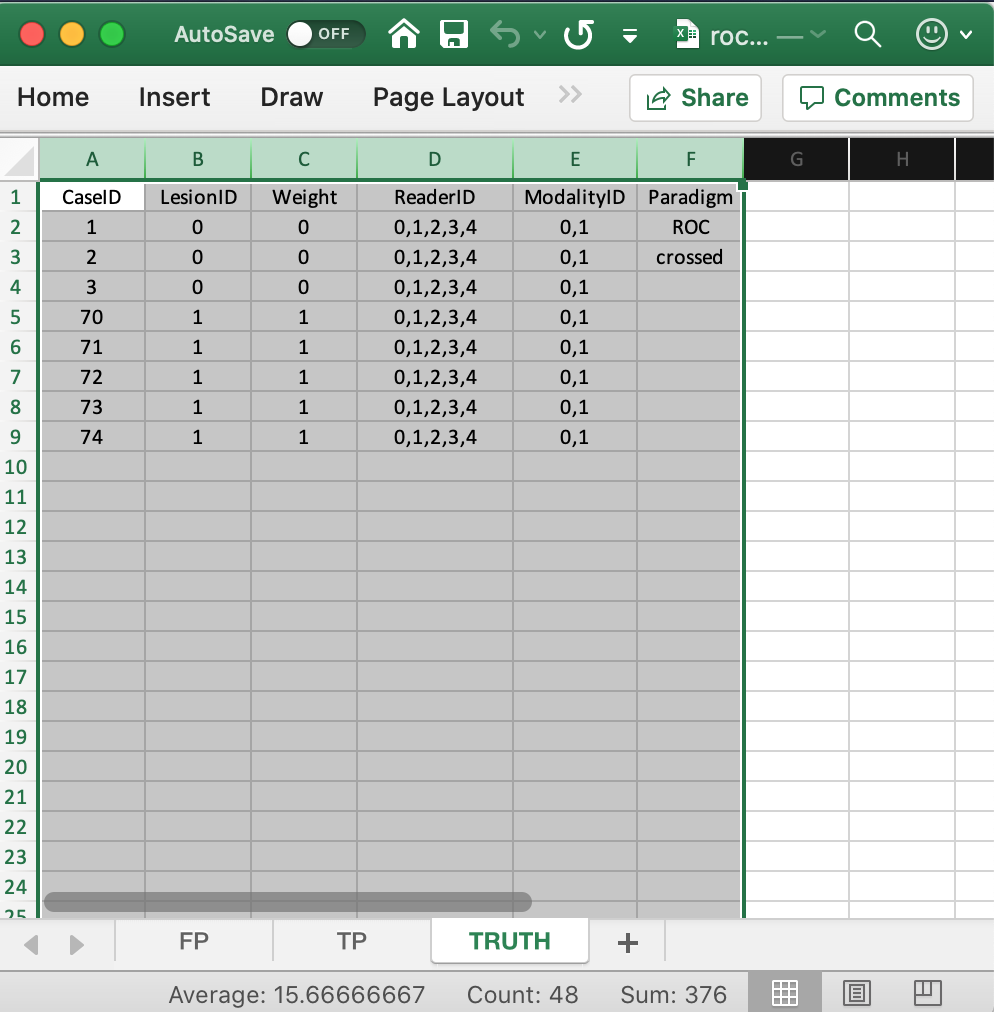
\includegraphics[width=0.5\linewidth,height=0.2\textheight]{images/rocCrTruth} 

}

\caption{Truth worksheet for file rocCr.xlsx}\label{fig:showRocCrTruthSheet}
\end{figure}

\hypertarget{the-structure-of-an-roc-dataset}{%
\section{The structure of an ROC dataset}\label{the-structure-of-an-roc-dataset}}

In the following code chunk the first statement retrieves the name of the data file, located in a hidden directory that one need not be concerned with. The second statement reads the file using the function \texttt{DfReadDataFile()} and saves it to object \texttt{x}. The third statement shows the structure of the dataset object \texttt{x}.

\begin{Shaded}
\begin{Highlighting}[]
\NormalTok{rocCr \textless{}{-}}\StringTok{ }\KeywordTok{system.file}\NormalTok{(}\StringTok{"extdata"}\NormalTok{, }\StringTok{"toyFiles/ROC/rocCr.xlsx"}\NormalTok{,}
                        \DataTypeTok{package =} \StringTok{"RJafroc"}\NormalTok{, }\DataTypeTok{mustWork =} \OtherTok{TRUE}\NormalTok{)}
\NormalTok{x \textless{}{-}}\StringTok{ }\KeywordTok{DfReadDataFile}\NormalTok{(rocCr, }\DataTypeTok{newExcelFileFormat =} \OtherTok{TRUE}\NormalTok{)}
\KeywordTok{str}\NormalTok{(x)}
\CommentTok{\#\textgreater{} List of 3}
\CommentTok{\#\textgreater{}  $ ratings     :List of 3}
\CommentTok{\#\textgreater{}   ..$ NL   : num [1:2, 1:5, 1:8, 1] 1 3 2 3 2 2 1 2 3 2 ...}
\CommentTok{\#\textgreater{}   ..$ LL   : num [1:2, 1:5, 1:5, 1] 5 5 5 5 5 5 5 5 5 5 ...}
\CommentTok{\#\textgreater{}   ..$ LL\_IL: logi NA}
\CommentTok{\#\textgreater{}  $ lesions     :List of 3}
\CommentTok{\#\textgreater{}   ..$ perCase: int [1:5] 1 1 1 1 1}
\CommentTok{\#\textgreater{}   ..$ IDs    : num [1:5, 1] 1 1 1 1 1}
\CommentTok{\#\textgreater{}   ..$ weights: num [1:5, 1] 1 1 1 1 1}
\CommentTok{\#\textgreater{}  $ descriptions:List of 7}
\CommentTok{\#\textgreater{}   ..$ fileName     : chr "rocCr"}
\CommentTok{\#\textgreater{}   ..$ type         : chr "ROC"}
\CommentTok{\#\textgreater{}   ..$ name         : logi NA}
\CommentTok{\#\textgreater{}   ..$ truthTableStr: num [1:2, 1:5, 1:8, 1:2] 1 1 1 1 1 1 1 1 1 1 ...}
\CommentTok{\#\textgreater{}   ..$ design       : chr "FCTRL"}
\CommentTok{\#\textgreater{}   ..$ modalityID   : Named chr [1:2] "0" "1"}
\CommentTok{\#\textgreater{}   .. ..{-} attr(*, "names")= chr [1:2] "0" "1"}
\CommentTok{\#\textgreater{}   ..$ readerID     : Named chr [1:5] "0" "1" "2" "3" ...}
\CommentTok{\#\textgreater{}   .. ..{-} attr(*, "names")= chr [1:5] "0" "1" "2" "3" ...}
\end{Highlighting}
\end{Shaded}

\begin{itemize}
\tightlist
\item
  In the above code chunk flag \texttt{newExcelFileFormat} is set to \texttt{TRUE} as otherwise columns D - F in the \texttt{Truth} worksheet are ignored and the dataset is assumed to be crossed, with \texttt{dataType} automatically determined from the contents of the FP and TP worksheets.
\item
  Flag \texttt{newExcelFileFormat\ =\ FALSE} is for compatibility with older JAFROC format Excel files, which did not have these columns in the \texttt{Truth} worksheet. Its usage is deprecated.
\item
  The dataset object \texttt{x} is a \texttt{list} variable with 3 members.
\item
  The \texttt{x\$NL} member, with dimension {[}2, 5, 8, 1{]}, contains the ratings of normal cases. The extra values in the third dimension, filled with \texttt{NAs}, are needed for compatibility with FROC datasets, as unlike ROC, false positives are possible on diseased cases.
\item
  The \texttt{x\$LL}, with dimension {[}2, 5, 5, 1{]}, contains the ratings of abnormal cases.
\item
  The \texttt{x\$lesionVector} member is a vector with 5 ones representing the 5 diseased cases in the dataset.
\item
  The \texttt{x\$lesionID} member is an array with 5 ones.
\item
  The \texttt{x\$lesionWeight} member is an array with 5 ones.
\item
  The \texttt{lesionVector}, \texttt{lesionID} and \texttt{lesionWeight} members are not used for ROC datasets. They are there for compatibility with FROC datasets.
\item
  The \texttt{dataType} member indicates that this is an \texttt{ROC} dataset.
\item
  The \texttt{x\$modalityID} member is a vector with two elements \texttt{"0"} and \texttt{"1"}, naming the two modalities.
\item
  The \texttt{x\$readerID} member is a vector with five elements \texttt{"0"}, \texttt{"1"}, \texttt{"2"}, \texttt{"3"} and \texttt{"4"}, naming the five readers.
\item
  The \texttt{x\$design} member is ; specifies the dataset design, which is ``CROSSED''.
\item
  The \texttt{x\$normalCases} member lists the integer names of the normal cases, .
\item
  The \texttt{x\$abnormalCases} member lists the integer names of the abnormal cases, .
\item
  The \texttt{x\$truthTableStr} member quantifies the structure of the dataset, as explained in prior chapters.
\end{itemize}

\hypertarget{rocExcelFPdataformat}{%
\section{The false positive (FP) ratings}\label{rocExcelFPdataformat}}

These are found in the \texttt{FP} or \texttt{NL} worksheet, see below.

\begin{figure}

{\centering 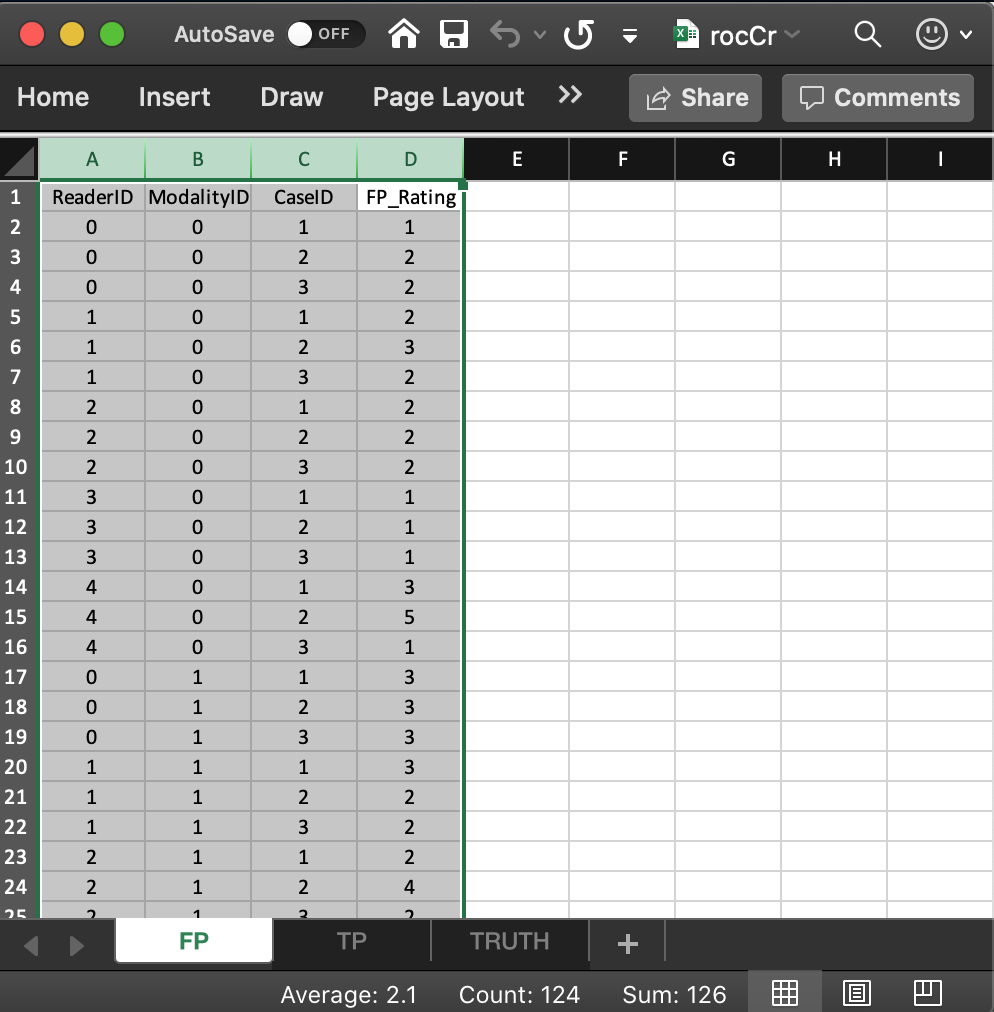
\includegraphics[width=0.5\linewidth,height=0.2\textheight]{images/rocCrFp} 

}

\caption{FP worksheet for file rocCr.xlsx}\label{fig:showRocCrFpSheet}
\end{figure}

\begin{itemize}
\tightlist
\item
  It consists of 4 columns, each of length 30 (= \# of modalities times number of readers times number of non-diseased cases).
\item
  \texttt{ReaderID}: the reader labels: \texttt{0}, \texttt{1}, \texttt{2}, \texttt{3} and \texttt{4}. Each reader label occurs 6 times (= \# of modalities times number of non-diseased cases).
\item
  \texttt{ModalityID}: the modality or treatment labels: \texttt{0} and \texttt{1}. Each label occurs 15 times (= \# of readers times number of non-diseased cases).
\item
  \texttt{CaseID}: the case labels for non-diseased cases: \texttt{1}, \texttt{2} and \texttt{3}. Each label occurs 10 times (= \# of modalities times \# of readers).
\item
  The label of a diseased case cannot occur in the FP worksheet. If it does the software generates an error.
\item
  \texttt{FP\_Rating}: the floating point ratings of non-diseased cases. Each row of this worksheet contains a rating corresponding to the values of \texttt{ReaderID}, \texttt{ModalityID} and \texttt{CaseID} for that row.
\end{itemize}

\hypertarget{rocExcelTPdataformat}{%
\section{The true positive (TP) ratings}\label{rocExcelTPdataformat}}

These are found in the \texttt{TP} or \texttt{LL} worksheet, see below.

\begin{figure}

{\centering 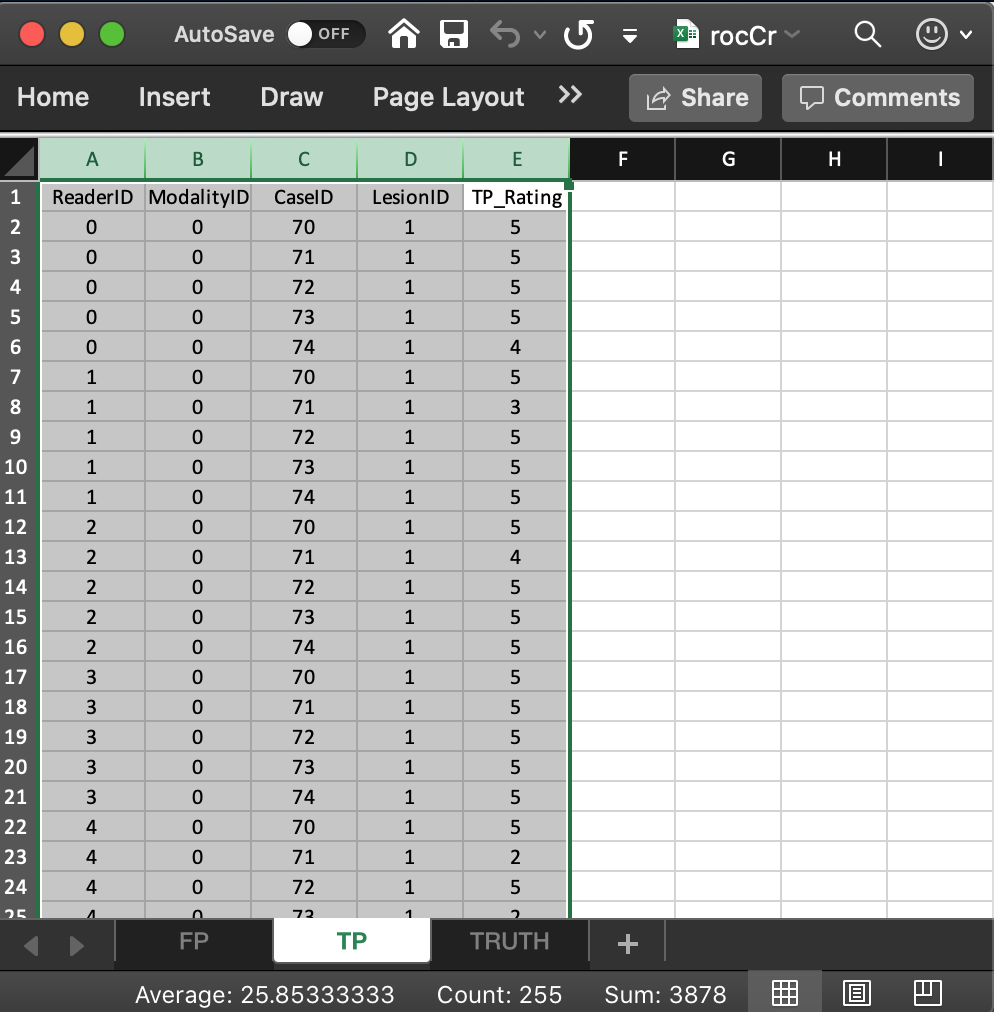
\includegraphics[width=0.5\linewidth,height=0.2\textheight]{images/rocCrTp} 

}

\caption{TP worksheet for file rocCr.xlsx}\label{fig:showRocCrTpSheet}
\end{figure}

\begin{itemize}
\tightlist
\item
  It consists of 5 columns, each of length 50 (= \# of modalities times number of readers times number of diseased cases).
\item
  \texttt{ReaderID}: the reader labels: \texttt{0}, \texttt{1}, \texttt{2}, \texttt{3} and \texttt{4}. Each reader label occurs 10 times (= \# of modalities times number of diseased cases).
\item
  \texttt{ModalityID}: the modality or treatment labels: \texttt{0} and \texttt{1}. Each label occurs 25 times (= \# of readers times number of diseased cases).
\item
  \texttt{LesionID}: For an ROC dataset this column contains fifty 1's (each diseased case has one lesion).
\item
  \texttt{CaseID}: the case labels for non-diseased cases: \texttt{70}, \texttt{71}, \texttt{72}, \texttt{73} and \texttt{74}. Each label occurs 10 times (= \# of modalities times \# of readers). The label of a non-diseased case cannot occur in the TP worksheet.
\item
  \texttt{TP\_Rating}: the floating point ratings of diseased cases. Each row of this worksheet contains a rating corresponding to the values of \texttt{ReaderID}, \texttt{ModalityID}, \texttt{LesionID} and \texttt{CaseID} for that row.
\end{itemize}

\hypertarget{correspondence-between-nl-member-of-dataset-and-the-fp-worksheet}{%
\section{\texorpdfstring{Correspondence between \texttt{NL} member of dataset and the \texttt{FP} worksheet}{Correspondence between NL member of dataset and the FP worksheet}}\label{correspondence-between-nl-member-of-dataset-and-the-fp-worksheet}}

\begin{itemize}
\tightlist
\item
  The list member \texttt{x\$NL} is an array with \texttt{dim\ =\ c(2,5,8,1)}.

  \begin{itemize}
  \tightlist
  \item
    The first dimension (2) comes from the number of modalities.
  \item
    The second dimension (5) comes from the number of readers.
  \item
    The third dimension (8) comes from the \textbf{total} number of cases.
  \item
    The fourth dimension is alway 1 for an ROC dataset.
  \end{itemize}
\item
  The value of \texttt{x\$NL{[}1,5,2,1{]}}, i.e., , corresponds to row 15 of the FP table, i.e., to \texttt{ModalityID} = 0, \texttt{ReaderID} = 4 and \texttt{CaseID} = 2.
\item
  The value of \texttt{x\$NL{[}2,3,2,1{]}}, i.e., , corresponds to row 24 of the FP table, i.e., to \texttt{ModalityID} 1, \texttt{ReaderID} 2 and \texttt{CaseID} 2.
\item
  All values for case index \textgreater{} 3 are \texttt{-Inf}. For example the value of \texttt{x\$NL{[}2,3,4,1{]}} is \texttt{-Inf}. This is because there are only 3 non-diseased cases. The extra length is needed for compatibility with FROC datasets.
\end{itemize}

\hypertarget{correspondence-between-ll-member-of-dataset-and-the-tp-worksheet}{%
\section{\texorpdfstring{Correspondence between \texttt{LL} member of dataset and the \texttt{TP} worksheet}{Correspondence between LL member of dataset and the TP worksheet}}\label{correspondence-between-ll-member-of-dataset-and-the-tp-worksheet}}

\begin{itemize}
\tightlist
\item
  The list member \texttt{x\$LL} is an array with \texttt{dim\ =\ c(2,5,5,1)}.

  \begin{itemize}
  \tightlist
  \item
    The first dimension (2) comes from the number of modalities.
  \item
    The second dimension (5) comes from the number of readers.
  \item
    The third dimension (5) comes from the number of diseased cases.
  \item
    The fourth dimension is alway 1 for an ROC dataset.
  \end{itemize}
\item
  The value of \texttt{x\$LL{[}1,1,5,1{]}}, i.e., , corresponds to row 6 of the TP table, i.e., to \texttt{ModalityID} = 0, \texttt{ReaderID} = 0 and \texttt{CaseID} = 74.
\item
  The value of \texttt{x\$LL{[}1,2,2,1{]}}, i.e., , corresponds to row 8 of the TP table, i.e., to \texttt{ModalityID} = 0, \texttt{ReaderID} = 1 and \texttt{CaseID} = 71.
\item
  There are no -Inf values in \texttt{x\$LL}: \texttt{any(x\$LL\ ==\ -Inf)} = FALSE.
\end{itemize}

\hypertarget{correspondence-using-the-which-function}{%
\section{\texorpdfstring{Correspondence using the \texttt{which} function}{Correspondence using the which function}}\label{correspondence-using-the-which-function}}

\begin{itemize}
\tightlist
\item
  Converting from \textbf{names} to \textbf{subscripts} (indicating position in an array) can be confusing.
\item
  The following example uses the \texttt{which} function to help out.
\item
  The first line says that the \texttt{abnormalCase} named 70 corresponds to subscript 1 in the LL array case dimension.
\item
  The second line prints the NL rating for \texttt{modalityID} = 0, \texttt{readerID} = 1 and \texttt{normalCases} = 1.
\item
  The third line prints the LL rating for \texttt{modalityID} = 0, \texttt{readerID} = 1 and \texttt{abnormalCases} = 70.
\item
  The last line shows what happens if one enters an invalid value for name; the result is a \texttt{numeric(0)}.
\item
  Note that in each of these examples, the last dimension is 1 because we are dealing with an ROC dataset.
\item
  The reader is encouraged to examine the correspondence between the NL and LL ratings and the Excel file using this method.
\end{itemize}

\begin{Shaded}
\begin{Highlighting}[]
\KeywordTok{which}\NormalTok{(x}\OperatorTok{$}\NormalTok{abnormalCases }\OperatorTok{==}\StringTok{ }\DecValTok{70}\NormalTok{)}
\CommentTok{\#\textgreater{} integer(0)}
\NormalTok{x}\OperatorTok{$}\NormalTok{NL[}\KeywordTok{which}\NormalTok{(x}\OperatorTok{$}\NormalTok{modalityID }\OperatorTok{==}\StringTok{ "0"}\NormalTok{),}\KeywordTok{which}\NormalTok{(x}\OperatorTok{$}\NormalTok{readerID }\OperatorTok{==}\StringTok{ "1"}\NormalTok{),}\KeywordTok{which}\NormalTok{(x}\OperatorTok{$}\NormalTok{normalCases }\OperatorTok{==}\StringTok{ }\DecValTok{1}\NormalTok{),}\DecValTok{1}\NormalTok{]}
\CommentTok{\#\textgreater{} NULL}
\NormalTok{x}\OperatorTok{$}\NormalTok{LL[}\KeywordTok{which}\NormalTok{(x}\OperatorTok{$}\NormalTok{modalityID }\OperatorTok{==}\StringTok{ "0"}\NormalTok{),}\KeywordTok{which}\NormalTok{(x}\OperatorTok{$}\NormalTok{readerID }\OperatorTok{==}\StringTok{ "1"}\NormalTok{),}\KeywordTok{which}\NormalTok{(x}\OperatorTok{$}\NormalTok{abnormalCases }\OperatorTok{==}\StringTok{ }\DecValTok{70}\NormalTok{),}\DecValTok{1}\NormalTok{]}
\CommentTok{\#\textgreater{} NULL}
\NormalTok{x}\OperatorTok{$}\NormalTok{LL[}\KeywordTok{which}\NormalTok{(x}\OperatorTok{$}\NormalTok{modalityID }\OperatorTok{==}\StringTok{ "a"}\NormalTok{),}\KeywordTok{which}\NormalTok{(x}\OperatorTok{$}\NormalTok{readerID }\OperatorTok{==}\StringTok{ "1"}\NormalTok{),}\KeywordTok{which}\NormalTok{(x}\OperatorTok{$}\NormalTok{abnormalCases }\OperatorTok{==}\StringTok{ }\DecValTok{70}\NormalTok{),}\DecValTok{1}\NormalTok{]}
\CommentTok{\#\textgreater{} NULL}
\end{Highlighting}
\end{Shaded}

\hypertarget{rocdataformat-Summary}{%
\section{Summary}\label{rocdataformat-Summary}}

\hypertarget{rocdataformat-Discussion}{%
\section{Discussion}\label{rocdataformat-Discussion}}

\hypertarget{rocdataformat-references}{%
\section{References}\label{rocdataformat-references}}

\hypertarget{frocdataformat}{%
\chapter{FROC data format}\label{frocdataformat}}

\hypertarget{purpose}{%
\section{Purpose}\label{purpose}}

\begin{itemize}
\tightlist
\item
  Explain the data format of the input Excel file for FROC datasets.
\item
  Explain the format of the FROC dataset.
\item
  Explain the lesion distribution array returned by \texttt{UtilLesionDistr()}.
\item
  Explain the lesion weights array returned by \texttt{UtilLesionWeightsDistr()}.
\item
  Details on the FROC paradigm are in my book.
\end{itemize}

\hypertarget{frocdataformatIntro}{%
\section{Introduction}\label{frocdataformatIntro}}

\begin{itemize}
\tightlist
\item
  See my book \citet{RN2680} for full details.
\item
  In the Free-response Receiver Operating Characteristic (FROC) paradigm \citep{RN761} the observer searches each case for signs of \textbf{localized disease} and marks and rates localized regions that are sufficiently suspicious for disease presence.
\item
  FROC data consists of \textbf{mark-rating pairs}, where each mark is a localized-region that was considered sufficiently suspicious for presence of a localized lesion and the rating is the corresponding confidence level.
\item
  By adopting a proximity criterion, each mark is classified by the investigator as a lesion localization (\texttt{LL}) - if it is close to a real lesion - or a non-lesion localization (\texttt{NL}) otherwise.
\item
  The observer assigns a rating to each region. The rating, as in the ROC paradigm, can be an integer or quasi-continuous (e.g., 0 -- 100), or a floating point value, as long as higher numbers represent greater confidence in presence of a lesion at the indicated region.
\end{itemize}

\hypertarget{frocExceldataformat}{%
\section{The Excel data format}\label{frocExceldataformat}}

The Excel file has three worsheets. These are named \texttt{Truth}, \texttt{NL} or \texttt{FP} and \texttt{LL} or \texttt{TP}.

\hypertarget{frocExcelTruthdataformat}{%
\section{\texorpdfstring{The \texttt{Truth} worksheet}{The Truth worksheet}}\label{frocExcelTruthdataformat}}

The \texttt{Truth} worksheet contains 6 columns: \texttt{CaseID}, \texttt{LesionID}, \texttt{Weight}, \texttt{ReaderID}, \texttt{ModalityID} and \texttt{Paradigm}.

\begin{itemize}
\tightlist
\item
  Since a diseased case may have more than one lesion, the first five columns contain \textbf{at least} as many rows as there are cases (images) in the dataset.
\item
  \texttt{CaseID}: unique \textbf{integers}, one per case, representing the cases in the dataset.
\item
  \texttt{LesionID}: integers 0, 1, 2, etc., with each 0 representing a non-diseased case, 1 representing the \emph{first} lesion on a diseased case, 2 representing the second lesion on a diseased case, if present, and so on.
\item
  The non-diseased cases are labeled \texttt{1}, \texttt{2} and \texttt{3}, while the diseased cases are labeled \texttt{70}, \texttt{71}, \texttt{72}, \texttt{73} and \texttt{74}.
\item
  There are 3 non-diseased cases in the dataset (the number of 0's in the \texttt{LesionID} column).
\item
  There are 5 diseased cases in the dataset (the number of 1's in the \texttt{LesionID} column of the \texttt{Truth} worksheet).
\item
  There are 3 readers in the dataset (each cell in the \texttt{ReaderID} column contains \texttt{0,\ 1,\ 2}).
\item
  There are 2 modalities in the dataset (each cell in the \texttt{ModalityID} column contains \texttt{0,\ 1}).
\item
  \texttt{Weight}: floating point; 0, for each non-diseased case, or values for each diseased case that add up to unity.\\
\item
  Diseased case \texttt{70} has two lesions, with \texttt{LesionID}s 1 and 2, and weights 0.3 and 0.7. Diseased case \texttt{71} has one lesion, with \texttt{LesionID} = 1, and \texttt{Weight} = 1. Diseased case \texttt{72} has three lesions, with \texttt{LesionID}s 1, 2 and 3 and weights 1/3 each. Diseased case \texttt{73} has two lesions, with \texttt{LesionID}s 1, and 2 and weights 0.1 and 0.9. Diseased case \texttt{74} has one lesion, with \texttt{LesionID} = 1 and \texttt{Weight} = 1.
\item
  \texttt{ReaderID}: a comma-separated listing of readers, each represented by a unique \textbf{integer}, that have interpreted the case. In the example shown below each cell has the value \texttt{0,\ 1,\ 2}. \textbf{Each cell has to be text formatted. Otherwise Excel will not accept it.}
\item
  \texttt{ModalityID}: a comma-separated listing of modalities (or treatments), each represented by a unique \textbf{integer}, that apply to each case. In the example each cell has the value \texttt{0,\ 1}. \textbf{Each cell has to be text formatted.}
\item
  \texttt{Paradigm}: In the example shown below, the contents are \texttt{FROC} and \texttt{crossed}. It informs the software that this is an \texttt{FROC} dataset and the design is ``crossed'', as in \textbf{TBA chapter xx}.
\end{itemize}

\begin{figure}

{\centering 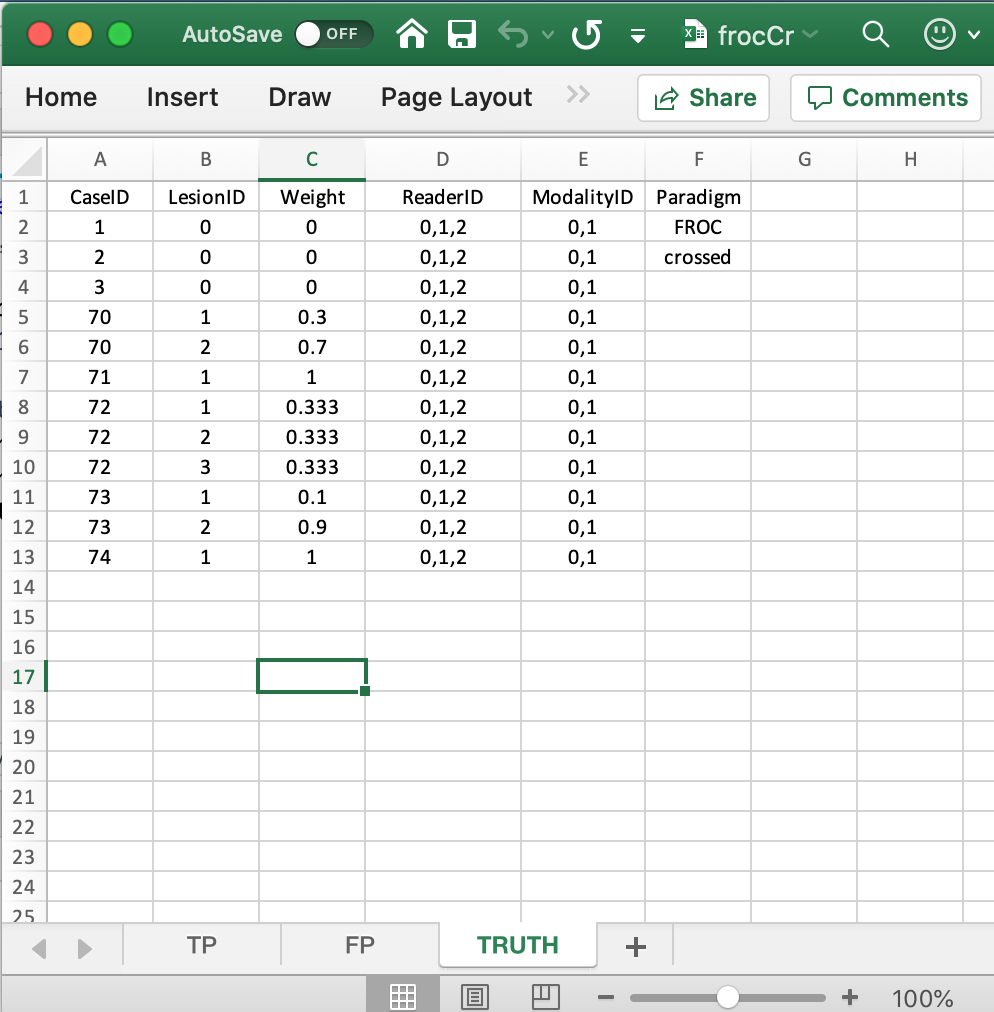
\includegraphics[width=0.5\linewidth,height=0.2\textheight]{images/frocCrTruth} 

}

\caption{Truth worksheet for file inst/extdata/toyFiles/FROC/frocCr.xlsx}\label{fig:frocCrTruth}
\end{figure}

\hypertarget{the-structure-of-an-froc-dataset}{%
\section{The structure of an FROC dataset}\label{the-structure-of-an-froc-dataset}}

The example shown above corresponds to Excel file \texttt{inst/extdata/toyFiles/FROC/frocCr.xlsx} in the project directory.

\begin{Shaded}
\begin{Highlighting}[]
\NormalTok{frocCr \textless{}{-}}\StringTok{ }\KeywordTok{system.file}\NormalTok{(}\StringTok{"extdata"}\NormalTok{, }\StringTok{"toyFiles/FROC/frocCr.xlsx"}\NormalTok{,}
                        \DataTypeTok{package =} \StringTok{"RJafroc"}\NormalTok{, }\DataTypeTok{mustWork =} \OtherTok{TRUE}\NormalTok{)}
\NormalTok{x \textless{}{-}}\StringTok{ }\KeywordTok{DfReadDataFile}\NormalTok{(frocCr, }\DataTypeTok{newExcelFileFormat =} \OtherTok{TRUE}\NormalTok{)}
\KeywordTok{str}\NormalTok{(x)}
\CommentTok{\#\textgreater{} List of 3}
\CommentTok{\#\textgreater{}  $ ratings     :List of 3}
\CommentTok{\#\textgreater{}   ..$ NL   : num [1:2, 1:3, 1:8, 1:2] 1.02 2.89 2.21 3.01 2.14 ...}
\CommentTok{\#\textgreater{}   ..$ LL   : num [1:2, 1:3, 1:5, 1:3] 5.28 5.2 5.14 4.77 4.66 4.87 3.01 3.27 3.31 3.19 ...}
\CommentTok{\#\textgreater{}   ..$ LL\_IL: logi NA}
\CommentTok{\#\textgreater{}  $ lesions     :List of 3}
\CommentTok{\#\textgreater{}   ..$ perCase: int [1:5] 2 1 3 2 1}
\CommentTok{\#\textgreater{}   ..$ IDs    : num [1:5, 1:3] 1 1 1 1 1 ...}
\CommentTok{\#\textgreater{}   ..$ weights: num [1:5, 1:3] 0.3 1 0.333 0.1 1 ...}
\CommentTok{\#\textgreater{}  $ descriptions:List of 7}
\CommentTok{\#\textgreater{}   ..$ fileName     : chr "frocCr"}
\CommentTok{\#\textgreater{}   ..$ type         : chr "FROC"}
\CommentTok{\#\textgreater{}   ..$ name         : logi NA}
\CommentTok{\#\textgreater{}   ..$ truthTableStr: num [1:2, 1:3, 1:8, 1:4] 1 1 1 1 1 1 1 1 1 1 ...}
\CommentTok{\#\textgreater{}   ..$ design       : chr "FCTRL"}
\CommentTok{\#\textgreater{}   ..$ modalityID   : Named chr [1:2] "0" "1"}
\CommentTok{\#\textgreater{}   .. ..{-} attr(*, "names")= chr [1:2] "0" "1"}
\CommentTok{\#\textgreater{}   ..$ readerID     : Named chr [1:3] "0" "1" "2"}
\CommentTok{\#\textgreater{}   .. ..{-} attr(*, "names")= chr [1:3] "0" "1" "2"}
\end{Highlighting}
\end{Shaded}

\begin{itemize}
\tightlist
\item
  This follows the general description in \textbf{TBA chapter xx}. The differences are described below.
\item
  The \texttt{x\$dataType} member indicates that this is an \texttt{FROC} dataset.
\item
  The \texttt{x\$lesionVector} member is a vector whose contents reflect the number of lesions in each diseased case, i.e., in the current example.
\item
  The \texttt{x\$lesionID} member indicates the labeling of the lesions in each diseased case.
\end{itemize}

\begin{Shaded}
\begin{Highlighting}[]
\NormalTok{x}\OperatorTok{$}\NormalTok{lesionID}
\CommentTok{\#\textgreater{} NULL}
\end{Highlighting}
\end{Shaded}

\begin{itemize}
\tightlist
\item
  This shows that the lesions on the first diseased case are labeled 1 and 2. The \texttt{-Inf} is a filler used to denote a missing value. The second diseased case has one lesion labeled 1. The third diseased case has three lesions labeled 1, 2 and 3, etc.
\item
  The \texttt{lesionWeight} member is the clinical importance of each lesion. Lacking specific clinical reasons, the lesions should be equally weighted; this is \emph{not} true for this toy dataset.
\end{itemize}

\begin{Shaded}
\begin{Highlighting}[]
\NormalTok{x}\OperatorTok{$}\NormalTok{lesionWeight}
\CommentTok{\#\textgreater{} NULL}
\end{Highlighting}
\end{Shaded}

\begin{itemize}
\tightlist
\item
  The first diseased case has two lesions, the first has weight 0.3 and the second has weight 0.7. The second diseased case has one lesion with weight 1.The third diseased case has three equally weighted lesions, each with weight 1/3. Etc.
\end{itemize}

\hypertarget{the-false-positive-fp-ratings}{%
\section{The false positive (FP) ratings}\label{the-false-positive-fp-ratings}}

These are found in the \texttt{FP} or \texttt{NL} worksheet, see below.

\begin{figure}

{\centering 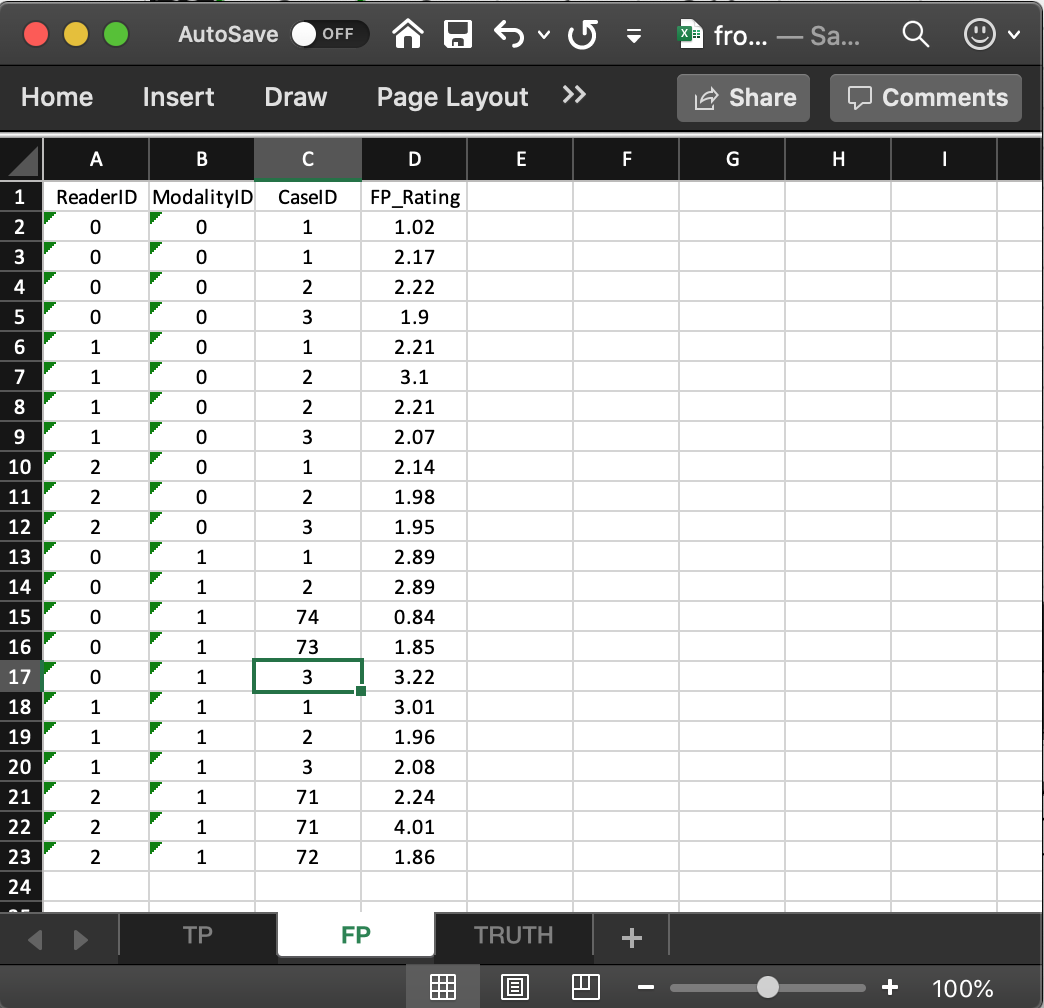
\includegraphics[width=0.5\linewidth,height=0.2\textheight]{images/frocCrNL} 

}

\caption{Fig. 2: FP/NL worksheet for file inst/extdata/toyFiles/FROC/frocCr.xlsx}\label{fig:frocCrNL}
\end{figure}

\begin{itemize}
\tightlist
\item
  It consists of 4 columns, of equal length. \textbf{The common length is unpredictable.} It could be zero if the dataset has no NL marks (a distinct possibility if the lesions are very easy to find and the modality and/or observer has high performance). All one knows is that the common length is an integer greater than or equal to zero.
\item
  In the example dataset, the common length is 0.
\item
  \texttt{ReaderID}: the reader labels: these must be \texttt{0}, \texttt{1}, or \texttt{2}, as declared in the \texttt{Truth} worksheet.
\item
  \texttt{ModalityID}: the modality labels: must be \texttt{0} or \texttt{1}, as declared in the \texttt{Truth} worksheet.
\item
  \texttt{CaseID}: the labels of cases with \texttt{NL} marks. In the FROC paradigm, \texttt{NL} events can occur on non-diseased \textbf{and} diseased cases.
\item
  \texttt{FP\_Rating}: the floating point ratings of \texttt{NL} marks. Each row of this worksheet yields a rating corresponding to the values of \texttt{ReaderID}, \texttt{ModalityID} and \texttt{CaseID} for that row.
\item
  For \texttt{ModalityID} 0, \texttt{ReaderID} 0 and \texttt{CaseID} 1 (the first non-diseased case declared in the \texttt{Truth} worksheet), there is a single \texttt{NL} mark that was rated , corresponding to row 2 of the \texttt{FP} worksheet.
\item
  Diseased cases with \texttt{NL} marks are also declared in the \texttt{FP} worksheet. Some examples are seen at rows 15, 16 and 21-23 of the \texttt{FP} worksheet.
\item
  Rows 21 and 22 show that \texttt{caseID} = 71 got two \texttt{NL} marks, rated .
\item
  That this is the \emph{only} case with two marks determines the length of the fourth dimension of the \texttt{x\$NL} list member, 0 in the current example. Absent this case, the length would have been one.
\item
  In general, the case with the most \texttt{NL} marks determines the length of the fourth dimension of the \texttt{x\$NL} list member.
\item
  The reader should convince oneself that the ratings in \texttt{x\$NL} reflect the contents of the \texttt{FP} worksheet.
\end{itemize}

\hypertarget{the-true-positive-tp-ratings}{%
\section{The true positive (TP) ratings}\label{the-true-positive-tp-ratings}}

These are found in the \texttt{TP} or \texttt{LL} worksheet, see below.

\begin{figure}

{\centering 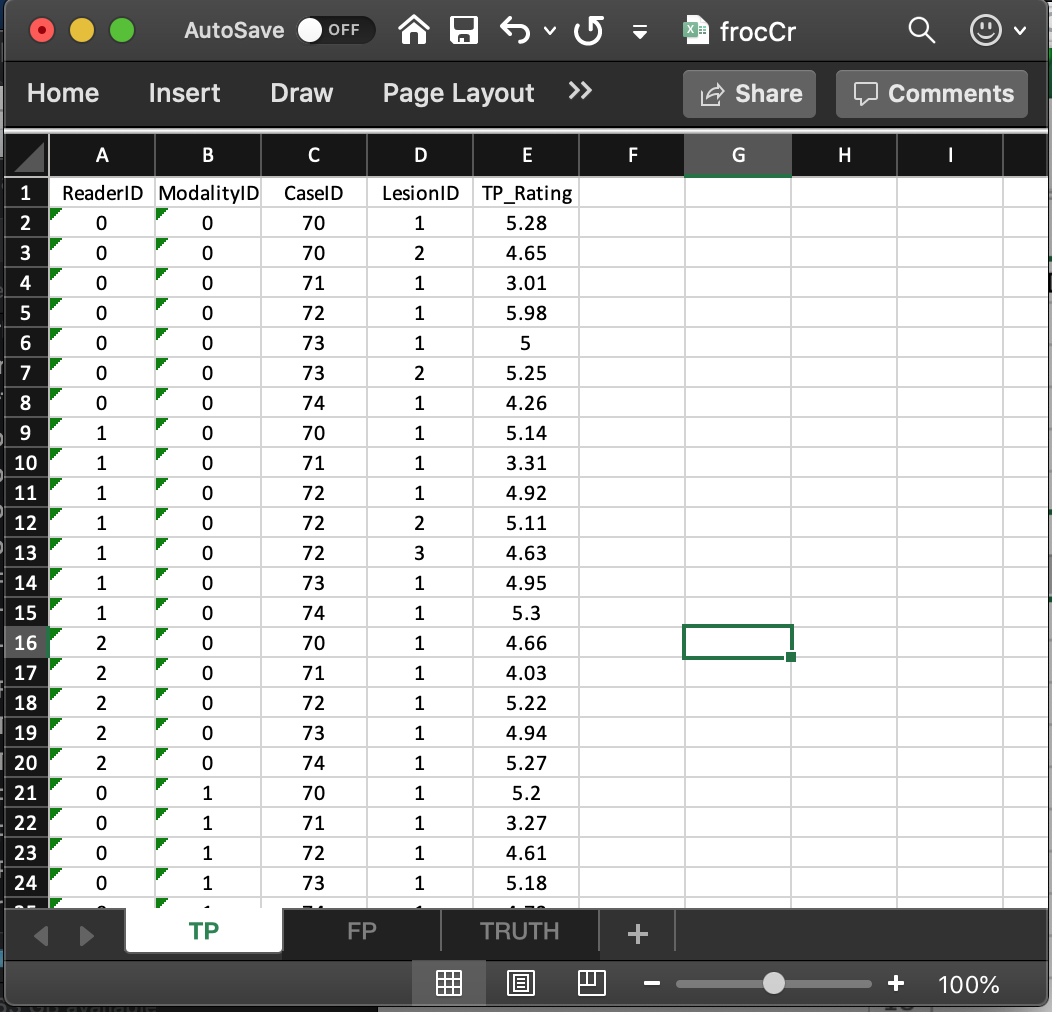
\includegraphics[width=0.5\linewidth,height=0.2\textheight]{images/frocCrLL} 

}

\caption{Fig. 3: TP/LL worksheet for file inst/extdata/toyFiles/FROC/frocCr.xlsx}\label{fig:frocCrLL}
\end{figure}

\begin{itemize}
\tightlist
\item
  This worksheet can only have diseased cases. The presence of a non-diseased case in this worksheet will generate an error.
\item
  The common vertical length, 31 in this example, is a-priori unpredictable. Given the structure of the \texttt{Truth} worsheet for this dataset, the maximum length would be 9 times 2 times 3, assuming every lesion is marked for each modality, reader and diseased case. The 9 comes from the total number of non-zero entries in the \texttt{LesionID} column of the \texttt{Truth} worksheet.
\item
  The fact that the length is smaller than the maximum length means that there are combinations of modality, reader and diseased cases on which some lesions were not marked.
\item
  As an example, the first lesion in \texttt{CaseID} equal to \texttt{70} was marked (and rated ) in \texttt{ModalityID} \texttt{0} and \texttt{ReaderID} \texttt{0}.
\item
  The length of the fourth dimension of the \texttt{x\$LL} list member, 0 in the present example, is determined by the diseased case with the most lesions in the \texttt{Truth} worksheet.
\item
  The reader should convince oneself that the ratings in \texttt{x\$LL} reflect the contents of the \texttt{TP} worksheet.
\end{itemize}

\hypertarget{on-the-distribution-of-numbers-of-lesions-in-abnormal-cases}{%
\section{On the distribution of numbers of lesions in abnormal cases}\label{on-the-distribution-of-numbers-of-lesions-in-abnormal-cases}}

\begin{itemize}
\tightlist
\item
  Consider a much larger dataset, \texttt{dataset11}, with structure as shown below:
\end{itemize}

\begin{Shaded}
\begin{Highlighting}[]
\NormalTok{x \textless{}{-}}\StringTok{ }\NormalTok{dataset11}
\KeywordTok{str}\NormalTok{(x)}
\CommentTok{\#\textgreater{} List of 3}
\CommentTok{\#\textgreater{}  $ ratings     :List of 3}
\CommentTok{\#\textgreater{}   ..$ NL   : num [1:4, 1:5, 1:158, 1:4] {-}Inf {-}Inf {-}Inf {-}Inf {-}Inf ...}
\CommentTok{\#\textgreater{}   ..$ LL   : num [1:4, 1:5, 1:115, 1:20] {-}Inf {-}Inf {-}Inf {-}Inf {-}Inf ...}
\CommentTok{\#\textgreater{}   ..$ LL\_IL: logi NA}
\CommentTok{\#\textgreater{}  $ lesions     :List of 3}
\CommentTok{\#\textgreater{}   ..$ perCase: int [1:115] 6 4 7 1 3 3 3 8 11 2 ...}
\CommentTok{\#\textgreater{}   ..$ IDs    : num [1:115, 1:20] 1 1 1 1 1 1 1 1 1 1 ...}
\CommentTok{\#\textgreater{}   ..$ weights: num [1:115, 1:20] 0.167 0.25 0.143 1 0.333 ...}
\CommentTok{\#\textgreater{}  $ descriptions:List of 7}
\CommentTok{\#\textgreater{}   ..$ fileName     : chr "dataset11"}
\CommentTok{\#\textgreater{}   ..$ type         : chr "FROC"}
\CommentTok{\#\textgreater{}   ..$ name         : chr "DOBBINS{-}1"}
\CommentTok{\#\textgreater{}   ..$ truthTableStr: num [1:4, 1:5, 1:158, 1:21] 1 1 1 1 1 1 1 1 1 1 ...}
\CommentTok{\#\textgreater{}   ..$ design       : chr "FCTRL"}
\CommentTok{\#\textgreater{}   ..$ modalityID   : Named chr [1:4] "1" "2" "3" "4"}
\CommentTok{\#\textgreater{}   .. ..{-} attr(*, "names")= chr [1:4] "1" "2" "3" "4"}
\CommentTok{\#\textgreater{}   ..$ readerID     : Named chr [1:5] "1" "2" "3" "4" ...}
\CommentTok{\#\textgreater{}   .. ..{-} attr(*, "names")= chr [1:5] "1" "2" "3" "4" ...}
\end{Highlighting}
\end{Shaded}

\begin{itemize}
\tightlist
\item
  Focus for now in the 115 abnormal cases.
\item
  The numbers of lesions in these cases is contained in \texttt{x\$lesionVector}.
\end{itemize}

\begin{Shaded}
\begin{Highlighting}[]
\NormalTok{x}\OperatorTok{$}\NormalTok{lesions}\OperatorTok{$}\NormalTok{perCase}
\CommentTok{\#\textgreater{}   [1]  6  4  7  1  3  3  3  8 11  2  4  6  2 16  5  2  8  3  4  7 11  1  4  3  4}
\CommentTok{\#\textgreater{}  [26]  4  7  3  2  5  2  2  7  6  6  4 10 20 12  6  4  7 12  5  1  1  5  1  2  8}
\CommentTok{\#\textgreater{}  [51]  3  1  2  2  3  2  8 16 10  1  2  2  6  3  2  2  4  6 10 11  1  2  6  2  4}
\CommentTok{\#\textgreater{}  [76]  5  2  9  6  6  8  3  8  7  1  1  6  3  2  1  9  8  8  2  2 12  1  1  1  1}
\CommentTok{\#\textgreater{} [101]  1  3  1  2  2  1  1  1  1  3  1  1  1  2  1}
\end{Highlighting}
\end{Shaded}

\begin{itemize}
\tightlist
\item
  For example, the first abnormal case contains 6 lesions, the second contains 4 lesions, the third contains 7 lesions, etc. and the last abnormal case contains 1 lesion.
\item
  To get an idea of the distribution of the numbers of lesions per abnormal cases, one could interrogate this vector as shown below using the \texttt{which()} function:
\end{itemize}

\begin{Shaded}
\begin{Highlighting}[]
\ControlFlowTok{for}\NormalTok{ (el }\ControlFlowTok{in} \DecValTok{1}\OperatorTok{:}\KeywordTok{max}\NormalTok{(x}\OperatorTok{$}\NormalTok{lesions}\OperatorTok{$}\NormalTok{perCase)) }\KeywordTok{cat}\NormalTok{(}
  \StringTok{"abnormal cases with"}\NormalTok{, el, }\StringTok{"lesions = "}\NormalTok{, }
  \KeywordTok{length}\NormalTok{(}\KeywordTok{which}\NormalTok{(x}\OperatorTok{$}\NormalTok{lesionVector }\OperatorTok{==}\StringTok{ }\NormalTok{el)), }\StringTok{"}\CharTok{\textbackslash{}n}\StringTok{"}\NormalTok{)}
\CommentTok{\#\textgreater{} abnormal cases with 1 lesions =  0 }
\CommentTok{\#\textgreater{} abnormal cases with 2 lesions =  0 }
\CommentTok{\#\textgreater{} abnormal cases with 3 lesions =  0 }
\CommentTok{\#\textgreater{} abnormal cases with 4 lesions =  0 }
\CommentTok{\#\textgreater{} abnormal cases with 5 lesions =  0 }
\CommentTok{\#\textgreater{} abnormal cases with 6 lesions =  0 }
\CommentTok{\#\textgreater{} abnormal cases with 7 lesions =  0 }
\CommentTok{\#\textgreater{} abnormal cases with 8 lesions =  0 }
\CommentTok{\#\textgreater{} abnormal cases with 9 lesions =  0 }
\CommentTok{\#\textgreater{} abnormal cases with 10 lesions =  0 }
\CommentTok{\#\textgreater{} abnormal cases with 11 lesions =  0 }
\CommentTok{\#\textgreater{} abnormal cases with 12 lesions =  0 }
\CommentTok{\#\textgreater{} abnormal cases with 13 lesions =  0 }
\CommentTok{\#\textgreater{} abnormal cases with 14 lesions =  0 }
\CommentTok{\#\textgreater{} abnormal cases with 15 lesions =  0 }
\CommentTok{\#\textgreater{} abnormal cases with 16 lesions =  0 }
\CommentTok{\#\textgreater{} abnormal cases with 17 lesions =  0 }
\CommentTok{\#\textgreater{} abnormal cases with 18 lesions =  0 }
\CommentTok{\#\textgreater{} abnormal cases with 19 lesions =  0 }
\CommentTok{\#\textgreater{} abnormal cases with 20 lesions =  0}
\end{Highlighting}
\end{Shaded}

\begin{itemize}
\tightlist
\item
  This tells us that 25 cases contain 1 lesion
\item
  Likewise, 23 cases contain 2 lesions
\item
  Etc.
\end{itemize}

\hypertarget{definition-of-lesdistr-array}{%
\subsection{\texorpdfstring{Definition of \texttt{lesDistr} array}{Definition of lesDistr array}}\label{definition-of-lesdistr-array}}

\begin{itemize}
\tightlist
\item
  Let us ask what is the fraction of (abnormal) cases with 1 lesion, 2 lesions etc.
\end{itemize}

\begin{Shaded}
\begin{Highlighting}[]
\ControlFlowTok{for}\NormalTok{ (el }\ControlFlowTok{in} \DecValTok{1}\OperatorTok{:}\KeywordTok{max}\NormalTok{(x}\OperatorTok{$}\NormalTok{lesions}\OperatorTok{$}\NormalTok{perCase)) }\KeywordTok{cat}\NormalTok{(}\StringTok{"fraction of abnormal cases with"}\NormalTok{, el, }\StringTok{"lesions = "}\NormalTok{, }
                                              \KeywordTok{length}\NormalTok{(}\KeywordTok{which}\NormalTok{(x}\OperatorTok{$}\NormalTok{lesions}\OperatorTok{$}\NormalTok{perCase }\OperatorTok{==}\StringTok{ }\NormalTok{el))}\OperatorTok{/}\KeywordTok{length}\NormalTok{(x}\OperatorTok{$}\NormalTok{ratings}\OperatorTok{$}\NormalTok{LL[}\DecValTok{1}\NormalTok{,}\DecValTok{1}\NormalTok{,,}\DecValTok{1}\NormalTok{]), }\StringTok{"}\CharTok{\textbackslash{}n}\StringTok{"}\NormalTok{)}
\CommentTok{\#\textgreater{} fraction of abnormal cases with 1 lesions =  0.2173913 }
\CommentTok{\#\textgreater{} fraction of abnormal cases with 2 lesions =  0.2 }
\CommentTok{\#\textgreater{} fraction of abnormal cases with 3 lesions =  0.1130435 }
\CommentTok{\#\textgreater{} fraction of abnormal cases with 4 lesions =  0.08695652 }
\CommentTok{\#\textgreater{} fraction of abnormal cases with 5 lesions =  0.04347826 }
\CommentTok{\#\textgreater{} fraction of abnormal cases with 6 lesions =  0.09565217 }
\CommentTok{\#\textgreater{} fraction of abnormal cases with 7 lesions =  0.05217391 }
\CommentTok{\#\textgreater{} fraction of abnormal cases with 8 lesions =  0.06956522 }
\CommentTok{\#\textgreater{} fraction of abnormal cases with 9 lesions =  0.0173913 }
\CommentTok{\#\textgreater{} fraction of abnormal cases with 10 lesions =  0.02608696 }
\CommentTok{\#\textgreater{} fraction of abnormal cases with 11 lesions =  0.02608696 }
\CommentTok{\#\textgreater{} fraction of abnormal cases with 12 lesions =  0.02608696 }
\CommentTok{\#\textgreater{} fraction of abnormal cases with 13 lesions =  0 }
\CommentTok{\#\textgreater{} fraction of abnormal cases with 14 lesions =  0 }
\CommentTok{\#\textgreater{} fraction of abnormal cases with 15 lesions =  0 }
\CommentTok{\#\textgreater{} fraction of abnormal cases with 16 lesions =  0.0173913 }
\CommentTok{\#\textgreater{} fraction of abnormal cases with 17 lesions =  0 }
\CommentTok{\#\textgreater{} fraction of abnormal cases with 18 lesions =  0 }
\CommentTok{\#\textgreater{} fraction of abnormal cases with 19 lesions =  0 }
\CommentTok{\#\textgreater{} fraction of abnormal cases with 20 lesions =  0.008695652}
\end{Highlighting}
\end{Shaded}

\begin{itemize}
\tightlist
\item
  This tells us that fraction 0.217 of (abnormal) cases contain 1 lesion
\item
  And fraction 0.2 of (abnormal) cases contain 2 lesions
\item
  Etc.
\item
  This information is contained the the \texttt{lesDistr} array
\item
  It is coded in the \texttt{Utility} function \texttt{UtilLesionDistr()}
\end{itemize}

\begin{Shaded}
\begin{Highlighting}[]
\NormalTok{lesDistr \textless{}{-}}\StringTok{ }\KeywordTok{UtilLesionDistr}\NormalTok{(x)}
\NormalTok{lesDistr}
\CommentTok{\#\textgreater{}       [,1]        [,2]}
\CommentTok{\#\textgreater{}  [1,]    1 0.217391304}
\CommentTok{\#\textgreater{}  [2,]    2 0.200000000}
\CommentTok{\#\textgreater{}  [3,]    3 0.113043478}
\CommentTok{\#\textgreater{}  [4,]    4 0.086956522}
\CommentTok{\#\textgreater{}  [5,]    5 0.043478261}
\CommentTok{\#\textgreater{}  [6,]    6 0.095652174}
\CommentTok{\#\textgreater{}  [7,]    7 0.052173913}
\CommentTok{\#\textgreater{}  [8,]    8 0.069565217}
\CommentTok{\#\textgreater{}  [9,]    9 0.017391304}
\CommentTok{\#\textgreater{} [10,]   10 0.026086957}
\CommentTok{\#\textgreater{} [11,]   11 0.026086957}
\CommentTok{\#\textgreater{} [12,]   12 0.026086957}
\CommentTok{\#\textgreater{} [13,]   16 0.017391304}
\CommentTok{\#\textgreater{} [14,]   20 0.008695652}
\end{Highlighting}
\end{Shaded}

\begin{itemize}
\tightlist
\item
  The \texttt{UtilLesionDistr()} function returns an array with two columns and number of rows equal to the number of distinct values of lesions per case.
\item
  The first column contains the number of distinct values of lesions per case, 14 in the current example.
\item
  The second column contains the fraction of diseased cases with the number of lesions indicated in the first column.
\item
  The second column must sum to unity
\end{itemize}

\begin{Shaded}
\begin{Highlighting}[]
\KeywordTok{sum}\NormalTok{(}\KeywordTok{UtilLesionDistr}\NormalTok{(x)[,}\DecValTok{2}\NormalTok{])}
\CommentTok{\#\textgreater{} [1] 1}
\end{Highlighting}
\end{Shaded}

\begin{itemize}
\tightlist
\item
  The lesion distribution array will come in handy when it comes to predicting the operating characteristics from using the Radiological Search Model (RSM), as detailed in Chapter 17 of my book.
\end{itemize}

\hypertarget{definition-of-leswghtdistr-array}{%
\section{\texorpdfstring{Definition of \texttt{lesWghtDistr} array}{Definition of lesWghtDistr array}}\label{definition-of-leswghtdistr-array}}

\begin{itemize}
\tightlist
\item
  This is returned by \texttt{UtilLesionWeightsDistr()}.
\item
  This contains the same number of rows as \texttt{lesDistr}.
\item
  The number of columns is one plus the number of rows as \texttt{lesDistr}.
\item
  The first column contains the number of distinct values of lesions per case, 14 in the current example.
\item
  The second column contains the weights of cases with number of lesions per case corresponding to row 1.
\item
  The third column contains the weights of cases with number of lesions per case corresponding to row 2.
\item
  Etc.
\item
  Missing values are filled with \texttt{-Inf}.
\end{itemize}

\begin{Shaded}
\begin{Highlighting}[]
\NormalTok{lesWghtDistr \textless{}{-}}\StringTok{ }\KeywordTok{UtilLesionWeightsDistr}\NormalTok{(x)}
\KeywordTok{cat}\NormalTok{(}\StringTok{"dim(lesDistr) ="}\NormalTok{, }\KeywordTok{dim}\NormalTok{(lesDistr),}\StringTok{"}\CharTok{\textbackslash{}n}\StringTok{"}\NormalTok{)}
\CommentTok{\#\textgreater{} dim(lesDistr) = 14 2}
\KeywordTok{cat}\NormalTok{(}\StringTok{"dim(lesWghtDistr) ="}\NormalTok{, }\KeywordTok{dim}\NormalTok{(lesWghtDistr),}\StringTok{"}\CharTok{\textbackslash{}n}\StringTok{"}\NormalTok{)}
\CommentTok{\#\textgreater{} dim(lesWghtDistr) = 14 21}
\KeywordTok{cat}\NormalTok{(}\StringTok{"lesWghtDistr = }\CharTok{\textbackslash{}n\textbackslash{}n}\StringTok{"}\NormalTok{)}
\CommentTok{\#\textgreater{} lesWghtDistr =}
\NormalTok{lesWghtDistr}
\CommentTok{\#\textgreater{}       [,1]       [,2]       [,3]       [,4]       [,5]       [,6]       [,7]}
\CommentTok{\#\textgreater{}  [1,]    1 1.00000000       {-}Inf       {-}Inf       {-}Inf       {-}Inf       {-}Inf}
\CommentTok{\#\textgreater{}  [2,]    2 0.50000000 0.50000000       {-}Inf       {-}Inf       {-}Inf       {-}Inf}
\CommentTok{\#\textgreater{}  [3,]    3 0.33333333 0.33333333 0.33333333       {-}Inf       {-}Inf       {-}Inf}
\CommentTok{\#\textgreater{}  [4,]    4 0.25000000 0.25000000 0.25000000 0.25000000       {-}Inf       {-}Inf}
\CommentTok{\#\textgreater{}  [5,]    5 0.20000000 0.20000000 0.20000000 0.20000000 0.20000000       {-}Inf}
\CommentTok{\#\textgreater{}  [6,]    6 0.16666667 0.16666667 0.16666667 0.16666667 0.16666667 0.16666667}
\CommentTok{\#\textgreater{}  [7,]    7 0.14285714 0.14285714 0.14285714 0.14285714 0.14285714 0.14285714}
\CommentTok{\#\textgreater{}  [8,]    8 0.12500000 0.12500000 0.12500000 0.12500000 0.12500000 0.12500000}
\CommentTok{\#\textgreater{}  [9,]    9 0.11111111 0.11111111 0.11111111 0.11111111 0.11111111 0.11111111}
\CommentTok{\#\textgreater{} [10,]   10 0.10000000 0.10000000 0.10000000 0.10000000 0.10000000 0.10000000}
\CommentTok{\#\textgreater{} [11,]   11 0.09090909 0.09090909 0.09090909 0.09090909 0.09090909 0.09090909}
\CommentTok{\#\textgreater{} [12,]   12 0.08333333 0.08333333 0.08333333 0.08333333 0.08333333 0.08333333}
\CommentTok{\#\textgreater{} [13,]   16 0.06250000 0.06250000 0.06250000 0.06250000 0.06250000 0.06250000}
\CommentTok{\#\textgreater{} [14,]   20 0.05000000 0.05000000 0.05000000 0.05000000 0.05000000 0.05000000}
\CommentTok{\#\textgreater{}             [,8]       [,9]      [,10]      [,11]      [,12]      [,13]  [,14]}
\CommentTok{\#\textgreater{}  [1,]       {-}Inf       {-}Inf       {-}Inf       {-}Inf       {-}Inf       {-}Inf   {-}Inf}
\CommentTok{\#\textgreater{}  [2,]       {-}Inf       {-}Inf       {-}Inf       {-}Inf       {-}Inf       {-}Inf   {-}Inf}
\CommentTok{\#\textgreater{}  [3,]       {-}Inf       {-}Inf       {-}Inf       {-}Inf       {-}Inf       {-}Inf   {-}Inf}
\CommentTok{\#\textgreater{}  [4,]       {-}Inf       {-}Inf       {-}Inf       {-}Inf       {-}Inf       {-}Inf   {-}Inf}
\CommentTok{\#\textgreater{}  [5,]       {-}Inf       {-}Inf       {-}Inf       {-}Inf       {-}Inf       {-}Inf   {-}Inf}
\CommentTok{\#\textgreater{}  [6,]       {-}Inf       {-}Inf       {-}Inf       {-}Inf       {-}Inf       {-}Inf   {-}Inf}
\CommentTok{\#\textgreater{}  [7,] 0.14285714       {-}Inf       {-}Inf       {-}Inf       {-}Inf       {-}Inf   {-}Inf}
\CommentTok{\#\textgreater{}  [8,] 0.12500000 0.12500000       {-}Inf       {-}Inf       {-}Inf       {-}Inf   {-}Inf}
\CommentTok{\#\textgreater{}  [9,] 0.11111111 0.11111111 0.11111111       {-}Inf       {-}Inf       {-}Inf   {-}Inf}
\CommentTok{\#\textgreater{} [10,] 0.10000000 0.10000000 0.10000000 0.10000000       {-}Inf       {-}Inf   {-}Inf}
\CommentTok{\#\textgreater{} [11,] 0.09090909 0.09090909 0.09090909 0.09090909 0.09090909       {-}Inf   {-}Inf}
\CommentTok{\#\textgreater{} [12,] 0.08333333 0.08333333 0.08333333 0.08333333 0.08333333 0.08333333   {-}Inf}
\CommentTok{\#\textgreater{} [13,] 0.06250000 0.06250000 0.06250000 0.06250000 0.06250000 0.06250000 0.0625}
\CommentTok{\#\textgreater{} [14,] 0.05000000 0.05000000 0.05000000 0.05000000 0.05000000 0.05000000 0.0500}
\CommentTok{\#\textgreater{}        [,15]  [,16]  [,17] [,18] [,19] [,20] [,21]}
\CommentTok{\#\textgreater{}  [1,]   {-}Inf   {-}Inf   {-}Inf  {-}Inf  {-}Inf  {-}Inf  {-}Inf}
\CommentTok{\#\textgreater{}  [2,]   {-}Inf   {-}Inf   {-}Inf  {-}Inf  {-}Inf  {-}Inf  {-}Inf}
\CommentTok{\#\textgreater{}  [3,]   {-}Inf   {-}Inf   {-}Inf  {-}Inf  {-}Inf  {-}Inf  {-}Inf}
\CommentTok{\#\textgreater{}  [4,]   {-}Inf   {-}Inf   {-}Inf  {-}Inf  {-}Inf  {-}Inf  {-}Inf}
\CommentTok{\#\textgreater{}  [5,]   {-}Inf   {-}Inf   {-}Inf  {-}Inf  {-}Inf  {-}Inf  {-}Inf}
\CommentTok{\#\textgreater{}  [6,]   {-}Inf   {-}Inf   {-}Inf  {-}Inf  {-}Inf  {-}Inf  {-}Inf}
\CommentTok{\#\textgreater{}  [7,]   {-}Inf   {-}Inf   {-}Inf  {-}Inf  {-}Inf  {-}Inf  {-}Inf}
\CommentTok{\#\textgreater{}  [8,]   {-}Inf   {-}Inf   {-}Inf  {-}Inf  {-}Inf  {-}Inf  {-}Inf}
\CommentTok{\#\textgreater{}  [9,]   {-}Inf   {-}Inf   {-}Inf  {-}Inf  {-}Inf  {-}Inf  {-}Inf}
\CommentTok{\#\textgreater{} [10,]   {-}Inf   {-}Inf   {-}Inf  {-}Inf  {-}Inf  {-}Inf  {-}Inf}
\CommentTok{\#\textgreater{} [11,]   {-}Inf   {-}Inf   {-}Inf  {-}Inf  {-}Inf  {-}Inf  {-}Inf}
\CommentTok{\#\textgreater{} [12,]   {-}Inf   {-}Inf   {-}Inf  {-}Inf  {-}Inf  {-}Inf  {-}Inf}
\CommentTok{\#\textgreater{} [13,] 0.0625 0.0625 0.0625  {-}Inf  {-}Inf  {-}Inf  {-}Inf}
\CommentTok{\#\textgreater{} [14,] 0.0500 0.0500 0.0500  0.05  0.05  0.05  0.05}
\end{Highlighting}
\end{Shaded}

\begin{itemize}
\tightlist
\item
  Row 3 corresponds to 3 lesions per case and the weights are 1/3, 1/3 and 1/3.
\item
  Row 13 corresponds to 16 lesions per case and the weights are 0.06250000, 0.06250000, \ldots, repeated 13 times.
\item
  Note that the number of rows is less than the maximum number of lesions per case (20).
\item
  This is because some configurations of lesions per case (e.g., cases with 13 lesions per case) do not occur in this dataset.
\end{itemize}

\hypertarget{frocdataformat-Summary}{%
\section{Summary}\label{frocdataformat-Summary}}

\begin{itemize}
\tightlist
\item
  The FROC dataset has far less regularity in structure as compared to an ROC dataset.
\item
  The length of the first dimension of either \texttt{x\$NL} or \texttt{x\$LL} list members is the total number of modalities, 2 in the current example.
\item
  The length of the second dimension of either \texttt{x\$NL} or \texttt{x\$LL} list members is the total number of readers, 3 in the current example.
\item
  The length of the third dimension of \texttt{x\$NL} is the total number of cases, 8 in the current example. The first three positions account for \texttt{NL} marks on non-diseased cases and the remaining 5 positions account for \texttt{NL} marks on diseased cases.
\item
  The length of the third dimension of \texttt{x\$LL} is the total number of diseased cases, 5 in the current example.
\item
  The length of the fourth dimension of \texttt{x\$NL} is determined by the case (diseased or non-diseased) with the most \texttt{NL} marks, 2 in the current example.
\item
  The length of the fourth dimension of \texttt{x\$LL} is determined by the diseased case with the most lesions, 3 in the current example.
\end{itemize}

\hypertarget{frocdataformat-Discussion}{%
\section{Discussion}\label{frocdataformat-Discussion}}

\hypertarget{frocdataformat-references}{%
\section{References}\label{frocdataformat-references}}

  \bibliography{packages.bib,myRefs.bib}

\end{document}
